% !TeX spellcheck = en_GB
\documentclass[12pt,a4paper,openright,twoside]{book}
\usepackage[utf8]{inputenc}
\usepackage{phd-thesis}
\usepackage{code-lstlistings}
%\usepackage{notes}
\usepackage{shortcuts}

\newcommand{\versionmajor}{1}
\newcommand{\versionminor}{0}
\newcommand{\versionpatch}{2}
\newcommand{\version}{\versionmajor.\versionminor.\versionpatch}

\school{\MakeUppercase{\unibo}}
\programme{Dottorato di Ricerca in Data Science and Computation}
\title{On the role of Computational Logic in Data Science: representing, learning, reasoning, and explaining knowledge}
\author{Giovanni Ciatto}
\date{\today}
\contestsector{09/H1 -- Sistemi di Elaborazione delle Informazioni}
\scientificsector{ING-INF/05 -- Sistemi di Elaborazione delle Informazioni}
\coordinator{Andrea Cavalli}
\supervisor{Andrea Omicini}
\cycle{XXXIII}
\examyear{2022}

\keywords{
    Computational Logic
    \sep
    Data Science
    \sep
    XAI
    \sep
    Logic Ecosystem
    \sep
    \twopkt
}

% \mainlinespacing{1.241} % line spacing in mainmatter, comment to default (1)

\begin{document}

\frontmatter
\frontispiece

\begin{abstract}
In this thesis we discuss in what ways computational logic (CL) and data science (DS) can \emph{jointly} contribute to the management of knowledge within the scope of modern and future artificial intelligence (AI), and how technically-sound software technologies can be realised along the path.
%
An agent-oriented mindset permeates the whole discussion, by stressing pivotal role of autonomous agents in exploiting both means to reach higher degrees of intelligence.
%
Accordingly, the goals of this thesis are manifold.
%
First, we elicit the analogies and differences among CL and DS, hence looking for possible synergies and complementarities along 4 major knowledge-related dimensions, namely representation, acquisition (a.k.a. learning), inference (a.k.a. reasoning), and explanation.
%
In this regard, we propose a conceptual framework through which bridges these disciplines can be described and designed.
%
We then survey the current state of the art of AI technologies, w.r.t. their capability to support bridging CL and DS in practice.
%
After detecting lacks and opportunities, we propose the notion of \emph{logic ecosystem} as the new conceptual, architectural, and technological solution supporting the \emph{incremental} integration of symbolic and sub-symbolic AI.
%
Finally, we discuss how our notion of logic ecosystem can be reified into actual software technology and extended towards many DS-related directions.
\end{abstract}

\begin{dedication}
Odi et amo. Quare id faciam fortasse requiris.
\\
Nescio, sed fieri sentio et excrucior.
\end{dedication}

\begin{acknowledgements} % this is optional
This thesis and my whole PhD wouldn't have been the same without the many enlightening people I've met along the path.
%
Hence, this section is my way of expressing my gratitude and esteem for the many mentors, colleagues, and friends I had the pleasure to work with in the last five years.

Firstly, I'd wish to thank my supervisor and mentor, prof. Andrea Omicini, for the many years under his guide, and the many enlightening pieces of wisdom, and suggestions about the research, the academic career, and everyday life---other than, of course, the infinitely many ponsense nuns\footnote{nonsense puns}.
%
He showed to me how to become a fierce and autonomous researcher, as well as the importance of conceiving science as a community effort, and he gave me a lot of opportunities along the way.
%
Of all such things, I'm sincerely grateful.
%
Should I start another PhD (so to speak), I would choose his supervision once again.

Concerning mentorship, I honestly owe my gratitude to prof. Mirko Viroli as well, for trusting me and letting me join the academic world back in 2017.
%
Revenge shall be sought, but up to then I'd wish to thank him for the many opportunities he gave me along the years, and for the many discussions and lunches we have shared.
%
For similar reasons, and for being a continuous source of inspiration, I'd wish to thank professors Alessandro Ricci, and Enrico Denti.

Concerning inspiration, as special mention is due to a few post-doc colleagues who have had quite an impact in shaping what my idea of ``a good researcher'' actually is.
%
Accordingly, I'd with to thank
%
dr. Danilo Pianini for being such an example of dedication to scientific and technical knowledge,
%
dr. Stefano Mariani for helping me with my first steps in research and
%
dr. Roberta Calegari for always supporting me since then.
%
Finally, I'd wish to thank dr. Davide Calvaresi, for being such a great friend and co-author, as well as dr. Sara Montagna for all the precious discussions we shared.

There are also a number of friends I've spent some wonderful time with in the many laboratories I've worked in, along the years.
%
These include, in casual order, dr. Matteo Francia, dr. Lorenzo Monti, dr. Roberto Casadei, dr. Angelo Croatti, Niccolò Marini.
%
Them I'd wish to thank for all the wonderful time spent talking about life, politics, and the glory and misery of a PhD life---other than, from time to time, research.

Furthermore, I'd wish to thank all the brilliant students I had the pleasure to supervise for their theses or graduate projects, to whom I have taught at least as much as I have learn from them.
%
These include, but are not limited to, Alfredo Maffi, Lorenzo Rizzato, Luca Tremamunno, Jason Dellaluce, Federico Siboni, Giuseppe Pisano, Federico Sabbatini, Andrea Agiollo, Giovanni Speciale, Matteo Castigliò, Andrea Giordano, and Matteo Magnini.

Finally, after a number of theses dedicated to my parents and sister as the family I've been risen by -- which I still thank, of course --, I'd wish to dedicate this thesis and my whole PhD to the family I've created along the path, i.e. my beloved partner, Elena Lucarella, who shared with me all the joy and sorrow, as well all the successes and failures I've encountered along the way.
%
I'd wish to thank her the most, for supporting me since the very beginning, for always pushing me to go the extra mile, for being there every time I felt lost, and for being such a great confidant and friend---other than lover.
%
I wouldn't have made it this far without her, nor I'd wish.

\end{acknowledgements}

% !TeX root = phd-thesis.tex
% !TeX spellcheck = en_GB

\newenvironment{activity}[4]{
    \subsubsection*{#1 \hfill #2}
    #3 \hfill #4
    \begin{itemize}[noitemsep]
    }{
    \end{itemize}
}

\unnumberedchap{Candidate's Activity Summary}

\section*{Education}

\begin{activity}{PhD Student}{\textbf{November, 2017 $\rightarrow$ January, 2022}}{\theprogramme}{\uniboen, Italy}
    \item Four-years-long PhD programme
	\item Studies in the field of artificial intelligence, focusing on novel enabling approaches, architectures and technologies
    \item Supervisor: Prof. \href{mailto:andrea.omicini@unibo.it}{Andrea Omicini}
\end{activity}

\begin{activity}{Visiting PhD Student}{\textbf{May, 2019 $\rightarrow$ August, 2019}}{University of Applied Sciences Western Switzerland (HES-SO)}{Sierre, Valais, Switzerland}
    \item Studies in the field of eXplanable Artificial Intelligence (XAI) and Multi Agent Systems (MAS)
    \item Reference:  Prof. \href{mailto:michael.schumacher@hevs.ch}{Michael Ignaz Schumacher}
    \item Reference:  Dr. \href{mailto:davide.calvaresi@hevs.ch}{Davide Calvaresi}
\end{activity}

\begin{activity}{PhD Courses Attendance + Exam Pass}{\textbf{Years I--II}}{27 credits in total}{(1 credit $\approx$ 10h)}
    \item ``Infrastructures for Big Data Processing Basic'' (4 credits), held by dr. \href{mailto:davide.salomoni@cnaf.infn.it}{Davide Salomoni}
    %
    \item ``Infrastructures for Big Data Processing Advanced'' (4 credits), held by dr. \href{mailto:davide.salomoni@cnaf.infn.it}{Davide Salomoni}
    %
    \item ``Advanced Machine Learning'' (4 credits), held by prof. \href{mailto:daniele.bonacorsi@bo.infn.it}{Daniele Bonacorsi}
    %
    \item ``Developing, maintaining, and sharing software tools for research'' (2 credits) held by dr. \href{mailto:danilo.pianini@unibo.it}{Danilo Pianini}
    %
    \item ``Blockchain and Cryptocurrencies'' (1 credit) held by prof. \href{mailto:stefano.ferretti@unibo.it}{Stefano Ferretti}
    %
    \item ``Models and Algorithms for Matching and Assignment Problems'' (2 credit) held by Prof. \href{mailto:pierluigi.martelli@unibo.it}{Silvano Martello}
    %
    \item ``Programming for Bioinformatics'' (10 credits) held by prof. \href{mailto:silvano.martello@unibo.it}{Pier Luigi Martelli}
\end{activity}

\begin{activity}{PhD Courses Attendance Only}{\textbf{Years I--II}}{8 credits in total}{(1 credit $\approx$ 10h)}
    \item ``Statistical Learning and Applications'' (6 credits) held by prof.  \href{mailto:sergio.pastorello@unibo.it}{Sergio Pastorello}
    %
    \item ``Introduction to complex systems science'' (2 credits) held by dr. \href{mailto:andrea.roli@unibo.it}{Andrea Roli}
\end{activity}

\begin{activity}{PhD School Attendance}{\textbf{Years I--II}}{15 credits in total}{(1 credit $\approx$ 10h)}
    \item ``Bertinoro International Spring School 2018'' (4 credits), organised by the ``Coordinamento Nazionale dei Dottorati in Informatica'' (\url{http://www.cs.unibo.it/projects/biss2018/index.html})

    \item ``Second International PhD School on Open Science Cloud'' (4 credits), organised by INFN, CNAF, the ``Dipartimento di Fisica e Geologia'' of the University of Perugia, and the ``Dipartimento di Fisica e Astronomia'' of the University of Bologna'' (\url{https://agenda.infn.it/conferenceDisplay.py?confId=15534})

    \item ``First International School on Data Science and IoT'' (3 credits), organised by the ``Dipartimento di Ingegneria Elettrica, Elettronica e Informatica'' of University of Catania, and by the ``Consorzio Cometa'' (\url{http://isdit.dieei.unict.it/ISDIT/Home.html})

    \item ``Summer School on Advances in Artificial Intelligence'' (4 credits), organised by the ``Dipartimento di Informatica, Sistemistica e Comunicazioni'' of the University of Milano-Bicocca, and by the ``Alessandro Volta'' Foundation
     (\url{https://cibr.lakecomoschool.org})
\end{activity}

\begin{activity}{International Conferences and Workshops Attendance}{\textbf{Years I--IV}}{more than 15 credits in total}{(1 credit $\approx$ 10h)}
    \item ``Globe-IoT 2018'' workshop (\url{http://plasma.dimes.unical.it/events/Globe-IoT2018}) co-located with the ``International Conference on Internet-of-Things Design and Implementation'', to present the paper \cite{lpaas-ic2e2018}
    %
    \item ``WOA 2018'' workshop (\url{http://diid.unipa.it/roboticslab/woa2018}) to present the papers \cite{blockchainlp-woa2018,spacetimelp-woa2018}
    %
    \item ``GOODTECHS 2018'' workshop (\url{http://goodtechs2018.eai-conferences.org}) co-located with the ``$4^{th}$ EAI International Conference on Smart Objects and Technologies for Social Good'', to present the paper \cite{blockchain-goodtechs2018}
    %
    \item ``BCT4MAS 2018'' workshop (\url{http://bct4mas.santannapisa.it/}) co-located with the ``EEE/WIC/ACM International Conference on Web Intelligence'', to present the paper \cite{bctcoord-bct4mas2018wi}
    %
    \item ``PAAMS 2019'' international conference (\url{https://edition2019.paams.net/}) on ``Practical Applications of Agents and Multi-Agent Systems'' and its co-located events (BLOCKCHAIN'19 and BCT4MAS 2019), to present the papers \cite{autonomoussc-paams2019,proactivesc-blockchain2019,bctcoord-bct4mas2019}
    %
    \item ``EoT 2019'' workshop (\url{http://plasma.deis.unical.it/events/EoT2019}), co-located with the ``$28^{th}$ International Conference on Computer Communications and Networks'', to present the paper \cite{tusow-icccn2019}
    %
    \item ``AI\&IoT 2019'' workshop, co-located with the ``$18^{th}$ International Conference of the Italian Association for Artificial Intelligence'', to present the paper \cite{xmas-aiiot2019}
    %
    \item ``WOA 2020'' workshop (\url{http://woa2020.apice.unibo.it/}), to present the paper \cite{kotlindsi4prolog-woa2020}
    %
    \item ``AAMS 2020'' international conference (\url{https://aamas2020.conference.auckland.ac.nz/}) on ``Autonomous Agents and Multi-Agent Systems'' and its co-located events (EXTRAAMAS 2020), to present the papers \cite{agentbasedxai-aamas2020,agentbasedxai-extraamas2020}
    %
    \item ``JELIA 2021'' European conference (\url{https://jelia2021.aau.at/}) on ``Logics in Artificial Intelligence '', to present the papers \cite{2pkt-jelia2021}
    %
    \item ``EXTRAAMAS 2021'' workshop (\url{https://extraamas.ehealth.hevs.ch/archive.html}) -- co-located with the ``$20^{th}$ International Conference on Autonomous Agents and Multi-Agent Systems'' (AAMAS 2021) --, as the Publicity Chair and as an author of the papers \cite{imagination-extraamas2021,shallow2deep-extraamas2021,gridex-extraamas2021}
    %
    \item ``WOA 2021'' workshop (\url{http://woa2021.apice.unibo.it/}), as an organiser and an author of the papers \cite{psyke-woa2021,gnn-woa2021}
    %
    \item ``AIxIA 2021'' international conference (\url{https://aixia2021.disco.unimib.it/}) of the ``Italian Association for Artificial Intelligence'', to present the papers \cite{dcc-aixia-2021-plp}
\end{activity}

\section*{Faculty Activity}

\begin{activity}{Students Representative}{\textbf{September, 2019 $\rightarrow$ Now}}{Executive Board of DISI}{\uniboen, Italy}
    \item \url{https://disi.unibo.it/it/dipartimento/organizzazione/organi-di-dipartimento}
\end{activity}

\begin{activity}{Students Representative}{\textbf{July, 2019 $\rightarrow$ Now}}{Council of DISI}{\uniboen, Italy}
    \item \url{https://disi.unibo.it/it/Dipartimento/il-consiglio-di-dipartimento}
\end{activity}

\begin{activity}{PhD students Representative}{\textbf{June, 2019 $\rightarrow$ Now}}{Council of the ``Data Science and Computation' PhD Programme}{\uniboen. Italy}
    \item Reference: Prof. \href{mailto:andrea.cavalli@unibo.it}{Andrea Cavalli}, PhD Programm Coordinator
\end{activity}


\section*{Scientific Activity}

\begin{activity}{Organizing Chair of CILC 2022}{\textbf{June, 2022}}{Blended Workshop}{Bologna, Italy, Jun. 29 -- Jul. 1, 2022}
    \item $37^{th}$ Italian Conference on Computational Logic
    \item \url{http://cilc2022.apice.unibo.it/}
\end{activity}

\begin{activity}{Track chair of EXTRAAMAS 2022}{\textbf{May, 2022}}{Workshop, co-hosted by AAMAS 2022}{Auckland, New Zeland, May 9--13, 2022}
    \item Special Track on ``The chist-ERA of XAI''
    \item ``$4^{th}$ International Workshop on EXplainable and TRAnsparent AI and Multi-Agent Systems
    \item \url{https://extraamas.ehealth.hevs.ch/}
\end{activity}

\begin{activity}{Program Committee Membership for EAAI 2022}{\textbf{November, 2021}}{Workshop, co-hosted by AAAI 2022}{Vancouver, Canada, Feb. 28 -- Mar. 1, 2022}
    \item ``Explainable Agency in Artificial Intelligence'' Workshop
    \item \url{https://sites.google.com/view/eaai-ws-2022/organization}
\end{activity}

\begin{activity}{Guest Editor of IA 2021}{\textbf{September, 2021}}{WOA Special Issue}{}
    \item ``Intelligenza Artificiale'' Journal
    \item \url{https://www.iospress.com/catalog/journals/intelligenza-artificiale}
\end{activity}

\begin{activity}{Organizing Chair of WOA 2021}{\textbf{September, 2021}}{Blended Workshop}{Bologna, Italy, Sept. 1--3, 2021}
    \item $22^{th}$ Workshop ``From Objects to Agents''
    \item \url{http://ceur-ws.org/Vol-2963}
    \item \url{http://woa2021.apice.unibo.it/}
\end{activity}

\begin{activity}{Program Committee Membership for ICHMS 2021}{\textbf{June, 2021}}{Virtual Conference}{Magdeburg, Germany, Sept. 8--10, 2021}
    \item 2021 IEEE ``International Conference on Human-Machine Systems''
    \item \url{https://www.ichms2021.de/#committee}
\end{activity}

\begin{activity}{Publicity Chair of EXTRAAMAS 2021}{\textbf{May, 2021}}{Virtual Workshop, co-hosted by AAMAS 2021}{London, UK, May 3--7, 2021}
    \item $21^{th}$ International Workshop on EXplainable and TRAnsparent AI and Multi-Agent Systems
    \item \url{https://link.springer.com/book/10.1007%2F978-3-030-82017-6}
    \item \url{https://extraamas.ehealth.hevs.ch/}
\end{activity}

\begin{activity}{Organizing Chair of WOA 2020}{\textbf{September, 2020}}{Virtual Workshop}{Bologna, Italy, Sept. 14--16, 2020}
    \item $21^{th}$ Workshop ``From Objects to Agents''
    \item \url{http://ceur-ws.org/Vol-2706}
    \item \url{http://woa2020.apice.unibo.it/}
\end{activity}

\begin{activity}{Lecturer at WOA 2018 Doctoral School}{\textbf{June 27, 2018}}{19th Workshop From Objects to Agents (WOA)}{Palermo, Italy}
    \item Talk title: ``Blockchain \& Smart Contracts: Basics and Perspectives for MAS''
    \item Reference: \url{http://diid.unipa.it/roboticslab/woa2018/index.php/mini-school}
\end{activity}

\section*{Project Management Activity}

\subsection*{\textsc{Expectation} (G.A. \texttt{CHIST-ERA-19-XAI-005})}

\begin{activity}{Work Package Leader}{\textbf{April 2021 $\rightarrow$ Ongoing}}{WP2 -- Modelling INTRA-Agent explainability}{}
    \item Principal Investigator: Prof. \href{mailto:michael.schumacher@hevs.ch}{Michael Ignaz Schumacher}
    \item Italian Partners' Scientific \& Technical Coordinator: Prof. \href{mailto:andrea.omicini@unibo.it}{Andrea Omicini}
    \item Project Web Site: \url{https://expectation.ehealth.hevs.ch}
\end{activity}

\section*{Teaching Activity}

\subsection*{University, $2^{nd}$ cycle (Master's Degree Courses)}

\begin{activity}{Teaching assistant}{\textbf{September $\rightarrow$ December, 2017--2021}}{``Distributed Systems'' $2^{nd}$ cycle course}{\uniboen, Italy}
    \item Distributed architectures, ReSTfull Web-Services, Containers,  Agent-based technologies and middlewares, Cloud computing, Blockchain technologies
    \item Main teacher: Prof. \href{mailto:andrea.omicini@unibo.it}{Andrea Omicini}
    \item Course info: \url{https://apice.unibo.it/xwiki/bin/view/Courses/Sd2122}
\end{activity}

\subsection*{University, $1^{st}$ cycle (Bachelor's Degree Courses)}

\begin{activity}{Teaching assistant}{\textbf{September $\rightarrow$ December, 2017/2018}}{``Object oriented programming'' $1^{st}$ cycle course}{\uniboen, Italy}
    \item Foundations of the object oriented programming paradigm, design patterns, concurrency basics, and GUI development in Java + C\# and .NET basics
    \item Man teacher: Prof. \href{mailto:mirko.viroli@unibo.it}{Mirko Viroli}
    \item Course info: \url{http://apice.unibo.it/xwiki/bin/view/Courses/Sd1819}
\end{activity}

\subsection*{Masters}

\begin{activity}{Lecturer at Bologna Business School}{\textbf{November 14-15, 2018}}{Amadori Graduate Program}{Bologna, Italy}
	\item Talk title: ``Blockchain \& Smart Contracts: What are they? Do we need them?''
\end{activity}

\subsection*{Industry}

\begin{activity}{Teacher at IMA S.p.A.}{\textbf{April $\rightarrow$ June, 2021}}{``ENG19 -- Advanced OO Programming in C\#'' course}{Bologna, Italy}
    \item Test-driven development in .NET, OOP Design patterns, domain driven design, concurrency and multithreading in .NET
    \item IMA Web site: \url{https://ima.it}
    \item Reference: \href{mailto:formazione@ima.it}{formazione@ima.it}
\end{activity}

\begin{activity}{Teacher at IMA}{\textbf{March $\rightarrow$ April, 2021}}{``ENG18 -- Basic OO Programming in C\#'' course}{Bologna, Italy}
    \item .NET solution and project management, collections and exceptions in .NET, advanced mechanisms of C\#
    \item IMA Web site: \url{https://ima.it}
    \item Reference: \href{mailto:formazione@ima.it}{formazione@ima.it}
\end{activity}

\begin{activity}{Teacher at professional education course}{2019/2020}{IFTS course by \href{http://www.formart.it/home}{FORMart}}{Cesena, Italy}
    \item Talks topics: Cloud Computing and Blockchain Technologies
    \item References:  Prof. \href{mailto:a.ricci@unibo.it}{Alessandro Ricci}
\end{activity}

%----------------------------------------------------------------------------------------
%	SOFTWARE DEVELOPMENT
%----------------------------------------------------------------------------------------

\section*{Development of Research-related Software}

\begin{activity}{\textsf{tu}Prolog (2P) \cite{cco-softwarex-2021-2pkt}}{\textbf{April, 2019 $\rightarrow$ Ongoing}}{}{}
    \item A logic programming framework supporting multi-paradigm programming via a clean, seamless, and bidirectional integration between the logic and object-oriented paradigms
    \item \url{http://tuprolog.unibo.it}
    \item \url{https://github.com/tuProlog/2p-kt}
\end{activity}

\begin{activity}{\textsc{TuSoW} \cite{tusow-icccn2019}}{\textbf{December, 2018 $\rightarrow$ Ongoing}}{}{}
    \item Tuple Spaces over the Web: a framework for the coordination of distributed software agents via \textsc{Linda}-like tuple spaces
    \item \url{https://github.com/CoordaaS/TuSoW}
\end{activity}

\begin{activity}{\textsc{2ppy} (2P in Python)}{\textbf{September, 2021 $\rightarrow$ Ongoing}}{}{}
    \item Porting of 2P on Python
    \item \url{https://github.com/tuProlog/2ppy}
\end{activity}

\begin{activity}{\textsc{Psyke} \cite{psyke-woa2021}}{\textbf{October, 2021 $\rightarrow$ Ongoing}}{}{}
    \item Platform for Symbolic Knowledge Extraction (in the form of logic rules) our of sub-symbolic predictors
    \item \url{https://github.com/psykei/psyke-python}
\end{activity}


% !TeX root = phd-thesis.tex
% !TeX spellcheck = en_GB

\newcommand{\paper}[2]{\item[\cite{#1}] #2}

\unnumberedchap{Candidate's Publications}

For each paper, only the citation key and the title are reported.
%
The interested reader may find further details into \hyperref[chap:bibliography]{the bibliography}.

\section*{Articles in Journals}

\begin{description}[nosep]
    \paper{logictech-information11}{Logic-based Technologies for Intelligent Systems: State of the Art and Perspectives}
    \paper{lpaas-bdcc2}{LPaaS as Micro-intelligence: Enhancing IoT with Symbolic Reasoning}
    \paper{lptech4mas-jaamas35}{Logic-based Technologies for Multi-agent Systems: A Systematic Literature Review}
    \paper{xaisurvey-ia14}{On the integration of symbolic and sub-symbolic techniques for XAI: A survey}
    \paper{bctcoordination-information11}{Blockchain-Based Coordination: Assessing the Expressive Power of Smart Contracts}
    \paper{blockchainmas-applsci10}{From Agents to Blockchain: Stairway to Integration}
    \paper{cco-softwarex-2021-2pkt}{\twopkt{}: A Logic-Based Ecosystem for Symbolic AI}
    \paper{coordination-jlamp2020}{Twenty Years of Coordination Technologies: COORDINATION contribution to the State of Art}
    \paper{respectx-comsis15}{ReSpecTX: Programming Interaction Made Easy}
    \paper{Korner2020HistoryFuturePrologTPLP}{50 Years of Prolog and Beyond}
\end{description}

\section*{Papers in Proceedings}

\begin{description}[nosep]
    \paper{shallow2deep-extraamas2021}{\textit{Shallow2Deep}: Restraining Neural Networks Opacity through Neural Architecture Search}
    \paper{gnn-woa2021}{Graph Neural Networks as the Copula Mundi between Logic and Machine Learning: A Roadmap}
    \paper{edgeintelligenceguidelines-idcs2019}{Engineering Micro-intelligence at the Edge of CPCS: Design Guidelines}
    \paper{lpaas-ic2e2018}{Micro-intelligence for the IoT: SE Challenges and Practice in LPaaS}
    \paper{lptech4mas-aamas2021}{Logic-based Technologies for Multi-agent Systems: Summary of a Systematic Literature Review}
    \paper{spacetimelp-woa2018}{Logic Programming in Space-Time: The Case of Situatedness in LPaaS}
    \paper{xailp-woa2019}{Interpretable Narrative Explanation for ML Predictors with LP: A Case Study for XAI}
    \paper{expectation-extraamas2021}{\textsc{Expectation}: Personalized Explainable Artificial Intelligence for Decentralized Agents with Heterogeneous Knowledge}
    \paper{semanticselfcomposition-isola2020}{Engineering Semantic Self-composition of Services Through Tuple-Based Coordination}
    \paper{2pkt-jelia2021}{Lazy Stream Manipulation in Prolog via Backtracking: The Case of \twopkt{}}
    \paper{agentbasedxai-extraamas2020}{Agent-Based Explanations in AI: Towards an Abstract Framework}
    \paper{autonomoussc-paams2019}{Towards Agent-oriented Blockchains: Autonomous Smart Contracts}
    \paper{bctcoord-bct4mas2019}{Comparative Analysis of Blockchain Technologies under a Coordination Perspective}
    \paper{imagination-extraamas2021}{Towards Explainable Visionary Agents: License to Dare and Imagine}
    \paper{proactivesc-blockchain2019}{Smart Contracts are More than Objects: Pro-activeness on the Blockchain}
    \paper{techsurvey-coord2018}{Twenty Years of Coordination Technologies: State-of-the-Art and Perspectives}
    \paper{xmas-aiiot2019}{Towards XMAS: eXplainability through Multi-Agent Systems}
    \paper{agentbasedxai-aamas2020}{An Abstract Framework for Agent-Based Explanations in AI}
    \paper{bctcoord-bct4mas2018wi}{Blockchain for Trustworthy Coordination: A First Study with Linda and Ethereum}
    \paper{blockchainlp-woa2018}{From the Blockchain to Logic Programming and Back: Research Perspectives}
    \paper{kotlindsi4prolog-woa2020}{\twopkt{}: logic programming with objects \& functions in Kotlin}
    \paper{respect-idc2017}{Programming the Interaction Space Effectively with \textsf{ReSpecTX}}
    \paper{snnta-assb17}{Spiking Neural Networks as Timed Automata}
    \paper{tusow-icccn2019}{\tusow: Tuple Spaces for Edge Computing}
    \paper{dcc-aixia-2021-plp}{Probabilistic logic programming in \twopkt{}}
    \paper{DeMaria:2017:FVN:3156346.3156350}{Formal Validation of Neural Networks As Timed Automata}
    \paper{MagniniCO2022}{Injecting First Order Logic Formul\ae into Neural Networks: Experiments Report}
    \paper{coordination-woa2017}{Novel Opportunities for Tuple-based Coordination: XPath, the Blockchain, and Stream Processing}
    \paper{blockchain-goodtechs2018}{Transparent Protection of Aggregate Computations from Byzantine Behaviours via Blockchain}
    \paper{nsc4xai-woa2020}{Neuro-symbolic Computation for XAI: Towards a Unified Model}
    \paper{gridex-extraamas2021}{GridEx: An Algorithm for Knowledge Extraction from Black-Box Regressors}
    \paper{psyke-woa2021}{On the Design of \psyke: A Platform for Symbolic Knowledge Extraction}
\end{description}

%----------------------------------------------------------------------------------------
\tableofcontents
\listoffigures     % (optional) comment if empty
\lstlistoflistings % (optional) comment if empty
%----------------------------------------------------------------------------------------

\mainmatter

%----------------------------------------------------------------------------------------
\chapter{Introduction}
\label{chap:introduction}
%----------------------------------------------------------------------------------------

In the last decade, we have witnessed an explosion in the exploitation of artificial intelligence (AI) both in the academy and in the industry, and in virtually all strategical sectors of human expertise.
%
This is not the first time in history that AI attains unprecedented levels of attention, expectations, and funding, yet it is the first time that such momentum is driven by a pervasive adoption of data science (DS) and, in particular, machine learning (ML).

Nowadays, the tree terms -- AI, DS, and ML -- are often used mistakenly interchangeably, especially by practitioners.
%
Should we speculate on what the causes of such phenomenon are, we would argue this is likely due to the strong hype characterising modern data-driven solutions---both in theory and in practice.
%
This leads both researchers and practitioners to focus on the development of \emph{ML-oriented} frameworks or technologies which, in turn, create a sampling bias making people think that ML exhausts DS, and DS saturates AI.
%
As we further discuss in the subsequent chapters, this is really far from the truth.
%
There are many interesting aspects of AI which lay outside the realm of DS.
%
Notably, in this thesis we focus on computational logics (CL) -- a prominent aspect of AI populating the portion which is not covered by DS -- and its potential role in complementing DS.

As sub-fields of AI, both DS and CL share the common goal of mimicking human intelligence.
%
Of course, they do so in different ways.
%
They focus on different notions and aspects of intelligence, they pursue intelligence through different ways, and for different purposes.
%
Notably, most differences lay in the way CL and DS treat \emph{knowledge}, and, in particular, in the way knowledge is represented, acquired, manipulated, and transferred.

CL, for instance, focuses on \emph{rational} intelligence, and it aims at endowing machines with human-like, automated \emph{reasoning} capabilities.
%
Following this purpose, it relies on \emph{symbolically} represented knowledge, either acquired via logic induction or via manual handcrafting, manipulated via logic inference (e.g. deduction or abduction), and transferred by simply presenting symbols into shared formats.
%
Dually, DS focuses on \emph{intuitive} intelligence, and it aims at endowing humans with statistical tools for mining significant and predictive information from data, in a principled way.
%
When applied to machines, DS provides them with powerful pattern matching, recognition, or stimulus-response capabilities.
%
For this reason, it relies on sub-symbolically (e.g. \emph{numerically}) represented knowledge, commonly acquired from data via ML, manipulated via algebraic or differential operations, and transferred in disparate, purpose-specific ways.

Of course, both CL and DS come with shortcomings.
%
On the one side, CL commonly requires
%
\begin{inlinelist}
    \item some symbolic knowledge to be eventually handcrafted by humans, manually; and
    \item the task at hand to have a clear formulation, which can be expressed via crisp symbols.
\end{inlinelist}
%
The former issue, clearly hinders scalability, making CL fall short on the knowledge provisioning side.
%
Vice versa, DS is very well suited on this side, as it naturally leverages on scalable algorithms which are designed to mine information semi-automatically from data, possibly scaling up to very large datasets.
%
The latter issue, in turn, makes CL poorly suited to handle fuzzy tasks which are hard to formalise or encode symbolically---think, for instance, to the task of handwritten digits recognition.
%
On the other side, to be effective, DS commonly requires
%
\begin{inlinelist}
    \item very large amounts of data; and
    \item users to be willing and capable of interpreting the numeric results it outputs.
\end{inlinelist}
%
The former issue actually constrains the exploitation of DS into use cases where data is already available or a provisioning procedure is admissible.
%
Vice versa, CL is data efficient as it can bring valuable results even in presence of very small prior knowledge.
%
In turn, the interpretability issue is nowadays among the most relevant topics.
%
Given the wide exploitation of DS in so many areas of expertise, clarity and intelligibility of its outcomes are becoming a critical aspects---mostly because of their sub-symbolic nature.
%
Conversely, CL is inherently symbolic in nature and therefore less subject to such interpretability issues.

Accordingly, this thesis stems from the acknowledgement that CS and DS are complementary -- rather than competing -- aspects of AI, and that \emph{knowledge} plays a pivotal role in both these fields.
%
Along this line, we aim to \emph{elicit} and \emph{enable} the many possible bridges among them, w.r.t. knowledge manipulation.
%
In doing so, we follow the ultimate purpose of increasing the degree of intelligence and autonomy of modern computational systems.
%
Therefore, our focus is on computational entities and on the ways they can combine and integrate CL and DS to either act more intelligently or more autonomously---or both.

On the one side, we \emph{elicit} analogies, dichotomies, and possible synergies among CL and DS by analysing them along four orthogonal dimensions, corresponding to as many knowledge-related activities, namely:
%
\begin{description}
    \item[representation] | i.e. the way knowledge is expressed and made interpretable by either machines or human beings, or both; e.g. via symbols, formul\ae, or tensors of real numbers

    \item[acquisition] (a.k.a. learning) | i.e. the way novel knowledge is learned from prior information, mined from data, or attained from external sources; e.g. via data mining, via induction, or via interaction

    \item[inference] (a.k.a. reasoning) |  i.e. the way decisions, suggestions, recommendations, or predictions can be \emph{automatically} computed out of prior knowledge; e.g. via automated deduction/abduction, or via classification/regression

    \item[explanation] | i.e. the way knowledge can be transferred to another entity -- be it computational or human --, in such a way that the recipient can take advantage of it, similarly to how the provider would
\end{description}

On the other side, we acknowledge that both CL and DS have a prominent overlap with computer science (CS) and software engineering (SE).
%
Regardless of how they manipulate knowledge, both approaches subtend a mathematical modelling of many computational aspects, which must then be reified into well-engineered software technologies to let practitioners actually exploit them.
%
Along this line, we further analyse CL and DS from both a \emph{computational} and \emph{technological} perspective.
%
While the computational perspective focuses on \emph{what} data structures, algorithms, and workflows they leverage upon to attain intelligence, the technological perspective focuses on \emph{how} such aspects can be translated in practice, via robust software architectures and effective implementations.
%
Along this line, in particular, we assess the current state of the art for technologies laying at the intersection among DS and CL -- or supporting the construction of bridges among the two fields --, identifying holes and proposing lacks to overcome them.
%
The latter in particular is the contribution by which we \emph{enable} the actual combination of CL and DS in practice.

We carry out the whole discussion under an agent-oriented mindset.
%
Within the scope of this document, we call ``agent'' any autonomous entity having its own \emph{locus of control}---be it a human being or a running process programmed software.
%
We may refer to agents as ``intelligent'' in case the come equipped with human-like knowledge-related capabilities, such as the aforementioned capabilities of representing, learning, inferring, or explaining knowledge---or, possibly, a multitude of them.
%
Under such a mindset, human agents are intelligent by definition, whereas software agents may tend to intelligence by acquiring one or more of these capabilities via either CS or DS---or, hopefully, a combination of them.
%
Hence, what we have so far called ``machines'' are indeed ``software agents'', and the overall role of the agent-oriented mindset is about focussing on \emph{who} is charge of manipulating knowledge and \emph{when}. %, other than \emph{where} should knowledge be located in the meanwhile.

\paragraph{Goals of the thesis}

Summarising, the whole thesis discusses in what ways CL and DS can jointly contribute to the management of knowledge within the scope of modern and future intelligent systems, and how technically-sound software technologies can be realised along the path.
%
An agent-oriented mindset permeates the whole discussion, by stressing pivotal role of autonomous agents in exploiting both means to reach higher degrees of intelligence.

Along this line, the goals of this thesis can be concisely enumerated as follows:
%
\begin{enumerate}
    \item\label{goal:analogies-and-differences} understanding the analogies and differences among CL and DS, hence looking for possible synergies and complementarities;

    \item\label{goal:4-dimensional-framework} derive a conceptual framework through which bridges among CL and DS can be described and designed, along the 4 main dimensions;

    \item\label{goal:tech-soa} evaluate the current state of the art of AI technologies, w.r.t. their capability to support the realisation of those bridges;

    \item\label{goal:logic-ecosystem} propose the notion of \emph{logic ecosystem} as the new conceptual, architectural, and technological solution supporting the \emph{incremental} integration of symbolic and sub-symbolic AI;

    \item\label{goal:extending-the-ecosystem} discuss how our notion of logic ecosystem can be
    %
    \begin{inlinelist}
        \item reified into actual software technology and
        \item extended to support the joint exploitation of DS and CL in practice.
    \end{inlinelist}
\end{enumerate}
%
Notably, goals \ref{goal:analogies-and-differences} and \ref{goal:4-dimensional-framework} deal with the computational perspective, whereas goals \ref{goal:tech-soa}--\ref{goal:extending-the-ecosystem} deal with the technological one.

\paragraph{Structure of the thesis}

Accordingly, this thesis is organised in two parts, namely ``What'' and ``How''. %, and \emph{Who}, respectively.

\subparagraph{What}

In \cref{part:what}, %(namely ``What''),
we focus on the computational perspective.
%
This is where we address goals \ref{goal:analogies-and-differences} and \ref{goal:4-dimensional-framework}.

Our discussion starts from \cref{chap:history}, where we provide a brief recap of the history of AI, with a focus on the symbolic--connectionist dichotomy.
%
There, we introduce the two main branches of AI---namely, the \emph{symbolic} and \emph{sub-symbolic} (initially referred to as ``connectionist'') ones.

In the subsequent chapters, we recall classical definitions and survey the current \emph{theoretical} state of the art for both CL and DS.
%
In doing so, we present and compare their strengths and weaknesses, and the many possible bridges among them, w.r.t. the 4 principal dimensions---namely, knowledge representation (\cref{chap:kr}), learning (\cref{chap:learning}), inference (\cref{chap:reasoning}), and explanation (\cref{chap:explaining}).

\subparagraph{How}

Conversely, in \cref{part:how}, %(namely ``How''),
we focus on the technological perspective.
%
This is where we address goals \ref{goal:tech-soa}, \ref{goal:logic-ecosystem}, and \ref{goal:extending-the-ecosystem}.

Our discussion starts from \cref{chap:lbt-role}, where we discuss the role of logic-based approaches and technologies in the modern AI playground.
%
Then, to fully accomplish goal \ref{goal:tech-soa}, we provide a state of the art for logic-based technologies in \cref{chap:tech-soa}.
%
There, we focus on logic-based technologies coming some actually usable reification in software, and identify the current lacks w.r.t. recent theoretical advances.

In \cref{chap:ecosystem}, we introduce our notion of logic ecosystem, and we propose \twopkt{} as its main reification in software, hence addressing goal \ref{goal:logic-ecosystem}.
%
Then, in chapters \ref{chap:lp-streams}--\ref{chap:2pkt-future}, we present a number of possible ways to extend the \twopkt{} ecosystem towards DS.
%
A detailed overview of these chapters is provided in \cref{sec:impact}.
%
Notably, \cref{chap:2pkt-future} is entirely dedicated to future research directions.

\emptysubparagraph

Finally, \cref{chap:conclusions} concludes the thesis and summarises our contribution.


\part{What}
\label{part:what}

\chapter{Historical Perspective on AI}
\label{chap:history}

AI is a multi-faceted discipline leveraging on contributions coming from several areas of human knowledge, there including Mathematics, Computer Science, Statistics, Psychology, Philosophy, and many others.
%
A famous and comprehensive survey on the many aspects of AI is proposed by Russell and Norving in \cite{russell2016artificial}.
%
In the second half the $20^{th}$ century -- when AI was firstly recognised as discipline by itself -- several approaches towards machine intelligence became subject of intensive research efforts, leading to the vast corpus of literature and to the abundance of techniques available today.

Notably, two main families of approaches has initially emerged in AI, namely, the \emph{symbolic} and \emph{connectionist} ones \cite{Smolensky1987, SUN2001783}.
%
While the former focuses on representing the world through symbols -- in turn representing concepts --, thus emulating how the human \emph{mind} reasons and infers, the latter aims at mimicking human intuition by emulating how the human \emph{brain} works at a very low level.
%
Despite both families have both pros and cons, they have stepped through both glory and misery---in terms of expectations, funding, research interest, and industry adoption \cite{Hendler2008, russell2016artificial}.

For instance, despite the initial hype, artificial neural networks (NN) -- the warhorse of connectionism -- encountered their first \emph{winter} when Rosenblatt's \emph{perceptron} \cite{rosenblatt1957perceptron} was proven unable to learn the XOR function \cite{Minsky1988}.
%
The period following the publication of the well-known back-propagation algorithm \cite{Rumelhart1986} and the proof that multi-layered perceptrons could be used as universal functional approximators \cite{Cybenko1989}, can be considered as the second \emph{spring} of connectionist approaches.
%
However, at the time -- likely, because of computational limits of the hardware and the lack of data -- the success of connectionist approaches can be considered very moderate, especially when compared with the explosion of deep NN and deep learning (DL) \cite{GoodfellowBC2016} which was pervasive in both the academy and the industry during the 2010s, and can thus be considered the third spring of AI.

Even if it is currently not as popular as NN, the history of symbolic AI is extremely important as well---mostly because of the prominent influence it has on the many fields converging in AI.
%
Despite their original ambition of reproducing human reasoning \emph{in toto} has been inevitably rejected by facts, symbolic approaches gave birth to several research lines which are nowadays considered autonomous fields, such as computational logic \cite{lloyd1990computational}, logic programming \cite{apt1990logic}, planning \cite[Chap. 10-11]{russell2016artificial}, multi-agent systems \cite{ferber1999multi}, etc.

A few decades later, many things has changed.
%
ML, DL, Data Mining \cite{hand2006data}, and Bayesian Inference have enormously widened the spectrum of tasks AI can handle, other than the amount of use cases where AI can be applied.
%
Nevertheless, a dualism is still there, alive and healthy, dividing symbolic approaches from what are now called \emph{sub-symbolic}  ones.

Nowadays, sub-symbolic techniques include NN, but they are not limited to the connectionist techniques.
%
The panorama of sub-symbolic techniques has been widened by the development of several data-mining algorithms -- along with their efficient implementations --, such as SVM \cite{Smola2004}, K-Means, Expectation Maximisation \cite{Dempster77maximumlikelihood}, Viterbi \cite{Viterbi06}, etc., which mostly leverage on \emph{numerical} computations while not being backed by a biological metaphor.

Summarising, at the gates of 2020s, AI consists of a number of powerful techniques -- often backed by sound theoretical or empirical backgrounds --, which are widely employed to automate disparate tasks, both in the industry and in the research.
%
Such tasks, and, in particular, the techniques supporting them, can be categorised within two mostly disjoint families---namely the symbolic and sub-symbolic ones.

\subsubsection{Weak vs.\ Strong AI}

A fundamental question in AI concerns the ultimate goal of the discipline itself.
%
Some say AI should (tend to) produce machines which are actually able to think intelligently -- thus adapt to different situations, understand the context their are situated into, learn from the interactions with the environment and with others --, while say it would be sufficient to create machines simply acting \emph{as if} they were thinking intelligently.
%
The former perspective is classically known as \emph{strong} AI, while the latter is known as \emph{weak} AI.
%
Searle's Chinese Room argument \cite{searle1980} clearly explains the difference among the two by means of a practical example, whereas the well known Turing test \cite{Turing1950} provides a practical means to decide whether a machine's AI is actually strong or not.

Even without discussing the many important and subtle philosophical issues arising from such a dualistic view of AI, we note what follows.
%
The original goal of AI was reaching strong AI.
%
This is likely why, initially, so much hype was put in both symbolic and connectionist approaches.
%
But this is also justifying the strong disappointment which led AI towards its first winter.
%
Most researchers soon realised that weak AI was a far more affordable deal, and this is likely why they stopped seeking generality and started focusing on how to improve each single technique, tailoring them to the domains where they could bring more advantage.

A few years later, the global effect is that a plethora of techniques is available to effectively and efficiently tackle as many tasks.
%
But the glue keeping everything together is still human intelligence \cite{Yao2018}.
%
Indeed, symbolic techniques still require human beings to \emph{handcraft} most complex rules or to \emph{manually} build large knowledge bases.
%
Similarly, most ML-powered models still rely on data scientists to lead their training process.
%
Data scientists are still needed, for instance, to clean-up and pre-process data, and to set up predictors hyper-parameters through their experience, or to leverage on their intuition to interpret how a trained predictor is functioning.

Summarising, the success of AI nowadays is also due to its reduced expectations with respect to what can be delegated to machines.
%
As a side effect, poor care is dedicated in studying how AI could be used to \emph{automate} the many processes involving several, interrelated AI-powered tasks.

\subsubsection{Symbolic vs.\ Sub-symbolic AI}

In the recent years, the historical dichotomy between the ``two souls'' of AI has been reconciled, in favour of a comprehensive vision where symbolic and sub-symbolic approaches are seen as \emph{complementary} -- rather than in a competition -- so that they mutually soften their corners \cite{Hoehndorf2017, xailp-woa2019, lpaas-bdcc2}.
%
While symbolic approaches are well suited for relatively small-sized problems where complex and exact tasks has to be performed, possibly relying on structured data -- like for instance planning a sequence of actions, finding a path in a graph taking several constrains into an account, deducing information from a prior knowledge base, or learning mathematical relations from vary small data sets --, sub-symbolic approaches are best suited for those use cases where big (up to huge) amounts of possibly unstructured data  must be processed, where errors or lack of precision is tolerated to some extent, if unavoidable---like for instance classifying images or texts, profiling customers by looking at their shopping history, forecasting the weather for a particular area, etc.
%
Such issues, are not affecting symbolic techniques---especially when symbols are wisely chosen in order to steer humans' intuition.
%
This is because symbols are far closer to what our conscious, rational mind used to handle.
%
For all such reasons, many researchers along the history of AI have argued that a comprehensive approach unifying the two worlds would bring great advantage.

More precisely, complementarity between symbolic and sub-symbolic AI naturally emerges when comparing the two approaches under the following perspectives:
%
\begin{itemize}
    \item sub-symbolic AI is \emph{opaque}, meaning that human beings struggle in understanding the functioning and behaviour of sub-symbolically intelligent systems; instead, symbolic AI is more \emph{transparent}, as it is both human- and machine-interpretable at the same time
    %
    \item sub-symbolic AI can improve itself \emph{automatically} by consuming data, but it is difficult to extend and re-use outside the contexts it was designed for; conversely, symbolic AI is flexible and extensible, but requires humans to \emph{manually} provide symbolic knowledge
    %
    \item sub-symbolic AI is adequate for \emph{fuzzy} problems where some (minimal) degree of error or uncertainty can be tolerated; whereas symbolic AI calls for precise data and queries provided by human beings, yet provides exact, \emph{crisp} results as its outcome.
\end{itemize}

In the remainder of this chapter, we provide a brief overview of the two major disciplines laying within the scope of symbolic or sub-symbolic AI, respectively.
%
These are computational logic -- a prominent branch of symbolic AI leveraging on logics to per form any knowledge-related task, ranging from representation to inference --, and data science -- a prominent branch of sub-symbolic AI leveraging on statistics to manipulate data and mine knowledge out of them.

\section{Computational Logic}
\mypapers[section]{cco-softwarex-2021-2pkt,Korner2020HistoryFuturePrologTPLP,logictech-information11}

\emph{Computational logic} (CL) \cite{lloyd1990computational} is a fundamental research area for \emph{artificial intelligence} (AI), dealing with formal logic as a means for computing \cite{Paulson2018}.
%
Its penetration into \emph{symbolic AI} is nearly pervasive nowadays, and increasingly going deeper within \emph{sub-symbolic AI} \cite{xaisurvey-ia14,lptech4mas-jaamas35}: CL has enabled the development of the former in the past, and it is now pushing the latter towards interpretability and explainability.
%
Be it exploited to manipulate symbols, or to make sub-symbolic solutions human-intelligible, the common expectation behind CL is to endow software systems with \emph{automated} reasoning.

Generally speaking, automated reasoning involves three major aspects:
%
\begin{inlinelist}
    \item logics,
    \item inference rules, and
    \item resolution strategies.
\end{inlinelist}

\emph{Logic} formally defines how knowledge is represented and how novel knowledge can be derived from prior one.
%
Each logic comes with several \emph{inference rules}, dictating how to produce new knowledge under particular circumstances.
%
When coupled with some \emph{resolution strategy}, inference rules become deterministic algorithms that computers can execute to reason autonomously.

Many logics exist in CL -- e.g. propositional, first-order (FOL), temporal, deontic, etc. --, each one targeting a specific way of reasoning.
%
For instance, temporal logic enables reasoning about the chronological ordering of events, deontic logic supports reasoning about permissions/prohibitions and their circumstances, while FOL is general-purpose.
%
Furthermore, different sorts of inference rules exist for different logics.
%
Some are \emph{deductive} -- drawing conclusions out of premises --, some are \emph{inductive} -- looking for general rules out of several premises-conclusion examples --, while other are \emph{abductive}---speculating on which premises caused some conclusions.
%
Finally, when a resolution strategy exists for some rule and logic, it can be reified in software, and used to build intelligent systems capable of automated reasoning.
%
Software of that sort are commonly referred to as a part of the \emph{logic programming} (LP) paradigm~\cite{Nerode1996}.

In LP, programs are typically \emph{theories} (a.k.a.\ \emph{knowledge bases}, KB), i.e.\ collections of sentences in logical form, expressing \emph{facts} and \emph{rules} about some domain, typically in the form of \emph{clauses}, i.e. expressions connecting a number of interrelated \emph{predicates} via logic connectives (e.g. operators such as $\wedge$, $\vee$, $\rightarrow$, $\leftrightarrow$, $\lnot$, etc.).
 %, i.e.:
% \[ \mathit{Head} \impliedBy \mathit{Body_1},\ ...,\ \mathit{Body_n} \]%,
% where both $\mathit{Head}$ and $\mathit{Body_i}$ are \emph{atomic} formul\ae{}, and the whole sentence is read declaratively as logical implication (right-to-left).
% %
% If $n = 0$, the clause is called \emph{fact}, \emph{rule} otherwise.
% %
% An atomic formula is an expression in the form $P(t_1,...,t_m)$ where $P$ is a $m$-ary predicate ($m \geq 0$), and $t_j$ are \emph{terms}.
% %
% Terms are the most general sort of data structure in LP languages.
% %
% They can be \emph{constant} (either \emph{numbers} or \emph{atoms}/strings), \emph{variables}, or recursive elements named \emph{structures}.
% %
% Structures are used to represent clauses, lists, sets, or other sorts of expressions.
%
There, predicates represent statements describing or relating one or more entities about the domain at hand.

Depending on the particular logic of choice, predicates -- and therefore clauses -- may, carry \emph{variables}, i.e. placeholders for unknown entities, and possibly quantifiers for those variables ($\exists$ or $\forall$).
%
Some logics may also endow clauses with further information, such as for instance \emph{probabilities} -- describing the degree of likelihood for a clause to hold true --, or \emph{modalities}---describing the context in which a clause may hold (e.g. \emph{when}).
%
In any case, logic information is represented in such a way that both human and computational agents can interpret and manipulate it, in principle.

One powerful trait of logics is that they enable the representation of complex, intricate, or infinite domains \emph{intensively} (i.e. implicitly) rather than explicitly---e.g. via multiple recursive clauses.
%
So, if a domain involves an infinite amount of entities, these do not necessarily require an infinite amount of memory to be represented.
%
For instance, the set of natural integers can be represented in logic using just two FOL clauses---of which, one is recursive.

Software agents devoted to automated reasoning via LP are commonly referred to as logic \emph{solvers}.
%
They rely on pre-existing KB to derive inferences via some inference procedure and resolution strategy.
%
They may do so either \emph{reactively}, -- i.e. in response to some external stimulus, e.g. some user's \emph{query} --, or \emph{pro-actively}---i.e. spontaneously, in order to reach some goal, e.g. computing the optimal path before moving.
%
Prolog-based solvers \cite{ColmerauerR93,colmerauer1986-theoreticalProlog}, for instance, exploit a \emph{deductive} procedure rooted into the SLDNF resolution principle \cite{Kowalski1974, Clark77}, and a depth-first strategy.
%
They commonly do so in response to users' queries, provided via a textual interface.
%
Yet, a number of Prolog solvers exists supporting the same inference procedure via different strategies (e.g. tabled resolution \cite{ChenW96,SwiftW12}) or as well as entirely different principles (e.g. Constraint Logic Programming).
%
Of course, other options exist targetting other logics as well, like, e.g., abductive \cite{FungIff97}, inductive \cite{Muggleton94}, probabilistic \cite{RaedtK15} inference.
%
Each of them represents a particular reification of a logic solver.

\paragraph{Limits of CL}

Despite the many possibilities, however, there are a number of issues which are not tied to any particular choice of logic, inference procedure, or resolution strategy, but they are rather inherent to CL itself.
%
Such issues involve
%
\begin{inlinelist}
    \item decidability,
    \item tractability,
    \item knowledge acquisition, and
    \item symbols grounding.
\end{inlinelist}

Decidability and tractability deal with the theoretical questions: ``can a logic solver provide an answer to any logic query it receives? can it do so in reasonable time?''.
%
Such aspects are deeply entangled with the particular logic the solver is leveraging upon.
%
Depending on which and how many features a logic includes, it may be more or less \emph{expressive}.
%
The higher the expressiveness, the more the complexity of the problems which may be represented via logic and processed via inference increases.
%
This opens to the possibility, for the solver, to meet queries which cannot be answered in useful time, or relying upon a limited amount of memory, or at all.
%
Roughly speaking, more expressive logic languages make it easier for human beings to describe a particular domain -- usually, requiring them to write less and more concise clauses --, at the expense of a higher difficulty for software agents to draw inferences autonomously---because of computational \emph{tractability}.
%
This is a well-understood phenomenon in both CS and CL \cite{LevesqueB87, BrachmanL2004}, often referred to as the \emph{expressiveness--tractability} trade-off.
%
In practice, however, a good trade-off is represented by FOL and its subsets (e.g. Horn logic \cite{Makowsky1987}), or modal variants (e.g. linear temporal logic \cite{Pnueli77}).
%
Despite consisting of Turing-equivalent formalisms -- for which the existence of undecidable or intractable situations cannot be excluded in the general case --, they come with sufficiently wide representational capabilities and effective inference procedures, making them exploitable in practice---provided that human developers avoid writing undecidable/intractable algorithms.

% A common mechanisms in LP is the \emph{unification} algorithm \cite{MartelliMontanari1982} for constructing a \emph{most general unifier} (MGU) for any two suitable terms.
% %
% Provided that an MGU exists, its subsequent \emph{application} to the terms, makes them syntactically equal.
% %
% This is a basic brick in virtually all LP algorithms, regardless of the particular inference rule.

% Summarising, LP leverages several mechanisms -- terms and clauses representation, knowledge base storage, unification, resolution, etc. --, which constitute the basis of any logic solver.
% %
% Subsets of these mechanisms may be useful \textit{per se}.

Knowledge acquisition deals with the question ``where does the knowledge solvers reason upon come from'', or alternatively: ``who is in charge of constructing knowledge bases''?
%
Recalling that logic clauses may become arbitrarily complex and represent possibly infinite domains in a very concise way, it is unsurprising that the burden of knowledge production is mostly on humans.
%
Unfortunately, this implies the degree of automatism in knowledge production is pretty low, as well as the scalability of the approach.
%
Many attempts have been performed over the years to distil human knowledge into symbolic form to formalise common-sense for software agents.
%
To date, there exist a number of common-sense knowledge bases and ontologies, supporting practical textual-reasoning tasks on real-world documents including analogy-making, and other context oriented inferences---see for instance \cite{lieberman2004,trinh2018,liu2004conceptnet,liu2002goose, shapiro1999sneps}.
%
Yet, most of these solutions are either semi-automatically constructed, or community driven -- when not both --, therefore exhaustiveness, consistency, or coherence may be lacking.
%
There have also been a number of attempts to construct very large knowledge bases of commonsense knowledge by hand, one of the largest being the CYC program by Douglas Lenat at CyCorp \cite{lenat1995-cyc}---which is, however, only usable behind payment.

Finally, symbols grounding deals with the problem of letting software agents provide semantics for the symbols they manipulate.
%
Put it simply, we may tell a logic solver that Abraham is the father of Isaac -- $father(\functor{isaac}, \functor{abraham})$ --, and also that, for all possible $X$ and $Y$, if $X$ is the father of $Y$, then $Y$ must be the child of $X$ -- $father(X, Y) \rightarrow child(Y, X)$ --, and the solver may also be able to infer that Isaac is thus the child of Abraham, while still having no idea of how to recognise Isaac, Abraham, nor the fatherhood relation, were it written in another form.
%
In other words, the bindings between the symbols processed by software agents and the corresponding entities from the real world are hard to establish and maintain for a bare logic solver---unless other mechanisms are in place.
%
This issue will hardly be solved within the symbolic world alone, as it is deeply entangled with the problem of letting a software agent perceive the external world via sensors, and recognising the objects therein contained.
%
The latter problem is inherently sub-symbolic as it requires acquiring, processing, and fusing raw data coming from the sensors.

\section{Data Science}
%
\mypapers[section]{xailp-woa2019,xaisurvey-ia14,agentbasedxai-extraamas2020}

Data science (DS) is a relatively young discipline laying at the intersection among AI, Statistics, CS and SE.
%
It essentially deals with the extraction of relevant information out of data, and, in particular, with the \emph{data-driven} creation of \emph{predictive} models of real world phenomena.
%
Thanks to its focus on predictive models, DS is applied to virtually all statistical sciences, ranging from physics to law, stepping through biology, healthcare, or finance.
%
In all such scenarios, the reliance on real-world data is quintessential to tune such predictive models in such a way to make them adhere to reality.

Data science can be described w.r.t. two major perspectives, here referred to as the \emph{scientific} and the \emph{engineering} perspectives on DS.
%
The scientific perspective focuses on the central aspect of DS -- namely, data -- and on \emph{what} algorithms, workflows, and practices can be exploited to process data to serve specific analytic purposes, in a sound way.
%
The engineering perspective focuses on \emph{how} to make such processing efficient and effective, in spite of the large volumes, and the wide variety of data required to this purpose.
%
Within this scope, another relevant concern is the velocity at which data is produced, and processed information is consumed.

\paragraph{The Scientific Perspective}

As a science, DS studies the many means one can exploit to % whenever in need to
%
\begin{inlinelist}
    \item let a software agent learn new behaviours from examples, which would otherwise be hard to encode for human developers (e.g. handwritten text recognition),
    \item automatically recognise patterns of similar objects given a number of examples (e.g. face detection),
    \item detect recurrent patterns in data, even in lack of prior examples (e.g. customer profiling),
    \item predict the future evolution of a phenomenon given its historical data (e.g. stock performance predictor),
    \item simulate the dynamics of complex phenomena (e.g. weather forecasting),
    \item figure out the mathematical relation biding two or more variables, from a number of samples (e.g. studying estate market prices),
    \item fuse data coming from different sources to infer unobservable measures (e.g. indoor localization), etc.
\end{inlinelist}
%
other than, of course the theories and practices to assess and increase the predictive performance of all such models.
%
In doing so, DS borrows countless algorithms, methods, and techniques from disparate fields, including but not limited to machine learning (there including supervised, unsupervised, and reinforcement learning), data mining, Bayesian inference, statistics, etc.

Despite the plethora of algorithms and methods which lay nowadays under the DS umbrella, a concise overview of the discipline can be outlined in terms of \emph{tasks}.
%
Several algorithms can be used in DS to perform a well-established pool of data-analytics tasks having a clear knowledge-related goal.
%
Most common tasks in DS are for instance:
%
\begin{description}
    \item[function fitting] (a.k.a. classification or regression) | i.e. the \emph{supervised} learning task of inferring the input-output relation among a number of samples, to be later able to estimate likely outputs for novel, unseen inputs;
    \item[clustering] | i.e. the \emph{unsupervised} learning task of finding similar groups of instances in a dataset -- according to a given notion of \emph{similarity} or distance --, to be later able to classify novel instances according to some group;
    \item[anomaly detection] | i.e. the \emph{unsupervised} learning task of tuning an algorithm to discern ``normal'' situations from exceptional ones, provided that some historical data is available, to later be able to detect the latter;
    \item[filtering] (resp. \textbf{smoothing} or \textbf{forecasting}) | i.e. the Bayesian task of estimating the unknown \emph{current} (resp. \emph{past} or \emph{future}) state of a system given a sample of observations capturing the evolution of a number of variables which should depend on that state;
    \item[most likely explanation] | like the above, but focussing on the most likely \emph{sequence} of states a system has traversed.
\end{description}
%
Most of these tasks may be implemented in several ways and by several algorithms.
%
For instance, function fitting alone may be realised using neural networks, (generalised) linear models, support vector machines, decision trees, and many others.
%
Notably, the same algorithm could be used to implement several tasks---e.g. neural networks can be exploited to perform both classification and regression tasks, as well as anomaly detection.

For all such tasks, two major phases are commonly identified in DS, namely \emph{training} (a.k.a. learning, or fitting) and \emph{usage} (a.k.a. inference).
%
The first phase (training) commonly occurs behind the scenes, and it is led by \emph{data scientists} -- i.e. human beings --, despite involving semi-automated workflows.
%
The second phase (usage) is commonly what AI consumers use and deal with.
%
During training, the most adequate algorithm is selected for the data and the task at hand, and it is then trained on data, producing a predictive \emph{model} which, hopefully, is predictive enough to be later used on novel data.
%
Users may then exploit the model by feeding it with novel data, to draw predictions.
%
Predictions, in turn, may be presented to the users as recommendations, decisions, or outcomes.

Notably, regardless of their technical details, all the data-analytics tasks above may leverage on a number of lower-level ancillary activities which are orthogonal w.r.t. the choice of the particular implementing algorithm, as they involve routine operations, assessment procedures, or best practices which are commonly executed either before or after the data-analytics task itself.
%
Examples of such kinds of activities are, for instance:
%
\begin{description}
    \item[feature engineering] | i.e. a whole class of pre-processing techniques -- such normalising numeric data into predefined intervals, changing the way data is encoded, or creating new data from the available one -- which may be used to improve or transform the available data, in order to improve the performance of the data analytics task;
    \item[dimensionality reduction] | i.e. a whole class of data manipulation techniques aimed at selecting the most relevant attributes of data for a given data-analytics task (before running the task)---such as principal component analysis;
    \item[model assessment] i.e. a whole class of statistical methods, algorithms, and practices to assess the performance of the data-analytic task in a principle way---such as for instance supervised learning metrics (e.g. accuracy, or mean-squared error) or procedures such as cross-validation or test set separation;
    \item[model selection] i.e. a number of strategies, approaches, and practices to let data scientists select the best predictive model when multiple options fit the data and the situation at hand---e.g. by leveraging on \emph{cross-validation}, possibly in combination with a grid search strategy to identify the most adequate type of predictor.
\end{description}
%
% Despite being really important for the practice of data science, such aspects are quite marginal within the scope of this thesis.
%
% Accordingly, in the following chapters we focus data-analytics tasks, and in particular supervised learning ones.

\paragraph{The Engineering Perspective}

As a field of engineering, DS deals with the design and implementation of robust software and hardware architectures, which support the \emph{scalable} execution of the aforementioned data-analytic tasks over the so-called \emph{big data}.
%
For this reason, the engineering perspective of DS is also known as the field of \emph{big data processing}.

The exploitation of parallel or distributed solutions to speed up the data processing workflows is the most relevant object of study under the engineering perspective of DS.
%
Along this line, there are two broad sorts of situations which is worth mentioning, namely: \emph{on-line} or \emph{off-line} data processing.
%
They correspond to as many major approaches to big data processing, namely \emph{stream} processing and \emph{parallel}/\emph{distributed} computing.

On-line data processing deals with the need of processing data as soon as it is produced, without any intermediate accumulation phase.
%
The outcomes of on-line data processing must be consumed in useful time---hence the need to process it quickly, on the fly.
%
Along this line, the notion of data \emph{stream} -- that is, a possibly \emph{unlimited} sequence of data to be \emph{lazily} and reactively processed -- is fundamental as it supports the processing of large amounts of data without requiring them to be simultaneously stored in memory---therefore enabling great scalability.

Off-line data processing deals with the need of analysing data statistically, therefore requiring as much data as possible.
%
A data accumulation phase is commonly the underlying implicit assumption for off-line data processing.
%
Accordingly, the focus here is on speeding up -- through parallelisation -- the data processing workflows which would otherwise require too much computational time or power.
%
There, parallelisation may occur on either on multiple cores of the same machine, or multiple \emph{distributed} machines.

\chapter{Representing Data and Knowledge}
\label{chap:kr}

% \note{General introduction on KR as the lingua franca among humans and machines}
Representation deals with the expression of information to make it understandable and manipulable by agents---be they computational or humans.
%
From a philosophical perspective, there are two major premises to any well-funded discussion on representation.

First, both computational and human agents operate (i.e. compute or think) upon \emph{representations} of relevant aspects of the reality---and representations are everything an agent may ever hope to manipulate.
%
\emph{Noumena} -- i.e. what things actually are -- are not accessible directly, but rather via \emph{perception}.
%
Perception implies consuming some input data, which must in turn be represented, to enable further processing.
%
So, agents always deal with \emph{phenomena} -- i.e. how things appear --, hoping that the corresponding \emph{noumena} are reflected with sufficient precision.
%
(Of course, to reach a true understanding about a particular noumenon, several related phenomena should be observed, but this particular aspect is addressed in the following chapters.)
%
% In other words, whenever an agent is dealing with some information, it is actually dealing with a particular representation of some underlying concept which can only be grasped by its observable properties.

Second, representations are manifold and of different sorts, and they may focus on particular aspects of the phenomenon being represented.
%
In other words, whenever an agent is dealing with some information, it is actually dealing with a particular representation of some underlying concept, despite many others could be available.
%
Furthermore, representations are never good or bad per se, but rather more or less adequate to the agent exploiting them and to the task it is performing.
%
So, by whom information must be consumed, and to serve what purpose, is a relevant concern in deciding which representations are more adequate.


% Representations are subtle because they focus on a particular aspect of the information being represented.
%

Despite being rooted into deep and long-standing philosophical discussions, such premises are here reported serving a practical purpose.
%
Indeed, they synthesise the underlying mindset tying this chapter and the following ones together: the particular choice of a particular means to representation simultaneously enables and constrains the kinds of possible processing information may be subject to---and this in turns conditions any subsequent design choice.

Accordingly, within the scope of this chapter we discuss the representation of particular sorts of information, namely either \emph{data} or \emph{knowledge}.
%
We consider as data any \emph{raw} information attained by \emph{sampling} some phenomenon or situation from reality.
%
Data by itself simply describes the phenomenon / situation, yet it is hard to exploit and transfer directly, because of its granularity and volume.
%
Conversely, we consider as knowledge any coarse-grained piece of information describing entire classes of phenomena or situations, in a concise and reusable (i.e. predictive) way.
%
Differently from data, knowledge can be applied to unseen phenomena or situations, or transferred to agents which have not experienced any such phenomena / situations explicitly.

Be it devoted to data or knowledge, each representation comes with pros and cons, simplifying the expression of some aspects of the information being represented, while complicating the expression of others.
%
Indeed, a lot of effort in DS is devoted to the engineering of the best representation for the data at hand, to maximise the effectiveness of any subsequent data-processing task.

The means to represent data and knowledge are manifold and too many to count.
%
However, at the meta-level, we can categorise representations means as either \emph{symbolic} or \emph{sub-symbolic}.
%
While the two means are essentially interchangeable -- other than mutually convertible -- when they represent data, they lead to profoundly different ways of representing knowledge.
%
Indeed, while symbolic knowledge is both machine- and human-interpretable, sub-symbolic is mostly machine-interpretable, and is therefore treated by human beings as a black box in the general case.

Along this line, in the reminder of this chapter we focus on logic -- as the most prominent approach to \emph{symbolic} representation --, and vectors, matrices, or tensors of real numbers---as the most prominent approach to \emph{sub-symbolic} representation.
%
We show analogies and differences among such approaches to representation, eliciting the pros and cons of both, and, in particular, their differences among the interpretability perspective.

\section{Symbolic Knowledge Representation}\label{sec:symbolic-kr}

(Symbolic) Knowledge representation (KR) has always been regarded as a key issue since the early days of AI, as no intelligence can exist without knowledge, and no computation can occur in lack of representation.

Here we discuss the language of FOL as a means for representing symbolic information.
%
We choose FOL as it is quite general, and the other approaches can be described by either constraining or loosening the definition of FOL.

\subsection{First Order Logic (FOL)}

\begin{table}
    $$\begin{array}{rcl}
        \meta{Formula} & := & \meta{Clause} \mid \meta{Quantifier} \meta{Formula}
        \\
        \meta{Quantifier} & := & \terminal{\forall} \meta{Variable} \mid \terminal{\exists} \meta{Variable}
        \\
        \meta{Clause} & := & \meta{Literal} \mid \terminal{(} \meta{Formula} \meta{Connective} \meta{Formula} \terminal{)}
        \\
        \meta{Connective} & := & \terminal{\wedge} \mid \terminal{\vee} \mid \terminal{\rightarrow} \mid \terminal{\leftrightarrow} \mid \terminal{=}
        \\
        \meta{Literal}  & := & \meta{Predicate} \mid \terminal{\lnot} \meta{Predicate}
        \\
        \meta{Predicate} & := & \terminal{\top} \mid \terminal{\bot} \mid \meta{Predication} \mid \meta{Predication} \terminal{(} \meta{Arguments} \terminal{)}
        \\
        \meta{Predication} & := & p_1 \mid p_2 \mid p_3 \mid \ldots
        \\
        \meta{Arguments} & := & \meta{Term} \mid \meta{Term} \terminal{,} \meta{Arguments}
        \\
        \meta{Term} & := & \meta{Variable} \mid \meta{Structure} \mid \meta{Constant}
        \\
        \meta{Variable} & := & X_1 \mid X_2 \mid X_3 \mid \ldots
        \\
        \meta{Structure} & := & \meta{Functor} \terminal{(} \meta{Arguments} \terminal{)}
        \\
        \meta{Functor} & := & \functor{f}_1 \mid \functor{f}_2 \mid \functor{f}_3 \mid \ldots
        \\
        \meta{Constant} & := & \meta{Functor} \mid \meta{Number}\mid \meta{Boolean}
        \\
        \meta{Number} & := & \mathbb{R}
    \end{array}$$
    \caption[Context-free grammar for FOL]{Context-free grammar for FOL. Sans-serif words among angular brackets denote non-terminal symbols, whereas symbols among single apices denote terminal symbols}
    \label{tab:fol-grammar}
\end{table}

First order logic (FOL) \cite{Smullyan1968} is a general-purpose logic which can be used to represent knowledge symbolically, in a very flexible way.
%
More precisely, it allows both human and computational agents to express (i.e. write) the properties of -- and the relations among -- a set of entities constituting the \emph{domain of the discourse}, via one or more \emph{formul\ae}---and, possibly, to reason over such formul\ae{} by drawing inferences.

In \cref{tab:fol-grammar} the syntax of FOL is formally defined via a context-free grammar.
%
Informally, the syntax for the general FOL formula is defined over the assumption that there exist:
%
\begin{itemize}
    \item a number of constant symbols, including: a number of \emph{functors}, denoted by monospaced symbols such as $\functor{f}_1, \functor{f}_2, \ldots$, and all real numbers;

    \item a number of \emph{predicate symbols} (a.k.a. predications), denoted by italic symbols starting with a lower case letter, such as $p_1, p_2, \ldots$;

    \item a number of \emph{variables}, denoted by italic symbols starting with a capital letter, such as $X_1, X_2, \ldots$.
\end{itemize}
%
Under such assumption a FOL formula is any expression composed by a list of quantified variables, followed by a number of \emph{literals}, i.e. \emph{predicates} which may or may not be prefixed by the negation operator ($\lnot$)---in which case would be called negated.
%
Each predicate consists of a predicate symbol, possibly applied to one or more \emph{terms}.
%
More precisely, each predicate may carry $N \geq 0$ terms.
%
When this is the case, the predicate is said $N$-ary (meaning that its arity, or amount of arguments, is $N$).
%
Terms may be of three sorts, namely \emph{constants}, \emph{structures}\footnotemark, or \emph{variables}.
%
\footnotetext{
    structures are also (and most commonly) known as ``functions'' into the CL literature.
    %
    However, functions in CL denote data structures rather than associations among a domain and a co-domain, as they are commonly intended.
    %
    Thus, to avoid ambiguity, we choose to call then ``structures'' instead.
}
%
Constants represent the many entities from the domain of the discourse.
%
In particular, each constant references a different entity.
%
Structures are combinations of one or more entities via one \emph{functor}\footnotemark.
%
\footnotetext{functors are also known as ``function symbols'' in the CL literature}
%
Similarly to predicates, structures may carry $M \geq 0$ terms.
%
When this is the case, the structure is said $M$-ary as well.
%
Being containers of terms, structures enable the creation of arbitrarily complex data structures combining several entities from the domain of the discourse, and treating them as a whole.
%
Finally, variables are placeholders for unknown terms---i.e. for entities or groups of entities.

Predicates and terms are very flexible tools to represent knowledge.
%
While terms can be used to represent or reference either entities or groups of entities from the domain of the discourse, predicates can be used to represent relations among those entities, or the properties of each single entity.
%
There, the domain of the discourse $\mathbb{D}$ \cite{blackburn2008oxford} is the set of all relevant entities which should be represented in FOL to amenable of formal treatment, in a particular scenario.
%
Should we use FOL to treat arithmetic, $\mathbb{D}$ would include the set of \emph{natural} numbers---i.e. a symbol for each natural number.
%
Should we treat calculus, $\mathbb{D}$ would include the set of \emph{real} numbers.
%
Should we treat kinship relationships, $\mathbb{D}$ would include a symbol for each person taken into account.

Concerning predicates, let us denote by $p/N$ the $N$-ary predicate whose predicate symbol is $p$ and whose arity is $N$.
%
% Let us also assume that the $N$ arguments of the predicate are entities drawn from the sets of entities $\mathcal{D}_1, \ldots, \mathcal{D}_N$, where $\mathcal{D}_i \subseteq \mathbb{D}$, for all $i = 1, \ldots, N.$
%
When $N \geq 2$, the predicate represents one or more items from the relation $p \subseteq \mathbb{D} \times \ldots \times \mathbb{D}$.
%
So, for instance, the expression $p(t_1, \ldots, t_N)$, where all $t_i$ are non-variable terms, denotes that the $N$-uple $(t_1, \ldots, t_N)$ is part of the $N$-ary relation subtended by $p$---or that, in other words, the relation $N$-ary relation $p$ ties the entities $t_1, \ldots, t_N$ together.
%
Similarly, the expression $\forall X_i\ p(t_1, \ldots, X_i, \ldots, t_N)$, where $X_i$ is a variable, denotes a situation where, for each entity $X_i$ in $\mathbb{D}$, the relation $N$-ary relation $p$ ties the entities $t_1, \ldots, X_i, \ldots, t_N$ together.
%
Dually, the expression $\exists X_i\ p(t_1, \ldots, X_i, \ldots, t_N)$ denotes an item of the $N$-ary relation $p$ whose $i^{th}$ item is unknown, or, in other words, an item where the first argument is $t_1$, the second argument is $t_2$, \ldots, and the last argument is $t_N$, while the $i^{th}$ argument is arbitrary.
%
Conversely, when $N = 1$, the predicate represents one or more items from the set $p \subseteq \mathbb{D}$.
%
So, for instance, the expression $p(t)$, where $t$ is a non-variable term, denotes a situation where $t$ is an item of the set subtended by $p$---or that, in other words, the property $p$ holds for the entity $t$.
%
Similarly, the expression $\forall X\ p(X)$, denotes a situation where all items in $\mathbb{D}$ are items of the set $p$ as well---or that, in other words, the property $p$ holds for all entities in $\mathbb{D}$.
%
Dually, the expression $\exists X\ p(X)$, denotes a situation where some item in $\mathbb{D}$ is in $p$ as well.
%
Finally, when $N = 0$, the predicate $p$ represents a Boolean proposition which may or may not be true.
%
Notably, the predicate $\top$ is always true, by construction, whereas the predicate $\bot$ is always false.

Concerning non-variable terms, let us denote by $\functor{f}/M$ the $M$-ary term whose functor is $\functor{f}$ and whose arity is $M$.
%
When $M \geq 0$, the term is a constant and it represents some entity from $\mathbb{D}$.
%
When $M \geq 1$, the term is a structure -- i.e. a named and ordered group of terms -- and it represents a complex or composite entity from $\mathbb{D}$.
%
The actual interpretation of a structure really depends on the scenario at hand.
%
So, for instance, in the arithmetic domain, it is possible to represent natural numbers by mimicking the Peano axioms\footnotemark{} via a unary structure -- e.g. $\functor{s}$, for \emph{successor} -- and a constant -- e.g. $\functor{z}$, for \emph{zero} -- as follows:
$\functor{z}$ represents $0$,
$\functor{s}(\functor{z})$ represents $1$,
$\functor{s}(\functor{s}(\functor{z}))$ represents $2$, etc.
%
Under this representation, each natural number (except $\functor{z}$) is composed by its predecessor, and the successor functor $\functor{s}/1$.

\footnotetext{\url{https://www.britannica.com/science/Peano-axioms}}

\paragraph{Structures as composite entities}

Structures may be used in logic to represent composite entities.
%
Such composite entities may either be of fixed size or of variable size.

A fixed-size composite entity made up of $M$ sub-entities may be represented in FOL via a $M$-ary structure.
%
For instance, one may represent a person in terms of first name, last name, and birthdate.
%
In that case $M = 3$, and an adequate functor is `$\functor{person}$':
%
$$
\functor{person}(\functor{adam},\ \functor{smith},\ \functor{date}(1723,\ \functor{june},\ 5))
$$
%
The underlying assumption here is that dates are represented as ternary structures as well.

A variable-size composite entity, in turn, may be made up of an unknown amount of sub-entities.
%
Furthermore, two different composite entities of the same sort may be of different sizes.
%
Consider for instances two different journeys on a map: one may involve 3 cities, and the other may involve 4 cities, yet both can be represented by \emph{lists} of cities to be visited in a row.

Lists -- and, more generally, data structures -- can be represented in FOL via ad-hoc fixed-size structures, to be used recursively.
%
In particular, a common convention is to represent \emph{singly linked} lists of entities using:
%
\begin{itemize}
    \item a binary structure, denoting element--successor couples, e.g. $\functor{cons}/2$ or $\functor{.}/2$,
    \item a constant, denoting the termination of the list, e.g. $\functor{nil}$ or $\functor{[]}$.
\end{itemize}
%
So, for instance, a journey from Rome to Milan, stepping through Florence and Bologna may be represented as follows:
%
\begin{equation}\label{eq:path-rome-milan}
    \functor{cons}(\functor{rome},\
        \functor{cons}(\functor{florence},\
            \functor{cons}(\functor{bologna},\
                \functor{cons}(\functor{milan},\
                    \functor{nil}
                )
            )
        )
    )
\end{equation}
%
whereas a journey from Rome to Naples would be as simple as:
%
\begin{equation*}
    \functor{cons}(\functor{rome},\
        \functor{cons}(\functor{naples},\
            \functor{nil}
        )
    )
\end{equation*}
%
In both cases, cities are represented by constants, whereas lists of cities are attained by combining cities into data structures---i.e. by \emph{recursively} wrapping cities via the $\functor{cons}/2$ functor, and by exploiting the constant $\functor{nil}$ to conclude the list.

It is worth to be mentioned that, a more practical and common notation involves the exploitation of $\functor{.}/2$ and $\functor{[]}$ instead of $\functor{cons}/2$ and $\functor{nil}$, respectively, where $\functor{.}/2$ is usually written as an \emph{infix} symbol.
%
With this notation, the path from \cref{eq:path-rome-milan}, could be written as:
%
\begin{equation*}
    \functor{rome \consdot florence \consdot bologna \consdot milan \consdot []}
\end{equation*}
%
or, equivalently:
%
\begin{equation*}
    \functor{[rome,\ florence,\ bologna,\ milan]}
\end{equation*}

\paragraph{Knowledge Bases}

From a knowledge representation perspective, knowledge bases (KB) (a.k.a. \emph{theories}) are sets of related FOL formul\ae{} concerning the same domain of the discourse.
%
We denote theories as lists of dot-terminated formul\ae.

For instance, a simple KB describing natural numbers may be defined as follows:
%
\begin{equation}\label{eq:kb-peano-naturals}
    \begin{array}{c}
        natural(\functor{z}).
        \\
        \forall X\ natural(X) \rightarrow natural(\functor{s}(X)).
    \end{array}
\end{equation}
%
There, the KB is composed by two formul\ae, and it aims to define the set of natural numbers by means of the unary predicate $natural/1$, the unary structure $\functor{s}/1$, and the constant $\functor{z}$.
%
More precisely, the first formula states that the constant $\functor{z}$ is included into the set of natural numbers, by construction, whereas the second one states that, whenever some object $X$ is in the set of natural numbers, then object $\functor{s}(X)$ is in the same set as well.
%
By recursively applying that formula, one may express any natural number in Peano notation.

\paragraph{Intensional vs. Extensional}

The recursive definition of natural numbers from \cref{eq:kb-peano-naturals} is also interesting because it exemplifies the difference among \emph{extensional} and \emph{intensional} definitions.

In logic, one may define concepts -- i.e. describe data -- either extensionally or intensionally.
%
Extensional definitions are \emph{direct} representation of data.
%
In the particular case of FOL, this implies defining a relation or set by explicitly mentioning the entities it involves.
%
The $natural(\functor{z})$ formula from \cref{eq:kb-peano-naturals} is a particular case of \emph{extensional} definition of the symbol $\functor{z}$ as a natural number.
%
In other words, it partially defines the $natural$ set by specifying some of its items.
%
Conversely, intensional definitions are \emph{indirect} representations of data.
%
In the particular case of FOL, this implies defining a relation or set by describing its elements via other relations or sets.
%
The $\forall X\ natural(X) \rightarrow natural(\functor{s}(X))$ formula from \cref{eq:kb-peano-naturals} is a particular case of \emph{intensional} definition of the any symbol of the form $\functor{s}(X)$ as a natural number, provided that $X$ is a natural number as well.

Notice that the focus here is \emph{not} on recursion.
%
Intentional definitions must not necessarily be recursive.
%
For instance, one may intensionally define the $child/2$ relation via the $parent/2$ relation as follows:
%
\begin{equation*}
    \forall X ~ \forall Y\ parent(X, Y) \rightarrow child(Y, X).
\end{equation*}
%
Yet, recursive intensional predicates are very expressive and powerful, as they enable the description of infinite sets via a finite (and commonly small) amount of formul\ae{}.

\paragraph{Herbrand and its ground}\label{par:herbrand}

Variables play a fundamental role in intensional KR, as they allow referencing unknown entities and tie them together via either predicates or structures.
%
However, there exists situations -- described later in this thesis -- where the presence of variables may be troublesome.
%
Accordingly, here we provide a number of definitions related to variable-free FOL formul\ae{} and KB.

A term is considered \emph{ground} if and only if
%
\begin{inlinelist}
    \item it is a constant, or
    \item it is a structure ant it is only composed by constant or ground arguments.
\end{inlinelist}
%
In other words, a term if it contains no variable, not even recursively.
%
A predicate is ground it any term therein contained is ground as well.
%
A formula is ground if it only contains ground predicates, and a KB is ground if it only contains ground formul\ae{}.

We call \emph{Herbrand universe} the set of all possible ground terms, denoted by $\mathcal{H}$.
%
In other words, $\mathcal{H}$ is the set of all possible representations of all entities in the domain of the discourse.
%
Given a set of constants and functor symbols, $\mathcal{H}$ can be recursively defined as the set containing:
%
\begin{inlinelist}
    \item all possible constants, and
    \item all structures attained by applying all possible $M$-ary functors to each possible $M$-uple of items in $\mathcal{H}$.
\end{inlinelist}

The Herbrand universe may easily become infinite.
%
A single functor of arity greater than 0 -- say, $\functor{f}$ -- plus a single constant -- say, $\functor{x}$ -- are sufficient to create an infinite Herbrand universe, as the functor may be recursively applied to the constant, infinitely many times---i.e. $\mathcal{H} = \{ \functor{x}, \functor{f}(\functor{x}), \functor{f}(\functor{f}(\functor{x})), \ldots \}$.

\subsection{Representation Engineering}

When handling knowledge in practice, the particular way knowledge is modelled is quintessential for computational systems to be effective.
%
Of course, any particular modelling is better suited to support some sorts of algorithms while it may make the exploitation of other algorithms cumbersome.
%
In other words, the particular shape of predicates and structures may be chosen in manifold ways, depending on the nature of the data at hand, and on the computations that designers are expecting for that data.

Here we briefly examinate the two extremes in a spectrum of possibilities, with the purpose of discussing how each choice in KR may come with both pros and cons---which must therefore be engineered.

We rely on two running examples, namely the ``ties of kinship'' example -- mimicking a simple scenario where the ties of kinship among a number of people must be represented --, and the ``Iris'' example, where data about a number of Iris flowers are collected.
%
For both of them, we discuss possibilities in KR strategies.

\paragraph{Representing relational data}

We here consider a simple scenario where the ties of kinship among a number of people must be represented via FOL.
%
We take Abraham's family tree from the Genesis as an example.

A natural way to represent a family tree is by using constants to represent people, while extensively representing a minimal pool of relations, and intensively representing any other relation---in both cases, via predicates.
%
For instance, we may choose to extensively represent parenthood relations among couples of people, other than the gender of each person.
%
Other kinds of relations could be represented intensively.
%
For example:
%
\begin{equation}\label{eq:abraham-family-tree}
    \begin{array}{rcl}
        parent(\functor{abraham}, \functor{isaac}). & {} & male(\functor{abraham}).
        \\
        parent(\functor{sarah}, \functor{isaac}). & {} & female(\functor{sarah}).
        \\
        parent(\functor{isaac}, \functor{jacob}). & {} & male(\functor{isaac}).
        \\
        parent(\functor{rebekah}, \functor{jacob}). & {} & female(\functor{rebekah}).
        \\
        \ldots & {} & male(\functor{jacob}).
        \\
        \forall X ~ \forall Y\ parent(X, Y) & \rightarrow & child(Y, X).
        \\
        \forall X ~ \forall Y\ parent(X, Y) \wedge male(X) & \rightarrow & father(X, Y).
        \\
        \forall X ~ \forall Y\ parent(X, Y) \wedge female(X) & \rightarrow & mother(X, Y).
        \\
        \forall X ~ \forall Y ~ \exists Z \ parent(X, Z) \wedge parent(Z, Y) & \rightarrow & grandparent(X, Y).
    \end{array}
\end{equation}

This approach to KR is particularly adequate to describe situations involving several entities and many relations or properties, but where, however, each predicate only spans through a few entities, and most entities are not involved in all relations or properties.
%
In other words, this approach is well suited to represent \emph{heterogeneous} data.

\paragraph{Representing propositional data}\label{sec:kr-tabular-data}

We here consider a simple scenario where the well-known Iris dataset\footnote{\url{https://archive.ics.uci.edu/ml/datasets/iris}} is represented via FOL.
%
Notably, the Iris dataset is a collection of 150 individuals of the Iris flower.
%
For each exemplary, 4 numeric input features -- petal and sepal width and length -- are recorded, other than a class label---i.e. which particular sort of Iris plant the exemplary has been classified as.
%
There are three particular sub-sorts of Iris in this data set -- namely, Iris-Setosa, -Virginica, and -Versicolor --, and the 150 examples are evenly distributed among them---i.e. there are 50 instances for each class.

The Iris dataset essentially consists of a bi-dimensional $150 \times 5$ table, where each row corresponds to an exemplary, each column corresponds to a relevant \emph{feature}, and each cell carries the value of a particular feature for a particular exemplary.
%
A natural way to represent $N$ -- e.g. 150 -- records of equals size $M$ -- e.g. 5 -- is by leveraging on $N$ predicates, all having the same arity $M$, and the same functor---e.g. $iris$.
%
There, each predicate \emph{extensionally} represents an instance of the same $M$-ary relation -- e.g. $iris$ --, and the $j^{th}$ argument of each predicate carries the value of the $j^{th}$ feature for that instance---according to some predefined ordering of features.
%
Thus, the values corresponding to numeric features can be represented in FOL by numeric constants, while the values corresponding to the class feature could be represented by ad-hoc constants.
%
So, a KB describing the Iris dataset in FOL according to this may look as follows:
%
\begin{equation}
    \begin{array}{c}
        iris(5.1,\ 3.5,\ 1.4,\ 0.2,\ \functor{setosa}).
        \\\vdots\\
        iris(7.0,\ 3.2,\ 4.7,\ 1.4,\ \functor{versicolor}).
        \\\vdots\\
        iris(6.3,\ 3.3,\ 6.0,\ 2.5,\ \functor{virginica}).
    \end{array}
\end{equation}
%
where the predefined ordering of features is:
%
\begin{inlinelist}
    \item sepal length,
    \item sepal width,
    \item petal length,
    \item petal width, and
    \item class.
\end{inlinelist}

This approach to KR is particularly adequate to describe situations where the same amount and sorts of fields are available for each datum, thus making the whole dataset suitably described by an $N \times M$ table---and, therefore, therefore extensively represented as an $M$-ary relation having with $N$ instances.
%
In other words, this approach is well suited to represent \emph{homogeneous} data.

\paragraph{Comparison}

Both approaches to KR come with both pros and cons, and they are, at least in principle, interchangeable---meaning that, conversions may be performed from data represented via any of the two approaches into the other.
%
Here, we simply highlight how the effectiveness of KR heavily depends on the particular computation to be performed.

There are two kinds of activities one may use as benchmarks to assess the limits of each approach to KR, namely:
%
\begin{inlinelist}
    \item\label{item:enumerate-features} enumerating all the individuals involved into a KB and all the features describing them, and
    \item\label{item:add-features} adding one new feature to the KB, updating all involved individuals accordingly.
\end{inlinelist}

On the one side, in the propositional approach, the amount of individual is equal to the amount on predicates, whereas the amount of features is equal to the arity of all predicates.
%
So enumeration of both individuals and features is straightforward.
%
Conversely, in the relational approach, individuals should be enumerated by stepping through all predicates, and removing duplicates; whereas the enumeration of all features may require a lot of computations---as the intensionally represented features should be made explicit.

On the other side, adding a new feature to a KB represented via heterogeneous approach is straightforward.
%
It just requires the novel predicates to be added to the KB.
%
Conversely, in the propositional approach, the same operation would require the \emph{whole} KB to be rewritten---to let each predicate carry one more feature.

\subsection{Relevant Subsets of FOL}\label{ssec:fol-sub-sets}

Historically, most KR formalisms and technologies have been designed around either sub-sets or applications of the \emph{first order logic} (FOL).
%
Consider for instance, \emph{deductive databases} \cite{green1968}, \emph{description logics} \cite{baader2002}, \emph{ontologies} \cite{cimiano2006-ontologies}, \emph{Horn} logic \cite{Mcnulty1977}, \emph{higher-order} logic \cite{VanBenthem2001}, just to name a few.

Many kinds of logic-based knowledge representation systems have been proposed over the years, mostly relying on FOL -- either by restricting or extending it --, e.g. on description logics and modal logics, which have been used to represent, for instance, terminological knowledge and time-dependent or subjective knowledge.

\paragraph{Ontologies and Description Logics}

Early KR formalisms, such as \emph{semantic networks} and \emph{frames} \cite{sowa2014}, mostly aimed at providing a structured representation of information.
%
For this reason, description logics are characterised by several restrictions w.r.t. to FOL
%
Applications range from reasoning with database schemas and queries \cite{artale2002} to \emph{ontology languages} such as OIL, DAML+OIL and OWL \cite{horrocks2005}---always keeping in mind that not only the key inference problems should be decidable, but also that the decision procedures should be implemented \emph{efficiently}.

Ontology-based approaches are popular because of their basic goal---a common understanding of some domain that can be shared between people and application systems.
%
At the same time, it should be understood that the general concepts and relations of a top-level ontology can rarely accommodate all of the systems peculiarities \cite{van2008,valente2005}.

A number of systems based on description logics have been developed -- e.g. \cite{cohen1994,moller2003} -- in diverse application domains, such as natural language processing, configuration of technical systems, software information systems, optimising queries to databases, planning.

\paragraph{Horn Logic}

Horn logic is a notable subset of FOL, characterised by a good trade-off among theoretical expressiveness, and practical tractability \cite{Makowsky1987}.

Horn logic is designed around the notion of \emph{Horn clause} \cite{Horn1951}.
%
Horn clauses are FOL formul\ae{} having no quantifiers, and consisting of:
%
\begin{itemize}
    \item a disjunction of predicates, where only at most one literal is non-negated:
    %
    \begin{equation*}
        \lnot b_1 \vee \ldots \vee \lnot b_n \vee h
    \end{equation*}

    \item or, equivalently (applying De Morgan rules), a disjunction among a predicate and a negated conjunction of predicates:
    %
    \begin{equation*}
        \lnot (b_1 \wedge \ldots \wedge b_n) \vee h
    \end{equation*}

    \item or, equivalently (applying the equivalence $\lnot X \vee Y \equiv X \rightarrow Y$), an implication having a single predicate as post-condition and a conjunction of predicates as pre-condition:
    %
    \begin{equation*}
        b_1 \wedge \ldots \wedge b_n \rightarrow h
    \end{equation*}

    \item often conveniently written as:
    %
    \begin{equation}\label{eq:horn-clause-form}
        h \leftarrow b_1,\ \ldots,\ b_n
    \end{equation}

\end{itemize}
%
where $\leftarrow$ denotes logic implication from right to left, commas denote logic conjunction, and all $b_i$, as well as $h$, are predicates of arbitrary arity, possibly carrying FOL terms of any sort---i.e. variables, constants, or structures.
%
By looking at \cref{eq:horn-clause-form}, it should be evident why $h$ is often called \emph{head} (of the clause), while the conjunction $(b_1, \ldots, b_n)$ is often called \emph{body} (of the clause).
%
Quantification of variables is omitted, as all variables possibly occurring in the head are assumed to be \emph{universally} quantified, whereas all other variables possibly occurring in the body (and not in the head) are assumed to be \emph{existentially} quantified.

So, essentially, Horn logic is a very restricted subset of FOL where:
%
\begin{itemize}
    \item formul\ae{} are reduced to clauses, as they can only contain predicates, conjunctions, and a single implication operator, therefore
    \item operators such as $\vee$, $\leftrightarrow$, or $\lnot$ cannot be used,
    \item variables are implicitly quantified, and
    \item terms work as in FOL (there including the definition of ``ground term'' and ``Herbrand universe'').
\end{itemize}
%
Similarly to FOL, Horn logic KB consist of sets of Horn clauses.

Despite being very restrictive in theory, the lack of basic operators such as $\vee$, $=$, or $\lnot$ can be circumvented in practice, via \emph{meta-predicates}---i.e. predicates accepting other predicates as arguments.
%
Circumvention in these cases steps through a smart trick: by letting the set of admissible functors \emph{include} the set of possible predicate symbols, one may enable the representation of predicates via terms.
%
So, a meta-predicate can be described as an ordinary predicate, accepting terms as arguments, and considering its arguments as predicates.
%
However, these aspects are covered in \cref{chap:reasoning}.

It is worth to be noted that Horn clauses can be read under both a \emph{logic} and a \emph{procedural} perspective \cite{Kowalski1976}.
%
Under a logic perspective, Horn clauses are bare implications, which can be used to define relations or sets, as in FOL.
%
Under a procedural perspective, any Horn clause states that ``to prove $h$, one should prove all $b_1$, \ldots, $b_n$ first''.
%
Along this line, when Horn clauses are exploited in practice, they are commonly referred to as
%
\begin{description}
    \item[facts] when their body consist of just the $\top$ predicate:
    $$ h \leftarrow \top \quad \text{or simply} \quad h$$
    stating that $h$ is known to be true (as it requires nothing to be proven first),

    \item[goals] (a.k.a.\textbf{directives}) when their head consist of just the $\bot$ predicate (or, equivalently, when the head is missing):
    $$
    \bot \leftarrow b_1,\ \ldots,\ b_n
    \quad
    \text{or simply}
    \quad
    \leftarrow b_1,\ \ldots,\ b_n
    $$
    stating that predicates $b_1, \ldots, b_n$ should be all proven,

    \item[rules] otherwise, i.e. when both the head and the body involve arbitrary predicates.
\end{description}
%
It is worth to be mentioned that facts are particular case of rules.
%
Indeed, both facts and rules are also known as \emph{definite} clauses.

\section{Sub-symbolic Data Representation}

Symbolic KR approaches, such as FOL and its subsets, represent both data and knowledge uniformly---meaning that they provide a common language capable of representing both.
%
The same statement does not hold for sub-symbolic approaches, which commonly represent data as (possibly multi-dimensional) \emph{arrays} (e.g. vectors, matrices, or tensors) of real numbers, and knowledge as functions over such data.

Despite numbers are technically symbols as well, we cannot consider arrays and their functions of as symbolic KR means.
%
Indeed, according to \cite{Gelder90}, to be considered as symbolic, KR approaches should:
%
\begin{inlinelist}
    \item involve a set of symbols,
    \item\label{item:combination} which can be combined (e.g. concatenated) in possibly infinite ways, following precise grammatical rules, and
    \item\label{item:meaning} where both elementary symbols and any admissible combination of them can be assigned with meaning---i.e. each symbol can be mapped into some entity from the domain of the discourse.
\end{inlinelist}
%
In this section we discuss how sub-symbolic approaches are characterised by the frequent violation of items \ref{item:combination} and \ref{item:meaning}.

\paragraph{Vectors, matrices, tensors}

Multi-dimensional arrays are the basic brick of sub-symbolic data representation.
%
More formally, a $D$-order array consists of an ordered container of real numbers, where $D$ denotes the amount of indices required to locate each single item into the array.
%
The $i^{th}$ index of the array is assumed to range through the interval $1, \ldots, d_i$, so that the whole dimension of the array -- i.e. the total amount of numbers therein contained -- is $d_1 \times \ldots \times d_D$.
%
In what follows, we may abuse the notation by referring to 1-order arrays as \emph{vectors}, 2-order array as \emph{matrices}, and higher-order arrays as \emph{tensors}.
%
Along this line, we may also denote by $\mathbb{R}^{n}$ the set of $n$-dimensional vectors, by $\mathbb{R}^{n \times m}$ the set of $(n \times m)$-dimensional matrices, and by $\mathbb{R}^{d_1 \times \ldots \times d_D}$ the set of $(d_1 \times \ldots \times d_D)$-dimensional tensors.

In any given sub-symbolic data-representation task leveraging upon arrays, information may be carried by both:
%
\begin{itemize}
    \item the actual numbers contained into the array, and
    \item their location into the array itself.
\end{itemize}
%
In practice, the actual dimensions $(d_1 \times \ldots \times d_D)$ of the array play a central role as well.
%
Indeed, as further discussed in \cref{chap:learning}, sub-symbolic data processing is commonly tailored on arrays of \emph{fixed} sizes---meaning that the actual values of $d_1, \ldots, d_D$ are chosen at design time and never changed after that.
%
For this reason, we define sub-symbolic data representation as the task of expressing data in the form of \emph{rigid} arrays of \emph{numbers}.
%
Notably, such a task is \emph{extensional} by construction, as information can only be explicitly represented.

\paragraph{Local vs. Distributed}

An important distinction, when data is represented in the form of numeric arrays, is about whether the representation is \emph{local} or \emph{distributed} \cite{Gelder90}.
%
In local representations, each single number into the array is characterised by a well-delimited meaning---i.e. it is measuring or describing a clearly identifiable concept from the domain of the discourse.
%
Conversely, in distributed representations, each single item of the array is nearly meaningless, unless it is considered along with its neighbourhood---i.e. any other item which is ``close'' in the indexing space of the array, according to some given notion of closeness.
%
So, while in local representations the location of each number in the array is quite negligible, in distributed representations it is of paramount importance.

Consider for instance the Iris dataset from \cref{sec:kr-tabular-data}: it is a tabular dataset where each datum can be considered as a 5-dimensional vector.
%
There, each component of the vector is informative \emph{per se}: it may describe e.g. the petal/sepal length/width.
%
Conversely, consider a dataset of black/white images whose resolution is $w \times h$.
%
There, each image can be represented as a $h \times w$ matrix of numbers in the range $[0, 1]$, where each location represents a pixel and the corresponding brightness.
%
The single pixel carries very small information when considered alone, whereas groups of contiguous pixel may describe details which are relevant for image processing.

\paragraph{Feature Engineering}

Of course, not all data is both rigid and numeric in nature.
%
So, to fit this paradigm, data scientists designed a plethora of conversion methods to transform data from various forms (e.g. possibly non-rigid or non-numeric, when not both) into rigid arrays of numbers.
%
In particular, when raw data is very flexible (i.e. variable in size) and very distributed, a common method consists of computing the so-called \emph{embeddings}, i.e. fixed-size arrays synthesising the information contained into the raw data.
%
All such methods lay under the \emph{feature engineering} umbrella.

The ideal situation, under a data representation perspective, is when data is in \emph{tabular} form, i.e. $N$ instances and $M$ features, and all features only involve numeric values.
%
There, each instance is naturally described by a $M$-dimensional vector, while the whole dataset is described by an $N \times M$ matrix.
%
However, in practice, only rarely raw data fits the rigid and numeric paradigm since the very beginning.
%
More commonly, raw data may diverge from the paradigm in several ways---possibly, simultaneously.
%
When this is the case, a number of transformations can be applied to the data to make it converge to the paradigm.

\subparagraph{Non-numeric features}

A dataset may involve non-numeric features, even when of tabular form.
%
When this is the case, each single non-numeric feature may be transformed into numeric by applying a transformation to each value.
%
The most adequate transformation heavily depends on the domain of the feature itself:
%
\begin{description}
    \item[boolean] features may be trivially converted into numbers via the $\{ \functor{false} \mapsto 0, \functor{true} \mapsto 1 \}$ encoding;

    \item[ordinal] features may be trivially converted into natural numbers reflecting the same ordering;

    \item[categorical] features may be converted into boolean features via the one-hot encoding\footnotemark;

    \item[structured] features having a \textbf{fixed} structure (e.g. dates or timestamps) can be decomposed into their components;
\end{description}
%
while other situations may fit the cases below.

\footnotetext{
    An $n$-dimensional vector $\mathbf{x}$ of categorical values $x_1, \ldots, x_n$ where each $x_i \in \mathcal{C} = \{ c_1, \ldots, c_m \}$ can always be \emph{one-hot encoded} into a $m \times n$ matrix where the item in position $i, j$ is 1 iff $x_i = c_j$, or 0 otherwise.
}

\subparagraph{Variable-size data}

A dataset may involve data of variable size.
%
Consider for instance time series (e.g. samples of some phenomenon over time), or free text, or graph-like information (e.g. friendships on social networks, citations in papers).
%
There, despite each single instance of the dataset can be trivially translated into an array of numbers of some size, any two different instances from the same dataset may have different sizes and internal structures.

For instance, time series can be easily modelled as $T$-dimensional vectors -- where $T$ is the total amount of available samples --, and the $t^{th}$ component of the vector represents the sample at time $t$;
%
free text can be represented as $W$-dimensional vectors -- where $W$ is the total amount of words/bigram/trigram/\ldots{} in the text --, and
the $w^{th}$ component of the vector represents the frequency of the $w^{th}$ word in the text (according to some ordering of words in the text);
%
graphs can be described by $N \times N$ adjacency matrices---where $N$ is the total amount of nodes into the graph.
%
These data representation approaches are inherently distributed and non-rigid.
%
In fact, for any two different time series (possibly sampling the similar phenomena), the amount of available samples may be different.
%
Similarly, two different text may involve different sets of words, resulting in vectors of different sizes.
%
Finally, two different graphs (possibly describing similar situations), may involve a different amount of nodes.

Depending on the nature of the data itself, and on the particular data-analytic goal data representation is serving, datasets of such sorts can be translated into rigid form by following one of the strategies below:
%
\begin{description}
    \item[draw a number of statistics] on each datum (e.g. mean, standard deviation, min, max, etc.), attempting to aggregate the information therein contained: if the same amount and sorts of statistics are drawn for each datum, the dataset will then become tabular;
    \item[apply a domain-chancing transformation] such as the Fourier transform \cite{CooleyLW1969} or the wavelet transform \cite{Zhang2019};
    \item[sub-sample each variable-size datum] using a fixed-size sampling step; e.g. a sliding window for time series \cite{FrankDH01}, or neighbourhoods of fixed sizes for graphs;
    \item[exploit \emph{ad-hoc} embeddings] targetting particular sorts of data, such as GNN \cite{WuPCLZY2021}, Word2Vec \cite{Church2017}, etc.
\end{description}

\section{Comparison: Symbolic vs. Sub-Symbolic KR}

Symbolic and sub-symbolic approaches to KR can be compared along several dimensions, along which their duality seems clear.

\paragraph{Crispness vs. Fuzziness}

At the syntactical level we describe symbolic KR as ``flexible'' -- mostly because it can represent knowledge intensionally, via variables, and concisely, via recursive structures -- and sub-symbol KR as ``rigid''---because of its prominent reliance on fixed-size arrays.
%
However, it is well understood how, in practice, symbolic KR leads to \emph{crisp} representations, whereas sub-symbolic KR leads to \emph{fuzzy} representations.
%
The distinction is well-established within the AI literature.
%
For instance, in the early 90s, Minsky described symbolic approaches as neat, and sub-symbolic ones as scruffy \cite{Minsky1991}.

Regardless of the particular terminological choices, the statement stems from the exact nature of symbolic KR as opposed to the approximate nature of its sub-symbolic counterpart.
%
Indeed, while the interpretation of logic formul\ae{} is often discrete and finite-valued -- and more commonly Boolean (i.e. two-valued) --, arrays of real numbers may span through an infinity of values, and continuos notions of similarity or distance may be defined among them.
%
So, for instance, while symbolically represented objects can only be either equals or not, vectors, matrices, or tensors may be more or less similar, according to a continuum of possibilities.

Accordingly, logic-based representation are most adequate to represent exact situations, where the world can be modelled according to precise rules.
%
Conversely, array-based representation are most adequate to represent approximate situations, where similarity or slight differences among entities are interesting and should be explicitly captured.

\paragraph{Extensional vs. Intensional}

Another relevant distinction concerns the capability of representing knowledge intensionally.
%
While symbolic approaches support both intensional and extensional representations, sub-symbolic approaches only support extensional representations.
%
This implies that, when represented sub-symbolically, all data should be represented explicitly.

The explicit representation of \emph{all} the available information is at the same time a blessing and a curse.
%
In fact, while it costs far more space -- thus complicating both storage and processing --, it simplifies the design of sub-symbolic algorithms, which can rely on the assumption that all relevant data is immediately available.

\paragraph{About Conversions}

Conversions among the symbolic and sub-symbol realm (or vice versa) are where discrepancies become more evident.
%
In particular, while the conversion in symbolic form of some sub-symbolic array of number is always possible -- as extensive tabular information can be suitably represented via logic formul\ae{} as well --, the conversion of logic knowledge into sub-symbolic form is cumbersome.
%
Despite many conversion strategies (or embeddings) have been proposed into the literature, they commonly require:
%
\begin{enumerate}
    \item\label{item:finite-symbols} all the constants, functor symbols, and predicate symbols to be explicitly encoded \cite[sec. 6.2]{CropperDM20},
    \item\label{item:gound-kbs} variables to be missing, as they would imply some intensional representation \cite{SerafiniG16},
    \item\label{item:tensor-products} $N$-ary structures to be encoded into tensors having at least $N$ dimensions, possibly recursively combined via the tensor product \cite{Smolensky1990}.
\end{enumerate}
%
Unfortunately, all such requirements come with quite strong limitations.
%
In particular, item \ref{item:finite-symbols} implies that constants, functors, and predicate symbols must be of finite quantity and all \emph{a-priori} known---both conditions which rarely hold in practice.
%
Item \ref{item:gound-kbs} implies logic formul\ae{} should be \emph{grounded}, if not already ground---which would obliterate the advantages coming from intensional representations.
%
Finally, item \ref{item:tensor-products} implies that the maximum level of recursion should be \emph{a-priori} defined, as each tensor product increases the dimensionality of the tensors at hand---which in turn cannot increase indefinitely, as it would violate the rigidity required by sub-symbolic KR.
%
All such issues arise because sub-symbolic KR is inherently extensional, and it involves no simple way to express data intensionally -- and therefore concisely -- as in logic.

\chapter{Learning Knowledge from Data}
\label{chap:learning}

A famous definition of machine learning from \cite{Mitchell1997} states:
%
\begin{displayquote}
    A computer program is said to learn from experience $E$ with respect to some class of tasks $T$ and performance measure $P$ if its performance at tasks in $T$, as measured by $P$, improves with experience $E$
\end{displayquote}
%
This definition is very wide, as it does not specify
%
\begin{inlinelist}
    \item what are the possible tasks,
    % \item whether they are subject to some constraint,
    \item how performance measured is in practice,
    \item how / when experience should be provided to tasks,
    \item how exactly the program is supposed learn, and
    \item under which form learnt information is represented.
\end{inlinelist}
%
Accordingly, depending on the particular ways these aspects are tackled, a categorisation of the approaches and techniques for letting software agents learn may be drawn.

\begin{figure}
    \centering
    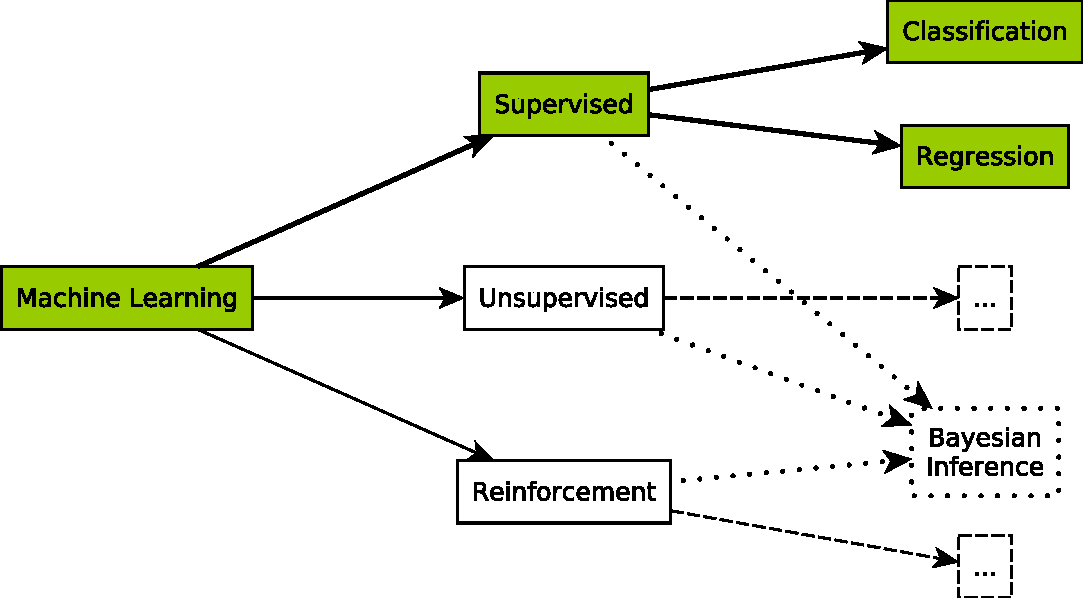
\includegraphics[width=.8\linewidth]{figures/ml-taxonomy.pdf}
    \caption[Taxonomy of ML]{Taxonomy of ML. The second column enumerates the three major families of ML approaches, the third one enumerates the main sorts of tasks affiliated with each family, whereas the fourth one enumerates possible applications for each task}
    \label{fig:ml-taxonomy}
\end{figure}
%
As depicted in \cref{fig:ml-taxonomy}, three major approaches to ML exist.
%
Each approach is characterised by a well-defined pool of tasks, which may, in turn, be applied in wide range of use case scenarios.
%
The three major approaches to learning are: \emph{supervised}, \emph{unsupervised}, and \emph{reinforcement}.
%
They essentially deal with the kind of task $T$ to be learned -- commonly consisting in the estimation of an unknown relation --, and how experience $E$ is provided to the learning algorithm.

In supervised learning, the learning task consists of finding a way to approximate an unknown relation, given a sampling of its items---which constitute the experience.
%
In unsupervised learning, the learning task consists of finding the best relation for a sample of items -- which constitute the experience --, following a given optimality criterion intensionally describing the target relation.
%
In reinforcement learning, the learning task consists of letting an agent estimate optimal plans given the reward it receives whenever it reaches particular goals---constituting the experience.
%
There, a plan can be described as a relation among the possible states of the world, the actions to be performed in those states, and the reward the agents expects to receive from that action.

Such categorisation of learning approaches can be applied to both symbolic and sub-symbolic techniques.
%
Indeed, in this chapter, we provide an overview of learning on a per-representation basis.
%
In particular, in the following sections we summarise the state of the art for what concerns both symbolic and sub-symbolic forms of \emph{supervised} learning.

\section{Sub-Symbolic Supervised Machine Learning}

Since several practical AI problems -- such as image recognition, financial and medical decision support systems -- can be reduced to \emph{supervised} ML -- which can be further grouped in terms of either  \emph{classification} or \emph{regression} problems \cite{twala2010,smlreview-faia160} --, in the reminder of this section we focus on this set of ML problems.

Within the scope of sub-symbolic supervised ML, a \emph{learning algorithm} is commonly exploited to approximate the specific nature and shape of an unknown \emph{prediction} function (or \emph{predictor}) $\pi^*: \mathcal{X} \rightarrow \mathcal{Y}$, mapping data from an input space $\mathcal{X}$ into an output space $\mathcal{Y}$.
%
There, common choices for both $\mathcal{X}$ and $\mathcal{Y}$ are, for instance, the set of vectors, matrices, or tensors of numbers of a given size---hence the sub-symbolic nature of the approach.

An important assumption significantly affecting both the theory and the practice of sub-symbolic supervised learning is that vectors, matrices, or tensors in $\mathcal{X}$ and $\mathcal{Y}$ are of \emph{fixed} size---despite items in $\mathcal{X}$ may have different sizes than the items in $\mathcal{Y}$.
%
Without lack of generality, in what follows we refer to items in $\mathcal{X}$ as $n$-dimensional vectors denoted as $\mathbf{x}$, whereas items in $\mathcal{Y}$ are $m$-dimensional vectors denoted as $\mathbf{y}$---despite matrices or tensors may be suitable choices as well.

To approximate function $\pi^*$, supervised learning assumes a learning \emph{algorithm} is in place.
%
This algorithm computes the approximation by taking into account a number $N$ of \emph{examples} of the form $(\mathbf{x}_i,\mathbf{y}_i)$ such that $\mathbf{x}_i \in X \subset \mathcal{X}$, $\mathbf{y}_i \in Y \subset \mathcal{Y}$, and $|X| \equiv |Y| \equiv N$.
%
There, the set $D = \{ (\mathbf{x}_i,\mathbf{y}_i) \mid \mathbf{x}_i \in X, \mathbf{y}_i \in Y \}$ is called \emph{training} set, and it consists of $(n+m)$-dimensional vectors.
%
The dataset can be considered as the concatenation of two matrices, namely the $N \times n$ matrix of \emph{input} data ($X$) and the $N \times m$ matrix of \emph{expected output} data ($Y$).
%
There, each $\mathbf{x}_i$ represents an instance of the input data for which the expected output value $\mathbf{y}_i \equiv \pi^*(\mathbf{x}_i)$ is known or has already been estimated.
%
Notably, such sorts of ML problems are said to be ``supervised'' \emph{because} the expected outputs $Y$ are available.
%
Furthermore, the function approximation task is called ``regression'' if the components of $Y$ consist of continuous or numerable -- i.e. \emph{infinite} -- values, or ``classification'' problems they consist of categorical -- i.e. \emph{finite} -- values.

Many learning algorithms exist, and they work in quite different ways.
%
However, the general layout of sub-symbolic supervised learning is the same in all cases.
%
The learning algorithm assumes $\pi^*$ to be a function from a given set of functions $\mathcal{H}$ called \emph{hypotheses} space---i.e. $\pi^* \in \mathcal{H}$.
%
In other words, the underlying assumption is that the unknown prediction function $\pi^*$ exists, and it is of the form characterising all functions in $\mathcal{H}$.
%
The algorithm performs an exploration of the \emph{hypotheses} space $\mathcal{H}$ looking for the hypothesis function $\hat{\pi} \in \mathcal{H}$ that better fits the data in $D$---and that, therefore, better approximates $\pi^*$.

The goodness of the fitting among a hypothesis function $\hat{\pi}$ and the data can be assessed via either
%
\begin{inlinelist}
    \item an error function $\varepsilon : \mathcal{Y} \times \mathcal{Y} \rightarrow \mathbb{R}_{\geq 0}$ measuring the discrepancy among the expected outputs in $Y$ and the values attained by applying $\hat{\pi}$ to $X$, or dually,
    \item an adherence function $\rho : \mathcal{Y} \times \mathcal{Y} \rightarrow \mathbb{R}_{\leq 1}$, measuring the similarities among the same values.
\end{inlinelist}
%
For the sake of simplicity, we here consider the best hypothesis $\hat{\pi}$ the one item of $\mathcal{H}$ for which the total error is minimal -- or the total adherence is maximal --, w.r.t. the data in $D$.
%
Therefore, in theory, any sub-symbolic supervised learning process can be abstractly described via any of the following formul\ae{}:
%
$$
\hat{\pi} = \argmin{\pi \in \mathcal{H}}{ \sum_{i=1}^{N} \varepsilon(\mathbf{y}_i,\ \pi(\mathbf{x}_i)) }
\quad \text{or} \quad
\hat{\pi} = \argmax{\pi \in \mathcal{H}}{ \sum_{i=1}^{N} \rho(\mathbf{y}_i,\ \pi(\mathbf{x}_i)) }
$$

\paragraph{Parameters and hyper-parameters}

Exploration of the hypothesis space is what is commonly referred to as ``learning'' or ``training''.
%
Learning algorithms mostly differ for the strategy they follow to perform such exploration, other than the particular hypotheses spaces they support.

A common strategy followed by most learning algorithms leverages on the assumption that the hypothesis space is the set of all functions having the same shape, regulated by a given amount $p$ of \emph{parameters}---namely $\mathcal{H}_\Theta$ where $\Theta \subseteq \mathbb{R}^p$ is space of parameters, enumerated by $\theta$.
%.
Under such assumption, the formulation of supervised learning can be rewritten as the optimisation task of finding the optimal parameters $\theta^*$ among the ones in $\Theta$:
%
$$
\theta^* = \argmin{\theta \in \Theta}{ \sum_{i=1}^{N} \varepsilon(\mathbf{y}_i,\ \pi_\theta(\mathbf{x}_i)) }
\quad \text{or} \quad
\theta^* = \argmax{\theta \in \Theta}{ \sum_{i=1}^{N} \rho(\mathbf{y}_i,\ \pi_\theta(\mathbf{x}_i)) }
$$
%
where $\pi_\theta \in \mathcal{H}_\Theta$ is the particular function using the parameters in $\theta$.

If all functions in $\mathcal{H}_\Theta$, as well as the error (resp. adherence) function $\varepsilon$ (resp. $\rho$), are differentiable w.r.t. $\theta$, then the optimisation task can be tackled via gradient descent (resp. climbing) in the general case---despite better options may exist for particular shapes of the functions in $\mathcal{H}_\Theta$.
%
Such need to rely on differentiable functions of vectors of real numbers is what forces many ML techniques into the sub-symbolic realm.

Notably, a hypothesis space is commonly generated by a particular assignment of a number $q$ of \emph{hyper-parameters} $\omega \in \mathbb{R}^q$.
%
Each particular value of $\omega$ corresponds to a particular parameters space $\Theta$, and therefore to a particular hypothesis space $\mathcal{H}_\Theta^\omega$.
%
The hypothesis space may consist for instance of the set of all polynomials of $a$ variables whose degree is $b$.
%
That would imply the corresponding parameters space to comprehend all possible vectors having $\binom{b}{a}$ components.
%
So, if $a = b = 1$, then $\mathcal{H}_\Theta^\omega$ is the set of all possible straight lines on a plane, i.e. polynomials parametrised by $\theta_1$ and $\theta_2$.
%
For $a = 1$ and $b = 2$, $\mathcal{H}_\Theta^\omega$ corresponds to the set of all possible parabolas on a plane, i.e. polynomials parametrised by $\theta_1$ and $\theta_2$ and $\theta_3$.
%
A similar example may be built upon polynomials of 2 variables, and so on.

The difference among parameters and \emph{hyper-}parameters is very important in practice.
%
In fact, while parameters are \emph{automatically} computed by the learning algorithm, hyper-parameters are not.
%
They may be either guessed or estimated by trial-and-error by data scientists---hence representing a bottleneck in the automatisation of learning.

%\note{About generalisation: the bias-variance trade-off?} % maybe out of topic

\subsection{Overview on learning algorithms}

%\note{
%    Comments on existing algorithms and their relevant aspects?
%    Let's distinguish among parametric and non-parametric algorithms.
%    Let's distinguish among regression and classification algorithms, with a focus on regression as classification can be reduced to regression.
%    Focus on gradient descent, back-propagation and deep learning.
%}

Depending on the predictor family of choice, the nature of the admissible hypotheses spaces and learning algorithms may vary dramatically, as well as the predictive performance of the target predictor, and the whole efficiency of learning.

In the literature of machine learning, statistical learning, and data mining, a plethora of learning algorithms have been proposed along the years.
%
Because of the ``no free lunch'' (NFL) theorem \cite{DolpertM97}, however, no algorithm is guaranteed to outperform the others in all possible scenarios.
%
For this reason, the literature and the practice of data science keeps leveraging on algorithms and methods whose first proposal was published decades ago.
%
Most notable algorithms include for instance (deep) neural networks, decision trees, (generalised) linear models, nearest neighbours, support vector machines (SVM), random forests, and many others.

These algorithms can be categorised in several ways, for instance depending on
%
\begin{inlinelist}
    \item the supervised learning task they support (classification vs. regression),
    \item on when they consume data (lazy vs. eager),
    \item or on the underlying strategy adopted for learning (e.g. gradient descent, least squares optimisation), etc.
\end{inlinelist}

Some learning algorithms (e.g. neural networks) target regression problems, whereas others (e.g. SVM) target classification problems.
%
Similarly, some target multi-dimensional outputs ($\mathbf{y} \in \mathbb{R}^m$), whereas others target mono-dimensional outputs ($m = 1$).
%
Regressors are considered as the most general case, as other learning tasks can usually be defined in terms of mono-dimensional regression.
%
Binary classifiers, for instance, can be treated as mono-dimensional regressors where admissible outputs lay in the interval $[0, 1]$, while multi-class (resp. multi-dimensional) classifiers (resp. regressors) can be treated as ensembles of multiple binary classifiers (resp. regressors).

% briefly explain the eager-lazy dicotomy
The eager--lazy dichotomy relates to operational aspects of learning, and, in particular, to \emph{when} training data is actually processed.
%
This, in turn, affects the computational time required in the training and inference phases---i.e. when the predictor is exploited to draw predictions.
%
In principle, the training phase of \emph{lazy} predictors (e.g. nearest neighbours) is trivial and no data needs to be processed as training data is mostly processed in the inference phase.
%
This makes the training phase quicker, at the expense of a slower inference phase.
%
To mitigate this issue, in practice, indexing or grouping of training data may be exploited in the training phase, with the purpose of speeding up the inference phase.
%
Conversely, \emph{eager} predictors (e.g. linear models, neural networks, and virtually any other method mentioned so far) come with a full-fledged learning phase, where the unknown function binding input and outputs is approximated from training data.
%
There, the learning phase carries the higher computational effort, and the inference phase is quick.
%
In the reminder of this section, we focus on eager predictors as they actually produce an internal representation of data during their learning phase, which is the starting point of relevant discussion carried out in \cref{chap:explaining}.

% discuss about GD-based approaces
Finally, the learning strategy is inherently bound to the predictor family of choice.
%
Neural networks, for instance, are trained via back-propagation \cite{Rumelhart1986} -- a particular case of stochastic gradient descent (SDG, \cite{enwiki:SGD}), tailored on NN --, generalised linear models via Gauss' least squares method, decision trees via CART \cite{breiman1984classification}, etc.
%
Despite all such algorithms may appear interchangeable in principle -- because of the NFL theorem --, their malleability is very different in practice.
%
For instance, the least squares method involves inverting matrices of order $N$ -- where $N$ is the amount of available examples in the training set --, making the computational complexity of learning more than quadratic in time.
%
Furthermore, in practice, convergence of the method is not guaranteed in the general case, while it is for generalised linear models---hence why it is not adopted elsewhere.
%
Thus, learning by least squares optimisation may become impractical for big datasets or for predictor families outside the scope of generalised linear models.
%
Conversely, the SGD method involves arbitrarily-sized subsets of the dataset (a.k.a. batches) to be processed a limited (i.e. controllable) amount of times.
%
Hence, the complexity of SGD can be finely controlled and adapted to the computational resources at hand---e.g. by making the learning process incremental, and by avoiding all data to be loaded in memory.
%
Furthermore, SGD can be applied to several sorts of predictor families (there including neural networks and generalised linear models), as it only requires the target function to be differentiable w.r.t. its parameters.
%
For all these reasons, despite the lack of optimality guarantees, SGD is considered as very effective, scalable, and malleable in practice, hence why it is extensively exploited in the modern data science applications.

In the reminder of this thesis, we focus on two particular families of predictors -- namely, decision trees and neural networks --, and their respective learning methods---i.e. the CART \cite{breiman1984classification} and back-propagation \cite{Rumelhart1986} algorithms.
%
Notably, decision tree are relevant because of their user friendliness, whereas neural networks are relevant because of their predictive performance and flexibility.

\paragraph{Decision Trees}

\begin{figure}
    \centering
    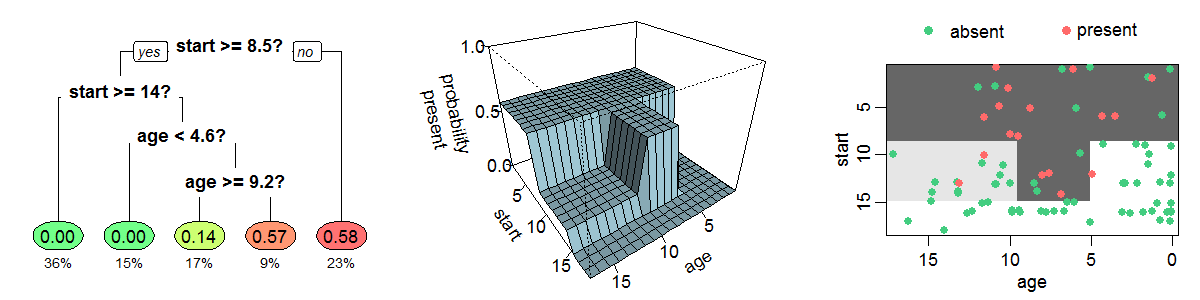
\includegraphics[width=\linewidth]{figures/dt-kyphosis.png}
    \caption[An example decision tree estimating the probability of kyphosis after spinal surgery]{An example decision tree estimating the probability of kyphosis after spinal surgery, given the \emph{age} of the patient and the vertebra at which surgery was \emph{start}ed \cite{wiki:dt-learning}. Notice that each decision tree subtends a partition of the input space, and that the tree itself provides an intelligible representation of \emph{how} predictions are attained}
    \label{fig:dt-example}
\end{figure}

Decision trees (DT) are particular sorts of predictors supporting both classification and regression tasks.
%
In their learning phase, the input space is recursively \emph{partitioned} through a number of splits (a.k.a. \emph{decisions}) based on the input data $X$, in such a way that the prediction in each partition is constant, and the error w.r.t.\ the expected outputs $Y$ is minimal, while keeping the total amount of partitions low as well.
%
The whole procedure then synthesises a number of \emph{hierarchical} decision rules to be followed whenever the prediction corresponding to any $x \in \mathcal{X}$ must be computed.
%
In the inference phase, decision rules are orderly evaluated from the root to some leaf, in order to select the portion of the input space  $\mathcal{X}$ containing $x$.
%
As each leaf corresponds to a single portion of the input space, the whole procedure results in a single prediction for each $x$.

Differently from other families of predictors, the peculiarity of decision trees lays in the particular outcome of the learning process -- namely, the \emph{tree} of decision rules -- which is naturally intelligible for humans and graphically representable in 2D charts.
%
As further discussed in the reminder of this thesis, this property is of paramount importance whenever the inner operation of an automatic predictor must be interpreted by a human being.


%Without affecting generality, we focus on the case of mono-dimensional classification -- thus we write $y$ instead of $\mathbf{y}$ --, since other cases can be easily reduced to this one.
%%
%We further assume the input space $\mathcal{X}$ is $N$-dimensional, and let $n_j$ be the meta-variable representing the name of the $j^{th}$ dimension of $\mathcal{X}$.
%
%Under such hypotheses, a DT predictor $p_T \in \mathcal{P}_{dt}$ assumes a \emph{binary} tree $T$ exists such that each node is either
%%
%\begin{itemize}
%    \item a \emph{leaf}, carrying and representing a prediction, i.e. and assignment for $y$,
%    \item an \emph{internal} node, carrying and representing a \emph{decision}, i.e. a formula in the form $(n_j \leq c)$---where $c$ is a constant \emph{threshold} chosen by the learning algorithm.
%\end{itemize}
%%
%Each node $\nu$ inherits a partition $X_\nu \subseteq X$ of the original input data, from its parent.
%%
%Since the root node $\nu_0$ has no parent, it is assigned to the whole set of input data---i.e. $X_{\nu_0} \equiv X$.
%%
%The decision carried by each internal node splits its $X_\nu$ into two disjoint parts -- $X^L_\nu$ and $X_\nu^R$ -- along the $j^{th}$ dimension of $\mathcal{X}$.
%%
%In particular, $X_\nu^L $ contains all the residual $x_i \in X_\nu$ such that $(x_i^j \leq c_\nu)$ -- which are inherited by $\nu$ left child --, whereas $X_\nu^R$ contains all the residual $x_i \in X_\nu$ such that $x_i^j > c_\nu$---which are inherited by  by $\nu$ right child.
%%
%A leaf node $l$ is created whenever a sequence of splits (i.e., a path from the tree root to the leaf parent) leads to a partition $X_l$ which is (almost) \emph{pure}---roughly, meaning that $X_l$ (mostly) contains input data $x_i$ for which the expected output is the same $y_l$.
%%
%In this case, we say that the prediction carried by $l$ is $y_l$.
%%
%Assuming such a tree $T$ exists, in order to classify some input data $\mathbf{x} \in \mathcal{X}$, the predictor $p_T$ simply navigates the path $P = (\nu_0, \nu_1, \nu_2, \ldots, l)$ of $T$ such that all decisions $\nu_k$ are matched by $\mathbf{x}$, then it outputs $y_l$.

\paragraph{Neural Networks}

Neural networks (NN) are biologically-inspired computational models, made of several elementary units (neurons) interconnected into a graph (commonly, \emph{directed} and \emph{acyclic}, a.k.a. DAG) via \emph{weighted} synapses.
%
Accordingly, the most relevant aspects of NN concern the inner functioning of neurons and the particular architecture of their interconnection.

Neurons are very simple numeric computational units.
%
They accept $n$ scalar inputs $(x_1, \ldots, x_n) = \mathbf{x} \in \mathbb{R}^n$ weighted by as many scalar weights $(w_1, \ldots, w_n) = \mathbf{w} \in \mathbb{R}^n$, and they process their linear combination $\mathbf{x} \cdot \mathbf{w}$ via an activation function \cite{enwiki:ActivationFunctions} $\sigma : \mathbb{R} \mapsto \mathbb{R}$, producing a scalar output $y = \sigma(\mathbf{x} \cdot \mathbf{w})$, as depicted in \cref{fig:neuron}.
%
\begin{figure}
    \centering
    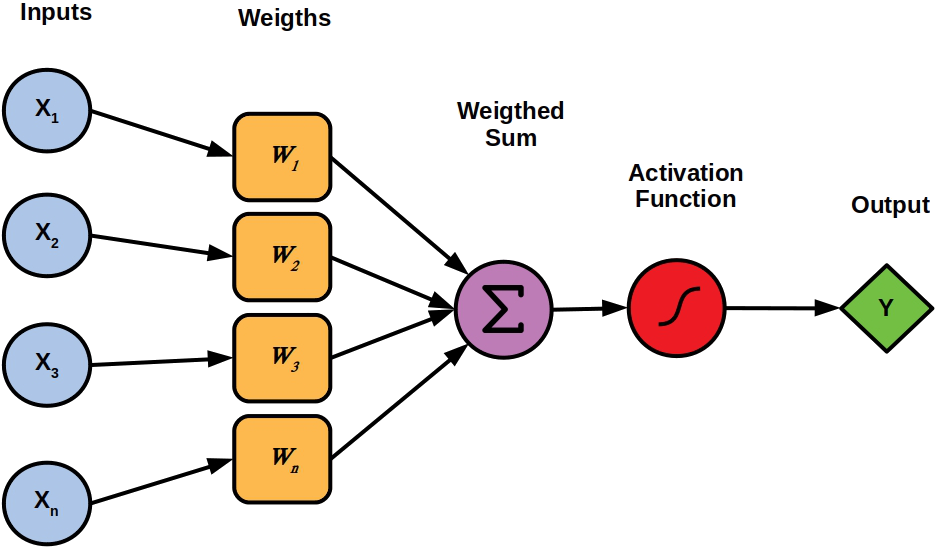
\includegraphics[width=.6\linewidth]{figures/neuron.png}
    \caption{General structure of neural units in neural networks}
    \label{fig:neuron}
\end{figure}
%
The output of a neuron may become the input of many others, possibly forming \emph{networks} of neurons having arbitrary topologies.
%
These network may be fed with any numeric information encoded as vectors of real numbers by simply letting a number of neurons produce constant outputs.

While virtually all topologies are admissible for NN, not all are convenient.
%
A number of convenient \emph{architectures} -- roughly, patterns of well-studied topologies -- have been proposed into the literature \cite{VanVeenL2019} to serve disparate purposes---far beyond the scope of supervised machine learning.
%
\Cref{fig:nn-architectures} overviews the current state of the art of NN architectures.
%
\begin{figure}
    \centering
    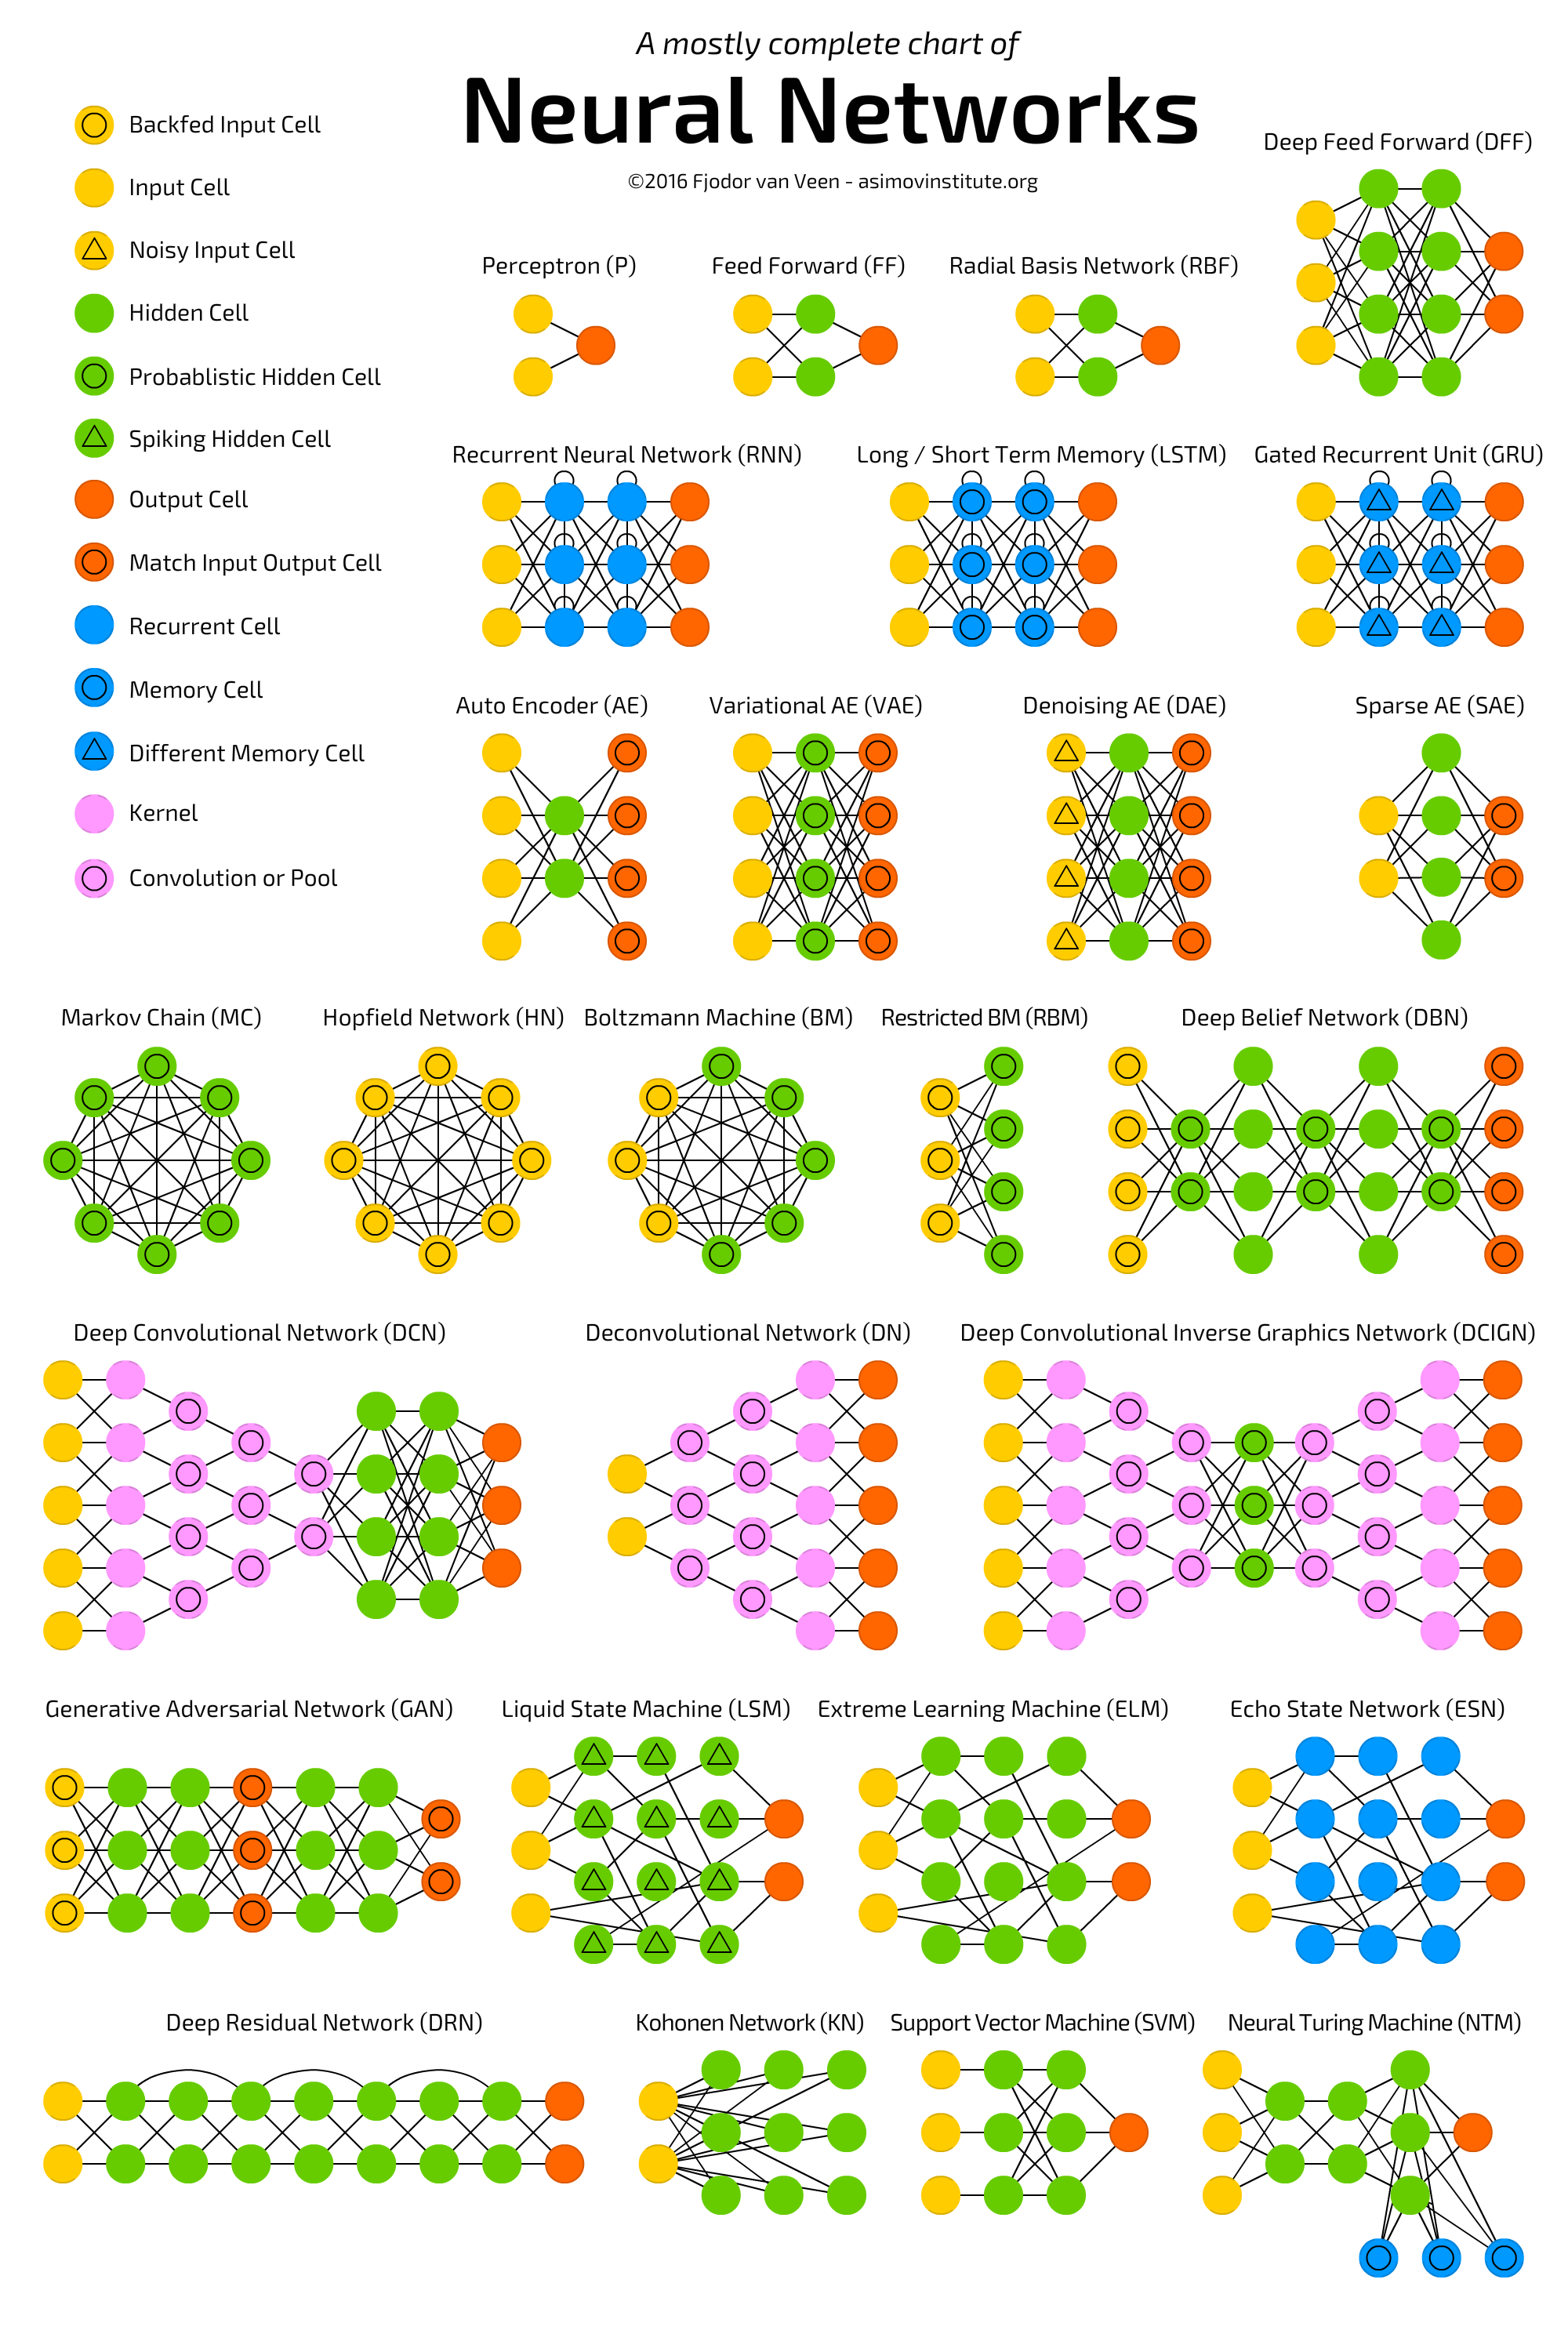
\includegraphics[width=.8\linewidth]{figures/neural-network-architectures.png}
    \caption[Admissible architectures for neural networks]{Admissible architectures for neural networks \cite{VanVeenL2019}}
    \label{fig:nn-architectures}
\end{figure}

NN can be \emph{trained} on numeric data via stochastic gradient descent and exploited into both supervised and unsupervised learning tasks such as classification, regression, and anomaly detection, depending on the particular architecture of choice.
%
More precisely, while the training \emph{automatically} sets up the weights of each neuron's ingoing synapses, the overall topology of the network is not allowed to vary.
%
It is rather assumed to be \emph{manually} engineered by data scientists.

Most common NN architectures are feed-forward, meaning that neurons are organised in successive \emph{layers}, in such a way that neurons from layer $i$ can only accept ingoing synapses from neurons of layers $j < i$.
%
The first layer is considered the input layer, which is used to \emph{feed} the whole network, while the last one is the output layer, where prediction are drawn.
%
In architectures of these kinds, inference lets information flow from the input to the output layers -- assuming the weights of synapses are fixed --, while training lets information flow from the output to the input layers---provoking the variation of weights to minimise the prediction error of the overall network.

The recent success of deep learning \cite{GoodfellowBC2016} has proved the flexibility and the predictive performance of \emph{deep} neural networks (DNN).
%
`Deep' here refers to the large amount of (possibly \emph{convolutional}) layers.
%
In other words, DNN can learn how to apply cascades of convolutional operations to the input data.
%
Convolutions let the network spot relevant features into the input data, at possibly different scales.
%
Hence why DNN are good at solving complex pattern-recognition tasks, such as in computer vision or speech recognition.
%
Unfortunately, however, unprecedented predictive performances of DNN come at the cost of their increased internal complexity and greater data greediness.

\section{Symbolic Supervised Learning}
\label{sec:symbolic-supervised-learning}

Within the realm of symbolic AI, supervised ML commonly refers to either \emph{inductive logic programming} (ILP) \cite{Muggleton91} or \emph{statistical relational learning} (SRL) \cite{DeRaedt2010}, despite the overlap among the two disciplines is wide.

In both cases, learning consists of approximating an unknown \emph{intensional} representation $H^*$ for a number of positive examples $E^+$, possibly leveraging on
%
\begin{itemize}
    \item some prior knowledge base $B$, carrying the so-called \emph{background knowledge} about the domain at hand;
    \item a number of \emph{negative} examples $E^-$;
    \item a \emph{language bias} $C$, constraining the admissible shapes for the representation to-be-learned.
\end{itemize}
%
In the general case, $H^*$, $E^+$, $E^-$, and $B$ are knowledge bases, possibly involving several definite clauses (i.e. either rules or facts), while the shape of $C$ really depends on the particular learning approach at hand.
%
Of course, there may be cases where $E^-$, $B$ or $C$ are not required, and therefore considered as empty sets.

The main difference among ILP and SLR lays in the particular language used for knowledge representation.
%
While in ILP knowledge bases simply consist of bare definite clauses, SRL leverages on a superset of Horn Logic called LPAD (Logic Programs with Annotated Disjunctions) \cite{VennekensVB04}, where definite clauses are enriched with probability values.

According to the SLR nomenclature of \cite{DeRaedt2010} -- where a unifying model generalising ILP and SLR is proposed --, there are two relevant problems which lay under the symbolic supervised learning umbrella, namely:
%
\begin{description}
    \item[parameters learning] where $H$ consists of a given LPAD theory, where the shape of facts and rules is known, while their probabilities are not, and learning aims at simply estimating those probabilities

    \item[structure learning] where $H$ is completely unknown, and the whole shape of facts and rules therein contained must be computed, possibly along with their corresponding probabilities
\end{description}

In both cases, learning can be defined as an optimisation problem aimed at approximating $H^*$ by search for the best KB $\hat{H}$ into a hypothesis space $\mathcal{H}_{B,C}$, defined by applying all possible combinations of clauses in $B$, as dictated by $C$.
%
There, each KB $H \in \mathcal{H}_{B,C}$ consists of a number of definite clauses defining the $n$-ary relation $h$, possibly leveraging on the relations defined in $B$, and satisfying the suggestions/constraints expressed by $C$.
%
In other words, they consist of KB intensionally defining $h$ via rules of the form:
%
\begin{equation*}
    \psi :: h(X_1,\ \ldots,\ X_n) \leftarrow f(\bar{X}),\ f'(\bar{X}'),\ f''(\bar{X}''),\ \ldots
\end{equation*}
%
where $\psi$ denotes an optional probability value,  while $\bar{X}, \bar{X}', \bar{X}'', \ldots$ are tuples involving one or more head variables (i.e., $X_1, \ldots, X_n$), and $f, f', f'', \ldots$ are either predicates defined in $B$ or combinations of those predicates, attained by following the suggestions/constraints contained in $C$.
%
Similarly, $E^+$ (resp. $E^-$) consists of facts of the form $h/n$, extensionally defining known (resp. invalid) items of the $n$-aray relation $h$, and possibly labelled with probabilities.

Analogously to the sub-symbolic case, symbolic supervised learning leverages upon some adherence function $\rho$, aimed at measuring the adherence of some hypothesis KB $H \in \mathcal{H}_{B,C}$ w.r.t. either $E^+$ or $E^-$.
%
For instance, in SRL, $\rho$ is commonly modelled probabilistically:
%
\begin{equation*}
    \rho(H, E, B) = \sum_{e \in E} \mathbb{P}(e \mid H, B)
\end{equation*}
%
where $\mathbb{P}(\cdot \mid \cdot)$ denotes the conditional probability operator.
%
Conversely, in ILP, $\rho$ is modelled in terms of logic inference\footnotemark:
%
\begin{equation*}
    \rho(H, E, B) = \sum_{e \in E} \rho(H, e, B)
    \quad \text{and} \quad
    \rho(H, e, B) = \begin{cases}
        1 & \text{if} ~ H, B \models e
        \\
        0 & \text{otherwise}
    \end{cases}
\end{equation*}
%
\footnotetext{
    This aspect is better discussed in \cref{chap:reasoning}.
    %
    Within the scope of this chapter, the notation $K \models \phi$, where $K$ is a knowledge base and $\phi$ is a logic formula, can simply be read as ``$\phi$ can be inferred from $K$ via some inference procedure''.
}
%
Under such hypothesis, symbolic supervised learning can be defined as \cite{DeRaedt2010} the optimisation task aimed at finding the hypothesis which adheres to as much positive examples as possible, while adhering to no negative example at all:
%
\begin{equation}
    \hat{H} = \argmax{H \in \mathcal{H}_{B,C} ~ \text{s.t.} ~ \rho(H, E^-, B) = 0}{\rho(H, E^+, B)}
\end{equation}

Parameter and structure learning differ for the actual way the search is performed, other than for the actual object of search.
%
In parameter learning, algorithms can assume the shape of (facts and rules in) $\hat{H}$ to be given (and fixed), and therefore focus on the mere estimation of probabilities.
%
Conversely, in structure learning, algorithms must also consider the many possible shapes $\hat{H}$ may have.
%
This includes all possible combinations of all relations possibly defined in $B$.
%
Assuming, for instance, that $B$ intensionally defines $r$ relations $f_1, \ldots, f_r$, whose arity is at least $a$, and that the target relation is $h$, whose arity is $n$.
%
Under such hypothesis, rules in $H$ should be of the form:
%
\begin{equation*}
    h(X_1,\ \ldots,\ X_n) \leftarrow \ldots
\end{equation*}
%
where the body of the rule may contain as many predicates as in any possible permutation of any possible subset of $\{ f_1, \ldots, f_r \}$.
%
There, each possible $a$-ary relation could be written as a predicate involving some disposition of $a$ variables from the set $\{ X_1, \ldots, X_n \}$.
%
In other words, the search space for structure learning is \emph{huge} and definitely impossible to explore in useful time, unless in trivial cases.
%
To complicate the matter, differently from the sub-symbolic case, the search space is not even continuous---meaning that gradient based approaches cannot be applied.

To mitigate such issues -- and to reduce the search space --, the ILP community leverages on smart choices of the linguistic bias $C$.
%
The general purpose of the linguistic bias is to constrain the particular way relations from $B$ can be combined in $H$.
%
This can come in different shapes and flavours, depending on the particular ILP method in place.

Consider for instance the case of an ILP problem aimed at learning the positive example $grandparent(\functor{abraham}, \functor{jacob})$, given the background knowledge containing a number of facts expressing parenthood facts of the form $parent(\functor{p}, \functor{p}')$, describing Abraham's family tree---as in \cref{eq:abraham-family-tree}.
%
There, the meta-rule \ref{eq:meta-rule-example} may suggest the correct identification of the target rule -- namely, $grandparent(X, Y) \leftarrow parent(X, Z), parent(Z, Y)$ -- via the variable assignment $\{ \textsf{P} \mapsto grandparent, \textsf{Q} \mapsto parent, \textsf{R} \mapsto parent \}$.

It is worth to be noted how the language bias $C$ plays, in symbolic supervised learning, the same role played by hyper-parameters in sub-symbolic supervised learning.
%
In both cases, \emph{automated} learning relies on some prior knowledge, which must be handcrafted by data scientists.
%
In fact, similarly to sub-symbolic approaches, some mechanism is needed to let humans control either the complexity or learning or the dimension of the search space.
%
In the particular case of symbolic supervised learning, that mechanism is the language bias.

\subsection{Overview on learning algorithms}

Here we summarize the most relevant sorts of algorithms supporting symbolic supervised learning.
%
In particular, we focus on algorithms aimed at learning either the structure or the parameters of logic programs.
%
We discuss approaches targeting structure learning first.
%
Then, we introduce approaches for parameter learning---which commonly require the structure to be given.

\subsubsection{Structure Learning}

%\note{
%    Intuition behind the functioning of the algorithms.
%    Bottom up or top down approaches in ILP.
%    Mention main approaches: relatively least general generalisation, reverse entailment, bottom clause generalisation, meta-interpretative learning.
%    Mention major algorithms developed in this field.
%}

Structure learning of logic programs is commonly attained via some ILP algorithm.
%
A nice and up-to-date survey of ILP is provided by \cite{CropperD2020}.
%
Here, we just provide an overview and some references.

Generally speaking, ILP algorithms aim to construct a good -- i.e. \emph{sufficiently} general -- theory $H^*$ entailing all positive examples in $E^+$ and no negative one from $E^-$.
%
Clauses from the theory under construction may leverage upon one or more clauses from the background knowledge $B$.
%
In other words, ILP algorithms exploit automated inductive reasoning to produce novel symbolic knowledge -- possibly leveraging on previously available symbolic knowledge -- out of positive and negative symbolic examples.


Notably, the notion of ``\emph{sufficiently} general theory'' is quite subtle in this context.
%
Roughly speaking, a \emph{general} theory should contain one or more non-ground clauses, from which the positive examples could be attained via variables substitutions or via deduction.
%
Despite the expected result of any ILP algorithm is certainly a \emph{general} theory from which all the positive examples can be inferred, looking for the \emph{most} -- or \emph{least} -- possible general rule is likely a mistake.
%
In other words, as for sub-symbolic ML, generalising too much is as wrong as generalising too little---i.e. drawing rules which are too specific.
%
In fact, any inductive inference process may lead to the construction of too general conclusions which do not hold in the real world.
%
To prevent this issue, ILP algorithms commonly include some stopping criterion aimed at avoiding both excessive generalization and excessive generalization.

From a very high-level perspective, ILP algorithms can be categorized w.r.t. the strategy they follow in constructing the target theory.
%
Top-down algorithms start from a very general theory and they progressively specialise it, until reaching the most general theory among the most specific ones.
%
Conversely, bottom-up algorithms follow the inverse path, starting from a very specific theory and then progressively generalising it, until reaching the most general theory among the most specific ones.

In practice, four major approaches have been proposed into the ILP literature -- namely, relative least-general generalization, inverse entailment, bottom-clause propositionalisation, and meta-interpretative learning --, and most algorithms proposed so far rely on some of them.

\paragraph{Relative least-general generalization (RLGG)}

RLGG \cite{Plotkin1971} is a basic mechanism to be exploited in a bottom-up induction strategy.
%
It assumes both the background knowledge and the examples to be ground.
%
Under this assumption, it subtends a lattice where vertices represent clauses and arcs represent instances of a subsumption relation.
%
Such clauses attained by
%
\begin{inlinelist}
    \item combining the literals from the positive examples among each other and with the literals of the clauses in the background knowledge, and by
    \item replacing common constant terms with variables, accordingly.
\end{inlinelist}

To perform induction, the resulting lattice should then be explored looking for the best RLGG, i.e. the one covering the more positive examples, while not covering any negative example.
%
Unfortunately, however, the lattice may be very large or even infinite, thus further sub-strategies should be in place to
%
%The resulting clause may be very large -- or even infinite --, so further sub-strategies should be in place to
%
\begin{inlinelist}
    \item \emph{lazily} generate and explore the lattice,
    \item prevent it from exploding in size, and
    \item prune the lattice as quickly and as much as possible.
\end{inlinelist}

Golem \cite{MuggletonF1990} is an algorithm and former software system exploiting RLGG in practice.
%
In a seek for tractability, Golem puts some constraints on the amount and the position of variables in the literal composition phase.
%
It starts by constructing a very large clause using positive examples, and, after a number of generalization steps where constant terms are replaced by variables, the clause reaches its final form as the outcome of the induction process.
%
Behind the scenes, negative examples are exploited to prune the resulting clause.

\paragraph{Inverse entailment (IE)}

IE \cite{Muggleton95} is another basic mechanism supporting the induction of logic clauses following a bottom-up strategy.
%
Like RLGG, IE subtends a generality lattice of clauses to be explored.
%
However, differently than RLGG, IE may generalize a clause via \emph{predicate invention}---i.e. by generating a bare new predicate, different than the ones in the examples and background knowledge.
%
Thanks to predicate invention, IE can lead to the induction of elegant and concise theories composed by one or more interrelated clauses.

While the IE mechanism itself is straightforward, it simply moves the complexity into predicate invention.
%
Indeed, linguistic bias in the form of suggestions and constraints for the predicate invention sub-procedure must be commonly provided by the users.

Progol, for instance, is likely the first and most relevant ILP system leveraging upon IE.
%
It has been proposed by the same paper \cite{Muggleton95}. %, and it exploits a mixed strategy which can be considered both top-down and bottom-up.
%
Notably, it requires the user to provide ``mode declarations'' via an ad-hoc syntax, to define and constrain predicate invention.
%
This is required to construct the ``bottom clause'', i.e.  most-specific clause that explains an example.
%
Progol then relies upon an A$^*$-like heuristic search -- exploiting a compression score as the heuristic function -- to generalise the clause to make it cover as much examples as possible.
%
%The procedure is repeated as
%
%Behind the scenes, Progol exploits an A$^*$-like heuristic algorithm to

\paragraph{Bottom-clause propositionalisation (BCP)}

In the BCP approach \cite{Franca2014}, bottom clauses attained by generalising the examples are \emph{propositionalised} -- i.e. brought into attribute-value form -- by using the set of all body literals that occur in them and in the background knowledge's clauses as possible attributes.
%
This reduces the logic knowledge into an extensional dataset of fixed size, which can be used to fed sub-symbolic predictors.

C-IL$^2$P \cite{GarcezZ99} and CILP++ \cite{Franca2014} are notable examples of systems perform ILP by relying on BCP and by constructing a neural network behind the scenes.
%
In these systems, neural networks are constructed to reflect the background knowledge's and the examples' literals into its structure.
%
The neural network is then trained, and an induced clause is then reverse-engineered from the network's weights.

\paragraph{Meta-interpretative learning (MIL)}

MIL \cite{MuggletonLPT14} is a modern approach leveraging on the meta-programming capabilities of logic solvers (cf. \cref{chap:reasoning})---and in particular Prolog ones.
%
Following the MIL approach, ILP is conceived as a higher-order logic task where a logic program (the meta-interpreter) dynamically constructs another logic program (the induced theory) via meta-programming.

There, the linguistic bias consists of a library of higher-order rules (a.k.a. meta-rules), which define the admissible ways the predicates from the examples and the background knowledge may be combined.
%
In particular, a meta-rule is a rule involving higher-order variables enumerating over predicate symbols, such as:
%
\begin{equation}\label{eq:meta-rule-example}
    \textsf{P}(A,\ B) \leftarrow \textsf{Q}(A,\ C),\ \textsf{R}(C,\ B)
\end{equation}
%
where uppercase, sans-serif letters $\textsf{P}, \textsf{Q}, \textsf{R}$ denote higher-order variables, while $A, B, C$ are ordinary variables; and the whole formula allows an induction algorithm to \emph{invent} \cite{MuggletonB88} some binary predicate $\textsf{P}$ by combinations of two binary predicates $\textsf{Q}$ and $\textsf{R}$.

Metagol \cite{MuggletonLT15} is the most prominent example of a system following the MIL approach.
%
It follows a bottom-strategy starting from the positive examples and using meta-rules to guide the generalization process.
%
After generalising all the examples, Metagol checks the consistency of the induced theory against the negative examples.
%
Alternative hypotheses may be explored by the meta-interpreter following the underlying solver's semantics---e.g. backtracking in the case of Prolog.

\subsubsection{Parameter Learning}
\label{ssec:parameter-learning}

Parameter learning is commonly achieved via probabilistic logic programming (PLP).
%
The history of PLP starts with the seminal work of \cite{ng1992probabilistic}, and a nice and up-to-date survey is provided by \cite{riguzzi2018}.

In PLP, theories may contain facts or rules enriched with probabilities, which may, in turn, be queried by the users to investigate not only which statements are true or not, but also under which probability.
%
To support this behaviour, probabilistic solvers leverage ad-hoc resolution strategies explicitly taking probabilities into account.
%
PLP systems may also support the computation of probabilities in presence of data.
%
These features make them ideal to deal with uncertainty and the complex phenomena of the physical world.
%
It is thus unsurprising that Bayesian and data-driven AI, other than cyber physical systems (CPS), are among the areas which would benefit the most from the development of robust and interoperable PLP technologies.

A variety of research contributions exploring the field of PLP exist in the logic programming literature.
%
Proposals often differ for their semantics or syntaxes, or for the way they perform probabilistic reasoning \cite{fierens-2015,kimmig2011implementation,de-raedt-2007,riguzzi-swift-2011}.

Roughly speaking, semantics are concerned with endowing probabilistic programs with meaning.
%
Sato's distribution semantics (DS) \cite{sato1995,sato-1997} is one of the most prominent approaches for the combination of logic programming and probability theory.
%
There, a probabilistic logic program is interpreted as a concise description of many possible worlds, and the probabilities of queries are solved by summing up their probability in each possible world.

Languages adhering to the distribution semantics may in turn differ in how they represent clauses, and their probabilities.
%
A successful approach in this context is LPAD (Logic Programs with Annotated Disjunctions) \cite{VennekensVB04}, where clauses admit disjunctions of atoms in their heads, and each atom is labelled with a probability value.
%
In other words, LPAD is a special notation supporting the definition of non-binary probabilistic distributions over clauses and facts.
%
However, in practice, probabilistic logic programs may support a certain \emph{evidence} \cite{horwich2016probability} to be provided via unannotated fact/rules which are known to be true, even though they may be defined over some probability distribution.

Finally, concerning probabilistic reasoning, PLP generally supports reasoning tasks (cf. \cref{chap:reasoning}), and each of them has been richly documented in the literature \cite{RaedtK15}.
%
Broadly speaking, options range from exact to approximate---the former being more precise and computationally demanding, while the latter being more affordable at the price of lower precision.
%
%In the remainder of this chapter we focus on exact methods only.
%
In any case, a common strategy is to rely upon knowledge compilation \cite{darwiche2002knowledge} to make probabilistic reasoning efficient---i.e., by transforming logic formul\ae{} into simpler (more tractable) forms.
%
Binary decision diagrams (BDD) \cite{akers1978binary,lovato-2014} and their variants/extensions are commonly exploited to serve this purpose \cite{bellodi2013expectation,vlasselaer2014compiling}.

\section{Symbolic vs. Sub-Symbolic Learning}

Symbolic and sub-symbolic approaches to supervised learning share similar formulations, despite the corresponding methods and algorithms operate in quite different ways.
%
Both formulations deal with optimisation problems aimed at iteratively constructing an algorithm mimicking an unknown relation/function in the best possible way, leveraging on a number of examples.
%
However, because of their nature and the inherent way they represent knowledge, both approaches come with pros and cons.
%
Here we focus, on their flexibility, maturity, data and computational efficiency, degree of automation, and validation.

\paragraph{Flexibility and maturity}

For what concerns flexibility, symbolic approaches produce more flexible outcomes, whereas sub-symbolic approaches are characterised by more flexible learning processes.

\subparagraph{Outcomes}

Focussing on symbolic approaches, flexibility lays in the shape of the expected outcomes, which is a direct effect of the particular choice of symbols for KR.
%
``Symbolic'' here implies that knowledge is represented via logic clauses, which in turn pave the way towards learning intensional \emph{relations}---possibly taking some prior (background) knowledge into account.
%
Indeed, representing the target of knowledge in the form of relations expressed by logic formul\ae{} comes with two major advantages---namely bi-directionality and re-usability.

First, relations are \emph{bi-directional}, meaning that any argument of the relation can be considered either an input or an output, depending on the situation at hand.
%
So, for instance, if an agent is capable of learning the clauses expressing the $grandparent/2$ relation -- cf. \cref{eq:abraham-family-tree} --, then it acquires a lot of relevant information, namely:
%
\begin{inlinelist}
    \item an explicit, generic representation of \emph{how} the relation can be tested among any two entities $X$ and $Y$,
    \item a way to compute all the grand-children of any given grand-parent $\functor{p}$ -- i.e. $grandparent(\functor{p}, Y)$ --, and
    \item a way to compute all the grand-parents of any given grand-child $\functor{c}$---i.e. $grandparent(X, \functor{c})$.
\end{inlinelist}

Second, relations are \emph{re-usable} (w.r.t. a learning process), meaning that learned relations can be used as prior knowledge in any sub-sequent learning process, as both the inputs and outputs of any symbolic learning process are represented in the same form---namely, logic clauses.
%
This in turn paves the way towards the definition of learning \emph{cycles} where a learning algorithm is executed several times and the knowledge acquired after each round is included in the background knowledge of successive rounds.

Conversely, sub-symbolic approaches aim to learn \emph{functions}, rather than relations.
%
The learned functions are generally \emph{mono-directional} -- in the sense that they are not (easily) invertible -- and extensional.
%
Consider for instance the case of a neural network aimed at classifying images of animals.
%
It may easily discriminate among dogs and cats (i.e. compute the classification, given an input), yet it may hardly generate admissible images of neither dogs or cats (i.e. compute an input, given a class)\footnotemark.

\footnotetext{Generative Adversarial Neural Networks \cite{GoodfellowPMXWOCB14} may be used whenever bi-directionality is needed, yet that essentially implies training two networks: one \emph{classifier} and one \emph{generator} of data, where the former can only classify, and the latter can only generate data}

\subparagraph{Processes}

Focussing on sub-symbolic approaches, flexibility lays in the variety of methods to approximate the target function.
%
Such variety is once again the result of the particular choice of arrays of numbers for KR.
%
In fact, this choice enables the pervasive exploitation of mathematical operations as the basic bricks of sub-symbolic processing. %learning and computing.
%
These include basic algebraic operators (sum, product, etc.), as well as statistical (mean, variance, standard deviation, etc.), information-theoretical (cross-entropy, mutual information, etc.), signal-processing (Fourier- or Laplace-transform, etc.), binary (bitwise-and, -or, etc.), or differential (differentiation, integration, etc.) operators.
%
All such operators, in turn, come with two major advantages in terms of \emph{malleability} and \emph{parallelisation}.

Malleability refers to the capability of learning in spite of how the many elementary operators are combined.
%
Within the scope of sub-symbolic approaches, malleability is commonly guaranteed by the pervasive exploitation of \emph{differentiable} operators, which supports learning via numeric optimisation algorithms---e.g. stochastic gradient descent (SGD) and its variants \cite{enwiki:SGD}.
%
Conversely, within the scope of symbolic approaches, the presence (resp. lack) of any given operator may greatly affect the \emph{expressiveness} of the underlying logic, therefore making learning more (resp. less) complex from a computational perspective.

Parallelisation refers to the capability of speeding up learning algorithms by executing as much sub-tasks as possible in parallel, provided that the adequate hardware is in place.
%
Within the scope of sub-symbolic approaches, most basic mathematical operators -- such as matrix- or tensor-products --, as well as whole learning steps -- such as \emph{batches} in SGD --, can be executed in parallel to some extent, possible via ad-hoc hardware facilities
%
Conversely, within the scope of symbolic learning, further research on concurrent / parallel solutions is still needed.

Consider, for instance, neural networks as opposed to ILP.
%
They are characterised by a great flexibility because of their reliance on differentiable operators (mostly sums, multiplications and activation functions \cite{enwiki:ActivationFunctions}), and malleable way of combining them into arbitrarily complex structures.
%
Therefore, regardless of the complexity of the overall structure, a NN is composed by the recursive composition of differentiable operators---which makes the whole network trainable via SGD.
%
To further speed up NN training, a plethora of software frameworks have been designed and implemented, with the purpose of exploiting ad-hoc hardware, such as GPUs---cf. Tensorflow \cite{tensorflow2015-whitepaper}, Theano \cite{theano2016}, Caffe \cite{JiaSDKLGGD14}, etc.
%
Conversely, despite the many algorithms designed for ILP, the availability of software frameworks reifying them is quite scarce, and the support for parallelisation is even scarcer.
%
Should we speculate on the motivations behind this situation, we would argue that symbolic and sub-symbolic approaches to learning have so far reached different levels of \emph{maturity}---especially, for what concerns technological readiness.

% \note{Higher flexibility of symbolic learning which learns intensional representations, yet higher maturity of sub-symbolic approaches}

\paragraph{Efficiency}

Efficiency in learning can be measured against two major aspects, namely time and space.
%
Data (resp. computational) efficiency deals with space (resp. time), and it is related to the amount of data (resp. time) required by learning to be effective.
%
% Computational efficiency deals with time, and it is related the amount of time required by learning to be effective.
%
% In both cases,
Here, effectiveness refers to the adherence of the learned relation/function w.r.t. the available examples.

Concerning data efficiency, sub-symbolic approaches are notably data-hungry \cite{Adadi21}, as they require tons of examples to learn tasks for which a human would require just a handful.
%
Conversely, symbolic approaches are considered far more data-efficient.
%
In \cite{EvansG18}, the authors discuss this notable difference, arguing that a motivation may lay in the strong language bias imposed by choice of logic formul\ae{} as the preferred means for KR.

Concerning computational efficiency, while in theory both symbolic and sub-symbolic approaches must explore \emph{infinite} search spaces, in practice, efficiency can be improved by
%
\begin{inlinelist}
    \item sacrificing effectiveness, e.g. by leveraging on greedy algorithms, strong biases, or aggressive stopping criteria,
    \item parallelising the learning algorithm, as discussed above.
\end{inlinelist}

% \note{Data efficiency: sub-symbolic approaches usually require more data. Computational efficiency: sub-symbolic approaches can be parallelised, especially GD, eg. via GPUs. Symbolic approaches cannot}.

\paragraph{Automation and autonomy}

% \note{Similar formulation, similar issue: no silver bullet, i.e. not everthing is handled automatically}

A common trait shared by both symbolic and sub-symbolic approaches to supervised learning is their reliance on semi-automatic workflows.
%
In other words, despite the name, both approaches require a ``human in the loop'' -- namely, the data scientist -- to take care of those aspects which learning algorithms cannot autonomously deal with.
%
In the case of sub-symbolic approaches, these aspects involve the choice of hyper-parameters.
%
In the case of symbolic approaches, these aspects involve the choice of the language bias and background knowledge.
%
In both cases, these aspects involve the choice of the most adequate learning algorithm(s), other than the engineering of the representation of available data, in maximise the effectiveness the learning algorithm(s).

Within the scope of sub-symbolic learning, the problem of hyper-parameters tuning is currently addressed via a number of practices aimed at automating and speeding up their selection.
%
A summary of such practices can be found in \cite{ClaesenM15}.
%
The recent advances in the field of \emph{Automated ML} \cite{HeZC21} are building on such practices in order to further increase the degree of automation in sub-symbolic ML.
%
However, current efforts are focussing on supporting data-scientists in an end-to-end fashion, rather than letting software agents learn autonomously.

To the best of our knowledge, automating the definition of background knowledges and language biases in symbolic learning is not a major concern.
%
Should we speculate on the reasons behind this phenomenon, we would argue that both background knowledges and language biases are the preferred way to let human beings transfer their commonsense and wisdom to the learning algorithms.
%
In this sense, the creation of background knowledges and language biases is inherently poorly automatable.
%
However, background knowledges can be incrementally constructed by an agent (be it human or software) and then shared or transferred to other agents.
%
A similar argument may hold for language bias, since it may be considers as meta-level background knowledge---i.e. knowledge about how further knowledge may be constructed.

% \paragraph{Validation}

% \note{Sub-symbolic approaches care a lot about model validation as a means to assess the generalisation capabilities of a trained model. ILP model care less. Speculating on the motivation: the outcome of ILP is symbolic, therefore the human being can understand if it is correct or not. Or maybe it's simply because it has not been applied on a large scale, yet?}

\chapter{Reasoning over Knowledge}
\label{chap:reasoning}

The Cambridge dictionary\footnote{\url{https://dictionary.cambridge.org/dictionary/english/reasoning}} defines \emph{reasoning} as
%
``the process of thinking about something in order to make a decision''.
%
Conversely, the Oxford dictionary\footnote{\url{https://www.oxfordlearnersdictionaries.com/definition/english/reasoning?q=reasoning}} states that reasoning is
%
``the process of thinking about things in a logical way''.
%
Notably, while both definitions agree that reasoning essentially consists in the \emph{process of thinking}, none of them actually constrains the nature of the entity enacting this process, despite thinking -- and, in particular, reasoning -- is the most characterising capability of \emph{humans}' mind.
%
This welcomes the idea that software agents may be capable of \emph{automated} reasoning as well.

Indeed, within the scope of this thesis, we consider reasoning as the activity performed by an agent (either human, or computational) whenever it draws new knowledge out of prior knowledge.
%
Of course, as for learning, the particular way knowledge is drawn heavily depends on how it is represented.

When knowledge is symbolically represented, reasoning leverages on one or more \emph{inference rules}, i.e. logic formul\ae{} dictating under which conditions conclusions may be drawn out of premises.
%
This reflects the Oxford definition, where the \emph{logic} nature of reasoning is stressed.
%
Inference rules may be used, for instance, to deduce a particular case from a general rule, to induce the general rule justifying a number of observations, or to speculate on the possible causes for some phenomena, given the particular rules governing the underlying noumena.
%
Therefore, within the symbolic realm, the terms ``inference'' and ``reasoning'' are used almost interchangeably.
%
% Under such setting, when it comes
Research in this field aims at letting computational agents draw logic inferences automatically.
%
For this reason, the focus of computer scientists is on finding effective and efficient algorithms to let agents reason autonomously---i.e. with minimal human intervention.

Conversely, when knowledge is sub-symbolically represented, ``inference'' and ``reasoning'' are \emph{reduced} to the data-analytic activity of applying the models learned from previous data to novel data, in order to mine useful information.
%
Such activity is far from trivial, as it may used to perform tasks which would be prohibitively complex to express otherwise---e.g. image recognition.
%
Accordingly, the Cambridge definition is more adequate in this case: reasoning is not necessarily logic in nature, but for sure it is aimed at driving decisions---e.g. deciding whether handwritten characters is more likely a 1 or a 7, or whether an histological image should or should not raise an alarm for cancer.
%
Research in this field aims at letting sub-symbolic algorithms attain better predictive performances.
%
As such, data scientists' efforts are mostly devoted to the improvement of \emph{learning} algorithms, as inference is straightforward.
%
However, recent research efforts are being devoted to the exploitation of sub-symbolic algorithms as means for performing symbolic computations---therefore mimicking logic reasoning.

In the reminder of this chapter we delve into the details of reasoning from both a symbolic and sub-symbolic perspective.
%
In particular, we present the classic approaches and algorithms to automate logical reasoning and we introduce the theory behind the mimicking of symbolic reasoning via sub-symbolic facilities.

\section{Symbolic Reasoning}\label{sec:symbolic-reasoning}
\mypapers[section]{logictech-information11}

Symbolic (i.e., logic-based) reasoning approaches root back to John McCarthy's work of 1958 \cite{Mccarthy1958}, aimed at developing the idea of formalising the so-called \emph{commonsense reasoning} to build intelligent artefacts---i.e. computational or cyber-physical agents endowed with human-like intelligence.
%
There, commonsense intuitively refers to the basic understanding of the physical world, its cause-effect rules, and the effects of one's actions on it, etc. \cite{Mccarthy1989}.
%
It is such an obvious capability for human beings that most of it is not even explicitly taught in schools, yet it is incredibly hard to formalise and represent for computational agents, which are therefore inherently lacking such kind of basic knowledge.

Despite the formalisation of commonsense soon proved to be very challenging -- mostly because of the many non-trivial involved issues, such as the need of formalising the situation the agent is immersed into, actions it may perform of be subject to, and physical and legal laws governing its environment and context, etc. --, many frameworks and tools have been developed over the years while pursuing such goal.
%
There are freely available commonsense knowledge bases and natural language processing toolkits, supporting practical textual-reasoning tasks on real-world documents including analogy-making, and other context oriented inferences---see for instance \cite{lieberman2004,liu2004conceptnet,liu2002goose,shapiro1999sneps}.
%
There have been also a number of attempts to construct very large knowledge bases of commonsense knowledge by hand, one of the largest being the CYC program by Douglas Lenat at CyCorp \cite{lenat1995-cyc}.

The modern approach to automated reasoning starts with Robinson's resolution principle \cite{robinson1965}: since then, several technologies have exploited \emph{deduction} on FOL knowledge bases to provide reasoning capabilities in diverse areas---logic programming, deductive data bases, and constraint logic programming (CLP) possibly being the major ones.
%
Other approaches and techniques, however, built upon the \emph{induction} and \emph{abduction} principles.

As its name suggests, \emph{deduction} operates top-down, deriving a true conclusion from a universal true premise: logically speaking, this means that the conclusion's truth necessarily follows from the premise's truth.
%
\emph{Induction}, instead, operates bottom-up, basically making a guess -- a generalization -- from specific known facts: so, the reasoning involves an element of probability, as the conclusion is not based on universal premises.
%
\emph{Abduction} is somehow similar, but seeks for cause-effect relationships---i.e., the goal is to find out under which hypotheses (or premises) a certain goal is provable.
%
Such technologies are exploited, in particular, for the verification of compliance of specific properties \cite{montali2010}.

\emph{Logic programming} (LP) is likely the most widely-adopted paradigm based on deduction.
%
From Colmerauer and Kowalsky's seminal work \cite{Kowalski1974,colmerauer1986-theoreticalProlog}, the Prolog language has been since then one of the most exploited language in AI applications \cite{Dawson1996}.
%
Other valuable approaches include \emph{fuzzy logic}, \emph{answer-set programming} (ASP), \emph{constraint logic programming} (CLP), \emph{non-monotonic reasoning}, and \emph{belief-desire-intention} (BDI).

Fuzzy logic \cite{yen1999} aims at dealing with lack of precision or uncertainty.
%
In this sense, it is perhaps closer in spirit to the human thinking than traditional logic systems.
%
Not surprisingly, fuzzy approaches are exploited as a key technology in specific application areas, e.g., the selection of manufacturing technologies \cite{goyal2012}, and industrial processes where the control via conventional methods suffers from the lack of quantitative data about I/O relations.
%
There, a fuzzy logic controller effectively synthesises an automatic control strategy from a linguistic control strategy based on an expert's knowledge.

\emph{Answer set programming} (ASP) and \emph{constraint logic programming} (CLP) are the two main logical paradigms for dealing with various classes of NP-complete combinatorial problems.
%
ASP solvers are aimed at computing the answer sets of standard logic programs; these tools can be seen as theorem provers, or model builders, enhanced with several built-in heuristics to guide the exploration of the solution space.
%
% Some of the best known solvers are Clingo \cite{gebser2014-clingo} and DLV \cite{eiter2000}.

Constraint logic programming (CLP) \cite{jaffar1987}, perhaps the most natural extension of LP (or, its most relevant generalisation), has evolved over the years into a powerful programming paradigm, widely used to model and solve hard real-life problems \cite{Rossi2000} in diverse application domains---from circuit verification to scheduling, resource allocation, timetabling, control systems, etc.
%
CLP technologies can be seen as complementary to \emph{operation research} (OR) techniques: while OR is often the only way to find the optimal solution, CLP provides generality, together with a high-level modelling environment, search control, compactness of the problem representation, constraint propagation, and fast methods to achieve a valuable solution \cite{rossi2008}.
%
% CLP tools evolved from the  ancestor -- CHIP \cite{simonis1995-chip}, the first to adopt constraint propagation -- to the constraint-handling libraries of ILOG \cite{ilog} and COSYTEC \cite{aggoun1993}, up to CLP languages such as Prolog III \cite{colmerauer1990}, Prolog IV \cite{benhamou1995}, CLP(R) \cite{jaffar1992}, and clp(fd) \cite{codognet1996}.

Non-monotonic reasoning means to face the basic objection \cite{minsky1975} that logic could not represent knowledge and commonsense reasoning as humans because the human reasoning is inherently \emph{non monotonic}---that is, consequences are not always preserved, in contrast to first-order logic.
%
Since then, a family of approaches have been developed to suit specific needs---among these, \emph{default reasoning} \cite{reiter1980}, \emph{defeasible reasoning} \cite{pollock1987}, \emph{abstract argumentation} theory \cite{bondarenko1997}.
%
Defeasible reasoning, in particular, is widely adopted in \emph{AI \& law} applications, to represent the complex intertwining of legal norms, often overlapping among each other, possibly from different, non-coherent sources.
%
Abstract argumentation theory, in its turn, is concerned with the formalisation and implementation of methods for rationally resolving disagreements, providing a general approach for modelling conflicts between arguments, and a semantics to establish if an argument can be acceptable or not.

Belief-desire-intention (BDI) logic is a kind of modal logic used for formalising, validating, and designing cognitive \emph{agents}---typically, in the \emph{multi-agent systems} (MAS) context.
%
A cognitive agent is an entity consisting of
%
\begin{inlinelist}
    \item a belief base storing the agent's \emph{beliefs}, i.e. what the agent knows about the world, itself, and other agents;
    \item a set of \emph{desires} (or goals), i.e. the proprieties of the world the agent wants to eventually become true;
    \item a \emph{plan} library, encapsulating the agent's procedural knowledge (in the form of plans) aimed at making some goals become true; and
    \item a set of \emph{intentions}, storing the states of the plans the agent is currently enacting as an attempt to satisfy some desires.
\end{inlinelist}
%
All such data usually consist of first-order formulas.
%
Then, the dynamic behaviour of a BDI agent is driven by either internal (updates to the belief-base or changes in the set of desires) or external (perceptions or messages coming from the outside) events, which may cause new intentions to be created, or current intentions to be dropped.
%
By suitably capturing the revision of beliefs, and supporting the concurrent execution of goal-oriented computations, BDI architectures overcome critical issues of ``classical'' logic-based technologies -- \emph{concurrency} and \emph{mutability} -- in a sound way.
%
Overall, BDI architecture leads to a clear and intuitive design, where the underlying BDI logic provides for the formal background.
%
Among the frameworks rooted on a BDI approach, let us mention the AgentSpeak(L) \cite{Rao96} abstract language and its major implementation, namely Jason, Structured Circuit Semantics \cite{lee1994}, Act Plan Interlingua \cite{huber1999-jam}, JACK \cite{howden2001}, and dMARS---a platform for building complex, distributed, time-critical systems in C++ \cite{dmars}.

In the reminder of this section we focus on logic programming as the most common means to endow computational agent with reasoning capabilities.
%
Before doing so, however, we recall major definitions and notations concerning logic inference as a means for manipulating knowledge.

\subsection{Symbolic Inference} % Deduction, Abduction, Induction, Probabilistic, etc.

% Inference as the operation of producing new knowledge by applying rules to knowledge base.
Within the realm of symbolic AI and, in particular, computational logic, inference is the process of mechanically producing new knowledge by applying rules to some knowledge base.
%
Such rules are commonly expressed via a particular notation, heavily leveraging on the notion of \emph{unification}.

\paragraph{Substitutions and Unification}

Unification \cite{MartelliMontanari1982} is among the most fundamental mechanism in CL: it enables the formalisation of inference, as well virtually any other symbolic manipulation of logic formul\ae{}.

Informally speaking, unification aims at computing a \emph{unifier} among any two FOL formul\ae{}, i.e. a substitution (a.k.a. assignments of variables) making the two formul\ae{} syntactically equal, by properly assigning the variables therein contained.
%
So, in other words, unification computes substitutions out of logic formul\ae{}, checking whether they can be made equal, or failing otherwise.

We denote substitutions as sets of mappings of the form $\sigma = \{ X \mapsto \phi, X' \mapsto \phi', X'' \mapsto \phi'', \ldots \}$, where $X, X', X''$ are variables, and $\phi, \phi', \phi''$ are FOL formul\ae{}.
%
Furthermore, we enumerate substitutions by $\sigma$ or $\omega$.
%
Finally, we let the binary operator $(\cdot)$ denote the application of a substitution to either a formula or another substitution.
%
So, for instance $\phi \cdot \sigma$ denotes the formula attained by applying all variable assignments carried by $\sigma$ to $\phi$.
%
Similarly, $\sigma \cdot \omega$ denotes the substitution attained by applying $\omega$ to the right-hand-side of all variable assignments in $\sigma$.

Consider for instance the case of the general clause $\phi$ and its particular case $\psi$
%
\begin{equation*}
    \begin{array}{c}
        \phi \equiv (g(X, Y) \leftarrow f(X, Z), f(Z, Y))
        \\
        \psi \equiv (g(\functor{a}, \functor{b}) \leftarrow f(\functor{a}, \functor{c}), f(\functor{c}, \functor{b}))
    \end{array}
\end{equation*}
%
The two clauses can be made syntactically equal via the substitution $\sigma = \{ X \mapsto \functor{a}, Y \mapsto \functor{b}, Z \mapsto \functor{c} \}$, because $\psi = \phi \cdot \sigma$.

Accordingly, a unifier among any two non-ground FOL formul\ae{} $\phi$ and $\psi$, is defined as a substitution $\sigma$ such that $\phi = \psi \cdot \sigma$.
%
A trivial way to recursively compute a unifier among $\phi$ and $\psi$ is as follows:
%
\begin{equation}
    \unify{\phi}{\psi} = \begin{cases}
        \varnothing & \text{if} ~ \phi = \psi = \functor{x}
        \\
        \{ X \mapsto Y \} & \text{if} ~ \phi = X \wedge \psi = Y
        \\
        \bigcup_{i}^{N} \unify{\alpha_i}{\alpha'_i} & \text{if} ~ \phi = f(\alpha_1, \ldots, \alpha_N)
        \\
        & \qquad \wedge\ \psi = f(\alpha'_1, \ldots, \alpha'_N)
        \\
        \unify{\alpha_1}{\alpha'_1} \cup \unify{\alpha_2}{\alpha'_2}  & \text{if} ~ \phi = \alpha_1 \odot \alpha_2 \wedge \psi = \alpha'_1 \odot \alpha'_2
        \\
        \square & \text{otherwise}
    \end{cases}
\end{equation}
%
where $\square$ denotes the lack of any unifier -- capturing the situation where two formul\ae{} cannot be unified -- and $\varnothing$ denotes the empty substitution -- characterising the situation where two formul\ae{} are identical.
%
There, $f$ is either a predicate or functor symbol ($N$-ary, in both cases), $\alpha_i, \alpha'_i$ are arbitrary formul\ae{}, and $\odot$ denotes any binary logical connective.

More precisely, unification aims at computing the \emph{most general} unifier (MGU), i.e. the unifier $\sigma^*$ such that, for each substitution $\sigma$ making $\phi$ and $\psi$ syntactically equal (i.e., $\phi = \psi \cdot \sigma$) there exists a substitution $\omega$ making it possible to write $\sigma$ as a particular case of $\sigma^*$ (i.e., $\sigma = \sigma^* \cdot \omega$).
%
Despite computing the MGU among any two formul\ae{} is a non-trivial problem in general, an efficient algorithm is described in \cite{MartelliMontanari1982}.
%
A formal description of this algorithm lays outside this chapter.
%
However, in what follows we denote by $\mgu{\phi}{\psi}$ the function computing the MGU among any two FOL formul\ae{}.

\paragraph{Inference Rules}

Inference rules are functions mapping premises (logic formul\ae{}) into conclusions (other logic formul\ae{}).
%
They can be denoted both as $\phi_1, \ldots, \phi_N \vdash \psi_1, \ldots, \psi_M$ or as
%
\begin{equation*}
    \frac{\phi_1, \ldots, \phi_N}{\psi_1, \ldots, \psi_M} ~ [\text{Rule name}]
\end{equation*}
%
where $\phi_1, \ldots, \phi_N$ are premises and $\psi_1, \ldots, \psi_M$ are conclusions.
%
Both expressions can be read as ``when all $\phi_1, \ldots, \phi_N$ are known to hold, then all $\psi_1, \ldots, \psi_M$ can be inferred''.

The notation if often abused by only including among the premises those formul\ae{} which are strictly needed to draw conclusions.
%
When this is the case, a knowledge base $\mathbf{K}$ is then assumed, behind the scenes.
%
Thus, rules of the form $\phi \vdash \psi$ are usually written as concise notation for $\exists \sigma$ s.t. $\phi \cdot \sigma \in \mathbf{K} \vdash \psi \cdot \sigma$.

A plethora of inference rules have been defined in the history of logic.
%
Here we focus on four major examples, corresponding to as many inference principles, namely:
%
\begin{equation*}
    \frac{\alpha \rightarrow \beta, \alpha}{\beta} ~ [\text{Modus Ponens}]
    \qquad
    \frac{\phi\cdot\sigma_1, \ldots, \phi\cdot\sigma_n}{\phi} ~ [\text{Subsumption}]
\end{equation*}
\begin{equation*}
    \frac{\alpha \rightarrow \beta, \lnot\beta}{\lnot\alpha} ~ [\text{Modus Tollens}]
    \qquad
    \frac{\alpha \rightarrow \beta, \beta}{\alpha} ~ [\text{Abduction}]
\end{equation*}

Modus ponens (resp. tollens) is a \emph{deductive} inference rule, stating that whenever one knows that $\alpha$ implies $\beta$ and $\alpha$ is true (resp. $\beta$ is false), then they can infer $\beta$ (resp. $\lnot\alpha$).
%
As a deductive rule, it simply elicits particular consequences which are implicit into the general premises, and therefore certain.
%
It is for instance by modus ponens that one can infer $grand\-pa\-rent(\functor{abraham}, \functor{jacob})$ from a knowledge base containing the clauses $grand\-pa\-rent(X, Y) \leftarrow parent(X, Z), parent(Z, Y)$, $parent(\functor{abraham}, \functor{isaac})$, and $pa\-rent(\functor{isa\-ac}, \functor{ja\-cob})$.

Subsumption is an \emph{inductive} inference rule, stating that if a number of particular expressions share the same form, than that form can be raised to general knowledge.
%
As an inductive rule, it attempts to derive novel hypotheses out of prior experience, therefore producing uncertain conclusions that may be eventually contradicted by some later experience.
%
It is for instance by subsumption that one can hypothesise how a general rule for grandparenthood works (i.e. $grand\-pa\-rent(X, Y) \leftarrow parent(X, Z), parent(Z, Y)$) if they only know about a number of parenthood and grandparenthood relations---namely $parent(\functor{abraham}, \functor{isaac})$, $parent(\functor{isaac}, \functor{jacob})$, and $grandparent(\functor{abraham}, \functor{jacob})$.

Finally, abduction is an \emph{abductive} inference rule, stating that if one knows how a particular cause--effect phenomenon works, and they observe the effect, then they can infer the cause.
%
Similarly to induction, abduction produces uncertain -- yet likely -- conclusions out of prior experience and some basic knowledge about the world.
%
It is for instance by abduction that one can hypothesise that it is raining ($rain$) after observing that the floor is wet ($wet\_floor$) knowing that the flow may be wet because of either the rain or a broken glass ($\{ wet\_floor \leftarrow rain, wet\_floor \leftarrow broken\_glass \}$).

Notice that only deductive rules lead to certainly correct conclusions, whereas inductive and deductive rules do not.
%
Accordingly, Bayesian inference may be better suited to represent inductive or abductive inference -- as it let us infer not only hypotheses but their likelihood as well --, yet it requires trepassing the sub-symbolic realm---as probabilities must be explicitly represented.

\paragraph{Inference Procedures}

Inference rules alone are able to express reasoning, but they are not enough to let computational draw inferences autonomously.
%
When dealing with inference, computational agents need an inference \emph{procedure}, i.e. an algorithm applying one or more inference rules to a knowledge base, in such a way that conclusions are eventually reached when the algorithm terminates.

In practice, inference procedures should support the efficient and effective computation of correct conclusions.
%
Within this scope, ``efficiently'' means ``in useful time'', whereas ``effectively'' refers to notable properties such \emph{soundness} and \emph{completeness}.
%
There, a \emph{sound} procedure ensures that all output conclusions are correct, whereas a \emph{complete} procedure ensures that (at least) all correct conclusions are drawn.
%
Notably, these properties can -- and usually are -- satisfied by algorithms supporting \emph{deductive} inference procedures, whereas they are out of reach for inductive or abductive algorithms (because of uncertainty).

Another common way of categorising inference procedures is w.r.t. the \emph{verse} they follow in applying inference rules.
%
Two strategies may be followed by inference procedures, namely either \emph{forward} or \emph{backward}-chaining.

In forward-chaining, inference rules are naturally applied from premises to conclusions, in top-down fashion.
%
The starting point is commonly a knowledge base, and, as a result, many possible conclusions are drawn---possibly even more than needed.

Conversely, in backward-chaining, inference rules are reversely applied from conclusion to premises in order to prove a particular \emph{goal}.
%
So, inference proceeds in a bottom-up fashion, attempting to reach the knowledge base from the goal.
%
Under such setting, inference rules should be read in the opposite way.
%
For instance, modus ponens should be read as ``to infer $\beta$, knowing that $\alpha \rightarrow \beta$, one should prove $\alpha$ first''.

In the reminder of this section, we briefly overview the field of logic programming, where logic and computational aspects are deeply intertwined to endow computational agents with actual automated reasoning capabilities.

\subsection{Logic Programming}

% \cite{logictech-information11}
% \cite{lptech4mas-aamas2021}
% \cite{lptech4mas-jaamas35}
% \cite{Korner2020HistoryFuturePrologTPLP}

Logic programming (LP) is computational paradigm where logic is used to represent both data and programs, and inference is used to perform computations.
%
From a human-centred perspective, LP is a means for programming computers to perform symbolic AI related tasks.
%
However, from an agent-oriented perspective, LP is the means to endow software agents with automated reasoning capabilities.

There are a few peculiar milestones in the history of LP.
%
These are
%
\begin{inlinelist}
    \item Robinson's proposal of the selective linear (SL) resolution principle \cite{robinson1965} for FOL,
    \item Kowalsky's proposal of the selective linear \emph{definite} (SLD) resolution principle \cite{Kowalski1976} for Horn clauses,
    \item Colmerauer's proposal of Prolog \cite{ColmerauerR93},
    \item Clark's proposal of negation as failure (NaF) \cite{Clark77} as an extension to the SLD  principle.
\end{inlinelist}

\paragraph{Robinson's selective linear resolution principle}

The SL resolution principle \cite{robinson1965} is a general procedure for proving a set of FOL formul\ae{} in Skolemized form\footnotemark{} true, by \emph{refutation}.
%
More precisely, the SL procedure aims at proving a set of clauses as contradictory, by attempting to derive the empty clause $\bot$ (denoting contradiction) out of it via a number of reduction steps.
%
Thus, in practice, proving a formula $\phi$ true is achieved by proving $\lnot\phi$ as false---i.e. by refuting it.
%
The basic inference rule operating in this context states that, in a set of Skolemized formul\ae{} $\mathbf{K}$ including $\phi$ and $\psi$, those formul\ae{} may be reduced $\phi'$ and $\psi'$, under the following condition:
%
\begin{equation*}
    \frac{x \in \phi \quad \lnot y \in \psi \quad \sigma = \mgu{x}{y}}{\phi' = (\phi - x)\cdot\sigma \quad \psi' = (\psi - \lnot y)\cdot\sigma}[\text{SL}]
\end{equation*}
%
where $x$ and $y$ are literals possibly contained into $\phi$ and $\psi$, and operator $(-)$ denotes the eviction of a literal from a formula.
%
In other words, if any two formul\ae{} in $\mathbf{K}$ respectively include two literals, $x$ and $y$, which can be unified by $\sigma$ and such that \emph{only} one is negated, then the two literals are evicted from the corresponding formul\ae{}, and the substitution $\sigma$ is be applied to the reminder of those formul\ae{}.
%
If the repeated application of this rule leads to a situation where a formula has no more literals, the original set of formul\ae{} $\mathbf{K}$ is proved to be false, as it contains an unsatisfiable (i.e. contradictory) formula---namely, the one that has been emptied by the SL procedure.
%
Otherwise, if no further reduction is possible, $\mathbf{K}$ is proved to \emph{satisfiable}.

\footnotetext{\url{cf. https://mathworld.wolfram.com/SkolemizedForm.html}}

Backward-chaining can be performed via SL.
%
This implies a goal $\gamma$ can be proved against a knowledge base $\mathbf{K}$ .
%
When this is the case, proof by refutation if applied to the set $\lnot\gamma \cup \mathbf{K}$: at each step, some literal of $\lnot\gamma$ is reduced, along with some other formula in $\textbf{K}$.
%
Upon termination, if all literals of $\lnot\gamma$ have been evicted, then $\lnot\gamma$ is considered unsatisfiable, therefore $\gamma$ is provable, and the formula $\gamma \cdot \sigma_1 \cdot \sigma_2 \cdots$ -- attained by applying all the MGU computed at each reduction step -- represents a \emph{solution} for $\gamma$, according to $\mathbf{K}$.

The whole process subtends the so-called \emph{proof tree}: at each step of the procedure, several formual\ae{} may be selected from $\mathbf{K}$, therefore the algorithm may follow as many different paths.
%
In other words, the SL resolution is a \emph{non-deterministic} algorithm.
%
Details and examples are provided for instance in \cite{CureRdf2015}.

\paragraph{Kowalsky's selective linear definite resolution principle}

The SLD resolution principle \cite{Kowalski1976} is a refinement of the SL principle, tailored on Horn clauses.
%
By restricting the scope of resolution to Horn logic, Kowalsky shows how logic resolution can be described via a \emph{procedural} interpretation, mimicking programs execution.
%
The result is a non-deterministic algorithm describing how the proof tree of any given query -- expressed as a goal -- against any given knowledge base -- expressed as a set of definite clauses -- can be \emph{lazily} constructed, while attempting to refute the query.

The basic inference rule operating in this contexts states that any goal $\gamma$ can be rewritten as $\gamma'$, provided that some definite clause $\phi$ exists in the knowledge base whose head unifies with some literal in $\gamma$.
%
When this is the case, the matching literal of $\gamma$ is replaced by the body of $\phi$---or simply removed in case $\phi$ is a fact.
%
More formally:
%
\begin{equation*}
    \frac{
        \gamma \equiv (\leftarrow g_1, \ldots, g_i, \ldots, g_n)
        \qquad
        \phi \equiv (h \leftarrow b_1, \ldots, b_m)
        \qquad
        \sigma = \mgu{g_i}{h}
    }{
        \gamma' \equiv (\leftarrow g_1, \ldots, g_{i-1}, b_1, \ldots, b_m, g_{i+1}, \ldots, g_n) \cdot \sigma
    }[\text{SLD}]
\end{equation*}
%
The recursive application of this rule is what enables automated reasoning.
%
Similarly to the SL case, if $\gamma$ can be emptied via a number of successive applications of the inference rule, then it is considered proven by refutation.

The relation among SL and SLD becomes quite evident if one writes clauses in disjunctive form.
%
Under such perspective, $\gamma$ is written as a disjunctive of negated literals $\lnot g_1 \vee \ldots \vee \lnot g_n$, as well as each rule $\phi \equiv (h \vee \lnot b_1 \vee \ldots \vee \lnot b_m)$.
%
Therefore, whenever applying the SL inference rule to any literal in $\gamma$, one can only choose among the heads of each rule, as all literals in $\gamma$ are negated and all heads of all rules are positive.

\begin{figure}
    \centering
    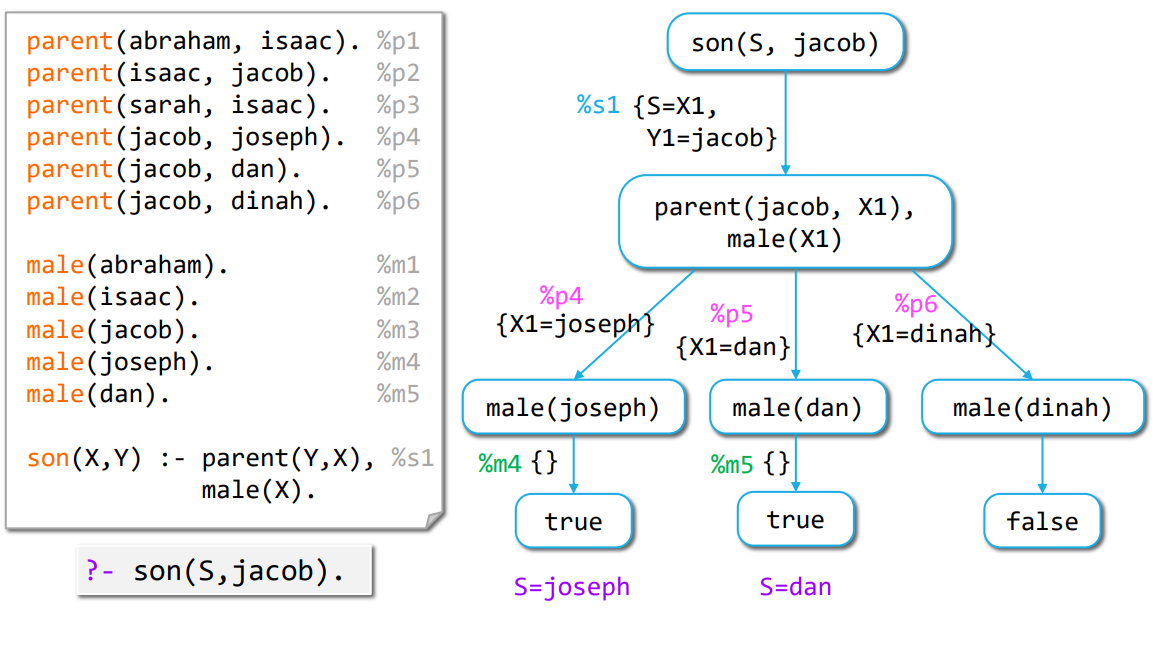
\includegraphics[width=\linewidth]{figures/proof-tree.png}
    \caption[An example of proof tree generated by the SLD resolution principle]{An example of proof tree generated by the SLD resolution principle while attempting to prove the goal $son(S, \functor{jacob})$ against the depicted knowledge base. }
    \label{fig:proof-tree}
\end{figure}

\Cref{fig:proof-tree} exemplifies the proof tree generated by the recursive application of SLD inference rule to the goal $son(S, \functor{jacob})$.
%
The resolution attempts to prove the goal against a knowledge base describing Abraham's family tree, represented in the same image.
%
Each node in the tree represents a rewritten form of the original goal, whereas each arc subtends the selection of a rule from the knowledge base and a literal from the source node: the label of each edge describes their MGU.

Of course, at each step of the SLD resolution, several choices may be taken.
%
For instance, several literals may be selected, and each literal may unify with potentially many rules in the knowledge base.
%
The theoretical formulation of the SLD principle addresses such choices via \emph{non-determinism}.
%
However, whenever an actual computational agent needs to perform automated reasoning, it must leverage upon some smart strategy to explore the proof tree sequentially, and in useful time.

\paragraph{Colmerauer's Prolog}

Prolog \cite{ColmerauerR93} is the most successful expression of the LP paradigm.
%
It is at the same time a particular way of expressing logic resolution, and a very powerful technology to perform automated reasoning in practice.
%
Here we focus on the theoretical aspects of Prolog, whereas technological aspects are treated later in this thesis.

Prolog is essentially a particular way to make the exploration of the proof tree subtended by the SLD resolution principle \emph{sequential}.
%
In other words, Prolog makes the SLD resolution a sequential algorithm.
%
More precisely, Prolog assumes goals to be \emph{ordered} disjunctions of literals (left to right), and knowledge bases to be \emph{ordered} sets of definite clauses (top to bottom).
%
Under such assumption, it adopts the following strategy while dealing with the non-determinism of SLD resolution:
%
\begin{itemize}
    \item literals in the current goal are reduced from left to right,
    \item rules are selected from top to bottom.
\end{itemize}
%
This strategy subtends a \emph{depth-first} exploration of the proof tree.

Another relevant modelling choice in Prolog concerns the syntax for predicates and terms.
%
In fact, Prolog represents predicates and structured terms in the same way, collapsing their syntaxes and making the two notions interchangeable.
%
This simplifies the definition of meta-predicates -- i.e. predicates accepting other predicates as arguments --, as terms can be used to represent predicates.
%
Meta-predicates, in turn, make Prolog's semantics very flexible, as disjunctions, implications, negations, and many other features of FOL which are not supported by Horn clauses can be re-introduced in Prolog in this way.

\paragraph{Clark's Negation as Failure}

NaF \cite{Clark77} is the last relevant extension of SLD we discuss in this section.
%
It essentially aims at supporting negation in Horn clauses.
%
SLD resolution extended with NaF is often concisely referred to as SLDNF.

SLDNF supports negation by defining the meta-predicate $not(g)$ which is proven true if and only if the argument goal $g$ is proven unsatisfiable.
%
So, in procedural terms, the goal $not(g)$ can be read as ``attempt to prove $g$, and, if no solution exists, then $not(g)$ is true, false otherwise''.

Notably, NaF subtends a \emph{closed} world assumption, where everything that is not know -- nor deducible from what is known -- is false.

\section{Sub-symbolic Reasoning}
%
\mypapers[section]{xaisurvey-ia14}

Within the sub-symbolic realm, the term `inference' is often abused.
%
There, `inference' refers to the application phase of any data-driven solution which has been previously trained on data.
%
Therefore, inference in simply a phase in the life-cycle of a data-driven model, as opposed to training.

In the inference phase of any sub-symbolic system, novel information is actually drawn, and that information strongly depends on what the systems has learned from data (prior knowledge) during training.
%
For instance, classifiers enable the labelling of arbitrarily complex unknown data according to some predefined set of labels.
%
Similarly, regressors enable predictions on unknown data, out of prior experience.
%
So, in a broad sense, sub-symbolic systems support the inference of novel, useful information.
%
By definition, however, no symbolic manipulation of data occurs in sub-symbolic systems, regardless of whether training or inference are considered.
%
Hence, it is cumbersome speaking of reasoning.

Nevertheless, a number of recent proposals are pushing relevant aspects of logic inference into the sub-symbolic realm.
%
As a result, methods for building \emph{hybrid} systems -- i.e. systems mixing symbolic and sub-symbolic means to represent, learn, or infer -- are flourishing.

Generally speaking, hybridisation may occur in two ways, namely by \emph{model integration} or by \emph{symbolic knowledge embedding}.
%
In the former case, symbolic information is used to \emph{structure} or \emph{constrain} the behaviour of a sub-symbolic system---in most cases, a neural network, because of its malleability.
%
In the latter case, symbolic information is \emph{embedded} into a sub-symbolic representation to enable its sub-symbolic processing.

\subsection{Model Integration}\label{ssec:model-integration}

In this category we review the main attempts to \emph{integrate} symbolic models (such as the logic ones) with sub-symbolic ones (such as statistical and numerical).
%
The main research lines here are those related to the neural-symbolic computing \cite{Hammer2007-neuralsymbolic}  -- the study of logics and connectionism as well as statistical approaches working on the integration of computational learning and symbolic reasoning -- and relational learning \cite{deRaedt2008-logicalRL}---focused on learning expressive logic / relational representations.

Approaches in this category integrate logic and symbolic knowledge with sub-symbolic predictors such as (deep) neural networks.
%
Integration exploits logic rules expressed via FOL -- or some subset of it -- which are used to either constrain or structure the behaviour of one or more predictors.

On the one hand, constraining is commonly performed by extending the loss function used by most numeric learning algorithms -- there including the back-propagation algorithm used for neural networks -- with an additive, regularisation term constructed from the logic constraints.
%
The numeric predictor is then trained ``as usual'', via optimisation---i.e. minimising some loss function.
%
However, thanks to a \emph{regularisation} term attained by encoding the logic rules accordingly, the training process is more likely to select a set of parameters for the numeric predictor, which are consistent with those logic rules.
%
Generally speaking, the key advantage of these approaches lies in the blended integration of different models, where the logic one -- where expressing crisp information is trivial -- can be used to inject prior knowledge or common-sense into the sub-symbolic one, even in lack of data.

On the other hand, structuring is commonly performed by building the sub-symbolic predictors in such a way that their internal structure mirrors the provided symbolic knowledge.
%
For this reason, malleable models such as neural networks are often preferred to serve this purpose.
%
There, the internal topology of neurons, as well as their activation functions, are structured in such a way to mimic some relevant property of given logic rules---such as their interpretation.
%
Computation is then shifted into the sub-symbolic realm, since the so-constructed predictors act ordinarily.
%
Generally speaking, the key advantage of these approaches sub-symbolic emulation of symbolic facilities, thus allowing efficiency of reasoning in particular cases -- at the price of constraining it scope of application --, and robustness w.r.t. missing or contradictory data.

\paragraph{Logic as constraints}

Paradigmatic works in this category are for instance: DNN with Logic Rules \cite{hu2016}, Logic Tensor Networks (LTN) \cite{serafini2016,Serafini2017}, Semantic Loss Function (SLF) \cite{xu2018}, and Lyrics \cite{MarraGDG2019}.

DNN with Logic Rules (no concise name is given) \cite{hu2016}, proposes a method for constraining a (deep) neural network behaviour via FOL rules.
%
The proposed framework enables neural networks to be simultaneously trained on labelled data or logic rules, via an iterative distillation procedure aimed at transferring the symbolic knowledge encoded in the logic rules into the network parameters.
%
To do so, the authors propose the exploitation of two networks: a \emph{teacher} and a \emph{student} one.
%
The teacher network is rule-regularised via an \emph{ad-hoc} term added to the loss function, meaning that it is trained by keeping into account the user-provided logic rules.
%
In particular, logic constraints are encoded into the loss function via soft logic \cite{BachBHG17}.
%
Conversely, the student network is trained to balance between emulating the teacher network output and predicting the expected outcomes of the dataset.

LTN \cite{serafini2016,Serafini2017} integrate learning based on tensor networks \cite{socher2013} with reasoning based first-order many-valued logic \cite{bergmann2008}.
%
They enable a range of knowledge-based tasks using rich knowledge representation in FOL to be combined with efficient data-driven machine learning based on the manipulation of real-valued vectors.
%
% Given data available in the form of real-valued vectors, logic soft and hard constraints, and relations that apply to certain subsets of the vectors can be specified in a compact way using FOL.
% %
% Reasoning about the constraints can help improve learning, and, viceversa, learning from new data can revise the constraints thus affecting the reasoning task.
%
Notably, integration is defined upon the Real Logic \cite{Serafini2017}.
%
FOL formul\ae{} are used to build a loss function that aims at training a network capable of approximating the truth value (in the $[0,1]$ interval) of the formul\ae{} given as input.
%
This is done by searching for the best possible representation for symbolic constructs in a vector space (grounding of atoms, functions, predicates), so that the satisfiability of the network is as close as possible to 1 on the test dataset.
%
The resulting network is able to learning from the rightly-labelled real examples, but keeps the logic imprint given in the training phase.

SLF \cite{xu2018} is another attempt of bridging neural networks and symbolic constraints via loss-function manipulation, similarly to LTN.
%
In the intentions of its authors, it aims to
%
\begin{itemize}
    \item improve the predictive performance of neural networks -- by allowing the training process to take background knowledge into account --, and
    \item support semi-supervised learning.
\end{itemize}
%
To do so, SLF constrains the training process of a neural network via some \emph{propositional} logic formul\ae{} which are then encoded as part the loss function exploited by the training algorithm.
%
Such formul\ae{} consist of boolean variables representing input and output neurons of the networks to be constrained, possibly combined via classical logic connectors.

Finally, Lyrics \cite{MarraGDG2019} is an extension of LTN, improving the way symbolic knowledge is declaratively enforced while training the sub-symbolic part of an intelligent system.
%
According to the authors, the major applications of Lyrics are related to predictive model verification, semi-supervised learning with background knowledge, collective classification \cite{SenNBGGE08}, and text chunking.
%
Similarly to LTN, Lyrics can combine one or more neural networks into a single computational graph.
%
Each neural network is mapped onto a logic predicate, when necessary, while (possibly global) constrains over the outcomes of the networks are mapped into logic formul\ae{}.
%
The resulting computational graph is then optimised against the available data via state-of-the-art gradient-descent technologies---e.g. TensorFlow.

\paragraph{Logic as structure}

Paradigmatic works in this category are for instance: Knowledge-Based Artificial Neural Networks (KBANN) \cite{Towell1990}, CILP++ \cite{Franca2014}, Neural Theorem Prover (NTP) \cite{rocktaschel2017}, Differentiable Inductive Logic Programming ($\partial$ILP) \cite{EvansG18}, DeepProbLog \cite{Manhaeve2018}, and Lifted Relational Neural Networks (LRNN) \cite{SourekAZSK18}.

KBANN \cite{Towell1990} is one of the earliest attempts of exploiting symbolic AI to govern the structure and the behaviour of neural networks.
%
It is capable of devising the structure of a neural network from a symbolic knowledge base containing the user-defined, symbolic background knowledge.
%
More precisely, KBANN assumes a stratified, Prolog-like, logic theory is available, encoding the background knowledge.
%
Under this assumption, the KBANN algorithm aims at creating a neural network semantically reflecting the symbolic knowledge from which it was created.
%
This step essentially sets the network structure and weights in order to reflect the rules contained into the logic theory.
%
The resulting neural network can then be trained over data via back-propagation, in order to refine or generalise its functioning over (possibly novel) data.
%
% According to the authors, the KBANN algorithm has proven to be useful in the area of molecular biology.
%
% In particular, neural networks attained via KBANN has been used to detect promoters in strings of nucleotides, with superior performance w.r.t. randomly initialised neural networks or other sorts of numeric predictors.

CILP++ \cite{Franca2014} is a model aimed at performing inductive logic programming (ILP) via bottom clause propositionalisation and neural networks.
%
CILP++ leverages on
%
\begin{inlinelist}
    \item neural networks to make ILP faster, and on
    \item propositionalisation to make the construction of neural networks out of arbitrary logic theories possible.
\end{inlinelist}
%
More precisely, propositionalisation \cite{Lachiche2010} is a preliminary step, which is necessary to convert the example clauses into real vectors and the background knowledge into a multi-layered neural network to be fed with those vectors.
%
Of course, the structure of this network reflects the rules contained in the background knowledge, and the input layer contains a neuron for each possible atom used in the background knowledge.

NTP \cite{rocktaschel2017} are neural networks acting as logic reasoners (a.k.a. theorem provers).
%
They are built by taking inspiration from backward-chaining-based reasoning algorithms, as in Prolog.
%
In particular, the neural network is recursively constructed to encapsulate the knowledge encoded in some logic theory, and trained to correctly answer to all possible queries on such theory.
%
Of course, the structure of the resulting network reflects the structure of the clauses contained into the source logic theory.
%
However, differently from the other techniques presented in this sub-category, both theories and queries supported by NTP can contain logic variables, as NTP is able to calculate, at the neural network level -- i.e., in the sub-symbolic model --, the logic unification.
%
In other words, NTP perform symbolic reasoning on top of sub-symbolic and distributed representations of knowledge.

$\partial$ILP \cite{EvansG18} is another means for ILP  leveraging on neural networks.
%
It works by mimicking logic deduction on definite clauses via a neural network, similarly to NTP.
%
However, differently from NTP, $\partial$ILP perform deduction using forward chaining, instead of backward chaining.
%
Briefly speaking, the authors re-interpret ILP as a binary-classification problem.
%
As for other similar approaches discussed in this category, a neural network is constructed in such a way that its structure reflects a grounded version of the background knowledge.
%
The resulting network is then trained to minimise the cross-entropy with respect to positive and negative examples.

DeepProbLog \cite{Manhaeve2018} is another attempt of blending neural networks with logic programming, and in particular \emph{probabilistic} logic programming (PLP).
%
It is an extension of ProbLog exploiting neural networks for
%
\begin{inlinelist}
    \item computing the probabilities of facts, and
    \item letting neural classifiers be used as logic predicates---defined as ``neural predicates'' by the authors.
\end{inlinelist}
%
In particular, each DeepProbLog program is translated into a tensorial computational graph -- possibly including one or more neural classifiers as sub-graphs -- to be optimised via gradient descend.
%
The structure of the computational graph reflects the structure of the rules contained into the DeepProbLog program.
%
The optimisation step is aimed at simultaneously setting all the possible parameters regulating the behaviour of the computational graph, including the probabilities of facts and the internal weights of neural predicates.
%
The resulting sub-symbolic system is then exploited to draw probabilistic inferences.
%
In other words, hybrid systems based on DeepProbLog fruitfully combine probabilistic reasoning and sub-symbolic classification in a single, unified, coherent framework.

Finally, LRNN \cite{SourekAZSK18} aim at performing relational learning from data via neural networks.
%
Similarly to DeepProbLog, LRNN exploit sets of weighted first-order formul\ae{} as structural templates for building a neural network to be trained over the available data.
%
The resulting network is exploited to infer latent rules buried in data and to estimate the weights of the existing clauses.

\subsection{Symbolic Knowledge Embedding}

In this category we review the main attempts to \emph{embed} symbolic (and, in particular, logic) knowledge into arrays of numbers, to make them amenable of sub-symbolic processing.

Most techniques developed so far are tailored on \emph{description logics}, that are particular sub-sets of FOL generally aimed at describing categories of entities and their possible relations, along with instances of both.
%
The key idea is to translate components of an ontology (a.k.a.\ knowledge graph, or simply KG) into continuous vector spaces, to allow neural networks to accept such a type of structured information as input and take advantage of its background knowledge to perform ordinary machine learning tasks.

Most of the currently-available techniques perform the embedding task only on the basis of observed facts.
%
Given a KG, knowledge graph injection techniques first represent entities and relations in a continuous vector space, and then measure facts plausibility exploiting some scoring function.
%
Entity and relation embeddings can be obtained by maximising the total plausibility of observed facts.

During this whole procedure, the learned embeddings are only required to be compatible within each individual fact, and hence might not be predictive enough for downstream tasks \cite{wang2015,wei2015}.
%
As a result, more and more researchers have started to add other types of information, including logic rules \cite{wang2015,rocktaschel2015,guo2016}, in order to learn more predictive embeddings.

The noteworthy approaches that we deem significant for the purpose of this survey -- as they combine symbolic and sub-symbolic models -- are:
%
\begin{itemize}
	\item \textsc{Rescal} + \textsc{Trescal} (2015) \cite{wang2015}
	\item \textsc{Ins} (2015) \cite{wei2015}
	\item Low-rank Logic Embeddings, LLE (2015) \cite{rocktaschel2015}
	\item \textsc{Kale} (2016) \cite{guo2016}
	\item \textsc{Oscar} (2019) \cite{goodwin2019}
\end{itemize}
%
In particular, \cite{wang2015,wei2015} exploit rules to refine embedding models aimed at KG completion.
%
KG completion is formulated as an integer linear programming problem, where the objective function is generated from embedding models and constraints are generated from rules.
%
Facts inferred in this way are the most preferred by the embedding models and comply with all the rules.
%
By incorporating rules, these approaches can greatly reduce the solution space and significantly improve the inference accuracy of embedding models.
%
\textsc{Trescal} \cite{wang2015} is an extension of \textsc{Rescal}, requiring the arguments of a relation to be entities of certain specified types.

Along this line, other works -- e.g., \cite{rocktaschel2015,guo2016} -- propose approaches that embed KG facts and logic rules simultaneously in a unified framework.
%
In particular, in \textsc{Ins}, formul\ae{} are injected into the embeddings of relations and entity-pairs, i.e., the embeddings are estimated such that predictions based on them conform to given logic formul\ae.
%
\textsc{Kale}, on the other side, represents rules as complex formul\ae{} modelled by t-norm fuzzy logics.
%
Embedding then amounts to minimising a global loss over both atomic and complex formulae.
%
Thus embeddings are learnt as compatible with rules.

In \cite{goodwin2019} the authors propose a method, \textsc{Oscar}, for injecting task-agnostic knowledge from a KG into a neural network during the training.
%
\textsc{Oscar} is a pre-training regularisation technique capable of injecting world knowledge and ontological relationships into a deep neural network: the expert knowledge is exploited as a regulariser for the network.

It is worth noting that in all these approaches rules are modelled separately from embedding models, serving as post-processing steps: this is why we classify these work as combination and not integration.
%
Furthermore, all these works share a common drawback, in that they have to instantiate universally-quantified rules into ground rules before learning their models.
%
This is called grounding procedure, and can be time- and space-inefficient---especially when dealing with big data scenarios or in case of rules complexity.

\subsection{Hybrid Systems: Final Remarks}

Hybrid systems are still in their infancy.
%
Hybridisation usually comes at the cost of a reduced expressiveness of the logic formalism adopted.
%
Empirically, we observe that full fledged FOL is too complex to handle for sub-symbolic systems, which are therefore forced to take countermeasures into account.
%
Once again, issues concern KR.
%
In particular, \emph{intensional} logic representations as well as the flexibility of logic -- which is open to the addition of novel symbols --, are what makes hybridisation difficult.

Countermeasures generally involve using a sub-sets of FOL -- thus renouncing to the full expressiveness of FOL --, and enforcing knowledge to be extensively represented.

In the former case, constraints are imposed at the KR level.
%
These may involve
%
\begin{inlinelist}
    \item forbidding structured terms,
    \item limiting the shape of predicates or clauses,
    \item focussing on simpler logics such as Horn logic, description logics, or predicate logic,
    \item or a combination of these constraints.
\end{inlinelist}\
%
In all such cases, the scope of the hybrid system is reduced, w.r.t. a full-fledged symbolic system.
%
Consider for instance the case of Horn logic with no structured terms.
%
This would imply, for instance, that lists could not be used in the symbolic part of the system---hence greatly reducing the practical reach of hybrid systems.

In the latter case, \emph{grounding} of the knowledge base is usually assumed as a preliminary step before any sub-symbolic processing.
%
In the general case, grounding a non-ground knowledge base involves enumerating all the possible variable assignments of for all variables of all formul\ae{} therein contained.
%
Variable assignments may in turn be infinite, depending on how may items the underlying Herbrand universe contains.
%
Of course, grounding is only possible in practice when the amount of items in the Herbrand universe -- and therefore the amount of admissible variable assignments --, is \emph{finite}.
%
Notably, by admitting structured terms for KR, the Herbrand universe will certainly be infinite (cf. \cref{par:herbrand})---hence why leveraging on grounding usually subtends forbidding (at least) structured terms from the KR formalism.

\chapter{Explaining AI via Symbolic Knowledge}
\label{chap:explaining}

% Despite the open philosophical issues, i
It is undeniable that AI and ML are nowadays becoming more and more intertwined with a growing number of aspects of people's every day life \cite{helbing2019, elliott2019}.
%
In fact, more and more decisions are delegated by humans to software agents whose intelligent behaviour is not the result of some skilled developer endowing them with some clever code, but rather the consequence the agents' capability of learning, planning, or inferring what to do from data.

In spite of the large adoption, intelligent machines whose behaviour is the result of automatic synthesis / learning procedures are difficult to trust for most people---in particular when they are not expert in the field.
%
This is especially true for agents leveraging on machine or deep learning based techniques, often producing models whose internal behaviour is opaque and hard to explain for their developers too.

There, agents often tend to accumulate their knowledge into \emph{black-box} predictive models which are trained through ML or DL.
%
As we further discuss in this chapter, ``black boxes'' are models where knowledge is \emph{sub-symbolically} represented -- such as NN, support vector machines (SVM), or random forests --, and it is therefore difficult, for humans, to understand what they actually know, or what led them to a particular decision.

Such difficulty in understanding black-boxes content and functioning is what prevents people from fully trusting -- and thus accepting -- them.
%
In several contexts, such as the medical or financial ones, it is not sufficient for intelligent agents to output bare decisions, since, for instance, ethical and legal issues may arise.
%
An \emph{explanation} for each decision is therefore often desirable, preferable, or even required.
%
Furthermore, it may happen for instance that black-boxes \emph{silently} learn something wrong (e.g., Google image recognition software that classified black people as gorillas \cite{fourcade2017, crawford2016artificial}), or something right, but in a biased way (like  the ``background bias'' problem, causing for instance husky images to be recognised only because of their snowy background \cite{RibeiroSG16}).

% To tackle such trust issues, the \emph{eXplainable Artificial Intelligence} (XAI) research field has recently emerged, and a comprehensive research road map has been proposed by DARPA \cite{darpa2016-xai}, targeting the themes of explainability and interpretability in AI -- and in particular ML -- as a challenge of paramount importance in a world where AI is becoming more and more pervasively adopted.
% %
% There, DARPA reviews the main approaches to make AI either more interpretable or \emph{a posteriori} explainable, it categorises the many currently available techniques aimed at building meaningful interpretations or explanations for black-box models, it summarises the open problems and challenges, and it provides a reference framework for the researchers interested in the field.

% Broadly speaking, research efforts in the field of XAI are focused on achieving key properties in AI, such as \emph{interpretability}, \emph{transparency}, \emph{explainability}, \emph{accountability}, and \emph{trustworthiness}.
% %
% Unfortunately, such goals are still far from being reached.
% %
% For instance, as pointed out in \cite{Lipton18}, the aforementioned properties are still lacking a formal and agreed-upon definition.
% %
% Some authors \cite{Rudin2019} propose to strengthen the adoption of most \emph{interpretable} (i.e. algorithmically transparent) predictive models -- such as generalised linear models or decision trees --, while others seek new ways to produce \emph{post-hoc} explanations capable of tackling even most opaque predictors, such as NN.
% %
% However, as demonstrated by the comprehensive survey produced by Guidotti et al. \cite{GuidottiMRTGP19}, most works only target classification problems, and they rarely take wider properties -- such as accountability and trustworthiness -- into account.

% \sidenote{Spostare il capoverso sotto in un posto più opportuno}
% Several works, among the various springs of AI, proposed to extract symbolic knowledge from sub-symbolic models.
% %
% As witnessed by a number of surveys \cite{GuidottiMRTGP19, GarcezBRFHIKLMS15, AndrewsDT95, GarcezBG01} and works on the topic \cite{BolognaH18, BolognaH16, FrosstH17, JohanssonN09, KrishnanSB1999, HruschkaE2006, ZhouZYS1983, CravenS95, AugastaK12, SatoT2002, KahramanliA09a} -- some of which are from the 80s or the 90s -- the potential of symbolic knowledge \emph{extraction} is well understood, despite not being subject to hype.
% %
% Unfortunately, a comprehensive and general framework tackling such problem in a general way is still missing.

% \note{Armonizzare quanto segue con ciò che precede}

% Since the adoption of interpretable predictors usually comes at cost of a lower potential in terms of predictive performance, \emph{explanations} are the newly preferred way for providing understandable predictions without necessarily sacrificing accuracy.
% %
% The idea, and the main goal of XAI is to create intelligible and understandable explanations for uninterpretable predictors \emph{without} replacing or modifying them.
% %
% Thus explanations are built through a number of heterogeneous techniques, broadly referred to as \emph{explanators} \cite{GuidottiMRTGP19}---just to cite some, \emph{decision rules} \cite{AugastaK12}, \emph{feature importance} \cite{tolomei2017interpretable}, saliency masks \cite{FongV17}, sensitivity analysis \cite{SundararajanTY17}, etc.

% The state of the art for explainability currently recognises two main sorts of explanators, namely, either local or global.
% %
% While \emph{local} explanators attempt to provide an explanation for each particular prediction of a given predictor $p$, the \emph{global} ones attempt to provide an explanation for the predictor $p$ as a whole.
% %
% In other words, local explanators provide an answer to the question ``why does $p$ predict $\mathbf{y}$ for the input $\mathbf{x}$?'' -- such as the LIME technique presented in \cite{RibeiroSG16} --, whereas global explanators provide an answer to the question ``how does $p$ build its predictions?''---such as decision rules.

% In spite of the many approaches proposed to explain black boxes, some important scientific questions still remain unanswered.
% %
% One of the most important open problems is that, until now, there is no agreement on what an explanation is.
% %
% Indeed, some approaches adopt as explanation a set of rules, others a decision tree, others rely on visualisation techniques \cite{GuidottiMRTGP19}.
% %
% Moreover, recent works highlight the importance for an explanation to guarantee some properties, e.g., soundness, completeness, and compactness \cite{GuidottiMRTGP19}.

% \note{Probabilmente si può tagliare da qui in poi}

% This is why our proposal aims at integrating sub-symbolic approaches with symbolic ones.
% %
% To this end, DT can be exploited as an effective bridge between the symbolic and sub-symbolic realms.
% %
% In fact, DT can be easily \emph{(i)} built from an existing sub-symbolic predictor, and \emph{(ii)} translated into symbolic knowledge -- as it is shown in the reminder of this paper -- thanks to their rule-based nature.

% Decision trees are an interpretable family of predictors that have been proposed as a \emph{global} means for explaining other, less interpretable, sorts of black-box predictors \cite{TrattnerPR2019,BastaniKB17}---such as neural networks \cite{CravenS95}.
% %
% The main idea behind such an approach is to build a DT approximating the behaviour of a given predictor, possibly, by only considering its inputs and its outputs.
% %
% Such approximation essentially trades off predictive performance with interpretability.
% %
% In fact, the structure of such a DT would then be used to provide useful insights concerning the original predictor inner functioning.

% Describing the particular means for extracting DT from black-boxes is outside the scope of this paper.
% %
% Given the vast literature on the topic -- e.g., consider reading \cite{GuidottiMRTGP19,AndrewsDT95} for an overview or \cite{CravenS95,JohanssonN09,FrosstH17} for a practical examples -- we simply assume an extracted DT is available and it has an high \emph{fidelity}---meaning that the loss in terms of predictive performance is low, w.r.t. the original black-box.
% %
% In fact, whereas there exist several works focussing on how to synthesise DT out of black-box predictors, no attention is paid to merging them with symbolic approaches, which can play a key role in enhancing the interpretability and explainability of the system.
% %
% In this paper we focus on such a matter.

% We believe that a logical representation of DT may be interesting and enabling for further research directions.
% %
% For instance, as far as explainability is concerned, we show how logic-translated DT can be used to both navigate the knowledge stored within the corresponding predictors -- thus acting as \emph{global} explanators --, and produce \emph{narrative} explanations for their predictions---thus acting as \emph{local} explanators.
% %
% Note that the restriction on the DT representation makes it easy to map DT onto logical clauses, since DT are finite and with a limited expressivity (if / else conditions).

Accordingly, in the reminder of this chapter we discuss the meaning and the role of explanations in modern AI, we review the recent literature on this topic, and we present the possible means to construct \emph{symbolic} explanations for sub-symbolic predictors.

%===============================================================================
\section{eXplainable Artificial Intelligence}\label{sec:xai-background}
%===============================================================================

\mypapers[section]{agentbasedxai-aamas2020,agentbasedxai-extraamas2020}

Most intelligent systems (IS) today leverage on \emph{numerical} predictive models which are trained from data through ML.
%
The reason for such a wide adoption is easy to understand.
%
We live in an era where the availability of data is unprecedented, and ML algorithms make it possible to semi-automatically detect useful statistical information hidden into such data.
%
Information, in turn, supports decision-making, monitoring, planning, and forecasting in virtually any human activity where data is available.

However, ML is not the silver bullet.
%
Despite the increased predictive power, ML comes with some well-known drawbacks which make it perform poorly in some use cases.
%
One blatant example is algorithmic \emph{opacity}---that is, essentially, the difficulty of human mind in \emph{understanding} how ML-based IS function or compute their outputs.
%
Such difficulty is a serious issue in all those contexts where human beings are liable for their decision or must provide some sort of \emph{explanation} for it---even if the decision has been supported by some IS.
%
For instance, think about a doctor willing to motivate a serious, computer-aided diagnosis, or, a bank employee in need of explaining to a customer why his/her profile is inadequate for a loan.
%
In all contexts, ML is at the same time an enabling -- as it aids the decision process by automating it -- and a limiting factor---as opacity prevents human awareness of \emph{how} the decision process works.

Opacity is why ML predictors are also referred to as \emph{black boxes} into the literature.
%
The ``black box'' expression refers to models where knowledge is not explicitly represented \cite{Lipton18}.
%
The lack of some explicit, symbolic representation of knowledge is what makes it hard for humans to \emph{understand} the functioning of black boxes, and why they led to suggest or undertake a given decision.
%
Obviously, troubles in understanding black-box content and functioning prevents people from fully trusting -- therefore accepting -- them.
%
To make the picture even more complex, current regulations such as the GDPR \cite{gdpr-voigt2017} are starting to recognise the citizens' \emph{right to explanation} \cite{explanation-aimag38}---which implicitly requires IS to eventually become \emph{understandable}.
%
In fact, understanding IS is essential to guarantee algorithmic fairness, to identify potential bias/problems in the training data, and to ensure that IS perform as designed and expected.

%%%%
\begin{figure}
    \centering
    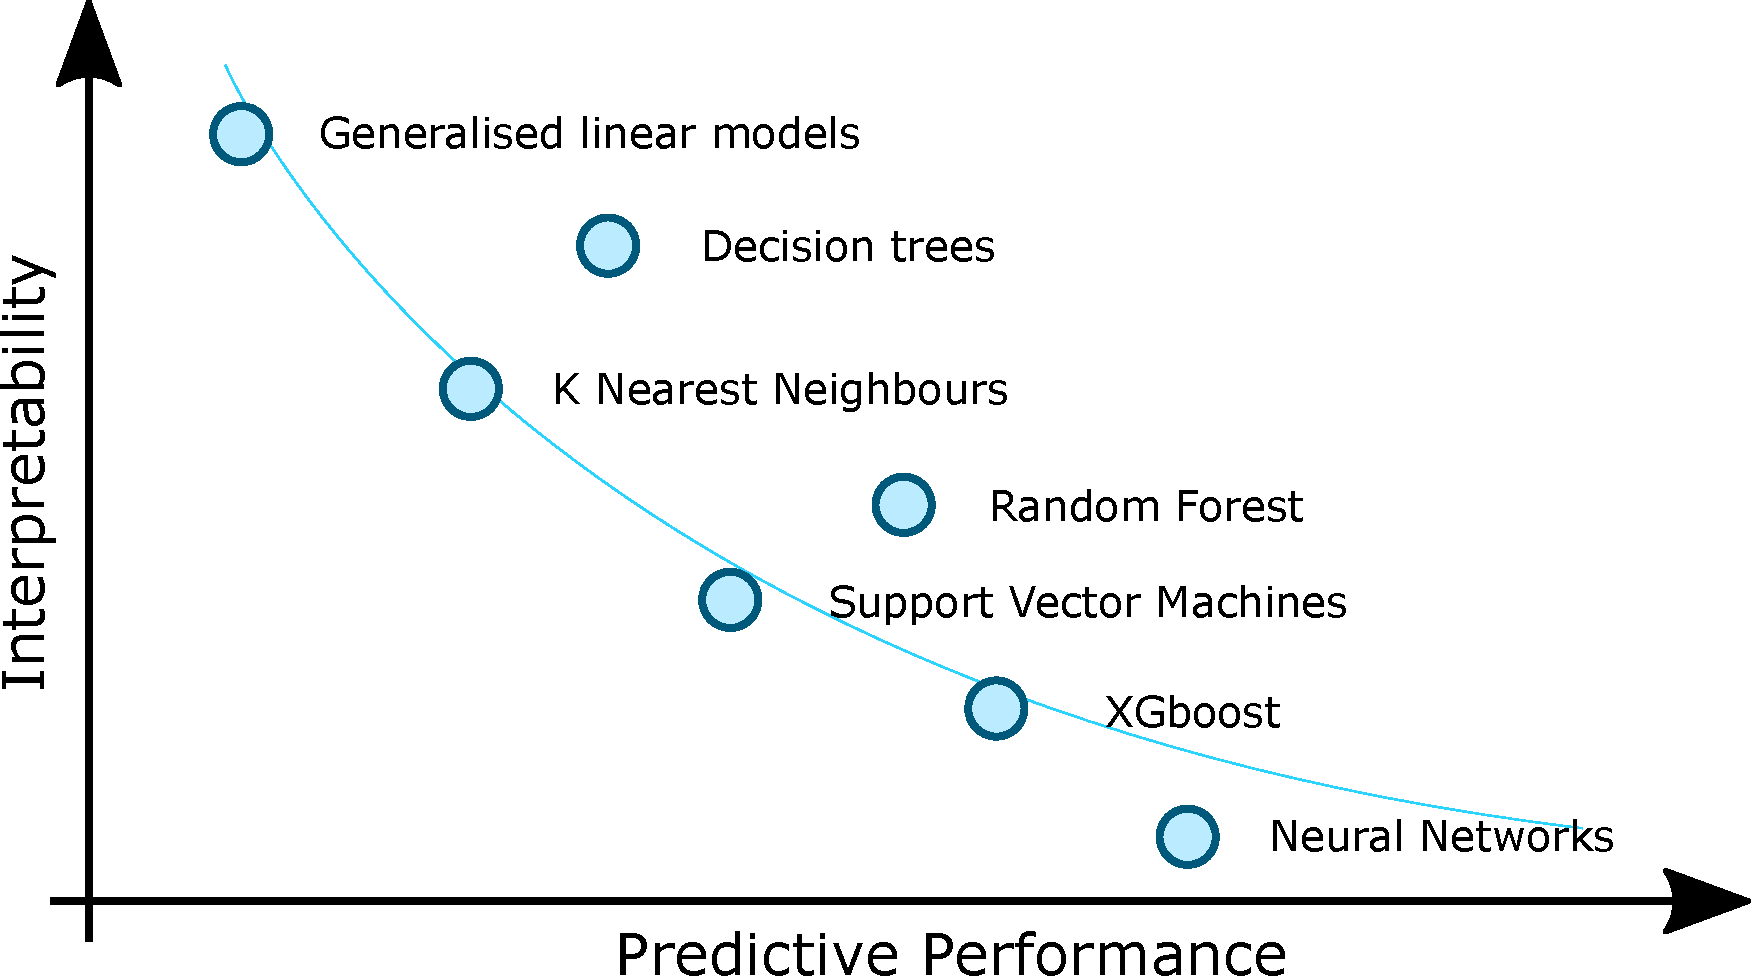
\includegraphics[width=.8\linewidth]{figures/interpretability-performance-tradeoff}
    \caption[Interpretability/performance trade-off]{Interpretability/performance trade-off for some common sorts of black-box predictors}
    \label{fig:tradeoff}
\end{figure}
%%%%

Unfortunately, the notion of understandability is neither standardised nor systematically assessed, yet.
%
At the same time, there is no consensus on what exactly providing an \emph{explanation} should mean when decisions are supported by a black box.
%
However, several authors agree that not all black boxes are equally \emph{interpretable}---meaning that some black boxes are easier to understand than others for our mind.
%
For example, \cref{fig:tradeoff} is a common way to illustrate the differences in black-box interpretability.

Even though informal -- as pointed on in \cite{Rudin2019}, given the lack of way to measure ``interpretability'' -- \cref{fig:tradeoff} effectively express why more research is need on understandability.
%
In fact, the image essentially states how the better performing black boxes are also the less interpretable ones.
%
This is a problem in practice since only rarely predictive performances can be sacrificed in favour of a higher degree of interpretability.

To tackle such issues, the \emph{eXplainable AI} (XAI henceforth) research field has recently emerged.
%
Among the many authors and organisations involved in the topic, DARPA has proposed a comprehensive research road map \cite{darpa2016-xai} which reviews the main approaches to make black boxes more understandable.
%
There, DARPA categorises the many currently available techniques aimed at building meaningful interpretations or explanations for black-box models, it summarises the open problems and challenges, and it provides a successful reference framework for the researchers interested in the field.
%
Unfortunately, in spite of the great effort in defining terms, objects, and methods for the research line, a clear definition of fundamental notions such as \emph{interpretation} and \emph{explanation} is still missing.

%-------------------------------------------------------------------------------
\subsection{Related works}\label{ssec:related}
%-------------------------------------------------------------------------------

Notions such as explanation, interpretation, transparency, etc., are mentioned, introduced, or informally defined in several works.
%
However, a coherent framework has not emerged yet.

In this subsection we recall some main contributions from the literature where the concepts of explanation and interpretation -- or any variant of theirs -- are discussed.
%
Our goal here is to highlight the current lack of consensus on the meaning of such terms, for which we propose a possible, unambiguous alternative in the next sections.

Similarly to what we do here, Lipton \cite{Lipton18} starts his discussion by recognising how most definition of ML interpretability are often inconsistent and underspecified.
%
In his clarification effort, Lipton essentially maps interpretability on the notion of \emph{transparency}, and explanation on the notion of \emph{post-hoc} interpretation.
%
Then, he enumerates and describes the several possible variants of transparency, that are
%
\begin{inlinelist}
    \item simulatability -- i.e., the \emph{practical} possibility, for a human being, to ``contemplate the entire model at once'' and simulate its functioning on some data  -- which characterises, for instance, generalised linear models;

    \item decomposability -- i.e., the possibility, for the model to be decomposed in elementary parts whose functioning is intuitively understandable for humans and helpful in understanding the whole model -- which characterises, for instance, decision trees; and

    \item algorithmic transparency -- i.e., the possibility, for a human being, to intuitively understand how a given learning algorithm, or the predictors it produces, operate -- which characterises, for instance, k-nearest-neighbours techniques.
\end{inlinelist}
%
Similarly, \emph{post-hoc} interpretability is defined as an approach where some information is extracted from a black box in order to ease its understanding.
%
Such information have not necessarily to expose the internal functioning of the black box.
%
As stated in the paper: ``examples of post-hoc interpretations include the verbal explanations produced by people or the saliency maps used to analyse deep neural networks''.

Conversely, Besold et al. \cite{BesoldU2018} discuss the notion of explanation at a fundamental level.
%
There, the authors provide a nice philosophical overview on such topic, concluding that ``explanation is an epistemological activity and explanations are an epistemological accomplishment---they satisfy a sort of epistemic longing, a desire to know something more than we currently know. Not only do they satisfy this desire to know, they also provide the explanation-seeker a direction of action that they did not previously have''.
%
Then they discuss the topic of explanation in AI from an historical perspective.
%
In particular, when focussing on ML, they introduce the following classification of IS systems:
%
\begin{inlinelist}
    \item opaque systems -- i.e., black boxes acting as oracles where the logic behind predictions is not observable or understandable --,

    \item interpretable systems -- i.e., white boxes whose functioning is understandable to humans, also thanks to expertise, resources, or tools --, and

    \item comprehensible systems---i.e., ``systems which emit \emph{symbols} along with their outputs, allowing the user to relate properties of the input to the output''.
\end{inlinelist}
%
According to this classification, while interpretable systems can be inspected to be understood -- thus letting observer draw their explanations by themselves --, comprehensible systems must explicitly provide a symbolic explanation of their functioning.
%
The focus there is thus on \emph{who} produces explanations, rather than \emph{how}.

In \cite{DoshiVelezK2017}, interpretability of ML systems is defined as ``the ability to explain or to present in understandable terms to a human''.
%
Interpretations and explanations are therefore collapsed in this work, as confirmed by the authors using the two terms interchangeably.
%
The reminder of that paper focuses
\begin{inlinelist}
    \item on identifying under which circumstances interpretability is needed in ML, and
    \item how to assess the quality of some explanation.
\end{inlinelist}

The survey by Guidotti et al. \cite{GuidottiMRTGP19} is a nice entry point to explainable ML.
%
It consists of an exhaustive and recent survey overviewing the main notions, goals, problems, and (sub-)categories in this field and it encompasses a taxonomy of existing approaches for ``opening the black box''---which may vary a lot depending on the sort of data and the family of predictors at hand.
%
There, the authors define the verb to interpret as the act of ``providing some meaning of explaining and presenting in understandable terms some concepts'', borrowing such a definition from the Merriam-Webster\footnote{\url{https://www.merriam-webster.com/dictionary/interpret}} dictionary.
%
Consequently, they define interpretability as ``the ability to explain or to provide the meaning in understandable terms to a human''---a definition they again borrow from \cite{DoshiVelezK2017}.
%
So, in this case as well the notions of \emph{interpretation} and \emph{explanations} are collapsed.

In \cite{Rudin2019}, Rudin does not explicitly provide a definition for explainability or interpretability, and she refers about interpretable or explainable ML almost interchangeably.
%
However, she states some interesting properties about \emph{interpretability}, which influenced our work.
%
In particular, she acknowledges that ``interpretability is a domain-specific notion''.
%
Furthermore, she links interpretability of information with its complexity -- and, in particular, its \emph{sparsity} --, as the amount of cognitive entities the human mind can at one is very limited ($\sim 7 \pm 2$ according to \cite{numberseven-psyrev63}).
%
As far as explainability is concerned, apparently, Rudin adopts a \emph{post-hoc} perspective similar to the one in \cite{Lipton18}, as she writes ``an explanation is a separate model that is supposed to replicate most of the behaviour of a black box''.
%
In the reminder of the paper, the author argues how the path towards interpretable ML steps through a wider adoption of inherently interpretable predictors -- such as generalised linear models or decision trees -- instead of the relying on \emph{post-hoc} explanations which do not reveal what is inside black boxes---thus preventing their full understanding.

Finally, the recent article by Rosenfeld et al. \cite{RosenfeldR2019} is similar in its intents to our current work.
%
There, the authors attempt to formally define what explanation and interpretation respectively are in the case of ML-based classification.
%
% However, their work differs from ours in several ways.
%
% In particular, they define interpretation and explanation differently from what we do.
%
% In fact, a
According to the authors, ``interpretation'' is a function mapping data, data schemes, and predictors to some representation of the predictors internal logic, whereas ``explanation'' is defined as ``the human-centric objective for the user to understand'' a predictor using the aforementioned interpretation function.
%
Other notions are formally defined into the paper, such as for instance,
%
\begin{inlinelist}
    \item explicitness,
    \item fairness,
    \item faithfulness,
    \item justification, and
    \item transparency.
\end{inlinelist}
%
Such concepts are formally defined in terms of the aforementioned interpretation and explanation functions.
%
The reminder of the paper then re-interprets the field of XAI in terms of all the notions mentioned so far.

\section{Explanation vs. Interpretation}\label{sec:exp-int-basics}

This section introduces the preliminary notions, intuitions, and notations we leverage upon in \cref{ssec:framework} and subsequent sections, in order to formalise our abstract framework for agent-based explanations.
%
We start by providing an intuition for the notion of \emph{interpretation}, and, consequently, for the \emph{act} of interpreting something.
%
Accordingly, we provide an intuition for the property of ``being interpretable'' as well, stressing its comparative nature.
%
Analogously to what we did with \emph{interpretation}, we then provide intuitions for terms such as \emph{explanation} and its derivatives.

%---
\paragraph{About interpretation}
%---

Taking inspiration from the field of Logics, we define the \emph{act} of ``interpreting'' some object $X$ as the activity performed by an agent $A$ -- either human or software -- assigning a \emph{subjective} meaning to $X$.
%
Such meaning is what we call \emph{interpretation}.
%
Roughly speaking, an object $X$ is said to be  \emph{interpretable} for an agent $A$ if it is \emph{easy} for $A$ to draw an interpretation for $X$---where ``easy'' means $A$ requires a low \emph{computational} (or \emph{cognitive}) effort to understand $X$.
%
For instance, consider the case of road signs, which contain symbols instead of scripts to be easily, quickly, and intuitively interpretable.

We model such intuition through a function $I_A(X) \mapsto [0, 1]$ providing a \emph{degree of interpretability} -- or simply interpretability, for short -- for $X$, in the eyes of $A$.
%
The value $I_A(X)$ is not required to be directly observable or measurable in practice, since agents' mind may be inaccessible in most cases.
%
This is far from being an issue, since we are not actually interested in the absolute value of $I_A(X)$, for some object $X$, but rather we are interested in being able to order different objects w.r.t.\ their subjective interpretability.
%
For instance, we write $I_A(X) > I_A(Y)$, for two objects $X$ and $Y$, meaning that the former is more interpretable than the latter, according to $A$.

For example, consider the case of a neural network and a decision tree, both trained on the same examples to solve the same problem with similar predictive performances.
%
Both objects may be represented as graphs.
%
However, it is likely for a human observer to see the decision tree as more interpretable---as their nodes bring semantically meaningful, high-level information.

Summarising, we stress the subjective nature of interpretations, as agents assign them to objects according to their State of Mind (SoM) \cite{PremackW1978} and background knowledge, and they need not be formally defined any further.

%%%%
\begin{figure}
    \centering
    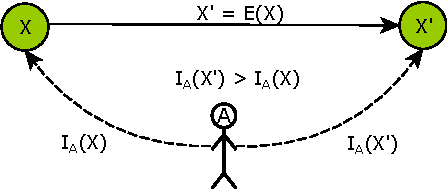
\includegraphics[width=.5\linewidth]{figures/framework.pdf}
    \caption{Explanation vs. Interpretation: a simple framework}
    \label{fig:framework}
\end{figure}
%%%%

%---
\paragraph{About explanation}
%---

We define ``explaining'' as the activity of producing a more interpretable object $X'$ out of a less interpretable one, namely $X$, performed by agent $A$.
%
More formally, we define \emph{explanation} as a function $E(X) \mapsto X'$ mapping objects into other objects, possibly, in such a way that $I_A(X') > I_A(X)$, for some agent $A$.
%
The simple framework described so far is summarised in \cref{fig:framework}.

Notice that human beings tend to collapse into the concept of ``explanation'' the whole sequence of steps actually involving both explaining and interpreting, according to our framework.
%
This happens because, if the explained object $X'$ is as interpretable for the listening agent $B$ as it is for the explaining agent $A$, then both $A$ and $B$ are likely to be satisfied with $X'$.
%
Conversely, it may also happen the explanation $E$ adopted by $A$ produces an object $X'$, which is more interpretable than $X$ for $A$ but not for $B$.
%
Similarly to how two persons would handle such an unpleasant situation, we envision that interaction and communication may be adopted to break such \emph{impasses} in multi-agent systems.

In the following sections, we develop such an idea, describing how our simple framework could be extended to support ML-based intelligent systems.

%-------------------------------------------------------------------------------
\subsection{A conceptual framework for XAI}\label{ssec:framework}
%-------------------------------------------------------------------------------

In AI several tasks can be reduced to a functional model $M: X \rightarrow Y$ mapping some input data $X \subseteq \mathcal{X}$ from an input domain $\mathcal{X}$ into some output data $Y \subseteq \mathcal{Y}$ from an output domain $\mathcal{Y}$.

In the following, we denote as $\mathcal{M}$  the set of all \emph{analogous} models $M': X \rightarrow \mathcal{Y}$, which attempts to solve the same problem on the same input data---usually, in (possibly slightly) different ways.
%
For instance, according to this definition, a decision tree and a neural network, both trained on the same data-set to solve the same classification problem with similar accuracies, are analogous---even if they belong to different families of predictors.

At a very high abstraction level, many tasks in AI may be devoted to compute, for instance:
%
\begin{itemize}
    \item the best $M^* \in \mathcal{M}$, given $X \subseteq \mathcal{X}$ and $Y \subseteq \mathcal{Y}$ (e.g. supervised ML),
    \item the best $M^*$ and $Y$, given $X$ (e.g.\ unsupervised ML),
    \item the best $Y^*$, given $X$ and $M$ (e.g.\ informed/uninformed search),
    \item the best $X^*$, given $Y$ and $M$ (e.g.\  abduction, most likely explanation), etc
\end{itemize}
%
according to some goodness criterion which is specific for the task at hand.

In the reminder of this section, we discuss how explanation may be defined as a function searching or building a -- possibly more interpretable -- model w.r.t.\ the one to be explained.
%
For this process to even make sense, of course, we require the resulting model to be not only analogous to the original but also similar in the way it behaves on the same data.
%
We formalise such a concept through the notion of \emph{fidelity}.

Let $M, M' \in \mathcal{M}$ be two analogous models.
%
We then say $M$ has a \emph{locally} good \emph{fidelity} w.r.t.\ $M'$ and $Z$ if and only if $\Delta f(M(Z), M'(Z)) < \delta$ for some arbitrarily small threshold $\delta \geq 0$ and for some subset of the input data $Z \subset X$.
%
There, $\Delta f : 2^\mathcal{Y} \times 2^\mathcal{Y} \rightarrow \mathbb{R}_{\geq 0}$ is a function measuring the performance \emph{difference} among two analogous models.

%%%%
\begin{figure}
    \centering
    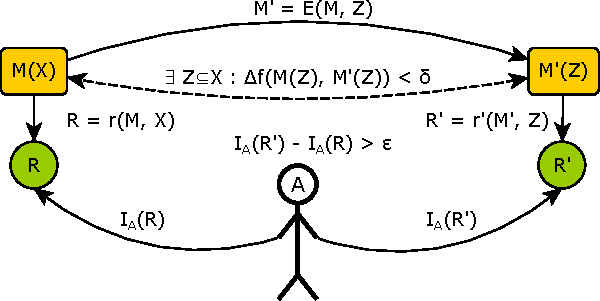
\includegraphics[width=.5\linewidth]{figures/local.pdf}
    \caption{Local explanation and interpretation of a model}
    \label{fig:local}
\end{figure}
%%%%

%---
\paragraph{Local interpretations}
%---

When an observer agent $A$ is \emph{interpreting} a model $M$ behaviour w.r.t.\ some input data $Z \subseteq X$, it is actually trying to assign a subjective interpretability value $I_A(R)$ to some representation $R = r(M, Z)$ of choice, aimed at highlighting the behaviour of $M$ w.r.t.\ the data in $Z$.
%
There, $r : \mathcal{M} \times 2^\mathcal{X} \rightarrow \mathcal{R}$ is \emph{representation means}, i.e., a function mapping models into \emph{local} representations w.r.t.\ a particular subset of the input domain, whereas $\mathcal{R}$ is the set of model representations.
%
For instance, in the case $M$ is a classifier, $R$ may be a graphical representation of (a portion of) the decision boundary/surface for a couple of input features.

There may be more or less interpretable \emph{representations} of a particular model for the same observer $A$.
%
Furthermore, representations may be either global or local as well, depending on whether they represent the behaviour of the model for the whole input space, or for just a portion of it.
%
For example, consider the case of a plot showing the decision boundary of a neural network classifier.
%
This representation is likely far more interpretable to the human observer than a graph representation showing the network structure, as it synthesise the global behaviour of the network concisely and intuitively.
%
Similarly, saliency maps are an interpretable way to \emph{locally} represent the behaviour of a network w.r.t. some particular input image.
%
So, a way for easing interpretation for a given model behaviour w.r.t.\ a particular sort of inputs is about looking for the right representation in the eyes of the observer.

%---
\paragraph{Local explanations}
%---

Conversely, when an observer $A$ is \emph{explaining} a model $M$ w.r.t.\ some input data $Z \subseteq X$, it is actually trying to produce a model $M' = E(M, Z)$ through some function $E: \mathcal{M} \times 2^\mathcal{X} \rightarrow \mathcal{M}$.
%
In this case, we say $M'$ is a \emph{local explanation} for $M$ w.r.t.\ to $Z$.
%
We also say that $M'$ is produced through the explanation strategy $E$.

Furthermore, we define an explanation $M'$ as \emph{admissible} if it has a valid fidelity w.r.t.\ the original model $M$ and the data in $Z$---where $Z$ is the same subset of the input data used by the explanation strategy.
%
More precisely, we say $M'$ is $\delta$-admissible in $Z$ w.r.t.\ $M$ if $\Delta f(M(Z), M'(Z)) < \delta$.

Finally, we define an explanation $M'$ as \emph{clear} for $A$, in $Z$, and w.r.t.\ the original model $M$, if there exists some representation $R' = r(M', Z)$ which is more interpretable than the original model representation $R$.
%
More precisely, we say $M'$ is $\varepsilon$-clear for $A$, in $Z$, and w.r.t $M$ if $I_A(R') - I_A(R) > \varepsilon$ for some arbitrarily big threshold $\varepsilon > 0$.

Several \emph{explanations} may actually be produced for the same model $M$.
%
For each explanation, there may be again more or less interpretable \emph{representations}.
%
Of course, explanations are useful if they ease the seek for more interpretable representations.
%
Thus, providing an explanation for a given model behaviour w.r.t.\ a particular class of inputs is about creating \emph{ad-hoc} metaphors aimed at easing the observer's understanding.

%%%%
\begin{figure}
    \centering
    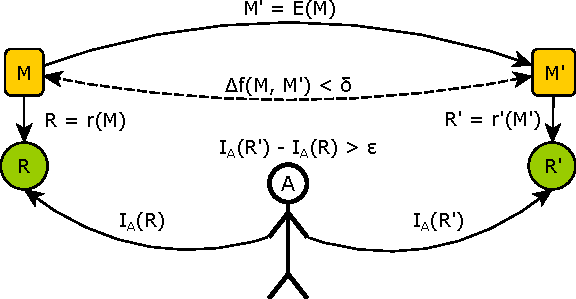
\includegraphics[width=.5\linewidth]{figures/global.pdf}
    \caption{Global explanation and interpretation of a model}
    \label{fig:global}
\end{figure}
%%%%

%---
\paragraph{Global / local explanations}
%---

The theoretical framework described so far -- which is graphically synthesised in \cref{fig:local} -- is aimed at modelling \emph{local} interpretations and explanations, that are, the two means an explanator agent may exploit in order to make AI tasks' \emph{outcomes} more understandable in the eyes of some explanee.

Conversely, when the goal is not to understand some model outcome, but the model itself, from a \emph{global} perspective -- or, equivalently, when the goal is to understand the model outcome w.r.t the whole set of input data $X$ --, the theoretical framework described so far is simplified as shown in \cref{fig:global}, where the dependency on the input data is omitted from functions $E$, $\Delta f$, and $r$.
%
This is possible because we consider the global case as a particular case of the local one, where $Z \equiv X$.

Finally, we remark that the case where a model $M$ is to be understood on a single input-output pair, say $x$ and $y = M(x)$, is simply captured by the aforementioned local model, through the constraint $Z = \{ x \}$ and $M(Z) = \{ y \}$.

%-------------------------------------------------------------------------------
\subsection{Discussion}
%-------------------------------------------------------------------------------

Our framework is deliberately abstract in order to capture a number of features we believe to be essential in XAI.
%
First of all, our framework acknowledges -- and properly captures -- the orthogonality of interpretability w.r.t.\ explainability.
%
This is quite new, indeed, considering that most authors tend to use the two concepts as if they were equivalent or interchangeable.

Furthermore, our framework explicitly recognises the \emph{subjective} nature of interpretation, as well as the subtly \emph{objective} nature of explanation.
%
Indeed, interpretation is a subjective activity directly related to agents' perception and SoM, whereas explanation is an epistemic, computational action which aims at producing a high-fidelity model.
%
The last step is objective in the sense that it does not depend on the agent's perceptions and SoM, thus being reproducible in principle.
%
Of course, the \emph{effectiveness} of an explanation is again a subjective aspect.
%
Indeed, a clear explanation (for some agent) is a more interpretable variant of some given model---thus, the subjective activity of interpretation is again implicitly involved.

The proposed framework also captures the importance of representations.
%
This is yet another degree of freedom that agents may exploit in their seek for a wider understandability of a given model.
%
While other frameworks consider interpretability as an intrinsic property of AI models, we stress the fact that a given model may be represented in several ways, and each representation may be interpreted differently by different agents.
%
As further discussed in the remainder of this chapter, this is far from being an issue.
%
This subjectivity is deliberate, and it is the starting point of some interesting discussions.

Finally, our framework acknowledges the global/local duality of both explanation and interpretation, thus enabling AI models to be understood either general or with respect to a particular input/output pair.

%-------------------------------------------------------------------------------
\subsection{Practical remarks}
%-------------------------------------------------------------------------------

The ultimate goal of our framework is to provide a general, flexible, yet minimal framework describing the many aspects concerning AI understandability in the eyes of a \emph{single} agent.
%
We here illustrate several practical issues affecting our framework in practice, and further constraining it.

According to our conceptual framework, a \emph{rational} agent seeking to understand some model $M$ (or make it understandable) may either choose to elaborate on the \emph{interpretation axis} -- thus looking for a (better) representation $R$ of $M$ -- or it can elaborate on the \emph{explainability axis}---thus producing a novel, high fidelity model $M'$, coming with a representation $R'$ which is more interpretable than the original one (i.e., $R$).

Notice that, in practice, the nature of the model constrains the set of admissible representations.
%
This means that a rational agent is likely to exploit both the explanation and interpretation axes in the general case---because novel representations may become available through an explanation.
%
We argue and assume that each family of AI models comes with just a few \emph{natural} representations.
%
Because of this practical remark, we expect that, in real-world scenarios, an agent seeking for understandability is likely to ``work'' on both the interpretation and the explanation axes.

For instance, consider decision trees, which come with a natural representation as a tree of subsequent choices leading to a decision.
%
Conversely, neural networks can either be represented as graphs or as algebraic combinations of tensors.
%
In any case, neural network models are commonly considered less interpretable than other models.
%
In such situation, a rational agent willing to make a neural network more understandable may choose to combine decision trees extraction (explanation) -- possibly focusing on methods from the literature \cite{AndrewsDT95,xailp-woa2019} -- to produce a decision tree whose tree-like structure (representation) could be presented to the human observer to ease their interpretation.
%
The decision-tree like representation is not ordinarily available for neural networks, but it may become available provided that an explanation step is performed.

Another interesting trait of our framework concerns the semantics of clear explanations.
%
The current definition requires explanation strategies to consume a model $M$ with a given representation $R$ and to produce a high-fidelity model $M'$ for which a representation $R'$ exists, which is more interpretable than $R$.
%
Several semantics may fit this definition.
%
This is deliberate, since different semantics may come with different computational requirements, properties, and guarantees.
%
For instance, one agent may be interested in finding the \emph{best} explanation---that is, the one for which \emph{each} representation is more interpretable than the most interpretable representation of the original model.
%
Similarly, in some cases, it may be sufficient -- other than more feasible -- to find an \emph{admissible} explanation---that is, a high-fidelity model for which \emph{some} representation exists that is more interpretable than \emph{some} representation of the original model.
%
However, the inspection of the possible semantics and their properties falls outside the scope of this thesis and is going to be considered as a future research direction.

\subsection{Assessment of the Framework}\label{sec:validation}

The abstraction level of the presented framework has also been conceived in order to capture most of the current state of the art.
%
Along this line, this section aims at validating the fitting of the existing contributions w.r.t.\ the framework presented in section \cref{ssec:framework}: if our framework is expressive enough, it should allow most (if not all) existing approaches to be uniformly framed, to be easily understood and compared.
%
To this end, we leverage on the work by Guidotti et al.\ \cite{GuidottiMRTGP19}, where the authors perform a detailed and extensive survey on the state-of-the-art methods for XAI, by categorising the surveyed methods according to an elegant taxonomy.
%
Thus, hereafter, we adopt their taxonomy as a reference for assessing our framework.

The taxonomy proposed by Guidotti et al.\ essentially discriminates among two main categories of XAI methods.
%
These are the ``transparent box design'' and the ``black-box explanation'' categories.
%
While the former category is not further decomposed, the latter comes with three more sub-categories, such as ``model explanation'', the ``outcome explanation'', and the ``model inspection''.
%
Notice that, despite the authors' definition of ``explanation'' does not precisely match the one proposed in this chapter, we maintained the original categorisation.

The remainder of this section navigates such a taxonomy accordingly, by describing how each (sub-)category -- along with the methods therein located -- fits our abstract framework.

%-------------------------------------------------------------------------------
\subsubsection{Model explanation}
%-------------------------------------------------------------------------------

The mapping of the methods classified as part of the ``model explanation'' sub-category into our framework is seamless.
%
Hence, it can be defined as follows:
%
\begin{itemize}
    \item[] Let $M$ be a sub-symbolic classifier whose internal functioning representation $R$ is poorly interpretable in the eyes of some explanee $A$, and let $E(\cdot)$ be some \emph{global} explanation strategy.
    %
    Then, the model explanation problem consists of computing some \emph{global} explanation $M' = E(M)$ which is $\delta$-admissible and $\varepsilon$-clear w.r.t.\ to $A$, for some $\delta, \varepsilon > 0$.
\end{itemize}
%
For instance, according to Guidotti et al., possible sub-symbolic classifiers are neural (possibly deep) networks, support vector machines, and random forests.
%
Conversely, explanation strategies may consist of algorithms aimed at
%
\begin{enumerate*}[label=\emph{(\roman{*})}]
    \item extracting decision trees/rules out of sub-symbolic predictors and the data they have been trained upon,
    \item compute feature importance vectors,
    \item detecting saliency masks,
    \item detecting partial dependency plots, etc.
\end{enumerate*}

In our framework, all the algorithms mentioned above can be described as \emph{explanation strategies}.
%
Such mapping is plausible given their ability to compute an admissible, and possibly more explicit models out of black boxes and the data they have been trained upon.
%
However, it is worth to highlight that the clarity gain produced by such explanation strategies mostly relies on the implicit assumption that their output models come with a natural representation which is intuitively interpretable to the human mind.

%-------------------------------------------------------------------------------
\paragraph{Outcome explanation}
%-------------------------------------------------------------------------------

Methods classified as part of the ``outcome explanation'' sub-category can be very naturally described in our framework as well.
%
In fact, it can be defined as follows:
%
\begin{quotation}
    Let $M$ be some sub-symbolic classifier whose internal functioning representation $R = r(M, Z)$ in some subset $Z \subset \mathcal{X}$ of the input domain is poorly interpretable to some explanee $A$, and let $E(\cdot, \cdot)$ be some \emph{local} explanation strategy.
    %
    Then, the outcome explanation problem consists of computing some \emph{local} explanation $M' = E(M, Z)$ which is $\delta$-admissible and $\varepsilon$-clear w.r.t.\ to $A$, for some $\delta, \varepsilon > 0$
\end{quotation}
%
Summarising, while input black boxes may still be classifiers of any sort, explanation, and explanation strategies differ from the ``model explanation'' case.
%
In particular, explanation strategies in this sub-category may rely on techniques leveraging on attention models, decision trees/rules extraction, or well-established algorithms such as LIME \cite{RibeiroSG16}, and its extensions---which are essentially aimed at estimating the contribution of every input feature of the input domain to the particular outcome of the black box to be explained.

Notice that the explanation strategies in this category are only required to be admissible and clear in the portion of the input space surrounding the input data under study.
%
Such a portion is implicitly assumed to be relatively small in most cases.
%
Furthermore, the explanation strategy is less constrained than in the global case, as it is not required to produce explanations elsewhere.

%-------------------------------------------------------------------------------
\paragraph{Model inspection}
%-------------------------------------------------------------------------------

Methods classified as part of the ``model inspection'' sub-category can be naturally defined as follows:
%
\begin{quotation}
    Let $M$ be a sub-symbolic classifier whose available \emph{global} representation $R = r(M)$ is poorly interpretable to some explanee $A$, and let $r(\cdot), r'(\cdot)$ be two different representation means.
    %
    Then, the model inspection problem consists of computing some representation $R' = r'(M)$ such that $I_A(R') > I_A(R)$
\end{quotation}
%
Of course, solutions to the model inspection problem vary a lot depending on which specific representation means $r(\cdot)$ is exploited by the explanator, other than the nature of the data the black box is trained upon.
%
Guidotti et al.\ also provide a nice overview of the several sorts of representations means which may be useful to tackle the model inspection problem, like, for instance, sensitivity analysis, partial dependency plots, activation maximization images, tree visualisation, etc.

It is worth pointing out the capability of our framework to reveal the actual nature of the inspection problem.
%
Indeed, it clearly shows how this is the first problem among the ones presented so far, which only relies on the interpretation axis alone to provide understandability.

%-------------------------------------------------------------------------------
\paragraph{Transparent box design}
%-------------------------------------------------------------------------------

Finally, methods classified as part of the ``transparent box design'' sub-category can be naturally defined as follows:
%
\begin{quotation}
    Let $X \subseteq \mathcal{X}$ be a dataset from some input domain $\mathcal{X}$, let $r(\cdot)$ be a representation means, and let $A$ be the explanee agent.
    %
    Then the transparent box design problem consists of computing a classifier $M$ for which a global representation $R = r(M, X)$ exists such that $I_A(R) > 1 - \delta$, for some $\delta > 0$
\end{quotation}
%
Although very simple, the transparent-box design is of paramount importance in XAI systems as it is the basic brick of most general explanation strategies.
%
Indeed, it may be implicit in the functioning of some explanation strategy $E$ to be adopted in some other model or outcome explanation problem.

For instance, consider the case of a local explanation strategy $E(M, X) \mapsto M'$.
%
In the general case, to compute $M'$, it relies on some input data $X$ and the internal of the to-be-explained model $M$.
%
However, there may be cases where the actual internal of $M$ are not considered by the particular logic adopted by $E$.
%
Instead, in such cases, $E$ may only rely on $X$ and the outcomes of $M$, which are $Y = M(X)$.
%
In this case, the explanation strategy $E$ is said \emph{pedagogical}---whereas in the general case it is said \emph{decompositional} (cf.\ \cite{AndrewsDT95}).

In other words, as made evident by our framework, the pedagogical methods exploited to deal with the model or outcome explanation problems must internally solve the transparent box design problem, as they must build an interpretable model out of some sampled data-set and nothing more.

\section{Symbolic Knowledge Extraction}\label{sec:knowledge-extraction}

\mypapers[section]{xmas-aiiot2019,xaisurvey-ia14,xailp-woa2019}%,shallow2deep-extraamas2021}

Many strategies can be exploited to pursue the purpose of explainability~\cite{GuidottiMRTGP19}.
%
Some authors suggest for instance to \emph{only} rely on \emph{interpretable} algorithms~\cite{Rudin2019} -- such as generalised linear models, decision trees, etc. -- to construct data-driven solutions that are explainable by construction.
%
However, this may hinder predictive performance in the general case, as it essentially cuts off most effective algorithms---e.g., ANN.
%
Another strategy consists of deriving \emph{post-hoc} explanations \cite{KENNY2021103459}, aimed at reverse-engineering the inner operation of a BB so as to make it explicit.
%
In this way, data scientists can keep using prediction-effective predictors such as NN, while still attaining high predictive performance.
%
The focus of this section is on the latter strategy.

Symbolic knowledge extraction (SKE) \cite{GarcezBG01} is among the most promising means to derive \emph{post-hoc} explanations for sub-symbolic predictors.
%
Roughly speaking, the main idea behind SKE is to enable the construction of a \emph{symbolic} surrogate model mimicking the behaviour of a given predictor.
%
There, symbols may consist of intelligible knowledge, such as flat lists or hierarchical trees of \emph{rules}.
%
Such rules can then be exploited to either derive predictions or to better understand the behaviour of the original predictor.

SKE has been applied, for instance, to credit-risk evaluation \cite{baesens2003using,baesens2001building,steiner2006using},  healthcare -- i.e., to make early breast cancer prognosis predictions \cite{franco2007early} and to help the diagnosis and discrimination among hepatobiliary disorders \cite{hayashi2000comparison} or other diseases and dysfunctions \cite{bologna1997three,bologna2000study} --, credit card screening \cite{setiono2011rule}, intrusion detection systems \cite{hofmann2003rule}, and keyword extraction \cite{azcarraga2012keyword}.

\subsection{State of the art}\label{ssec:ske-soa}

Here we discuss the main approaches for extracting symbolic knowledge out of sub-symbolic predictors.

The main underlying assumption behind most works in this category is that, once a sub-symbolic system has been trained over large amounts of data reaching some good predictive performance, then it must have attained a distributed representation of the knowledge contained in the data.
%
Even though unintelligible to human beings, the distributed representation is still somehow buried in the internals of that sub-symbolic systems.
%
Assuming this is the case, then a knowledge extraction technique is a means for making the distributed representation explicit and intelligible.

It is worth to mention that the idea of extracting decision rules or trees from sub-symbolic predictors is not new: it has been introduced several times, in many forms, and with different names and methods, since the late 80s.
%
In fact, generally speaking, systems supporting symbolic knowledge extraction have a number of appealing features.
%
In particular, they support a full exploitation of sub-symbolic techniques, which are the best choice when information must be mined from large amounts of data, and are usually better suited in terms of precision, robustness, and predictive performance.
%
However, thanks to the knowledge extracted, those systems retain desirable XAI-related properties which would otherwise be lost.

Knowledge extraction techniques can be described and discriminated according to a number of orthogonal dimensions, including:
%
\begin{enumerate}
	\item\label{opt:structure-of-knowledge} the structure of the symbolic knowledge they extract (e.g., decision rules, decision trees, etc)
	\item the type of constraints they exploit for decision-making (e.g., linear constraints, M-of-N rules, etc)
	\item\label{opt:sort-of-predictor} the sort of sub-symbolic predictor(s) they can deal with (e.g., neural networks, support vector machines, etc)
\end{enumerate}
%
In the reminder of this section we partition the surveyed works according to dimensions \ref{opt:structure-of-knowledge}, and \ref{opt:sort-of-predictor}, then for each approach we discuss the sort of the constraints exploited.
%
In particular, in the same way as other impactful surveys on the topic \cite{GuidottiMRTGP19,AndrewsDT95}, we distinguish between techniques extracting \emph{rule} lists and techniques extracting decision \emph{trees}.
%
Then, we further distinguish between pedagogical and decompositional approaches.
%
In doing so we borrow the terminology from \cite{AndrewsDT95}, where \emph{pedagogical} techniques are those capable of extracting symbolic knowledge from any sort of sub-symbolic predictor -- as they do \emph{not} exploit any internal detail of the predictor under study to perform the extraction --, whereas \emph{decompositional} techniques are those only capable of extracting symbolic knowledge from some particular sort of sub-symbolic predictor (e.g., neural networks, in most cases)---as they perform the extraction by looking at the internals of the predictor at hand.

%%%%---------------------------%%%%
\subsubsection{Rules extraction}
%%%%---------------------------%%%%

Here we focus on methods for extracting \emph{flat} list of rules in the form
%
\begin{center}
	\textbf{if} $condition_1$ \textbf{then} $outcome_1$
	\\
	\textbf{else if} $condition_2$ \textbf{then} $outcome_2$
	\\
	$\vdots$
	\\
	\textbf{else} $outcome_n$
\end{center}
%
out of sub-symbolic predictors, where each $condition$ is can be a conjunction or disjunction of
%
\begin{inlinelist}
    \item boolean predicates,
    \item linear constraints, or
    \item M-of-N rules
\end{inlinelist}
%
over the attributes of the data used to train the sub-symbolic predictor.


We categorise the surveyed techniques for rule extraction depending on whether they are decompositional or pedagogical;
then we provide some details for each technique;
finally, we analyse them from the XAI perspective in an aggregate manner, given the huge similarity characterising the surveyed techniques from the XAI perspective.

%%%%
\paragraph{Pedagogical approaches}
%%%%

We identified three main pedagogical approaches for rule extraction:
\begin{itemize}
	\item the method from Saito et al.\ (1988) \cite{saito1988}
	\item RxREN (2012) \cite{AugastaK12}
	\item ALPA (2015) \cite{Fortuny2015}
\end{itemize}

In particular, \cite{saito1988} extracts M-of-N rules out of any black-box classifier, regardless of whether it is a neural network or not.
%
Apparently, however, this method does not support regression, and it only supports categorical attributes as conditions in the extracted rules.
%
In spite of its limitations, this work has been proven to be effective in expert systems for diagnosis support.

On the contrary, \cite{AugastaK12} and \cite{Fortuny2015} extract if-then-else rules out of arbitrary classifiers.
%
In particular, RxREN supports datasets with mixed mode attributes (i.e., either categorical or numerical).
%
The algorithm is based on a reverse-engineering algorithm that essentially discards insignificant attributes and discovers the variation range of input attribute for each possible outcome of the classification.
%
For this reason, the rules extracted by RxREN are composed by linear constraints.
%
Conversely, the ALPA rule extraction technique is the first that is applicable to any black-box model with no limitations on the nature of constraints.

It is worth remarking that pedagogical approaches are not based on the structure of the network, therefore they also work with other sub-symbolic models---even though oldest papers tend to mention neural networks more than other sorts of predictors.

Finally, it is worth to be mentioned that pedagogical extraction algorithms can essentially be described as oracle-based algorithms.
%
In fact, in most cases the extraction algorithm works by querying the black box (which is therefore considered as an oracle), and by using the corresponding responses to build the rule list.
%
This behaviour is repeated until the set of rules given by the white-box model converges to that of the black box.
%
In other words, the extraction procedure terminates when the rule set as whole reaches a high \emph{fidelity} w.r.t. the original black box.

%%%%
\paragraph{Decompositional approaches}
%%%%

We identify some main decompositional approaches for rule extraction:
%
\begin{itemize}
	\item RuleNet (1992) \cite{mcmillan1992}
	\item MofN (1992) \cite{towell1992}
	\item the method from Giles et al.\ (1993) \cite{giles1993}
	\item KT (1994) \cite{fu1994}
	\item VI-Analysis (1995) \cite{thrun1995}
	\item RX (1997) \cite{Setiono1997}
	\item the method from N\'u\~{n}ez et al.\ (2008) \cite{NunezAC08}
\end{itemize}

Generally speaking, most approaches here explicitly target a particular sort of sub-symbolic predictor.
%
In particular, all approaches except \cite{NunezAC08} target neural networks, whereas \cite{NunezAC08} target support vector machines (SVM).

Some approaches \cite{mcmillan1992,towell1992,giles1993} exploit some strict assumptions that limit the kind of neural networks they can manage, thus reducing their generality.
%
For instance, the RuleNet technique described in \cite{mcmillan1992} can only handle neural networks aimed at computing endomorphisms on $n$-sized strings of characters, and it aims at making explicit the condition-action rules exploited by such sorts of networks.
%
At the same time, the MofN technique \cite{towell1992} can only handle neural networks attained via the KBANN algorithm described above.
%
As suggested by its name, this method extracts M-of-N-like rules.
%
Finally, the method proposed in \cite{giles1993} focuses on neural networks trained to act as recognisers for regular languages, and it is capable of extracting rules in the form of finite state automata for parsing these languages.

Other approaches -- e.g., \cite{fu1994,thrun1995,Setiono1997} -- target general purpose neural networks.
%
Briefly speaking, they compile networks into sets of rules with equivalent structure.
%
There, each processing unit (neuron) is mapped into a separate rule -- or a small set of rules --, and the in-going connections are interpreted as preconditions to that rule.
%
The particular shape of preconditions -- e.g., linear constraints, M-of-N constraints, etc. --, is then inferred by taking into account the weights of a neuron in-going connections, and its activation function.
%
For instance, the KT algorithm \cite{fu1994} is capable of learning if-then-else rules with linear constraints out of general neural-network classifier.
%
Similarly, the VI-Analysis \cite{thrun1995} and RX \cite{Setiono1997} algorithms perform the same task via different procedures.

Finally, a different and noteworthy approach is described in \cite{NunezAC08}.
%
There, the authors propose a method for extracting if-then-else rules with linear constraints out of SVM classifiers.

\subparagraph{XAI Perspective}

Generally speaking, rule extraction techniques provide \emph{post-hoc} explainability via model simplification.
%
In fact, all the surveyed extraction procedures aims at creating a list of rule having a high-fidelity w.r.t. the source black-box predictor.
%
This rule list can then be considered a symbolic, intelligible explanation of the source predictor.
%
Accordingly, we argue that all these techniques may contribute to the pursuit of XAI goals as: trustworthiness, causality, transferability, informativeness, confidence, and possibly fairness.
%
In fact, by making the inner operation of a black-box predictor explicit and intelligible, these techniques may increase the trustworthiness and confidence of intelligent systems.
%
Furthermore, by providing an overview of the all the possible context-decision situation an intelligent system may face, and by making it possible to inspect which particular rule lead to a particular decision, rule extraction techniques may provide informativeness and causality.
%
Moreover, the symbolic knowledge extracted can be translated into several forms, possibly making it compliant with symbolic intelligent systems.
%
This of course provides for transferability.
%
Finally, rule extraction techniques may help with fairness as well, by highlighting the biases possibly learned by sub-symbolic predictors.

It is worth to mention, however, that rule extraction technique are not the silver bullet of XAI.
%
Issues related to accuracy, fidelity, and consistency, may easily arise in this kind of approaches, because the extracted rule list may not perfectly reflect insights of the original one.
%
We argue that this is essentially unavoidable: the extracted rule lists are essentially approximated models, which are attained by removing (i.e. loosing) information from the source black-box.
%
Moreover, interpretability of the extracted rule list may easily deteriorate as the amount of rules (or the amount of predicates per rule) increases---a situation which may easily arise as the complexity or the dimensionality of the black-box become non-trivial.
%
Finally, it is worth to be noted that virtually all rule extraction techniques only focus on black-box predictors acting as classifiers.
%
Not so much attention has been devoted by the academic community to the extraction of rules out of sub-symbolic regressors, as well as black boxes aimed at performing unsupervised learning tasks.

As a side note concerning SVM-based rule extraction techniques, it is worth to be mentioned that, although they have been known to produce classifiers that are easily comprehensible, they often approximate secondary models of worse accuracy \cite{Barakat2010}.
%
Moreover, even though these models may be reasonably understandable from an expert perspective, they still lack the simplicity and familiarity to an individual user that often intelligent systems have to provide, as in the case of recommendation.

% \subparagraph{Technological Perspective}

% In spite of the many surveyed papers for rule extraction algorithm, only one of them comes with some actual implementation: ALPA.
% %
% The implementation of ALPA is available for download on the web page of the Applied Data Mining Research Group at the University of Antwerp\footnote{\url{http://applieddatamining.com/cms/?q=software}}.
% %
% It consists of a plugin for the Weka data-mining framework\footnote{\url{https://www.cs.waikato.ac.nz/ml/weka}}.
% %
% Thus, it is JVM-based software coming with a detailed manual.
% %
% Apparently, the ALPA source and binary code was published in 2013 and never been updated since then.


%%%%---------------------------%%%%
\subsubsection{Decision trees extraction}
%%%%---------------------------%%%%

Here we focus on methods for extracting \emph{hierarchical} decision tree out of sub-symbolic predictors.

Generally speaking, extracted decision trees are ordinary decision trees whose nodes are represented by rules consisting of a conjunction or disjunction of
%
\begin{inlinelist}
    \item boolean predicates,
    \item linear constraints, or
    \item M-of-N rules
\end{inlinelist}
%
over the attributes of the data used to train the sub-symbolic predictor, similarly to the aforementioned decision rules.
%
In other words, the main difference with decision rules lays in the hierarchical nature of decision choices.

Given the small amount of techniques for decision tree extraction surveyed in this section, we do not split our discussion any further to distinguish between pedagogical or decompositional approaches.
%
Rather we provide this information as part of the detailed description of each method, provided below.
%
We provide a joint discussion of decision tree extraction methods from the XAI perspective, at the end of the paragraph.

\paragraph{Surveyed methods}

We identify three main approaches for decision tree extraction:
%
\begin{itemize}
	\item \textsc{Trepan} (1996, pedagogical) \cite{CravenS95}
	\item the method by Krishnan et al.\ (1999, pedagogical) \cite{KrishnanSB1999}
	\item the method by Schetinin et al.\ (2007, decompositional: random-forest-specific) \cite{schetinin2007}
\end{itemize}

\textsc{Trepan} \cite{CravenS95} is a pedagogical tree extraction algorithm that extracts decision trees from sub-symbolic models.
%
\textsc{Trepan} grows a tree through recursive partitioning, using a best-first expansion strategy, towards M-of-N-like, tree-structured rules.
%
The black box model -- be it a neural network, a support vector machine, or any other model that can be used for classification -- is used as an oracle to answer questions of class belongingness on artificially-generated data points.
%
It also exploits the active learning process to additionally generate data points according to network constraints.

Along the same line, \cite{KrishnanSB1999} proposes decision tree extraction from neural networks.
%
Unlike \textsc{Trepan}, however, the internal structure of the neural network is taken into consideration in the process of decision tree construction.
%
Furthermore, while \textsc{Trepan} leverages on a restricted form of active learning, the method proposed by \cite{KrishnanSB1999} leverages on a genetic algorithm.
%
Finally, it is worth mentioning that the latter algorithm supports the extraction of trees of a given size.
%
In other words, the size of extracted tree can be tuned.

Finally, \cite{schetinin2007} proposes an approach for the probabilistic interpretation of Bayesian decision trees ensembles (a.k.a.\ random forests) as a single decision tree.
%
Classification confidence for each tree in the forest is calculated by exploiting training data: the decision tree covering the maximum number of correct training examples is selected, keeping the amount of classification errors in the remaining examples minimal.
%
Unlike the previous ones, this method of explanation does not extend the input data set with random additional data and cannot be generalised to other types of sub-symbolic black boxes.

\subparagraph{XAI Perspective}

From the point of view of XAI, decision tree extraction methods are quite similar to rule extraction ones, thus similar concerns fit their case.
%
Accordingly, we argue that decision tree extraction techniques provide \emph{post-hoc} explainability via model simplification, and help in pursuing XAI goals such as trustworthiness, causality, transferability, informativeness, confidence, and fairness.

In spite of the many similarities with rule extraction techniques, a remarkable peculiarity of decision trees extractors is worth to be mentioned: as hierarchical models, they are less prone to interpretability issues when the complexity or dimensionality of the source predictor grows.

Other critical aspects remain however unresolved w.r.t.\ rule extraction techniques.
%
These include issues arising from the potential lack of fidelity, as well as the concentration of practically all the decision tree extraction techniques on the sole case of classification tasks---leaving others kinds of tasks in machine learning essentially uncovered.

% \subparagraph{Technological Perspective}

% As far as implementations of decision tree extraction facilities are concerned, we were only able to find an ancient C-based implementation of \textsc{Trepan} on the author's homepage\footnotetext{\url{http://www.biostat.wisc.edu/~craven/TrepanWin.zip}}.
% %
% The archive only contains the C source code of \textsc{Trepan} plus some basic instruction and a \texttt{Makefile} for build automation.
% %
% We classify this technology as a legacy experimental project.

\subsection{A practical framework for MAS}

\mypapers[subsection]{psyke-woa2021}

In the reminder of this thesis, we commit to computational logics as the preferred means for explainability.
%
In particular, we sketch a general framework for XAI, reifying the abstract framework from \cref{ssec:framework} via SKE.

The basic idea is that SKE can be used to draw explanations in the form logic knowledge, which can then be further symbolically manipulated to ease the interpretation of the users.
%
Explanations, in this case, consist of \emph{surrogate} predictors trained to mimic the ones to be explained, as closely as possible.
%
Such surrogates consist of logic knowledge bases, intensively representing the internals of some sub-symbolic ML predictor via interpretable formul\ae{}.
%
In fact, given a trained predictor and a knowledge-extraction procedure applicable to it, the extracted rules/trees act as \emph{explanations} for that predictor -- or as a basis to build some --, provided that they retain high \emph{fidelity} w.r.t.\ both the original predictor and the data used to train it.

\paragraph{Framework design}

\begin{figure}
    \centering
    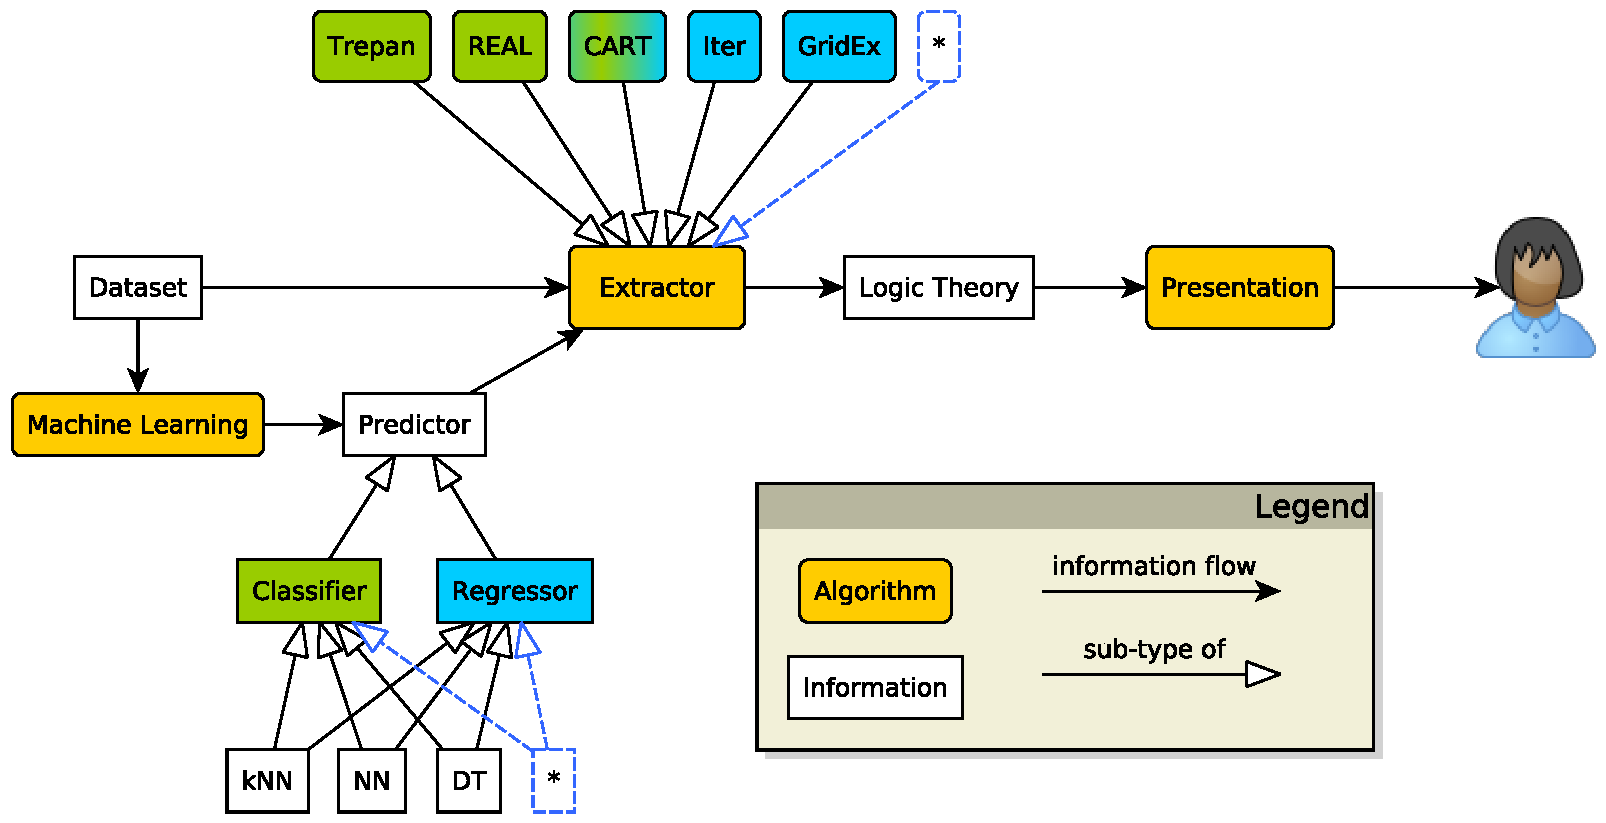
\includegraphics[width=\linewidth]{figures/psyke-abstract.pdf}
    \caption{A practical framework for XAI based on SKE}
    \label{fig:psyke-abstract}
\end{figure}

In particular, as depicted in \cref{fig:psyke-abstract},  a pivotal role in the design of our practical framework is played by the notion of \emph{extractor}, defining the general contract of any knowledge extraction procedure.
%
More precisely, any algorithm accepting a \emph{ML-trained} predictor -- either a classifier or a regressor -- as input, and producing logic rules as output can act as an extractor.
%
Thus, the many algorithms described in \cref{ssec:ske-soa} are well suited to act as extractors.

To perform their job, extractors may require additional information about the data the input predictor has been trained upon.
%
In the general case, such information consists of the data set itself and its schema---i.e., a formal description of the names and the data types of all features characterising the data set itself.
%
Data sets are required to let extraction procedures inspect BB behaviour -- and therefore build the corresponding output rules --, whereas schemas are required to
%
\begin{inlinelist}
	\item let the extraction procedure take informed decisions on the basis of the feature \emph{types},
	\item let the extracted knowledge be clearer by referring to the feature \emph{names}.
\end{inlinelist}
%
For all these reasons, extractors expect a data set and its schema metadata to be provided in input as well.

We stress the logic nature of the extractors' outputs.
%
These may consist of \emph{knowledge bases} containing logic rules expressed via some logic formalism of choice---e.g. FOL, Horn clauses, or ProbLog.
%
These rules should \emph{intensively} represent the general behaviour of the original predictor, in a symbolic way.
%
Furthermore, the actual behaviour of the original predictor on a particular input should be reproducible via inference.
%
Thus, the whole knowledge base acts as a \emph{global} explanation for the original predictor, whereas the proof tree aimed at inferring a particular output acts as a \emph{local} explanation for that particular prediction.

Of course, logic rules may still be poorly interpretable to inexpert human agents.
%
The formalism may for instance be obscure for the human, the rules may be too many, their arity may be too large, or their bodies may involve too many literals.
%
For all these reasons, the framework assumes one further processing step, aimed at representing explanations in the most adequate way for the human agent consuming them.
%
While the possible representations are manifold, the key point here is that the extraction of logic knowledge out of sub-symbolic predictors is not the ultimate step of explanation but rather an intermediate one, enabling the \emph{inspection} of the inner operation of some black-box predictor.

Consider for instance the case of a sub-symbolic predictor $\mathcal{P}$ (say, a neural network) trained on the well-known Iris data-set to classify iris flowers as one of the $\functor{setosa}$, $\functor{versicolor}$, or $\functor{virginica}$ types, by only looking at a flower's sepal width ($SW$) and height ($SH$), and petal width ($PW$) and ($PH$).
%
Suppose that the following logic theory $\mathcal{T}$ is extracted by means of some extraction procedure:
%
\begin{equation*}
    \begin{array}{rcl}
        iris(SL, SW, PL, PW, \functor{setosa}) & \leftarrow & PW \leq 0.65 .
        \\
        iris(SL, SW, PL, PW, \functor{versicolor}) & \leftarrow & PW \in\ ]0.65, 1.64] .
        \\
        iris(SL, SW, PL, PW, \functor{virginica}) & \leftarrow & PW > 1.64 .
    \end{array}
\end{equation*}
%
In the hypothesis that $\mathcal{T}$ has an high fidelity w.r.t. $\mathcal{P}$, the as a whole theory provides useful insights about how it works.
%
For instance, it demonstrates how the ``petal length'' feature plays a central role in the strategy followed by $\mathcal{P}$ to classify iris flowers.
%
Furthermore, given a particular query such as $iris(4.9,\, 2.4,\, 3.3,\, 1,\, C)$, and the proof tree corresponding to a resolution attempt of that query w.r.t $\mathcal{T}$, each query-to-solution path is highly informative:
%
\begin{equation*}
    \resizebox{\linewidth}{!}{
        \begin{prooftree}
            \hypo{\bot\quad\text{(a)}}
            \infer1{C \mapsto \functor{setosa} \quad \cancel{1 \leq 0.65}}
            \hypo{\top\quad\text{(b)}}
            \infer1{C \mapsto \functor{versicolor} \quad 1 \in\ ]0.65, 1.64]}
            \hypo{\bot\quad\text{(c)}}
            \infer1{C \mapsto \functor{virginica} \quad \cancel{1 > 1.64}}
            \infer3{iris(4.9,\, 2.4,\, 3.3,\, 1,\, C)}
        \end{prooftree}
    }
\end{equation*}
%
There, path (a) explains why the iris flower above is \emph{not} of type $\functor{setosa}$ -- i.e., because its petal width (1) is greater than 0.65 --, path (b) explains why it is of type $\functor{versicolor}$ -- i.e., because its petal width is in the $0.65\div1.64$ range --, and path (c) explains why the iris flower is \emph{not} of type $\functor{virginica}$---totally analogous to the $\functor{setosa}$ case.

Finally, more user-friendly representations could be generated for both rules and proof tree paths.
%
The topic is further discussed in \cite{xailp-woa2019}.

\paragraph{Why logic}

The exploitation of computational logic as the basic means to draw explanations is strategical under a number of perspectives.
%
First, we argue that symbolic representations (e.g., the language of FOL formul\ae{}), may act as a \emph{lingua franca} for knowledge representation and exchange among heterogeneous intelligent agents---there including humans.
%
Second, we believe that the adoption of symbolic AI to be an enabling choice for the full exploitation of MAS.
%
Finally, this would enable XAI technologies to benefit form the wide gamma of results, methods, algorithms, and toolkits developed under the umbrella of symbolic AI.

In particular, the potential of logic-based models and their extensions is mainly due to their \emph{declarativeness} and \emph{explicit knowledge representation} -- enabling knowledge sharing at an adequate level of abstraction -- modularity, and separation of concerns \cite{OliyaP2011}---which are especially valuable in open (and possibly distributed) systems composed by several intelligent agents.
%
The interested readers may consider reading \cite{xmas-aiiot2019, expectation-extraamas2021} for a more detailed description of the expected benefits provided by a logic based approach to XAI.

\part{How}
\label{part:how}

\chapter{The Role of Logic Based Technologies}
\label{chap:lbt-role}

\mypapers{logictech-information11}

Artificial intelligence (AI) is getting ever growing attention from both the academia and the industry, in terms of resources, economic impact, available technologies and widespread adoption in virtually any application area.
%
In fact, more and more industries are adopting and applying state-of-the-art AI techniques, to actively pursue challenging business objectives.

Such a general interest, and technology adoption, has been favoured by two main ingredients:
%
\begin{inlinelist}
    \item the development of advanced technologies even at the micro scale, and
    \item the availability of large amounts of data in the environment around us to learn from.
\end{inlinelist}
%
These ingredients have boosted \emph{sub-symbolic} AI techniques, such as machine learning (ML), -- there including deep learning and neural networks -- aimed at exploiting big data to make predictions and take autonomous decisions---in contrast to the more long-established \emph{symbolic} techniques, based on the formal representation of knowledge and its elaboration via explicit reasoning rules.

The increasing role of intelligent systems in human society, however, raises unprecedented issues about the need to \emph{explain} the behaviour, or the result of, intelligent systems---in the sense of being capable of \emph{motivating} their decision and make the underlying decision process \emph{understandable} by human beings: this is where sub-symbolic techniques, despite their efficiency, fall short.
%
This is especially relevant when AI is exploited in the context of human organisations meant at providing public services---such as, e.g., health care / diagnostic systems or legal advice.
%
There is therefore an emerging need to reconcile and synthesise symbolic and sub-symbolic techniques, exploiting the first to \emph{explain} the latter---the scope of \emph{eXplainable Artificial Intelligence} (XAI) \cite{darpa2016-xai}.

So, just when AI's general focus is on sub-symbolic techniques, symbolic approaches are re-emerging as the means to bring AI closer to the human understanding, helping humans to overcome fears and ethical issues by providing explainability, observability, interpretability, responsibility, and trustability.
%
In this context \emph{logic-based} approaches, despite their age, are finding a new youth, for a number of reasons---first of all, because of their closer relation to the human cognitive process.
%
Moreover, their role in (not just computer) science is well understood -- think for instance of the formal study of programs and semantics in computational models, computational logic, inference as computation, logic programming, and automatic theorem proving \cite{gallier2015,boyer2014-computationallogic}.
%
Last but not least, logic-based approaches have long been at the centre of many successful agent-based models and technologies: indeed, agents reason through logic, and plan and coordinate through logical processes \cite{levesque1984,omicini1995,bordini2006}.
%
Overall, from the XAI spark, wider perspectives are raising also beyond the symbolic/sub-symbolic dichotomy, yet all sharing a logic-based root.

Accordingly, in this chapter we focus on the role that logic technologies have played over the years and are going to play in the forthcoming AI landscape---in particular, for the engineering of intelligent systems.
%
We leverage on that analysis to identify the most promising research perspectives and the open issues characterising the current state of the art.

%===============================================================================
\section{Logic-based AI: Application Areas}\label{sec:application}
%===============================================================================

\begin{figure}
    \centering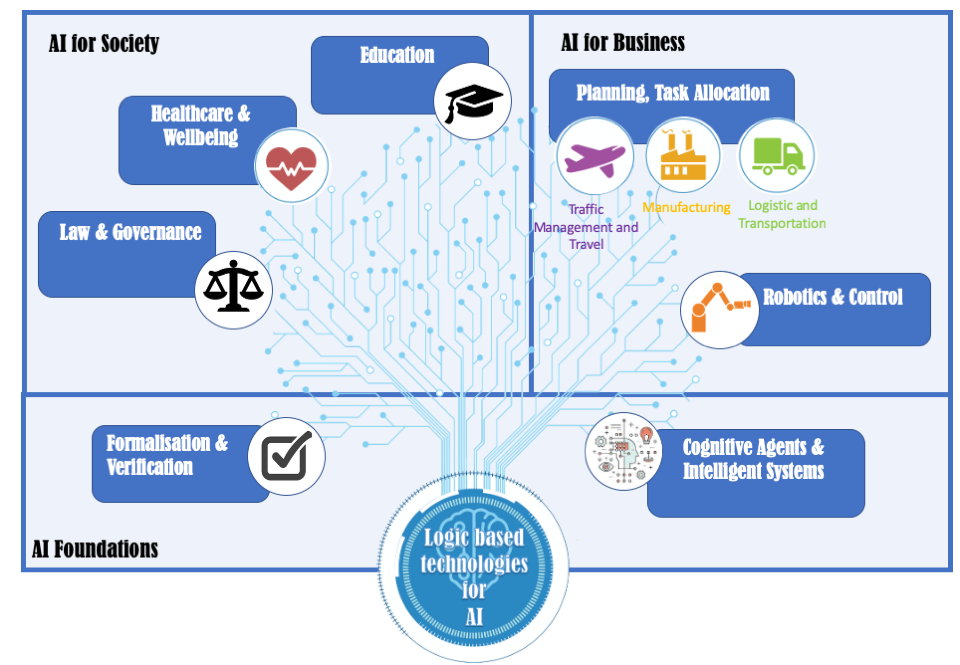
\includegraphics[width=\linewidth]{figures/logicForAI.png}
    \caption[Logic-based technologies application areas w.r.t. main AI categories]{Logic-based technologies application areas with respect to main AI categories---namely, AI Foundations, AI for Society, and AI for Business.  Intentionally, the picture only illustrates the AI areas that are closely related to logic}
    \label{fig:logicBasedAIArea}
\end{figure}

The above techniques have been applied in a variety of fields: \cref{fig:logicBasedAIArea} summarises both the main application areas and their interconnections.
%
For each application area, in the following we
%
\begin{inlinelist}
    \item introduce what the area is about,
    \item outline the main sub-categories (if any),
    \item discuss the role of logic in each sub-category as well as
    \item its benefits and limits, and
    \item present the main actual applications.
\end{inlinelist}

In order to make the comparison actually effective, \cref{tab:logic-usages} and \cref{tab:logic-segments} summarise our findings from two different viewpoints.
The first outlines the strengths of the diverse techniques per application area, that is, where they provide the strongest contribution; the second puts each technique in relation with the different market segments, providing appropriate references to the literature where each technique is used.

%\gcnote{Metto le tabelle qui, spostatele come più vi aggrada}

\newcommand{\y}{\checkmark}

\begin{table}
    \centering
    \begin{tabular}{l||c|c|c|c|c|c|c|c}
        \hline
        & FOL & DL & BDI & TL & FL & PL & DR & CLP \\ \hline
        \hline
        Formalisation \& Verification &    &    &    & \y &    & \y &    &    \\ \hline
        Cognitive Agents              & \y & \y & \y & \y & \y &    & \y &    \\ \hline
        Health-care \& Wellbeing      & \y & \y &    &    &    & \y &    &    \\ \hline
        Law \& Governance             & \y &    &    &    &    &    & \y &    \\ \hline
        Education                     & \y & \y &    &    & \y &    &    &    \\ \hline
        Planning \& Task Allocation   & \y & \y &    &    &    &    & \y & \y \\ \hline
        Robotics \& Control           &    & \y &    & \y & \y &    &    & \y \\ \hline
    \end{tabular}
    \caption{Sorts of logic per application area. Acronym and abbreviation key: FOL: First-Order Logic; DL: Description Logic; BDI: Belief Desire Intention (Logic); TL: Temporal Logic; FL: Fuzzy Logic; PL: Probabilistic Logic; DR: Defeasible Reasoning; CLP: Constraint Logic Programming.}
    \label{tab:logic-usages}
\end{table}

\begin{table}
    \centering
    \resizebox{\linewidth}{!}{
        \begin{tabular}{l||c|c|c|c|c|c|c|c}
            \hline
            & FOL & DL & BDI & TL & FL & PL & DR & CLP \\ \hline
            \hline
            Aerospace                   &     &    &     &    & \cite{castillo2016,ooi2015}   &    &    & \cite{JaffarM94} \\ \hline
            Analytics                   & \cite{Carlsson2012} &    & \cite{Leitao2016} &    &    &    &    &     \\ \hline
            Bioinformatics              & \cite{Carlsson2012} & \cite{yang2003-flora,horrocks2005} &     &    & \cite{torres2006,dong2008}   & \cite{KwiatkowskaNP02} &    & \cite{JaffarM94} \\ \hline
            BPM                         & \cite{Carlsson2012} & \cite{yang2003-flora} &     &    &    &    &    &     \\ \hline
            Constructions               &     &    &     &    &    &    &    & \cite{JaffarM94} \\ \hline
            Critical systems            &     &    &     & \cite{PasareanuVBGMR13, Wu17b} &    &    &    &     \\ \hline
            CPS                         &     & \cite{yang2003-flora} & \cite{Leitao2016,Winikoff2005} & \cite{Holzmann97} & \cite{alam2017,mbuli2017} & \cite{KwiatkowskaNP02} &    & \\ \hline
            Cybersecurity               &     &    &     &    & \cite{goztepe2012,linda2011} & \cite{KwiatkowskaNP02} &    &     \\ \hline
            Databases                   &     & \cite{horrocks2005} &     &    & \cite{kacprzyk2000,kacprzyk1989}   &    &    &     \\ \hline
            Decision support            &     &    &     &    & \cite{liu2009,adriaenssens2004}   &    & \cite{gomez2013}   &     \\ \hline
            Energy                      &     & \cite{lenat1995-cyc} & \cite{Leitao2016} & \cite{Holzmann97} & \cite{suganthi2015}   & \cite{KwiatkowskaNP02} &    & \cite{JaffarM94} \\ \hline
            Finance                     &     & \cite{lenat1995-cyc} &     &    & \cite{bojadziev2007,gil2005}   &    &    & \cite{JaffarM94} \\ \hline
            Government \& Legal         &     &    &     &    &    &    & \cite{prakken2013}   &     \\ \hline
            Hardware                    &     & \cite{lenat1995-cyc} &     &    & \cite{costa1995,bolognani1998}   &    &    & \cite{JaffarM94} \\ \hline
            Healthcare                  &     &    & \cite{Leitao2016,Croatti2019} & \cite{Holzmann97} & \cite{abbod2001,yuan2012}   &    &    &     \\ \hline
            Information retrieval       &     & \cite{horrocks2005} &     &    & \cite{gupta2015,horng2005}   &    &    &     \\ \hline
            %Legal                       &     &    &     &    &    &    &    &     \\ \hline
            Logistic                    & \cite{Carlsson2012} & \cite{lenat1995-cyc} & \cite{Leitao2016,Winikoff2005} & \cite{Holzmann97} &    &    &    & \cite{JaffarM94} \\ \hline
            Manufacturing               &     &    & \cite{Leitao2016,Winikoff2005} & \cite{Holzmann97} & \cite{azadegan2011,lin2005}
            &    &    &     \\ \hline
            Mechanics                   &     &    &     &    &    &    &    & \cite{JaffarM94} \\ \hline
            Mobile applications         &     &    &     & \cite{KohanYAYMHT16,MartinelliMN18} &    &    &    &     \\ \hline
            Railways                    &     &    &     & \cite{Wu17b} & \cite{sezer2011,skarlatos2004}  &    &    &     \\ \hline
            Telecommunications          & \cite{Carlsson2012} &    &     &    & \cite{ghosh1998,catania1996}   & \cite{KwiatkowskaNP02} &    & \cite{JaffarM94} \\ \hline
            Transports                  &     &    & \cite{Leitao2016} &    & \cite{sarkar2012,quddus2006}   &    &    &     \\ \hline
            Web services                &     & \cite{yang2003-flora,horrocks2005} &     & \cite{DoniniMRT06, ArtziKDTDPE10} & \cite{tran2008,chao2005}   &    &    &     \\ \hline
        \end{tabular}
    }
    \caption{Sorts of logic per market segment. Acronym and abbreviation key: FOL: First-Order Logic; DL: Description Logic; BDI: Belief Desire Intention (Logic); TL: Temporal Logic; PL: Probabilistic Logic; DR: Defeasible Reasoning; CLP: Constraint Logic Programming.}
    \label{tab:logic-segments}
\end{table}
%
%\gcnote{Alcune citazioni come ad esempio \cite{Carlsson2012, Winikoff2005, Holzmann97, Croatti2019, Leitao2016, PasareanuVBGMR13, KohanYAYMHT16, KwiatkowskaNP02, Wu17b, DoniniMRT06, ArtziKDTDPE10, MartinelliMN18, JaffarM94} sono nuove e non sono menzionate nel testo}

%-------------------------------------------------------------------------------
\subsection{AI Foundations}\label{ssec:ai-foundations}
%------------------------------------------------------------------------

%---------------------------------------
\subsubsection{Formalisation \& Verification of Computational Systems}
%---------------------------------------

% What is this area about
Formalisation and verification of computational systems refer to a collection of techniques for the automatic analysis of reactive systems---in particular, safety-critical systems, where subtle design errors can easily elude conventional simulation and testing techniques.

The main logic-based technology exploited in this field is model checking \cite{ClarkeGP2001}---nowadays a standard procedure for quality assurance both because of its cost-effectiveness and of the ease of integration with more conventional design methods.
%
The model checker input is a description of the system to be analysed and a number of properties that are supposed to hold: logic is used both to formalise the system description -- states, transitions, model description, and specifications to be verified -- and to express the behavioural aspects, capturing the key properties of information flow.
%
Accordingly, such descriptions are often expressed in temporal and probabilistic logic (and their extension/variations).
%
%The model checker input is then a (usually finite-state) description of the system to be analysed, and the expected properties in terms of temporal-logic formulas.

% Example and applications
%Application examples (\cref{model-check}) are notably heterogeneous, since model-checking is multidisciplinary and cross-field by its very nature.

% Benefits and Limits
Model checking can provide a significant increase in the level of confidence of a system, enabling system verification a-priori, a-posteriori, and -- what is most relevant nowadays -- at runtime.
%
On the other hand, any validation is, by definition, only as good as the system model itself: so, the validation result strongly depends on the precision of the input model.
%
In addition, model checking can turn out to be unsuitable for data intensive applications, as it increases the number communications.

%---------------------------------------
\subsubsection{Cognitive Agents \& Intelligent Systems}\label{ssec:cognitive-arch}
%---------------------------------------

Cognitive architectures are design methodologies, i.e., collections of knowledge and strategies applied to the problem of creating \emph{situated intelligence}.
%
Here, the main technologies borrow from \emph{multi-agent systems} (MAS), since the cognitive architecture can be considered as the brain of an agent reasoning to solve problems, achieving goals and taking decisions.

Generally speaking, cognitive agents in intelligent MAS straightforwardly exploit the logic-based models and technologies for the rational process, knowledge representation, expressive communication, and effective coordination.
%
Developing an agent means to set up a deduction process: each agent is encoded as a logic theory, and selecting an action means to perform a deduction that reduces the problem to a solution, as in theorem proving.
%
Logic can also be used to represent the agent's surrounding \emph{environment} and the \emph{society} of agents---that is, overall, two of the three key aspects when it comes model the structure and dynamics of non-trivial MAS \cite{soda-aoseI}.

Technologies reflect the above context: many are related to agent programming and reasoning, others to agent reliability and verification.
%
Many others focus on the societal aspect of cognitive architectures, by interpreting society as the ensemble where the collective behaviour of the MAS are \emph{coordinated} towards the achievement of the global system goals.
%
Along this line, \emph{coordination models} glue agents together by governing agent interaction, paving the way towards social intelligence: after the seminal work of Shared Prolog \cite{logictuplespaces-ngc12}, notable examples are \tucson{} \cite{tucson-jaamas2}, \respect{} \cite{respect-scp41}, and AORTA \cite{jensen2014-aorta-emas}.

Within an agent society, agents can enter into argumentation processes to reach agreements and dynamically adapt to changes: so, disputes and conflicts need to be managed in order to achieve a common agreement and establish the winner argument.
%
A number of technologies exist for solving reasoning tasks on the abstract argumentation frameworks \cite{Dung:1995:AAF:220193.220197}.
%
Since problems of this kind are intractable, efficient algorithms and solvers are needed.
%
As discussed in \cite{Gaggl_Linsbichler_Maratea_Woltran_2018}, most solvers are based on logic-based programming or logic frameworks including ASP and SAT-solvers.

Specific technologies exist for dealing with the \emph{environment} abstraction of cognitive architectures, mostly in the \emph{coordination} area.
%
There, coordination/interaction artefacts work as runtime abstractions which encapsulate and support coordination/interaction services, usable as building blocks for designing and governing coordination, collaboration,  competition services inside heterogeneous MASs.
%
\emph{Description spaces with fuzziness} \cite{DBLP:conf/sac/NardiniOV11} and \emph{semantic tuple centres} \cite{DBLP:conf/sac/NardiniVP10} can be read as technologies for \emph{situated interaction \& coordination}, emphasising the \emph{situated} aspect of interaction, i.e., the environment-related aspect.
%
In-between lies \lpaas{} (Logic Programming as a Service), a framework aimed at supporting the distribution of logic knowledge in the environment.
%
There, artefacts work as knowledge repositories (in the form of environment structure and properties) while also embedding the reasoning process (enabled and constrained by the knowledge they embody).

When agents are immersed in a Knowledge-Intensive Environment (KIE), the cognition process goes beyond that of the individual agent, and distributed cognition processes may take place, promoting the idea of \emph{intelligent environment} \cite{distributedcognition-hollan-2000}.
%
In such a way, the environment concept is extended beyond situated action---which, by the way, motivates the inclusion of the semantic web within the macro-area of environmental abstractions.

Moving from \cite{Hendler2001}, the ``Agents \emph{in} the semantic web'' sub-category lists JADL, AgentOWL, and EMERALD, which exploit semantic web technologies to inter-operate.

Hybrid cognitive architectures have recently gained attention to combine symbolic and sub-symbolic (emergent) approaches.
%
Examples are ACT-R \cite{Anderson2003} -- based on the modelling of human behaviour --, CLARION \cite{Sun2005} and LIDA \cite{franklin2006}.

In spite of the simplicity and elegance of the logical semantics in logic-based architectures, some issues do exist.
%
The \emph{transduction} problem \cite{bie2004} has to do with the difficulty of accurately translating the model into a symbolic representation, especially in a complex environment.
%
One more difficulty comes from suitably representing information in such a symbolic form that agents can reason about, with and in a time-constrained environment.
%
Finally, the transformation of percepts may not be accurate enough to describe the environment itself, due to sensor faults, reasoning errors, etc.

%-------------------------------------------------------------------------------
\subsection{AI for Society}\label{ssec:ai-society}
%-------------------------------------------------------------------------------

%---------------------------------------
\subsubsection{Healthcare \& Well-being}
%---------------------------------------

In the healthcare domain, AI typically takes the form of complex algorithms and software systems to emulate human cognition in the analysis of complicated medical data, approximating conclusions without direct human input.
%
The primary aim here is to analyse relationships between prevention or treatment techniques and patient outcomes.
%
AI programs have been developed and applied to practices such as diagnosis processes, treatment protocol development, drug development, personalised medicine, and patient monitoring and care.

In this field, logic is exploited to represent knowledge in a human understandable way, and reason on it via properly-formalised rules---in particular, decision support (symbolic) rules, obtained from domain experts and/or decision models induced from data.

At the same time, symbolic logic scales does not scale easily: knowledge engineers need to extract the logic by interviewing or observing human experts.
%
On the other hand, sub-symbolic techniques such as supervised deep learning scale more easily, but are subject to bias in the training data---and, of course, their outcome cannot be explained.

Here again, the semantic web provides a technical framework for the formal semantic modelling -- i.e. interpretation, abstraction, axiomatisation, and annotation -- of healthcare knowledge in terms of classes, properties, relations and axioms \cite{berners2001semantic}.
%
The semantic web framework for healthcare systems provide notable features:
%
\begin{inlinelist}
    \item semantic modelling of the procedural and declarative healthcare knowledge as ontologies, hence a semantically rich and executable knowledge representation formalism;
    \item annotation -- typically via RDF (Resource Description Framework) -- of healthcare knowledge artefacts guided by the ontological model of the knowledge artefact, so as to characterise the main concepts and relations within the artefact;
    \item representation of different patient data sources in a semantically-enriched formalism, that helps to integrate heterogeneous data sources by establishing semantic similarity between data elements;
    \item semantic interoperability between multiple ontologies, using ontology alignment and mediation methods to dynamically synthesise / shape multiple knowledge resources so as to address all the facets of the specific healthcare problem;
    \item specification of the decision-making logic in terms of symbolic rules, which can be executed using proof engines to infer suitable recommendations/actions;
and
    \item provision of a justification trace of the inferred recommendations, so as to let users understand the rationale of the recommended interventions \cite{Abidi2008}.
\end{inlinelist}

Among the healthcare systems based on reasoning, CARA (Context Aware Real-time Assistant) \cite{yuan2012} aims at providing personalised healthcare services for chronic patients in a timely manner, adapting the healthcare technology so that it fits in both with the normal activities of the elderly and with the working practices of the caregivers.
%
Based on a fuzzy-logic context model and a related context-aware reasoning middleware, CARA provides context-aware data fusion and representation, as well as inference mechanisms that support remote patient monitoring and caregiver notification.

%---------------------------------------
\subsubsection{Law \& Governance}\label{sssec:ai-and-law}
%---------------------------------------

Due to its wide potential impact on society and economy, \emph{AI \& law} is one of today's most relevant research areas.
%
It consists of an interdisciplinary effort combining methods and results from several sources, from deontic logic, norms and agent-based simulation to game theory and norms, normative agents, norms and organisation, norms and trust, norms and argumentation.

Contributions in the field of AI \& law are strongly connected with the aforementioned agents architectures.
%
\emph{Agreement technologies} \cite{ossowski2012}, in particular, is a new vision outlining next-generation, open, distributed systems where interaction between computational agents could be  based on the notion of \emph{agreement}.
%
This calls for
%
\begin{itemize}
    \item a normative context defining the rules of the game, or the ``space'' of agreements that the agents can possibly reach;
    \item an interaction mechanism to establish (first) and enact (then) agreements; and
    \item a joint research effort from several fields -- including, but not limited to, multi-agent systems, semantic technologies, social sciences -- aimed at fruitfully combining results and contributions from all such areas---like, for instance, semantic alignment, negotiation, argumentation, virtual organisations, learning, real time, and others.
\end{itemize}
%
Semantic web standards provide a good basis for representing the knowledge of local agents, the functionalities and everything needed to achieve a goal in agreement with other agents.

However, the formalisms behind these technologies fall short when dealing with the distributed, open and heterogeneous nature of AT systems where agents may have different views of the world and, therefore, mutually-inconsistent knowledge bases.
%
To cope with this issue, new logical formalisms -- specifically aimed at handling situations where pieces of knowledge are independently defined in different contexts -- have been defined, extending classical logics in order to deal with incomplete and \emph{defeasible} knowledge.
%
Logic is thus exploited to represent the knowledge with a high degree of peculiarity (for instance defeasibility, but also the possibility to discern among permission, obligation or beliefs in deontic logic), and to reason over such knowledge.

Many interesting experiments have been performed in this application area.
%
Notable defeasible argumentation implementations, aimed at supporting reasoning and resolve inconsistencies, are Defeasible Logic Programs \cite{garcia2004}, ASPIC \cite{modgil2014}, and ABA \cite{dung2009}.
%
Several other applications use ontologies and legal search engines \cite{solarte2016}, which exploit advanced search technology from AI, data mining, data analytics, ontologies and natural language processing \cite{kerikmae2018}.
%
The main issues that remain unsolved in this area is that a unique and general framework for dealing with norms and argumentative issues is still missing: in fact, most solutions are too narrow in scope, tailored to specific use cases, other than being possibly weak from the software engineering perspective.

In short, logic-based approaches in the legal field \cite{Prakken2015}
%
\begin{itemize}
    \item help formalise legal norms and concepts in a clear and understandable way, thus enabling verification and the detection of
unfair policies, or the violation of essential rights;
    \item support explanatory and arguable decisions in the regulatory context.
\end{itemize}

In general, however, current tools are unable to imitate advanced cognitive processes such as human reasoning, understanding, meta-cognition or the contextual perception of abstract concepts that are essential for legal thinking.
%
Indeed, a lawyer's work is often very complex, implying the management and processing of huge amounts of data, where to find correlations between facts and circumstances, and formulate reasoned opinions and action guidelines taking into account all the applicable rights and obligations.
%
This is why the process of understanding and formulating a decision is mostly creative---the result of a complex cognitive process.


%---------------------------------------
\subsubsection{Education}\label{sssec:ai-and-education}
%---------------------------------------

AI has been part of many e-learning platforms for a long time, with applications ranging from personalised learning, recommendation of resources, automated grading, to prediction of attrition rates---to name just a few.
%
The rapid expansion of the \emph{educational technology} industry is now further pushing and exploiting advanced AI-enabled learning technologies.

Within this area, symbolic AI techniques have been used in adaptive educational systems, such as fuzzy logic, decision tree, etc. there, logic has been mainly applied for knowledge management and recommendation.
%
In some systems, for instance, the focus is on examining and assessing the student characteristics in order to generate students' profiles, to be used for evaluating their overall level of knowledge and, consequently, as a basis for prescribed software pedagogy.
%
Symbolic AI approaches are used to support the diagnostic process, so that the course content can be adjusted to cater each student's needs.
Some of them, in addition, are also used to learn from student's behaviour so as to adjust the prescribed software pedagogy.

Applications are related to semantic web technologies, contextualised to e-learning so as to adapt instruction to the learner’s cognitive requirements in three ways---background knowledge, knowledge objectives and the most suitable learning style \cite{guangzuo2004,sancho2005}.
%
Over the years, fuzzy logic techniques and logic MAS have also been experimented for e-learning purposes.
%
In particular, in \cite{almohammadi2013,chrysafiadi2013}, a fuzzy logic-based system learns the users' preferred knowledge delivery to generate a personalised learning environment; whereas in \cite{gong2006} agents detect, recognise, eliminate, and repair the faults of the e-learning course, keeping the system up \& working, providing robustness.
%
Another interesting application in the domain of formal logic proofs, taken as the base of several further extensions, is the Logic-ITA (Intelligent Teaching Assistant) web-based system \cite{yacef2005}: its purpose is to soothe the issues caused by large classes or distance learning, acting as an intermediary between teacher and students.
%
On the one hand, it provides students with an environment to practice formal proofs, giving proper feedback;  on the other, it allows teachers to monitor the class's progress and mistakes.

Although the impact on classrooms has been relatively minor so far, the potential of AI in education is high and likely to increase, as demonstrated by the many European actions / projects currently in place \cite{pedro2019,tuomi2018}.
%
The main challenges and issues concern the creation of a sustainable educational environment, capable of developing equitable education even for the least developed countries---to be dealt with at the suitable political level.

%-------------------------------------------------------------------------------
\subsection{AI for Business: Automation \& Robotics}
%-------------------------------------------------------------------------------

Automation is probably the earliest and perhaps most impactful application area for AI, as it represents the first step towards machine autonomy.
%
Autonomy, in turn, is highly desirable whenever there is a need of re-designing, re-building, or re-programming machines while the deployment context evolves.
%
\emph{Autonomous} machines differ from \emph{automatic} ones in that designers no longer need to forecast any possible situation, because the machine is programmed for learning or planning.
%
This is particularly interesting in \emph{cyber-physical systems} (CPS) \cite{baheti2011} and \emph{robotics}, where machines have a physical body that makes them capable of affecting (or being affected by) the physical world.

Needless to say, applications of automation and robotics in industry are manifold, and so are the corresponding research lines.
%
In the following we explore the role and impact of logic-based paradigms and technologies in such areas.

%---------------------------------------
\subsubsection{Planning \& Task Allocation}
%---------------------------------------

Planning and scheduling are one of the oldest fields in AI, also related to multi-agents and cognitive architectures: research has mainly to do with the decision making process that determines what, when, where, and how to reach a goal and compute a task.
%
There, logic is exploited to represent the knowledge domain, its constraints, and the reasoning mechanism.

Logic-based scheduling methodologies include \emph{rule-based} approaches and \emph{constraint-guided} search.
%
Rule-based scheduling methods aim to emulate the decision-making behaviour of human schedulers, captured in terms of suitable logic rules.
%
Correspondingly, rule-based systems are typically envisioned as a means to replicate the actions of experienced humans with specific scheduling skills.
%
Unsurprisingly, this is one of the most successful application domains of CLP techniques: the scheduler goal is to identify feasible solutions which balance different constraints or schedule requirements.

Applications spread from manufacturing to traffic scheduling and management (e.g., autonomous vehicles, aircraft, \ldots), up to urban search and rescue activities (e.g., traffic assignment in natural disaster evacuations, \ldots), and many others.
%
A typical example of a constraint-based scheduling application is ATLAS \cite{akbarinia2006}, which schedules the production of herbicides at the Monsanto plant in Antwerp.
%
PLANE \cite{Simonis2001} is another system used at Dassault Aviation to plan the production of the military Mirage 2000 jet and the Falcon business jet: the objective is to minimize changes in the production rate, which has a high set-up cost, while finishing the aircraft just in time for delivery.
%
The COBRA system \cite{Simonis2001} generates work plans for train drivers of North Western Trains in the UK: each week, about 25000 activities need to be scheduled in nearly 3000 diagrams on a complex route network.
%
The DAYSY Esprit project \cite{simonis2000} and the SAS-Pilot program \cite{baues1994} consider the operational re-assignment of airline crews to flights.
%
The STP (Short Term Planning) application at Renault \cite{wallace1996} assigns product orders to factories so as to minimise transportation costs.
%
The MOSES application by COSYTEC \cite{wallace1996} schedules the production of compound food for different animal species, eliminating contamination risks while satisfying customer's demand at the minimal cost.
%
FORWARD \cite{simonis1995} is a decision support system, based on CHIP, used in three oil refineries in Europe to tackle all the scheduling problems occurring in the process of crude oil arrival, processing, finished product blending and final delivery.
%
Finally, Xerox has adopted a constraint-based system for scheduling various tasks in reprographic machines (like photocopiers, printers, fax machines, etc.); the scheduler is supposed to determine the sequence of print making and coordinate the time-sensitive activities of the several hardware modules that make up the machine configuration \cite{bistarelli2001}.

Overall, the CLP approach faces well some of the key issues such as development time, nodes visited in the search tree, number of generated feasible solutions, and efficiency.
%
At the same time, the very nature of such systems mandates for considerable development and tuning effort for each new application, as there is no expert to emulate.
%
More generally, the main two issues are \emph{i)} the lack of a structured way to carry the insight gained from one application to the next, and \emph{ii)} the complexity of generating the symbolic knowledge that fully describes the application domain.

%---------------------------------------
\subsubsection{Robotics \& Control}
%---------------------------------------

Cognitive architectures, planning, and task allocation techniques have been widely applied to robotics and control system: indeed, robotics applications translate the agent abstraction of cognitive architecture into a mechanical robot capable of doing action and taking decision.

Logic in robotics is, much more than elsewhere, tailored to the specificity of the application field, since control mechanisms need to control the robot sensors and actuators, along with all their low-level control software (for instance, robot motion mandatorily requires a set of feedback control primitives in order to keep motion coherent).
%
More generally, control systems are present in lifts, photocopiers, car engines, assembly lines, power stations, etc.

Again, the logic-based approaches (and technologies) that are mostly adopted in this context are CLP, fuzzy logic, and temporal logic: in fact, many works dealing with robotic reasoning \cite{Ferrein2008} exploit languages and technologies detailed in \cref{sec:symbolic-reasoning}.
%
CLP-based applications are typically at the smaller end, where it is still possible to prove that some global properties can be guaranteed with a given control.
%
Thus, CLP is often exploited to build control software for electro-mechanical systems with a finite number of inputs, outputs, and internal states: each component is connected to a small part of the overall system, so its behaviour can be captured quite simply.
%
However, when the system is considered as a whole, the number of global states can become very large: this calls for a smart technology that is able to handle such combinatorial explosion \cite{lytras2008}.

On the other side, many control system have been developed exploiting a fuzzy logic approach for dealing with real data which are sometimes imprecise, uncertain, complex, and with a high degree of randomness.
%
Due to its good tolerance of uncertainty and imprecision, fuzzy logic has gained wide application in the area of advanced control of humanoid robots.
%
For the same reason, fuzzy system are powerful tools to face crucial problems in industrial engineering
and technology, such as risk management or product quality assurance, as well as in intelligent decision support system for adaptive industrial engineering \cite{chilwal2020,rastogi2015,patil2012,zhu2004,center1998}.
%
Also, the hybrid techniques based on the integration of neuro-fuzzy networks, neuro-genetic algorithms, and fuzzy-genetic algorithms are of great importance in the development of efficient algorithms \cite{Tahmasebi2012}.

Temporal logic approaches and technologies have been exploited, e.g., for controlling robot motion or planning activities \cite{finucane2010,fainekos2009}, because of their ability to reason over the time and its change, which makes it possible to build control laws to be verified over the time elapse.
%
This is specially relevant for mobile robots, whose specifications are often temporal---even though time is not necessarily captured explicitly.
%
For example, a swarm might be required to reach a certain position and shape eventually, or maintain a size smaller than a specified value until a final desired value is achieved.
%
Other examples are collision avoidance among robots, obstacle avoidance, and cohesion, which are always required.
%
In a surveillance mission, a selected area needs be visited ``infinitely often'' \cite{Kloetzer2007}.

%===============================================================================
\section{Discussion}
%===============================================================================

The new AI era calls for two fundamentals enabling factors:
%
\begin{inlinelist}
    \item the availability of big computing power even in minimal spaces, and
    \item the availability of huge amounts of context-related data.
\end{inlinelist}
%
Such factors on the one side make it possible to learn from experience, which is the playground of sub-symbolic algorithms; on the other, make logic algorithms, historically used for expert systems and hence very effective as for transparency and explainability, computable \emph{in reasonable time}.

Big data have naturally led sub-symbolic approaches to prevail, because of their effectiveness in elaborating and getting valuable results from context-related data, learning trends and repeating patterns: yet, their inherent black-box nature is a clear issue.
%
This is precisely where the integration with symbolic approaches can naturally provide added-value, complementing symbolic and sub-symbolic approaches with each other.
%
In fact, the two main weaknesses of symbolic approaches concern specifically
%
\begin{inlinelist}
    \item the extraction of context-related knowledge, and
    \item computational complexity---the first being the natural territory of sub-symbolic approaches.
\end{inlinelist}

Computational complexity, in its turn, can be partially addressed thanks to the exponential increase of computational power, by suitably exploiting  parallelism, as well as by re-defining and re-tuning symbolic approaches so as to fit nowadays computing paradigms and architectures.
%---as in the case, for instance, of \lpaas{} \cite{lpaas-tplp18}.
%
However, it still remains an issue in some application contexts, often leading to higher processing costs.
%
An example is propositional interval temporal logics (ITL) \cite{goranko2004}, which provide a natural framework for representing and reasoning about temporal properties, but whose computational complexity constitutes a barrier for extensive use in practical applications.
%
To cope with this issue, several approaches exploit constraints or adopt a locality principle; in other cases, as in DLs, complexity is decreased at the price of a limited expressiveness.
%
For instance, in Bowman and Thompson’s decision procedure for propositional ITL, decidability is achieved by means of a simplifying hypothesis -- the locality principle -- that constrains the relation between the truth value of a formula over an interval and its truth values over initial sub-intervals \cite{holldobler2008}.
%
Tableau-based decision procedures have been recently developed \cite{dellaMonica2013} for some interval temporal logics over specific classes of temporal structures, without resorting to any simplifying assumption.

Parallelism and concurrent programming techniques are another valuable tool to deal with complexity.
%
The computing power of multi-level parallelism (MLP), in particular, constitutes a promising technique to facilitate concurrent programming while delivering performance comparable to that of fine-grained locking implementations---see for instance \cite{larus2007} and \cite{jacobsen2013}.

To recap, due to their strong foundations and features, logic-based technologies have the full potential to power symbolic approaches in such integration, opening intriguing perspectives currently under exploration in many research contexts.
%
%as discussed in \xs{perspective}.
%%
%\xt{logic-usages} and \xt{logic-segments}, in particular, point out the very connections among the diverse logics, their application areas, and market segments.
%%
%\xt{logic-usages} highlights that cognitive agents and robotics are the application areas that exploit the widest spectrum of logic-based approaches, whereas other areas typically rely on a smaller subset.
%%
%Reading the table orthogonally, first-order logic, description logic, and fuzzy logics appear to be the most general purpose ones, the others being more specific.
%%
%In its turn, \xt{logic-segments} puts in evidence that some logics -- such as description logic and fuzzy logics -- are widely used in a variety of market segments, while the same does not hold for other logics, like BDI, defeasible reasoning, and probabilistic logic, thus opening a space of action for their possible expansion.
%%
%BDI and defeasible reasoning, in particular, could effectively help to enable intelligent systems, intended as agents immersed in a continuous collaboration with humans, to behave and reason more  ``like a human''.

Overall, the synergy of symbolic and sub-symbolic approaches appears to be a viable and promising option to face key issues in today's intelligent systems---namely, the need of explainable, responsible, ethical AI.
%
In particular, the adoption of symbolic approaches can help to achieve the key features of e-justice, fairness, ethics and transparency.

\paragraph{The role of technology}

It is worth to be highlighted how in this chapter we mostly focus on the \emph{role} of logic based technologies from an utilitarian perspective, i.e. in terms of what functionalities they may offer and what applicative scenarios they may serve.
%
However, in practice, a key role in the rise (or fall) of a technology lays in a number of technical aspects.
%
These include
%
\begin{inlinelist}
    \item its ease of use,
    \item the problem it solves, as well as
    \item the problems it indirectly helps solving,
    \item how it interoperates with other well established technologies, and therefore
    \item the value it adds to (and receives from) them, other than
    \item its resilience w.r.t. the fast-paced change which is inherent in software technologies---i.e. whether it is actively \emph{maintained} or not.
\end{inlinelist}

To further asses all such aspects, in the next chapter we analyse the state of the art of logic-based technologies from a technical perspective.
%
In doing so, we analyse the maturity, technical reach, and maintenance-level of most relevant logic-based technologies.

\chapter{Technological State of the Art}
\label{chap:tech-soa}

\mypapers{lptech4mas-jaamas35,lptech4mas-aamas2021}

Precisely when the success of artificial intelligence (AI) sub-symbolic techniques makes them be identified with the whole AI by many non-computer-scientists and non-technical media, symbolic approaches are getting more and more attention as those that could make AI amenable to human understanding.
%
Given the current status of AI technologies -- mostly focussed on sub-symbolic approaches successful in well-delimited application scenarios --, a key issue for intelligent system engineering is \emph{integration} of the diverse AI techniques: in software engineering terms, not just how to integrate diverse technologies, but also how to preserve \emph{conceptual integrity} when highly-heterogeneous approaches -- bringing about manifold abstractions of various nature -- are put to work together.

The most straightforward and generally-acknowledged way to address the above issue is by using \emph{agents} and \emph{multi-agent systems} (MAS).
%
Agents and MAS have been at the core of the design of intelligent systems since their very beginning:  their long-term connection with \emph{logic-based technologies} might open new ways to engineer \emph{explainable intelligent systems}.

This is why understanding the current status of \emph{logic-based technologies for MAS} is nowadays of paramount importance and why our work focus on logic-based approaches in MAS: they are to be counted among the most promising techniques for building understandable and explainable intelligent systems.
%
Furthermore, given the unavoidable push towards the exploitation of intelligent applications, focussing on logic-based \emph{technologies} is of strategical importance.
%
Accordingly, understanding and representing the current status of the available logic-based MAS technologies is a key step -- from both an historical and an avant-garde perspective -- to let MAS researchers and practitioners identify the actually usable methods for the engineering of intelligent systems.

To this end, in \cite{lptech4mas-jaamas35} we provide a Systematic Literature Review (\slr{}) driven by the primary research question: ``What is the role played by logic-based technologies in MAS nowadays?''.
%
In particular, the \slr{} aims at understanding which and how many logic-based technologies for MAS can be considered ready enough to face the challenges of modern and future intelligent systems, other than identifying what is missing and what research directions require further attention.
%
Accordingly, the goal is to provide an exhaustive assessment of the available logic-based technologies for MAS, by performing a carefully-designed \slr{} on the subject.

\section{Method}

The \slr{} follows a well-founded, understandable, and reproducible method defining how to find, include/exclude, and analyse papers describing logic-based MAS technologies.
%
It relies on the standard \slr{} method: we carried out a manual retrieval, filtering, analysis, and categorisation of huge number of papers, by repeating 8 queries on 6 search engines (Google Scholar, IEEE Xplore, ScienceDirect, SpringerLink, DBLP, ACM Digital Library) and 5 specific conference/workshop proceedings.
%
To keep a tight focus on the \emph{reproducibility} of the whole process, the methodological approach, and the inclusion/exclusion and analysis criteria are carefully designed and described in detail.
%
In particular, we only included works defining or exploiting some \emph{logic-based MAS technology}.
%
A specific definition of \emph{logic-based MAS technology} is provided as well, explicitly requiring the provable availability of
%
\begin{inlinelist}
    \item a clearly identifiable logic-based MAS-related framework into the literature, and
    %
    \item some actual software reification of that framework.
\end{inlinelist}

%
Out of the retrieves papers, we selected 271 documents and there identified 47 technologies, classified them according to both a MAS and a logic perspective, and analysed from the technology viewpoint.
%
Accordingly, the technologies selected in our SLR are analysed and assessed from two different perspectives -- namely, the MAS and the logical perspective --, thus discussing the specific MAS- and logic-related aspects defined, tackled, or exploited by each technology.
%
Along the MAS perspective, we categorise the selected technologies w.r.t.\ the main MAS abstractions they relate to---agents, societies, environment.
%
Along the logic perspective, we categorise the selected technologies w.r.t.\ the sort of logic they relate to---thus choosing among first-order logic, description logic, BDI logic, etc.
%
Such categorisations reveal an uneven distribution of logic-based technologies along both MAS abstractions and logics, and highlighting research opportunities on abstractions and logics which are currently in an urgent need of technologies---such as the environment abstraction and the defeasible logic.

We also perform a technical assessment of each technology, according to number of technological criteria including, but not limited to,
%
\begin{inlinelist}
    \item source-code organisation,
    %
    \item maintenance status,
    %
    \item target platform(s),
    %
    \item availability of executable as well as documentation,
    %
    \item some technical assessment involving the run of executables and available examples.
\end{inlinelist}
%
Arguably, the analysis enables a detailed discussion on the current state of logic-based MAS technologies---in particular highlighting their state of maintenance.
%
More precisely, we consider technologies as unmaintained based on the last provable edit involving either the technology source code or any of its software artefacts\footnotemark.
%
\footnotetext{Since our original assessment (September 2020), some technologies described as unmaintained reworked their repositories, code and/or documentation---as in the case of DALI (\url{https://github.com/AAAI-DISIM-UnivAQ/DALI}) and MCAPL (\url{https://autonomy-and-verification.github.io/tools/mcapl})}

%-----------------------------------------------------------------------
\section{Detailed Technological Analysis}\label{sec:table-evaluation}
%-----------------------------------------------------------------------

% !TeX root = ../phd-thesis.tex
% \begin{landscape}
\begin{table}
\caption{
	Overview on the selected technologies and their analysis.
	Dashes represent missing values, whereas question marks represent unknown values.
}
\label{tab:tech-data}
\begin{adjustbox}{width=.8\textwidth,center}
\begin{tabular}{c|cccccccc}
\textbf{Name} & \textbf{Fresh.} & \textbf{Code} & \textbf{\makecell{Doc.}} & \textbf{License} & \textbf{Target} & \textbf{Runs} & \textbf{Benchmark} & \textbf{Works} \\
\hline\hline
2APL & 2012 & - & 3 & none & JVM 6,7,8 & Yes & *.mas & Yes \\
\hline
2CL & 2013 & - & 1 & none & JVM 7 & Yes & *.2cl & Yes \\
\hline
3APL & 2007 & - & 4 & none & JVM 6 & No & - & - \\
\hline
Agent-0 & 1993 & 1 & 1 & none & \makecell{(Allegro)\\Common Lisp} & Yes & none & No \\
\hline
AFAPL2 & 2016 & 3 & - & LGPL v2 & JVM & ? & none & ? \\
\hline
AgentOWL$^a$ & 2013 & 3 & 1 & LGPL v2 & JVM 8, 11+ & Yes & \makecell{Compiled\\demo} & No \\
\hline
AIL & 2018 & 3 & 1 & LGPL v3 & JVM 8+ & Yes & *.ail & Yes \\
\hline
ALIAS$^b$ & 2000 & 1 & 1 & none & JVM $\mid$ Prolog & No & - & - \\
\hline
AORTA & 2015 & 4 & - & none & JVM +7 & Yes & *.ail & Yes \\
\hline
ASPARTIX$^c$ & 2018 & - & 1 & MIT & Web Service & Yes & *.dl & Yes \\
\hline
ASPIC & 2019 & 4 & 3 & LGPL v3 & JVM 12+ & Yes & \makecell{Compiled\\demo} & Yes \\
\hline
Astra$^e$ & 2018 & 3 & 5 & GPL v3 & JVM & Yes & \makecell{Provided\\examples} & Yes \\
\hline
ConGolog & - & - & - & ? & ? & ? & ? & ? \\
\hline
DALI & 2018 & 3 & 1 & Apache v2 & SICStus & Yes & ? & ? \\
\hline
DCaseLP / DyLog & 2005 & 2 & 3 & none & JVM & No & - & - \\
\hline
DeLP$^d$ & 2018 & 4 & 3 & LGPL v3 & Web Service & No & - & No \\
\hline
DRAGO & 2006 & 2 & 2 & none & JVM 5+ & Yes & \makecell{Any OWL\\ontology} & Yes \\
\hline
EMERALD$^a$ & 2010 & - & 3 & none & JVM 6+ & Yes & \makecell{Compiled\\demo} & Yes \\
\hline
eXAT & 2012 & 4 & 3 & GPL v3 & Erlang & No & - & No \\
\hline
Go! & 2015 & 2 & - & GPL v2 & ? & ? & ? & ? \\
\hline
GOAL$^e$ & 2019 & 5 & 4 & GPL v3 & JVM 8 & Yes & \makecell{Template\\projects} & Yes \\
\hline
Golog & 1998 & 1 & - & ah hoc & SWI $\mid$ ECLiPSe & Yes & - & ? \\
\hline
IndiGolog & - & - & - & ? & ? & ? & ? & ? \\
\hline
JACK & - & - & 5 & proprietary & JVM & ? & ? & ? \\
\hline
Jadex & 2020 & 5 & 5 & GPL v3 & JVM 8+ & Yes & \makecell{Compiled\\demo} & No \\
\hline
JADL/JIAC & 2018 & 4 & 5 & Apache v2 & JVM 7+ & Yes & \makecell{Provided\\examples} & Yes \\
\hline
Jason & 2020 & 5 & 5 & LGPL v3 & JVM 8+ & Yes & \makecell{Provided\\examples} & Yes \\
\hline
Jason-ER & 2019 & 5 & - & LGPL v3 & JVM 8+ & Yes & \makecell{Provided\\examples} & Yes \\
\hline
jDALMAS & 2016 & 3 & - & none & JVM & No & - & - \\
\hline
LPaaS & 2018 & 5 & 3 & Apache v2 & JVM 8+ & Yes & none & ? \\
\hline
MCAPL & 2018 & 3 & 1 & LGPL v3 & JVM 8+ & No & *.ail & No \\
\hline
MCK & - & - & 3 & none & Web Service & Yes & \makecell{Provided\\examples} & Yes \\
\hline
MCMAS & 2017 & 4 & 3 & none & Native / Linux & Yes & \makecell{From\\manual} & Yes \\
\hline
Mozart & 2019 & 5 & 5 & ad-hoc & Native & Yes & \makecell{Provided\\examples} & Yes \\
\hline
MetateM & 2010 & 2 & 3 & GPL v3 & JVM 6+ & Yes & *.sys & Yes \\
\hline
Onto2Jacamo$^e$ & 2017 & - & 1 & none & JVM & No & - & - \\
\hline
Raspberry & - & - & 1 & none & Native / Linux & Yes & *.rasp & Yes \\
\hline
RML & 2019 & 5 & 3 & Apache 2 & JVM 8+ & Yes & *.rml & Yes \\
\hline
Rodin & 2020 & 4 & ? & none & JVM 8 & Yes & none & ? \\
\hline
SALMA$^f$ & 2016 & 3 & 1 & none & Python & No & - & - \\
\hline
SCIFF & 2008 & 1 & 2 & none & SWI $\mid$ SICStus & Yes & none & ? \\
\hline
SHOP & 2020 & 4 & 2 & MPL & Common Lisp & Yes & ? & ? \\
\hline
Spindle & 2017 & 2 & 4 & GPL v3 & JVM 7+ & Yes & *.dfl & Yes \\
\hline
Teleo-R/QLog & 2019 & 3 & 3 & none & QuProlog & No & - & - \\
\hline
\makecell{TuCSoN / Respect\\ (and variants)} & 2020 & 3 & 3 & LGPL v3 & JVM 8+ & Yes & \makecell{Compiled\\demo} & Yes \\
\hline
TuSoW & 2020 & 5 & - & Apache 2 & JVM 8+ & Yes & none & ? \\
%\hline
%VerICS & 2010 & - & ? & ? & ? & ? & ? & ? \\
\hline\hline
\end{tabular}
\end{adjustbox}

\tiny
%\begin{itemize}\tiny
%    \item[]
    $^a$ depends on some ancient Jade version, which is not provided.
%    \item[]
    $^b$ requires the Jinni Prolog interpreter for Java.
%    \item[]
    $^c$ requires the Clingo solver.
%    \item[]
    $^d$ depends on ancient \tuprolog{} version, which is not provided.
%    \item[]
    $^e$ is a plug-in for (or customisation of) the Eclipse IDE.
%    \item[]
    $^f$ requires ECLiPSe Prolog and the PyCLP Python module.
%\end{itemize}
\end{table}
% \end{landscape}

In this subsection we deepen the analysis of the technologies selected in \cite{lptech4mas-jaamas35}, in order to provide additional insights about research questions.
%
\Cref{tab:tech-data} provides an overview of our analysis.

There, we analyse the selected technologies according to a number of technical dimensions, corresponding to the columns of \cref{tab:tech-data}.
%
In particular:
column \textbf{Fresh.} assesses the \emph{freshness} of each technology, by indicating -- when possible -- the year of the visible update;
column \textbf{Code} provides a qualitative assessment of each technology \emph{code base}, when available;
column \textbf{Doc.} provides a qualitative assessment of each technology \emph{documentation}, when available;
column \textbf{License} indicates under which license each technology is provided, if any;
column \textbf{Target} reports on the target \emph{runtime platform(s)} each technology can be executed upon;
column \textbf{Runs} shows our success in \emph{executing} each technology -- or loading it into its target runtime --, possibly after any necessary compilation step;
column \textbf{Benchmark} points out whether each technology is distributed with some \emph{benchmarks} or \emph{examples};
column \textbf{Work} points out whether each technology \emph{works}, i.e., if the aforementioned benchmarks / examples can be executed successfully.

More precisely, the freshness of a technology is defined by the \emph{year} of its most recent release, or, source code modification.
%
The code-base assessment consists of a (possibly missing) integer number ranging from $1$ to $5$:
%
\begin{itemize}
    \item ``$1$'' means the code base is available as a bare archive, even if it appears to have no clear file organisation, and it is comes with no facility supporting the compilation (or, in general, usage) of the code;
    \item ``$2$'' means the code base is available as a bare archive, and it adheres to a well organised structure or it includes instructions on how to compile/use it
    \item ``$3$'' means the code base is available through some version control system \footnote{e.g., SVN, Git, Mercurial, etc.} (VSC, henceforth), but poor support is provided for compilation or usage;
    \item ``$4$'' means the code base is available through some VCS and it comes with some build automation tool\footnote{e.g., Make, Apache Ant, Apache Maven, Gradle, Pip, Npm, etc.} as well, supporting compilation or usage;
    \item ``$5$'' means the code base is available through some VCS, it comes with some build automation tool, and it is also distributed through some official repository;
\end{itemize}
%
whereas a missing value denotes that no assessment can be drawn given the available information---e.g., because we were not able to access any code base.

Similarly, the documentation assessment consists of a (possibly missing) integer number ranging from $1$ to $5$ as well.
%
In this case, however:
%
\begin{itemize}
    \item ``$1$'' means that the only available form of documentation is some textual note briefly describing the technology or how manage the codebase;
    \item ``$2$'' means that some \emph{structured} form of documentation exists describing the technology or how manage the codebase;
    \item ``$3$'' means that a \emph{detailed manual} or some \emph{API reference} are available, but \emph{not both};
    \item ``$4$'' means that \emph{both} a detailed manual and some API reference are available;
    \item ``$5$'' means that a detailed manual, some API reference, and some \emph{usage examples} or \emph{tutorials} are available;
\end{itemize}
%
whereas a missing value denotes the total lack of any form of documentation.

Whenever available, the license of each technology is referenced in \cref{tab:tech-data} as well, possibly leveraging on well-known license acronyms.
%
For instance, as far as open source licenses are concerned, ``GPL'' refers to the GNU General Public License\footnote{\url{https://www.gnu.org/licenses/gpl-3.0.html}, last accessed in April 2020.}, ``LGPL'' refers to the GNU \emph{Lesser} General Public License\footnote{\url{https://www.gnu.org/licenses/lgpl-3.0.html}, last accessed in April 2020.}, ``MIT'' refers to the MIT License\footnote{\url{https://opensource.org/licenses/mit-license.php}, last accessed in April 2020.}, ``MPL'' refers to the Mozilla Public License\footnote{\url{https://www.mozilla.org/en-US/MPL/2.0}, last accessed in April 2020.}, whereas ``Apache'' refers to the Apache License\footnote{\url{https://www.apache.org/licenses/LICENSE-2.0}, last accessed in April 2020.}.
%
The absence of licenses for a particular technology is pointed out as well, as it may have an impact on its users\footnote{\url{https://choosealicense.com/no-permission}, last accessed in April 2020.}.

The target runtime platform is another relevant aspect we analyse for each technology.
%
It provides an intuition of which sorts of machines and devices could in principle be capable of running a given technology.
%
As it clearly emerges from \cref{tab:tech-data}, the \jvm{} platform is targeted by most technologies.
%
This is why, in the particular case of \jvm{}-based technologies, we try to assess the specific version(s) of the \jvm{} they can run upon.
%
Thus, the ``\jvm{} $N$+'' notation indicates that a given technology is tested on all \jvm{} versions ranging from $N$ (included) to version 13 (included) -- which is the most recent one at the time of writing --, and only executes without errors starting from version $N$.
%
Of course, the \jvm{} is not the only platform our selected technologies leverage upon.
%
Some technologies require a compilation step targeting some \emph{native} platform.
%
So, for instance, in case only the \textit{OS} operative system is supported, we write ``Native / \textit{OS}'' to identify the target platform.
%
Other technologies target the Common Lisp, Python, or \erlang{} runtimes, which come with several implementations supporting mainstream operative systems, similarly to what \jvm{} does.
%
%There exist also technologies targeting specific, well-known, implementations of Prolog, such as SWI-Prolog, \sicstus{} Prolog, or ECLiPSe-Prolog.
%%
%In this case we simply write a short indicator of the target Prolog implementation (``SWI'', ``\sicstus{}'', or ``ECLiPSe''), or some piped-separated combination of two or more indicators, in case more than one implementation are supported.
%
Furthermore, a few technologies are available as web services.
%
In those cases, we argue that the actual platform of the service implementation is not essential---this is why we simply denote the target platform as ``Web Service''.
%
Finally, there are some technologies which are explicitly aimed at extending (or customising) the Eclipse IDE
\footnote{\url{https://www.eclipse.org/ide}, last accessed in April 2020}, and are not meant to be used otherwise.
%
In those cases, we indicate ``\jvm{}'' as the target platform, and tag the technology through an \emph{ad-hoc} footnote.

In order to test whether a technology runs or not, we simply launch it on its target platform---possibly, after performing all necessary compilation/confi\-guration steps.
%
If neither compilation/configuration nor launching produces error or crash, then we say the technology runs, otherwise it does not.
%
Thus, a question mark in \cref{tab:tech-data} in the \textbf{Runs} column may indicate either the total lack of any information on how to launch the technology, or, the impossibility of producing / accessing an executable to launch.

Finally, when we are able to run a given technology, we then test it to get further detail, so as to understand if it actually \emph{works} or not.
%
To do so, we first look for available \emph{benchmarks} or examples into the running technologies code bases, documentation, or home pages.
%
In case some benchmarks / example are available, we check if they can be run without producing error outputs or crashes.
%
If they can, then the technology works, otherwise it does not.
%
Thus, a missing value in \cref{tab:tech-data} in the \textbf{Benchmark} or \textbf{Works} columns indicates that no assessment is needed because the technology does not run.
%
Conversely, a question mark in the same columns denotes the impossibility to perform any further assessment due to lacking benchmarks, examples, or instructions on how to launch them.

%%%%
% !TeX root = ../phd-thesis.tex
\begin{table}
\caption{Statistics on selected technologies}
\label{tab:tech-stats}
\centering
\begin{tabular}{l||ccc}
\multicolumn{1}{c}{\textbf{}} & \textbf{Absolute} & \textbf{Relative} & \textbf{Meaning}                              \\
\hline\hline
N. selected tech              & 47                & 100\%             &                                               \\
\hline
Maintained since 2019         & 12                & 25.53\%           & Fresh. $\geq$ 2019                            \\
\hline
Maintained since 2018         & 20                & 42.55\%           & Fresh. $\geq$ 2018                            \\
\hline
Open source                   & 26                & 55.32\%           & License $\not\in \{ \text{none}, \text{?} \}$ \\
\hline
Unlicensed                    & 19                & 40.43\%           & License $=$ none                              \\
\hline
JVM-based                     & 30                & 63.83\%           & Target starts with JVM                        \\
\hline
Certainly runs                & 31                & 65.96\%           & Runs $=$ yes                                  \\
\hline
Certainly works               & 21                & 44.68\%$^a$       & Works $=$ yes                                 \\
\hline
Codebase quality              & 16                & 34.04\%           & Code $\geq$ 4                                 \\
\hline
Documentation quality         & 9                 & 19.15\%           & Doc. $\geq$ 4                                 \\
\hline\hline
\end{tabular}
\begin{itemize}
	\item[] $^a$ corresponding to 67.74\% of the technologies which certainly run.
\end{itemize}
\end{table}
%%%%

By aggregating the data in \cref{tab:tech-data}, we can draw several interesting conclusions.
%
Most relevant ones are summarised in \cref{tab:tech-stats}.
%
The most evident information is that only 12 out of 47 technologies have been actively maintained since 2019---i.e., 25.53\% of the total.
%
The percentage is lower than 50\%, even if we enlarge the spectrum to technologies maintained since 2017.
%
However, most technologies (65.96\%) can still be run successfully -- regardless of when they were last updated --, even though we are able to make them work in 67.74\% of cases only.

Another interesting trait is that -- except for \jack{} -- all technologies that are explicitly licensed come with an open source license.
%
These correspond to 55.32\% of the total.
%
The amount of unlicensed technologies is quite high as well, as it corresponds to the 40.43\% of the total.

It is interesting to note how the \jvm{} is by far the preferred platform for logic-based MAS technologies.
%
Indeed, 63.83\% of the selected technologies target some version of the \jvm{}.
%
Other recurring platforms are Lisp-, Prolog-, or native-based.

Finally, it is worth to be mentioned how -- except for a few notable exceptions, such as \jason{} -- poor care is given to technologies code bases and documentary resources.
%
Indeed, considering the 1-5 ranges defined above, only 34.04\% of the technologies come with a code base whose quality is greater than 3, whereas only 19.15\% are scored similarly as far as documentation is concerned.

%\note{A chapter on the state of Prolog systems?}

%%===============================================================================
\section{Main Outcomes}\label{sec:outcomes}
%%===============================================================================

The outcome of the \slr{} highlights that, as far as logic-based technologies for MAS are concerned, there is still room for technological advancements---except for a few relevant success stories.
%
In fact, despite the enormous technological effort clearly carried out by the MAS community in the last decades, several surveyed technologies cannot be considered as mature and ready for use in the new challenging contexts required by AI.
%
Several technologies are in fact unmaintained, outdated, or just proof of concepts.

In our original work the discussion attempts to provide a comprehensive answer to all the \slr{} research questions.
%
In the following we summarise some general remarks in relation to key features of modern intelligent systems, namely:
%
\begin{inlinelist}
    \item inherent distribution and decentralisation and deep entanglement with domains like the Internet of (Intelligent) Things (Io(I)T) and Cyber-Physical Systems (CPS);
    %
    \item support to key properties such as robustness, efficiency, interoperability, portability, standardisation, situatedness, and real-time support;
    %
    \item need to reconcile and synthesise symbolic and sub-symbolic AI, exploiting the former to \emph{explain} the latter so as to overcome fears and ethical issues posed by AI by providing for explainability, observability, interpretability, responsibility, and trustability---the scope of XAI.
\end{inlinelist}

%----
\subsubsection{Applicability to distributed domains such as \iot{} and CPS}
%----

The existing agent-oriented logic-based solutions applicable to the \iot{} and CPS are only available for a specific and limited set of devices and platforms.
%
For instance, Agent Factory Micro Edition (AFME) \cite{afme-iccs2006} enables the execution of a deliberative agent on top of mobile phones with CLDC/MIDP profiles and Sun-SPOT sensor by means of TCP/IP and Zigbee protocols.

However, some technologies, more than others, are explicitly designed to support \iot{} domains and CPS.
%
For example, the \lpaas{} architecture \cite{lpaas-tplp18} is designed to promote distributed intelligence for the \iot{} world---offering logic programming as a service, and explicitly addressing the requirements and issues of cloud and edge architectures.
%
Analogously, the situated coordination approach promoted by the \tucson{}/\respect{} model and technology can be explicitly exploited to handle situatedness in MAS as a coordination issue.
%
Also, \tucson{} \cite{tucson-jaamas2} provides the main abstractions for \iot{} environments: environmental resources can be sources of perceptions (like sensors), targets of actions (like actuators), or even both.

Finally, there are technologies that are not explicitly meant to address the \iot{} and CPS domains, but still let us suppose they would be easily portable to those domains---because of their standard compliance, interoperability, and portability features.
%
Among the many, \jason{} \cite{jason-clima2005} supports interoperability with non-\jason{} agents via \jade{} \cite{jade-mapbook2005} through \fipa{}-ACL communication \cite{fipa-acl}.
%
Similarly, there are extensions to \jack{} \cite{jack-mapbook2005} that make it work in open systems.
%
Finally, the Teleo-Reactive \cite{nilsson2001-teleoreactive} approach has been often exploited to facilitate the development of the \iot{} systems as a set of communicating Teleo-Reactive nodes.

%----
\subsubsection{Symbolic and sub-symbolic integration}
%----

With respect to the need to reconcile and integrate symbolic and sub-symbolic techniques, none of the selected technologies has been experimented yet \cite{xaisurvey-ia14}, due to their original design purpose out of this scope.
%
However, we argue that portable and interoperable technologies might be more suitable for the integration.
%
Anyway, the field is still unexplored and represents a frontier research domain.

%----
\subsubsection{Can existing technologies be labelled as ready? If not, what is missing?}
%----

The role of logic-based technologies in MAS nowadays exhibits a huge potential for covering the vast majority of intelligent system abstractions.
%
However, just a few among the technologies surveyed can be actually labelled as \emph{ready-to-go}, in particular when considering the new challenges for symbolic technologies in AI.

Even though 10\% of the selected technologies can be considered as mature -- in terms of cross-platform support, code quality, and ease of distribution in heterogeneous environments --, most of the times they have not been tested in pervasive and real-world scenarios, yet.
%
This implies, at least, that further research and technical activity are required to ensure that any technological barrier can be overcome.
%
Furthermore, integration with sub-symbolic techniques remains a \emph{nice-to-have} feature, but it is not actually a thing in any MAS technology, for the time being.
%
Nevertheless, the selected technologies are an excellent starting point for
%
\begin{inlinelist}
    \item highlighting the advantages of logic-based technologies, and
    \item broadening the scope of research towards the directions envisioned.
\end{inlinelist}

%In the end, we forward the interested readers to the original SLR for the full details \cite{lptech4mas-jaamas35}.

%\section{Current State of Logic-Based Technologies}

%\cite{lptech4mas-aamas2021}
%\cite{lptech4mas-jaamas35}
%\cite{logictech-information11}

%\section{Current State of Machine Learning Technologies}

%\section{Current State of XAI Technologies}

%\cite{xaisurvey-ia14}

%\chapter{Need for An Open Ecosystem for Logic-Based AI}
%
%\cite{cco-softwarex-2021-2pkt}

\section*{The Need for Interoperability}

%\note{Link next chapter}

Our survey identifies two major lack in the logic-based technology playground, namely \emph{maintenance} and \emph{interoperability}.

Maintenance (and its lack) is essentially an organizational aspect concerning individual research groups around the globe.
%
Career incentives within academia discourage the maintenance of software on the long run.
%
So, the current maintenance status of logic-based technologies is unsurprising.
%
In this perspective, we consider as positive that a non-negligible percentage of logic-based technologies has a decades-long life span.

The actual issue we detect through our survey concerns \emph{interoperability} among the logic-based technologies which survived so far.
%
Arguably, this is the most relevant aspect research communities should be concerned by.
%
Existing logic-based technologies often address specific uses cases, or rely upon monolithic runtimes, often targeting single platforms or having inconvenient constraints and dependencies.
%
Poor care is devoted to favour their interoperability and joint exploitation, probably because of the different programming platforms/runtimes they leverage upon, or the use cases they have been designed for.
%
In other words, logic-based technologies are often constructed as technological \emph{silos} -- being so optimised for performance and correctness while being poorly interoperable among each other -- targetting the LP or MAS communities alone.

On the other side, the data science playground is flourishing, also because of the emergent selection few key platforms -- e.g. Python or R -- upon which many inter-dependent and interoperable research project are built, adding value to each other.

Hence, the need for efforts pushing the state of the art of logic-based technologies towards a higher degree of interoperability -- both internally, and with DS technologies -- is compelling.
%
Along this line, in the next chapter, we propose a paradigm shift aimed at satisfying this need.
%
In particular, we propose the design and implementation of a general-purpose \emph{logic-ecosystem}, upon which other logic-based (as well as ML-oriented) technologies can be constructed, embedded, or made interoperable with.
%
Then, in the remainder of this thesis, we discuss how our ecosystem can be designed and extended to cover the need for interoperable technologies at the intersection among symbolic and sub-symbolic AI.

\chapter{The 2P-Kt Ecosystem for Logic-Based AI}
\label{chap:ecosystem}

\mypapers{cco-softwarex-2021-2pkt}

\mystudentsthesis{Master's}{Siboni2019}

While their impact on the \emph{symbolic} branch of AI is well established, many emergent AI techniques leverage logic to make data-driven AI either more predictable or more understandable.
%
This is why the need for solid, interoperable, general-purpose \emph{logic-based technologies} is nowadays more compelling than ever.
%
Most of the logic-based technologies proposed so far are typically either built on top or as extensions of the Prolog language.
%
Even when this is not the case, \emph{monolithic} solutions are built around different inference procedures, unification mechanisms, or knowledge representation techniques.

This chapter stems from the idea that logic-based technologies should be neither constructed as Prolog-centred monoliths nor tailored to a specific semantics or language.
%
Instead, in order to maximise their impact on AI, logic-based technologies should welcome the manifold contributions coming from the LP playground, supporting the exploitation of as many mechanisms as possible, in an unopinionated way.
%
As a foundational step in that direction, we present \twopkt{}, a reboot of the \tuprolog{} project offering a general-purpose, extensible, and interoperable \emph{ecosystem} for logic programming and symbolic AI.

\section{The Need for an Ecosystem}
\label{sec:motivation}

In spite of the wide availability of logics, inference rules, and resolution strategies in the LP literature, only a relatively small amount of them have been reified into actual logic-based technologies.
%
Among these, the Prolog language \cite{ColmerauerR93} is by far the most successful story \cite{logictech-information11}.
%
It consists of a well-defined language \cite{prologISO-pt1,prologISO-pt2} coming with several implementations \cite{homepageBprolog,homepageCiao,homepageEclipse,homepageSicstus,homepageSwi,homepageXsb,homepageTau}.

While standard implementations of Prolog target first-order logic (FOL) via SLDNF inference rule \cite{robinson1965,Kowalski1974,Clark77} and depth-first resolution strategy, most implementers have extended Prolog to support other resolution strategies as well.
%
This is the case of Prolog implementations supporting for instance, \emph{constraint logic programming} (CLP) \cite{jaffar1987}, \emph{constraint handling rules} (CHR) \cite{Fruhwirth98}, \emph{tabled resolution} \cite{SwiftW12}, etc.

Thanks to the versatility of FOL, it is a common practice in LP to either develop logic-based technologies either \emph{on top} of Prolog or \emph{from scratch}.
%
In the former case, the resulting logic-based technologies tend to be poorly interoperable -- as strictly Prolog-dependent \cite{kotlindsi4prolog-woa2020} --, while in the latter case they tend to be very narrow in scope---as heavily tailored on a particular domain.

Building logic-based technologies on top of Prolog is often preferred as they automatically inherit Prolog basic mechanisms, including e.g.\ the capability of
%
\begin{inlinelist}
    \item representing data structures via logic terms,
    \item knowledge via Horn clauses,
    \item logic unification,
    \item efficient in-memory indexing of logic information,
    \item a flexible inference rule, and
    \item meta-level programming.
\end{inlinelist}
%
This is the smartest strategy when novel logic-based technologies must be quickly bootstrapped, yet it may easily result in poorly-interoperable, Prolog-tailored solutions.
%
Conversely, when Prolog capabilities are not adequate for the particular problem at hand, logic-based technologies may be designed from scratch.
%
This commonly involves re-designing and re-implementing most LP features from scratch.

In \cite{Sterling1996}, Sterling states that logic unification is by itself the major contribution of LP to software engineering---thus singling a specific feature out of Prolog for its value and benefits.
%
Along this path, we argue that many aspects of LP may be useful in AI by themselves, and each contribution could be conveniently reified into some individually-usable software library.
%
Accordingly, our work aims at the creation of an \emph{open ecosystem} for interoperable, general-purpose LP libraries, virtually supporting multiple logics, inference rules, and resolution strategies, and possibly factorising any shared aspect---e.g. terms and clauses representation, unification, in-memory storage, (de)serialisation, etc.

In the early 2000s, the idea of LP as a key \emph{technology}-enabler of intelligent application was already in place.
%
The \tuprolog{} project \cite{tuprolog-padl01} was proposed for this purpose.
%
It consists of a lightweight \emph{malleable}, object-oriented, Java-based implementation of Prolog \cite{tuprolog-sac08} which can be used as a library for JVM projects.
%
Despite many versions have been proposed along the years -- bringing new features, or more platforms support \cite{2p-alpnews2013} --, and many research products have been built upon it -- such as \tucson{} \cite{tucson-jaamas2}, \respect{} \cite{respect-scp41}, \lpaas{} \cite{lpaas-bdcc2}, or \tenderfone{} \cite{blockchainmas-applsci10},  \argtwop{} \cite{arg2p-cilc2020}, etc. --, it still consists of a \emph{monolithic} library targetting Prolog \emph{alone}.

Accordingly, this chapter stems from the idea that Prolog is not the silver-bullet for logic-based technologies, and the belief that LP should not be reduced to Prolog alone.
%
For this reason, we present \twopkt{}, a \emph{reboot} of the \tuprolog{} project aimed at providing a common technological ground for LP.
%
Acknowledging that most mechanisms in LP have the potential to be of general value, not necessarily tailored to any specific logic, inference rule, or resolution strategy, \twopkt{} consists of a logic-based \emph{ecosystem} for symbolic AI, designed and implemented by taking openness, modularity, extensibility, and interoperability into account.

More precisely, the \tuprolog{} project has been completely re-designed and re-written, splitting LP functionalities into minimal, loosely-coupled, Prolog-agnostic, individually-usable, multi-platform \emph{modules}.
%
The rationale behind this choice is to enable the incremental addition of novel LP functionalities to the \twopkt{} ecosystem -- possibly targeting other inference rules and search strategies --, minimising duplication of features and reusing pre-existing ones, while supporting as many programming platforms as possible.

On the long run, \twopkt{} aims at becoming a comprehensive technological playground supporting several sorts of logics -- e.g. first-order, higher-order, temporal, deontic, etc. -- and mechanisms---e.g. deductive, inductive, abductive, probabilistic reasoning, etc.

Finally, a non-negligible effort is devoted to keep \twopkt{} widely interoperable at the technological level with as many platforms as possible---to maximise the pool of potential adopters.
%
This is why most \twopkt{} modules are Kotlin Multiplatform projects -- currently supporting the JVM, JS, and Android platforms --  while others are expected to be supported soon---e.g. MacOS, iOS, .NET, and Python.

%\section{Software description}
%\label{sec:sw-description}

%\twopkt{} is deeply rooted in LP, a programming paradigm based on computational logic \cite{lloyd1990computational,Nerode1996}.
%
%In LP, programs are typically \emph{theories} (a.k.a. \emph{knowledge bases}, KB), i.e. collections of sentences in logical form, expressing \emph{facts} and \emph{rules} about some domain.
%%
%These are often in the form of \emph{clauses}, i.e.:
%\[ Head \impliedBy Body_1,\ ...,\ Body_n \]%,
%where both $Head$ and $Body_i$ are \emph{atomic} formul\ae{}, and the whole sentence is read declaratively as logical implication ($Head$ is implied by all $Body_i$).
%%
%If $n = 0$, the clause is called \emph{fact}, \emph{rule} otherwise.
%%
%An atomic formula is an expression in the form $P(t_1,...,t_m)$ where $P$ is a $m$-ary predicate ($m \geq 0$), and $t_1,...,t_m$ are \emph{terms}.
%%
%Terms are the most general sort of data structure in LP languages.
%%
%They can be \emph{constant} (either \emph{numbers} or \emph{atoms}/strings), \emph{variables}, or recursive elements named \emph{structures}.
%%
%Structures are used to represent clauses, lists, sets, or other sorts of expressions.
%
%Logic \emph{solvers} exploit KB to answer users' \emph{queries} via some inference procedure and resolution strategy.
%%
%For instance, Prolog interpreters exploit a \emph{deductive} procedure rooted into the SLDNF resolution principle \cite{Kowalski1974, Clark77}, and a depth-first strategy.
%%
%Yet, other options exist like, e.g., abductive \cite{FungIff97}, inductive \cite{Muggleton94}, probabilistic \cite{RaedtK15}, inference.
%%
%Each of them represents a particular reification of a logic solver.
%
%A common mechanisms in LP is the \emph{unification} algorithm \cite{MartelliMontanari1982} for constructing a \emph{most general unifier} (MGU) for any two suitable terms.
%%
%Provided that such an MGU exists, the subsequent application of the resulting substitution to the terms, renders them syntactically equal.
%%
%This is a basic brick in virtually all LP algorithms, regardless of the particular inference rule.
%
%Summarising, LP leverages several mechanisms -- terms and clauses representation, knowledge base storage, unification, resolution, etc. --, which constitute the basis of any logic solver.
%%
%Subsets of these mechanisms may be useful \textit{per se}.
%%
%\twopkt{} makes all these mechanisms \emph{individually} available, while easing the construction of novel mechanisms on top of the existing ones.

\section{Overall Design}
\label{ssec:sw-architecture}

\begin{figure}
    \centering
    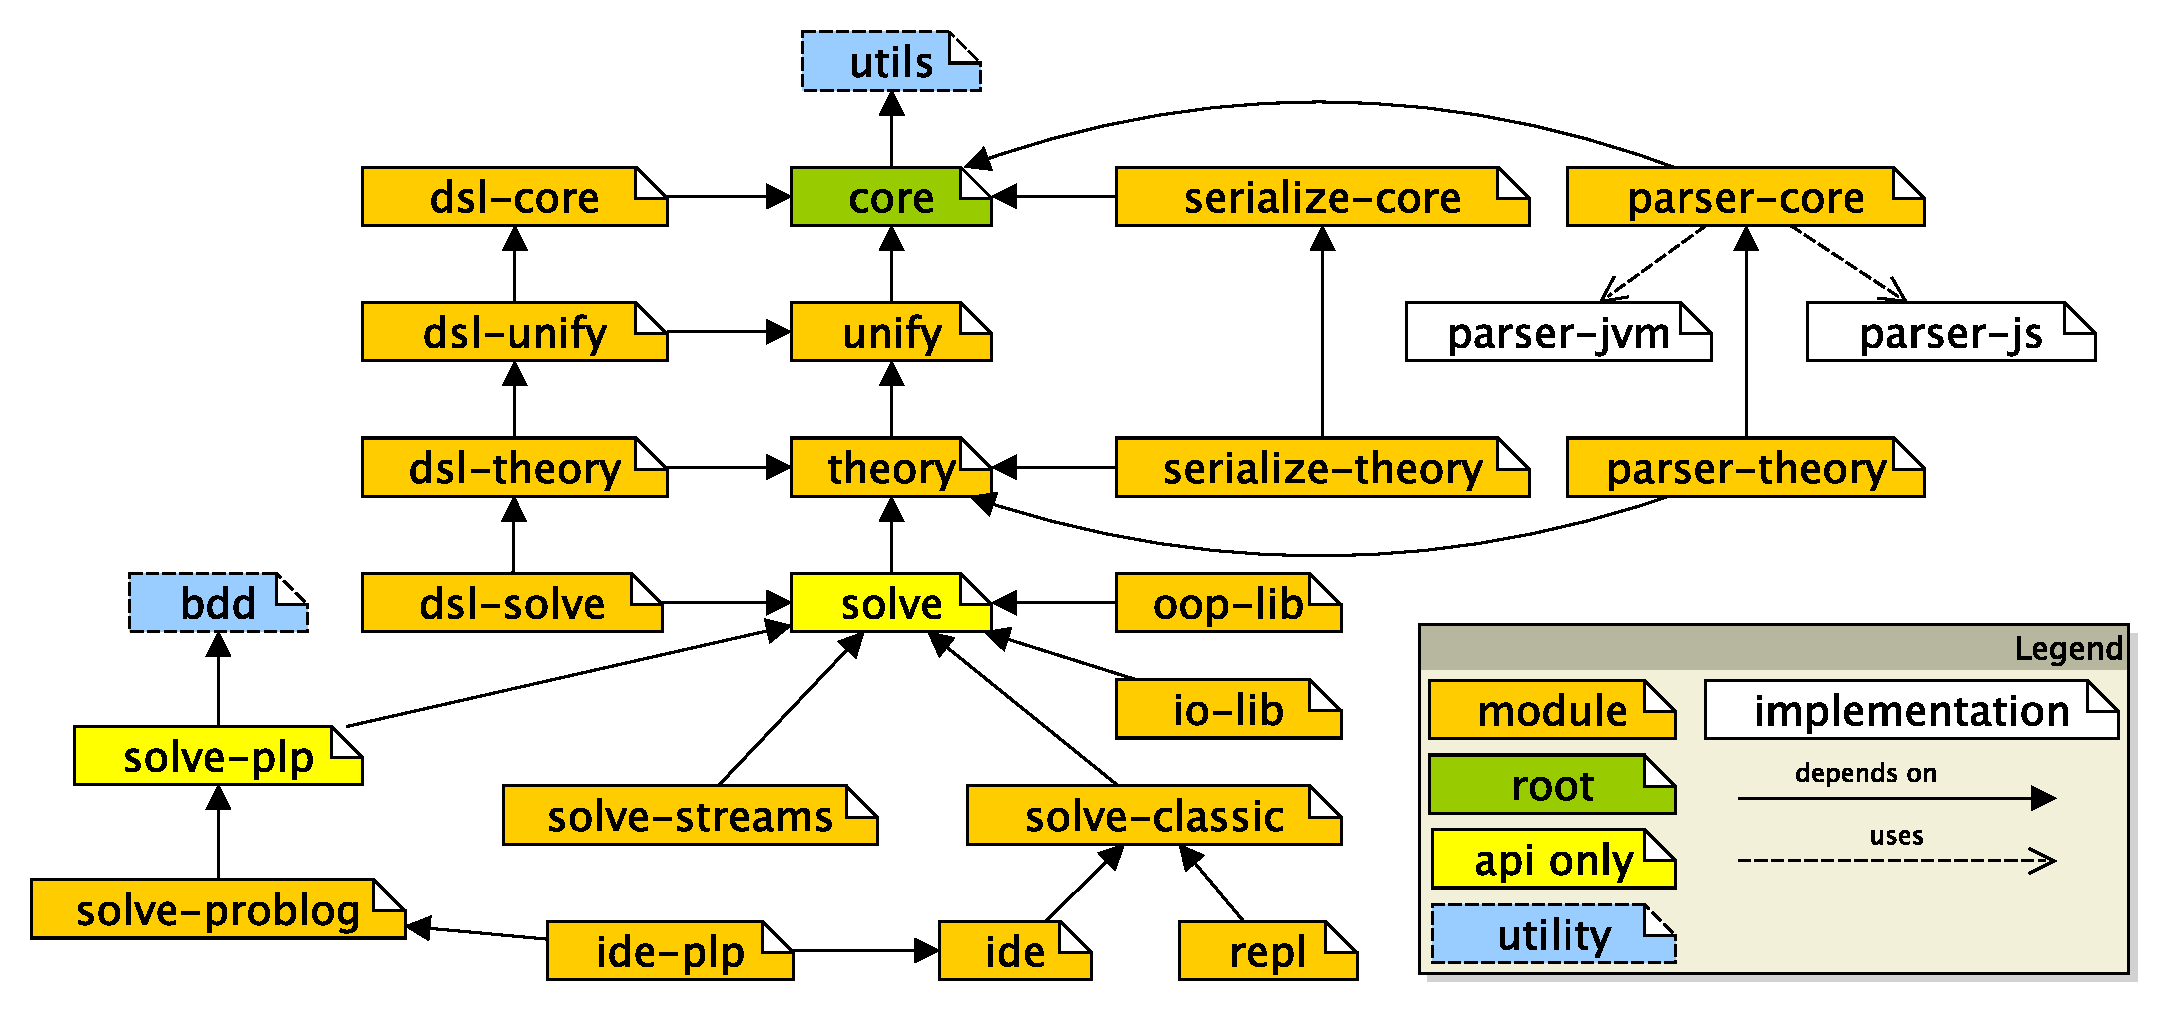
\includegraphics[width=\linewidth]{figures/2p-kt-project-map.pdf}
    \caption[\twopkt{} project map]{\twopkt{} project map: LP functionalities are partitioned into some loosely-coupled and incrementally-dependent modules}
    \label{fig:2p-kt-project-map}
\end{figure}

\twopkt{} is deeply rooted in CL, a programming paradigm based on computational logic \cite{lloyd1990computational,Nerode1996}.
%
Hence, from an architectural perspective, \twopkt{} is a framework supporting the creation of logic-based software via several loosely-coupled \emph{modules}---each one tailored on a particular aspect of CL.

To further support reusability, each module factorises a small number of related functionalities, via a compact API composed by OOP types and methods.
%
As modules are the most basic deployable units in \twopkt{}, major LP functionalities are partitioned into modules on a per-usage basis, to make them selectively usable as dependencies in other projects.
%
The \twopkt{} ecosystem itself is attained by incrementally combining such modules, as depicted in \cref{fig:2p-kt-project-map}.
%
Accordingly, to maximise interoperability, \twopkt{} modules are individually available as pre-compiled libraries both on Maven Central Repository (MCR)\footnote{\url{https://search.maven.org/search?q=g:it.unibo.tuprolog}} -- for JVM-, Android- or Kotlin-based contexts -- and on the NPM Registry\footnote{\url{https://www.npmjs.com/org/tuprolog}} -- for JS-based contexts --, whereas a detailed description of their API is available on the Web as part of \twopkt{} documentation.
%
% In the latter case, self-executing Jars for \twopkt{} GUI and CLI are available on the GitHub Release page\footnote{\url{\twopktRelease}} of the project, while a Web-based GUI is available at \cite{2P-Playground} for direct in-browser usage in a serverless fashion.

\begin{figure}
    \centering
    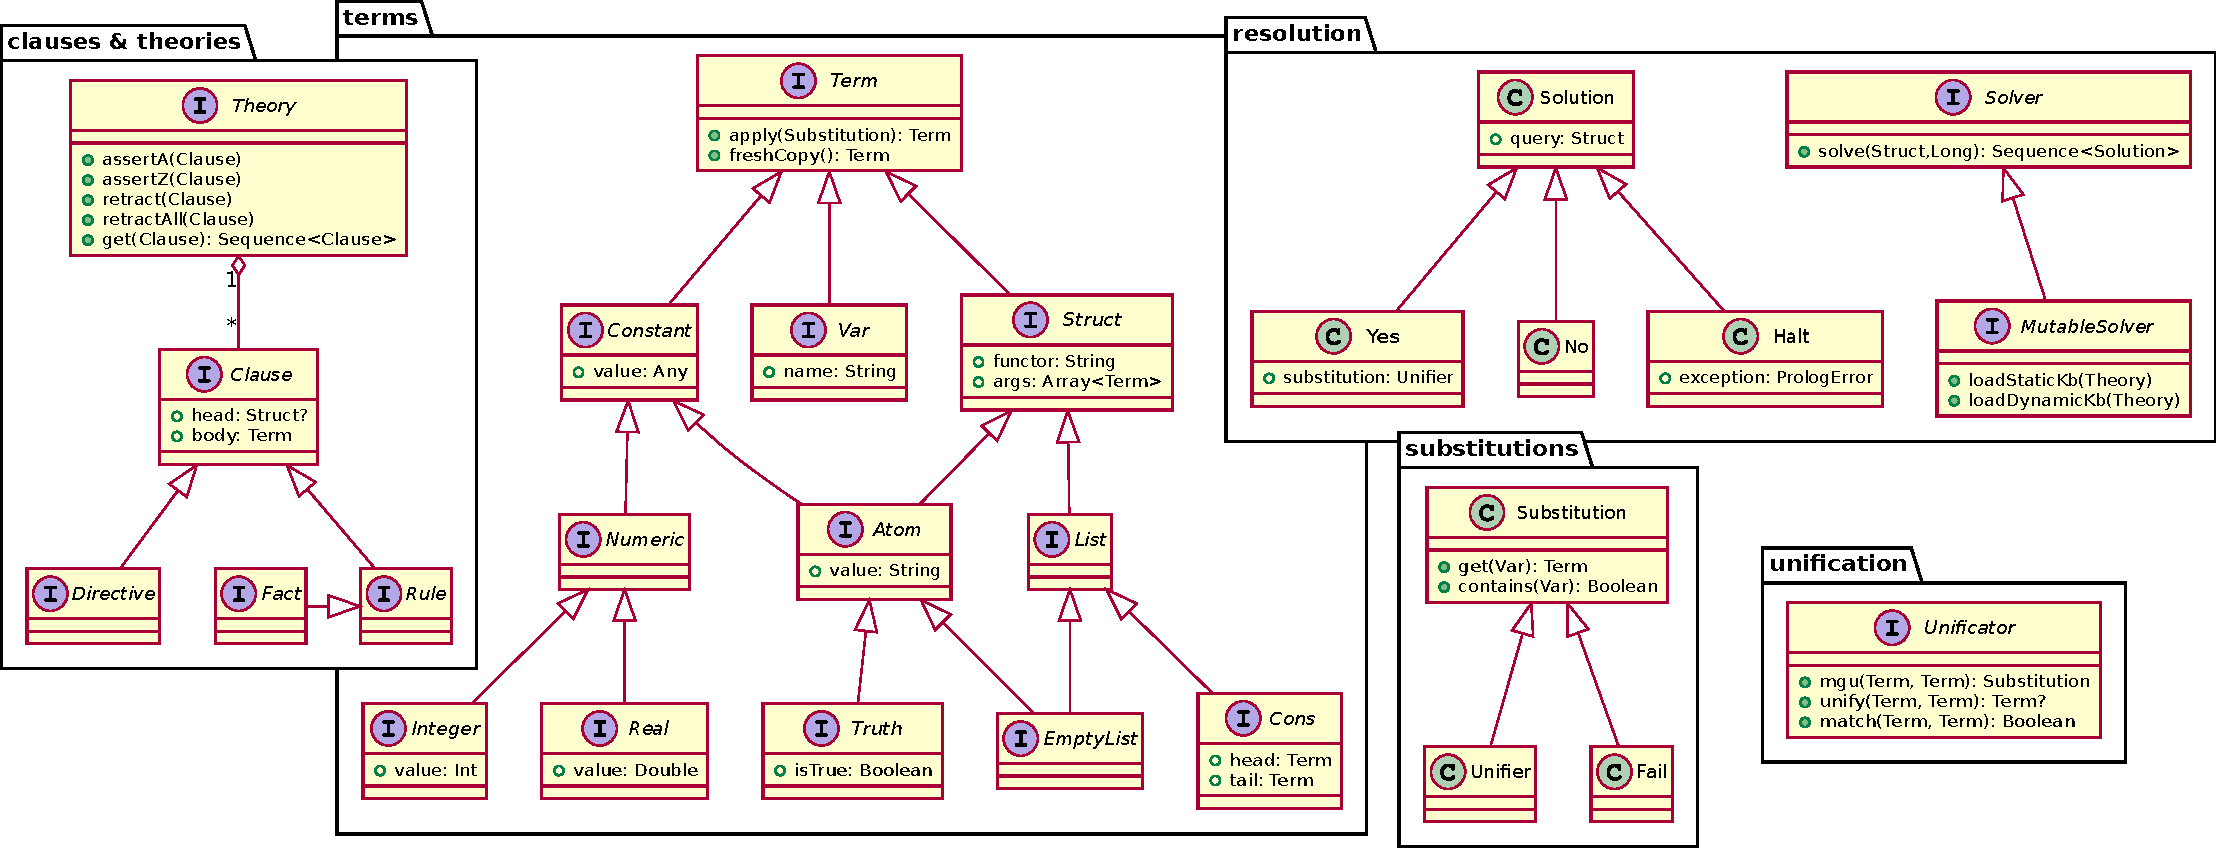
\includegraphics[width=\linewidth]{figures/2p-kt-api.pdf}
    \caption[\twopkt{} public API]{\twopkt{} public API: a type is provided for each relevant concept in LP}
    \label{fig:2p-kt-api}
\end{figure}

If all \twopkt{} modules were merged together, the most relevant aspects of their API could be summarised as in \cref{fig:2p-kt-api}.
% depicts the main aspects of \twopkt{} public API.
%
The diagram points out how all relevant aspect of LP are reified into types: e.g.
%
\begin{itemize}
    \item logic \texttt{Term}s (as well as any specific sort of term, e.g. \texttt{Var}iables, or \texttt{Struct}ures, etc.),
    \item logic \texttt{Substitution}s, unification, and MGU (computed by an \texttt{Unificator}),
    \item \texttt{Clause}s (there including \texttt{Rule}s, \texttt{Fact}s, and \texttt{Directive}s),
    \item knowledge bases and logic theories (e.g. the \texttt{Theory} type),
    \item automatic reasoning, via the \texttt{Solver} interface, and
    \item logic \texttt{Solution}s---computed by \texttt{Solver}s in response to queries.
\end{itemize}
%
There, interfaces are used to expose relevant aspects, in order to keep the system extensible.
%
Developers may e.g.\ define custom implementations for \texttt{Unificator} and \texttt{Solver} to provide novel inference mechanisms involving some variant of the unification algorithm.
%
Of course, a detailed diagram would include several more types, as the \twopkt{} API also supports:
%
\begin{inlinelist}
    \item (de)se\-ria\-li\-sa\-tion of logic terms and theories into/from standard data-representation formats such as JSON, or YAML;
    \item parsing/formatting logic terms and theories from/into concrete logic syntaxes such as Prolog's one;
    \item letting developers extend solvers via libraries of custom LP functionalities;
    \item letting users exploit logic solvers either by a command-line (CLI) and graphical (GUI) user interface;
\end{inlinelist}
%
etc.

\subsection{Overview of Functionalities}
\label{ssec:functionalities}

% Present the major functionalities of the software.

Each major \twopkt{} functionality is reified into a particular module.
%
Accordingly, in this subsection we enumerate \twopkt{} functionalities on a per-module basis.
%
Following Gradle convention, we denote modules by \module{mo\-du\-le\-Na\-me}.

The most fundamental module is \module{core}, which exposes types for representing symbolic knowledge via terms and clauses, other than methods to support their manipulation (e.g. construction, unfolding, scoping, formatting, etc.) for OOP or FP programmers.
%
It comes with several data structures aimed at covering most common KR needs in LP.
%
However, novel sorts of terms and clauses may optionally be added by developers by extending/implementing any public interface in \module{core}.
%
Furthermore, the pervasive adoption of an \emph{immutable} design makes data structures in \module{core} well suited for concurrent and multi-threaded contexts.

Terms and clauses are often compared or manipulated in LP via \emph{unification}.
%
Arguably \cite{Sterling1996}, unification \cite{unification-automatedreasoningbook2001} is -- by itself --, among the most useful contributions of LP to AI.
%
For this reason, we encapsulate it within an \emph{ad-hoc} module, \module{unify}, coming with a general notion of \texttt{Unificator} -- i.e. any algorithm aimed at computing MGU out of terms or clauses --, and a default implementation based on \cite{MartelliMontanari1982}.
%
Developers may extend the default implementation by configuring e.g. when terms should be considered equal or not, or they can provide a different implementation for \texttt{Unificator}, in case they need a specific unification strategy, or, they  prefer to adopt a different unification algorithm.

Another common need in LP is the in-memory storage of clauses into ordered -- e.g. queues -- or unordered -- e.g. multisets -- data structures, and their efficient retrieval via pattern-matching (e.g. unification).
%
The \module{theory} module follows this purpose, by providing notions such as \texttt{ClauseQueue}, \texttt{ClauseMultiset}---all coming both in an \emph{immutable} (access-efficient) and \emph{mutable} (update-efficient) implementation.
%
These data structures differ from ordinary collections as they enable a unification-based retrieval and indexing of clauses.
%
Prolog's notions of theory, and static/dynamic KB are built on top these data structures, exploiting the most adequate implementation in each case.

The practice of LP may also involve several ancillary operations over terms and clauses, e.g.:
%
\begin{inlinelist}
    \item formatting -- into some \emph{customisable} form --,
    \item (de)serialisation -- into/from open data-representation formats such as JSON or YAML --, and
    \item parsing---out of a particular concrete syntax, such as, e.g., Prolog syntax.
\end{inlinelist}
%
While formatting is considered a \module{core} functionality, attained via the \texttt{TermFormatter} type, (de)serialisation and parsing come with their own modules.
%
Thus, module \module{serialize-core} (resp. \moduleStyle{-theory}) supports the serialisation and deserialisation of terms (resp. theories) into JSON or YAML, according to a human-readable schema.
%
This is aimed at supporting distributed applications needing to exchange logic knowledge over the network.
%
Similarly, parsing terms (resp. theories) in Prolog syntax is currently supported through the \module{parser-core} (resp. \moduleStyle{-theory}) module, which is based on the well-known ANTLR technology \cite{Parr2013} for language engineering.

A generic API for logic solvers is available as well within the \module{solve} module.
%
Conceptually, the purpose of this module is as simple as exposing the \texttt{Solver} type, which represents any entity capable of performing some sort of logic resolution to provide one or more \texttt{Solution}s to a logic query.
%
However, resolution involves many practical aspects -- such as errors management, extensibility via libraries, I/O, etc. -- which are \emph{orthogonal} w.r.t. any particular resolution strategy.
%
This is why \module{solve} is a quite articulated -- despite not directly usable -- module.

While developers may easily build their inference procedure of choice by providing an implementation for the \texttt{Solver} interface -- possibly selectively reusing features from \module{solve} --, two implementations are currently available as part of \twopkt{} -- namely \module{solve-classic} and \moduleStyle{-streams} --, both implementing Prolog's SLDNF resolution strategy.
%
In particular, \module{solve-classic} is based on the work of Piancastelli et al. \cite{tuprolog-sac08} and is currently stable, while \module{solve-streams} is an experimental attempt of implementing Prolog via LP following the idea proposed in \cite{Carlsson84}.
%
Notably, none of them relies on the Warren Abstract Machine \cite{Warren1983}---the computational model Prolog is commonly built upon.

A generic API for developing Prolog-like predicates in Kotlin is available as well.
%
It heavily leverages FP and OOP to let developers extend their solvers with libraries of complex functionalities -- possibly involving backtracking or side-effects -- which are easier to implement in Kotlin than through LP.
%
There, lazy streams of data are treated as flows of solutions to be enumerated via backtracking.
%
This makes \twopkt{} very well-suited for handling possibly infinite streams of data via LP -- an essential feature in modern AI -- as further discussed in \cref{chap:lp-streams}.

User experience (UX) is enabled by two more modules -- namely, \module{repl} and \module{ide} --, which provide a CLI and GUI, respectively.
%
While they both target JVM-specific UX, an experimental web-based GUI is available at \cite{2P-Playground}, targetting JS-specific UX.

The many \module{dsl-*} modules in \cref{fig:2p-kt-project-map} are aimed at supporting the Kotlin-based DSL for LP described in \cite{kotlindsi4prolog-woa2020}.
%
It consists of façade to \twopkt{} API aimed at blending the OOP, FP, and LP programming paradigms via Kotlin's flexible syntax.
%
Within the \twopkt{} project, this DSL is extensively exploited for unit testing.

Finally, the \module{oop-lib} module is experimental logic library aimed at supporting the exploitation of OOP from within logic programs.

\section{Illustrative Examples}
\label{sec:illustrations}

% Provide at least one illustrative example to demonstrate the major functions.

% Optional: you may include one explanatory video that will appear next to your article, in the right-hand side panel. (Please upload any video as a single supplementary file with your article. Only one MP4 formatted, with 50MB maximum size, video is possible per article. Recommended video dimensions are 640 x 480 at a maximum of 30 frames/second. Prior to submission please test and validate your .mp4 file at $ http://elsevier-apps.sciverse.com/GadgetVideoPodcastPlayerWeb/verification$. This tool will display your video exactly in the same way as it will appear on ScienceDirect.).

\begin{figure}\centering
    \begin{subfigure}{.49\linewidth}
        \includegraphics[width=\linewidth]{figures/2p-ide-all.png}
        \caption{The \twopkt{} GUI}
        \label{fig:gui}
    \end{subfigure}
    %
    \hfill
    %
    \begin{subfigure}{.49\linewidth}
        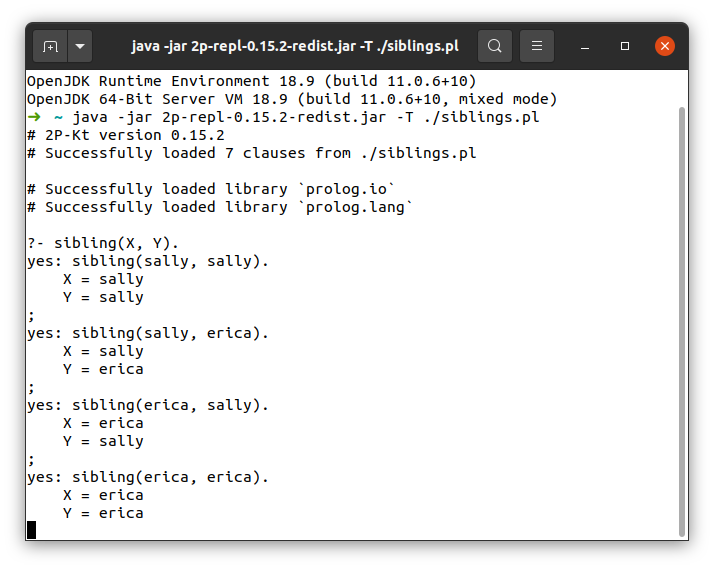
\includegraphics[width=\linewidth]{figures/2p-kt-repl.png}
        \caption{The \twopkt{} CLI}
        \label{fig:cli}
    \end{subfigure}

    \begin{subfigure}{.49\linewidth}
        \includegraphics[width=\linewidth]{figures/2p-playground.png}
        \caption{The \twopkt{} Playground \cite{2P-Playground}}
        \label{fig:playground}
    \end{subfigure}
    %
    \hfill
    %
    \begin{subfigure}{.49\linewidth}
        \includegraphics[width=\linewidth]{figures/2p-kt-dsl.png}
        \caption{Usage of the Kotlin DSL for Prolog \cite{kotlindsi4prolog-woa2020}, within an IDE}
        \label{fig:dsl}
    \end{subfigure}
    \caption{Usage examples for \twopkt{}}
    \label{fig:usage-examples}
\end{figure}

% \cref{fig:usage-examples} shows the many possible usages \twopkt{}.
%
% More precisely, \cref{fig:gui} depicts its GUI for Prolog, whereas \cref{fig:cli} depicts its CLI.
% %
% Similarly, \cref{fig:playground} depicts the web GUI \cite{2P-Playground} of \twopkt{}, running within the Chrome Browser and only relying on the generated JS code.
% %
% Finally, \cref{fig:dsl} depicts the usage of \twopkt{}'s DSL for Prolog within a simple Kotlin script running within the IntelliJ Idea IDE.

% \gcnote{Espandiamo la discussione o mettiamo solo gli screenshot? Nel primo caso, cosa dico per ogni screenshot?}

The \twopkt{} GUI (\cref{fig:gui}) consists of a minimal IDE based on Java FX.
%
It supports users willing to exploit LP interactively, possibly editing a theory repeatedly, performing different queries, and inspecting the mutable internals of the underlying solver.
%
Accordingly, the GUI lets users open several files at once, perform queries one-by-one or all-at-once, or inspect the currently loaded libraries, operators, flags, etc.
%
Syntax colouring completes the picture, easing users' writing of logic theories.

% \begin{figure}\centering
    %     \includegraphics[width=.7\linewidth]{img/2p-ide-all.png}
    %     \caption{The \twopkt{} GUI}
    %     \label{fig:gui}
    % \end{figure}

Conversely, the \twopkt{} CLI (\cref{fig:cli}) lets users issue their queries against logic solvers via a textual console.
%
It supports both an interactive and non-interactive operation mode.
%
In the former case, the application consists of a Read-Eval-Print-Loop accepting logic queries from \texttt{stdin} and progressively prompting solutions to \texttt{stdout}.
%
In the latter case, queries and theories are provided as arguments upon CLI launch and the program terminates after prompting all possible solutions.

% \begin{figure}\centering
    %     \includegraphics[width=.7\linewidth]{img/2p-repl-light.png}
    %     \caption{The \twopkt{} CLI}
    %     \label{fig:cli}
    % \end{figure}

The \twopkt{} Playground (\cref{fig:playground}) is currently a proof-of-concept web application which only lets users write/load theories, issue logic queries, and visualise the corresponding solutions in their browsers.
%
% Its main purpose is to demonstrate how the generated JS sources can actually be exploited  within browser- and server-side JS projects.
%
The key point here is that a full-fledged \twopkt{} application can be executed in-browser in a server-less fashion.
%
In fact, our Playground only requires Internet connection upon page loading.
%
After that, it does not interact with the server any longer as the loaded JS scripts are more than sufficient to make \twopkt{} usable from within users' browsers.
%
For this reason, logic computations performed through our Playground need not any sandbox -- as no server is needing to be protected against DoS attacks --, nor logic solvers need API limitation for security reasons.

% \begin{figure}\centering
    %     \includegraphics[width=.7\linewidth]{img/2p-playground.png}
    %     \caption{The \twopkt{} Playground \cite{2P-Playground}}
    %     \label{fig:playground}
    % \end{figure}

Finally, \twopkt{}'s DSL for Prolog can be exploited within Kotlin projects as shown in \cref{fig:dsl}.
%
Essentially, it provides a syntactical way to inject LP into Kotlin scripts.
%
To make this possible, users must import one or more \module{dsl-*} module as dependencies into their Kotlin projects, e.g. via Gradle or any other build system.
%
As discussed in \cite{kotlindsi4prolog-woa2020}, the adoption of this DSL makes the life of logic programmers easier, as they can automatically inherit the many tools available for Kotlin development---e.g. type checking, linters, code completion, debugging, etc.

% \begin{figure}\centering
    %     \includegraphics[width=.7\linewidth]{img/2p-kt-dsl.png}
    %     \caption{Usage of the Kotlin DSL for Prolog \cite{kotlindsi4prolog-woa2020}, within an IDE}
    %     \label{fig:dsl}
    % \end{figure}

\section{Impact}
\label{sec:impact}

We expect \twopkt{} technology to have an impact on many research areas.

Within the scope of LP, for instance, \twopkt{} provides a well-grounded technological basis for implementing (or building variants and extensions of) the many solutions proposed into the literature---there including abductive inference procedures \cite{FungIff97}, rule induction methods \cite{Muggleton94}, probabilistic reasoning \cite{RaedtK15}, labelled LP \cite{labelledlp-fi161}, etc.)

Furthermore, as recently shown in \cite{lptech4mas-jaamas35}, the multi-agent systems community have quite an appetite for  \emph{interoperable} and general-purpose logic-based technologies.
%
There, \twopkt{} may provide a technological substrate supporting agent automated reasoning via manifold reasoning mechanisms.

Similarly, \twopkt{} represents a valuable technological choice within the field of Coordination \cite{MaloneC94}.
%
As demonstrated in \cite{coordination-jlamp2020}, many tuple-based coordination models and technologies rely on LP and logic-based technologies at the fundamental level.
%
There, \twopkt{} enables the implementation of \emph{interoperable} \linda{} tuple spaces -- such as in \tusow{} \cite{tusow-icccn2019} -- or tuple \emph{centres}---as we plan to do in \tucson{} \cite{tucson-jaamas2}.

Moreover, as discussed in \cite{kotlindsi4prolog-woa2020}, \twopkt{} impacts on programming paradigms as well.
%
In fact, while most successful programming paradigms (imperative programming, OOP, FP) are being increasingly \emph{blended} into modern programming languages, LP remains somewhat isolated.
%
In this context, \twopkt{}'s DSL for LP paves the way towards the integration of LP with other programming paradigms.

Finally, we expect \twopkt{} will have a role to play in the field of explainable AI.
%
There, the integration among symbolic and sub-symbolic AI is considered a strategical research direction \cite{xaisurvey-ia14} and \twopkt{} may offer a sound technological basis to this purpose.

\paragraph{\twopkt{} adoption}

While \tuprolog{} has been exploited both in the industry and in the academia\footnote{\url{http://apice.unibo.it/xwiki/bin/view/Tuprolog/Users}}, \twopkt{} has been used in the academia only---so far.
%
However, it has already worked -- or, will work in the near future -- as the technological basis of many scientific contributions.
%
Some, such as \tucson{} \cite{tucson-jaamas2}, \respect{} \cite{respect-scp41}, \lpaas{} \cite{lpaas-bdcc2}, or \tenderfone{} \cite{blockchainmas-applsci10} leveraged on \tuprolog{} for their implementation, and are now being migrated on \twopkt{}.
%
Others, such as \tusow{} \cite{tusow-icccn2019}, \argtwop{} \cite{arg2p-cilc2020}, or the Kotlin-based DSL for LP proposed in \cite{kotlindsi4prolog-woa2020} are already based on \twopkt{}.

% Indicate in what way, and to what extent, the pursuit of existing research questions is improved (if so).
\paragraph{Research directions stemming from \twopkt{}}

Currently, \twopkt{} is already enabling the exploration of many interesting research questions thanks to its modularity and interoperability.
%
Any research line involving symbolic manipulation or automated reasoning is then likely to benefit from \twopkt{} functionalities.
%
Generally speaking, \twopkt{} paves the way towards:
%
%\begin{inlinelist}
%    \item
    the coexistence and integration of different LP aspects,
%    \item
    the hybridisation of LP with other AI techniques, and
%    \item
    the exploitation of LP in building flexible intelligent systems.
%\end{inlinelist}
%
Along these lines, our goals involve:
%
\begin{inlinelist}
    \item\label{goal:multi-logic} the creation of comprehensive solvers capable of exploiting multiple inference procedures, knowledge-representation means, etc. at once in answering users' queries,
    \item\label{goal:hybrid-lp} the construction of hybrid systems where logic programmers can transparently exploit machine learning (ML) and sub-symbolic AI, and
    \item\label{goal:lp-and-mas} the injection of LP into cognitive agents architectures.
\end{inlinelist}

So, as far as goal \ref{goal:multi-logic} is concerned, we are currently exploring the design of probabilistic, abductive, or concurrent resolution under a unique API.
%
These functionalities may constitute novel modules enriching the \twopkt{} ecosystem.
%
This would enable further research towards, e.g., \emph{mixed} reasoning processes, where multiple inference procedures can be dynamically interleaved while answering some user's query.

As far as goal \ref{goal:hybrid-lp} is concerned, we are currently exploring the design of a logic-based API for ML and, in particular, neural networks.
%
The API allows logic-programmers to define, train, assess, and use sub-symbolic predictors via LP.
%
At the technical level, the API are reified into yet another module enriching the \twopkt{} ecosystem.
%
This would enable further research towards, e.g., the integration of symbolic and sub-symbolic AI, the automation of ML workflows, and the exploitation of fuzzy knowledge induced from data in LP.

Finally, as far as goal \ref{goal:lp-and-mas} is concerned, we are currently exploring the integration of multiple logics within BDI architectures.
%
The idea here is to enable intelligent agents to perform the most adequate sort of reasoning or knowledge-representation means for the situation at hand.
%
This would enable further research towards, e.g., the exploitation of different logics (e.g. first-order, temporal, spatial, deontic, etc.) to support intelligent, context-specific behaviour for software agents.
%
There, \twopkt{} provides a common ground for the implementation of automated reasoners supporting each logic.

\emptyparagraph

Accordingly, in the reminder of this thesis, we explore a number of contributions stemming from (and enabled by) \twopkt{}.

In particular, in \cref{chap:lp-streams}, we introduce a fundamental mechanism -- namely, \emph{primitives} -- which \twopkt{} solvers may exploit to lazily handle streams of data.
%
Despite its simplicity, the mechanism is very powerful, as it enables the interoperability of LP with other runtimes, e.g. JVM libraries.
%
This, in turn, enables most of the subsequent contributions discussed in this thesis.
%
Similarly, in \cref{chap:kt-dsl}, we discuss the integration of logic, object-oriented, and functional programming at the paradigm and language level, as made possible by \twopkt{}.

In \cref{chap:mllib}, we propose the design of a logic API for ML, aimed at enabling the manipulation of ML predictors in LP, and, therefore, the creation of hybrid (symbolic + sub-symbolic) AI solution.
%
We also discuss how such API can be reified into yet another module expanding the \twopkt{} ecosystem.

In \cref{chap:psyke}, we propose the design and implementation of a ``platform for symbolic knowledge extraction'' (\psyke{}) reifying the vision and the architecture discussed in \cref{sec:knowledge-extraction}.
%
The proposed technology enables the extraction of logic rules out of sub-symbolic predictors.
%
Such rules are of course represented as clauses, as enabled by \twopkt{}.

Furthermore, in \cref{chap:plp} we discuss the extension of the \twopkt{} ecosystem towards probabilistic logic programming.
%
Despite the benefits of supporting probabilistic reasoning, such extension confirms the advantages of the ecosystem-based approach.
%
In fact, we show how probabilistic reasoning support can be achieved by reusing as much functionalities from the \twopkt{} ecosystem as possible.

Finally, in \cref{chap:2pkt-future} we discuss a number of future research directions, stemming from or overlapping \twopkt{}.
%
Despite some steps have already been performed along these directions, they are not mature enough to be included as chapters in this thesis.
%
Hence, we report them as future works, providing insights about their backgrounds and presenting what we have already done so far.


%\section{Summarising}
%\label{sec:conclusion}
%
%This chapter introduces \twopkt{}, an open, general, Kotlin Multiplatform ecosystem for LP, supporting manifold mechanisms for automated reasoning, via several loosely-coupled modules.
%%
%Each module makes some specific LP aspects individually usable.
%%
%Selectively reusing/extending modules enables bootstrapping novel LBT without re-implementing everything from scratch or producing Prolog-centered monoliths.
%%
%In particular, \twopkt{} supports \emph{mixed} inference procedures, involving both symbolic and sub-symbolic techniques.
%
%The \twopkt{} ecosystem is structured by keeping reusability, extensibility and interoperability in mind.
%%
%Its functionalities include knowledge representation, (de)serialisation, parsing (and formatting facilities), unification,
%clause in-memory indexing and storage facilities, logic inference via SLDNF, UX, and rich Kotlin API for developers.
%%
%They all support JVM, JavaScript, and Android platforms.
%
%\note{Whet the appetite of the reader by spoilering next chapters}

\chapter{Bridging LP and Stream Processing}
\label{chap:lp-streams}

\mypapers{2pkt-jelia2021}

Streams are a powerful abstraction in computer science as they enable the processing of huge amounts of data, especially when keeping all data in memory would be impractical or infeasible.
%
In the era of the Internet of Things (IoT) and data-driven artificial intelligence (AI), the ability of manipulating possibly unlimited streams of data is a must-have for all programming paradigms and languages.
%
Indeed, a growing amount of application scenarios are characterised by the pervasive exploitation of smart devices generating/capturing huge amounts of data, as well as of the software infrastructures aimed at processing them.

A stream is an \emph{ordered sequence} of data that may or may not be limited in length.
%
Stream processing facilities are thus commonly constructed in such a way that streams are \emph{lazily consumed}, in order to minimise the amount of required memory---which may be soon saturated otherwise.
%
However, despite all sorts of streams are lazily consumed, categories may be drawn depending on how they are \emph{generated}.
%
Depending on how the are \emph{generated}, streams are either \emph{cold} (a.k.a.\ \emph{pull}) or \emph{hot} (a.k.a.\ \emph{push}).
%
Each item of a cold stream is generated on the fly, as soon as a consumer \emph{pulls} it from the stream.
%
In the case of hot streams, instead, an external entity is supposed to be in charge of generating items and \emph{pushing} them to the stream, so that consumers can retrieve them in a FIFO way.

Cold streams are the simplest ones.
%
A cold stream can be naturally attained via functional programming and higher-order functions (e.g. \texttt{map}, \texttt{filter}, \texttt{reduce}): this is why mainstream programming languages such as Java, C\#, Python, JavaScript, Scala, Kotlin, etc., are being extended to blend functional features and constructs for dealing with streams.
%
Conversely, hot streams are more complex, as they require data to be buffered while waiting for consumption---making them ideal for \emph{temporally} decoupling data consumers and producers.
%
In particular, hot streams are key enablers of advanced stream processing techniques, such as sliding windows, or complex event processing (CEP)---which are deeply entangled with the \emph{time}-related aspects of data production.

In this scenario,  logic programming (LP), as well, has its role to play, both in data-driven AI -- in particular in relation to explainable systems \cite{xaisurvey-ia14} -- or in the IoT \cite{lpaas-bdcc2}.
%
For instance,  LP and rule-based frameworks are generally recognised as well-suited to support CEP~\cite{AnicicFRSSS10,AnicicRFS12}, as they are expressive enough to capture complex events from hot streams.
%
Similarly, answer-set programming (ASP) has been extensively exploited as a means for reasoning over hot streams of data~\cite{EiterIST05,BeckEB17,Beck2018}.

In this chapter, we focus on the Prolog~\cite{ColmerauerR93} programming language---arguably, the most popular LP language.
%
Currently, Prolog can hardly be considered as a suitable stream-processing technology~\cite{Tarau2019}, as it provides minimal support for consuming both cold and hot streams.
%
However, we believe that this should be reconsidered because Prolog already supports the lazy exploration of possibly infinite search spaces via \emph{backtracking}.
%
Thus, the problem with Prolog is not to discuss \emph{whether} it supports stream processing or not, but rather \emph{how}.

Existing solutions extend Prolog with syntactical, semantical, or library enhancements aimed at supporting cold streams explicitly.
%
Conversely, in this chapter, we discuss how Prolog can be reinterpreted as a \emph{stream processing tool}, capable of manipulating both cold and hot streams of data.
%
In particular, our solution does not affect the syntax (nor the operation) of the Prolog language.
%
More precisely, we show how Prolog predicates may be interpreted as \emph{primitives} of streams to be lazily consumed via backtracking.
%
Along this line, we present an abstract design for Prolog solvers based on finite-state machines, aimed at supporting our notion of primitives.
%
Finally, a practical demonstration based on the \twopkt{} technology \cite{homepage2PKt} is discussed showing how primitives may let a Prolog solver consume events from the external world in a transparent way.


%%%%%%%%%%%%%%%%%%%%%%%%%%%%
\section{Logic Solvers as Streams Prosumers}\label{sec:primitives}
%%%%%%%%%%%%%%%%%%%%%%%%%%%%

\subsection{Logic solvers as stream producers}

\begin{figure}
    \centering
    \caption{Interaction modes between logic solvers and users or KB}
    \label{fig:user-solver-interaction}
    \begin{subfigure}{0.48\linewidth}\centering
        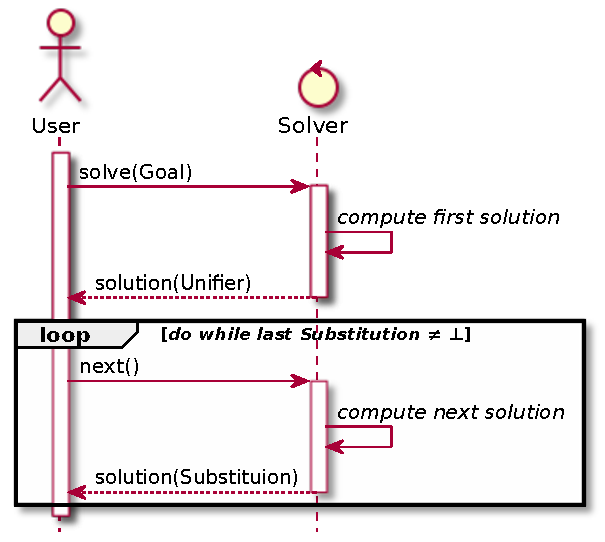
\includegraphics[width=\linewidth]{figures/stateful-solver.pdf}
        \caption{In \emph{stateful interaction} mode, solvers expose two functionalities: \texttt{solve} -- to compute the first solution to some query --, and \texttt{next}---to compute subsequent solutions to the same query}
        \label{fig:user-solver-interaction:stateful}
    \end{subfigure}
    \hfill
    \begin{subfigure}{0.48\linewidth}\centering
        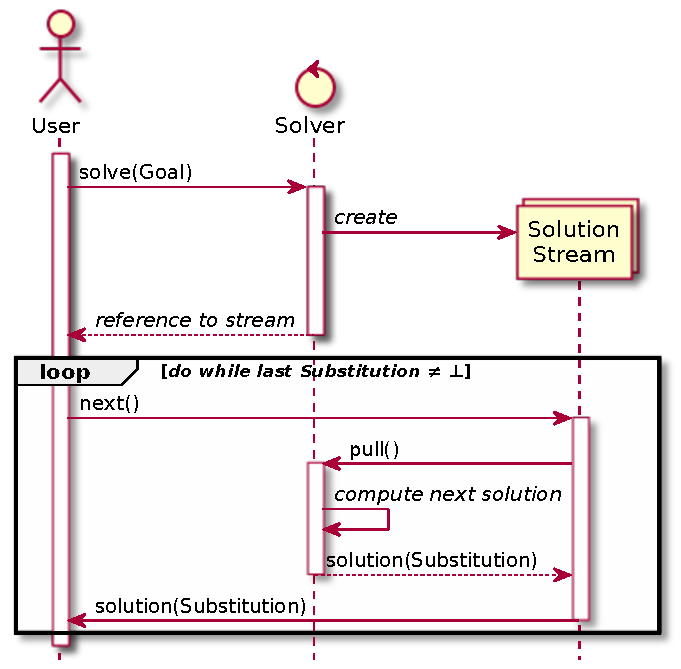
\includegraphics[width=\linewidth]{figures/streamful-solver.pdf}
        \caption{In \emph{stream-oriented interaction} mode, solvers expose one functionality: \texttt{solve}---which simply returns a stream of solutions that users may lazily consume}
        \label{fig:user-solver-interaction:streams}
    \end{subfigure}

    \begin{subfigure}{0.48\linewidth}\centering
        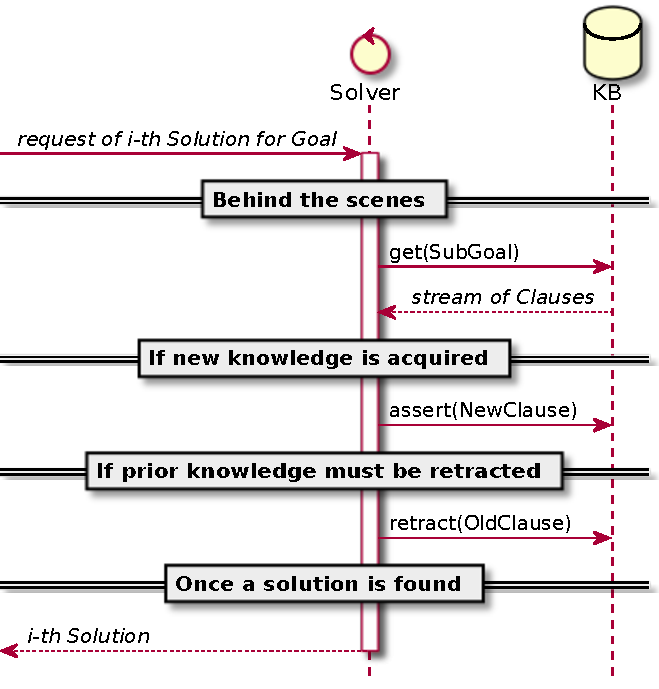
\includegraphics[width=\linewidth]{figures/streamful-kb.pdf}
        \caption{Interaction among a logic solver and its KB. As possibly mutable containers of knowledge KB expose three main functionalities: \texttt{get($C$)} returns a \emph{stream} of clauses matching $C$ via unification, whereas \texttt{assert($C$)} (resp. \texttt{retract($C$)}) adds (resp. removes) some clause (unifying with) $C$}
        \label{fig:solver-kb-interaction}
    \end{subfigure}
\end{figure}

Logic solvers \emph{à la Prolog} are typically queried \emph{interactively} by LP users in different \emph{modes}, which are naturally captured by the message passing perspective adopted in \cref{fig:user-solver-interaction}.
%
The most common mode of interaction among users and logic solvers is summarised in \cref{fig:user-solver-interaction:stateful}: users submit \emph{queries} (a.k.a.\ \emph{goals}) to a logic solver -- e.g. a Prolog interpreter -- via some \textit{ad-hoc} operation---e.g., \texttt{solve}.
%
Assuming that one or more \emph{solutions} exist, the solver computes and returns one of them---typically in terms of a \emph{unifying substitution}, assigning values to the query variables of interest for the user.
%
However, the user may be interested in solutions other than the first one: so, the solver should expose one further operation -- e.g., \texttt{next} -- letting users asking for further solutions to some previously-submitted query.
%
Finally, when no (more) solutions are available for a query, the solver can return one (last) answer carrying the \emph{failed} substitution (represented by $\bot$ in \cref{fig:user-solver-interaction}) instead of a unifier.

This mode of interaction is very effective since it enables the \emph{lazy} enumeration of a possibly infinite amount of solutions.
%
However, it comes with a few drawbacks.
%
First, despite logic solvers are actually capable of generating streams of solutions, the notion of stream is somewhat \emph{implicit} in the solver machinery---therefore, not explicitly exploitable.
%
Second, solvers are \emph{stateful}, in that they are responsible to keep track of the status of the interaction with each querying user.

To overcome these issues we suggest a shift of perspective, as depicted in \cref{fig:user-solver-interaction:streams}.
%
There, users and solvers interact in a \emph{stream-oriented} mode, where the stream of solutions is \emph{explicit} and the interaction between solvers and users is \emph{stateless}.
%
Thus, solvers expose just one operation -- i.e., \texttt{solve} -- accepting a user's query and returning a reference to the related \emph{cold} stream of solutions.
%
Users just need solvers to create solution streams that users can then lazily consume on demand.
%
Of course, solutions can still be produced lazily behind the scenes: whenever a user tries to consume a new solution, it can be computed on the fly.

Thus, even though interaction does not change from the operational viewpoint, our approach overcomes the limits of traditional logic solvers: solution streams here are \emph{explicitly} represented, and can therefore be \emph{manipulated} as such.

\subsection{Logic solvers as stream consumers}

By adopting a message passing perspective, logic solvers do not interact with users only.
%
Indeed, logic solvers typically act on a \emph{knowledge base} (KB).
%
In the general case, KBs are containers of the specific knowledge required by solvers to compute solutions to users' queries.
%
For instance, KB for Prolog solvers contain both rules and facts as Horn clauses, and are either static or dynamic.

From an interaction perspective, however, a KB is just a component exploited by solvers as part of their resolution process.
%
More precisely, solvers may need KB to retrieve some clauses, selected via unification, or, to retract or store some knowledge possibly learned/acquired during the resolution.

In particular, clause retrieval highlights how the interaction between solver and KB can be described in terms of streams as well.
%
As depicted in \cref{fig:solver-kb-interaction}, clause retrieval from KB can be modelled as an operation -- e.g., \texttt{get} -- accepting a clause template $C$ and returning the \emph{stream} of clauses unifying with $C$ currently stored into the KB.
%
The solver can then consume the stream as needed, e.g. either lazily or not, depending on the search strategy adopted.

Finally, storing a clause in the KB can be modelled as an \texttt{assert} accepting a clause $C$ and adding it to the KB, whereas clause retraction can be modelled as a \texttt{retract} accepting a clause template $C$ and removing a clause $C'$ unifying with $C$.
%
Both operations could be exploited either by the solver or by some \emph{external} entity willing to affect the solver's knowledge.

%%%%%
\subsection{Solvers vs. the World}

Yet, how can logic solvers deal with event streams coming from the external world?
%
Once KBs are recognised as individual entities, a trivial answer could be: \emph{via KB}.
%
External events may indeed be \emph{reified} into actual knowledge to be stored into some solver's KB.
%
In this scenario, external event streams should be translated into a sequence of \texttt{assert}ions aimed at injecting events into the KB, as facts.
%
The solver could then lazily consume the events by \texttt{get}ting or \texttt{retract}ing the corresponding facts from the KB.

There are, however, two major drawbacks in this approach.
%
First, the reification of events into KB requires space.
%
Second, solvers do not necessarily have to process or \emph{consume} reified events---thus a lot of space is wasted.
%
Accordingly, a different approach is required to let solvers consume event streams from the external world without reifying them unnecessarily.

In this work, we propose \emph{primitives} as the basic means to let solvers interact with the external world.
%
A primitive is a special Prolog facility capable of affecting and inspecting the external world via some I/O facility (\cref{fig:primitives}).
%
It is invoked by a solver and produces a \emph{stream of facts} to be consumed by the same solver.
%
However, from the solvers' perspective, primitives are ordinary built-in predicates denoted by \emph{signatures}---i.e., name/arity couples of the form $p/n$.

\begin{figure}\centering
    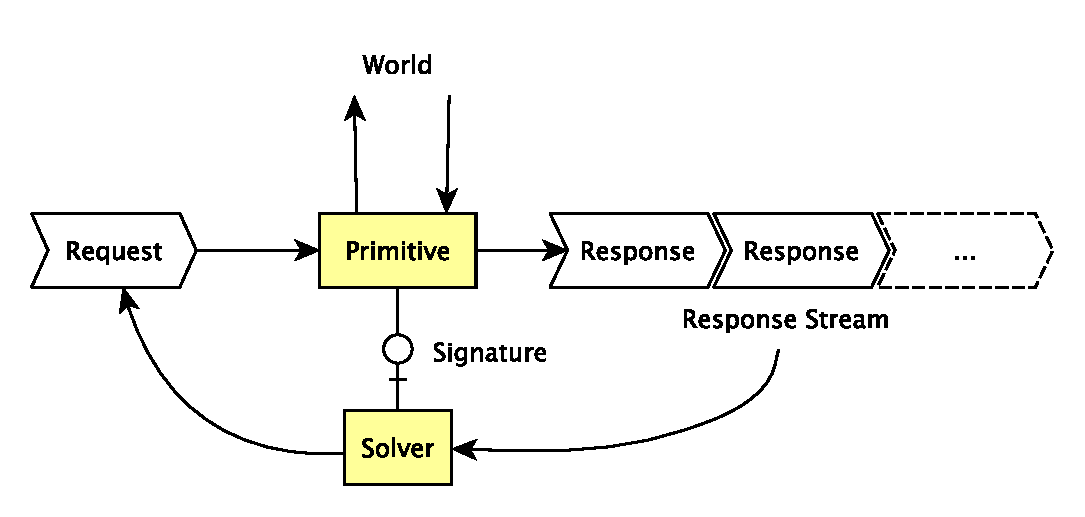
\includegraphics[width=\linewidth]{figures/primitive.pdf}
    \caption{Dataflow and component view of \emph{primitives}, i.e.\ solvers' gates towards the external world}
    \label{fig:primitives}
\end{figure}

More precisely, whenever the solver needs to compute the assignment of variables $T_i$ satisfying relation $p(T_1, \ldots, T_n)$, it can trigger the primitive denoted by $p/n$ (if it exists), by sending the $p/n$ primitive a \emph{request} providing a snapshot of the current resolution context and possibly an initial assignment of some $T_i$.
%
The primitive answers by providing a stream of \emph{responses} -- each one with some possible complete assignment of $T_i$ -- that the solver can consume accordingly to its resolution strategy---i.e., possibly later.
%
To produce responses, primitives may take into account several information sources -- e.g., the resolution context, the external world -- as a part of the request.
%
They may also attempt to \emph{affect} the external world via some I/O \emph{action}---e.g., triggering a sensor.

Depending on the numbers of responses a primitive provides, it can either be classified as either \emph{functional} or \emph{relational}.
%
Functional primitives produce just one response and their execution is therefore analogous to the execution of a function, as they consume an input and return a single result.
%
Conversely, relational primitives produce two or more responses.

%-----------------------------------------------------------------------------------------------%
\subsection{Example: TSP in Prolog}\label{ssec:tsp}
%-----------------------------------------------------------------------------------------------%

Let us consider for instance the case of a user exploiting a standard Prolog system to solve arbitrary instances of the Traveling Salesman Problem (TSP).

Let us assume the system requires maps to be represented as facts in the form \prolog{path(+Src, +Dst, +Cst)} -- each one representing an undirected path between two locations, and the estimated cost --, like e.g.:
%
\begin{lstlisting}[language=Prolog]
path(bucarest, giorgiu, 90).
path(bucarest, pitesti, 101).
path(pitesti, 'rimnicu vilcea', 97).
path(pitesti, craiova, 138).
path('rimnicu vilcea', craiova, 146).
...
\end{lstlisting}
%
Under this assumption, Prolog exposes a predicate \prolog{tsp(?Cities, ?Circuit, ?Cost)} aimed at computing the best \prolog{Circuit} for some set of \prolog{Cities}, and the corresponding \prolog{Cost}---where, \prolog{Cities} is a set of cities, \prolog{Circuit} is a list of cities to be visited in a row, and \prolog{Cost} is an integer.
%
Following a purely-logical interpretation, the predicate represents a ternary relation $\texttt{tsp} \subseteq 2^\mathcal{C} \times \mathcal{C}^* \times \mathbb{N}$ grouping subsets of cities, lists of cities, and non-negative integers, where $\mathcal{C}$ is the set of all cities mentioned in the KB as either the first or second argument of a \prolog{path/3} fact, and $\mathcal{C}^*$ is the Kleene-closure of $\mathcal{C}$.
%
Thus, an assignment of the \prolog{Cities}, \prolog{Circuit}, and \prolog{Cost} variables satisfies the predicate if
%
\begin{itemize}
    \item \prolog{Circuit} $\equiv [c_0, \ldots, c_{n-1}, c_0]$, and
    \item \prolog{Cities} $\equiv \bigcup_{i=0}^{n-1} \{c_i\}$, and
    \item $\forall i \in \{1, \ldots, n\}$ \texttt{path($c_{i-1}$, $c_{i \mod n}$, $x_i$)} $\in$ KB, and
    \item \prolog{Cost} $\equiv \sum_{i=1}^{n} x_i$, and
    \item \prolog{Cost} is \emph{minimal}.
\end{itemize}
%
Accordingly, because of Prolog backtracking, a query of the form:
%
\begin{lstlisting}[language=Prolog]
?- tsp(Cities, Circuit, Cost).
\end{lstlisting}
%
would enumerate all minimally-costly circuits of all possible subsets of cities in $\mathcal{C}$, and their costs---one for each solution.
%
Users may partially instantiate some variable in order to contextualise their queries: for instance, a query of the form:
%
\begin{lstlisting}[language=Prolog]
?- tsp({pitesti, craiova, 'rimnicu vilcea'}, [pitesti | Others], Cost).
\end{lstlisting}
%
would enumerate all minimally-costly circuits starting in Pitesti, and involving the cities Craiova, and Rimnicu Vilcea.

The predicate \prolog{tsp/3} could be implemented declaratively in Prolog.
%
In its simplest formulation, the predicate may leverage Prolog's depth-first strategy, and its backtracking mechanism to lazily generate all the possible circuits and select the less costly one: not likely the best possible strategy, yet a working one.
%
However, better strategies have been proposed in the literature for solving the TSP, with efficient implementations built upon them---rarely based on pure Prolog.
%
Here, instead, primitives make it possible to exploit external libraries for solving the TSP in Prolog as if they were implemented via LP.

For instance, we assume that a ``ACME TSP'' C library exists that solves TSP efficiently, which can be wrapped within a relational primitive \prolog{tsp/3} to be exploited by a Prolog solver.
%
The primitive \prolog{tsp/3} should work as follows:
%
\begin{enumerate}
    \item whenever the Prolog solver encounters a \prolog{tsp(Cities, Circuit, Cost)} subgoal, it triggers the primitive via a \emph{request} containing a snapshot of the current KB and the \emph{actual} values of \prolog{Cities}, \prolog{Circuit}, and \prolog{Cost};
    \item the primitive reads
    %
    \begin{inlinelist}
        \item the map graph from the KB snapshot, and
        \item the cities from the actual value of \prolog{Cities};
    \end{inlinelist}
    % %
    % these must be marshalled and forwarded to the ACME TSP library---which is triggered behind the scenes;
    \item the primitive generates the stream of all the possible subsets of $\mathcal{C}$ and selects the ones unifying with the actual value of \prolog{Cities}, thus: if \prolog{Cities} is bound to a particular sub-set of cities, then the stream has just one element, otherwise it may have several ones;
    \item for each sub-set of cities in the stream, the primitive triggers ACME TSP and computes the corresponding TSP solution, if any;
    \item every time it is triggered, ACME TSP computes zero or more solutions for the TSP and returns them to the primitive;
    \item for each TSP solution of each selected instantiation of \prolog{Cities}, the primitive yields a response to the solver;
    \item each response may either contain a unifier -- assigning \prolog{Cities} to the selected list of cities, \prolog{Circuit} to the minimally-costly circuit for those cities, and \prolog{Cost} to the cost of that circuit -- or a failed substitution---informing the solver the \prolog{tsp/3} predicate should fail;
    \item the solver can consume the response stream lazily via backtracking.
\end{enumerate}
%
In other words, primitives can be exploited as a means to wrap external data producers and let the solver consume the data they produce via streams.
%
In Prolog, streams of this sort are lazily consumed via ordinary backtracking: the solver lazily generates a new choice point for each element in the stream and handles them as usual.
%
Solvers of different sorts may consume the stream differently---e.g. buffering (some slice of) it, or, handling each datum concurrently.

%%%%%%%%%%%%%%%%%%%%%%%%%%%%
\section{Solvers as Streams Prosumers via State Machine}
\label{sec:state-machine}
%%%%%%%%%%%%%%%%%%%%%%%%%%%%

\begin{figure}\centering
    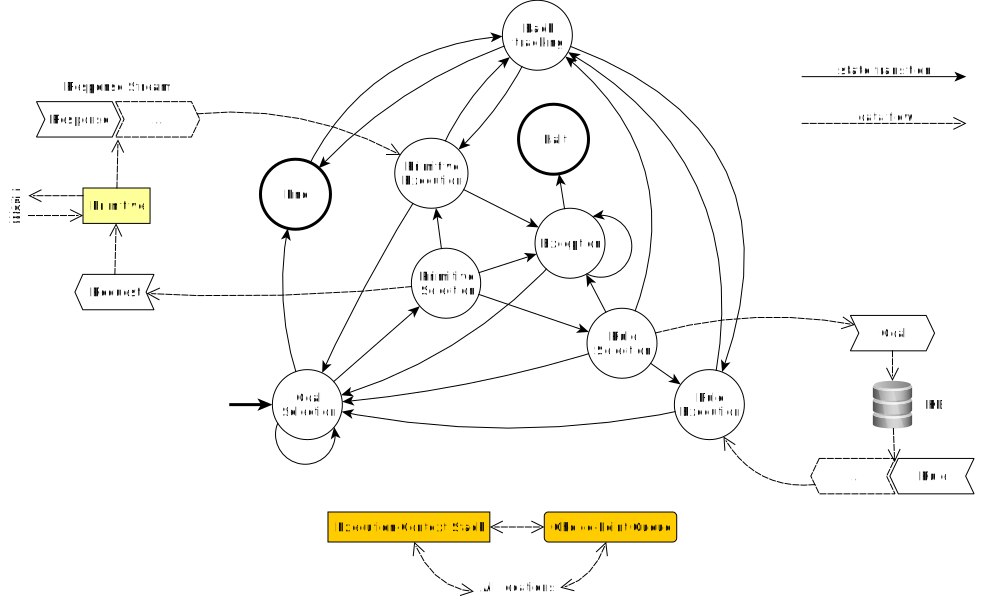
\includegraphics[width=\linewidth]{figures/2p-fsa-dataflow}
    \caption[The primitive-enabled state machine governing Prolog solvers' behaviour]{The primitive-enabled state machine governing Prolog solvers' behaviour. Location \state{Goal Selection} is the initial one, whereas \state{End} and \state{Halt} are the final ones. Location \state{Primitive} (resp. \state{Rule}) \state{Selection} is where primitives (resp. KB) are triggered (resp. queried) and their data streams are opened. Conversely, location \state{Primitive} (resp. \state{Rule}) \state{Execution} is where response (resp. clause) streams are lazily consumed}
    \label{fig:prolog-fsa}
\end{figure}

In order to design a Prolog solver supporting our notion of primitive, we enhance the Prolog state machine proposed in \cite{tuprolog-sac08} with the capability of lazily consuming streams of data coming from either a primitive or the KB (\cref{fig:prolog-fsa}).
%
In particular, we change how the state machine manages the resolution of (sub-)goals, by supporting the selection of a primitive as a means to provide one or more solutions for (sub-)goals, other than the ordinary selection of rules from the KB.

The state machine in \cref{fig:prolog-fsa} stems from the acknowledgement that a Prolog solver may solve a (sub-)goal by either selecting a primitive or a number of logic rules from the KB.
%
In both cases, a stream of data must be lazily consumed by the solver---either carrying primitive responses or clauses from the KB.

Whenever a stream of data needs to be processed, there are essentially two major phases: the \emph{opening} of the stream -- where a channel between the stream producer and its consumer is created --, and the \emph{consumption} of the stream---where items from the stream are sequentially processed.
%
To support both phases, two more locations are included -- namely \state{Primitive Selection} and \state{Primitive Execution} -- respectively aimed at triggering a primitive and consuming the response stream it provides.
%
Furthermore, to support a stream-oriented interaction among the solver and its KB, we model rule management as well through two locations, namely \state{Primitive Selection} and \state{Primitive Execution}, respectively aimed at querying the KB, and consuming the rule stream it provides.

All the other aspects are handled in the same way as in \cite{tuprolog-sac08}.
%
Thus, state machine execution is triggered whenever a user submits a query to the solver: when this is the case, execution starts from the \state{Goal Selection} location.
%
Then, it may go through any location until it eventually reaches some \emph{final} one (\state{End} or \state{Halt}), where a new solution is yielded---which the user can eventually consume.
%
Once a solution is consumed, the user can either submit a new query or ask for the next solution.
%
In the former case, the automaton is reset to the \state{Goal Selection} location.
%
Conversely, the latter case is only possible if the last solution was provided by the \state{End} location.
%
In that case, the automaton backtracks and looks for the next solution.
%
This may involve stepping through \state{Backtracking}, then moving back into the \state{Primitive} (resp. \state{Rule}) \state{Execution}, in order to consume one more element from some previously-opened response (resp. clause) stream.

Overall, our state machine affects the operation of a Prolog solver as follows:
%
\begin{enumerate}
    \item $\left[\state{Primitive Selection}\right]$ whenever a new sub-goal is selected, the solver looks for a primitive whose signature matches the sub-goal one;

    \item $\left[\state{Primitive Execution}\right]$ if some are found, the solver considers the first response in the stream as a solution to the goal, and generates choice points for subsequent responses;

    \item $\left[\state{Rule Selection}\right]$ otherwise, if no primitive is selected for the current sub-goal, some rule is looked for instead, whose head unifies with the sub-goal;

    \item $\left[\state{Rule Execution}\right]$ if any such rule is found, resolution can proceed by addressing the rule's body as the next goal to be proved;

    \item $\left[\state{Backtracking}\right]$ otherwise, if no rule is found, the sub-goal is considered failed and resolution must backtrack.
\end{enumerate}
%
Location \state{Exception} completes the picture by intercepting exceptions -- possibly thrown by primitives as part of some response of theirs --, via the standard \prolog{catch/3} predicate.

Ordinary Prolog built-in primitives naturally fit the picture as they are re-interpreted as  primitives by solvers.
%
For instance, the \texttt{is/2} predicate can be considered a functional primitive accepting a variable and an expression and returning a single response assigning the variable to the value attained by reducing the expression -- if possible --, or an exception---in case the expression cannot be reduced.
%
Conversely, the \prolog{member/2} predicate can be considered as a relational primitive, enumerating all the possible items in a list.
%
Accordingly, the aforementioned \state{Primitive Selection} location is where built-in primitives are selected for execution in place of rules from the KB.

\subsection{Formal Description}

In the reminder of this section we formally define the behaviour of a primitive-enabled state machine for Prolog.
%
The discussion starts by introducing the basic notations, functions, and data structures aimed at formally describing the semantics of our state machine.
%
Semantics is then provided via labelled transition systems.

%-----------------------------------------------------------------------------------------------%
\subsubsection{Syntax and Notational Conventions}
%-----------------------------------------------------------------------------------------------%

Here we recap the fundamental syntactical definitions our discussion relies upon.
%
Most definitions here rely on the theoretical background provided in \cref{sec:symbolic-kr}.

%-----------------------------------------------------------------------------------------------%
\paragraph{Knowledge Bases}
%-----------------------------------------------------------------------------------------------%

Let $\notableset{A}$ be the set of all atomic logic formul\ae, and let $\notableset{H}$ be the set of all well-formed Horn clauses in the form:
%
\[ a \leftarrow a_1, \ldots, a_n \quad \text{s.t.} \ n > 0\]
%
(a.k.a. rules) where $a, a_1, \ldots, a_n \in \notableset{A}$ are logic predicates of arbitrary arity.
%
Let us enumerate rules in $\notableset{H}$ by $h$.
%
Thus, we define knowledge bases as ordered containers of rules of the form $[h_1, h_2, \ldots]$.

Let $K$ denote the knowledge base, with $K \in \notableset{H}^* $, where $\notableset{H}^*$ is the set of all possible KB.

Finally, let $ \f{get} : \notableset{H}^* \times \notableset{H} \rightarrow \notableset{H}^* $ be a function defined as follows:
%
\[ \fx{get}{K, h} = \begin{cases}
    [h' \mid \fx{get}{K'}] & \text{if}\ K \equiv [h' \mid K'] \wedge \fx{mgu}{h, h'} \neq \bot \\
    [\fx{get}{K'}] & \text{if}\ K \equiv [h' \mid K'] \wedge \fx{mgu}{h, h'} = \bot \\
    [] & \text{if}\ K \equiv []
\end{cases} \]
%
aimed to select all rules in $K$ unifying with the clause $h$.

%-----------------------------------------------------------------------------------------------%
\paragraph{Primitives}
%-----------------------------------------------------------------------------------------------%

Let $\notableset{F}$ be the set of all predicate symbols, enumerated by $f$, and let $\mathbb{N}$ be the set of natural numbers.
%
Thus,
\begin{itemize}
    \item let $\notableset{F} \times \mathbb{N}$ denote the set of all possible signatures and
    \item let $(f,n) \in \notableset{F} \times \mathbb{N}$ denote the generic signature of a $n$-ary predicate whose functor is $f$.
\end{itemize}
%
Let us define the function $ \f{signature} : \notableset{A} \rightarrow \notableset{F} \times \mathbb{N} $ as:
%
\[ \fx{signature}{f(t_1, \ldots, t_n)} = (f,n) \]
%
that computes the signature of any possible atomic predicate.


Let $\Theta$ be the set of all possible substitutions -- including the failed substitution $\bot$, the empty unifier $\varnothing$, and any unifier in the form $\{V_1 \mapsto t_1, V_2 \mapsto t_2, \ldots\}$ where $V_i$ are logic variables and $t_i$ are logic terms -- and let us enumerate elements in $\Theta$ by $\theta$.

Let then $\notableset{X}$ be the set of all possible \emph{exceptions} -- i.e., arbitrary terms describing error situations --, enumerated by $x$.

Accordingly, $\notableset{R} = \notableset{X} \cup \Theta$ represents the set of all possible primitive \emph{responses}, enumerated by $r$.

Then, let $\notableset{P}$ be the set of all possible primitives with the form:
%
\[ p : \notableset{H}^* \times \notableset{A} \rightarrow \notableset{R}^* \]
%
In other words, we call ``primitive'' any function $p \in \notableset{P}$ accepting a knowledge base $K \in \notableset{H}^*$ and a goal $a \in \notableset{A}$ as input and producing a stream of responses $p(K, a) = \stream{r} \in \notableset{R}^*$ as output---where each response $r \in \stream{r}$ may either be a substitution or an exception.

Finally, we define a primitive store $I$ as a relation of the form:
%
\[ I \subseteq \notableset{F} \times \mathbb{N} \times \notableset{P} \]
%
that is, any possible indexing of primitives by signatures.
%
Given a particular primitive store $I$, we enumerate its elements by $(f, n, p)$.

%-----------------------------------------------------------------------------------------------%
\paragraph{Solver Automaton}
%-----------------------------------------------------------------------------------------------%

We define an \emph{execution context} $E$ as a tuple of the form $\left( \theta, \stream{a}, \stream{h}, \stream{p} \right)$ where:
%
\begin{itemize}
    \item $\theta \in \Theta$ is a substitution;
    \item $\stream{a} \in \notableset{A}^*$ is a stream of \emph{goals};
    \item $\stream{h} \in \notableset{H}^*$ is a stream of \emph{rules};
    \item $\stream{r} \in \notableset{R}^*$ is a stream of primitive \emph{responses}.
\end{itemize}
%
Accordingly, letting $\notableset{E}$ denote set of all possible execution contexts, we define an execution-context \emph{stack} $\vect{E}$ as a list of the form $[E_0, E_1, \ldots] \in \notableset{E}^*$, where $E_0$ can either be called the ``\emph{current} execution context'' or the ``\emph{top} of the execution-context stack''.

Conversely, we define a \emph{choice point} $C$ as any item in $\notableset{E}^*$---i.e., a snapshot of a \emph{whole} execution-context stack.
%
We then define a choice-point \emph{queue} $\vect{C}$ as a list of the form $[C_0, C_1, \ldots]$, and we denote by $\notableset{C}^*$ the set of all possible choice-point queues.
%
There, $C_0$ can either be called the ``\emph{next} choice point'' or the ``\emph{head} of the choice-point queue''.
%
Let $ \f{append} : \notableset{C}^* \times \notableset{E}^* \rightarrow \notableset{C}^* $ be a function defined as:
%
\[
\fx{append}{\vect{C}, C} = \begin{cases}
    [C] & \ \text{if}\ \vect{C} \equiv [] \\
    [C_1, \ldots, C_n, C] & \ \text{if}\ \vect{C} \equiv [C_1, \ldots, C_n] \\
\end{cases}
\]
%
serving the purpose of appending a new choice point at the end of a choice-point queue.

Finally, let $\notableset{L}$ denote the set containing all the locations depicted in \cref{fig:prolog-fsa}:
%
\begin{multline*}
    \notableset{L} = \{ \state{Goal Selection}, \state{Primitive Selection}, \state{Primitive Execution}, \state{Rule Selection},
    \\
    \state{Rule Execution}, \state{Backtracking}, \state{Exception}, \state{End}, \state{Halt} \}
\end{multline*}
%
We enumerate items in $\notableset{L}$ by $L$.

%-----------------------------------------------------------------------------------------------%
\subsubsection{Semantics}
%-----------------------------------------------------------------------------------------------%

The semantics of our Prolog state machine can be described in terms of \emph{states} and \emph{transitions} between them.
%
In this regard, a \emph{state} is a tuple of the form $\langle L, \vect{E}, \vect{C} \rangle$ where
%
\begin{itemize}
    \item $L \in \notableset{L}$ is a location,
    \item $\vect{E} \in \notableset{E}^*$ is an execution-context stack,
    \item $\vect{C} \in \notableset{C}^*$ is a choice-point queue.
\end{itemize}

Accordingly, the state machine semantics is defined as a \emph{labelled transition system} $\langle \notableset{S}, \Lambda, s_0, \longrightarrow \rangle$ where:
%
\begin{itemize}
    \item $\notableset{S}$ is the set of all possible states,
    \item $\Lambda = \{ \tau \} \cup \notableset{X} \cup \Theta $ is a set of labels,
    \item $s_0 \in \notableset{S}$ is the initial state,
    \item $\longrightarrow \subseteq \notableset{S} \times \Lambda \times \notableset{S}$ is a transition relation dictating how state may evolve in time.
\end{itemize}
%
There, transition labels in $\Lambda$ denote relevant observable events, while the anonymous label $\tau$ denotes internal events.
%
Observable events of interest can be, for instance, the production of either a positive or negative solution -- denoted by the corresponding substitution in $\Theta$ -- or the production of an exceptional solution---denoted by the corresponding exception in $\notableset{X}$.
%
In the following, for the sake of notation simplicity, we write $s \transition{\lambda} s'$ instead of $(s, \lambda, s')$ to refer to transitions in $\longrightarrow$.

Assuming that a KB $K$ and a primitive store $I$ are provided, and that the initial state $s_0 \in \notableset{K}$ is always a tuple of the form:
%
\[ \langle \state{Goal Selection},\   [( \varnothing, [g_0], [], [] )],\  [] \rangle \]
%
for some initial goal $g_0$ -- meaning that
%
\begin{inlinelist}
    \item the initial location is always \state{Goal Selection},
    \item the current context initally only contains the empty unifier $\varnothing$ and $g_0$, and
    \item the choice-point queue is initially empty
\end{inlinelist}
%
-- we can \emph{intensionally} define the admissible transitions in $\longrightarrow$ via the following transition rules---each one corresponding to an arrow in \cref{fig:prolog-fsa}.

\paragraph{Goal Selection}

The purpose of the \state{Goal Selection} location is to decide what to do next depending on which and how many (sub-)goals are in the current execution context.
%
There are three relevant situations handled in this location, by as many transition rules.
%
More precisely, if the current execution context does not contain any goals, this implies either that a new solution should be yielded, or the top execution context should be popped from the stack.
%
Conversely, if the current execution context does hold at least one goal, the automaton commits to that goal---meaning that it tries to prove its truth via subsequent transitions.

Accordingly, the following transition rule handles the case where there is only one last execution context on the stack with no more goals---thus, implying the automaton should move into the \state{End} location and a new solution should be yielded:
%
%More formally:
\[
\frac{
    E = (\theta, [], [], [])
}{
    \langle \state{Goal Selection}, [E], \vect{C} \rangle
    \transition{\theta}
    \langle \state{End}, [E], \vect{C} \rangle
}
\]
The positive or negative solution depends on the $\theta$ substitution of the last execution context $E$, which can be either a unifier or the failed substitution $\bot$.
In the former case, $\theta$ synthesises all the variable assignments computed so far by the automaton.

Conversely, the following transition rule handles the case where the current execution context has no more goals, but the stack contains
more execution contexts.
%
When this is the case, the automaton simply pops the current execution context from the stack and holds the \state{Goal Selection} location:
\[
\frac{
    E_0 = (\theta_0, [], [], [])
    \qquad
    E_1 = (\theta_0, \stream{g}, [], [])
    \qquad
    E'_1 = (\theta_1, \stream{g}, [], [])
}{
    \langle \state{Goal Selection}, [E_0, E_1 \mid \vect{E}], \vect{C} \rangle
    \transition{\tau}
    \langle \state{Goal Selection}, [E'_1 \mid \vect{E}], \vect{C} \rangle
}
\]
%
Before popping the current execution context $E_0$, the automaton spreads its $\theta_0$ substitution to the parent execution context $E_1$---as $\theta_0$ can contain more assignments than $\theta_1$.

Finally, the following transition rule handles the case in which the current execution context contains a non-empty stream of goals $\stream{g}$.
%
When this is the case the automaton applies the most recent substitution $\theta$ to all the goals in $\stream{g}$ before moving into \state{Primitive Selection} location and tries then to prove the truth of the first sub-goal in $\stream{g}$:
%
\[
\frac{
    E = (\theta, \stream{g}, [], [])
    \qquad
    E' = (\theta, \stream{g}', [], [])
    \qquad
    \stream{g}' = \apply{\stream{g}}{\theta}
}{
    \langle \state{Goal Selection}, [E \mid \vect{E}], \vect{C} \rangle
    \transition{\tau}
    \langle \state{Primitive Selection}, [E' \mid \vect{E}], \vect{C} \rangle
}
\]
%
where by $\apply{\stream{g}}{\theta}$ we mean the application of substitution $\theta$ to all goals in $\stream{g}$.


\paragraph{Primitive Selection}

The purpose of the \state{Primitive Selection} location is to select a primitive in the primitive store $I$ in order to prove a (sub-)goal---provided a primitive matching the goal's signature exists in $I$.
%
If this is the case, the primitive is triggered and the \emph{first} primitive response is handled.
%
Thus, there are three relevant situations handled in this location, by as many transition rules.
%
A pivotal role in discriminating among situations is played by the first goal $g$ of the current execution context.
%
If primitive $p$ is indexed in $I$ via signature of $g$, then $p$ is triggered and a response stream is generated in return.
%
Only the first item in the stream, $r$, is consumed.
%
This can be either an exception or a substitution. Each case is handled by a different transition rule.
%
Otherwise, if the signature of $g$ matches no primitive in $I$, no primitive is selected and, via subsequent transitions, a rule for the same goal is searched.

In particular, the following transition rule handles the case where a primitive $p$ is found in $I$ and the first response $r$ is a substitution.
%
When this is the case, a new execution context is pushed on the stack -- for handling the first response --, and a new choice point is appended to queue---for handling any further response.
%
After that, the automaton moves to the \state{Primitive Execution} location.
%
\[
\frac{
    \begin{array}{c}
        E_0 = (\theta, \stream{g}, [], [])
        \quad
        \stream{g} = [g \mid \stream{g}']
        \quad
        (f, n) = \fx{signature}{g}
        \quad
        (f, n, p) \in I
        \quad
        [r \mid \stream{r}] = p(K, g)
        \\
        r \in \Theta
        \quad
        E_1 = (\theta, \stream{g}, [], [r \mid \stream{r}'])
        \quad
        E_2 = (\theta, \stream{g}, [], \stream{r}')
        \quad
        \vect{C}' = \fx{append}{\vect{C}, [E_2, E_0 \mid \vect{E}]}
    \end{array}
}{
    \langle \state{Primitive Selection}, [E_0 \mid \vect{E}], \vect{C} \rangle
    \transition{\tau}
    \langle \state{Primitive Execution}, [E_1, E_0 \mid \vect{E}], \vect{C}' \rangle
}
\]
%
% This implies that there could be other responses in the response stream.
%
% For this reason, a novel choice point is appended to the choice-point queue.
%
% After that, the automaton moves to the \state{Primitive Execution} location.%

Conversely, the following transition rule handles the case in which the first primitive response $r$ is an exception.
%
This implies that there could \emph{not} be any further response in the response stream and the exception needs to be handled.
%
For this reason, the automaton moves into the \state{Exception} location leaving the choice-point queue unaffected:
%
\[
\frac{
    \begin{array}{c}
        E_0 = (\theta, [g \mid \stream{g}'], [], [])
        \quad
        (f, n) = \fx{signature}{g}
        \quad
        (f, n, p) \in I
        \\
        \left[x \mid \stream{r}\right] = p(K, g)
        \quad
        x \in \notableset{X}
        \quad
        E_1 = (\theta, [g \mid \stream{g}'], [], [x \mid \stream{r}])
    \end{array}
}{
    \langle \state{Primitive Selection}, [E_0 \mid \vect{E}], \vect{C} \rangle
    \transition{\tau}
    \langle \state{Exception}, [E_1, E_0 \mid \vect{E}], \vect{C} \rangle
}
\]
%
In this case as well a new execution context is pushed on the stack -- in order to make the exception visible in \state{Exception} --, whereas no new choice point is created.

Finally, the following transition rules handle the case in which a primitive is available in $I$ for the goal $g$.
%
When this is the case, the automaton simply moves into the \state{Exception} location:
%
\[
\frac{
    E = (\theta, [g \mid \stream{g}'], [], [])
    \qquad
    (f, n) = \fx{signature}{g}
    \qquad
    (f, n, p) \not\in I
}{
    \langle \state{Primitive Selection}, [E \mid \vect{E}], \vect{C} \rangle
    \transition{\tau}
    \langle \state{Rule Selection}, [E \mid \vect{E}], \vect{C} \rangle
}
\]

\paragraph{Primitive Execution}

The purpose of the \state{Primitive Execution} location is to \emph{lazily} handle the response streams produced by primitives.
%
To this regard, there are three relevant situations, handled by as many transition rules.
%
In fact, while consuming a stream of solution responses, the automaton may either encounter an empty stream, or a stream whose first element is either an exception, or a substitution.
%
The latter case is the most interesting one, as the substitution must be kept into account in the next computational steps.
%
Conversely, in the other cases, the response stream is interrupted, even if with different outcomes: while the lack of responses simply provokes backtracking, exceptions need to be handled accordingly.

In particular, the following transition rule handles the case where the first response in the stream is a unifier $\theta'$.
%
When this is the case, $\theta'$ is merged with the current execution context substitution $\theta$ and execution proceeds in the \state{Goal Selection} location.
%
\[
\frac{
    E = (\theta, [g \mid \stream{g}], [], [\theta', \ldots])
    \qquad
    \theta' \in \Theta - \{ \bot \}
    \qquad
    E' = (\theta \cup \theta', \stream{g}, [], [])
}{
    \langle \state{Primitive Execution}, [E \mid \vect{E}], \vect{C} \rangle
    \transition{\tau}
    \langle \state{Goal Selection}, [E' \mid \vect{E}], \vect{C} \rangle
}
\]
%
It is worth to highlight how this transition rule simply consumes a \emph{single} response in the stream.
%
Subsequent responses may be consumed after backtracking.
%
Thus, this is where the lazy semantics of primitives is realised.

Conversely, the following transition rule handles both the case where the first response in the stream is a failure (i.e. $\bot$), and the case of any empty response stream.
%
In all such cases, the automaton simply moves into the \state{Backtracking} location.
\[
\frac{
    E = (\theta, \stream{g}, [], \stream{r})
    \qquad
    \stream{r} = [\bot, \ldots] \lor \stream{r} = []
    \qquad
    E' = (\theta, \stream{g}, [], [])
}{
    \langle \state{Primitive Execution}, [E \mid \vect{E}], \vect{C} \rangle
    \transition{\tau}
    \langle \state{Backtracking}, [E' \mid \vect{E}], \vect{C} \rangle
}
\]

Finally, the following transition rule handles the case where the first response in the stream is an exception.
%
When this is the case, the automaton simply moves into the \state{Exception} location.
\[
\frac{
    E = (\theta, \stream{g}, [], [x, \ldots])
    \qquad
    x \in \notableset{X}
    \qquad
    E' = (\theta, \stream{g}, [], [x])
}{
    \langle \state{Primitive Execution}, [E \mid \vect{E}], \vect{C} \rangle
    \transition{\tau}
    \langle \state{Exception}, [E' \mid \vect{E}], \vect{C} \rangle
}
\]

\paragraph{Rule Selection}

The \state{Rule Selection} location is for clauses what the \state{Primitive Selection} location is for primitives.
%
It aims at querying the KB and selecting the rules to be executed to prove a particular (sub-)goal true, provided that no primitive has been selected to the purpose.
%
Accordingly, three transition rules are defined, each one handling a particular situation.
%
The most common situation here is that a number of rules $\stream{r}$ are selected from $K$ in order to solve some goal $g$.
%
However, there is a small set of goals for which a particular treatment is reserved.
%
These are: \texttt{!} (the ``cut''), \texttt{true}, \texttt{fail}, and \texttt{false}.
%
The first two are always considered successful, while the others are always considered failed.

More precisely, the following transition rule takes care of goals such as \texttt{!} and \texttt{true}.
%
As they must always be evaluated successfully, this transition simply makes the automaton move into the \state{Goal Selection} location, after consuming the current goal $g_0$.
%
However, in the particular case of $g_0 \equiv \mathtt{!}$, the transition rule also provokes the \emph{cut} of all choice points, up to the one relative to goal $g_1$ (included):
%
%More formally:
%
\[
\frac{
    \begin{array}{c}
        E_0 = (\theta_0, [g_0 \mid \stream{g}_0], [], [])
        \qquad
        g_0 \in \{ \mathtt{true}, \mathtt{!} \}
        \qquad
        E_1 = (\theta_1, [g_1, \ldots], \ldots)
        \\
        E'_0 = (\theta_0, \stream{g}_0, [], [])
        \qquad
        \vect{C}' = \fx{cut}{C, g_1}
    \end{array}
}{
    \langle \state{Rule Selection}, [E_0, E_1 \mid \vect{E}], \vect{C} \rangle
    \transition{\tau}
    \langle \state{Goal Selection}, [E'_0, E_1 \mid \vect{E}], \vect{C}' \rangle
}
\]
%
where $\f{cut} : \notableset{C^*} \times \notableset{A} \rightarrow \notableset{C^*}$ is the function cutting off choice points, up to a given goal.

Conversely, the following transition rule takes care of goals such as \texttt{fail} and \texttt{false}.
%
As they must always be evaluated successfully, this transition simply makes the automaton move into the \state{Backtracking} location, after consuming the current goal $g$.
%
This transition rule also handles the case where $K$ is queried for all rules whose head unifies with the current goal $g$, but no one is found.
%
\[
\frac{
    E = (\theta, [g, \ldots], [], [])
    \qquad
    g \in \{ \mathtt{false}, \mathtt{fail} \} \lor \fx{get}{K, g} = []
}{
    \langle \state{Rule Selection}, [E \mid \vect{E}], \vect{C} \rangle
    \transition{\tau}
    \langle \state{Backtracking}, [E \mid \vect{E}], \vect{C} \rangle
}
\]

Finally, the following transition rule handles the general case where $K$ is queried for all rules $\stream{h}$ whose head unifies with the current goal $g$.
%
Assuming that $\stream{h}$ contains at least one rule $h$, the automaton must then move to location \state{Rule Execution}, after pushing a new execution context on the stack -- aimed at handling $h$ --, and adding a new choice point to the queue---aimed at handling any further rule in $\stream{h}$:
%
%More formally:
%
\[
\frac{
    \begin{array}{c}
        E_0 = (\theta, \stream{g}, [], [])
        \quad
        \stream{g} = [g \mid \stream{g}']
        \quad
        g \in \notableset{A} - \{ \mathtt{true}, \mathtt{false}, \mathtt{fail}, \mathtt{!} \}
        \\
        \fx{get}{K, g} = \stream{h}
        \quad
        \fx{refresh}{\stream{h}} = [h \mid \stream{h}']
        \\
        E_1 = (\theta, \stream{g}, [h \mid \stream{h}'], [])
        \quad
        E_2 = (\theta, \stream{g}, \stream{h}', [])
        \quad
        \vect{C}' = \fx{append}{\vect{C}, [E_2, E_0 \mid \vect{E}]}
    \end{array}
}{
    \langle \state{Rule Selection}, [E_0 \mid \vect{E}], \vect{C} \rangle
    \transition{\tau}
    \langle \state{Rule Execution}, [E_1, E_0 \mid \vect{E}], \vect{C}' \rangle
}
\]
%
where $\f{refresh} : \notableset{H}^* \rightarrow \notableset{H}^*$ is a function refreshing all variables of all clauses in a clause stream/list.

\paragraph{Rule Execution}

The \state{Rule Execution} location is for clauses what the \state{Primitive Execution} location is for primitives.
%
Thus, the purpose of this location is to \emph{lazily} handle the rule streams produced by KB.
%
Accordingly, two transition rules are defined, each one handling a particular situation.
%
In both situations, the current execution context is assumed to carry a non-empty rule stream to be handled.
%
One situation concerns the case where the first rule in the stream has a head matching the current context goal.
%
In this case, the execution can go on and focus on the body of that rule.
%
The other situation concerns the opposite case, where execution must proceed with backtracking.
%
% In any case, the automaton cannot be in location \state{Rule Execution} while the rule stream of the execution context is empty.

Accordingly, the following transition rule handles the first situation.
%
The current execution context's first goal is $g$ and the first rule is $h$.
%
Provided that the head of $h$ unifies with $g$, and letting $\theta'$ be their unifier, the current execution context is updated in such a way that the new substitution is $\theta \cup \theta'$ and the new goal stream contains all the atoms from the body of $h$, subject to the substitution $\theta'$.
%
After that, the automaton moves to the \state{Goal Selection} location.
\[
\frac{
    \begin{array}{c}
        E = (\theta, [g \mid \stream{g}], [h, \ldots], [])
        \quad
        h = (a \leftarrow a_1, \ldots, a_n)
        \quad
        \theta' = \fx{mgu}{g, a} \neq \bot
        \\
        E' = (\theta \cup \theta', [\apply{g_1}{\theta'}, \ldots, \apply{g_n}{\theta'}], [], [])
    \end{array}
}{
    \langle \state{Rule Execution}, [E \mid \vect{E}], \vect{C} \rangle
    \transition{\tau}
    \langle \state{Goal Selection}, [E' \mid \vect{E}], \vect{C} \rangle
}
\]

Conversely, the following transition rule handles the case where the head of $h$ does not unify with $g$.
%
In this case, the automaton simply moves into the \state{Backtracking} location.
%
\[
\frac{
    E = (\theta, [g \mid \stream{g}], [h, \ldots], [])
    \quad
    h = (a \leftarrow \ldots)
    \quad
    \fx{mgu}{g, a} = \bot
    \quad
    E' = (\theta, [g \mid \stream{g}], [], [])
}{
    \langle \state{Rule Execution}, [E \mid \vect{E}], \vect{C} \rangle
    \transition{\tau}
    \langle \state{Backtracking}, [E' \mid \vect{E}], \vect{C} \rangle
}
\]

\paragraph{Backtracking}

The \state{Backtracking} location is the key point where the lazy consumption of rules and responses streams is performed by Prolog solvers.
%
More precisely, this is where the choice points previously accumulated by the automaton in the choice-points queue are handled.
%
Following this purpose, the \state{Backtracking} location may encounter three relevant situations, all depending on the content of the queue.
%
The first situation concerns the case of the queue is empty, meaning that a new negative solution should be produced by the solver.
%
The other situations concern the cases where the next choice point is carrying a non-empty rule or primitive response stream, respectively.
%
In these cases, the automaton should move into either the \state{Rule} or \state{Primitive Execution} locations, in order to go on with resolution and consume the next rule or response.

Accordingly, the following rule handles the case where the choice-point queue is empty and the and the automaton should just move into the \state{End} final location, yield a new negative solution $\bot$.
%
\[
\frac{
    %
}{
    \langle \state{Backtracking}, \vect{E}, [] \rangle
    \transition{\bot}
    \langle \state{End}, \vect{E}, [] \rangle
}
\]

Conversely, the following rule handles the case where the next choice point $C$ in the queue is an execution context carrying a non-empty primitive response stream $\stream{r}$.
%
When this is the case, the automaton simply adopts $C$ as the next execution context, popping it from the choice-point queue and moving into the \state{Primitive Execution} location.
%
\[
\frac{
    C = [(\theta, \stream{g}, [], \stream{r}), \ldots]
    \qquad
    \stream{r} \neq []
}{
    \langle \state{Backtracking}, \vect{E}, [C \mid \vect{C}] \rangle
    \transition{\tau}
    \langle \state{Primitve Execution}, C, \vect{C} \rangle
}
\]

Finally, the following rule handles the case where the next choice point $C$ in the queue is an execution context carrying a non-empty rule stream $\stream{h}$.
%
When this is the case, the automaton simply adopts $C$ as the next execution context, popping it from the choice-point queue and moving into the \state{Rule Execution} location.
%
\[
\frac{
    C = [(\theta, \stream{g}, \stream{h}, []), \ldots]
    \qquad
    \stream{h} \neq []
}{
    \langle \state{Backtracking}, \vect{E}, [C \mid \vect{C}] \rangle
    \transition{\tau}
    \langle \state{Rule Execution}, C, \vect{C} \rangle
}
\]

\paragraph{Exception Handling}

The \state{Exception} location has the purpose of managing exceptions possibly raised by primitive responses in the Standard Prolog way---i.e. by climbing the proof tree towards the root, looking for a \prolog{catch/3} (sub-)goal whose second argument unifies with the raised exception and setting its third argument as the next sub-goal to be proved.

Following this purpose, the \state{Exception} location may encounter two notable situations.
%
In both ones, the current execution is assumed to be carrying an exception $x \in \notableset{X}$.
%
The first situation concerns the case where the exception can be \emph{caught} since there exists on the stack an execution context of the form \prolog{catch/3} which may intercept the exception and let resolution continue.
%
The second situation concerns the opposite case where the exception \emph{cannot} be caught -- since no such an execution context is contained into the stack -- and resolution must be therefore interrupted.

In particular, the following transition rule handles the first situation where an execution context $E'$ exists on the stack whose first goal is $\mathtt{catch}(g_1, g_2, g_3)$.
%
When this is the case, we denote by $\theta'$ the MGU among $x$ and $g_2$.
%
Then, the automaton pops from the stack all execution contexts up to $E'$ (included), pushes a new execution context carrying $g_3$ as the first goal, and moves into the \state{Goal Selection} location.
%
\[
\frac{
    \begin{array}{c}
        E = (\theta, [g \mid \stream{g}], [], [x, \ldots])
        \quad
        x \in \notableset{X}
        \quad
        E' = (\vartheta, [\mathtt{catch}(g_1, g_2, g_3), \ldots], \stream{h}, \stream{r})
        \\
        \theta' = \fx{mgu}{x, g_2} \neq \bot
        \quad
        \theta'' = \vartheta \cup \theta'
        \quad
        E'' = (\theta'', [g_3 / \theta''], [], [])
    \end{array}
}{
    \langle \state{Exception}, [E, \ldots, E' \mid \vect{E}], \vect{C} \rangle
    \transition{\tau}
    \langle \state{Goal Selection}, [E'' \mid \vect{E}], \vect{C} \rangle
}
\]

Conversely, the following transitions rule handles the opposite situation where no execution context on the stack carries $\mathtt{catch}(g_1, g_2, g_3)$ as the first goal---or, if it does, $g_2$ does not unify with $x$.
%
When this is the case, the automaton simply moves into the \state{Halt} location, yielding an exceptional solution to the users.
%
\[
\frac{
    \begin{array}{c}
        E = (\theta, [g \mid \stream{g}], [], [x, \ldots])
        \qquad
        x \in \notableset{X}
        \\
        \vect{E} \neq [E, \ldots, (\vartheta, [\mathtt{catch}(g_1, g_2, g_3), \ldots], \stream{h}, \stream{r}), \ldots]
    \end{array}
}{
    \langle \state{Exception}, [E \mid \vect{E}], \vect{C} \rangle
    \transition{x}
    \langle \state{Halt}, [E \mid \vect{E}], \vect{C} \rangle
}
\]

\paragraph{Next Solutions}

Both the \state{End} and \state{Halt} locations are final, meaning that the automaton reaches them immediately after the production on a novel solution---be it positive, negative, or exceptional.
%
However, while the \state{Halt} location is a sink certainly provoking the automaton termination, the \state{End} state may allow the execution to be resumed.
%
In particular, when the automaton is in location \state{End}, the users may trigger the automaton again looking for further solutions---which \emph{may} be available if the choice-point queue is not empty.

Accordingly, the following transition rule handles the case where the automaton execution is resumed: once in location \state{End} the automaton may move back into location \state{Backtracking}, provided that the current choice-point queue $\vect{C}$ is non-empty.
%
\[
\frac{
    \vect{C} \neq []
}{
    \langle \state{End}, \vect{E}, \vect{C} \rangle
    \transition{\tau}
    \langle \state{Backtracking}, \vect{E}, \vect{C} \rangle
}
\]
%
Thus, the automaton actually terminates in location \state{End} only when the choice-point queue is empty.

%%%%%%%%%%%%%%%%%%%%%%%%%%%%
\section{Predicates as Streams in \twopkt{}}
%%%%%%%%%%%%%%%%%%%%%%%%%%%%

In order to demonstrate the feasibility of our approach, we propose a case study based on \twopkt{}.
%
\twopkt{} \cite{cco-softwarex-2021-2pkt} is a Kotlin-based ecosystem for LP, including general API for stream-oriented logic solvers of any sort.
%
Regardless of the particular logic, inference rule, or search strategy of choice, a logic solver is modelled in \twopkt{} as a prosumer of streams: it produces output streams of solutions and consumes input streams generated by primitives.
%
A Prolog solver implementation is available as well, leveraging the state-machine-based design presented in \cref{sec:state-machine}.
%
Furthermore, \twopkt{} involves an API for writing primitives in Kotlin, by blending an imperative, object-oriented, and functional programming style .

In this section, we first illustrate briefly the portion of the \twopkt{} API involving solvers and primitives, then we discuss an example primitive implementing the TSP example from \cref{ssec:tsp}.

\subsection{\twopkt{} Solvers and Primitives API}

Here we focus on the resolution-related portion of the \twopkt{} API (cf. \cref{chap:ecosystem} for further details).
%
There, logic solvers are modelled as instances of the \kotlin{Solver} type defined as shown in \cref{lst:interface-solver}:
%
\lstinputlisting[
    float,
    caption={Interface of a general purpose \kotlin{Solver} in \twopkt{}},
    label={lst:interface-solver},
    language=Kotlin
]{listings/Solver.kt}
%
Essentially, a logic solver is any entity exposing a method \kotlin{solve} which accepts a logic \kotlin{Struct}ure -- i.e., a particular case of logic \kotlin{Term} in the \twopkt{} type system -- as the input goal, and produces a \kotlin{Sequence} -- i.e., a \emph{lazy} stream in the Kotlin type system -- of logic \kotlin{Solution}s as output.
%
Furthermore, \twopkt{} requires each logic solver to be composed by at least three more entities, namely:
%
\begin{inlinelist}
    \item a \kotlin{staticKb} and
    \item a \kotlin{dynamicKb}, both of type \kotlin{Theory} -- that is, an ordered and indexed container of logic clauses, retrievable via unification --, and
    \item a \kotlin{libraries} container of type \kotlin{Libraries}---which, within the scope of this section, is essentially an implementation of the structure indexing primitives.
\end{inlinelist}

Each \kotlin{Solution} in \twopkt{} may be of any of three sorts, namely \kotlin{Yes}, \mbox{\kotlin{No},} and \kotlin{Halt}, representing the positive, negative, and exceptional case, respectively.
%
All solutions carry the original query they are answering to, other than the \kotlin{Substitution} they are answering through.
%
So for instance, objects of type \kotlin{Solution.Yes} always contain an object of type \kotlin{Substitution.Unifier}, whereas other sorts of solutions always contain an object of type \kotlin{Substitution.Fail}.
%
Similarly, objects of type \kotlin{Solution.Halt} carry the uncaught exception which interrupted the resolution process.

Primitives are modelled in \twopkt{} as functional interfaces, as shown in \cref{lst:interface-primitive},
%
\lstinputlisting[
    float,
    caption={Interface of a general-purpose \kotlin{Primitive} in \twopkt{}},
    label={lst:interface-primitive},
    language=Kotlin
]{listings/Primitive.kt}
%
i.e. as functions accepting a \kotlin{Request} as input and returning a \kotlin{Sequence} of \kotlin{Responses} as output.
%
There, \kotlin{Request} (cf. \cref{lst:api-request}) is a container of all the information needed at runtime to produce a sequence of \kotlin{Response}s.
%
%
\lstinputlisting[
    float,
    caption={API of a primitive's \kotlin{Request} in \twopkt{}},
    label={lst:api-request},
    language=Kotlin
]{listings/Request.kt}
%
These include:
%
\begin{inlinelist}
    \item a snapshot of \kotlin{ExecutionContext} at invocation time -- in turn including a snapshot of the solver's \kotlin{staticKb} and \kotlin{dynamicKb} --,
    \item the \kotlin{Signature} of the invoked primitive, and
    \item the \kotlin{List} of \kotlin{Terms} storing actual \kotlin{arguments} provided to the primitive upon invocation.
\end{inlinelist}
%
Furthermore, each instance of \kotlin{Request} exposes a bunch of methods -- namely, the many \kotlin{reply*()} ones --, aimed at generating a new \kotlin{Response} for that particular \kotlin{Request}.
%
As \kotlin{Response}s are mere containers of \kotlin{Solution}s, there are many variants of the \kotlin{reply*()} methods, each one aimed at generating a given sort of responses -- e.g. responses carrying positive/negative/exceptional solutions -- for the sub-goal that triggered the primitive.
%
Finally, each request supports the spawning of an inner resolution process via its \kotlin{solve(...)} method.
%
This method creates a novel sub-solver through which primitive implementers can resolve sub-queries as part of some primitive execution.

Thanks to this design, any Kotlin function of the form shown in \cref{lst:implementation-primitive}
%
\lstinputlisting[
    float,
    caption={General structure of a function acting as primitive in \twopkt{}},
    label={lst:implementation-primitive},
    language=Kotlin
]{listings/method.kt}
%
can be considered a primitive in the eyes of a logic solver.
%
This leverages a particular feature of Kotlin, namely the \kotlin{sequence \{ ... \}} blocks, which let developers write stream \emph{primitives} by blending the imperative and functional programming styles.
%
This is possible because of the \kotlin{yield(value)} method which users may call inside \kotlin{sequence \{ ... \}} blocks in place of \kotlin{return value} to provide values to the stream.

So, for instance, to implement the predicate \prolog{natural/1} -- which holds true for all natural numbers --, one may write the primitive from \cref{lst:natural-primitive}.
%
\lstinputlisting[
    float,
    caption={Implementation of a primitive aimed at lazily generating all natural numbers in \twopkt{}},
    label={lst:natural-primitive},
    language=Kotlin
]{listings/natural.kt}
%
A Prolog solver would then treat such a primitive as a backtrackable predicate.
%
Thus, in Prolog, one may use the goal \prolog{natural(X)} to enumerate all the natural numbers.
%
Similarly, to implement the predicate \prolog{even/1} -- which holds true for all \emph{even} natural numbers --, one may simply rewrite method \kotlin{natural} as follows:
%
\lstinputlisting[
    float,
    caption={Implementation of a primitive aimed at lazily generating all \emph{even} natural numbers in \twopkt{}},
    label={lst:even-primitive},
    language=Kotlin
]{listings/even.kt}

Summarising, \twopkt{} primitives API supports the creation of backtrackable Prolog predicates out of lazy data streams.

\subsection{Travelling Salesman Problem in \twopkt{}}

The real potential of primitives is revealed when they are exploited by solvers to manage input data streams from the external world.
%
There, the external world may be any source of data, there including other solvers, possibly of different nature.
%
For example, primitives may be exploited to let a Prolog solver call a TSP solver to efficiently compute solutions for TSP instances, as discussed in \cref{ssec:tsp}.
%
Accordingly, here we demonstrate how a primitive of such a sort may be realised through \twopkt{}.

In \cite{2P-Kt-TSP-Example} we provide a GitHub repository hosting the source code of a \twopkt{} primitive leveraging Google OR-Tools \cite{ortools} to efficiently solve TSP instances.
%
Google OR-Tools is a C++ library proving many constraint programming and operative research tools -- there including routing-related facilities --, and some JVM bindings which let us exploit such tools in Kotlin.

Accordingly, our repository includes some scripts aimed at automating the compilation and execution of a simple demo involving a command-line TSP-enabled Prolog interpreter.
%
Following the discussion from \cref{ssec:tsp}, such a Prolog interpreter exposes a \prolog{tsp/3} predicate aimed at enumerating the minimally-costly circuits for any given set of cities, provided that the interpreter's KB contains several \prolog{path/3} facts describing the connections among those cities.
%
As an ordinary Prolog interpreter, such facts may be either consulted from a \texttt{.pl} file or dynamically asserted via \prolog{assert/1}.

\lstinputlisting[
    float,
    basicstyle=\ttfamily\tiny,
    caption={\twopkt{} primitive implementing the \prolog{tsp/3} predicate},
    label={lst:2pkt:tsp},
    language=Kotlin
]{listings/Tsp.kt}

The actual operational behaviour of predicate \prolog{tsp/3} is governed by the \texttt{Tsp} primitive whose source code (stub) is shown in \cref{lst:2pkt:tsp} (cf. \cite{2P-Kt-TSP-Example} for full source code).
%
The \kotlin{Tsp} primitive is a singleton object of type \kotlin{TernaryRelation} -- i.e., a particular sort of \kotlin{Primitive}, tailored on ternary predicates --, whose main behaviour is encapsulated within the \kotlin{computeAll} method.

The \kotlin{Tsp} object is also endowed with a method -- namely, \kotlin{tsp} -- which returns a sequence of circuits and costs for any given list of cities provided as input.
%
Such method assumes each input city to be represented by a logic term -- in particular, a constant --, and outputs circuits represented as logic lists of cities represented in the same way.
%
Behind the scenes, the \kotlin{tsp} interacts both the Prolog interpreter's KB to read distances among cities, and a Google OR-Tool solver for computing all possible solution to a particular TSP instance.

The \kotlin{computeAll} handles the situation where the Prolog interpreter meets a (sub-)goal of the form \prolog{tsp(Cities, Circuit, Cost)}---where all variables may be partially or totally uninstantiated.
%
The method operation can then be described as a pipeline of \emph{lazy} operations applied to the actual arguments of \prolog{tsp/3}, which we refer as \kotlin{fst}, \kotlin{snd}, and \kotlin{trd} within the method.
%
Accordingly, the method firstly performs a sub-query aimed at computing the set of all cities currently contained into the KB (cf. variable \kotlin{allCities} in \cref{lst:2pkt:tsp}).
%
The sub-query is a Prolog goal of the form \prolog{path(_, _, _)}, whose solutions are all eagerly consumed and their first and second arguments -- which are assumed to be city names -- are merged into a set, to remove duplicates.
%
Then, all possible permutations of all possible subsets of \kotlin{allCities} are lazily generated.
%
However, only the subsets of cities that unify with \kotlin{fst} are actually selected (this may be just one set of cities if \kotlin{fst} refers to a fully instantiated set of cities) for the next steps of the computation.
%
Then, for all selected sets of cities, all possible solutions to the corresponding TSP instance are computed.
%
Finally, each possible circuit (resp.\ cost) computed for each TSP instance is unified with \kotlin{snd} (resp. \kotlin{trd}).
%
Failed unifications are of course dropped, while the successful ones are converted into responses of the \prolog{tsp/3} primitive.

It is worth to highlight that the whole pipeline is \emph{lazy}.
%
This implies that even once the first TSP solution has been presented to the user, the other ones are still to be computed.

%%%%%%%%%%%%%%%%%%%%%%%%%%%%
\section{Recap and Research Perspectives}
%%%%%%%%%%%%%%%%%%%%%%%%%%%%

%\note{remove recap, expand future works. mention concurrency in future works}

In this chapter we address the issue of stream processing in logic programming.

In particular, we discuss how logic solvers can be naturally conceived as lazy prosumers of data streams as they
%
\begin{inlinelist}
    \item lazily \emph{produce} data streams thanks to their interactive nature,
    \item lazily \emph{consume} data streams as part of their resolution process---e.g. when they access knowledge bases.
\end{inlinelist}
%
Furthermore, we show how logic solvers can support the processing of input data stream via the notion of predicates as \emph{primitives}, which we introduce in this chapter.
%
Summarising, primitives are reactive computational units which logic solvers may trigger so as to receive data streams from the external world.
%
This may be useful, for instance, to let a solver delegate some part of its resolution process to some external entity---assuming that it is optimised to the purpose.

To demonstrate the feasibility of our approach in the specific (and technically most relevant) case of Prolog, we propose a primitive-enabled modelling of Prolog solvers as state machines, formalising the lazy consumption of streams via backtracking.
%
The proposed formalisation preserves the standard operation of Prolog and requires no modification to the language, while enabling Prolog solvers to process data streams.

Finally, we discuss the use case of \twopkt{} \cite{cco-softwarex-2021-2pkt}, a Kotlin-based technology for LP including an implementation of Prolog solvers relying on our state-machine-based formalisation.
%
We then exploit \twopkt{} to show how primitives can be used to bridge different sorts of solvers together via a few lines of Kotlin code.

In our perspective, this work represents one further step towards the \emph{practical} exploitation of LP -- and, in particular, Prolog -- as a general means for stream processing.
%
Notably, our contribution presents some similarities with other works~\cite{Tarau2019,Redl16}.
%
In particular, similarly to~\cite{Tarau2019}, we focus on letting Prolog manipulate streams of data; while, similarly to~\cite{Redl16}, we provide a mechanism to let logic solvers delegate computations to external entities.
%
However, differently from~\cite{Tarau2019}, we require no variation to the syntax, functioning, or libraries of Prolog; while, unlike~\cite{Redl16}, we focus on Prolog rather than ASP.

A number of issues remain uncovered in this work, and will be the subject of our future research.
%
Among the many, the most relevant issues concern \emph{time}, \emph{side effects}, and \emph{concurrency}.
%
In particular we plan to explore the temporal dimension in LP-based stream processing, by providing for instance some means to support time-dependent or time-limited data streams.
%
Similarly, we would like to explore the intricacies related to the processing of data streams which may affect the internal state of a logic solver -- e.g. by affecting the KB -- in a predictable way.
%
Finally, as further discussed in \cref{sec:concurrent-lp}, we are interested developing a framework for \emph{concurrent} resolution, following the same state-machine-based approach we exploit in this chapter.

\chapter{Bridging LP and Mainstream Programming Paradigms}
\label{chap:kt-dsl}

\mypapers{kotlindsi4prolog-woa2020}

Logic Programming (LP) \cite{Apt2001,Kowalski1974} is a programming pa\-ra\-di\-gm based on formal logic, inspired to the idea of declaratively specifying a program semantics via logic formul\ae{}, so that automatic reasoners can then prove such formul\ae{} by leveraging on different \emph{control} strategies.
%
In the years, LP has contributed to the development of a number of diverse research fields laying under the umbrella of symbolic AI---such as automatic theorem proving, multi-agent systems, model checking, research optimisation, natural language processing, etc.

Nowadays, LP is one of the major programming pa\-ra\-di\-gms available for software development, along with the imperative, functional, and object-oriented ones.
%
In particular, LP is today one of the best-suited choices for tackling problems involving knowledge representation, logic inference, automated reasoning, search in a discrete space, or meta-programming \cite{logictech-information11}.
%
Moreover, today LP supports the core of AI components in pervasive and distributed systems, providing intelligence where and when it is needed \cite{microintelligencelp-mmasII}.

This is why the \emph{integration} of LP within the main programming languages is  nowadays more interesting than ever.
%
However, to make it actually work, integration should be designed -- from a linguistic standpoint -- so as to reduce both the development time and the learning curve of developers, as well as the psychological and cultural resistances against the adoption of new paradigms---thus, basically, moving LP up to a manageable level by the OOP developer.

Most mainstream programming languages -- such as Java, Kotlin, Scala, Python, JavaScript, C\# -- have recognised the added value of the integration of diverse programming paradigms under a unique syntax, a coherent API, and a rich standard library.
%
In fact, they all already support both the object-oriented (OOP) and functional (FP) programming paradigms.
%
We believe that the same languages would largely benefit from extending their support to LP languages as well, making them usable in the OOP context in the same way as FP features already are.

Interoperability among Prolog \cite{ColmerauerR93} (as the first and most prominent LP language) with other languages from different paradigms is not new: the Prolog community has actually been studying this theme for years \cite{Bagnara2002}, as shown by the many forms of integration historically present in most Prolog systems, providing either
%
\begin{inlinelist}
    \item\label{item:logic2oop} logic-to-OOP interoperability, making object orientation available within Prolog scripts, or
    \item\label{item:oop2logic} OOP-to-logic interoperability, making logic programming exploitable within object-oriented code
\end{inlinelist}%
%
---or both, as in the case of \tuprolog{} Java Library \cite{tuprolog-scp57}.
%
It is worth noting here that existing integrations make quite strong assumptions.
%
For instance, \cref{item:logic2oop} assumes the main application is written in Prolog and the interoperation is given via a suitable interface allowing the injection of (small) parts written in other languages, while \cref{item:oop2logic} implicitly assumes LP and Prolog to be somehow \emph{harmonised} with the language(s) hosting them, at the paradigm, syntactical, and technological levels.
%
Both these assumptions can actually create a barrier against an effective adoption of LP in today applications despite its huge potential.

Therefore, the approach adopted in this work is to devise instead a form of LP-FP-OOP \emph{blended integration}, such that the key features of LP paradigm can be exposed and made available to mainstream language developers in a way that is the most natural in that context.
%
The key requirement, therefore, is the ``making LP easy to adopt for OOP programmers'', in order to break down the learning curve for non-experts, and pursuit the typical developers' mindset.
%
Going beyond the mere interoperability intended as simple technical habilitation, our approach is meant to embrace the perspective of the OOP developer aiming at exploiting the potential of LP.

To this end, we show how designing Prolog as a \emph{domain-specific language} (DSL) for an OOP language such as Kotlin can make LP close enough to the OOP developers' mindset to overcome most cultural barriers, while at the same mimicking the Prolog syntax and semantics close enough to make its use straightforward for LP developers.

Generally speaking, the integration of Prolog with other paradigms aims at bringing the effectiveness and declarativeness of LP into general-purpose OOP framework.
%
In particular, OOP designers and programmers can be expected to benefit from LP features for
%
\begin{inlinelist}
    \item data-driven or data-intensive computations, such as in the case of complex-event-processing frameworks;
    \item operation research or symbolic AI algorithms, or more generally other algorithms involving a search space to be explored;
    \item multi-agent systems, and the many areas in that field leveraging on LP, such as knowledge representation, argumentation, normative systems, etc.
\end{inlinelist}

The proposed solution is based on the \twopkt{} technology \cite{homepage2PKt,cco-softwarex-2021-2pkt}, a re-engineering of the \tuprolog{} project \cite{homepageTuprolog,tuprolog-padl01} as a Kotlin multi-platform library supporting the JVM, JS, Android, and Native platforms.
%
The case of a Kotlin-based Prolog DSL is presented and discussed.

Accordingly, the chapter is organised as follows.
%
\Cref{sec:sota} briefly introduces LP, providing details about \tuprolog{}, \twopkt{}, and Kotlin as well.
%
It also summarises the current state of the integration between LP and mainstream programming languages.
%
\Cref{sec:contribution} discusses the rationale, design, and architecture of our Prolog-Kotlin DSL along with some examples.
%
\Cref{sec:case-study}, briefly illustrates a case study where our DSL is used in combination with functional programming to solve a simple AI task in an elegant way.
%
Finally, in \cref{sec:conclusions}, concludes the chapter by providing some insights about the possible future research directions stemming from our work.

\section{Background}\label{sec:sota}

\subsection{LP integration with other languages}

%The idea of integrating Prolog with high-level languages is not new.
%
%Indeed, as shown in \cref{tab:fli}, many Prolog implementations expose a \emph{foreign language interface} (FLI) towards some high-level target language.
In order to integrate LP with high-level languages, many Prolog implementations expose a foreign language interface (FLI, \cref{tab:fli}) towards some high-level \emph{target} language.
%
In most cases, the target language is Java, and the FLI is bi-directional---meaning that it supports both ``calling Prolog from the target language'' and vice versa.
%
In a few particular cases, however, the JavaScript and C\# languages are also supported.
%
As we are mostly interested in discussing how and to what extent Prolog exploitation is  possible within the target languages, in the reminder of this section we only focus on those FLI allowing to ``call Prolog from the target language''.

Each FLI mentioned in \cref{tab:fli} is characterised by a number of features that heavily impact the way the users of the target languages may actually exploit Prolog.
%
These are, for instance, the nature of the FLI -- which is tightly related to the target platform of the underlying Prolog implementation -- and its reference programming paradigm.

By ``nature'' of the FLI, we mean the technological mechanism exploited by a particular Prolog implementation to interact with the target language.
%
There are some cases -- like \tuprolog{} and $\tau$Prolog -- where this aspect is trivial, because the target language is also the implementation language---so Prolog is considered there as just another library for the target language.
%
More commonly, however, Prolog is implemented in C, and the Java Native Interface (JNI) is exploited to make it callable from Java.
%
This is for instance the case of SWI- and ECLiPSe-Prolog.
%
While this solution is very efficient, it hinders the portability of Prolog into particular contexts such as Android, and its exploitation within mobile applications.

% !TeX root = phd-thesis.tex

%\usepackage{graphicx}

\begin{table}
\caption{Prolog implementations and their foreign language interfaces (FLI)}
\label{tab:fli}
\begin{adjustbox}{width=\textwidth,center}
\begin{tabular}{c|ccccc}
\textbf{\makecell{Prolog\\Implementation}} & \textbf{Platform} & \textbf{\makecell{FLI\\towards}} & \textbf{\makecell{Nature\\of FLI}} & \textbf{\makecell{Paradigm\\of FLI}} & \textbf{Source}
%& \textbf{Homepage}
\\
\hline\hline
BProlog \cite{homepageBprolog}     & C  & Java       & JNI    & imperative & \href{http://www.picat-lang.org/bprolog/download/manual.pdf#chapter.18}{Official BProlog doc.}
%& \url{http://www.picat-lang.org/bprolog}
\\
\hline
Ciao! \cite{homepageCiao}        & C  & Java       & TCP/IP & imperative & \href{http://cliplab.org/~clip/Software/Ciao/ciao-1.15.0.html/javall_doc.html}{Official Ciao Prolog doc.}
%& \url{https://ciao-lang.org}
\\
\hline
ECLiPSe \cite{homepageEclipse}     & C  & Java       & JNI    & imperative & \href{https://eclipseclp.org/doc/javadoc/JavaEclipseInterface/index.html}{Official ECLiPSe doc.}
%& \url{https://eclipseclp.org}
\\
\hline
SICStus \cite{homepageSicstus}      & C  & Java, C\#       & TCP/IP & object-oriented & \href{https://sicstus.sics.se/sicstus/docs/latest4/html/sicstus.html/Interfacing-_002eNET-and-Java.html}{Jasper Library}
%& \url{https://sicstus.sics.se}
\\
\hline
SWI \cite{homepageSwi}         & C  & Java       & JNI    & object-oriented & \href{https://jpl7.org}{JPL API}
%& \url{https://www.swi-prolog.org}
\\
\hline
$\tau$Prolog \cite{homepageTau} & JS & JavaScript & Native & object-oriented & \href{http://tau-prolog.org}{Project homepage}
%& \url{http://tau-prolog.org}
\\
\hline
\tuprolog{} \cite{homepageTuprolog} & \makecell{JS, JVM\\ Android} & \makecell{Kotlin, Java,\\ JavaScript} & Native & \makecell{object-oriented,\\ functional} & \href{http://tuprolog.unibo.it}{Project homepage}
%& \url{http://tuprolog.unibo.it}
\\
\hline
XSB  \cite{homepageXsb}       & C  & Java       & TCP/IP & imperative & \href{http://interprolog.com/java-bridge}{Interprolog Java Bridge}
%& \url{http://xsb.sourceforge.net}
\end{tabular}%
\end{adjustbox}
\end{table}


Another viable solution is to leverage on the TCP/IP protocol stack.
%
This is for instance the case of SICStus- and Ciao-Prolog.
%
The general idea behind this approach is that the Prolog implementation acts as a remote server offering logic-programming services to the target language via TCP/IP, provided that a client library exists on the Java side making the exploitation of TCP/IP transparent to the users.
%
While this solution is more portable -- as virtually any sort of device supports TCP/IP --, it raises efficiency issues because of the overhead due to network/inter-process communications.
%
A more general solution of that sort is instead offered by the LPaaS architecture \cite{lpaas-tplp18}, where the fundamental idea is to have many Prolog engines distributed over the network, accessed as logic-based web services.
%
By the way, the implementation of LPaaS\footnote{\url{http://lpaas.apice.unibo.it}} is based on \tuprolog{}.

By ``reference programming paradigm'' of the FLI we mean the specific programming style proposed by a Prolog implementation to the target language users through its API.
%
Some FLI are conceived to be used in a strictly imperative way: this is e.g.\ the case of BProlog or Ciao! Prolog, where a Java API is available for writing Prolog queries and issue them towards the underlying Prolog system in an imperative way.
%
Other Prolog implementations, such as SICStus- and SWI-Prolog, offer a more object-oriented API which let developer not only represent queries but also terms, and solutions (there including variable bindings) which can be consumed through ordinary OOP mechanisms such as iterators.

In most cases, however, the code to be produced in the target language is far less concise and compact than pure Prolog -- unless strings and parsing are extensively adopted  --, especially when the size of the Prolog code to be represented grows.
%
So, for instance, the simple Prolog query \mbox{\texttt{?- parent(adam, X)}} (aimed at computing who Adam's son is) in Java through SWI-Prolog's JPL interface would be written as in \cref{lst:swi-fli}.
%
\lstinputlisting[
    float,
    language=Java,
    label={lst:swi-fli},
    caption={SWI-Prolog JPL interface example}
]{listings/SwiFliExample.java}
%
While this a totally effective solution on the technical level, we argue that a more convenient integration among LP and the other paradigms is possible.
%
In particular, in this chapter we show how \twopkt{} allows for a finer integration at the paradigm level through \emph{domain-specific languages}.

\subsection{Kotlin Domain-Specific Languages (DSL)}

Domain-specific languages (DSL) are a common way to tackle recurrent problems in a general way via software engineering.
%
When a software artefact (e.g. library, architecture, system) is available to tackle with  some sort of problems, designers may provide a DSL for that artefact to ease its usage for practitioners.
%
There, the exploitation of a DSL hides the complexity of the library behind the scenes, while supporting the usage of the artefact for non-expert users too.
%
This is, for instance, the approach of the Gradle build system\footnotemark---which is nowadays one of the most successful build automation systems for the JVM, Android, and C/C++ platforms.
%
\footnotetext{\url{https://gradle.org}}
%
It is also the approach followed by the JADE agent programming framework, which is nowadays usable through the Jadescript DSL \cite{BergentiCMP20}.

Building a DSL usually requires the definition of a concrete syntax, the design and implementation of a compiler or code generator, and the creation of an eco\-system of tools---e.g., syntax highlighters, syntax checkers, debuggers.
%
In particular, compilation or code generation are fundamental as they are what makes a DSL machine-interpretable and -executable.

Some high-level languages, however, such as Kotlin, Groovy, or Scala, enable a different approach.
%
They come with a flexible syntax which \emph{natively} supports the definition of new DSL with no addition to the hosting language required.
%
For instance, Gradle consists of a JVM library of methods for building, testing, and deploying sources codes, plus a Kotlin- or Groovy-based DSL allowing developers to customise their particular workflows.

The advantages of this approach are manifold.
%
First, no compiler or code generator has to be built, as the DSL is already part of the hosting language and it is therefore machine-interpretable and -executable by construction.
%
Second, the DSL automatically inherits all the constructs, API, and libraries of the hosting lan\-gua\-ge---there including conditional or iterative con\-stru\-cts, string manipulation API, etc., which are common and useful for many DSL, regardless of their particular domain.
%
Third, the ecosystem of tools supporting the hosting language -- e.g. compilers, debuggers, formatters, code analysers, IDE, etc. -- can be reused for the DSL as well, easing its adoption and making it more valuable.

When Kotlin is the hosting language of choice, DSL leverage on a small set of features making the Kotlin syntax very flexible, described below:
%
\begin{description}
    \item[operator overloading\footnotemark] --- allowing ordinary arithmetic, comparison, access, and function invocation operators to change their ordinary meaning on a per-type basis;

    \footnotetext{\url{https://kotlinlang.org/docs/reference/operator-overloading.html}}

    \item[block-like lambda expressions\footnotemark] --- including a number of syntactic sugar options such as
    %
    \begin{inlinelist}
        \item the possibility to omit formal parameters in case of a single-argument lambda expression, and
        \item the possibility to omit the round parentheses in case of a function invocation having a lambda expression as a last argument;
    \end{inlinelist}

    \footnotetext{\label{foot:lamdbda}\url{https://kotlinlang.org/docs/reference/lambdas.html}}

    \item[function types/literals with receiver\footnoteref{foot:lamdbda}] --- allowing functions and methods to accept lambda expressions within which the \texttt{this} variable references a different object than the outer scope;

    \item[extension methods\footnotemark] --- allowing pre-existing types to be extended with new instance methods whose visibility is scope-sensible.

    \footnotetext{\url{https://kotlinlang.org/docs/reference/extensions.html}}
\end{description}
%
Of course, Kotlin-based DSL automatically inherit the full gamma of facilities exposed by the Kotlin language and standard library---there including support for imperative, and object-oriented programming, as well as a rich API supporting functional programming through most common high-order operations.
%
Furthermore, if properly engineered, these DSL may be executed on all the platforms supported by Kotlin---which commonly include, at least, the JVM, JavaScript, and Android.
%
This is for instance the case of our DSL proposed in \cref{sec:contribution}.

While this chapter focuses on Kotlin-based DSL, similar results could be achieved in other languages by means of equivalent mechanisms.
%
For instance, in Scala, extension methods have to be emulated via implicit classes, and DSL, in particular, can be built via the ``Pimp My Library'' pattern \cite{Oliveira2010}.

\section{A domain-specific language for LP}\label{sec:contribution}

\subsection{Design Rationale}

Regardless of the technological choices, the design of our DSL leverages on a small set of principles ($\mathbf{P_i}$) briefly discussed below.
%
In fact, our aim is to ($\mathbf{P_1}$) provide a DSL that is a \emph{strict} extension of its hosting language, meaning that no feature of the latter language is prevented by the usage of our DSL.
%
Dually, we require ($\mathbf{P_2}$) our DSL to be fully interoperable and finely integrated with the hosting language, meaning that all the features of the latter language can be exploited from within our DSL.
%
However, we also require ($\mathbf{P_3}$) the DSL to be well encapsulated and clearly identifiable within the hosting language, in order to prevent unintended usage of the DSL itself.
%
Finally, we require ($\mathbf{P_4}$) our DSL to be as close as possible to Prolog, both at the syntactic and semantic level, to ease its exploitation for logic programmers.

In order to accomplish to the aforementioned principles, we choose the Kotlin language as the technological reference for prototyping our proposal.
%
This is because it
%
\begin{inlinelist}
    \item comes with a flexible syntax supporting the definition of DSL,
    \item supports a considerable number of platforms (JVM, JavaScript, Android, Native) and therefore enables a wide exploitation of LP -- for instance, on smart devices --,
    \item includes a number of libraries supporting LP-based applications, such as \twopkt{}.
\end{inlinelist}

\subsection{The Kotlin DSL for Prolog}\label{ssec:dsl-overview}

Before dwelling into the details of our proposal, we provide an overview of what a Kotlin DSL for Prolog has to offer.

Let us consider the Prolog theory shown in \cref{fig:relatives-prolog} describing a portion of Abraham's family tree.
%
\lstinputlisting[
    float,
    language=Prolog,
    caption={Prolog theory describing Abraham's family tree},
    label={fig:relatives-prolog}
]{listings/relatives.pl}
%
It enables a number of queries, e.g. \texttt{ancestor(a\-bra\-ham, X)}, which can be read as ``Does there exist some \texttt{X} which is a descendant of Abraham?''.
%
According to the Prolog semantics, this query may have a number of solutions, enumerating all the possible descendants of Abraham that can be deduced from the above theory---i.e., Isaac, Jacob, and Joseph.

The same result may be attained through the Kotlin program depicted in \cref{fig:relatives-kotlin}, which leverages on our DSL for Prolog:
%
%\begin{listing}[H]
\lstinputlisting[
    float,
    language=Kotlin,
    caption={Kotlin code generating the logic theory from \cref{fig:relatives-prolog}},
    label={fig:relatives-kotlin}
]{listings/Relatives.kt}
%\end{listing}
%
The program creates a Prolog solver and initialises it with standard built-in predicates.
%
Then it loads a number of facts and rules representing the aforementioned Prolog theory about Abraham's family tree.
%
Finally, it exploits the solver to find all the descendants of Abraham, by issuing the query \texttt{ancestor(abraham, X)}.

It is worth noting how the simple code snippet exemplified above is adherent w.r.t. our principles.
%
In fact, the whole DSL is \emph{encapsulated} ($\mathbf{P_3}$) within the
%
\begin{center}\ttfamily
    prolog \{ $\langle DSL\ block \rangle$ \}
\end{center}
%
In there, LP facilities can be exploited in combination with the imperative and functional constructs offered by the Kotlin language and its standard-library ($\mathbf{P_1}$ and $\mathbf{P_2}$)---such as the \texttt{for-each}-loop used to print solutions in the snippet above.
%
Furthermore, within \texttt{prolog} blocks, both theories and queries are expressed via a Kotlin-compliant syntax mimicking Prolog ($\mathbf{P_4}$).
%
The main idea behind such syntax is that each expression in the form
%
\begin{center}\ttfamily
    \kotlin{"functor"}($\langle e_1 \rangle$, $\langle e_2 \rangle$, $\ldots$)
\end{center}
%
is interpreted as a compound term (a.k.a.\ structure) in the form
$\texttt{functor}(t_1,\ t_2,\ \ldots)$,
provided that each Kotlin expression $e_i$ can be recursively evaluated as the term $t_i$---e.g. capital strings such as \kotlin{"X"} are interpreted as variables, whereas non-capital strings such as \kotlin{"atom"} (as well as Kotlin numbers) are interpreted as Prolog constants.
%
In a similar way, expressions of the form\footnote{backticks make Kotlin parse words as identifiers instead of keywords}
%
%\begin{minted}[frame=none,framesep=0mm]{kotlin}
%rule {
%  "head"(|$\langle e_1 \rangle$|, |$\ldots$|,  |$\langle e_N \rangle$|) `if` (
%    |$\langle e_{N+1} \rangle$| and |$\ldots$| and |$\langle e_M \rangle$|
%  )
%}
%\end{minted}
\begin{center}\ttfamily
    rule \{ \kotlin{"head"}($\langle e_1 \rangle$, $\ldots$,  $\langle e_N \rangle$) \kotlin{`if`} ($\langle e_{N+1} \rangle$ and $\ldots$ and $\langle e_M \rangle$) \}
\end{center}
%
are interpreted as Prolog rules of the form
\[
    \texttt{head}(t_1,\ \ldots,\ t_N) \impliedBy t_{N+1},\ \ldots,\ t_M
\]
provided that $M > N$ and each Kotlin expression $e_i$ can be recursively evaluated as the term $t_i$.
%
A similar statement holds for fact expressions of the form \texttt{fact \{ $\ldots$ \}} .

To support our DSL for Prolog, a number of Kotlin classes and interfaces have been designed on top of the \twopkt{} library, exploiting manifold extensions methods, overloaded operators, etc. to provide the syntax described so far.
%
The details of our solution -- there including its architecture, design, and implementation -- are discussed in the reminder of this section.

\subsection{Architecture, Design, Implementation}

\begin{figure*}
    \centering
    \begin{subfigure}{.24\linewidth}
        \centering
        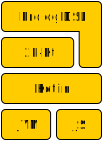
\includegraphics[width=.5\linewidth]{figures/layers}
        \caption{Layered view showing the modules of \twopkt{} and our Kotlin DSL for Prolog}
        \label{fig:layers}
    \end{subfigure}
    \hfill
    \begin{subfigure}{.75\linewidth}
        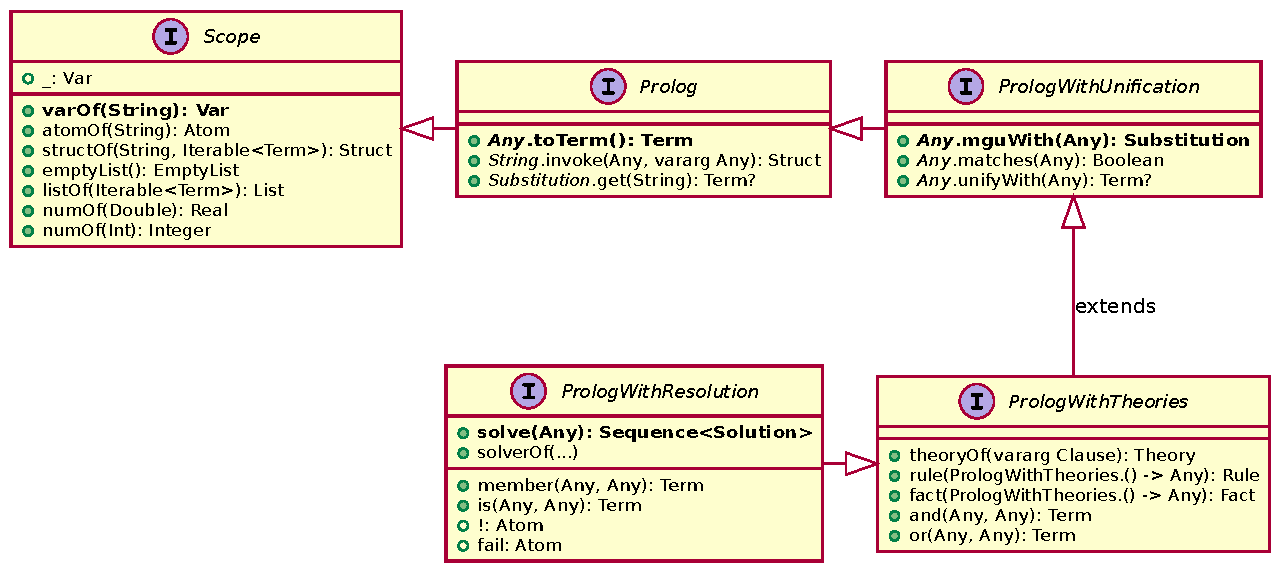
\includegraphics[width=\linewidth]{figures/dsl-types}
        \caption{Structural view showing the API of our Kotlin DSL for Prolog, leveraging on the \twopkt{} API}
        \label{fig:dsl-types}
    \end{subfigure}
    \caption{Architectural view of our Kotlin DSL for Prolog}
\end{figure*}

The Kotlin DSL for Prolog is essentially a compact means to instantiate and use objects from the \twopkt{} library, through a Prolog-like syntax.
%
More precisely, it consists of a small software layer built on top of Kotlin and \twopkt{}, as represented by \cref{fig:layers}.
%
In particular, the DSL is enabled by the five \emph{factory interfaces} depicted in \cref{fig:dsl-types}.
%
We call \emph{factory interface} a type definition whose methods are aimed at \emph{instantiating} objects of related types, as dictated by the Gang of Four' abstract factory pattern \cite{GammaHelmEtAl95}.

The five factory interfaces are: \texttt{Scope}, \texttt{Prolog}, \texttt{Pro\-log\-Wi\-th\-Uni\-fi\-ca\-tion}, \texttt{Pro\-logWi\-thTheo\-ries}, and \texttt{PrologWithResolution}.
%
Each factory type extends the previous one with more LP-related functionalities.
%
So, for instance, while instances of \texttt{Scope} simply provide the basic bricks to create logic terms, instances of \texttt{Prolog} leverage on these bricks to enable the exploitation of the Prolog-like syntax exemplified above.
%
\texttt{PrologWithUnification} extends \texttt{Prolog} with u\-ni\-fi\-ca\-tion-re\-la\-ted facilities, and it is in turn extended by \texttt{Pro\-log\-Wi\-th\-Theo\-ries}, which lets developers create both clauses and theories via a Prolog-like syntax.
%
Finally \texttt{PrologWithResolution} extends \texttt{PrologWi\-thTheories} by adding resolution-related facilities, plus some syntactic shortcuts for writing rules exploiting Prolog standard predicates such as \texttt{member/2}, \texttt{len\-gth/1}, etc.

In the following we provide further details about how each factory contributes to our DSL.

\paragraph{Scope}

The simplest factory type is \texttt{Scope}.
%
As suggested by its name, it is aimed at building terms which must share one or more variables.
%
For this reason, it exposes a number of factory methods -- roughly, one for each sub-type of \texttt{Term} --, some of which are mentioned in \cref{fig:dsl-types}.
%
The main purpose of a scope, however, is to enable the creation of objects reusing the same logic \texttt{Var}iables more than once.
%
Thus, it includes a method -- namely, \kotlin{varOf(String)} -- which always returns the same variable if the same name is provided as input.

For example, to create the term \prolog{member(X, [X | T])}, one may write:
%
\begin{lstlisting}[language=Kotlin]
val m = Scope.empty {
    structOf("member", varOf("X"), consOf(varOf("X"), varOf("T")))
} // m references the term member(X, [X | T])
\end{lstlisting}
%
There, the two calls to \kotlin{varOf("X")} actually return the same object, if occurring within the same scope---whereas they would return different variables if invoked on different scopes.
%
This mechanism is what enables developers to instantiate terms and clauses without having to explicitly refresh variables among different clauses: it is sufficient to create them within different scopes.

\paragraph{Prolog}

The \texttt{Prolog} factory type extends \texttt{Scope} by adding the capability of creating terms through a Prolog-like syntax.
%
To do so, it exposes a number of extension methods aimed at automatically converting Kotlin objects into Prolog terms or using Kotlin objects in place of Prolog terms.
%
The most relevant extension methods are mentioned in \cref{fig:dsl-types}.
%
These methods are:
%
\begin{itemize}
    \item \kotlin{fun Any.toTerm(): Term}, which is an extension method aimed at making any Kotlin object convertible into a Prolog term, through the syntax \kotlin{obj.toTerm()}.
    %
    To convert an object into a term, it leverages on the following type mapping:
    %
    \begin{inlinelist}
        \item a Kotlin number is either converted into a Prolog real or integer number, depending on whether the input number is floating-point or not,
        \item a Kotlin string is either converted into a Prolog variable or atom, depending on whether the input string starts with a capital letter or not,
        \item a Kotlin boolean is always converted into a Prolog atom,
        \item a Kotlin iterable (be it an array, a list, or any other collection) is always converted into a Prolog list, provided that each item can be recursively converted into a term,
        \item a Kotlin object remains unaffected if it is already an instance of \texttt{Term},
        \item an error is raised if the input object cannot be converted into a \texttt{Term}.
    \end{inlinelist}

    \item \kotlin{operator fun String.invoke(vararg Any): Struct},
    %
    which is an extension method aimed at overloading the function invocation operator for strings.
    %
    Its purpose is to enable the construction of compound terms through the syntax \kotlin{"f"}\texttt{(arg$_1$, $\ldots$, arg$_N$)}, which mimics Prolog.
    %
    Its semantics is straightforward: assuming that each \texttt{arg}$_i$ can be converted into a term via the \texttt{Any.toTerm()} extension method above, this method creates a $N$-ary \texttt{Struct}ure whose functor is \kotlin{"f"} and whose $i^{th}$ is \texttt{arg$_i$.toTerm()}.
    %
    So, for instance, the expression
    %
    \begin{center}
        \kotlin{"member"("X", arrayOf(1, true))}
    \end{center}
    %
    creates the Prolog term \prolog{member(X, [1, true])}.

    \item \kotlin{fun Substitution.get(String): Term?}, which is an extension method aimed at overloading the \texttt{get} method of the \texttt{Substitution} type in such a way that is can also accept a string other than a \texttt{Var}iable.
    %
    This enables DSL users to write expressions such as
    \begin{center}
        \kotlin{substitution.get("X")}
    \end{center}
    %
    instead of having to create a variable explicitly via \kotlin{varOf("X")}.
    %
    While we only discuss this method, the main idea here is that every method in the \twopkt{} API accepting some basic Prolog type -- such as \texttt{Var}, \texttt{Atom}, or \texttt{Real} -- as argument should be similarly overloaded to accept the corresponding Kotlin type as well---e.g. \texttt{String} or \texttt{Double}.
    %
    This is what enables a fine-grained integration of our DSL with the Kotlin language and the \twopkt{} library.
\end{itemize}
%
It is worth highlighting that every \texttt{Prolog} object is also a particular sort of \texttt{Scope}.
%
So, converting the same string into a \texttt{Var}iable twice or more times, within the same \texttt{Prolog} object, always yields the exact same variable.

\paragraph{Prolog with unification}

The \texttt{Pro\-logWi\-thU\-ni\-fi\-ca\-tion} factory type extends \texttt{Prolog} by adding the capability of
%
\begin{inlinelist}
    \item computing the most general unifier (MGU) among two terms,
    \item checking whether two terms match or not according to logic unification -- i.e., checking if a MGU exists unifying the two terms --, and
    \item computing the term attained by unifying two terms---assuming an MGU exists for them.
\end{inlinelist}
%
To do so, it exposes a number of extension methods aimed at providing unification-related support to Kotlin objects, provided that they can be converted into terms.
%
The most relevant extension methods are mentioned in \cref{fig:dsl-types}.

\paragraph{Prolog with theories}

The \texttt{Pro\-logWi\-thTheo\-ries} factory type extends \texttt{Pro\-logWi\-thU\-ni\-fi\-ca\-tion} by adding the capability of creating logic clauses (e.g. rules and facts) and theories.
%
To do so, it exposes a number of methods aimed supporting the conversion of Kotlin objects into Prolog clauses -- through the syntactic facilities presented so far --, and their combination into theories.
%
The most relevant methods, mentioned in \cref{fig:dsl-types}, are the following:
%
\begin{itemize}
    \item \kotlin{fun theoryOf(vararg Clause): Theory}, an ordinary method aimed at creating a logic \texttt{Theory} out of a variable amount of clauses.

    \item \kotlin{infix fun Any.`if`(Any): Rule}, which is an extension method aimed at creating logic rules via a Prolog-like syntax in the form \kotlin{head `if` body}.
    %
    Its semantics is straightforward: assuming that both \kotlin{head} and \kotlin{body} can be converted into logic goals via the \kotlin{Any.toTerm()} extension method above, this method creates a binary \texttt{Struct}ure whose functor is \texttt{`:-'} and whose arguments are \kotlin{head.toTerm()} and \kotlin{body.toTerm()}.
    %
    Similar methods exists -- namely, \kotlin{and}, \kotlin{or}, etc. --  to create conjunctions or disjunctions of clauses.
    %
    \item \kotlin{fun rule(PrologWithTheories.() -> Any): Rule}, an ordinary method aimed at creating a rule in a separate scope, thus avoiding the risk of accidentally referencing the variables created elsewhere.
    %
    It creates a fresh, empty, and nested instance of \texttt{Pro\-logWi\-thTheo\-ries} and accepts a function with receiver to be invoked on that nested instance.
    %
    The function is expected to return a Kotlin object which can be converted into a Prolog rule.
    %
    Any variable possibly created within the nested scope is guaranteed to be different than any homonymous variable defined elsewhere.
    %
    \item \kotlin{fun fact(PrologWithTheories.() -> Any): Fact},  analogous to the previous method, except that it is aimed at creating Prolog facts.
    %
    So, for instance, one may write
    %
\begin{lstlisting}[language=Kotlin]
val r1 = fact {
    "member"("X", consOf("X", `_`))
}
val r2 = rule {
    "member"("X", consOf(`_`, "T")) `if` "member"("X", "T")
}
\end{lstlisting}
    %
    while being sure that the \texttt{X} variable used in \texttt{r1} is different than the one used in \texttt{r2}.
    %
\end{itemize}

\paragraph{Prolog with resolution}

The \texttt{Pro\-logWi\-thRe\-so\-lu\-tion} factory type extends \texttt{Pro\-logWi\-thU\-ni\-fi\-ca\-tion} by adding the capability of performing logic queries and consuming their solutions attained through the standard Prolog semantics.
%
To do so, it exposes a number of methods aimed at supporting
%
\begin{inlinelist}
    \item the instantiation of Prolog \texttt{Solver}s,
    \item the loading of Prolog theories, either as static or dynamic knowledge bases (KB), and
    \item the invocation of Prolog queries on those KB.
\end{inlinelist}
%
The most relevant methods, mentioned in \cref{fig:dsl-types}, are the following:
%
\begin{itemize}
    \item \kotlin{fun solve(Any, Long): Sequence<Solution>},
    which is an ordinary method aimed at executing Prolog queries without requiring a new solver to be explicitly created.
    %
    It accept a Kotlin object as argument -- which must be convertible into a Prolog query --, and an optional timeout limiting the total amount of time the solver may exploit to compute a solution.
    %
    If the provided arguments are well formed, this method returns a \texttt{Sequence} of \texttt{Solution}s which \emph{lazily} enumerates all the possible answers to the query provided as input, using Prolog's SLDNF proof procedure.

    \item \kotlin{fun staticKb(vararg Clause)}, which is an ordinary method aimed at loading the \emph{static} KB the \texttt{solve} method above will operate upon.

    \item \kotlin{fun dynamicKb(vararg Clause)}, which is analogous to the previous method, except that it loads the \emph{dynamic} KB the \texttt{solve} method above will operate upon.

    \item \kotlin{fun member(Any, Any): Struct} which is an ordinary method aimed at easily creating invocations of the \prolog{member/2} built-in predicate.
    %
    While we only discuss this method, the main idea here is that every standard built-in predicate in Prolog has a Kotlin counterpart in \texttt{Pro\-logWi\-thRe\-so\-lu\-tion} accepting the proper amount or arguments and returning an invocation to that built-in predicate.
    %
    This is aimed easing the exploitation of the standard Prolog predicates to developers leveraging our DSL.
    %
    So, for instance, we also provide facility methods for built-in such as \prolog{is/2}, \prolog{+/2}, \prolog{-/2}, \prolog{!/0}, \prolog{fail/0}, \prolog{append/3}, etc.
\end{itemize}
%
Instances of \texttt{Pro\-logWi\-thRe\-so\-lu\-tion} are created and used via the
%
\begin{center}
        \kotlin{fun <R> prolog(PrologWithResolution.() -> R): R}
\end{center}
%
static method, which accepts a lambda expression letting the user exploit the DSL on the fly, and returns the object created by this lambda expression.
%
This is for instance what enables developers to write the code snippet discussed in \cref{ssec:dsl-overview}.

\section{Case study: N-Queens}\label{sec:case-study}

We present now a brief example demonstrating how, by integrating multiple programming paradigms, developers may easily produce compact and effective solutions.
%
Suppose one is willing to implement the following Kotlin method
%
\begin{center}
    \kotlin{fun nQueens(n: Int): Sequence<List<Position>>}
\end{center}
%
aimed at computing all the possible solutions to the N-Queens problem.
%
More precisely, the method is expected to enumerate all the possible dispositions of $n$ queens on a $n \times n$ chessboard, such that no queen can be attacked by others.
%
Each solution can be represented by a list of queen positions, in the form $[(1, Y_1),\ \ldots,\ (n, Y_n)]$, where each $Y_i$ represent the row occupied by the $i^{th}$ queen---i.e., the one in column $i$.

Computing all solutions for the N-Queens problem may require a lot of code in most programming paradigms.
%
However, in LP, the solution is straightforward and compact.
%
One may, for instance, leverage the Prolog code depicted in \cref{lst:nqueens-prolog}.
%
\lstinputlisting[
    float,
    language=Prolog,
    caption={Logic theory aimed at computing solutions for the N-Queens problem},
    label={lst:nqueens-prolog},
]{listings/nqueens.pl}
%
which can satisfy queries in the form
%
\begin{center}
    \prolog{?- solution(N, [(1, Y1), ..., (N, YN)])}
\end{center}
%
(provided that some actual $N$ is given) by instantiating each variable \texttt{Yi}.

Thanks to our Kotlin DSL for Prolog, one may exploit the elegance of LP in implementing the aforementioned \texttt{nQueens} method.
%
For instance, one may implement it as shown in \cref{lst:nqueens-kotlin}.
%
\lstinputlisting[
    float,
    language=Kotlin,
    caption={Kotlin code aimed generating the theory depicted in \cref{lst:nqueens-prolog}},
    label={lst:nqueens-kotlin},
]{listings/NQueens.kt}
%
This implementation produces a \emph{lazy} stream of solutions to the N-Queens problem, given a particular value of $n$.
%
In doing so, it takes advantages not only of logic- but also of functional-programming paradigm.
%
For instance, on the last line, it exploits the \texttt{map} high-order function to build a list in the form $[(1, Y_1),\ \ldots,$ $(n, Y_n)]$, to be provided as argument of \prolog{solution/2}.

A number of minuti\ae{} may be noted as well by comparing the Prolog code with its Kotlin counterpart.
%
For instance, Prolog operators (such as \texttt{=$\backslash$=/2}, \prolog{-/2}, etc.) retain their infix notations in the Prolog DSL.
%
This is possible because they are part of the DSL, in the same way as Prolog built-in predicates (such as \prolog{between/3}).
%
This implies the Kotlin compiler can prevent standard operators and built-in from being silently mistyped.

\section{Recap and Research Perspectives}\label{sec:conclusions}

In this chapter we propose a novel way of integrating the logic, object-oriented, functional, and imperative programming paradigms into a single language, namely Kotlin.
%
More precisely, we describe how a domain-specific language (DSL) for Prolog can be built on top of the Kotlin language by exploiting the \twopkt{} library.
%
The proposed solution extends the Kotlin language with LP facilities by only relying on its own mechanisms -- therefore no external tool is necessary apart from Kotlin itself and \twopkt{} --, even if, however, analogous extensions can in principle be constructed for other high-level languages as well---such as Scala.

Our DSL is currently implemented as part of the \twopkt{} project -- namely, within the \texttt{dsl-*} modules --, and it is hosted on both GitHub \cite{homepage2PKt} and Maven Central.
%
Other than being available to the public for general purpose usage -- under the terms of the Apache License 2.0\footnote{\url{https://www.apache.org/licenses/LICENSE-2.0}} open-source license --, the DSL is currently extensively exploited to implement the unit tests of \twopkt{} itself.

While in this chapter we discuss the design rationale and architecture of our DSL by explicitly focusing on Kotlin as our target technology, in the future we plan to generalise our approach, possibly tending to technology independence.
%
Furthermore, we plan to provide other implementations of our DSL, targeting other high-level languages and platforms, in order to make logic programming and its valuable features available in general-purpose programming languages and frameworks.

As concerns possible research directions and applications, in the future, we plan to exploit our DSL in several contexts.
%
For instance, we argue our DSL may ease the usage of the logic tuple spaces offered by the \tusow{} technology \cite{tusow-icccn2019}.
%
Similarly, we believe our DSL may be used as a basic brick in the creation of logic-based technologies for MAS, as the MAS community is eager of general-purpose, logic-based technologies targetting the JVM platform \cite{lptech4mas-jaamas35}.
%
Along this line, we argue logic-based languages for MAS may benefit from the integration of our DSL -- or a similar one -- to support the reasoning capabilities of agents.
%
Finally, we plan to exploit our DSL within the scope of XAI \cite{xaisurvey-ia14}, to ease the creation of hybrid (i.e., logic + machine-learning) systems, and management on the symbolic side.


\chapter{Bridging LP and Machine Learning}
\label{chap:mllib}

\mystudentsthesis{Master's}{Castiglio2021}

Symbolic and sub-symbolic AI are complementary under a number of perspectives.
%
The same is true for their major techniques, namely logic programming (LP) and neural networks (NN).
%
For this reason, many recent contributions from the literature are discussing the possible frameworks for their integration and hybridisation.

However, what is currently slowing down scientific progress in this context is not the lack of ideas concerning \emph{how} such integration and hybridisation may occur.
%
Rather, we believe the bottleneck is caused by the lack of suitable technologies enabling and easing the experimentation of integrated or hybrid systems.
%
Logic-based technologies are in fact technological islands, for which poor care is given to the construction of bridges with the rest of the AI land.

Accordingly, in this chapter, we address the issue of supporting machine learning (ML) -- and, in particular, neural-networks-based training and inference -- in logic programming.
%
In doing so, we follow the twofold purpose of
%
\begin{enumerate}
    \item letting logic programmers exploit the benefits of sub-symbolic AI, and, in particular, neural networks; and
    \item enabling the experimentation of hybrid systems -- involving both logic and neural processing of data -- in practice.
\end{enumerate}


More precisely, we discuss the design and prototyping of a logic based API for machine learning.
%
Such API consists of a set of logic predicates enabling the representation, training, testing, and exploitation of sub-symbolic predictors in LP---possibly, out of data expressed in logic form.
%
In other words, our API lets logic programmers use neural networks in their programs -- e.g. to train or exploit classifiers or regressors --, without requiring them to abandon the logic realm.
%
Of course, to make this possible, our API supports the whole gamma of low level tasks which are commonly involved in a ML workflow---including, but not limited to, data preprocessing, cross-validation, etc.

Technically, we prototype our API via a logic library -- namely, the \mllib{} -- targetting the \twopkt{} ecosystem, and the JVM platform.
%
It consists of a number of primitives bridging the logic realm with some underlying machine-learning library, allowing Prolog to manipulate sub-symbolic facilities such as datasets, neurons, layers, or activation functions, and vice versa.
%
\deeplearningforj{} is the underlying library we leverage upon in this chapter---selected after meticulous technological analysis (here reported as well).
%
However, our design is general enough to support other libraries and, possibly, different platforms---e.g. Tensorflow over Python.

In perspective, we argue that our work represents the first step towards a wider degree of interoperability among logic- and sub-symbolic AI.
%
In fact, one the long run, we aim to enable the design and construction of hybrid systems, fruitfully and dynamically combining the major advantages of both approaches to artificial intelligence by mixing inferential (via logic programming) and intuitive (via neural networks) reasoning capabilities.
%
Along this path, the proposed API is one key enabling factor, as it supports the creation of logic-based inferential engines which are capable of learning from data via state-of-the-art mechanisms.
%
Dually, by supporting the training of neural networks from logic data, our API can also be considered as a tool for endowing sub-symbolic predictors with prior, high-level knowledge.

Accordingly, the reminder of this chapter is organised as follows.
%
In \cref{sec:requirements}, we describe and analyse the supervised ML domain, with the purpose of identifying which functionalities our logic API for ML should support, and how exactly they are expected to work.
%
Then, in \cref{sec:project}, we delve into the design of the \mllib{} discussing and motivating conventions, syntactic choices, and architectural decisions.
%
In \cref{sec:tech}, we then discuss a number of technology- and platform-related aspects arising when prototyping the \mllib{}.
%
There, we motivate technological commitments such as \twopkt{} and \deeplearningforj{}.
%
\Cref{sec:examples} is where we discuss a number of examples concerning the usage of the \mllib{}, and its potential applications.
%
Finally, \cref{sec:conclusions3} concludes the chapter, providing some insights about the future research directions stemming from this work.


\section{Logic API for ML: Requirements, Analysis, and Modelling}
\label{sec:requirements}

\subsection{Goals}\label{ssec:goals}

Broadly speaking, a logic API for ML enables the combination or integration of symbolic AI's expressiveness and sub-symbolic AI's flexibility, at a deeper and unprecedented level.
%
Here we describe a number of motivating features, which we choose to pursue as goals.


\paragraph{Declarative machine learning}

Declarative ML is a paradigm by which data scientists' code should only specify \emph{what} a ML workflow should do, by leaving the underlying platform in charge to understand \emph{how}.
%
This is partially supported by the current practice of data science which relies on high-level languages (like Python) and libraries of elementary components to be composed (e.g. Scikit-Learn).
%
However, the solutions proposed so far do not leverage upon inherently declarative frameworks like LP, but rather on object oriented languages---which eventually need imperative statements to be provided by data scientists.
%
An API for ML should then be designed to support the declarative expression of all possible aspects of a ML workflow in the LP framework.
%
This would be useful under both a logic and ML perspective.
%
In fact, it would pave the way towards the exploitation of ML within the LP community, other than providing data scientists with a way to describe their ML workflows in a formal and runnable way.


\paragraph{Symbolic data sources}

Logic knowledge bases are a peculiar way of collecting knowledge.
%
Unlike datasets and DBMS, they represent information in symbolic form, via -- possibly \emph{intensional} -- logic formul\ae{}.
%
Hence, they can virtually represent any sort of datum -- be it atomic, compound or structured -- via a concise (yet very expressive) language, while possibly saving space.
%
Accordingly, when combining LP with ML, knowledge bases should be exploitable as data sources as well---other than ordinary CSV files or relational databases.

\paragraph{Hybrid reasoning}

Automatic reasoning may greatly benefit from sub-symbolic AI to overcome its inherent crispness.
%
Fuzzy data could then be suitably and coherently processed by a sub-symbolic predictor as part of a wider symbolic resolution process.
%
To make this possible, sub-symbolic predictors should be representable, trainable, and queryable as any other logic predicate, without requiring the semantics of logic resolution to be affected.
%
Consequently, logic programs should be endowed with ad-hoc predicates and syntactical categories, aimed at representing and manipulating sub-symbolic predictors and data.

\paragraph{Model selection via resolution}

Logic resolution essentially consist of a search procedure aimed at finding solutions in a proof tree.
%
This could be applied to a common step of any ML workflow---namely \emph{model selection}.
%
There, data scientists must assess several predictor families, to select the one which is better suited for the learning task at hand.
%
Then, they must search for the best hyper-parameters for the selected family of predictors.
%
All such choices involve several sorts of predictors, with possibly different hyper-parameters, to be trained and compared---either in an orderly fashion or in parallel.
%
LP naturally captures the non-deterministic exploration of a space of possible choices.
%
Hence it is well suited to both declaratively represent and implement model selection.

\subsection{Domain Description}\label{ssec:analysis}

To support the aforementioned goals,
our logic API must cover the full gamma of tasks involved in any possible ML workflow.

Briefly speaking, a ML workflow is the process of producing a suitable predictor for the available data and the learning task at hand, following the purpose of later exploiting that predictor to draw analyses or to drive decisions.
%
Hence, any ML workflow is commonly described as composed by two major phases, namely training -- where predictors are fit on data -- and inference---where predictors are exploited.
%
However, in practice, further phases are included, such as data provisioning and preprocessing, as well as model selection and assessment.

In other words, before using a neural network in a real-world scenario, data scientists must ensure it has been sufficiently trained and its predictive performance is sufficiently high.
%
In turn, training requires
%
\begin{inlinelist}
    \item an adequate amount of data to be available,
    \item the structure of the network under training to be defined, and
    \item any other hyper-parameter (e.g. learning rate, momentum, batch size, epoch limit, etc.) to be fixed.
\end{inlinelist}
%
Data must therefore be provisioned before training, and, possibly, pre-processed to ease training it self---e.g. by normalising data or by encoding non-numeric features into numeric form.
%
The structure of the network must be defined in terms of (roughly) input, hidden, and output layers, as well as their activation functions.
%
Finally, hyper parameters must be carefully tuned according to the data scientist's experience, and the time constraints and computational resources at hand.
%
\begin{figure}
    \centering
    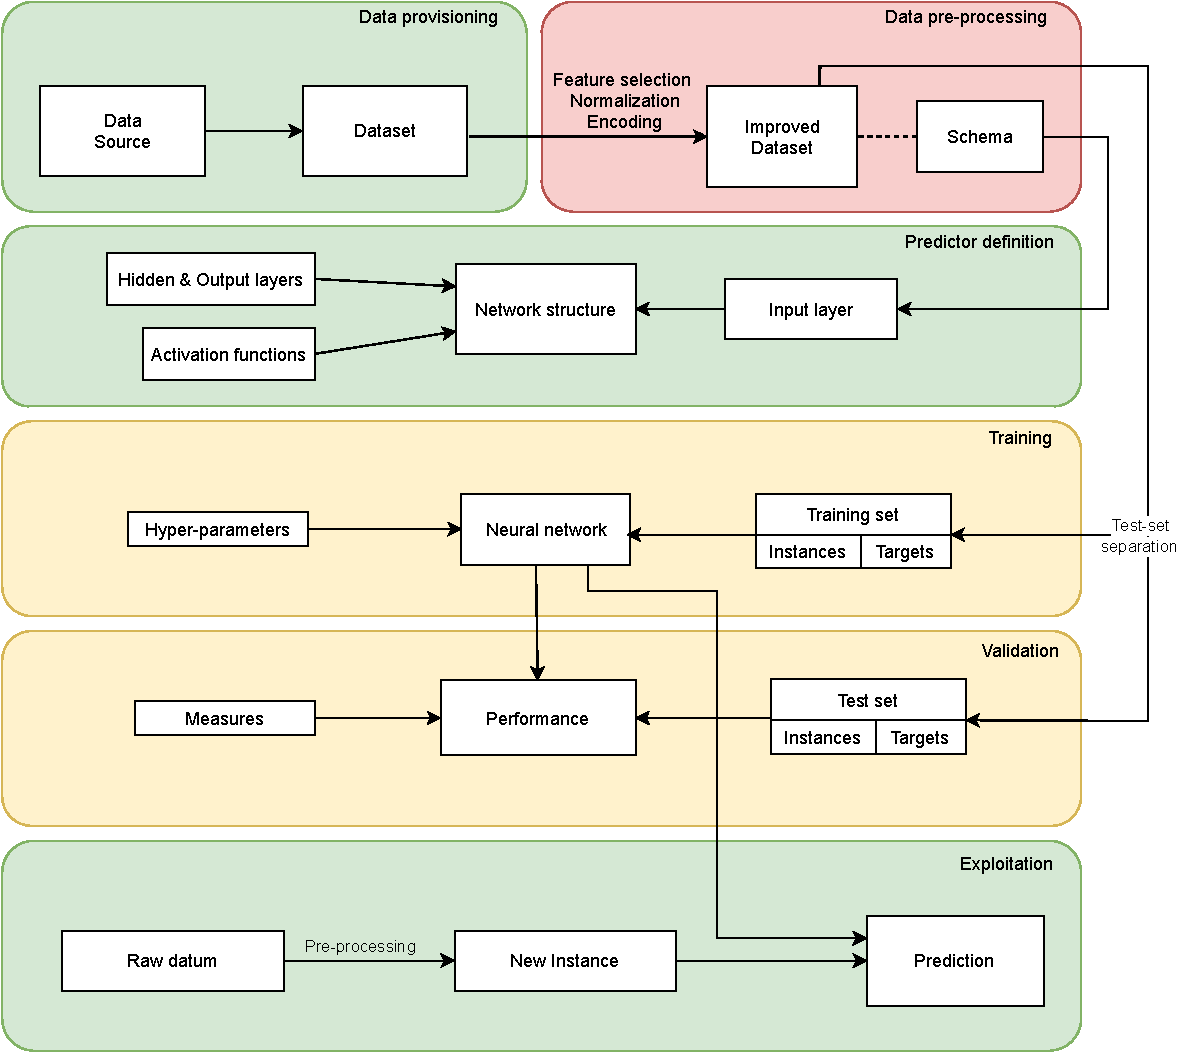
\includegraphics[width=\linewidth]{figures/phases1.pdf}
    \caption{Major phases of the generic ML workflow}
    \label{fig:activities1}
\end{figure}

Thus, from a coarse-grained perspective, a machine learning workflow can be conceived as composed by six major phases, overviewed in \cref{fig:activities1} and described into the following paragraphs.
%
The background colour of each phase denotes the expected design and implementation effort for supporting that phase in our logic API for ML (low effort $\leftrightarrow$ green, moderate effort $\leftrightarrow$ yellow, considerable effort $\leftrightarrow$ red).

\paragraph{Dataset loading}

Provided that the data provisioning phase has resulted into a dataset -- roughly, a collection of homogenous data, often coming in the form of a single file, a folder or a database --, the first step of any ML workflow consists of loading that dataset in memory for later processing.
%
To support such step, ML frameworks come with ad-hoc functionalities aimed at loading the dataset by reading a file from the local file system, by fetching it from the Web, or by querying a DBMS.
%
These usually come in the form of either classes or functions, coherently w.r.t. the object-oriented nature of mainstream ML frameworks.

Our logic API for ML should expose ad-hoc \emph{predicates} to serve the same purposes.
%
Furthermore, however, it should also support the loading of datasets out of logic theories of facts and rules.

\paragraph{Data pre-processing}

Raw datasets are often inadequate to favour predictors' training.
%
Hence, dataset pre-processing is commonly practised to increase the effectiveness of any subsequent training phase.
%
Pre-processing, in practice, involves a number of bulk operations to be applied to the whole dataset, following several purposes, such as:
%
\begin{inlinelist}
    \item homogenize the variation ranges of the many features sampled by the dataset,
    \item detect irrelevant features and remove them,
    \item construct relevant features by combining the existing ones,
    \item encoding non-numeric features into numeric form, and
    \item\label{preprocessing:partitioning} horizontal (by row) or vertical (by column) partitioning of the dataset.
\end{inlinelist}
%
Purpose \ref{preprocessing:partitioning}, in particular, is of paramount importance, as it supports the \emph{test set separation} -- that is, a fundamental step to be performed at the very beginning of any correct ML workflow, to later enable validation and testing --, as well as splitting input-related columns from output-related ones---which, in turn, is fundamental to support training.

Notably, our logic API for ML should support all such purposes, via a concise (yet expressive) predicates letting the logic data-scientist decide which pre-processing operations to perform, and when.
%
In practice, this involves a number of predicates supporting bulk manipulations to be applied to the whole dataset, such as computing statistical moments (e.g. mean, variance, standard deviation, etc.), or aggregated measures (e.g. min, max, etc.) on a column-wise basis, as well as transforming (e.g. transforming a categorical feature in numeric form via the one-hot encoding).


\paragraph{Predictor selection and definition}

Many sorts of predictors could be used in principle to perform supervised learning---e.g. neural networks, decision trees, support vector machines, etc.
%
Unless some technical or administrative constraint exists, it is a common practice for data scientists to spend some time selecting the most adequate sort of predictor for the data and the learning task at hand.
%
This is a common phase in virtually any ML workflow.
%
Once a particular sort of predictor has been chosen, data scientists need a way to specify the shape the to-be-trained predictor should have.
%
Of course, such specification should take into account the schema of the input data, as well as the schema of the expected outcomes to be produced by the predictor.
%
The are however other aspects to be tuned, generally referred to as \emph{hyper-parameters}.

Consider the case of neural networks as an example.
%
Decision points in this case concern the choice of
%
\begin{inlinelist}
    \item which and how many hidden layers (of neurons) to adopt,
    \item how to interconnect them, and
    \item which activation functions to adopt for the neurons therein contained.
\end{inlinelist}

Accordingly, our logic API for ML should support the specification of as many sorts of predictors as possible, as well as their parametrisation.
%
Once again, predicates should be defined to serve this purpose.
%
In particular, at least one ad-hoc predicate should be defined for each sort of predictor to be supported, carrying as many arguments as the possible hyper-parameters that could be specified for that sort of predictors.
%
In case hyper-parameters cannot conveniently represented as raw logic types (numbers or strings), ad-hoc predicates should be provided as well for constructing structured hyper-parameters values.

In the particular case of neural networks, ad-hoc predicates should be provided to construct layers, and activation functions, and to combine them to create arbitrarily complex network architectures.

\paragraph{Training}

Predictors' training plays a pivotal role in ML workflows.
%
This is the phase where predictors are fit on the available data or, in other words, automated learning actually occurs.
%
Generally speaking, training can be modelled in LP as single predicate, mapping untrained predictors into trained ones, possibly via a number of learning parameters (e.g. learning rate or momentum for NN, or maximum depth for DT), or stopping criteria (e.g. max epochs for NN, or max depth for DT), other than, of course, the data to be used for training.
%
Once again, several ad-hoc predicates should be defined to support structured parameters or stopping criteria in our logic API for ML.
%
Furthermore, regardless of its shape, the training predicate should accept some arguments aimed at specifying whether the columns of the training set should be considered as inputs or outputs.

\paragraph{Exploitation}

Exploitation is commonly the last phase of any ML workflow.
%
Here, trained predictors are used to draw predictions on new data---i.e. different data w.r.t. the one used for training.
%
In particular, given a raw datum having the same schema of the input data used for training -- there including any prior pre-processing phase --, the trained predictor can be exploited to compute the corresponding prediction---even if (and especially because) the raw datum has never been observed before by that predictor.
%
In most common cases, predictions attempt to solve classification or regression problems.
%
In any case, yet another general predicate should be added to our logic API for ML to support drawing predictions out of a trained predictor and a set of raw data (or a single datum).
%
Ad-hoc predicates may be provided as well to explicitly model higher-level tasks, such as classification and regression.
%
Finally, it should be possible to store, retrieve, and re-apply any pre-processing procedure possibly defined before training, to the raw data for which predictions should be drawn---in order to make it acceptable for the predictor as an input.

\paragraph{Validation}

Validation is the \emph{penultimate} step of any ML workflow: it succeeds training and precedes exploitation.
%
It is here discussed as last because it technically relies on the capability of drawing predictions via trained predictors---which is treated in the paragraph above.

Generally speaking, validation attempts to measure the predictive performance of a trained predictor, with the purpose of assessing if and to what extent it will generalise to new, unseen data.
%
To do so, the predictor is tested against the test set---that is, a collection of unseen data, for each expected predictions exist.
%
The discrepancy (or similarity) among the actual and expected predictions is then measured via ad-hoc scoring functions (a.k.a. measures), resulting in a performance assessment for the trained predictor.
%
Many measures may be used to assess classifiers (e.g. accuracy, F1-score, etc.) and as many to assess regressors (e.g. MAE, MSE, R$^2$, etc.).
%
Hence, to support validation, our logic API for ML should provide predicates to compute each possible measure.

\subsection{Analysis and Modelling}
\label{ssec:modelling}

Here we analyse the ML domain w.r.t. our goals, and we elicit the most relevant entities and actions our logic API should support.
%
In other words, we derive the meta-model leading the design, implementation, and usage of our logic API for ML.

There are five major sorts of entities by which any ML workflow can be described.
%
These are introduced below:
%
\begin{description}
    \item[Value:] a scalar, vectorial, matrix, or tensorial datum from a given domain (e.g. an integer or real number, or a vectors of integer or real numbers, as well as a string, a table, a time series, etc.).

    \item[Schema:] a concise and formal description of a domain (i.e. a set of values).
    %
    For scalar values, schemas are essentially data types (e.g. integers, reals, strings, etc.), while for non-scalar data they carry information about the name, index, and type of each single scalar component.

    \item[Dataset:] a collection of values matching a particular schema---which is supposed to be known.

    \item[Transformation:] any operation aimed at transforming an entity dataset into another other---commonly, a dataset into either another dataset (e.g. normalization, standardization, etc.) or a value (e.g. max, min, average, etc.)
    %
    From an algebraic perspective, it is a function.
    %
    From a computational perspective it is an algorithm.

    \item[Predictor:] a stateful computational entity capable of
    %
    \begin{inlinelist}
        \item drawing predictions (i.e. outputting values) out of (possibly unseen) input values, according to its internal state
        \item updating its internal state according to a dataset (to improve future predictions)
    \end{inlinelist}
\end{description}

\begin{figure}
    \centering
    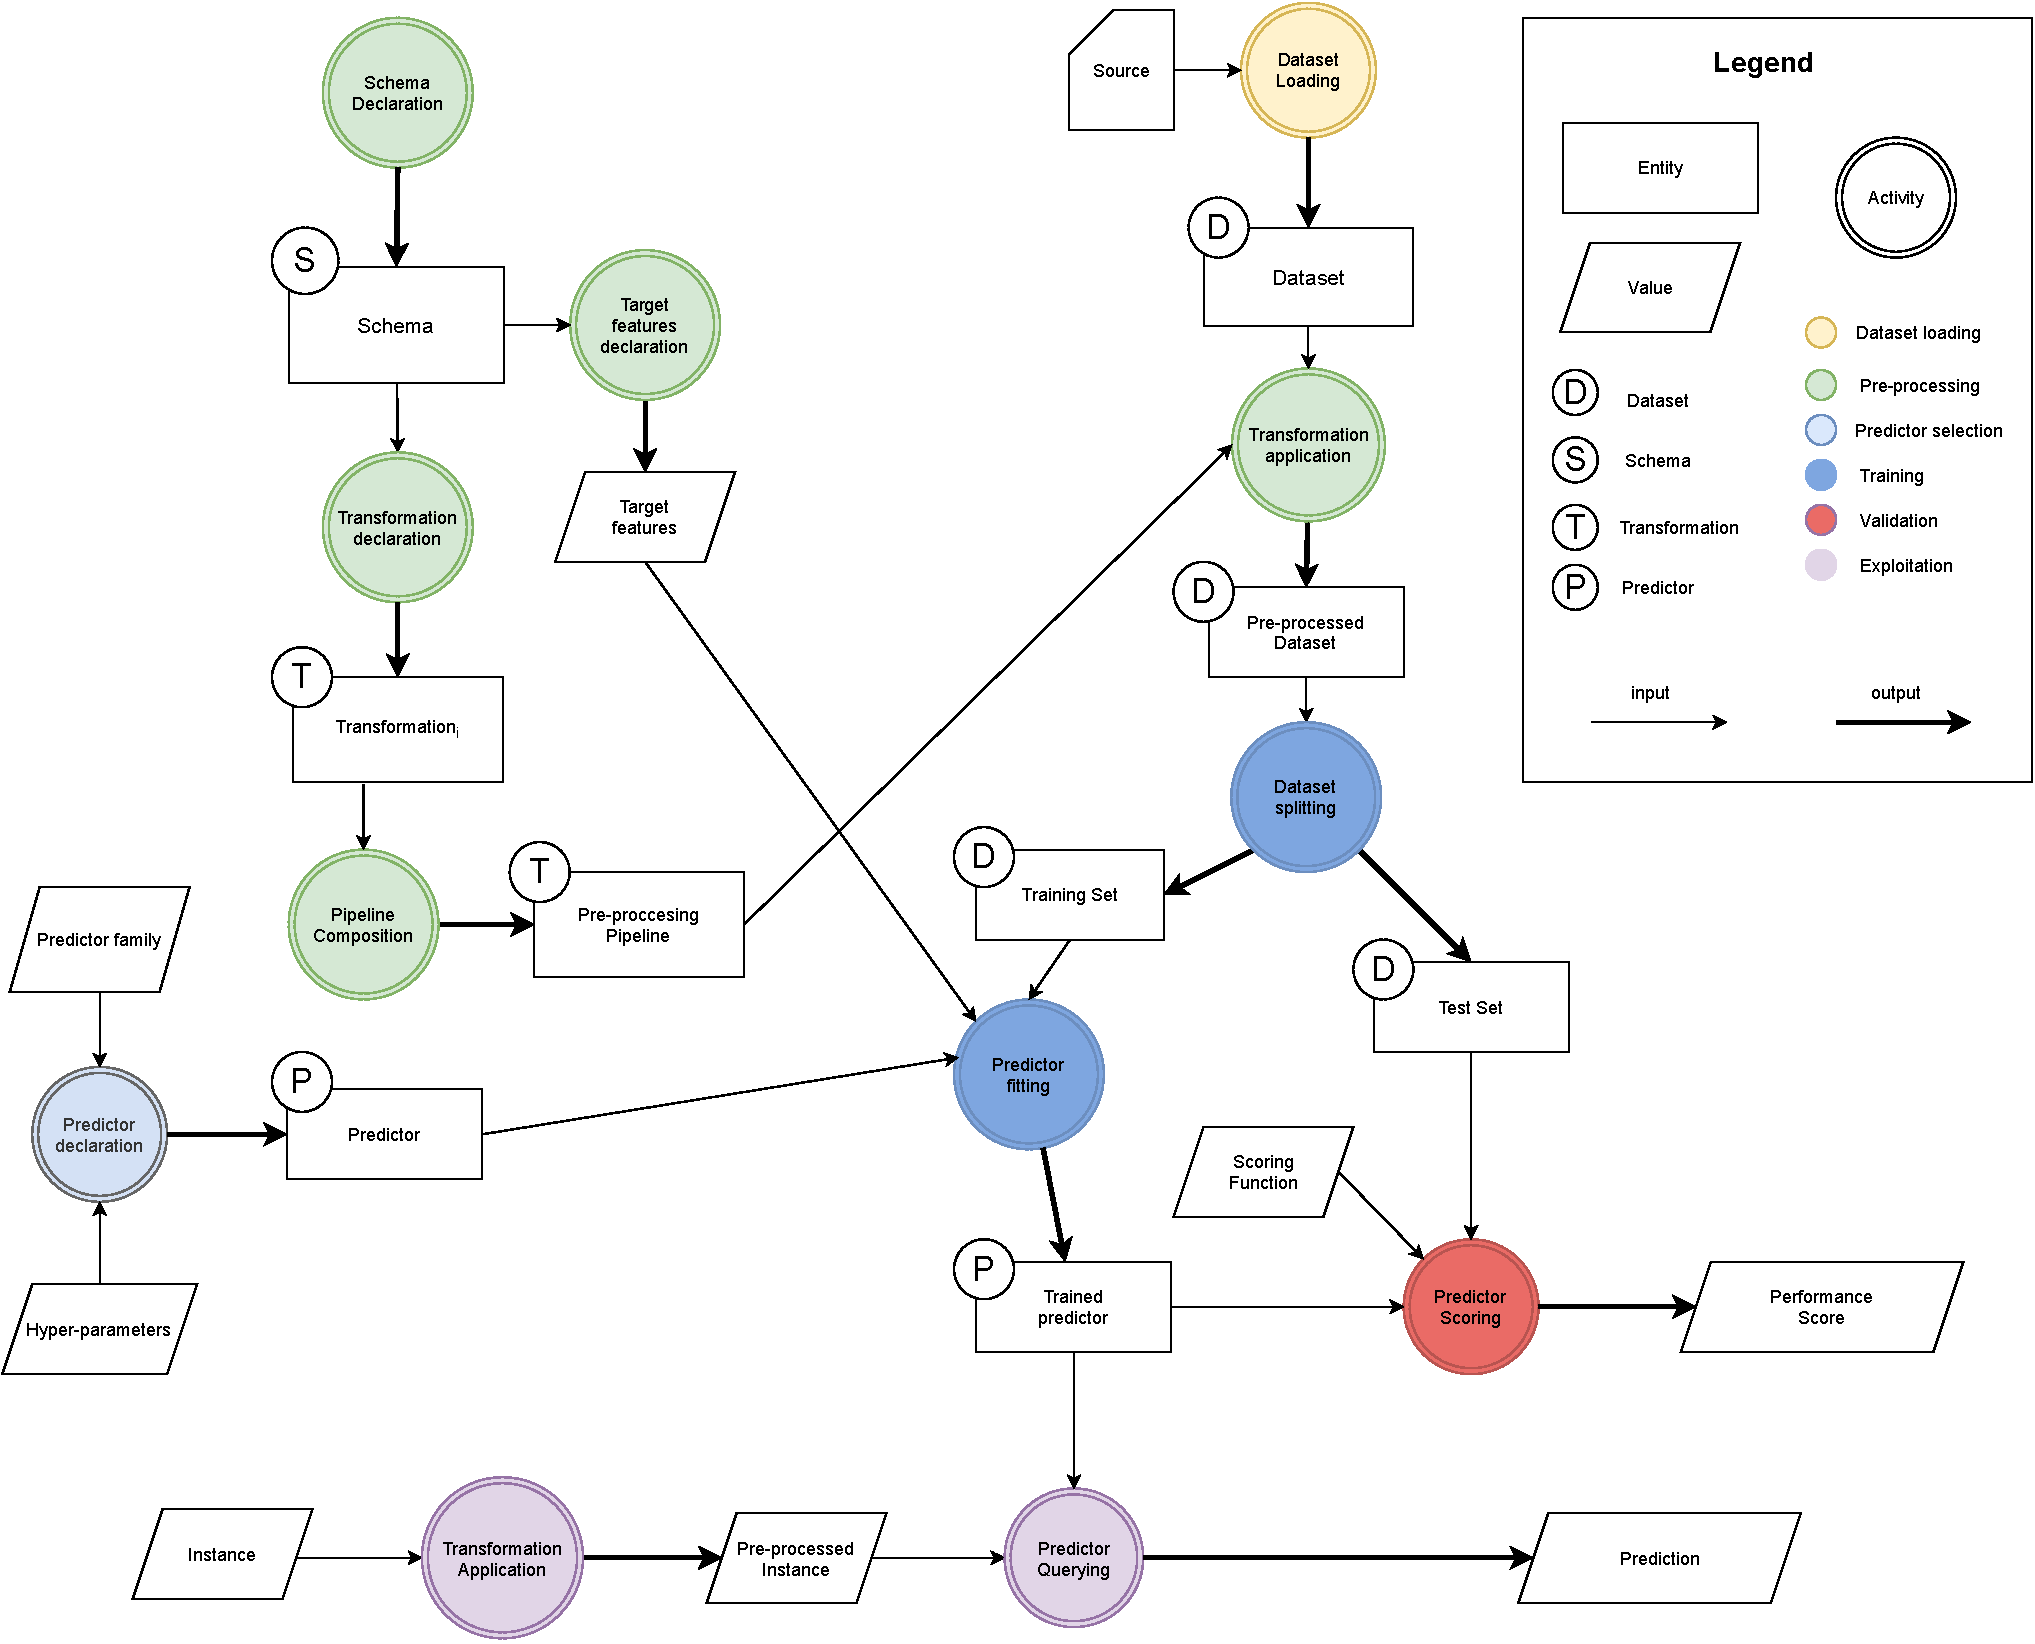
\includegraphics[width=\linewidth]{figures/phases2.pdf}
    \caption{Model and meta-model of a logic API for ML}
    \label{fig:fasi2}
\end{figure}

Our logic API for ML supports the representation, combination, and manipulation of entities of these kinds.
%
In particular, \cref{fig:fasi2} depicts the overall workflow, the specific activities therein contained, and the involved entities, from the user perspective.
%
Each phase of a ML workflow is characterised by a specific set of activities the data scientist may be willing to perform.
%
These should be therefore declaratively representable in logic.

Accordingly, in the reminder of this section, we enumerate the most relevant activities our logic API should support, and the entities they operate upon.
%
Notably, activities are grouped w.r.t. the ML phases they operate in, according to the ML workflow elicited in \cref{ssec:analysis}.

For instance, the following activities make sense into the \emph{dataset loading} phase as their major purpose it to support the loading of a dataset into a solver's memory, and its preparation for sub-sequent processing:
%
\begin{description}
    \item[Dataset loading] | i.e. the operation of loading a dataset from either a value -- representing either a local or remote file --, or from a Prolog theory
    \item[Schema declaration] | i.e. the operation of constructing a representation for a given schema
    \item[Target features declaration] | i.e. the operation of tagging a portion of features of some schema as either inputs or outputs (a.k.a. targets)
    \item[Dataset splitting] | i.e. the operation of horizontally partitioning a dataset into two or more smaller datasets
\end{description}

Subsequently, data scientists will commonly enter the \emph{dataset pre-processing} phase.
%
Here, they may be willing to define transformations or cascades of transformations (pipelines, henceforth) to be eventually applied on datasets:
%
\begin{description}
    \item[Transformation declaration] | i.e. the operation of declaratively encoding a transformation operation to be applied to all data in a dataset
    Such kinds of transformations can be modelled as functions accepting a dataset as input and producing a dataset as output
    \item[Pipeline composition] | i.e. the operation of declaratively constructing a composite transformation as a cascade of simpler transformations
    \item[Transfornmation application] to a dataset | i.e. the operation of actually constructing a new dataset from a prior dataset and a transformation
\end{description}

The next phase commonly involves the \emph{definition} of one or more predictors via a unique meta-activity, namely:
%
\begin{description}
    \item[Predictor declaration] | i.e. the operation of constructing a representation for a particular predictor, which implies choosing the predictor family and specifying actual values for its hyper parameters
\end{description}
%
Of course, as many families of predictors exist, and each one is characterised by its own set of formal hyper-parameters, many variant if this operation may eventually be defined in practice.

Eventually, declared predictors may enter the \emph{training} phase, meaning that their learning from data should be triggered.
%
This can be achieved via yet another activity, namely:
%
\begin{description}
    \item[Predictor fitting] w.r.t. a training set of data | i.e. the operation of fitting a predictors' internal parameter on some provided training data
\end{description}
%
Again, given the variety of predictors available, this operation may come with several predictor specific variants accepting different learning parameters.

Once in their \emph{inference} phase, trained predictors may eventually be exploited to be draw predictions.
%
Hence, this is yet another relevant activity, namely:
%
\begin{description}
    \item[Predictor querying] | i.e. the operation where (possibly unseen) values are provided to some trained predictor as a query, and the resulting values are interpreted as predictions
\end{description}

Finally, in the \emph{validation} phase, trained predictors should be assessed by measuring their performance w.r.t. some test data
%
This is yet another meta-activity, with several possible variants depending on the particular measure being exploited:
%
\begin{description}
    \item[Predictor scoring] | i.e. the operation of computing a scoring value out of a trained predictor, a test dataset, and a scoring function
\end{description}

%
\Cref{fig:fasi2} provides an overview of the overall workflow these activities are involved into.
%
In particular, it represents inter-dependencies among all such activities, other than stressing what sorts of entities they accept as input and produce as output.
%
In the next section, we discuss how these activities are reified into actual actual predicates.

\section{Realising the API: \mllib{} Design}
\label{sec:project}

Here we discuss the design of \mllib, i.e. a logic programming library reifying the logic API for ML modelled in \cref{sec:requirements}.

\begin{figure}
    \centering
    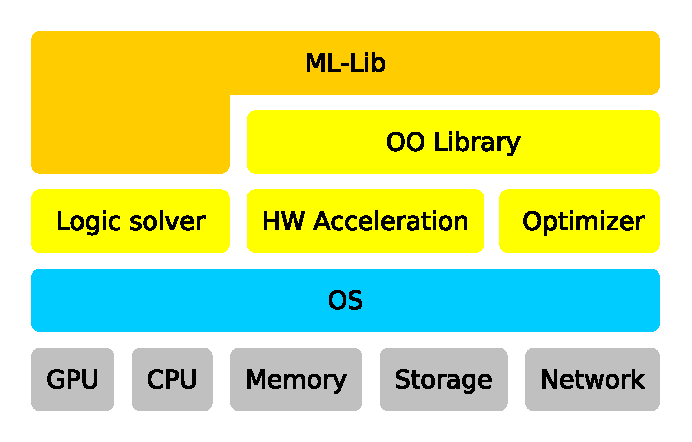
\includegraphics[width=.5\linewidth]{figures/mllib-layers.pdf}
    \caption[Layered view of our \mllib{}]{Layered view of our \mllib{}. An OO library is assumed behind the scenes, providing high-level abstraction to optimize ML predictors, possibly via HW acceleration}
    \label{fig:mllib-layers}
\end{figure}

The overall architecture is depicted in \cref{fig:mllib-layers}.
%
The \mllib{} assumes a goal-oriented logic solver being in place, where ordinary logic programs can be executed.
%
Thanks to the \mllib{}, these logic programs may also exploit a number of predicates aimed at training and using ML predictors---other than any other entity involved in the process.
%
Behind the scenes, the library also assumes an underlying object-oriented (OO) library providing high-level ML abstractions, such as datasets, predictors, and so on.
%
Examples of these libraries may be for instance Keras or \deeplearningforj{}.
%
The OO library may in turn be backed by an optimizer, i.e. a low-level software taking care of making training and data management effective on the available hardware---and possibly exploiting hardware acceleration (via GPU) to the purpose.
%
In practice, software such as Theano, Caffe, or Tensorflow may serve this purpose.
%
Actual technological choices may finally depend on the particular runtime platforms being targeted.
%
For instance, targeting the JVM may imply \deeplearningforj{} must be exploited behind the scenes, while targetting Python may pave the way towards the exploitation of both Keras and Tensorflow.
%
However, while technological choices are contingent and subject to change, the overall architecture is meant to support the implementation of the \mllib{} as a façade towards the underlying OO library, regardless of what it is.

\begin{sidewaysfigure}
    \centering
    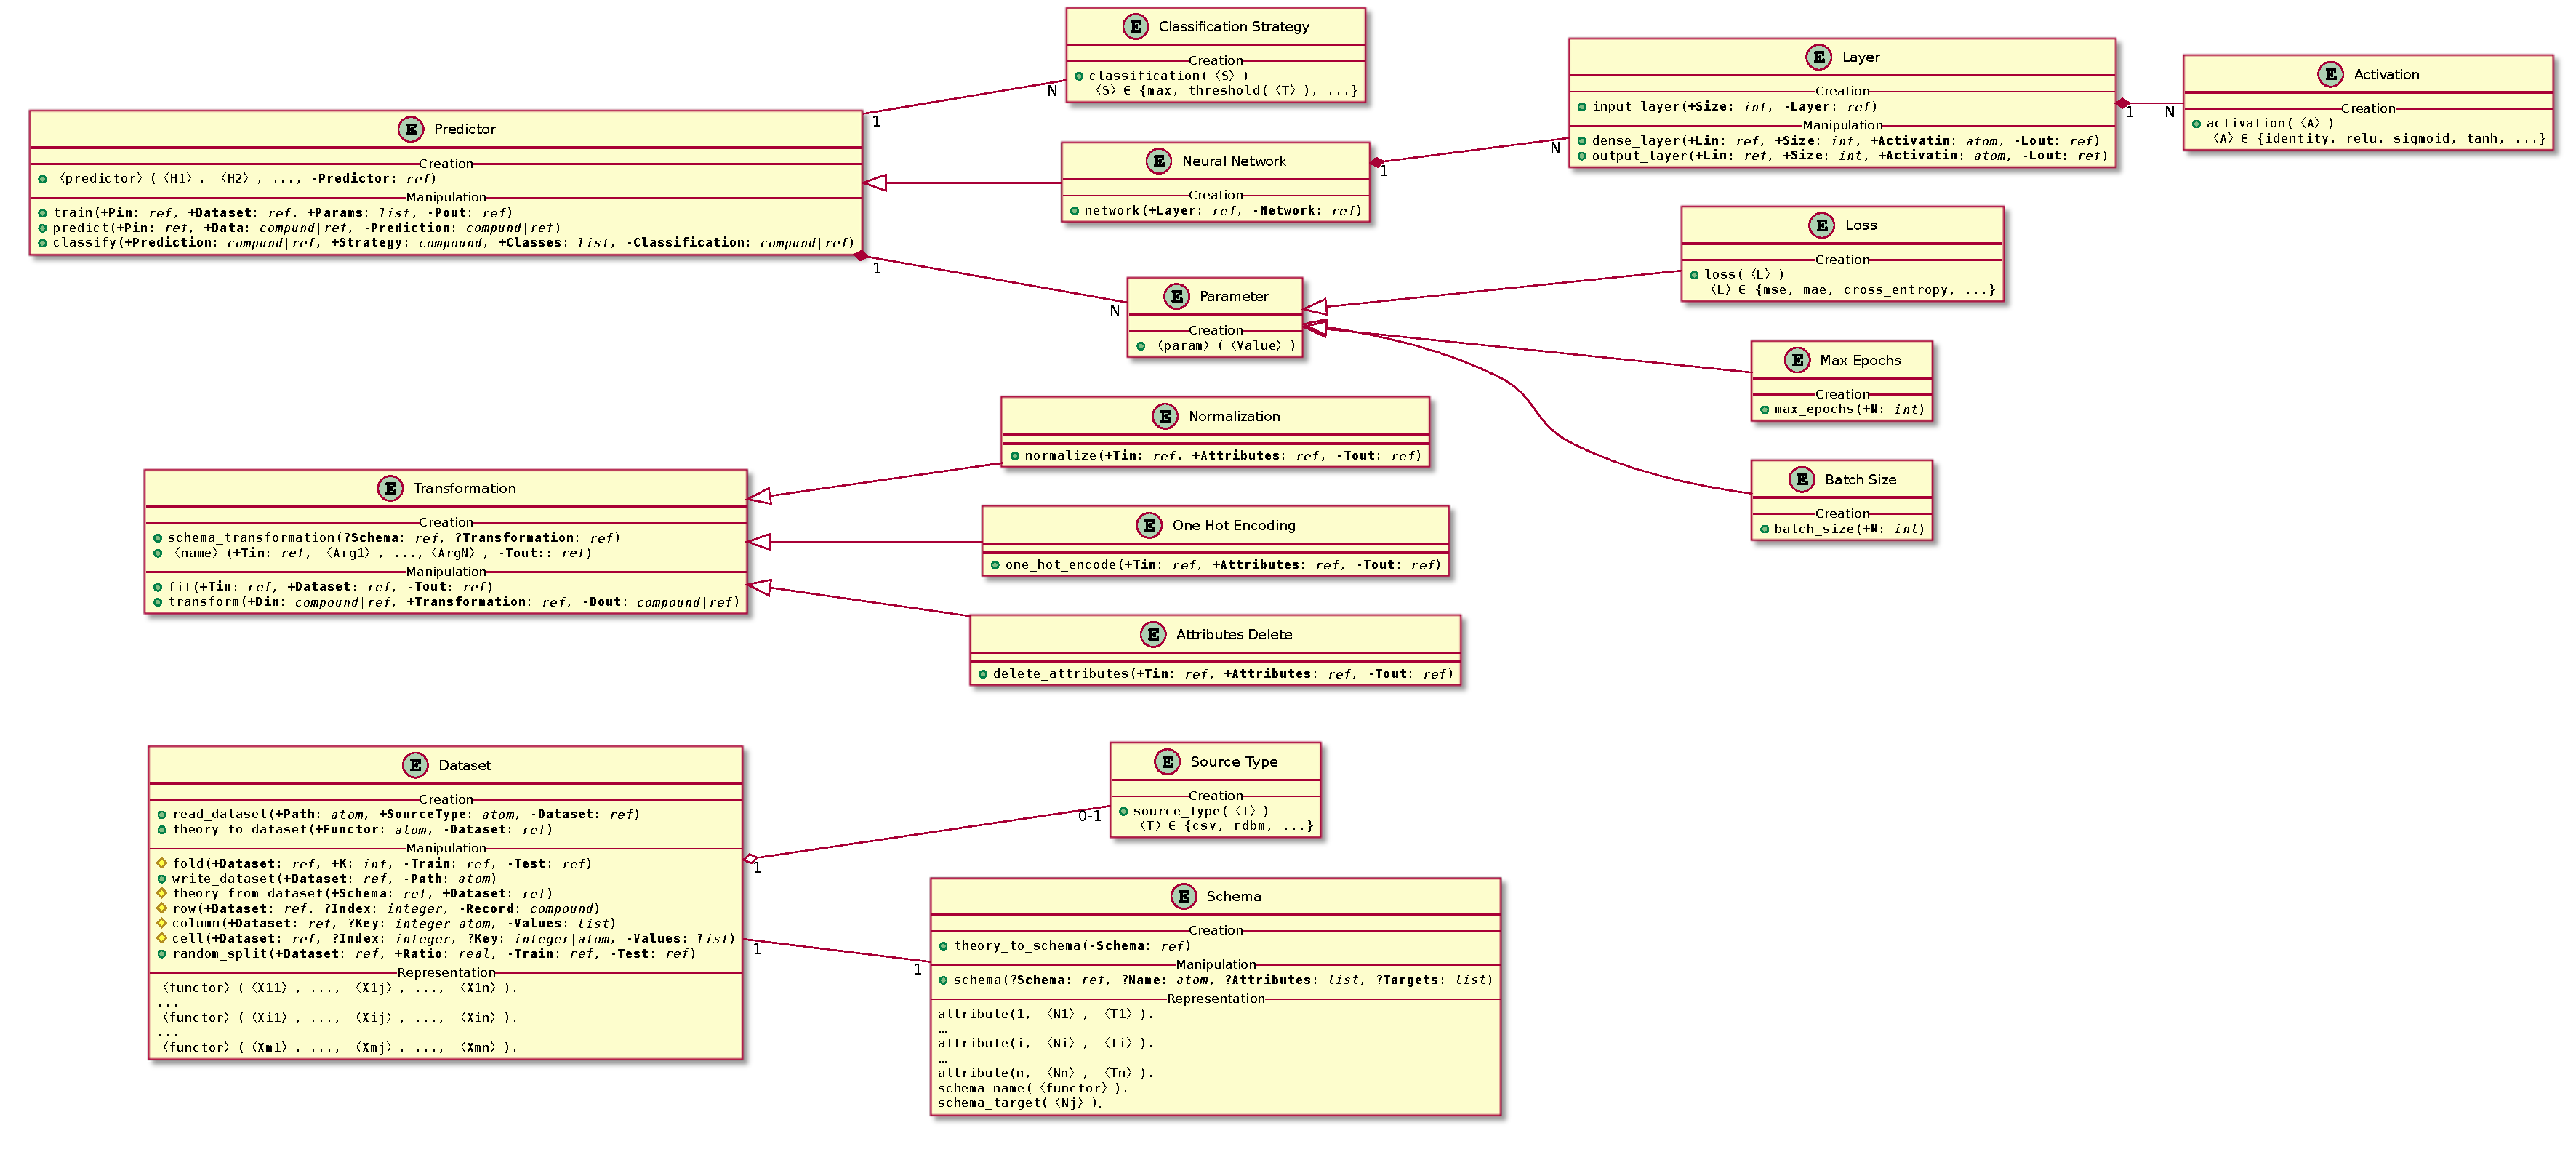
\includegraphics[width=\linewidth]{figures/entities.pdf}
    \caption[Overview of our \mllib{}'s design]{Overview of our \mllib{}'s design. The chart represents the many entities logic programmers may exploit via our \mllib{}, and the many predicates supporting their creation, manipulation, or representation. Predicates are depicted with either a yellow diamond in case they are non-deterministic (a.k.a. backtrackable), or a green circle otherwise.}
    \label{fig:design-overview}
\end{sidewaysfigure}

At the functional level, the design of our \mllib{} is provided in terms the entities from \cref{sec:requirements}, and the logic predicates available to create, manipulate, or represent them.
%
\Cref{fig:design-overview} provides an overview of these predicates, grouped by entities.
%
Both in the figure and in the reminder of this section, we adopt the following notation to denote the interfaces of logic predicates:
%
\begin{center}
    \pl{functor($\odot_1$ Name$_1$: \pli{type}$_1$, \ldots, $\odot_N$ Name$_N$: \pli{type}$_N$)}
\end{center}
%
where $N$ denotes the arity of predicate \pl{functor/$N$}, whose $i^{th}$ argument -- named \pl{Name$_i$} -- must be of type \pli{type$_i$}, and it must be considered as an input or output parameter depending on the mode indicator\footnotemark $\odot_i$.
%
\footnotetext{\url{cf. https://www.swi-prolog.org/pldoc/man?section=preddesc}}
%
So, for instance, we denote input parameters by \pl{+}, output parameters by \pl{-}, and input-output parameters by \pl{?}.
%
Admissible arguments types include constant term types (\pl{integer}, \pl{real}, \pl{atom}), structured term types (\pl{compound}, \pl{list}), as well as \emph{references} (\pl{ref}), and union types (\pl{T$_1$|T$_2$|$\ldots$}).
%
References, in particular, are a special kind of constant term, whose instances represent objects from the object-oriented realm.
%
These are necessary to make our \mllib{} able to operate with the non-logic entities exposed by the underlying OO library supporting ML.

Accordingly, in the reminder of this section, we enumerate the predicates constituting our \mllib{}, categorised w.r.t. the entities they act upon.
%
In particular, the \mllib{} exposes predicates covering 4 major sorts of entities -- i.e. the ones elicited in \cref{ssec:modelling}, namely: Schema, Dataset, Transformation, and Predictor --, plus a number of ancillary entities aimed at supporting their manipulation -- such as Classification Strategy, Source Type, and Parameter -- or specialising their behaviour---such as Neural Network, and Layer.

\subsection{Schemas}
\label{ssec:schemas}

Schemas are concise metadata describing datasets' columns.
%
They define their indexes, names, and admissible types, and they are assumed to be declared by the user.

The \mllib{} supports schemas represented as any of two forms: either as clauses or as objects---to be represented in LP via reference terms.
%
Ad-hoc predicates are provided to support the conversion from one form to the other.

\paragraph{Schemas as clauses}

In the general case, schema declarations are firstly provided by the user in clausal form.
%
This requires the user to fill the logic theory with clauses of the form:
%
\begin{center}
    \begin{tabular}{l}
        \pl{attribute($1$, $N_1$, $T_1$).}
        \\
        \qquad\vdots
        \\
        \pl{attribute($i$, $N_i$, $T_i$).}
        \\
        \qquad\vdots
        \\
        \pl{attribute($n$, $N_n$, $T_n$).}
        \\
        \pl{schema\_name($N$).}
        \\
        \pl{schema\_targets([$N_j$, $N_k$, $\ldots$, $N_h$]).}
    \end{tabular}
\end{center}
%
where $N$ is the name of the schema, and $n$ is the total amount of attributes declared for that schema, while $N_i$ is the name of the $i^{th}$ attribute, and $T_i$ is its type.
%
Indexes $j,k,h \in \{ 1, \ldots, n \}$ aim at selecting attributes names declared as \emph{targets}---i.e. as outputs of the learning process.
%
While attribute ($N_i$) and schema ($N$) names are simple atoms, attribute types ($T_i$) are compound terms for which the \pl{attribute\_type($T_i$)} holds true.

The \pl{attribute\_type/1} predicate is defined as follows:
%
\begin{center}
    \begin{tabular}{l}
        \pl{attribute\_type(\pli{string}).}
        \\
        \pl{attribute\_type(\pli{integer}).}
        \\
        \pl{attribute\_type(\pli{real}).}
        \\
        \pl{attribute\_type(\pli{boolean}).}
        \\
        \pl{attribute\_type(\pli{categorical}([\_ | \_])).}
        \\
        \pl{attribute\_type(\pli{ordinal}([\_ | \_])).}
    \end{tabular}
\end{center}
%
Hence, admissible attribute types involve infinite domains such as the numeric (either integer or real numbers), and strings ones, as well as finite domains such as booleans, and categorical (i.e. unordered) or ordinal sets of constant values.

\paragraph{Schemas as objects}

To be exploitable by the underlying OO library, schemas must be represented as objects.
%
Schemas represented in clausal form can be converted into object form via the following predicate:
%
\begin{center}
    \pl{theory\_to\_schema(-Schema: \pli{ref})}
\end{center}
%
which
%
\begin{inlinelist}
    \item inspects the current KB looking for a schema description in clausal form,
    \item instantiates a new schema object in the underlying OO library,
    \item creates a new reference term referencing the newly created schema,
    \item unifies that term with the output parameter denoted by \pl{Schema}.
\end{inlinelist}

References to schemas in object form may be then passed as arguments to many other predicates from the \mllib{} in order to provide them the necessary metadata to manipulate datasets.

\paragraph{Manipulating schemas}

A part from schema declaration or creation, other relevant operations over schemas involve the inspection (i.e. reading) of their components---namely, names, attribute names, attribute types, and targets.
%
This can be achieved via the following predicate:
%
\begin{center}
    \pl{schema(?Schema: \pli{ref}, ?Name: \pli{atom}, ?Attributes: \pli{list}, ?Targets: \pli{list})}
\end{center}
%
Given a schema reference, the predicate retrieves
%
\begin{inlinelist}
    \item the schema's name, which is unified with \pl{Name},
    \item the list schema attributes -- where each attribute has the form \pl{attribute($i$, $N_i$, $T_i$)} --, which is unified with \pl{Attributes}, and
    \item the list of schema targets -- where each target is an atom acting as attribute name --, which is unified with \pl{Targets}.
\end{inlinelist}
%
Notably, the predicate is \emph{bi-directional} and its arguments can act as either input or output parameters.
%
In case an unbound \pl{Schema} variable is provided as output parameter, and assuming that the \pl{Name}, \pl{Attributes}, and \pl{Targets} parameters are fully instantiated, the \pl{schema/4} predicate acts as yet another way to create a schema in object form---and the newly created schema is bound to \pl{Schema}.

\subsection{Datasets}

A dataset is a tabular representation of a bunch of homogenous data records.
%
As such, a dataset is characterised by a schema and a number of records matching that schema.

Similarly to what it does for schemas, the \mllib{} supports datasets represented as either clauses or objects.
%
Ad-hoc predicates are provided to support the conversion from one form to the other, other than for loading datasets from some data source, such as a file or a DBMS.

\paragraph{Datasets as objects}

In the general case, datasets objects are firstly loaded from a data source.
%
These may be local or remote files -- commonly in ``comma separated values'' (CSV) format --, as well as DBMS of any sort---provided that adequate connection support is provided by the underlying OO library, or any other third-party module.
%
The \mllib{} provides a unique entry point to load a dataset from any data source, namely:
%
\begin{center}
    \pl{read\_dataset(+Location: \pli{atom}, +SourceType: \pli{atom}, -Dataset: \pli{ref})}
\end{center}
%
This predicate aims at loading the dataset from a given \pl{Location}---be it a path on the local filesystem, a URL referencing some remote resource, or a connection string for some DBMS.
%
It also requires the caller to specify the \pl{SourceType} the dataset should be read from.
%
Regardless of the particular location and source type, the behaviour of the \pl{read\_dataset/3} predicate is such that:
%
\begin{inlinelist}
    \item raw data is retrieved from \pl{Location}, and
    \item parsed according to the selected source \pl{SourceType}; finally
    \item a new dataset object is created along with a reference term for it,
    \item which is then unified with \pl{Dataset}.
\end{inlinelist}

Admissible values for the \pl{SourceType} parameter are determined by the \pl{source\_type/1} predicate, defined as follows:
%
\begin{center}
    \begin{tabular}{l}
        \pl{source\_type(\pli{csv}).}
        %        \\
        %        \pl{source\_type(\pli{jdbc}).}
    \end{tabular}
\end{center}
%
meaning that currently the \mllib{} only supports data provisioning from CSV files.
%
However, further source types are going be supported in the future.
%
That will imply extending the \pl{source\_type/1} predicate definition with further cases.

\paragraph{Datasets as clauses}

Logic programmers may also be willing to describe the dataset via a logic theory.
%
When this is the case, the theory should contain not only the clauses describing the schema (i.e. the dataset's columns), but also a number of clauses describing the actual content of the dataset (i.e. its rows).
%
In particular, the \mllib{} expects data entries to be provided as clauses of the form:
%
\begin{center}
    \begin{tabular}{c}
        \pl{$N$(X$_{1,1}$, \ldots, X$_{1,j}$, \ldots, X$_{1,n}$).}
        \\
        \vdots
        \\
        \pl{$N$(X$_{i,1}$, \ldots, X$_{i,j}$, \ldots, X$_{i,n}$).}
        \\
        \vdots
        \\
        \pl{$N$(X$_{m,1}$, \ldots, X$_{m,j}$, \ldots, X$_{m,n}$).}
    \end{tabular}
\end{center}
%
where $N$ is the schema name declared via \pl{schema\_name/1}, and \pl{X$_{i,j}$} is the value of the $j^{th}$ attribute of the $i^{th}$ data entry.
%
Of course, the actual type of \pl{X$_{i,j}$} must be coherent with the formal type $T_i$ declared in the schema definition.

Datasets in clausal form must be converted into object form to be exploitable by the underlying OO library.
%
This can be achieved via the following predicate:
%
\begin{center}
    \pl{theory\_to\_dataset(+SchemaName: \pli{atom}, -Dataset: \pli{ref})}
\end{center}
%
which
%
\begin{inlinelist}
    \item inspects the current KB looking for one or clauses using \pl{SchemaName} as the head functor,
    \item instantiates a new dataset object in the underlying OO library,
    \item populates it with as many rows as the aforementioned clauses,
    \item creates a new reference term referencing the newly created dataset,
    \item unifies that term with the output parameter denoted by \pl{Dataset}.
\end{inlinelist}
%
Of course, this predicate also takes into account the schema-related metadata which are assumed to be defined in clausal form as well.

\paragraph{Datasets manipulation}

Datasets are amongst the basic bricks of predictors training in ML, hence they must support several kinds of manipulations.
%
Within the scope of the \mllib{}, we support partitioning a dataset in several ways to support both cross validation and test set separation, other than accessing a dataset by row, column, or cell.
%
Conversions from and into clausal form complete the picture.

\subparagraph{Splitting}

To support test set separation, the \mllib{} provides a predicate to randomly split a dataset into a training and test set, given a ratio:
%
\begin{center}
    \pl{random\_split(+Dataset: \pli{ref}, +Ratio: \pli{real}, -Train: \pli{ref}, -Test: \pli{ref})}
\end{center}
%
Given a reference to a \pl{Dataset} in object form, and a \pl{Ratio} -- i.e. a real number in the range $]0,1[$ --, the predicate
%
\begin{inlinelist}
    \item randomly samples the given percentage of data entries from \pl{Dataset},
    \item collects them into a new dataset, whose reference is bound to \pl{Test}, and
    \item collects the remaining data entries into yet another dataset, whose reference is bound to \pl{Train}.
\end{inlinelist}
%
So, for instance, a ratio of $0.1$ would randomly split the dataset into a training set containing 90\% of the original data, and a test set containing 10\% of the original data.

To support cross validation, \mllib{} provides an \textit{ad-hoc} predicate:
%
\begin{center}
    \pl{fold(+Dataset: \pli{ref}, +K: \pli{integer}, -Train: \pli{ref}, -Validation: \pli{ref})}
\end{center}
%
which splits the \pl{Dataset} into 2 partitions, namely \pl{Train} and \pl{Validation}, the former containing $\frac{k-1}{k}$\% data entries -- to be used as the training set --, and the latter containing the remaining $\frac{1}{k}$\% data entries---to be used as the validation set.
%
Both \pl{Train} and \pl{Validation} are bound to reference terms, referencing datasets in object form.
%
Notably, the \pl{fold/2} is non-deterministic as it enumerates all possible folds of a \pl{K}-fold cross validation process.
%
Hence, provided that $\pl{K} \geq 2$, the predicate computes \pl{K} partitioning of the original dataset.

\subparagraph{Data access}

The \mllib{} supports accessing the information encapsulated into a dataset in object form via three predicates, namely:
%
\begin{center}
    \pl{row(+Dataset: \pli{ref}, ?Index: \pli{integer}, -Values: \pli{list}).}
    \\
    \pl{column(+Dataset: \pli{ref}, ?Attribute: \pli{integer}|\pli{atom}, -Values: \pli{list}).}
    \\
    \pl{cell(+Dataset: \pli{ref}, ?Index: \pli{integer},  ?Attribute: \pli{integer}|\pli{atom}, -Values: \pli{list}).}
\end{center}
%
They all are non-deterministic, and they both support the retrieval of a particular row / column / cell from the dataset as well as the enumeration of all possible rows / columns / cells from that dataset.

In particular, predicate \pl{row/3} aims at retrieving rows.
%
If the \pl{Index} parameter is a positive integer, then the predicate attempts to unify the \pl{Value} parameter with the list of values contained the \pl{Index}$^{th}$ row of the dataset.
%
Otherwise, if \pl{Index} is uninstantiated, the predicate enumerates all rows in the dataset, and for each row it unifies the \pl{Index} and \pl{Values} parameters accordingly.

The predicate \pl{column/3} is totally analogous to \pl{row/3}, expect it aims at retrieving or enumerating columns.
%
The only notable difference w.r.t. \pl{row/3} is that columns can be referenced by either attribute names or indexes---thus both positive integers and atoms can be bound to the \pl{Attribute} parameter.

Finally, predicate \pl{cell/4} supports accessing or enumerating cells.
%
In particular, it allows the user to access the \pl{Value} in position $(\pl{Index}, \pl{Attribute})$, where \pl{Index} is a row index in and \pl{Attribute} is an attribute name or index.
%
If one or both parameters are uninstantiated, the predicate enumerates all possible assignments.

\subparagraph{Object to clausal form conversion}

The logic programmer may also be willing to convert a dataset in object form into a dataset in clausal form.
%
This can be attained via the following predicate:
%
\begin{center}
    \pl{theory\_from\_dataset(+Schema: \pli{ref}, +Dataset: \pli{ref})}
\end{center}
%
Given the references to both a dataset and its schema in object form, the predicate populates the solver's \emph{dynamic} KB with the a number of clauses representing the dataset and its schema in the clausal form described above.

\subsection{Transformations}

A transformation is a function altering a dataset and, possibly, its schema.
%
It may be parametric and hence tuned according to the content of the dataset or its schema.

Consider for instance the case of the ``Normalization'' transformation.
%
It applies an affine transformation to each column of the dataset (independently) in such a way that it has a predefined mean (e.g. 0) and standard deviation (e.g. 1).
%
Hence, it alters the content of a dataset leaving its schema unaffected.
%
To work properly, it requires two major computational steps, namely
%
\begin{inlinelist}
    \item computing (and storing) the mean and standard deviation of each column of the original dataset,
    \item applying the affine transformation to normalize the dataset columns (i.e. subtracting the mean and dividing by the standard deviation each cell of each column).
\end{inlinelist}

In the general case, transformations are modelled as \emph{stateful} entities supporting at least 2 operations, namely \emph{fitting} and \emph{transforming} a dataset and its schema.
%
The latter operation is also known as ``applying a transformation to a dataset'', and it should not only support the retrieval of the transformed dataset, but the transformed schema as well.
%
Furthermore, transformations should be composable into \emph{pipelines}, i.e. cascades of simpler transformations to be fitted or applied in a row.

To support all such aspects, the \mllib{} provides predicates aiming to
%
\begin{enumerate}
    \item\label{tr:create} create a transformation given a schema,
    \item\label{tr:combine} combine elementary transformations into composite transformations,
    \item\label{tr:fit} fit transformations over data (regardless of whether they are elementary or composite),
    \item\label{tr:transform} apply composite or elementary transformation to a dataset, thus attaining a new dataset,
    \item\label{tr:get-schema} retrieve the new schema resulting from a transformation application.
\end{enumerate}
%
Differently from schemas and datasets, for which the \mllib{} supports both clausal and object representations, transformations are only representable in object form, hence the following predicates assume transformations to be manipulated via reference terms.

\paragraph{Transformations to/from schemas}

To support aims \ref{tr:create} and \ref{tr:get-schema}, the \mllib{} provides the following \emph{bi-directional} predicate:
%
\begin{center}
    \pl{schema\_transformation(?Schema: \pli{ref}, ?Transformation: \pli{ref})}
\end{center}
%
which changes its behaviour depending on which arguments are instantiated.

In particular, if \pl{Schema} is bound to a schema object, then \pl{Transformation} is unified with an identity transformation -- i.e. a transformation leaving the schema and the dataset unaffected --, which can be used as the initial step of a composite pipeline.
%
This is how aim \ref{tr:create} is served.

Conversely, if \pl{Transformation} is bound to an actual transformation object, then \pl{Schema} is unified with the new schema object attained by applying that transformation to the schema it was originally constructed from.
%
This is how aim \ref{tr:get-schema} is served.

\paragraph{Creating and combining elementary transformations}

To support aim \ref{tr:combine},  the \mllib{} provides a number of predicates sharing a similar syntax.
%
Each predicate is in charge of creating a composite transformation by appending a specific elementary transformation to some previously created one---like, for instance, the identity transformation created via \pl{schema\_transformation/2}.
%
%While we just describe the general syntax here, the actual predicates are described later in this section.

In the general case, the combination and creation of transformations is attained via predicates of the form:
%
\begin{center}
    \pl{$\langle \mathit{name} \rangle$(+Pipeline$_{in}$: \pli{ref}, +$A_1$, \ldots, +$A_n$, -Pipeline$_{out}$: \pli{ref})}
\end{center}
%
where $\langle \mathit{name} \rangle$ is the name of the transformation being appended to \pl{Pipeline$_{in}$}, while $A_1, \ldots, A_n$ are transformation-specific parameters, and \pl{Pipeline$_{out}$} is the output parameter to which the newly created transformation is bound.

The \mllib{} currently supports 3 predicates of this sort, and further ones may be defined following the same syntactical convention.
%
These are \pl{normalize/3}, \pl{one\_hot\_encoding/3}, and \pl{attributes\_delete/3}, and their details are described later in this paragraph.
%
Here we focus on the overall design which is aimed at supporting the declaration of \emph{pipelines} of transformations, via conjunctions of goals:
%
\begin{center}
    \begin{tabular}{l}
        \pl{theory\_to\_schema(OriginalSchema),}
        \\
        \pl{schema\_transformation(OriginalSchema, T$_0$),}
        \\
        \pl{transformation$_1$(T$_0$, arg$_1$, T$_1$),}
        \\
        \qquad\vdots
        \\
        \pl{transformation$_m$(T$_{m-1}$, arg$_m$, T$_m$),}
        \\
        \pl{schema\_transformation(FinalSchema, T$_m$)}
    \end{tabular}
\end{center}
%
Following this convention, logic programmers may declaratively construct the pipeline of transformations to be applied to \pl{OriginalSchema} to produce \pl{FinalSchema}, in such a way that each variable \pl{T$_i$}, for $i \in \{0, \ldots, m\}$ is bound to an object summarising all transformation steps from $0$ to $i$.

\subparagraph{Normalization}

A dataset's columns can be normalised in such a way that, for each column, the mean is 0 and the standard deviation is 1.
%
Such kind of transformations may alter the dataset while leaving its schema unaffected.
%
A normalization transformation can be created via the following predicate:
%
\begin{center}
    \pl{normalize(+Pipeline$_{in}$: \pli{ref}, +Attributes: \pli{list}|\pli{atom},
        \\
        -Pipeline$_{out}$: \pli{ref})}
\end{center}
%
There, parameter \pl{Attributes} must be bound to either a list of attribute names or indexes -- denoting the columns to be normalized --, or the `\pl{all}' atom---denoting a situation where all columns should be normalized.

\subparagraph{One Hot Encoding}

A dataset's target attributes whose type are categorical with $k$-admissible values can be replaced by $k$ binary attributes, via one-hot encoding (OHE) transformations.
%
Such kind of transformations alter both the dataset and its schema.
%
A OHE transformation can be created via the following predicate:
%
\begin{center}
    \pl{one\_hot\_encode(+Pipeline$_{in}$: \pli{ref}, +Attributes: \pli{list}|\pli{atom}, -Pipeline$_{out}$: \pli{ref})}
\end{center}
%
There, parameter \pl{Attributes} must be bound to a list of attribute names or indexes denoting the columns to be one-hot encoded.

\subparagraph{Attributes Deletion}

Columns may be dropped from a dataset and its schema via attribute deletion transformations.
%
Such kind of transformations alter both the dataset and its schema.
%
An attribute deletion transformation can be created via the following predicate:
%
\begin{center}
    \pl{one\_hot\_encode(+Pipeline$_{in}$: \pli{ref}, +Attributes: \pli{list}|\pli{atom}, -Pipeline$_{out}$: \pli{ref})}
\end{center}
%
There, parameter \pl{Attributes} must be bound to a list of attribute names or indexes denoting the columns to be dropped.

\paragraph{Fitting transformations to data}

To support aim \ref{tr:fit}, the \mllib{} provides the following predicate:
%
\begin{center}
    \pl{fit(+Transformation$_{in}$: \pli{ref}, +Dataset: \pli{ref},
        \\
        -Transformation$_{out}$: \pli{ref})}
\end{center}
%
which works by tuning \pl{Transformation$_{in}$} over \pl{Dataset}, producing a new transformation, whose reference is unified with \pl{Transformation$_{out}$}.

The new transformation may be identical to the input one, in case the latter does not require tuning---such as in the case of OHE.
%
Conversely, in case it does need tuning -- as in the case of normalization --, the output transformation may actually be different than the original one.
%
Fitting a composite transformation of course has the effect of fitting all its components, recursively.

\paragraph{Applying transformations to data}

Finally, to support aim \ref{tr:transform}, the \mllib{} provides the following \emph{bi-directional} predicate:
%
\begin{center}
    \pl{transform(?Data$_{in}$: \pli{ref}|\pli{compound}, +Transformation: \pli{ref},
        \\
        ?Data$_{out}$: \pli{ref}|\pli{compound})}
\end{center}
%
which can either apply a transformation or its inverse depending on either entire datasets or their rows, depending on how arguments are passed.

In particular, \pl{Data$_{in}$} and \pl{Data$_{out}$} can be either dataset references, or compound terms, denoting single rows.
%
Of course, applying a (possibly inverse) transformation to a row (resp. entire dataset) shall produce a row (resp. entire dataset) in return.

The predicate applies \pl{Transformation} to \pl{Data$_{in}$} in case the latter parameter is instantiated, unifying the transformed result with \pl{Data$_{out}$}.
%
Conversely, it applies the inverse of \pl{Transformation} to \pl{Data$_{out}$} in case the \pl{Data$_{in}$} parameter is uninstantiated while the former is not.
%
When this is the case, the transformed result is unified with \pl{Data$_{in}$}.

\subsection{Predictors}

Predictors are stateful entities which can be \emph{trained} over a dataset to later draw \emph{predictions} on new data matching the same schema.
%
In the general case, all predictors may require a number of \emph{hyper parameters} to be specified upon creation, and a number or \emph{learning parameters} to be provided upon training.
%
Both kinds of parameters aim at regulating the predictor behaviour, either in general or during training, and their actual values must be decided by the user.

Given the large number of possible predictors from the data science literature, the \mllib{} just fixes the syntactical convention to support predictors creation, other than the API to support both training and drawing predictions.
%
Notably, as for transformations, the \mllib{} assumes predictors to be represented in object form, and therefore manipulated via reference terms.

\paragraph{Creating predictors}

The \mllib{} constrains predictor-creating predicates to comply to the following syntactical convention:
%
\begin{center}
    \pl{$\langle \mathit{name} \rangle$(+$H_1$, \ldots, +$H_n$, -Predictor: \pli{ref})}
\end{center}
%
where $\langle \mathit{name} \rangle$ is the name of the predictor type being instantiated, while $H_1, \ldots, H_n$ are predictor-type-specific hyper-parameters, and \pl{Predictor} is the output parameter to which the newly created predictor is bound.

The \mllib{} currently supports one predicate of this sort -- namely, the \pl{neural\_network/2} predicate, described later in this section --, yet further ones may be defined following the same syntactical convention.

\paragraph{Training}

Regardless of their nature, predictors can be trained on data via the following predicate:
%
\begin{center}
    \pl{train(+Predictor$_{in}$: \pli{ref}, +Dataset: \pli{ref}, +Params: \pli{list}, -Predictor$_{out}$: \pli{ref})}
\end{center}
%
The predicate accepts \pl{Predictor$_{in}$} as the predictor to be trained, the \pl{Dataset} it should be trained upon, and a list of predictor-specific \pl{Params}.
%
Behind the scenes, the predicate exploits a predictor-specific learning algorithm to train \pl{Predictor$_{in}$}, possibly following the suggestions/constraints carried by \pl{Params}.
%
Once the training has been completed, a reference to the trained predictor is bound to \pl{Predictor$_{out}$}, and the execution of the predicate succeeds.

\subparagraph{Learning Parameters}

The \pl{Params} argument of \pl{train/4} must be instantiated with a list of learning parameters aimed at controlling and constraining the execution of a learning algorithm.
%
In the general case, each parameter is a term of the form:
%
\begin{center}
    \pl{$\langle \mathit{name} \rangle$($\langle \mathit{value} \rangle$)}
\end{center}
%
where $\langle \mathit{name} \rangle$ is a functor describing the purpose of the parameter, while $\langle \mathit{value} \rangle$ is an arbitrary term acting as value for the parameter.

In the particular case of neural networks, the \mllib{} admits the following learning parameters
%
\begin{itemize}
    \item \pl{max\_epochs(N: \pli{integer})} limiting the amount of epochs\footnotemark{} to be performed while training a NN;
    \footnotetext{i.e., the amount of times the learning algorithm works through the entire training dataset}

    \item \pl{batch\_size(N: \pli{integer})} defining the amount of training samples to be taken into account in each single step of the learning algorithm;

    \item \pl{learning\_rate(R: \pli{real})} defining the step size in a gradient descent learning process;

    \item \pl{loss(Function: \pli{atom})} dictating which loss function should be optimised during training (admissible values include: \pl{mse} for mean squared error, \pl{mae} for mean absolute error, \pl{cross\_entropy}, etc.)
\end{itemize}
%
Other sorts of learning parameters may be added to the \mllib{}, targeting both NN or other sorts of predictors.

\paragraph{Drawing predictions}

Regardless of their nature, \emph{trained} predictors can be exploited to draw predictions from data -- e.g. from a whole dataset or a single row --, via the following predicate:
%
\begin{center}
    \pl{predict(+Predictor: \pli{ref}, +InputData: \pli{ref}|\pli{compound}, -Prediction: \pli{ref}|\pli{compound})}
\end{center}
%
The predicate accepts a \pl{Predictor} (which must have been previously trained via \pl{train/4}), and some \pl{InputData} -- which may either be reference to a dataset object, or a compound term denoting a single row --, and uses the \pl{Predictor} to compute a prediction for each data entry in \pl{InputData}.
%
Predictions may consist of either a single row or a whole dataset, depending on how many data entries are contained in \pl{InputData}.
%
In both cases, the \pl{Prediction} output parameter is unified with the predicted row/dataset.

In case \pl{InputData} is bound to a full dataset including one or more target columns, those target columns are ignored while computing predictions.
%
Conversely, when \pl{InputData} is bound to a list of values, the \mllib{} considers them all as input values.

\subparagraph{Classification}

As many predictors -- there including NN -- are technically tailored on \emph{regression} tasks (where predicted values are real numbers), it is a common practice for data scientists to map \emph{classification} tasks (where predicted values are categorical) onto regression tasks, to make it possible to address them via regressors.
%
The mapping commonly works as follows.
%
A classification task requiring input data to be classified according to $k \in \mathbb{N}_{\geq 0}$ classes, can be conceived as a regression aimed at predicting continuos vectors $\mathbf{y} \in \mathbb{R}^k$ from the same input data.
%
Given a particular input datum $\mathbf{x}$, and the corresponding prediction $\mathbf{y}$, the $i^{th}$ component of $\mathbf{y}$ -- namely, $y_i$ -- could then be interpreted as the confidence of $\mathbf{x}$ being classified as an example of the $i^{th}$ class.
%
Depending on the nature of the classification task at hand, the confidence values in $\mathbf{y}$ could be jointly interpreted following several strategies.
%
In a situation where classes are mutually exclusive, one may use function ${argmax}_i(y_i)$ to select the most likely class of $\mathbf{x}$.
%
Otherwise, if classes can overlap, one choose a confidence threshold $\theta$ and classify $\mathbf{x}$ according to all those classes $i$ such that $y_i \geq \theta$.

The \mllib{} supports classification out of regressors via the following predicate:
%
\begin{center}
    \pl{classify(+Prediction: \pli{ref}|\pli{compound}, +Strategy: \pli{compound}, +Classes: \pli{list}, -Classification: \pli{ref}|\pli{compound})}
\end{center}
%
which accepts a \pl{Prediction} computed via \pl{predict/3} -- be it a single row or a whole dataset --, a classification \pl{Strategy}, a list of \pl{Classes}, and an output parameter, \pl{Classification}, which is bound to a container for as many categorical predictions as in \pl{Prediction}.

Notably, while the \pl{Classes} parameter must consist of a list of (at least 2) class names, admissible values for the \pl{Strategy} parameter are determined by the \pl{classification/1} predicate, defined as follows:
%
\begin{center}
    \begin{tabular}{l}
        \pl{classification(\pli{argmax}).}
        \\
        \pl{classification(\pli{threshold}(Th)) :- numeric(Th).}
    \end{tabular}
\end{center}
%
meaning that currently the \mllib{} only supports classification via the $\mathtt{argmax}$ or threshold-based strategies---despite further strategies may be added following the same syntactical notation.

\subparagraph{Assessing Predictions}

Predictors can be assessed by comparing their \emph{actual} predictions with a test dataset containing \emph{expected} predictions, having no overlap with the data used during training.
%
Several scoring functions can be used to serve this purpose, like, for instance mean squared/absolute error (MSE/MAE) or R$^2$ for regressors, as well as accuracy, recall, or F1-Score for classifiers.

The \mllib{} supports assessing a predictor via a number of predicates following the same syntactical convention:
%
\begin{center}
    \pl{$\langle \mathit{name} \rangle$(+Actual: \pli{ref}|\pli{list}, +Expected: \pli{ref}|\pli{list}, -Score: \pli{real})}
\end{center}
%
where $\langle \mathit{name} \rangle$ is the name of the scoring function of choice, \pl{Actual} is either a dataset or a list containing the actual predictions produced by the predictor under assessment, \pl{Actual} is either a dataset or a list containing the test data, and \pl{Score} is the output parameter to be unified with the score value computed whenever the predicate is executed.

Notable cases of scoring functions are, for instance: \pl{mse/3}, \pl{mae/3}, \pl{r2/3}, \pl{accuracy/3}, \pl{recall/3}, or \pl{f1\_score/3}, while further ones may be added following the same syntactical convention.

\subsubsection{Neural Networks}

Neural networks are a particular sort of predictor.
%
They consist of directed acyclic graphs (a.k.a. DAG) where vertices are elementary computational units called neurons, and edges (a.k.a. synapses) are weighted.

Topologically, neural networks are organised in layers, and data scientists design them by specifying
%
\begin{inlinelist}
    \item how many layers compose the network,
    \item how many neurons compose each layer,
    \item which activation function is used by each layer -- and therefore by each neuron therein contained --, and
    \item how are layers -- and therefore their neurons -- interconnected with their predecessors and successors in the DAG.
\end{inlinelist}
%
Hence, a NN's hyper-parameters should provide information about such aspects.

The \mllib{} provides the following predicate to construct NN-like predictors:
%
\begin{center}
    \pl{neural\_network(+Topology: \pli{ref}, -Predictor: \pli{ref})}
\end{center}
%
There, \pl{Topology} is a reference to an object describing the overall architecture of the network, and, in particular its layers.

\paragraph{Layers}

Layered architectures are commonly composed by at least one input layer -- whose neurons simply mirror the input data --, and one output layer---whose neurons' output values jointly represent the NN prediction.
%
In the between an arbitrary amount of layers of different sorts may be defined---e.g. dense, convolutional, pooling, etc.
%
In all such cases, declaring a layer implies specifying its sort, size (in terms of neurons), and activation function.

The \mllib{} supports the declaration of layered architectures similarly to how it supports pipelines of transformations.
%
There are two major sorts of predicates to serve this purpose:
%
\begin{center}
    \pl{input\_layer(+Size: \pli{integer}, -Layer: \pli{ref}).}
    \\
    \pl{$\langle type \rangle$\_layer(+Previous: \pli{ref}, +Size: \pli{integer}, +Activation: \pl{ref}, -Layer: \pli{ref}).}
\end{center}

The former predicate, \pl{input\_layer/2}, aims at creating a \pl{Layer} of a given \pl{Size}.
%
The size should match the amount of input attributes in the training dataset.
%
This is the entry point of any cascade of predicates aimed at creating a layered architecture.

Conversely, the latter predicate pattern, \pl{$\langle type \rangle$\_layer/4} is matched by a number of actual predicates aimed at creating intermediate or output layers.
%
There $\langle type \rangle$ denotes the type of the layer.
%
Regardless of their type, these predicates accept a reference to some \pl{Previous} layer, whose output synapses are connected to the layer under construction, in a way which depends by its type.
%
They also accept the \pl{Size} of the layer to be constructed, and the \pl{Activation} function its neurons should employ.
%
Finally, they all accept an output parameter, \pl{Layer}, to which a reference to the newly created layer is bound, in case creation succeeds.

The \pl{dense\_layer/4} predicate is a notable case matching the aforementioned pattern.
%
It aims at declaring a layer whose neurons are \emph{densely} connected with its predecessor's ones---in the sense that, each neuron of the predecessor has an outgoing synapsis towards each neuron of the dense layer.
%
Layers of such a sort are commonly exploited as intermediate.
%
Conversely, layers declared via the \pl{output\_layer/4} predicate -- again matching the aforementioned pattern -- are commonly \emph{final} in any well formed NN architecture.

So, for instance, an ordinary multi-layered perceptron (MLP) composed by 1 input layer with 4 neurons, 1 hidden layer with 7 neurons, and 1 output layer with 3 neurons, where all neurons exploit the sigmoid activation function, can be declared as follows:
%
\begin{center}
    \begin{tabular}{l}
        \pl{input\_layer(4, I),}
        \\
        \pl{dense\_layer(I, 7, sigmoid, H),}
        \\
        \pl{output\_layer(H, 3, sigmoid, O),}
        \\
        \pl{neural\_network(O, NN)}
    \end{tabular}
\end{center}
%
There variable \pl{I} is bound to the input layer, variable \pl{H} is bound to the hidden layer, and \pl{O} is bound to the output layer, whereas \pl{NN} is bound to a MLP predictor whose architecture comprehends \pl{I}, \pl{H}, and \pl{O}.

\subparagraph{Activation Functions}

The behaviour of neurons should be finely tuned via their activation function.
%
Indeed, all layer-creating predicates of the form \pl{$\langle type \rangle$\_layer/4} expect an activation function to be provided by the user.
%
Admissible activation functions are regulated by the \pl{activation/1} predicate, defined below:
%
\begin{center}
    \begin{tabular}{lcl}
        \pl{activation(\pli{identity}).} & \qquad & denoting $f(x) = x$
        \\
        \pl{activation(\pli{sigmoid}).} & \qquad & denoting $f(x) = 1/(1+e^{-x})$
        \\
        \pl{activation(\pli{tanh}).} & \qquad & denoting $f(x) = \mathit{tanh}(x)$
        \\
        \pl{activation(\pli{relu}).} & \qquad & denoting $f(x) = \mathit{max}(0, x)$
    \end{tabular}
\end{center}
%
while others may be possibly added.

\section{Technology-related aspects}
\label{sec:tech}

The \mllib{} requires blending several programming paradigms and languages.
%
Indeed, it is intended to be used by logic programmers and via logic programs -- e.g. Prolog programs --, yet it explicitly requires some underlying OO library supporting ML facilities.
%
Hence, from a technical perspective, it requires at least
%
\begin{inlinelist}
    \item a LP technology supporting the definition of custom predicates, possibly triggering the execution of OO code
    \item an OO technology supporting the declaration, training, and exploitation of ML predictors.
\end{inlinelist}

In this section we discuss the choice of \twopkt{} as the underlying LP technology.
%
However, at the time of writing, this introduces a technological constraint on the JVM platform.
%
Hence, here we also report the technological selection process aimed at selecting the best OO technology supporting ML on the JVM.
%
Spoiler alert: we select \deeplearningforj{} (\dlfj{}) because of its superior maturity/usability trade-off.


\subsection{\twopkt{} as the underlying logic ecosystem}

\twopkt{}~\cite{cco-softwarex-2021-2pkt} is a logic ecosystem rebooting the tuProlog~\cite{tuprolog-padl01} project and providing a number of loosely coupled logic facilities, including but not limited to knowledge representation via terms and clauses, unification, and logic resolution.
%
In particular, \twopkt{} provides such facilities via a Kotlin-based object-oriented API, which eases the construction of applications where LP and OOP are blended together.
%
As a Kotlin library, \twopkt{} can currently run on the JS, JVM e Android platforms.

\begin{figure}
    \centering
    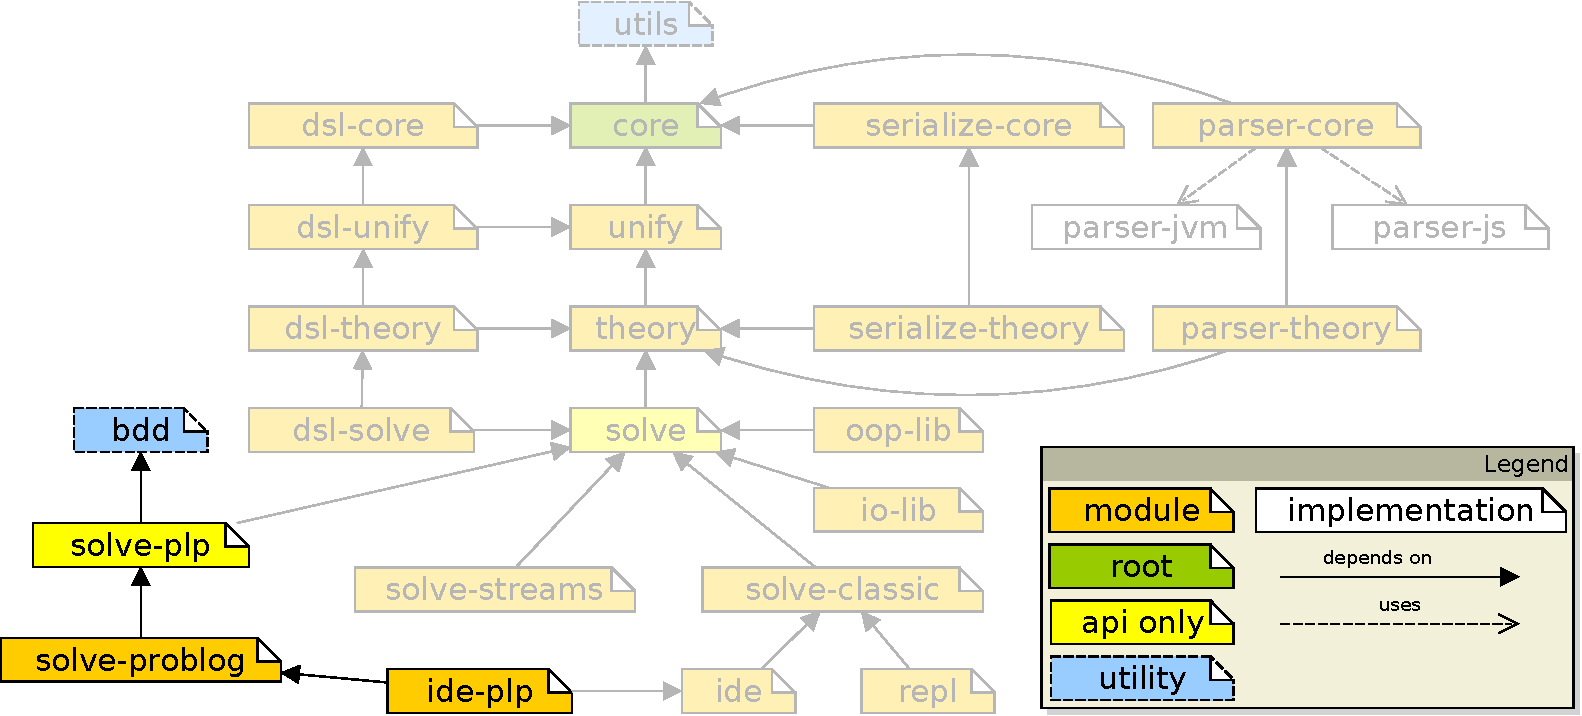
\includegraphics[width=0.8\linewidth]{figures/project-map.pdf}
    \caption{Localization of the \mllib{} into the \twopkt{} ecosystem}
    \label{fig:structure}
\end{figure}

As shown in \cref{fig:structure}, the \mllib{} is realised as yet another module extending the \twopkt{} ecosystem.
%
In particular, it builds upon
%
\begin{inlinelist}
    \item the knowledge representation facilities offered by the \module{core} module,
    \item the logic unification facilities offered by the \module{unify} module,
    \item the clause in-memory indexing facilities offered by the \module{theory} module,
    \item the general-purpose API for logic resolution offered by the \module{solve} module,
    \item the IO predicates offered by the \module{io-lib} module,
    \item the OOP$\leftrightarrow$LP interoperability facilities offered by the \module{oop-lib} module, other than, of course
    \item \dlfj{}.
\end{inlinelist}

With respect to LP solutions, \twopkt{} provides two particular facilities which are key enabler for the \mllib{}.
%
The first one is the notion of \emph{generator}, introduced in \cite{2pkt-jelia2021} and briefly summarised in \cref{sssec:generators}, while the second one is the notion of \emph{reference} term, described in \cref{sssec:ref-terms}.

\subsubsection{Generators for LP--OOP interoperability}\label{sssec:generators}

Briefly speaking, generators are gateways mediating the invocation of OO code from logic programs.
%
Thanks to generators, ordinary logic predicates can be implemented in OOP, in such a way that, whenever a goal $p(X_1, \ldots, X_n)$ is met as part of some resolution process, some corresponding OO function (i.e. the generator) is called.
%
The function may then exploit any OO facility available in the local runtime---there including any ML-related library.
%
Eventually, the function must \emph{lazily} return a (possibly infinite) stream of data, as well as a single result.
%
Each returned datum is interpreted back in logic as a solution for the goal $p/n$ which triggered the generator in the first place.
%
Each solution may then carry possible assignments for the variables $X_1, \ldots, X_n$, which may then be taken into account in the remainder of the resolution process.

So, essentially, generators allow for bi-directional communication among a logic solver and the underlying OO runtime.
%
Information may be propagates from the logic realm to the OO one as ordinary predicate arguments, instantiated at invocation time.
%
Information may be back-propagated from the OO realm to the logic one as variable assignments, instantiated at return time.

Generators are supported in \twopkt{} via the \module{solve} module.
%
Notably, they are the basic mechanism supporting the manipulation of schemas, datasets, transformations, and predictors in the \mllib{}.

\subsubsection{Reference Terms and the \module{oop-lib}}\label{sssec:ref-terms}

\begin{figure}
    \centering
    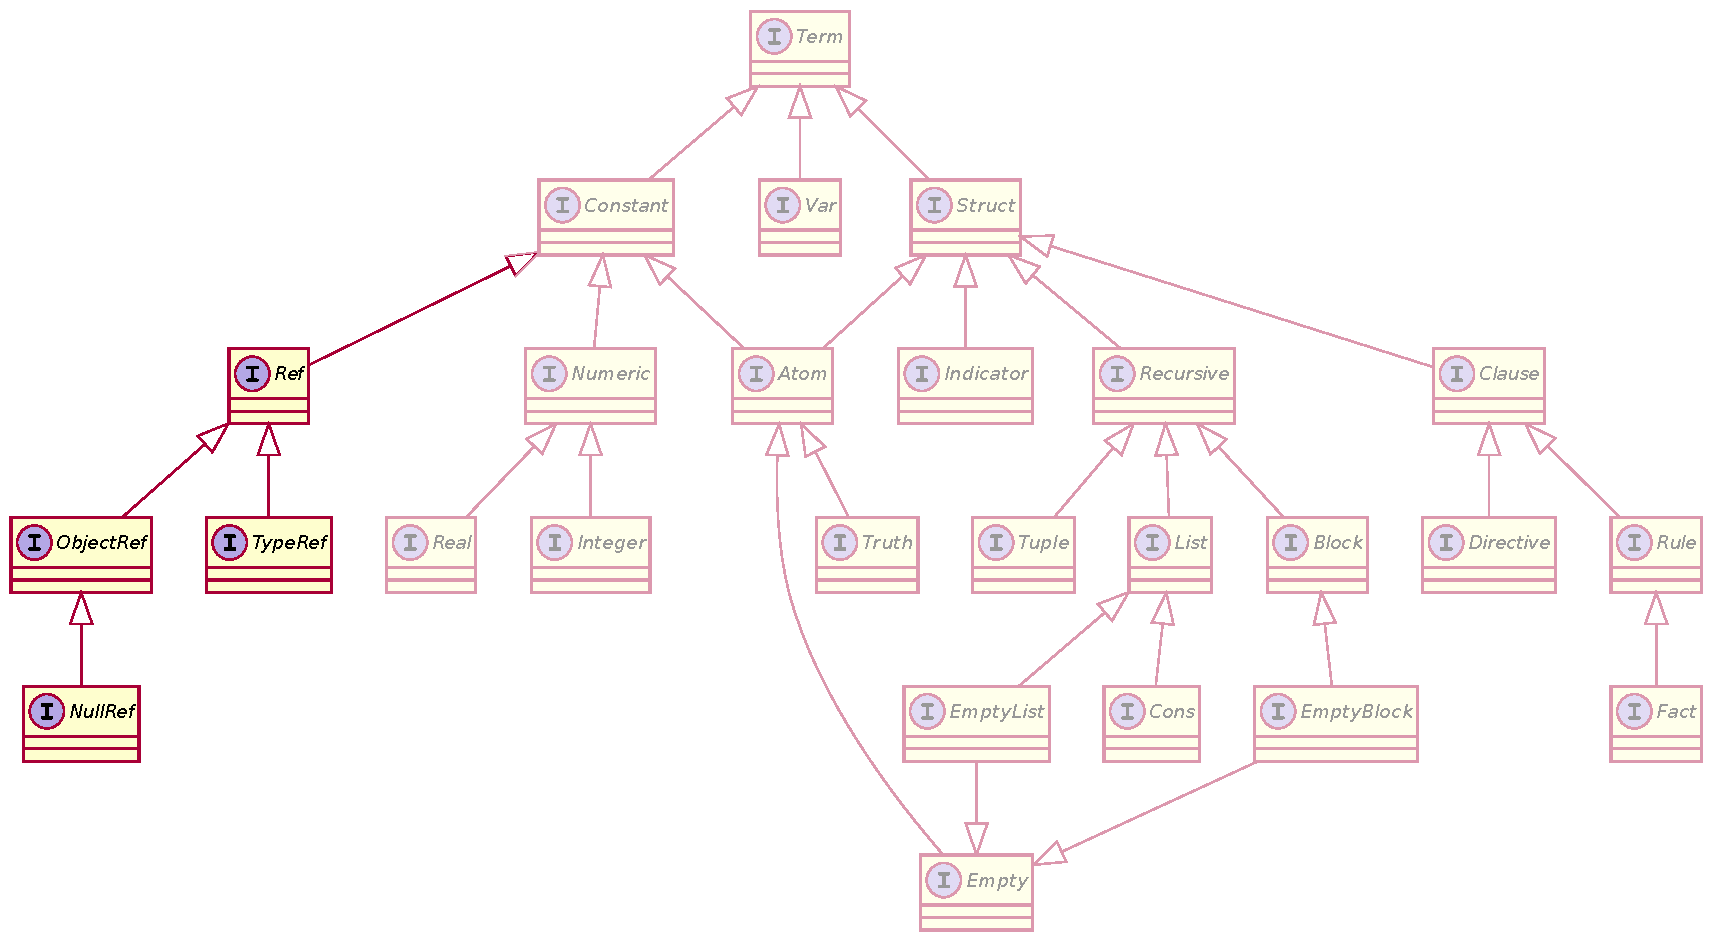
\includegraphics[width=0.8\linewidth]{figures/terms.pdf}
    \caption{Reference terms and their localization within the \twopkt{} term hierarchy}
    \label{fig:terms}
\end{figure}

\twopkt{}'s \module{core} module provides knowledge representation facilities via terms and clauses.
%
This is achieved via a hierarchy of types -- namely, the ``term hierarchy'', depicted in \cref{fig:terms} --, supporting the representation of structured or clausal information, within the logic realm.

However, these abstractions alone are not sufficient to support LP--OOP interoperability, as they only support representation of knowledge in logic form.
%
In other words, ordinary logic-based knowledge representation can only represent terms (i.e. alphanumeric or numeric constants, data structures, or variables) or Horn clauses.
%
Objects and types from the OOP realm cannot be represented.

To overcome these issues, \twopkt{} comes with a \module{oop-lib} module extending the term hierarchy as shown in \cref{fig:terms}.
%
Briefly speaking, the extension consists of a new sort of constant term, namely \emph{references}---formally denoted by the \kt{Ref} type in the diagram.
%
Reference terms can either reference \emph{objects} (\kt{ObjectRef}) or types (\kt{Types})---as OOP languages may support both instance and shared (a.k.a. static) methods.
%
The \emph{null} reference (\kt{NullRef}) is a particular type of object reference denoting the lack of reference.

Thanks to reference terms, objects can be represented in the logic realm, and carried around as part of the resolution process.
%
Combined with the generators feature, this feature enables logic solvers to take objects into account during resolution.
%
As constant terms, references can be bound to variables, unified, and passed as arguments to predicates, in both verses.
%
Whenever an object must be created or manipulated, a logic solver may delegate the task to the OOP realm, via some \emph{ad-hoc} generator.

Notably, this mechanism as well is fundamental to support the manipulation of schemas, datasets, transformations, and predictors in the \mllib{}.

\subsection{Selecting the underlying OO library}

Here we present a technological analysis aimed at selecting the most adequate library to support our \mllib{}.
%
The analysis is subject to a unique -- yet very strong -- constraint, derived from the nature of \twopkt{}: JVM compatibility.

Notably, \twopkt{} offers unique features which can hardly be found in other LP ecosystems.
%
These include the possibility
%
\begin{inlinelist}
    \item to exploit LP facilities \emph{as a library} in OOP,
    \item to define custom sorts of terms, and
    \item to implement custom logic predicates via OOP.
\end{inlinelist}
%
Unfortunately, however, these possibilities come at a price.
%
Any piece of OOP code willing to interoperate with \twopkt{} must be compliant with some of the platforms \twopkt{} supports---which currently means the JVM, JS, and Android.
%
Of these the JS platform is considered poorly adequate for ML -- as it is a platform mostly suited for Web-related solution --, while Android is too narrow---as targeting Android alone would imply the \mllib{} to only be usable on smart devices.
%
Ad-hoc native bindings towards C/C++ based solution for ML could be considered, but they would involve high costs in terms of engineering and maintenance---which would be prohibitive for and early research project.

Hence, in the reminder of this subsection we focus on JVM-based solutions for ML, supporting all the sorts of entities described in the previous sections---namely, Schemas, Datasets, Transformations, Predictors, and, in particular, Neural Networks.

\paragraph{\deeplearningforj{} (\dlfj)}

\dlfj~\cite{DL4J} is a Java-based solution for neural networks and deep learning, inspired to Python-based projects such as Tensorflow and Pytorch.

The project is currently developed and maintained by the Konduit team\footnote{\url{https://konduit.ai}}, and supported by the Eclipse Foundation\footnote{\url{https://www.eclipse.org}}.
%è un framework in Java e Scala per di applicazioni di Deep Learning su JVM.
%
%Il progetto è sviluppato da Konduit e supportato da Eclipse Fundation.
%
The project comes with a wide gamma of functionalities covering the many needs of the deep learning practitioner.
%
These include ND4J, i.e. an efficient library for tensors manipulation and scientific computations; Datavec, i.e. a library for loading data from various sources into tensors; Samediff, i.e. a Tensorflow/Pytorch-like differential engine for the execution and optimization of complex computational graphs; and Arbiter, i.e. a tool for hyper-parameters optimization.
%Il progetto offre un'ottima copertura di funzionalità attraverso una divisione in componenti dedicati alle diverse necessità di un programma di Deep Learning tra cui: ND4J per calcolo scientifico e algebra lineare con implementazioni ottimizzate per operazioni matematiche in larga scala, DL4J per costruzione e utilizzo di varie tipologie di reti neurali, Datavec per elaborazione e gestione di dati,astrazione di dataset e supporto a vari formati e Arbiter per l'ottimizzazione di iperparametri.

In particular, the Samediff engine is explicitly designed to rely on ND4J, thus guaranteeing good performance in spite of low memory requirements.
%Il motore differenziale Samediff è implementato come componente di ND4J ed è progettato per avere un buon rendimento con un utilizzo minimale della memoria.
%
Overall, \dlfj{} is interoperable with a number of relevant technologies from the ML playground, including but not limited to Spark (for the execution of distributed learning pipelines), CUDA (for hardware accelerating tensor manipulations), Tensorflow (as it supports the `\texttt{.h5}' data format), as well as the Open Neural Network Exchange (ONNX) format.
%Il framework è compatibile con spark e CUDA e supporta il formato '.h5' garantendo una forma di compatibilità con tensorflow.
%
Furthermore, \dlfj{} is shipped with a number of pre-trained models (model zoo), and many code snippets exemplifying their usage.
%In aggiunta alle librarie sono disponibili modelli pre-addestrati (Model Zoo) e una buona quantità di codice d'esempio.

The project is actively maintained and rapidly evolving.
%
It currently includes 56 contributors and more than 12.3k stars on GitHub.
%Il progetto è mantenuto e in crescita con frequenti aggiornamenti e conta 43 contributori e più di 11000 stelle su GitHub.
%
Its codebase is well documented on the project homepage, and several tutorials are provided as well.
%
Finally, \dlfj{} is an open source project made publicly available under the terms of the Apache 2.0 License.
%Il codice è ben documentato, e sono inoltre presenti diversi tutorial sul sito ufficiale. DL4J è disponibile con licenza ``Apache License 2.0''.


\paragraph{Smile}

Smile~\cite{SmileHomepage} is a Java-based solution for machine learning, inspired the Python-based project SciKit-learn.
%
It started as a side-project of dr. Haifeng Li., in 2014.
%
Nowadays, it is amongst the widest (in terms of features) independent frameworks for ML targeting the JVM platform.
%è un framework per applicazioni di Machine Learning su JVM scritto in Java e Scala, ed è un progetto indipendente di Haifeng Li, dottore di ricerca in Computer Science.
%
Notably, it does not simply support neural networks training and exploitation, but the whole gamma of ML predictors as well---including, but not limited to SVM, decision trees, linear models, random forests, etc.
%Attualmente supporta una larga varietà di algoritmi e modelli dell'ecosistema Machine Learning.
In particular, the Smile library includes pure-Java types and methods for linear algebra and tensor manipulation, dataset manipulation and visualization, and plenty of algorithms for both supervised and unsupervised ML, there including statistical methods, classification and regression, and a number of meta-heuristics.
%Il framework include una libreria per calcolo scientifico e algebra lineare, implementazione di diversi algoritmi e modelli per classificazione e regressione, supporto per apprendimento supervisionato e non supervisionato, metodi statistici e visualizzazione grafica di dati.

Unfortunately, NN support is very limited in Smile, as it only supports multi-layered percepts with dense layers, trained on the CPU---i.e. with no hardware acceleration.
%
Automatic differentiation support is lacking, as well as the possibility to construct custom network architectures.
%Una mancanza importante è però quella del supporto alle reti neurali a alla differenziazione automatica, questa componente è però citata in un ``Issue'' di GitHub come introduzione futura.
%

The project is actively maintained, mostly by dr. Li himself, and other 54 contributors, and it currently involves 5.4k stars on GitHub.
%Il progetto è periodicamente aggiornato e conta 43 contributori e più di 5000 stelle su Github.
%
Its codebase is well documented on the project homepage, and several tutorials are provided as well.
%Il progetto è ben documentato e sul sito ufficiale sono disponibili diversi tutorial rispetto alle singole componenti.
%
Finally, Smile is an open source project made publicly available under the terms of the Apache 2.0 License.
%Smile è disponibile con licenza `Apache License 2.0''

\paragraph{Neuroph}

Neuroph~\cite{Neuroph} is a Java framework for neural networks developed by at University of Belgrade through a number of PhD and master students' theses.
% è una framework Java che supporta le reti neurali, nato come parte di un progetto di tesi magistrale.
%
The project aims at providing a lightweight platform for exploiting and visualising neural networks, mostly in research and for teaching.
%Il progetto ha l'obbiettivo di fornire una piattaforma leggera e intuitiva da essere utilizzata principalmente a scopo didattico o di ricerca.

Similarly to other technologies presented so far, Neuroph supports the definition, training, assessment, and visualization of neural networks.
%
However, the amount of supported features is quite restricted, automatic differentiation is lacking, and the support for creating custom NN architectures is limited.
%Il framework supporta definizione, addestramento, valutazione e visualizzazione di reti neurali, tuttavia,in confronto ad esempio a DL4J o keras i metodi forniti sono semplificati, e sono presenti una minor varietà di tipologie di reti.
%
%La libreria inoltre non contiene un vero e proprio motore differenziale, delegando il calcolo differenziale al oggetto neurone, e non è quindi possibile definire un grafo computazionale.
%
These limitations are coherent with the design goal of creating a didactic environment for neural networks newbies, yet they may result prohibitive for complex projects needing to be competitive w.r.t. the state of the art.
%Queste semplificazioni sono coerenti con la scelta di creare uno strumento che consenta un primo approccio di uno studente con il Deep Learning, ma risultano essere limitanti per applicazioni in ambiti industriali o progetti di maggiore complessità.

The project is currently being maintained by Zoran Sevarac and other 21 contributors, and it currently involves 51 stars on GitHub.
%Il progetto è attualmente mantenuto e cita come autore principale Zoran Sevarac, conta 22 contributori e 40 stelle su GitHub.
%
Finally, Neuroph is an open source project made publicly available under the terms of the Apache 2.0 License, since version 2.4, or the LGPL license before that version.


\paragraph{Tensorflow for Java (TF4J)}

Tensorflow~\cite{tensorflow2015-whitepaper} is a popular framework for ML, and in particular deep learning developed by the Google Brain team.
%
It consists of a differential engine written in C++ and involving several bindings towards high-level languages, such as Python.

%è un popolare framework per Machine Learning e un motore differenziale per Python sviluppato da `Google Brain Team`.
%
TF4J is the official binding of Tensorflow for the JVM.
%è il progetto ufficiale di \emph{porting} su JVM.
Unfortunately, however, TF4J does not currently have the same maturity of the Python binding, nor it covers the same gamma of features.
%
Notably, TF4J does not support the support the whole API described by the official Tensorflow documentation.
%
In particular it does not support all the features introduced in Tensorflow 2.0, such as the Keras API---supporting the manipulation of NN in terms of layers.

%Il progetto conta 200 stelle su Github e 64 contributori.
The project involves more than 450 stars and 64 contributors on GitHub.
%
It consists of an open source project made publicly available under the terms of the Apache 2.0 License.

\paragraph{Deep Java Library (DJL)}

DJL~\cite{DJL} is a Java framework for deep learning application developed by Amazon.
%
%è un framework scritto in Java per applicazioni di Deep Learning su JVM sviluppato da Amazon Web Services.
%
It supports the definition, training, and exploitation of neural network, via one or more pluggable differential engines
%
%Il progetto propone una libreria per definizione, addestramento e utilizzo di reti neurali che sia agnostica rispetto alla scelta del motore differenziale.
The currently available differential engines are the Pytorch, MXNet, and Tensorflow ones.
%
For all such engines, a number of pre-trained neural architectures (model zoos) are provided as well.
%All'interno del framework sono inoltre presenti implementazioni per JVM dei motori differenziali di PyTorch, MXNet e ONNX e una libreria che incapsula TensorFlow, per ognuno di questi motori sono inoltre proposti vari modelli pre-addestrati.
%
Hence, DJL essentially consists of a common API for training or loading, and running NN targetting state of the art differential engines.
%Il progetto fornisce quindi una libreria comune a prescindere dalla scelta del motore differenziale e una piattaforma in cui poter utilizzare modelli recuperati da altri progetti.

Despite DJL is currently actively maintained, it is to be considered in embryonic stage.
%
At the time of writing, it mostly focuses on image processing and computer vision applications, while it does not include functionalities for handling datasets and their schemas.
%è regolarmente aggiornato ma ancora in una fase acerba dello sviluppo, le funzionalità offerte al momento sono incentrate sulla elaborazione di immagini e computer vision mentre non è presente una libreria per la gestione di dati in forma tabulare.

The project currently involves 48 contributors and 2.4k stars on GitHub.
%
It consists of an open source project made publicly available under the terms of the Apache 2.0 License.

\paragraph{H2O}

H2O~\cite{H2O} is a ML, deep learning, and distributed computing platform for the JVM, developed by H2O.ai.
%
%
%è una piattaforma per Machine Learning,Deep Learning e calcolo statistico su dati distribuiti, sviluppata da H20.ai.
It consists of a JVM-based service running on top of a cluster of machines, possibly involving Spark or Hadoop.
%
Clients may perform ML or data processing via a ReSTful API exposed by that service.
%
Implementations for that API are available for the R, Python, and JS languages.
%
%H20 prevede una componente server scritta in Java eseguibile su un cluster di nodi o su piattaforme come Spark o Hadoop che si interfaccia ai client tramite REST API, sono fornite implementazioni di client per R, Python e Web Browser.
%
%possono essere client applicazioni JavaScript, R, Python, Tableau o Web Browser Il server si occupa di gestire i dati distribuiti rappresentati in formato chiave-valore e di eseguire su di essi le computazioni richieste dai client, i vari algoritmi sono realizzati secondo il modello computazionale Map Reduce.
Clients may request data processing or ML operations on data, to the service, which then exploits the joint computational power of the cluster to perform those operations, following the map-reduce approach \cite{DeanG08}.
%
Hence, H2O is a nice solution for Big Data scenarios.
%H2O è quindi una soluzione interessante per applicazioni in ambito Big Data.

The project is actively maintained and it involves 154 contributors and 5.7k stars on GitHub.
%
%Il progetto è regolarmente aggiornato e conta 138 contributori e più di 5000 stelle du GitHub.
%
It consists of an open source project made publicly available under the terms of the Apache 2.0 License.
%H20 è disponibile con licenza ``Apache License 2.0``

\paragraph{Weka}

Weka~\cite{WittenFH11} is a platform for ML, and, in particular data mining, developed in Java by the Waikato University.
%è una piattaforma per Machine Learning, disponibile anche come libreria Java sviluppata della Università di Waikato.
%
It includes a wide collection of algorithms supporting not only supervised and unsupervised learning, but also data pre-processing, exploration, and visualization.
%
Weka can be exploited as a Java library or as a graphical application for data mining.
%
In the latter case, no coding skills are required for using Weka.
%Weka fornisce supporto a un vasta tipologie di applicazioni di Machine Learning quali elaborazione dati, apprendimento supervisionato e non supervisionato, analisi di modelli e altri.

Concerning NN, Weka provides basic support for multi-layer perceptrons only, without relying on automatic optimization.
%
Hence, the construction of arbitrarily-structured NN is not supported directly, but rather via the WekaDeepLearning4J extension\footnotemark---which wraps \dlfj{} behind the scenes.
%
\footnotetext{\url{https://deeplearning.cms.waikato.ac.nz}}
%Per quanto riguarda le reti neurali Weka ha recentemente introdotto un package dedicato denominato WekaDeepLearning4J, che come supponibile dal nome è basato su DeepLearning4J.

Weka is a well-established and widely-adopted solution within the data mining community.
%
The official Web page includes and excellent documentation, including tutorials and videos.
%è progetto completo e ampiamente diffuso nella comunità di sviluppatori, il sito principale contiene una ricca documentazione e video corsi.
%
It consists of an open source project made publicly available under the terms of the GPL 3.0 License.

\subsubsection{Comparison, discussion, and selection}

\begin{table}
    \begin{adjustbox}{width=\textwidth,center}
        \begin{tabular}{c||c|c|c|c}
            \textbf{Project} & \textbf{Developer / Funder} & \textbf{Maturity} & \textbf{Development Status} & \textbf{Documentation}
            \\\hline\hline
            \dlfj{} & Konduit/Eclipse Fundation & Beta & Actively Developed & Excellent
            \\\hline
            Smile & Haifeng Li & Stable & Developed & Excellent
            \\\hline
            Neuroph & Zorac Severac & Stable & Maintained & Acceptable
            \\\hline
            TF4J & Google Brain Team & WIP & Developed & Excellent
            \\\hline
            DJL & Amazon Web Services & Alpha & Actively Developed & Good
            \\\hline
            H20 & H20.ai & Stable & Developed & Good
            \\\hline
            Weka & Waikato University & Stable & Developed & Excellent
        \end{tabular}
    \end{adjustbox}
    \caption{Recap of the analysed technologies and their features}
    \label{tab:tech-features}
\end{table}

\begin{table}
    \begin{adjustbox}{width=\textwidth,center}
        \begin{tabular}{ c||c|c|c|c|c }
            \textbf{Project} & \makecell{\textbf{Neural} \\ \textbf{networks}} & \makecell{\textbf{Linear} \\ \textbf{Algebra}} & \makecell{\textbf{Dataset} \\ \textbf{pre-processing}} & \makecell{\textbf{Other sorts} \\ \textbf{of predictors}} & \makecell{\textbf{Differential} \\ \textbf{engine}}
            \\\hline\hline
            \dlfj & Yes & Yes & Yes & No & Yes
            \\\hline
            Smile & No & Yes & Yes & Yes & No
            \\\hline
            Neuroph & Yes & No & No & No & No
            \\\hline
            TF4J & Yes & No & No & No & Yes
            \\\hline
            DJL & Yes & Yes & No & No & Yes
            \\\hline
            H20 & Yes & Yes & Yes & Yes & Unknown
            \\\hline
            Weka & Yes & Yes & Yes & Yes & via \dlfj
        \end{tabular}
    \end{adjustbox}
    \caption{Recap of the analysed technologies and the functionalities they support}
    \label{tab:tech-functionalities}
\end{table}

Here we motivate the choice of \dlfj{} as the underlying OO library supporting our first implementation of the \mllib{}.

The selection criterion leading our choice takes into account a number of aspects summarised in tables \ref{tab:tech-features} and \ref{tab:tech-functionalities}.
%
In particular, for each technology, we analyse some features aimed at assessing its usability, stability, and durability (from a software engineering perspective), other than which and how many functionalities it offers.

Functionalities are, of course, of primary importance.
%
For instance, we prioritize NN support via a differential engine, as that would enable great flexibility in the construction, training, and exploitation of NN of different shapes.
%
Functionalities supporting the loading and manipulation of datasets and their schemas are equally relevant.
%
Conversely, supporting the full gamma of ML predictors is a nice to have (but not strictly required) functionality.

Business oriented features are, however, of paramount importance as well.
%
Even in presence of all required functionalities, technologies involving a large development team, a big funding organization, a large user base, or a high-paced development/release history should be preferred---as they are less likely to be dismissed or become unmaintained in the future.
%
%È opportuno quindi definire come condizione necessaria la presenza di reti neurali e come aspetti da valutare secondariamente la qualità dell'API, il supporto a funzionalità di contorno, la maturità del progetto, la prospettiva di crescita e manutenzione e la compatibilità con 2P-Kt.

Along this line, \dlfj{} is the most adequate option.
%
Indeed, the project provides a sufficiently large functionality support, and it comes with a good documentation and encouraging expectations for what concerns its maintenance and future development---as it is backed by the Eclipse Foundation, and it has a large user base.
%
Furthermore, it comes with a well engineered object-oriented API, whose meta-model is close the one we adopted while designing the \mllib{}.
%A partire da queste considerazioni complessive DeepLearnign4J appare essere la scelta più adeguata, il progetto infatti si presenta ben documentato, con un buona garanzia sulla manutenzione e crescita data dal supporto di Eclipse FUndation dal ampio numero di adottanti, e soprattutto completo dal punto di vista delle funzionalità supportate con in particolare un ottimo supporto al elaborazione dati.
%
Smile covers a wide gamma of functionalities, but it is poorly suited for NN, and, in particular, it is an independent project with a small development team and a low-paced release rate.
%Smile nonostante sia un encomiabile lavoro indipendente e fornisca supporto completo su tutti gli aspetti di Machine Learning è purtroppo carente relativamente alle reti Neurali.
%
Neuroph is mainly suited for educational application, and it provides too simple API.
%
Furthermore, while it is currently maintained, it is not actively developed any more, and no major releases are expected in the future.
%Neuroph è mirato a un uso educazionale e presenta un'API troppo semplificata.
%
TF4J is still too embryonic and its API is too limited, at the moment, to serve the purpose of the \mllib{}.
%TF4J è un progetto alle fasi iniziali di sviluppo e che presenta un'API limitata al calcolo differenziale, che non supportano un uso ad alto livello delle reti.
%
DJL is a promising project -- both from the technical and business-oriented perspectives --, however it is currently better suited for use cases where NN trained elsewhere needs to be executed on the JVM.
%
Furthermore, it provides less functionalities than \dlfj{}, while serving similar purposes.
%DJL è un progetto con buone prospettive ma che per il momento sembra essere più adeguato per sviluppatori con necessità di riutilizzare modelli proveniente da altre piattaforme piuttosto che per chi volesse sviluppare un nuovo progetto in quanto in confronto a DL4J le funzionalità fornite sono inferiori.
%
H2O is an interesting solution, but its client-server architecture may greatly complicate the low level design and implementation of our \mllib{}, hence it is not considered adequate for bootstrapping a prototype.
%H20 è un progetto strutturato per la gestione di Big Data ed non è quindi adeguato ad essere integrato all'interno di 2P-kt.
%
Finally, Weka another perfect solution for backing our \mllib{}: it supports the full gamma of required functionalities, it has a large contributors list, it is well established, and it has a large user base.
%
The main reason why we prefer \dlfj{} over Weka is that the latter fully supports NN only through the former.
%
So, when prototyping our \mllib{} we choose to rely on simplest possible setting -- namely, vanilla \dlfj{} --, instead of an integrated solution involving Weka + WekaDeepLearning4J---which may however be pursued in the future.
%Weka è invece un progetto completo rispetto alle funzionalità cercate e ben integrabile, tuttavia data l'intenzione di sviluppare un prototipo incentrato sulle reti neurali si è scelto di limitare le dipendenze e di non inserire il livello di indirezione presente in WekaDeepLearning4J considerando che non tutte le funzionalità di DL4J potrebbero essere accessibili.
%
%È opportuno inoltre considerare che data la compatibilità presente tra DL4J e Weka, se necessario si potrà fare uso di quest'ultimo per eventuali estensioni del progetto e che quindi la scelta compiuta non risulta essere limitante.

\section{\mllib{} Examples}
\label{sec:examples}

Here we exemplify the usage of the \mllib{} to serve the purposes described in \cref{ssec:goals}.

From a LP perspective, our examples assume the existence of a logic solver/language exploiting some implementation of the \mllib{}.
%
For the sake of simplicity, we assume a Prolog solver is employed.
%
Hence, examples consists of Prolog scripts, possibly involving standard Prolog predicates.

From a ML perspective, our examples assume a very simple scenario where a neural-network classifier is trained on the well known Iris dataset\footnotemark.
%
The resulting NN is then exploited to write a simple hybrid predicate aimed at classifying unseen Iris instances.
%
\footnotetext{\url{https://archive.ics.uci.edu/ml/datasets/iris}}

\paragraph{Declarative ML}

\begin{figure}
    \prologimport[
        label={lst:dataset-loading},
        caption={Dataset loading from file}
    ]{listings/dataset-loading.pl}
    %
    \prologimport[
        label={lst:pre-processing-pipeline},
        caption={Pre-processing pipeline}
    ]{listings/pre-processing-pipeline.pl}
    %
    \prologimport[
        label={lst:neural-network-declare},
        caption={Neural network structure declaration}
    ]{listings/neural-network-declare.pl}
\end{figure}

Declarativity is a key benefit of our symbolic approach to ML.
%
The \mllib{} supports declarative ML in several ways, as exemplified by listings \ref{lst:dataset-loading}, \ref{lst:pre-processing-pipeline}, \ref{lst:neural-network-declare}, and \ref{lst:training}.

In particular, \cref{lst:dataset-loading} shows how the schema and data entries of the Iris dataset can be treated in logic.
%
Notably, the Iris data set contains 150 rows describing as many individuals of the Iris flower.
%
For each exemplary, 4 continuous input attributes -- \emph{petal} and \emph{sepal width} and \emph{length} -- are recorded, other than a categorical target attribute---denoting the actual Iris \emph{species}.
%
There are three particular species of Iris in this data set -- namely, Setosa, Virginica, and Versicolor --, and the 150 examples are evenly distributed among them---i.e., there are 50 instances for each class.
%
The Prolog script describes the Iris dataset's schema in clausal form, as discussed in \cref{ssec:schemas}.
%
It also declares two predicates -- namely, \pl{iris\_schema/1} and \pl{iris\_dataset/1} -- aimed at letting the logic programmer retrieve either the schema or its dataset in object form.
%
More precisely, \pl{iris\_schema/1} attempts to read the schema from the local theory, while \pl{iris\_dataset/1} attempts the load the dataset from a CSV file.
%
\Cref{lst:logic-dataset-loading} (presented later in this section) reports a similar scenario where the dataset as well is loaded from the local theory.

\Cref{lst:pre-processing-pipeline} exemplifies the declaration of a pre-processing pipeline aimed at normalising the input attributes of any \pl{Dataset} having the same \pl{Schema} of Iris, other than one-hot encoding its output attributes.
%
The resulting \pl{Pipeline} is then fitted against the provided \pl{Dataset}, and bound to the corresponding output argument.

In turn, \Cref{lst:neural-network-declare} presents a general purpose predicate aimed at defining multi-layered perceptron predictors with an arbitrary amount of hidden layers.
%
This is made possible by the \pl{multi\_layer\_perceptron/4} predicate, which requires the caller to provide the amount of neurons to be instantiated for
%
\begin{inlinelist}
    \item the input layer (\pl{Nin}),
    \item the output layer (\pl{Nout}), and
    \item for each hidden layer (\pl{Nhidden}).
\end{inlinelist}
%
Notably, \pl{Nhidden} should consist of a list in integers, denoting the amount of neurons for each hidden layer -- from the outermost to the innermost --, while the total amount of integers corresponds to the amount of hidden layers.
%
The resulting neural network predictor is then bound to the \pl{NN} output argument.
%
So, for instance, a NN such as the one depicted in \cref{fig:mlp} can be declared as follows:
%
\begin{center}
    \pl{multi\_layer\_perceptron(4, [5, 7], 3, NN)}
\end{center}

Finally, \cref{lst:training} declares an end-to-end ML workflow aimed at selecting and training the best NN architecture to tackle Iris classification.
%
Further details about that listing are discussed later in this section.
%
For the moment, we simply stress the declarative nature of the script which can be regarded as a formal -- yet human-readable -- specification of a classifier training workflow.

\begin{figure}
    \centering
    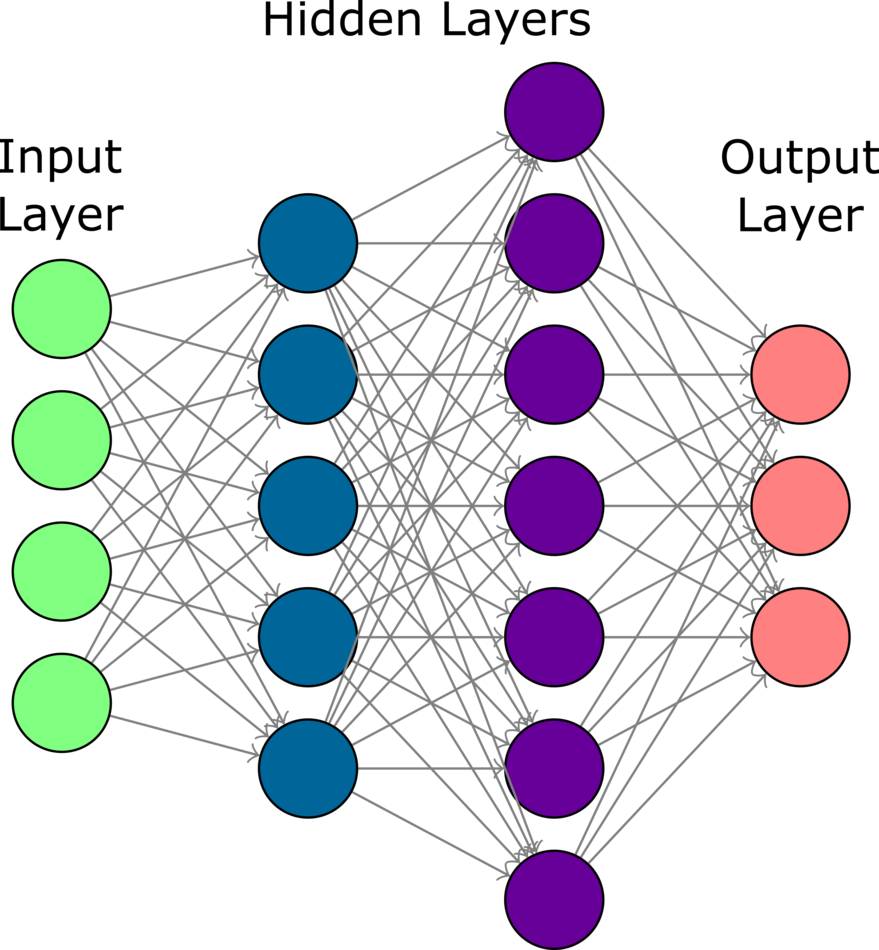
\includegraphics[width=.3\linewidth]{figures/mlp.png}
    \caption[Simplified representation of a multi-layer perceptron]{Simplified representation of a multi-layer perceptron having 4 input neurons, 2 hidden layers with 5 and 7 neurons respectively, and 3 output neurons}
    \label{fig:mlp}
\end{figure}

\paragraph{Symbolic data sources}

\prologimport[
    float,
    label={lst:logic-dataset-loading},
    caption={Dataset loading from the local theory}
]{listings/logic-dataset-loading.pl}

In an hybrid system integrating both symbolic reasoning and sub-symbolic learning, it may be useful to perform ML upon data expressed in logic form.
%
This requires logic theories to act as symbolic data sources.

Our \mllib{} makes it possible to support such scenario, as exemplified in \cref{lst:logic-dataset-loading}.
%
The script is assumed to replace \cref{lst:logic-dataset-loading} in those situation where the Iris dataset is logically described in clausal form.
%
Here, the \pl{iris\_dataset/1} attempts to load the data from the local theory instead of a file.

\paragraph{Model selection via resolution}

\prologimport[
    float,
    label={lst:training},
    caption={[Declarative description of a ML workflow]Declarative description of a ML workflow aimed at selecting the best hyper and learning parameters for a NN classifier. Ancillary predicates invoked in this snippet are reported in \cref{lst:training-ancillary}}
]{listings/training.pl}

\prologimport[
    float,
    label={lst:training-ancillary},
    caption={[Ancillary predicates used in \cref{lst:training}]Ancillary predicates used in \cref{lst:training}. Each predicate denotes one particular step of a model selection workflow}
]{listings/training-ancillary.pl}

The automatic exploration of a search space subtended by logic resolution could be exploited to perform model selection.
%
Indeed, model selection essentially consists of an exploration of the hyper and learning parameters space, looking for the best possible values---i.e. those hyper and learning parameters assignments corresponding to well-performing predictors on the available training set.

Accordingly, the \mllib{} supports expressing and performing model selection in logic, as exemplified in \cref{lst:training}.
%
There hyper, learning, and workflow parameters are expressed as logic facts, and the \pl{params/2} predicate is defined to enumerate all possible combinations of theirs---e.g. via Prolog's backtracking mechanism.
%
The \pl{model\_selection/5} predicate is in charge of stepping through all such parameters with the purpose of selecting, and training all corresponding NN predictors which attain a sufficiently high predictive performance---denoted by the \pl{target\_performance/1} fact.
%
For each trained predictor, the predicate outputs not only a reference to the \pl{Predictor} itself, but also its \pl{Performance}, and the affine \pl{Transformation} to be applied to each datum for which predictions should be drawn using that predictor.

More precisely, the predicate \pl{model\_selection/5} works by
%
\begin{enumerate}
    \item splitting the provided \pl{Dataset} into a \pl{TrainingSet} and a \pl{TestSet}, according to a split ratio (\pl{R}) declared by the \pl{test\_percentage/1} fact
    \item declaring and fitting a pre-processing \pl{Transformation} aimed at normalising the \pl{TrainingSet}'s input attributes, and one-hot encoding its output attributes
    \item applying such \pl{Transformation} to the \pl{TrainingSet}, hence producing
    \\
    a \pl{ProcessedTrainingSet}
    \item stepping through all possible hyper (\pl{HyperParams}) and learning (\pl{LearnParams}) parameters combinations,
    \item training each corresponding predictor, via 10-fold cross validation (CV), and computing its average validation-test performance (\pl{P})
    \item skipping each hyper and learning parameters combination such that the average performance \pl{P} is lower than the target performance \pl{T}
    \item re-training a full-fledged MLP on the whole \pl{TrainingSet}, for each parameters combination such that \pl{P >= T}
    \item testing that MLP against the \pl{ProcessedTestSet} -- attained by applying the aforementioned \pl{Transformation} to the \pl{TestSet} as well --, thus computing the MLP actual \pl{Performance}
\end{enumerate}
%
In other words, the \pl{model\_selection/5} represents a declarative, and pretty general, workflow for model selection---which may be adapted to other supervised learning tasks with minimal changes.
%
It relies on a number of ancillary predicates declaring some particular steps of the workflow, and exemplifying many \mllib{} functionalities.
%
These are reported in \cref{lst:training-ancillary}.
%
For instance, \pl{train\_cv/4} is in charge of performing 10-fold CV on a given \pl{Dataset}, to assess a given \pl{HyperParams}--\pl{LearnParams} combination, to then compute the \pl{AveragePerformance} of the 10 predictors constructed in this way.
%
Each single fold of a \pl{K}-fold CV process is managed by the \pl{train\_cv\_fold/5} predicate, which in turn exploits \pl{train\_validate/5} predicate to train and validate each single predictor.
%
Finally, the \pl{test/3} predicate can be exploited to either test or validate a predictor depending on whether the test or validation set is provided as argument.

Under these hypotheses, a model selection workflow for the Iris dataset may be triggered via a concise logic query such as:
%
\begin{center}
    \pl{?- iris\_dataset(D), iris\_schema(S), model\_selection(D, S, P, \_, A).}
\end{center}
%
If all aspects of the model selection workflow are correctly declared, the query should provide multiple successful solutions corresponding to all trained predictors (\pl{P}) and their test-set accuracies (\pl{A}).

\paragraph{Hybrid reasoning}

\prologimport[
    float,
    label={lst:hybrid-predictor},
    caption={[Declaration of an hybrid predicate aimed at classifying Iris flowers]Exploitation of the NN classifier trained in \cref{lst:training} to create an hybrid predicate -- namely \pl{iris/5} -- aimed at classifying Iris flowers}
]{listings/hybrid-predictor.pl}

Finally, \cref{lst:hybrid-predictor} shows the exploitation of a trained NN predictor as a predicate aimed at classifying (possibly) unseen instances of the Iris flower.
%
The script serves a twofold purpose: it exemplifies the \mllib{} functionalities aimed at drawing predictions out of trained ML predictors, and, in particular, it provides an example of an \emph{hybrid} reasoner---where symbolic and sub-symbolic AI seamlessly interoperate.

The script assumes a fact of the form \pl{iris\_nn(N, T)} is available into the solver's KB, storing a reference to a trained NN predictor (\pl{N}) and to the affine transformation (\pl{T}) to be applied to each datum the predictor should be fed with.
%
Such assumption may be satisfied, in Prolog, by a query such as the following one:
%
\begin{center}
    \pl{?- iris\_dataset(D), iris\_schema(S), model\_selection(D, S, N, T, \_), !, assert(iris\_nn(N, T)).}
\end{center}
%
which selects and trains a single NN and stores it into the solver's dynamic KB.

Under such assumption, logic programmers may write an \pl{iris/5} predicate such as the one shown in \cref{lst:hybrid-predictor}.
%
The predicate allows the caller to classify Iris instances by triggering a previously trained NN, and by letting it draw predictions on the data row attained by composing the predicate's arguments---via the \pl{predict/3} predicate.
%
The prediction is then converted into a class constant -- via the \pl{classify/4} predicate --, which is in turn bound to the output parameter of \pl{iris/5}---namely \pl{Species}.

It is worth to be highlighted that, from the caller perspective, the \pl{iris/5} described so far is undistinguishable from a purely symbolic predicate serving the same purpose (i.e., Iris classification) and having the same name and arity---such as the one described in \cref{lst:symbolic-predictor}.

\prologimport[
    float,
    label={lst:symbolic-predictor},
    caption={[A purely symbolic classifier for Iris flowers]A purely symbolic classifier for Iris flowers, functionally equivalent to the hybrid one from \cref{lst:hybrid-predictor}}
]{listings/symbolic-predictor.pl}

%----------------------------------------------------------------------------------------

\section{Recap and Research Perspectives}
\label{sec:conclusions3}

In this chapter, we propose a logic API supporting the seamless integration of logic solvers with sub-symbolic AI, and, in particular neural-network-based supervised ML.

Stemming from a domain analysis aimed at identifying the major computational entities involved in a supervised ML workflow, we design our API in terms of computational entities and the operations/functionalities they should support.
%
We then reify our API into a set of logic predicates composing the \mllib{}---i.e., an abstract logic library which any goal-oriented solver may support, there including Prolog ones.
%
Both the syntax and the semantics of each single predicate are discussed, as part of the major contribution of this chapter.
%
Architectural and technological requirements are discussed as well.

Among the most relevant requirements, we stress the need of realising the \mllib{} as a façade towards some lower-level OOP library for ML.
%
Furthermore, to support the prototyping of our \mllib{} on top of the \twopkt{} logic ecosystem -- which technologically unifies the LP and OOP realms --, we also require the underlying OOP library for ML to be JVM-compliant.
%
Hence, we elaborate on a technological discussion aimed at selecting the most adequate JVM technology for ML.

Finally, we provide a number of usage examples aimed at showing the potential of the \mllib{}.
%
In particular, we discuss examples where our logic API supports \emph{declarative} ML (possibly from symbolic data sources), model selection via resolution, and hybrid reasoning.
%
Indeed, the \mllib{} enables the user to formally define ML workflows in a way which is both human- and machine-interpretable, focussing on what should be done, rather than how.

Hybrid reasoning, in particular, is the most relevant contribution of ours.
%
It consists in the seamless integration of logic and sub-symbolic AI at the functional level.
%
In fact, thanks to our \mllib{}, trained sub-symbolic predictors may be used in LP as ordinary predicates.

\paragraph{Research Perspectives}

In the future, we expect contributions to stem from our \mllib{} along two different research threads.
%
The first thread concerns the exploitation of the \mllib{} to create hybrid systems, where LP and ML are integrated in manifold ways.
%
This is made possible by our logic API for ML, which reduces the abstraction gap among LP and ML, as well as the \mllib, which lowers the technological barriers preventing the integration of symbolic and sub-symbolic AI.
%
The second thread concerns the extensions of the \mllib{}, which should be eventually delivered to cover currently unsupported functionalities---as well as other ML predictors than NN.

\chapter{Bridging LP and XAI}
\label{chap:psyke}

\mypapers{psyke-woa2021}

Artificial neural networks (ANN), support vector machines (SVM), and other data-driven predictors are nowadays among the most-used tools to face a wide range of different tasks involving machines learning (ML) from data \cite{rocha2012far}.
%
In all those cases, the learning activity consists of tuning the parameters of predefined algorithms in order to maximise their predictive capability w.r.t.\ the data at hand.

The major drawback of state-of-the-art ML algorithms is that they are inherently \emph{opaque}, meaning that they do not provide any intelligible representation of what they learn from data.
%
This is why most of those algorithms are considered as black boxes (BB) which only represent knowledge in a \emph{sub-symbolic} way.
%
Nevertheless, despite their sub-symbolic operation may prevent human users from understanding \emph{how} they work, BB -- and, in particular, ANN -- are being increasingly applied to support forecasting and decision making in many different fields -- including, but not limited to, marketing, customer/user profiling, social networks, predictive maintenance, etc. -- because of their unprecedented predictive performance.

There exist, however, critical applications where black-box predictions or recommendations are unacceptable: for instance,  healthcare, finance and law domains, or any other area of knowledge where decision making may affect critical aspects of human lives---e.g. health, wealth, freedom, etc.
%
In all those cases, it is of paramount importance to rely on \emph{explainable} predictions, recommendations, or suggestions, in order to let humans retain accountability and liability over the decision or choices they make.

%\note{Repetition starts here}
%
%Many strategies can be exploited to pursue the purpose of explainability~\cite{GuidottiMRTGP19}.
%%
%Some authors suggest for instance to \emph{only} rely on \emph{interpretable} algorithms~\cite{Rudin2019} -- such as generalised linear models, decision trees, etc. -- to obtain data-driven solutions that are explainable by construction.
%%
%However, this may hinder predictive performance in the general case, as it essentially cuts off most effective algorithms---e.g., ANN.
%%
%Another strategy consists of deriving \emph{post-hoc} explanations \cite{KENNY2021103459}, aimed at reverse-engineering the inner operation of a BB so as to make it explicit.
%%
%In this way, data scientists can keep using prediction-effective algorithms such as ANN, while still attaining high predictive performance.
%%
%The focus of this chapter is on the latter strategy.
%
%Symbolic knowledge extraction (SKE) is among the most promising means to derive \emph{post-hoc} explanations for sub-symbolic predictors.
%%
%Roughly speaking, the main idea behind SKE is to enable the construction of a \emph{symbolic} surrogate model mimicking the behaviour of a given predictor.
%%
%There, symbols may consist of intelligible knowledge, such as \emph{rule} lists or trees.
%%
%Such rules can then be exploited to either derive predictions or to better understand the behaviour of the original predictor.
%
%SKE has been applied, for instance, to credit-risk evaluation \cite{baesens2003using,baesens2001building,steiner2006using},  healthcare -- i.e., to make early breast cancer prognosis predictions \cite{franco2007early} and to help the diagnosis and discrimination among hepatobiliary disorders \cite{hayashi2000comparison} or other diseases and dysfunctions \cite{bologna1997three} --, credit card screening \cite{setiono2011rule}, intrusion detection systems \cite{hofmann2003rule}, and keyword extraction \cite{azcarraga2012keyword}.
%
%\note{Repetition ends here}
As further discussed in \cref{sec:knowledge-extraction}, in this thesis we commit to symbolic knowledge extraction (SKE) as the preferred means to derive \emph{post-hoc} explanations for sub-symbolic predictors.
%
However, despite the wide adoption of SKE, a unified and general-purpose software technology supporting it is currently lacking.
%
In other words, the burden of implementing SKE algorithms is currently on data scientists alone, who are likely to realise custom solutions on a per-need basis.
%
Other than producing inertia w.r.t.\ the adoption of SKE in modern data, such a lack of viable technologies is somewhat anachronistic in the data-driven AI era, where a plethora of libraries and frameworks are flourishing, targeting all major programming paradigms and platforms, and making state-of-the-art machine learning algorithms easily accessible to the general public---cf. SciKit-Learn\footnote{\vurl{https://scikit-learn.org/stable}} for Python, or Smile\footnote{\vurl{https://github.com/haifengl/smile}} for the Java Virtual Machine (JVM).

Accordingly, in this chapter we present the design of \psyke{}, a general-purpose Platform for Symbolic Knowledge Extraction aimed at filling the gap between the current state of the art of SKE and the available technology.
%
More precisely, \psyke{} is conceived as an open library where different sorts of knowledge extraction algorithms can be implemented, exploited, or compared.
%
\psyke{} supports rule extraction from both classifiers and regressors, and makes the extraction procedure as transparent as possible w.r.t.\ the underlying BB, depending on the particular extraction procedure at hand.
%
Notably, it also supports the extraction of first-order logic (FOL) clauses, with the twofold advantage of providing human- and machine-interpretable rules as output.
%
Rules can then be used as either an explanation for the original BB, or as a starting point for further symbolic computations.
%
\psyke{} is designed as a general framework that can be specialised on multiple runtimes and programming environments.
%
The technology currently comes along with two main implementations to enable SKE in two key domains:
%
\begin{inlinelist}
    \item the JVM implementation for the symbolic AI domain, and
    \item the Python implementation for the sub-symbolic AI domain.
\end{inlinelist}
%
SKE is one of the elements that act as a bridge between the two domains, as well as the production of logic programs \cite{lloyd1990computational,Nerode1996} as output---in particular expressed as Prolog programs \cite{ColmerauerR93}.

A number of experiments involving rule extraction on both classification and regression tasks -- performed on well-known public data sets -- are discussed to demonstrate the versatility of \psyke{}.
%
To this end, we run framework experiments against various BB predictors and perform a comparison between different extraction procedures applied to the same task.
%
The comparison takes into account the fidelity of the extracted rules (w.r.t.\ the original BB) and predictive performance w.r.t.\ the data.

Accordingly, the remainder of this chapter is organised as follows.
%
\Cref{sec:state} describes the state of the art for SKE as well as some background notion to fully understand the work.
%
\Cref{sec:psyke} presents the design of \psyke{}, while in \cref{sec:experiments} some use cases showing how \psyke{} can be exploited are reported.
%
Conclusions are drawn in \cref{sec:conclusions2}.

\section{State of the Art}\label{sec:state}

In this section we firstly overview the state of the art for symbolic knowledge extraction (\cref{ssec:extraction}).
%
Then, we delve into the details of a selection of extraction algorithms---namely, the ones \psyke{} implementation currently supports (\cref{ssec:classifiers}--\cref{ssec:generalpurpose}).
%
The algorithm selection is performed by keeping \emph{variety} (rather than exhaustivity) in mind, so as to demonstrate the operation and versatility of \psyke{}.
%
In particular, our aim is to exemplify the many application scenarios that a data scientist may meet---e.g., extraction from either classifiers or regressors, trained on either categorical or continuous data.

Finally, we briefly outline the currently-available software object-oriented frameworks for ML  (\cref{ssec:smile}).
%
The overview is meant to make the chapter self-contained, given that one of these frameworks provides \psyke{} with pure ML functionalities---in particular, the design of \psyke{} assumes basic classification or regression support to be available as a software library.

\subsection{Knowledge Extraction}\label{ssec:extraction}

According to \cite{agentbasedxai-aamas2020}, a computational system is considered \emph{interpretable} if human beings can easily understand its operation and outcomes.
%
The majority of modern ML predictors, however, sacrifice interpretability to enhance the predictive performance, thus becoming increasingly complex.
%
They do so by merely focusing on learning highly-predictive -- yet \emph{sub-symbolic} -- input-output relations from data, while neglecting any attempt to make such relations \emph{symbolic}, i.e., intelligible for human.
%
For this reason, ML algorithms are often called \emph{black boxes} \cite{Lipton18}.

To mitigate interpretability issues without sacrificing predictive performance, a number of authors from the \xai{} community have proposed means to produce \emph{ex-post} explanations for sub-symbolic predictors---most notably, ANN and SVM.
%
Explanations, in this case, consist of \emph{surrogate} predictors trained to mimic the ones to be explained, as closely as possible.

In practice, among the manifold proposals, some authors describe methods to extract if-then-else rules \cite{CravenS94,HuysmansBV2006,gridex-extraamas2021}, whereas others propose methods extracting decision trees \cite{CravenS95}.
%
While the shape of the extracted knowledge may vary from an extraction procedure to another, all the proposed methods share the trait of extracting \emph{symbolic} (i.e. human-intelligible) knowledge out of \emph{sub-symbolic} ML predictors.
%
Given a trained predictor and a knowledge-extraction procedure applicable to it, the extracted rules/trees act as \emph{explanations} for that predictor -- or as a basis to build some --, provided that they retain high \emph{fidelity} w.r.t.\ the underlying predictor \cite{agentbasedxai-aamas2020}.
%
The extracted knowledge may then enable further manipulations, such as merging the \emph{know-how} of two or more BB models \cite{xmas-aiiot2019}.

According to \cite{xaisurvey-ia14}, knowledge extraction methods can be categorised along three orthogonal dimensions, namely:
%
\begin{inlinelist}
    \item\label{item:category:learning-task} the sort of learning tasks they support,
    \item\label{item:category:knowledge-form} the shape of the symbolic knowledge they produce,
    \item\label{item:category:translucency} their \emph{translucency}---i.e., the sort of BB algorithms they can extract symbols from.
\end{inlinelist}

About dimension \ref{item:category:learning-task}, one can distinguish among algorithms targeting classification tasks, regression tasks, or both.
%
In other words, some extraction algorithms can only deal with BB classifiers -- e.g.\ Rule-extraction-as-learning~\cite{CravenS94} (\real, henceforth), \trepan~\cite{CravenS95} and others \cite{BarakatD2005,MartensBVGV2007} --, while others can only deal with BB regressors -- such as \iter~\cite{HuysmansBV2006}, \gridex~\cite{gridex-extraamas2021}, \textsc{RefAnn}~\cite{SetionoLZ2002}, \textsc{Ann-DT}~\cite{schmitz1999ann} and \textsc{RN2}~\cite{saito2002extracting} --, and only a few can handle both---such as \textsc{G-Rex}~\cite{grex-icdm2008} and \cart~\cite{breiman1984classification}.
%
Notably, virtually all extraction methods proposed so far are tailored on \emph{supervised} machine learning.
%
To the best of our knowledge, no rule extraction procedure has been proposed targetting unsupervised or reinforcement learning tasks.

As far as dimension \ref{item:category:knowledge-form} is concerned, decision rules \cite{freitas2014comprehensible,huysmans2011empirical,murphy1991id2} and trees \cite{quinlan1993c4,simplifyingdt-ijmms27} are the most widespread human-understandable shapes for extracted knowledge, thus most methods produce one of these two structures.
%
In both cases, decision rules or nodes are expressed in terms of the same input/output data types the original BB has been trained upon.
%
So, for instance, an extraction procedure processing a BB classifier for $N$-dimensional numerical data, over $K$ classes, will likely output rules/trees involving one or more \emph{predicates} over $N$ input variables $x_1, \ldots, x_n$ and $K$ possible outcomes.
%
In any case, however, extraction algorithms are further categorised w.r.t.\ the particular sort of predicates their output rules/trees may contain.
%
Accordingly, conjunctions/disjunctions of inequality (e.g.\ $x_i \gtrless c$), or interval inclusion/exclusion expressions (e.g.\ $x_i \in [l, u]$) are commonly exploited for numerical data, while equality (e.g.\ $x_i = c$) or set-inclusion $x_i \in \{c_1, c_2, \ldots \}$ expressions may be exploited for categorical data.
%
Finally, \mofn{} rules are yet another possible choice in the case of boolean data.

The translucency dimension \cite{AndrewsDT95} from \cref{item:category:translucency} refers to the need/capability of the extraction procedure to ``look into'' the \emph{internal} structure of the underlying BB---i.e., to what extent it has to be taken into account during the extraction procedure.
%
There are two major ways for categorising knowledge extractors w.r.t.\ translucency.
%
During the extraction process, \textit{decompositional} extractors may take into account the internal structure of the BB they operate upon, while \emph{pedagogical} ones do not.
%
For this reason, pedagogical approaches are usually more general -- despite potentially less precise --, thus they can be applied to every BB predictor regardless of its kind, structure, and complexity.

The quality of knowledge-extraction procedures is evaluated through different indicators depending on the task to solve, for instance, fidelity and predictive performance measurements \cite{towell1993extracting}.
%
In particular, the former indicates how well the extracted knowledge mimics the underlying black-box predictions, whereas the latter measures the explanator predictive power w.r.t.\ the data.
%
In all cases, measurements should be taken via the same scoring function used for assessing the BB performance---which in turn depends on the task it performs.
%
In the particular case of black-box classifiers, examples of performance measurements are accuracy, precision, recall, and F1-score; for BB regressors, the mean absolute/squared error (MAE/MSE) and the R${^2}$ scores could be exploited.

In the following, we provide a more detailed description of some extraction procedures currently supported in the \psyke{} framework, grouped by the task they address---i.e.\ classification, regression, or both of them.
%
All the algorithms are \emph{pedagogical}, thus they only rely on the BB inputs and outputs, and do not inspect the inner structure of the underlying BB.
%
This is why they can be applied to any kind of arbitrarily-complex BB.
%
In any case, structured data are required.
%
The same algorithms are summarised in \cref{tab:psyke}.

% !TeX root = ../phd-thesis.tex

\begin{table}
    \begin{adjustbox}{width=\linewidth}
    	\begin{tabular}{llllll}
    		\hline
    		Extraction Algorithm & Task & Translucency & Required Features & Knowledge Shape & Exhaustive \\
    		\hline\hline
    		\real{} & Classification & Pedagogical & Binary & Rule list & No \\
    		\trepan{} & Classification & Pedagogical & Binary & Decision tree  & Yes\\
    		\iter{} & Regression & Pedagogical & Continuous & Rule list & No \\
    		\gridex{} & Regression & Pedagogical & Continuous & Rule list & Yes \\
    		\cart{} & Classification & Pedagogical & Continuous & Decision tree & Yes \\
    		& and regression & & or binary & & \\
    		\hline
    	\end{tabular}
    \end{adjustbox}
    \smallskip
    \caption{Summary of the knowledge-extraction algorithms supported by \psyke{}}
    \label{tab:psyke}
\end{table}


\subsubsection{Extraction from Classifiers}\label{ssec:classifiers}

\paragraph{Rule-extraction-as-learning}\label{par:real}

\real{} \cite{CravenS94} is a pedagogical algorithm to extract conjunctive rules from trained BB classifiers by using a learning process driven by sampling and queries.
%
Output rules can be either \emph{if-then} or \mofn{} rules.
%
An example of \emph{if-then} output rule is the following: $\textit{Output class is} ~ C ~ \textit{if} ~ \{ \mathit{X}, \mathit{Y}, \mathit{Z} \} \allowbreak ~ \textit{are True} \allowbreak \textit{and} ~  \{ \mathit{U}, \mathit{V} \} ~ \textit{are False},$
%
\noindent where \textit{U, V, X, Y, Z} are one-hot encoded input features.
%
Such features are \textit{True} if they are 1, \textit{False} otherwise.

Output rules are disjunctive normal form expressions; each term is the conjunction of a data set feature subset, adequately generalised by dropping each non-discriminant antecedent.
%
\real{} cannot handle real-valued features, but only binary ones.

\paragraph{\trepan}\label{par:trepan}

\trepan{} \cite{CravenS95} is a pedagogical algorithm able to extract symbolic and comprehensible model representations from trained classifier BB by inducing a decision tree approximating the BB represented concept.
%
It usually maintains high fidelity levels w.r.t.\ the underlying BB while being comprehensible and accurate.
%
It is general in its applicability and well scalable with complex models or problems.
%
However, as \real{}, it cannot be applied to real-valued features.

In \cref{fig:trepanTree} an example of output tree is reported.
%
Internal nodes are represented by squares, while leaves are circles.
%
Variables reported inside the internal nodes are the split criteria for the subtree creation.
%
$C_i$ are the class labels corresponding to each leaf.

\begin{figure}
    \centering
    \begin{subfigure}{0.4\textwidth}
        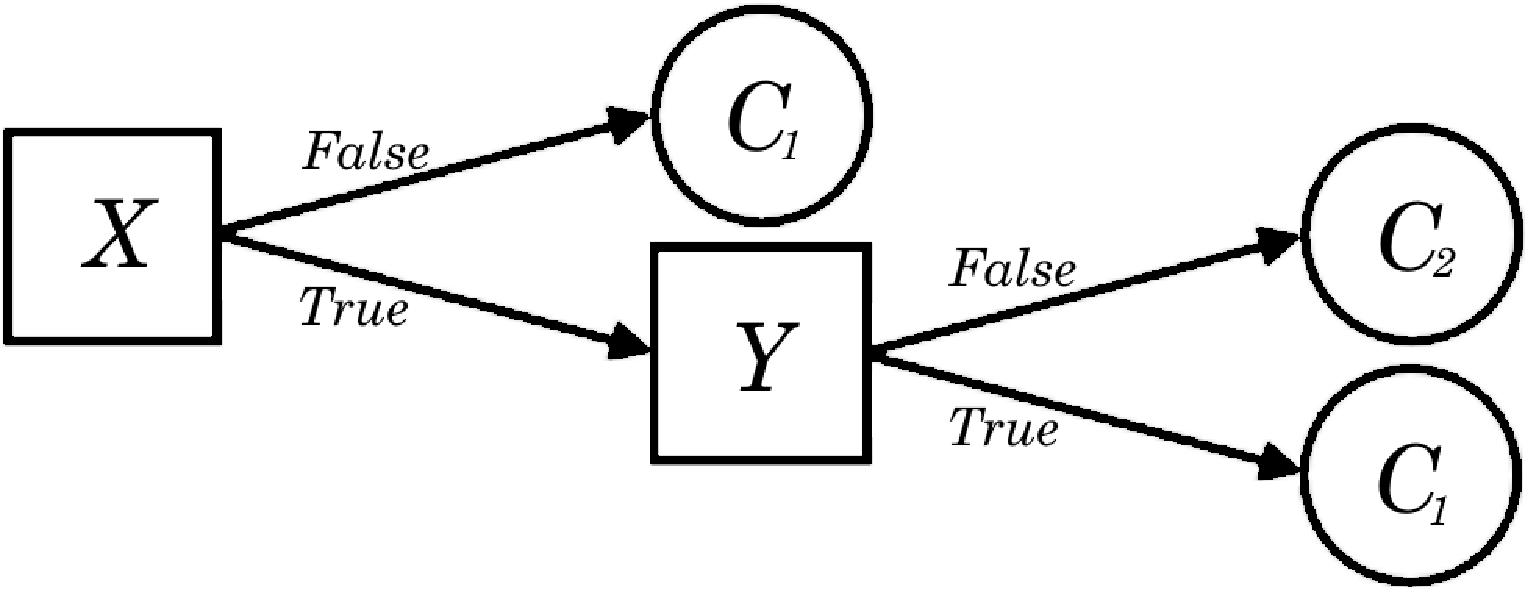
\includegraphics[width=\linewidth]{figures/tree.pdf}
    \end{subfigure}
    \hfill
    \vrule
    \hfill
    \begin{subfigure}{0.45\textwidth}
        \begin{align*}\footnotesize
            \begin{split}
                \text{Output} ~ & \text{class is} ~ C_1 ~ \text{if}
                \begin{cases}
                    ( \mathit{X} ~ \text{is \textit{True}} ) ~ \text{or}
                    \\
                    ( \mathit{X} ~ \text{is \textit{False} and} ~ \mathit{Y} \text{ is \textit{True}} )
                \end{cases}
                \\
                \text{Output} ~ & \text{class is} ~ C_2 ~ \text{otherwise.}
            \end{split}
        \end{align*}
    \end{subfigure}
    \caption{Example of \trepan{} output tree (left) and corresponding rules (right)}
    \label{fig:trepanTree}
\end{figure}

\subsubsection{Extraction from Regressors}\label{ssec:regressors}

\paragraph{\iter}\label{par:iter}

\iter{} \cite{HuysmansBV2006} is a pedagogical algorithm for building predictive rules from trained BB regressors of any kind.
%
Its main idea is to iteratively expand a number of hypercubes until they cover the whole input space.
%
Each of them is finally converted into an \emph{if-then} rule of the following format:
$\textit{Output} ~ \textit{constant is} ~ C ~ \textit{if} ~ X_1 \in [l_1, \mathit{u_1}]
~\textit{and} ~ ... ~ \textit{and} ~ \mathit{X_k} \in [\mathit{l_k}, \mathit{u_k}]$,
%
where $l_i$ and $u_i$ are the lower-bound and the upper-bound for variable $X_i$.
%
There, the preconditions of the rule describe a $k$-dimensional hypercube.
%
Indeed, \iter{} supports continuous input features, differently from the other algorithms presented so far.

\paragraph{\gridex}\label{par:gridex}

\gridex~\cite{gridex-extraamas2021} is another pedagogical extraction algorithm for regressors; it is an extension of \iter{} aimed at overcoming its major drawback: non-exhaustivity.
%
\gridex{} adopts a top-down approach to iteratively partition the input feature space in a user-defined number of hypercubes or in an automatic way accordingly to a user-defined strategy based on feature importance.
%
As \iter{}, \gridex{} produces \emph{if-then} rules and only accepts data sets with real-valued input features, but it is always exhaustive by design.
%
Since the procedure associates each hypercube to a rule, a merging phase is performed after every iteration as an optimisation to reduce the number of rules.

\subsubsection{General-Purpose Extractors}\label{ssec:generalpurpose}

\paragraph{\cart}\label{par:cart}

\cart{} \cite{breiman1984classification} is an algorithm for building decision trees that can be used to face both classification and regression tasks.
%
\cart{} is not properly a knowledge-extraction procedure, but from its output tree it is straightforward to obtain a rule tree, since each node of the \cart{} tree corresponds to a constraint on a certain feature and thus each path from the root to a leaf is a single complete classification or regression rule.
%
The algorithm can be summarised via the following instructions:
%
\begin{inlinelist}
    \item initialise the tree root node;
    \item find optimal splits and add new internal nodes and leaves accordingly;
    \item stop the algorithm based on one or more criteria---e.g., leaf number or tree depth.
\end{inlinelist}
%
Pruning algorithms can be applied to reduce the number of leaves.

\subsection[OOP Frameworks for ML]{Object-Oriented Programming Frameworks for ML}\label{ssec:smile}

\begin{figure}
    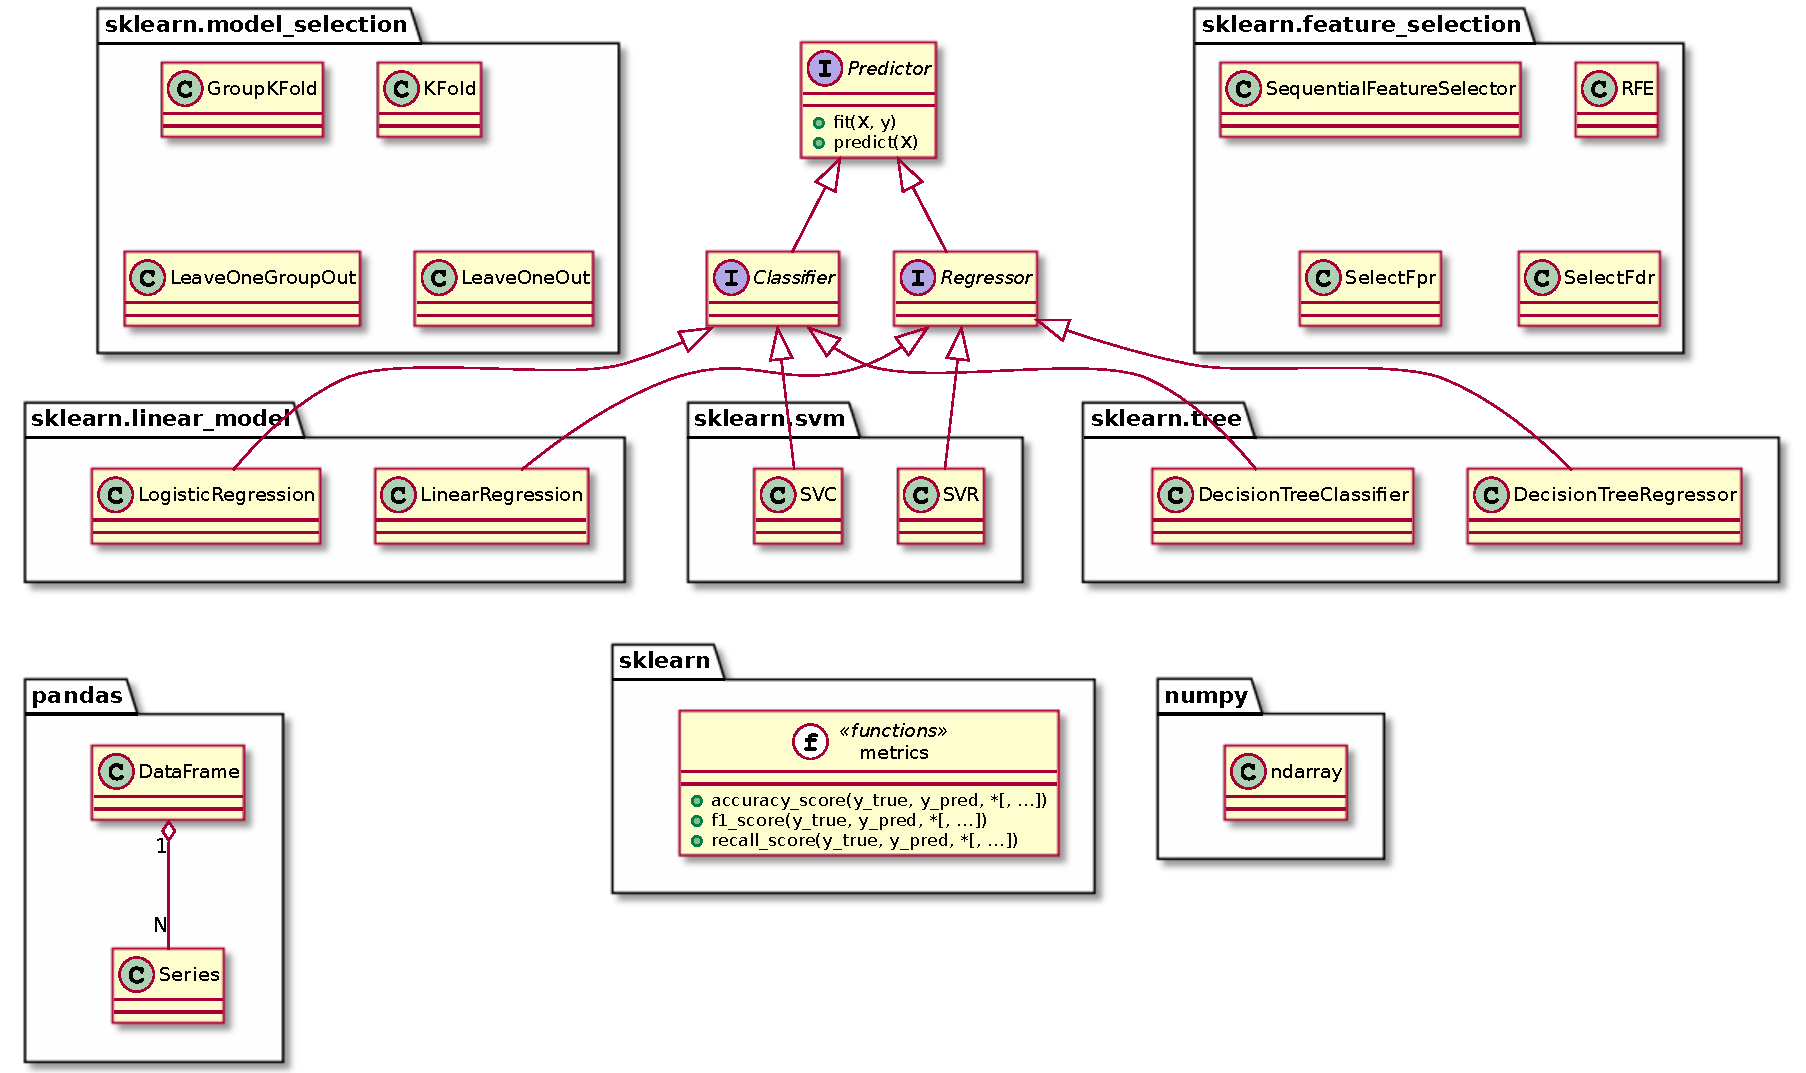
\includegraphics[width=\linewidth]{figures/scikit-simple.pdf}
    \caption{Overview on (a small portion of) the API of the \scikit{} library supporting classification and regression tasks}
    \label{fig:scikit}
\end{figure}

\begin{figure}
    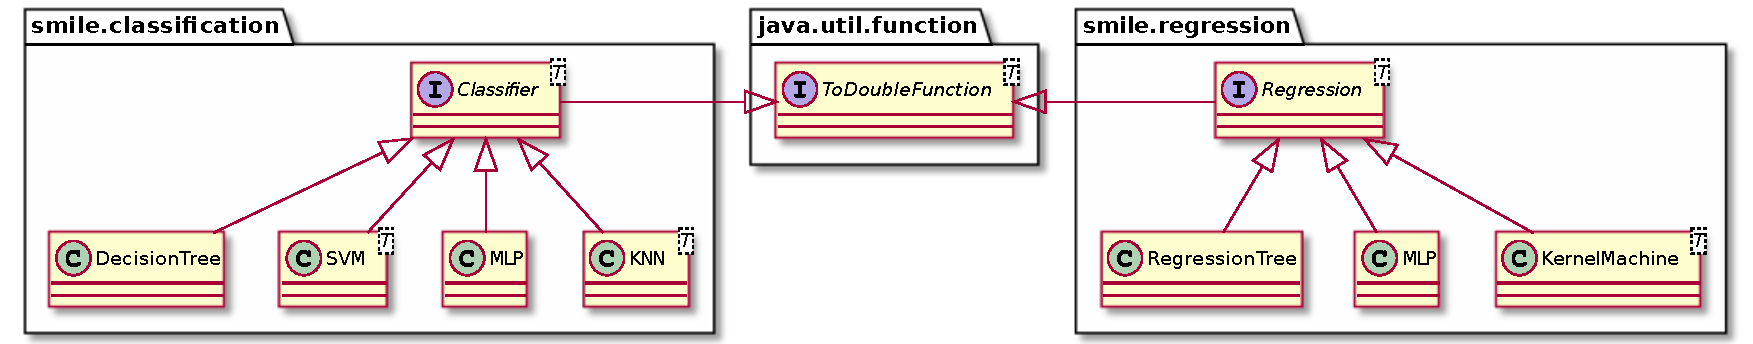
\includegraphics[width=\linewidth]{figures/smile-simple.pdf}
    \caption{Overview on the API of the \smile{} library supporting classification and regression tasks}
    \label{fig:smile}
\end{figure}

%\gcnote{Bisogna generalizzare questa sezione perchè dia il metamodello di \smile{} e \scikit{}, cogliendo analogie e differenze. È possibile entrare poi nel dettaglio delle tech, e quindi riusare del testo nella parte \smile{}-specific.}

In order to make ML solutions easily available, a number of frameworks -- especially exploiting object-oriented programming (OOP) -- have been developed.
%
Such frameworks usually provide users with powerful abstractions for modelling BB as well as for performing data set pre-processing, feature engineering and predictive performance measurements.
%
Among the most supported ML models, there are ANN, SVM, and decision trees for both classification and regression tasks.
%
The most complete frameworks also provide utility packages to ease the data set reading from (and writing into) files and to perform feature selection, beyond many other tools for natural language processing, linear algebra, and data visualisation.
%
Examples of state-of-the-art OOP frameworks for ML are \scikit{}~\cite{PedregosaVGMTGBPWDVPCBPD11} for Python and \smile{} \cite{SmileHomepage} for the JVM.

At the conceptual level, the design of such frameworks is similar, and similar are the set of functionalities they provide.
%
For this reason, the design of \psyke{} assumes an underlying ML framework to be available, from which major ML-related facilities can be borrowed.
%
In the general case, these facilities include:
%
\begin{enumerate}[label=\textbf{F\arabic{*}}]
    \item\label{facility:predictor-type} a base type for supervised predictors (i.e., either classifiers or regressors), providing a common interface for their training and their exploitation for inference;
    \item\label{facility:classifier-regressor-types} a base type for classifiers and a base type for regressors, as particular sub-sorts of predictor, providing a way to discern among the two at runtime;
    \item\label{facility:specific-predictor-types} \emph{ad-hoc} sub-types for well-known predictors -- such as ANN, SVM, decision trees, etc. --, encapsulating the algorithmic strategies for their training and their inference, and supporting the manipulation of individual predictors as instances of those types;
    \item\label{facility:dataset-schema-types} a type for representing data sets and their schemas, providing a common interface for their manipulation (scaling/translating columns, adding/removing features or instances, renaming/moving/transforming features, etc.);
    \item\label{facility:parametrisation} the possibility to parametrise predictors' training by letting developers specify hyper-parameters;
    \item\label{facility:scoring} the possibility to select one or more scoring functions to assess the performance of trained (or in-training) predictors;
    \item\label{facility:best-practices} support for ML best practices, such as test set separation, cross-validation, grid search, etc.;
    \item\label{facility:feature-engineering} support for feature engineering (there including selection, encoding, missing values imputation, etc.);
    \item\label{facility:inspection} the possibility to inspect the internals of any individual predictor (e.g. synapses in neural networks, or decision splits for decision trees, etc.), which is necessary to support the implementation of decompositional extraction algorithms.
\end{enumerate}
%
The abstract architecture of \psyke{} can be reified on each programming platform for which a library providing the facilities above exists.
%
Notably, in this chapter, we demonstrate the versatility of our design by describing two different implementations of \psyke{}.
%
One implementation is based on \scikit{} and targets Python, whereas the other is based on \smile{} and targets the JVM.

\subsubsection{\scikit{}}

\scikit{} \cite{PedregosaVGMTGBPWDVPCBPD11} is amongst the most well-known Python libraries for machine learning.
%
It is characterised by a coherent design, an efficient implementation and the wideness of its scope---which covers ML far beyond supervised techniques.

\Cref{fig:scikit} depicts a (partial) UML class diagram representing the major interfaces and classes composing \scikit's supervised learning API.
%
Module names are explicitly indicated to help the user understand the organisation of the library.
%
Notably, \scikit{} heavily rely on Python's \emph{duck typing} convention.
%
So, despite no explicit type definition exists for predictors (neither for classifiers nor for regressors) -- meaning that facility \cref{facility:classifier-regressor-types} is not supported --, all objects exposing the methods \py{fit(\ldots)} and \py{predict(\ldots)} are considered as such---approximating facility \cref{facility:predictor-type} via convention.
%
Nevertheless, each kind of ML predictor has a dedicated class (facility \cref{facility:specific-predictor-types}) and each class follows the aforementioned convention.
%
Parametrisation of learning (facility \cref{facility:parametrisation}) occurs at the instantiation level, via construction parameters.

External packages, such as Pandas\footnote{\vurl{https://pandas.pydata.org}} and Numpy\footnote{\vurl{https://numpy.org}}, provide data types for easily managing data sets, features, and tuples (intended as data set columns and rows, respectively).
%
The three Python packages -- \scikit, Pandas, and Numpy -- are independently maintained and deployed, despite being perfectly interoperable.
%
In particular, Numpy features efficient implementations for multi-dimensional arrays, while Pandas provides for higher-level abstraction such \py{DataFrame}s, for data sets, or \py{Series}, for both schemas and instances (facility \cref{facility:dataset-schema-types}).
%
Scoring functions (facility \ref{facility:scoring}) are reified as functions having analogous signatures (name apart), hosted by the \py{sklearn.metrics} module.
%
Conversely, cross-validation, grid search, and other model-selection tools (facility \cref{facility:best-practices}) are reified into \emph{ad-hoc} classes as well, hosted by the \py{sklearn.model\_selection} module.
%
Finally, feature extraction and selection (facility \cref{facility:feature-engineering}) are supported via the \kt{smile.feature\_ex\-trac\-tion} and \kt{smile.fea\-tu\-re\_se\-lec\-tion} modules, respectively, and the many classes therein contained.

Inspectability (facility \cref{facility:inspection}) can be achieved via Python ``consenting adults'' philosophy, which essentially allows expert programmers to freely access the internals of any Python object---there including \scikit{} predictors.
%
Therefore, decompositional extraction algorithms can be implemented on top of \scikit{}, provided that the inner functioning of predictors includes enough documentation to let programmers inspect them.

\subsubsection{\smile{}}

\smile{} (Statistical Machine Intelligence and Learning Engine) \cite{SmileHomepage} is defined as ``a fast and comprehensive machine learning engine'' for Java, and any other JVM-based language---e.g. Scala and Kotlin.

\Cref{fig:smile} depicts a (partial) UML class diagram representing the major interfaces and classes composing \smile{} supervised learning API.
%
Package names are explicitly indicated to avoid confusion between homonymous classes.
%
Notably, each kind of ML predictor has a dedicated class (facility \ref{facility:specific-predictor-types}) and each class implements either the \kotlin{Classifier} or the \kotlin{Regression} interface (facility \ref{facility:classifier-regressor-types}).
%
Both interfaces descend from the \kotlin{ToDoubleFunction} interface, which is, therefore, the most adequate type to represent any supervised ML predictor (facility \ref{facility:predictor-type}).
%
Parametrisation of learning (facility \ref{facility:parametrisation}) occurs at the instantiation level, via construction parameters.

Other packages (not shown in figure) provide data types for easily managing data sets, feature vectors, and tuples (intended as data set columns and rows, respectively) other than all the aforementioned facilities.
%
So, for instance, the \kotlin{DataFrame}, \kotlin{StructType}, and \kotlin{Tuple} types are the basic types for representing data sets, schemas, and instances, respectively (facility \ref{facility:dataset-schema-types}).
%
Scoring functions (facility \ref{facility:scoring}) are reified as classes as well, implementing either the \kotlin{ClassificationMetric} or the \kotlin{RegressionMetrics} interface.
%
A similar statement holds for cross-validation (facility \ref{facility:best-practices}).
%
Finally, feature engineering and selection (facility \ref{facility:feature-engineering}) are supported via the \kotlin{smile.feature} package and the many classes therein contained.

Inspectability (facility \ref{facility:inspection}) is apparently laying outside the current design goals of \smile{}: the current API of \smile{} does not provide any means to observe the internals of trained predictors.
%
Therefore, only pedagogical extraction algorithms can be implemented on top of \smile{}.

\section{\psyke}\label{sec:psyke}

\begin{figure}
    \centering
    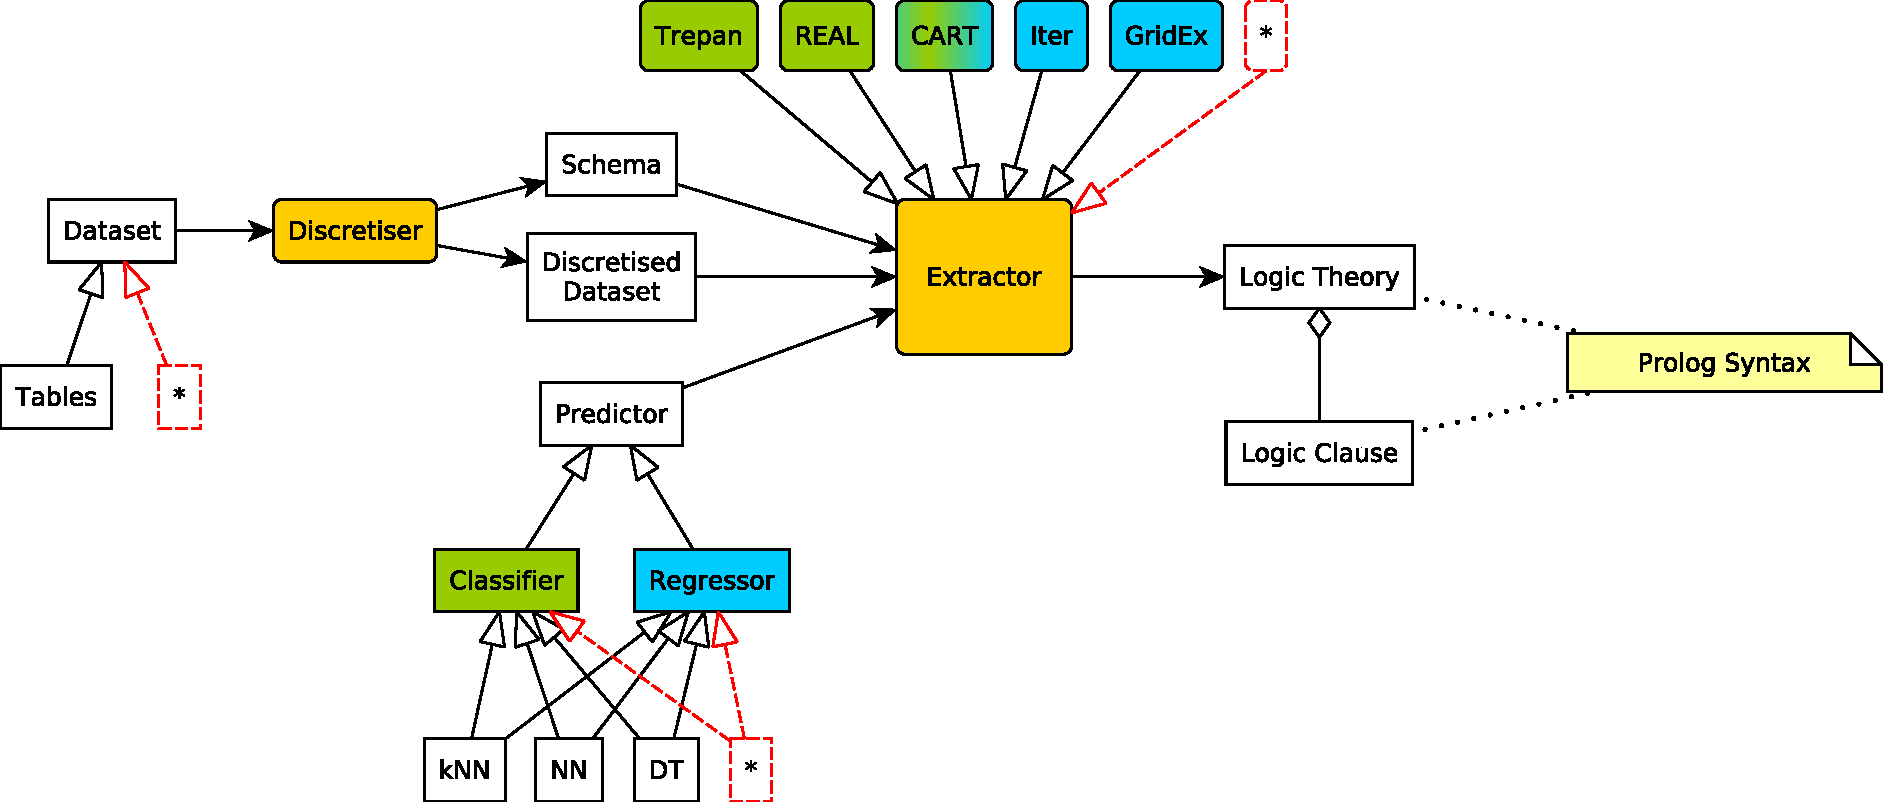
\includegraphics[width=\linewidth]{figures/Psyke.pdf}
    \caption{\psyke{} design}
    \label{fig:psyke-design}
\end{figure}

\psyke{} is a software library providing general-purpose support to the extraction of logic rules out of BB predictors by letting users choose the most adequate extraction method for the task and data at hand.
%
\psyke{} exposes a unified API covering virtually all extraction algorithms targeting supervised learning tasks.
%
Currently, the implementations of \psyke{} involve several interoperable, interchangeable, and comparable extraction procedures -- namely, the ones mentioned in \cref{ssec:extraction} --, granting access to state-of-the-art knowledge-extraction algorithms to both researchers and data scientists.
%
\psyke{} is conceived as an open-ended project, which can be exploited to design and implement new extraction procedures behind a unique API.

Essentially, \psyke{} is designed around the notion of \emph{extractor}, whose overall design is depicted in \cref{fig:psyke-design}.
%
Within the scope of \psyke{}, an extractor is any algorithm accepting a ML predictor -- either a classifier or a regressor -- as input, and producing a \emph{theory} of \emph{logic} rules as output.

To perform their job, \psyke{} extractors require additional information about the data set the input predictor has been trained upon.
%
In the general case, such information consists of the data set itself and its schema---i.e., a formal description of the names and the data types of all features characterising the data set itself.
%
More precisely, data sets are required to let extraction procedures inspect BB behaviour -- and therefore build the corresponding output rules --, whereas schemas are required to let
%
\begin{inlinelist}
    \item the extraction procedure take informed decisions on the basis of the feature \emph{types},
    \item the extracted knowledge be clearer by referring to the feature \emph{names}.
\end{inlinelist}
%
For all these reasons, extractors expect a data set and its schema metadata to be provided in input as well.

Many extraction procedures can operate on discrete/binary data only.
%
This is commonly made necessary by the shape of the extracted rules---which consists of simple predicative statements about some feature value.
%
However, it is also very common in data science to meet data sets involving continuous attributes as well.
%
Accordingly, extracting rules out of predictors trained on continuous data may be troublesome in the general case.
%
To circumvent this issue, \psyke{} also provides some facilities aimed at discretising (binarising) data sets including continuous (categorical) data.
%
When these are in place, extractors should be provided with the discretised/binarised schema as well, to be able to produce the clearest rules possible.

Accordingly, in the rest of this section we detail
%
\begin{inlinelist}
    \item the general design of the \psyke{} library and API,
    \item the discretisation facilities,
    \item the general shape of the extracted logic theory.
\end{inlinelist}

\subsection{General API}\label{ssec:general-api}

%\gcnote{Generalizzare e astrarre questa sezione. Descrivere i) metamodello (estrattore, dataset, schema, task, teoria, predittore, classificatore, regressore), e ii) possibili reificazioni su \smile{} e su Sci-Kit Learn}

\begin{figure}
    \centering
    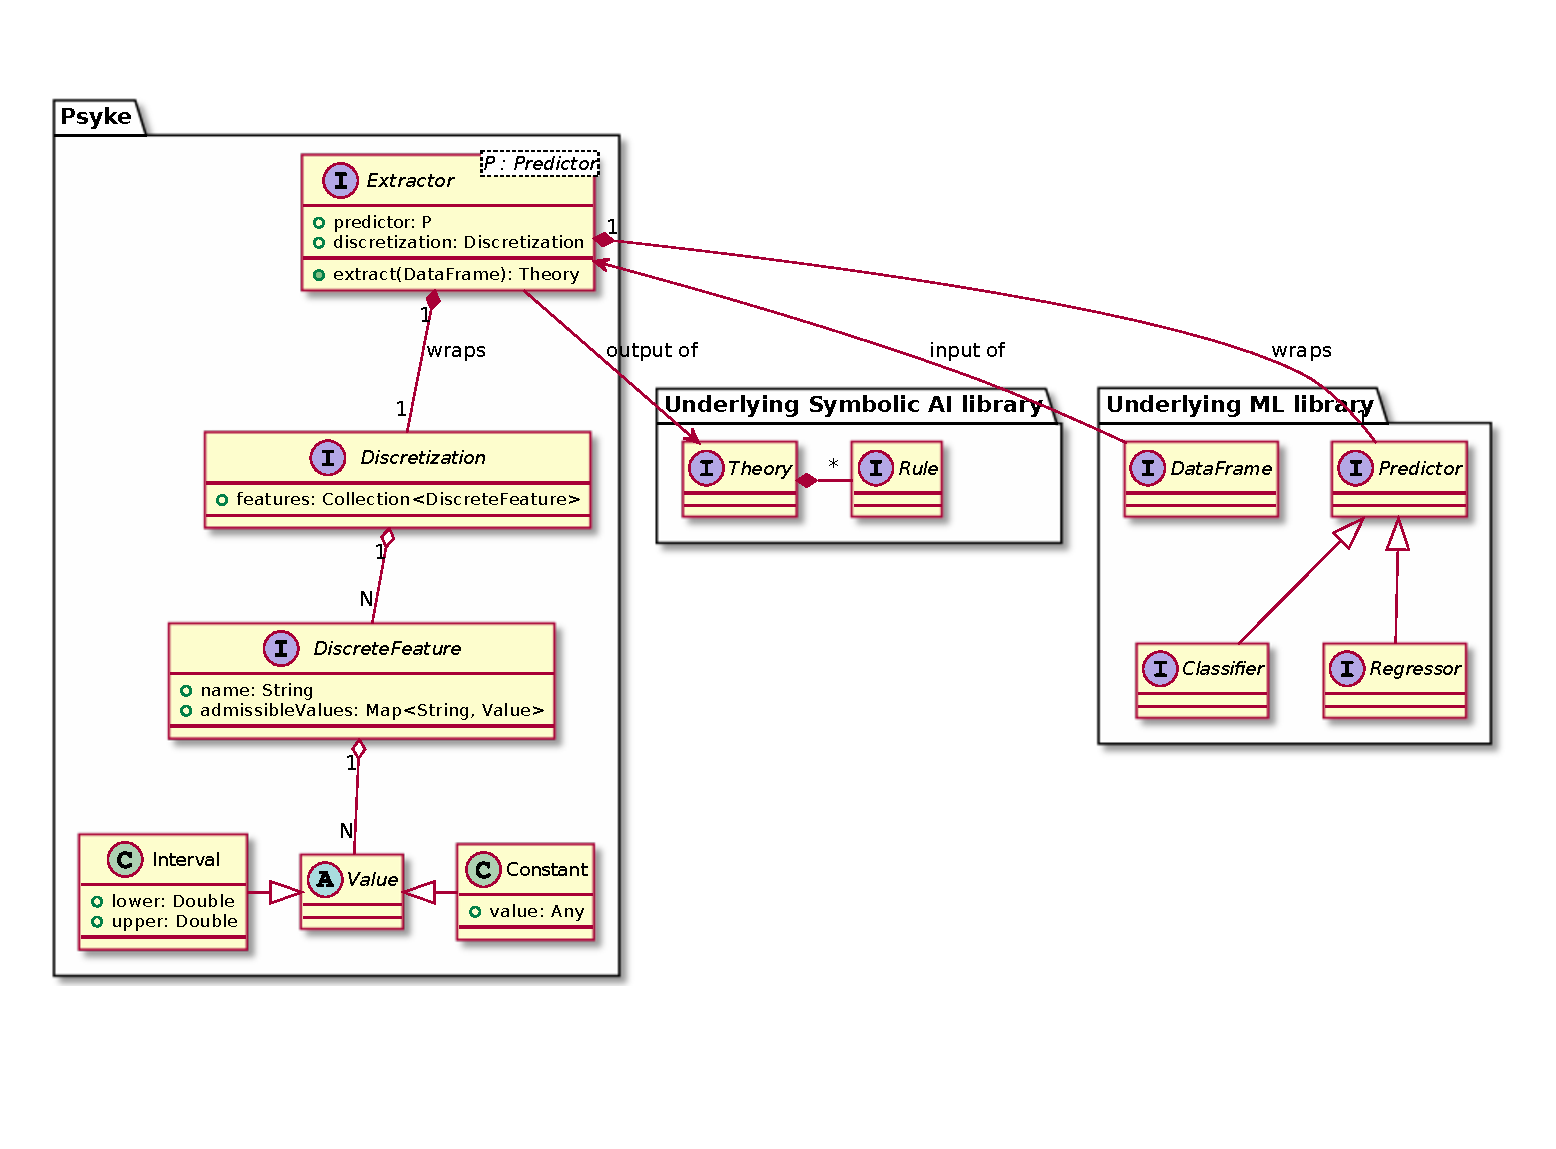
\includegraphics[width=\linewidth]{figures/extractor-api.pdf}
    \caption{\psyke{}'s \kt{Extractor} interface}
    \label{fig:extractor-api}
\end{figure}

As depicted in \cref{fig:extractor-api}, a pivotal role in the design of \psyke{} is played by the \kt{Extractor} interface, defining the general contract of any knowledge-extraction procedure.
%
Technically, each \kt{Extractor} encapsulates a single ML \kt{Predictor} and a particular \kt{Discretization} strategy for the data it operates upon.
%
Under such conditions, an extractor is capable of extracting a \kt{Theory} of logic \kt{Rule}s out of a \kt{DataFrame}, containing the examples the \kt{Predictor} has been trained upon.

A relevant aspect of \psyke{} design -- and a prerequisite for its understanding --, is that it avoids re-inventing the AI wheel.
%
Thus, \psyke{} assumes that some underlying libraries are available on the runtime adopted for implementation, from which AI facilities can be inherited.
%
These include:
%
\begin{inlinelist}
    \item a ML library, exposing \emph{ad-hoc} types aimed at representing data sets, data schemas, or predictors, and
    \item a symbolic AI library, exposing \emph{ad-hoc} types for representing and manipulating logic theories, clauses, and rules.
\end{inlinelist}
%
From these libraries, \psyke{} borrows high-level abstractions, required for its operation, which would be prohibitive to re-design or re-implement from scratch.
%
These include, for instance, the following types:
%
\begin{description}
    \item[\kt{DataFrame}] --- a container of tabular data, where rows commonly denote instances, and columns denote their features, while bulk operations are available to manipulate the table as a whole, as well as any row/column of its;
    \item[\kt{Predictor<R>}] --- a computational entity which can be trained (a.k.a.\ fitted) against a \kt{DataFrame} and used to draw predictions of type \kt{R};
    \item[\kt{Classifier<R>}] --- a particular case of predictor where \kt{R} represents a type having a finite amount of admissible values;
    \item[\kt{Regressor<R>}] --- a particular case of predictor where \kt{R} represents a type having a potentially infinite (possibly continuous) amount of admissible values;
    \item[\kt{Rule}] --- a semantic, intelligible representation of the function mapping \kt{Predictor}'s inputs into the corresponding outputs, for a particular portion of the input space;
    \item[\kt{Theory}] --- an ordered collection of rules.
\end{description}
%
For example, \psyke{} may borrow ML-related abstractions -- such as \kt{DataFrame}, \kt{Predictor}, or \kt{Classifier} -- from either \smile{} or \scikit{}, depending on the particular runtime of choice (among JVM or Python), or any library serving the same purpose and exposing analogous abstractions.
%
Similarly, it may borrow high-level symbolic-AI-related abstractions -- such as \kt{Theory} or \kt{Rule} -- from \twopkt{} \cite{cco-softwarex-2021-2pkt} which supports both the JVM\footnote{\url{https://github.com/tuProlog/2p-kt}} and Python\footnote{\url{https://github.com/tuProlog/2ppy}} runtimes---and of course any functionally-equivalent library could be used as well.

Upon such premises, \psyke{} constructs a notion of \kt{Extractor}---i.e., any method capable of extracting logic \kt{Rule}s out of some trained \kt{Predictor}.
%
In our design, \psyke{} extractors are bound to the particular black-box \kt{Predictor} they aim to extract rules from, as well as a \kt{Discretization} strategy for its input space.
%
These fields are provided upon instantiation, and never altered since then.
%
\kt{Extractor}s also expose:
%
\begin{inlinelist}
    \item a method for extracting an explainable \kt{Theory} from the \kt{Predictor} -- namely, \kt{extract} -- and
    \item a method to draw predictions by using the extracted rules---namely, \kt{predict}.
\end{inlinelist}
%
Of course, prediction implies extraction---meaning that each attempt to use the extracted rules to draw explainable predictions shall trigger extraction first.
%
Both extraction and prediction rely on a \kt{DataFrame} which must be provided by the user upon invocation.
%
It should contain the data the predictor has been trained upon -- or some structurally analogous data --, in order to let the extraction algorithm determine the structure of the extracted rules.

Notice that \kt{Predictor}s are parametric types.
%
There, the meta-parameter \kt{R} represents the type of predictions the predictor may produce---unknown at design time.
%
%In practice, depending on the particular data and predictors of choice, the extraction and prediction procedures may vary significantly on this aspect.
The rules possibly extracted by such predictors -- as well as the predictions drawn from them -- may vary significantly depending on the particular data and predictors of choice.
%
For instance, when rules must be extracted from mono-dimensional regressors, \kt{R} may be the type of floating point numbers, whereas for multi-class classifiers, \kt{R} may consist of the set of types (like integer, string, etc.).
% \fsnote{set of classes non mi suona tanto. Cioè, set di stringhe, set di interi, ok, ma set di classi non mi suona come un tipo}
%
Of course, the rules possibly extracted by such predictors greatly differ, depending on the nature of \kt{R}.
%\fsnote{questa mi pare un po' una ripetizione della frase che inizia con in practice. Tu vuoi segnalare che le procedure variano e variano anche le regole, in base a R. Propongo una frase unica che le comprende entrambe}
%
However, the proposed API makes it possible to switch between different extraction algorithms and predictors requiring no changes in the architecture of \psyke{}, but only minor adjustments in the user code.

\subsection{Discretisation}

A large number of the knowledge-extraction procedures -- in the same way as many ML algorithms -- require either a discrete or binary input space---i.e.\ all input features must be either categorical or one-hot encoded, respectively.
%
For instance, \real{} and \trepan{} require exclusively one-hot encoded data, whereas \iter{} and \gridex{} require continuous data.
%
\cart{} can accept both continuous and one-hot encoded features, but not categorical ones.
%
Unfortunately, most real-world applications are described by real-valued variables and measurements, thus making the application of such algorithms impractical.
%
The general way to overcome this limitation is to rely on some discretisation/binarisation method among the many available in the literature---e.g., \cite{DoughertyKS95,YangWW10,Kerber92,HoS97,Boulle04,KurganC04,Cano2016}.

Briefly speaking, discretisation is the process of transforming a datum from some continuous space $I \subseteq \mathbb{R}$ into a discrete space $\{ I_1, \ldots, I_n \}$ such that $\forall i,j  = 1, \ldots, n$:
%
% \begin{itemize}
% \item
$I_i \subset I$
$\wedge$ % \item
$I \equiv \bigcup_i I_i$
$\wedge$ % \item
$i \neq j \Leftrightarrow I_i \cap I_j = \varnothing $
$\wedge$ % \item
$i < j \Leftrightarrow \forall x \in I_i, \forall y \in I_j : x < y $.
% \end{itemize}
%
Similarly, binarisation (a.k.a. one-hot encoding) is the process of transforming a datum from some discrete space $X = \{x_1, \ldots, x_n \}$ into a binary space $B = \{ b_1, \ldots, b_{n} \}$ where for each $i  = 1, \ldots, n$: $b_i$ is $1$ if the datum is equal to $x_i$, $0$ otherwise.
%
Of course, these methods imply a considerable increase in the dimensionality of a data set---e.g., one-hot encoding makes categorical attributes with 4 distinct values be converted into 4 different boolean features.
%
This is far from being an issue: in some cases, it is possible to achieve even better classification performances by using discretised attributes rather than continuous, as demonstrated in \cite{ElhilbawiE021}.

\psyke{} provides different procedures to manipulate input features:
%
\begin{inlinelist}
    \item a discretisation for continuous features, mapping real intervals into categorical features, and
    \item a one-hot encoding for categorical features, mapping exact values to boolean features.
\end{inlinelist}
%
Notably, \psyke{} traces the input feature transformations by creating a data structure that associates the initial name of the attribute and the newly created features with the corresponding constraints.
%
An example of \psyke{} binarisation and corresponding output data structure is reported in \cref{fig:discretisation}.
%
This example considers the \emph{petal length} attribute of the Iris data set and adopts the default supervised discretisation method available in our framework.
%
The initial continuous feature values are labelled in \cref{fig:discretisation} with a), and graphically represented in the b1) plot.
%
\psyke{} discretisation algorithm consists in calculating the mean attribute value and the corresponding standard deviation \emph{for each data set class}.
%
An interval is then initialised for each class, with lower and upper bounds equal to the mean value---cf. plot b2).
%
Each interval is iteratively expanded until convergence---i.e., when the whole feature space is covered without overlapping intervals.
%
To achieve this, during every iteration all the intervals are symmetrically expanded of a value equal to the corresponding standard deviation -- in each direction, as in plot b3) --, in order to create intervals with adaptive size.
%
An expansion is inhibited when
%
\begin{inlinelist}
    \item the lower (upper) bound of an interval exceeds the minimum (maximum) value of the feature space, or
    \item two adjacent intervals are overlapping.
\end{inlinelist}
%
In the first case, the feature minimum (maximum) value is taken as the final interval lower (upper) bound.
%
In the second case, the overlapping intervals are only expanded up to the mean value between their respective boundaries.
%
When all intervals have been calculated -- cf. plot b4) -- the continuous attribute values are converted accordingly into categorical values.
%
The discretised output values are labelled in the example with c).
%
In this step \psyke{} also produces a data structure for keeping the discretisation details, to be able to produce more compact rules during the extraction procedures.
%
The last step -- labelled with d) -- is the one-hot encoding of the discrete values into arrays of binary data---i.e., the unique format accepted by several extraction procedures, such as \real{} and \trepan{}.

\begin{figure}
    \centering
    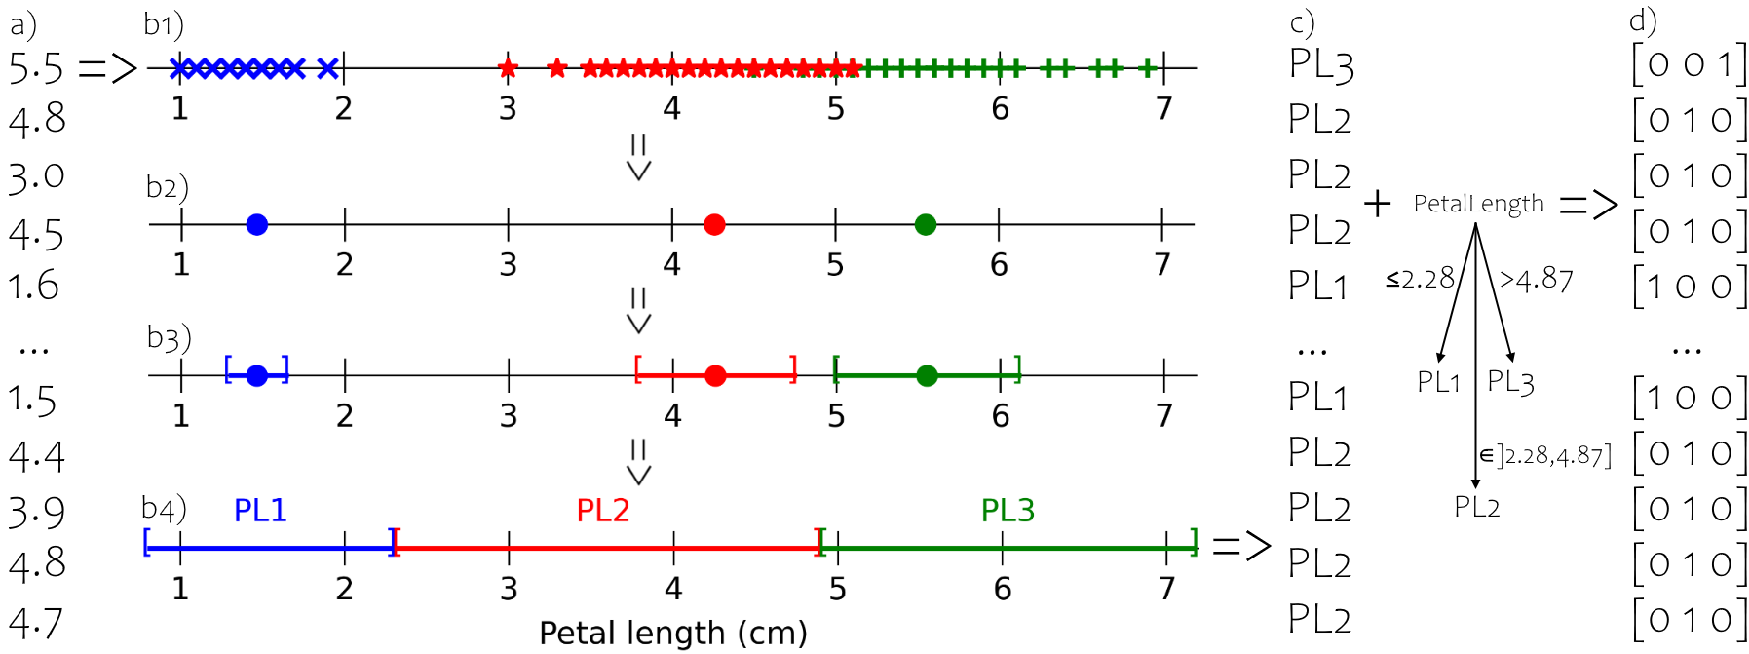
\includegraphics[width=\linewidth]{figures/disc.pdf}
    \caption{\psyke{} discretisation and binarisation procedure}
    \label{fig:discretisation}
\end{figure}

\subsection{Output rules}

%\subsubsection{Classification}

\psyke{} extractors output knowledge in the form of logic theories -- i.e., lists of Horn clauses --, notably in Prolog syntax.
%
We choose the Prolog syntax to make them simultaneously interpretable by both humans and machines.
%
More precisely, \psyke{} output theories are structured as lists of Prolog rules or facts.
%
Rule heads are $(n+1)$-ary predicates, where $n$ is the number of input features in the data set.
%
These predicates carry $n$ variables -- i.e., one for each input feature -- and either a constant or a list -- i.e., the output value(s) -- as argument.
%
Predicate names recall the classification/regression under study.
%
Rule bodies can be empty -- if rules are \emph{facts} -- or conjunctions of literals where each literal is a predicate expressing inequality, equality, or interval inclusion between attribute actual values and fixed constants calculated through the extraction process.

Accordingly, a rule-extraction procedure targeting a mono-dimensional classification $task$ on a data set having $n$ input features and $m$ relevant output values, shall output theories of the following form:
%
\begin{equation*}
    %    \scriptsize
    \begin{array}{rcl}
        \logicrule{\meta{task}(\var{X}_1, \ldots, \var{X}_n, \const{y}_1)}{p_{1,1}(\bar{\var{X}}),\ \ldots,\ p_{n,1}(\bar{\var{X}})}.
        \\
        \logicrule{\meta{task}(\var{X}_1, \ldots, \var{X}_n, \const{y}_2)}{p_{1,2}(\bar{\var{X}}),\ \ldots,\ p_{n,2}(\bar{\var{X}})}.
        \\
        & \vdots
        \\
        \logicrule{\meta{task}(\var{X}_1, \ldots, \var{X}_n, \const{y}_m)}{p_{1,m}(\bar{\var{X}}),\ \ldots,\ p_{n,m}(\bar{\var{X}})}.
    \end{array}
\end{equation*}
%
where
%
\begin{inlinelist}
    \item $\mathit{task}$ is the $(n+1)$-ary relation representing the classification or regression task at hand,
    \item each $\var{X}_i$ is a logic variable named after the $i^{th}$ input attribute of the currently available data set,
    \item $\bar{\var{X}}$ is the $n$-nuple $\var{X}_1, \ldots, \var{X}_n$, and
    \item each $p_{i,j}$ is either a $n$-ary predicate expressing some constraint about one, two or more variables, or the \pl{true} literal---which can be omitted.
\end{inlinelist}

Similarly, a rule-extraction procedure targeting a mono-dimensional regression $task$ shall output theories of the following form:
%
\begin{equation*}
    \begin{array}{rcl}
        \logicrule{\meta{task}(\var{X}_1, \ldots, \var{X}_n, \var{Y})}{p_{1,1}(\bar{\var{X}}),\ \ldots,\ p_{n,1}(\bar{\var{X}}), \var{Y}\ \var{is}\ f_1(\bar{\var{X}})}.
        \\
        \logicrule{\meta{task}(\var{X}_1, \ldots, \var{X}_n, \var{Y})}{p_{1,2}(\bar{\var{X}}),\ \ldots,\ p_{n,2}(\bar{\var{X}}), \var{Y}\ \var{is}\ f_2(\bar{\var{X}})}.
        \\
        & \vdots
        \\
        \logicrule{\meta{task}(\var{X}_1, \ldots, \var{X}_n, \var{Y})}{p_{1,m}(\bar{\var{X}}),\ \ldots,\ p_{n,m}(\bar{\var{X}}), \var{Y}\ \var{is}\ f_m(\bar{\var{X}})}.
    \end{array}
\end{equation*}
%
where $\meta{task}$, $\var{X}_i$, $\bar{\var{X}}$, and $p_{i,j}$ have the same meaning than the classification case, whereas
%
\begin{inlinelist}
    \item $f_j$ is an $n$-ary function computing the output value for the regression task in the particular portion of the input space handled by the $j^{th}$ rule, and
    \item $\var{is/2}$ is the well-known Prolog predicate aimed at evaluating functions.
\end{inlinelist}

Without lack of generality, the aforementioned rule forms assume the case under study to involve \emph{mono-dimensional} classification/regression tasks.
%
In fact, multi-dimensional cases can be tackled by allowing lists of constants -- e.g. $\var{[}\const{y}^{(1)}, \const{y}^{(2)}, \ldots \var{]}$ -- in the heads of classifications rules; or lists of variables -- e.g. $\var{[Y}^{(1)}, \var{Y}^{(2)}, \ldots \var{]}$ -- in the head of regression rules, as well as multiple variable assignments in their bodies---e.g. $\var{Y}^{(1)}\ \var{is}\ f_j^{(1)}(\bar{\var{X}}), \var{Y}^{(2)}\ \var{is}\ f_j^{(2)}(\bar{\var{X}}), \ldots$

The rationale behind our proposed way of structuring rules is straightforward: the $j^{th}$ rule selects a portion of the input space via a number of constraints $p_{1,m}(\bar{\var{X}}),\ \ldots,\ \allowbreak p_{n,m}(\bar{\var{X}})$ -- which may be less than $n$ in practice --, and then dictates the most adequate prediction for that portion.
%
In classification tasks, the prediction is constant for the whole portion, whereas in regression tasks it is computed via a function $f_j(\bar{\var{X}})$.
%
This function may itself output a constant in simpler cases, or a local approximation of the predictor's behaviour in the corresponding portion of the input space---e.g. a linear approximator.
%
Notice that, in classification tasks, the total amount of rules ($m$) may still be greater than the total amount of classes ($k$), as there may be more than one rule for the same class. % in the general case.
%
In the general case, $m$ is bound to the number of portions of the input space detected by the extraction algorithm of choice.

Currently, the supported sorts of predicates in rules bodies -- i.e., the admissible shapes for each $p_{i,j}$ -- are as follows:
%
\begin{description}
    \item[equality] involving a single variable and a constant---e.g. $\var{X} = c$, where $c$ is a constant of any sort (possibly, a number)
    \footnote{The same result could be attained by allowing constants in rules heads}
    %
    \item[inequalities] involving a single variable and a constant---e.g. $\var{X} \gtrless c$
    \item[interval inclusion] involving a single variable and two constants---e.g. $\var{X} \texttt{ in [}l, u\texttt{]}$, where $l,u \in \mathbb{R}$ and $l < u$
    \item[interval exclusion] like the above, but negated---e.g. $\var{X} \texttt{ not\_in [}l, u\texttt{]}$
    \item[\mofn{}] involving $N$ variables---e.g. $\texttt{at\_least}(M, \allowbreak \texttt{[} \var{X}_1, \ldots, \var{X}_N \texttt{]})$, where $M, N \in \mathbb{N}_{\geq 0}$
\end{description}
%
%\gcnote{Nel caso della refressione abbiamo anche il parametro d'uscita da gestire. In tal caso potremmo voler assegnare un'intera funzione ad esso. Io descriverei la cosa esplicitamente.}
This holds for both classification and regression tasks.

Despite many other forms can be adopted for the output theories, we argue the proposed one is a good trade-off between human and machine interpretability.
%
In fact, rules of this form are well-formed logic programs, which may be executed by a logic reasoner---such as a Prolog interpreter.
%
Furthermore, the proposed form is open to many sorts of post-processing.
%
For instance, recurrent conjunctions of predicates in rules bodies may be factorised into their own general-purpose rules.
%
Similarly, redundant or cumbersome sub-expressions may be simplified.
%
%\gcnote{Potremmo fare esempi di semplificazioni successive per allungare il brodo}

However, the proposed form is far from perfection: we plan to explore alternative directions in the future.
%
Noticeably, using Prolog syntax does not impose exploiting also its semantics---i.e., different interpreters can be exploited over such Prolog rules.
%
For instance, on the one side, by exploiting a Prolog interpreter, rules are interpreted as functional (one-way)---meaning that it is possible to compute a prediction given an assignment of all input variables, but it is not possible to generate a correct assignment of those input variables given the expected prediction alone.
%
On the other side, a Constraint Logic Programming solver \cite{GavanelliR10,JaffarM94} may interpret the same rules as constraints, and compute coherent assignments for any subset of both input and output variables---providing rules with a relational (two-ways, generative) semantics.

\section{Case Study}\label{sec:experiments}

In this section the effectiveness and versatility of \psyke{} are tested by exploiting it in different scenarios---i.e.\ the Iris data set\footnote{\vurl{https://archive.ics.uci.edu/ml/datasets/iris}} as classification task and the Combined Cycle Power Plant\footnote{\vurl{https://archive.ics.uci.edu/ml/datasets/combined+cycle+power+plant}} (CCPP) data set as a regression case study.
%
Examples of output rules extracted with \psyke{} algorithms are reported, along with a brief discussion on several possible future improvements for the rule final presentation (see \cref{ssec:discussion}).
%
\Cref{fig:datasets} reports the sample distribution of the Iris and CCPP data sets, with respect to their two most relevant respective features---i.e., petal width and length for the Iris data set (\cref{fig:iris}) and ambient temperature and exhaust vacuum for the CCPP data set (\cref{fig:ccpp}).
%
% !TeX root = ../phd-thesis.tex

\begin{figure*}
	\centering
	\subfloat[Iris]{
		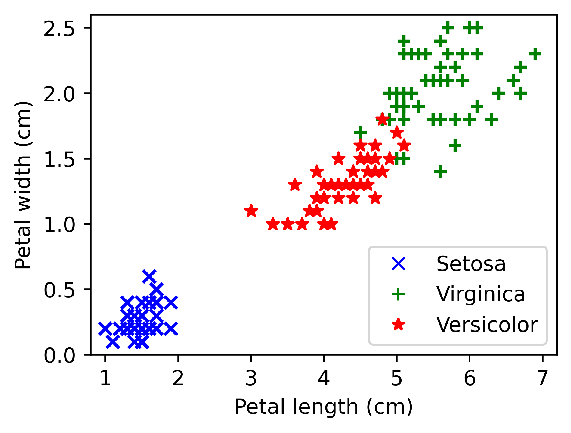
\includegraphics[width=0.45\linewidth]{figures/CLA/iris-samples.pdf}
		\label{fig:iris}
	} %}
	\subfloat[CCPP]{
		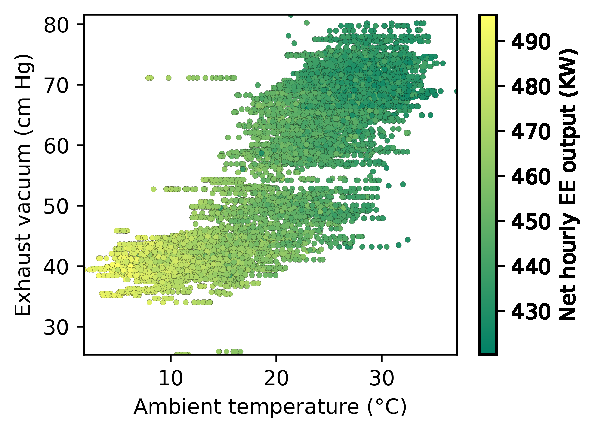
\includegraphics[width=0.47\linewidth]{figures/REG/ccpp-samples.pdf}
		\label{fig:ccpp}
	}
	\caption[Sample distribution of the Iris and CCPP data sets]{Sample distribution of the Iris and CCPP data sets. Only the 2 most relevant features are reported.}
	\label{fig:datasets}
\end{figure*}

\subsection{Classification: the Iris data set}
%
In this case study we exploit \psyke{} to extract Prolog rules on a number of classifiers trained on the well-known Iris data set.
%
Notably, the Iris data set contains 150 rows describing as many individuals of the Iris flower.
%
For each exemplary, 4 continuous input features -- petal and sepal width and length -- are recorded, other than a categorical class label---i.e., which particular sort of Iris plant the exemplary has been classified as.
%
There are three particular sub-sorts of Iris in this data set -- namely, Setosa, Virginica, and Versicolor --, and the 150 examples are evenly distributed among them---i.e., there are 50 instances for each class.

The experimental setting is as follows.
%
First, we train 3 different sorts of classifiers on the Iris data set---namely, a k-nearest-neighbors (kNN), a multi-layer perceptron (MLP), and a decision tree (DT).
%
Then we let \psyke{} extract logic rules out of these classifiers using as many extraction procedures.
%
In particular, we rely on \real{}, \trepan{}, and \cart{}.
%
A portion (50\%) of the original data set -- namely, the test set -- is put aside \emph{before} training to later enable the evaluation of the extracted rule predictive performance.

Accordingly, within the scope of this experiment, we rely on \emph{accuracy} as the preferred metric for both predictive performance and fidelity---where the former measures how good a classifier or the corresponding extracted rules are in classifying Iris instances in absolute terms, while the latter measures the adherence of the extractor output rules w.r.t.\ the original classifier.

\subsubsection{The experiment}

Let us assume the Iris data set can be loaded from a CSV file via a script using one of the third-party libraries exploited by \psyke{}---i.e., \scikit{} or \smile{} for Python or JVM users, respectively.
%
The Iris data set only contains continuous features.
%
Therefore, \cart{} is the only algorithm that can be \emph{directly} applied to it, whereas \real{} and \trepan{} can only operate on binary data.
%
Accordingly, \psyke{} provides a simple two-step procedure to binarise the data, involving both discretisation and one-hot encoding: a data set can be discretised, one-hot encoded, and split into training and test set via a couple of instructions, providing the percentage of samples to be taken apart from the whole data set to attain the test set.
%
As the next step, we train 4 different classifiers on the training set---namely a kNN, a MLP, and two DT---one with the original, continuous data set, and one with its binarised version\footnotemark.
\footnotetext{Code of experiments is available at \url{https://github.com/psykei/psyke-jvm} and \url{https://github.com/psykei/psyke-python}}
%\fsnote{Aggiungere rif. a scikit oppure togliere rif \smile{} nella footnote}
%
Finally, in the following paragraphs, we show how rules can actually be extracted and what their ultimate shape actually is.

\subsubsection{\real{}}\label{sssec:real}

\psyke{}'s \real{} algorithm can be applied to any BB classifier accepting binary input features---e.g., among the aforementioned models only the DT trained upon the continuous data set is not suitable to apply this extraction technique.
%
The extracted theory is dependent on the training set; different training instances can produce different rules, resulting in slight variations also in the output theory complexity---intended as the number of clauses and terms.
%
An example of \real{} applied to a MLP is reported in the following:
%
\prologimport[nolol]{listings/iris-real.pl}

The theory produces an input space partitioning as reported in \cref{fig:real-mlp}.
%
It is worthwhile to notice that -- especially with more complex data sets -- the partitioning could be non-exhaustive---i.e., the logic rules could be unable to classify some samples.

\subsubsection{\trepan{}}

\psyke{} provides a \trepan{} algorithm applicable under the same constraint described above for \real{} and also its output rules can vary with different training sets.
%
Differently from \real{}, \trepan{} accepts as input 3 optional parameters
%
stating the minimum number of samples to consider for performing further splits (\kt{minExamples}, default: 0), the maximum depth of the produced tree (\kt{maxDepth}, default: 0, i.e.\ no constraints), and the criterion to adopt for the best split selection (\kt{splitLogic}).
%
At the moment \psyke{} can only adopt a default \kt{splitLogic} to assign a binary split  to each \trepan{} node.
%
The method is based on the selection of the most discriminating feature at each split, i.e., the feature having higher probability to produce a tree leaf containing all the samples belonging to a specific class without containing samples of other classes.
%
We plan to implement in the future other methods for \emph{if-then} splits as well as for \mofn splits.

An example of output theory obtained by applying \trepan{} to a 5-NN is reported in the following:
%
\prologimport[nolol]{listings/iris-trepan.pl}
%
This theory produces an input space partitioning as reported in \cref{fig:trepan-knn}.
%
In this case, the partitioning is always exhaustive.

\subsubsection{\cart{}}\label{sssec:cartClass}

\cart{} is the third algorithm included in \psyke{} to tackle classification tasks.
%
It is directly applicable to DT classifiers and in this case it does not require any extra parameter, since the extraction only relies on the tree structure of the decision tree---that is, all the parameters have to be tuned during the DT creation and training.
%
Otherwise, \cart{} can be applied to other kinds of classifiers, but this implies the creation of an intermediate tree structure and thus to have greater control on the output quality it is advisable to impose a maximum value for the tree depth or the number of leaves.

\psyke{}'s \cart{} algorithm can operate with both one-hot encoded and continuous input features.
%
In the same way as many other algorithms, \cart{} is able to achieve comparable or even better results when relying on a good discretisation/one-hot encoding technique.
%
In the following an example of theory obtained with \cart{} applied to the DT trained with the continuous Iris data set is reported:
%
\prologimport[nolol]{listings/iris-cart.pl}
%
\Cref{fig:cart-dt-cont} reports the corresponding input space partitioning.
%
The output rules are always exhaustive.
%
The same data set, but previously one-hot encoded, leads to the following theory and to the partitioning reported in \cref{fig:cart-dt-cla}:
%
\prologimport[nolol]{listings/iris-cart-1hot.pl}

\subsubsection{Results}\label{sssec:resultsClass}

% !TeX root = ../phd-thesis.tex
\begin{figure}
	\centering
	\begin{tabular}{c|ccc}
		Predictor & \real{} & \trepan{} & \cart{} \\
		\hline
        \hline
		\subfloat[5-NN.]{
			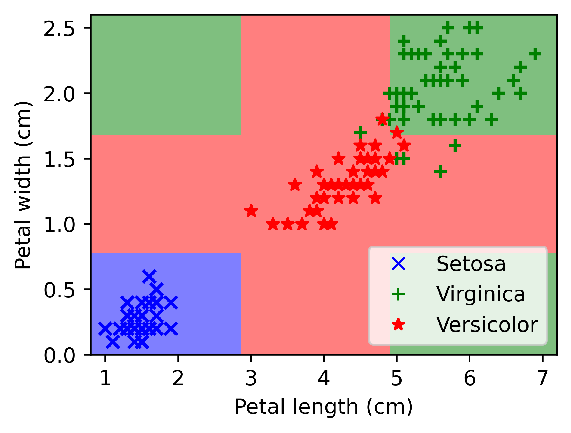
\includegraphics[width=0.20\linewidth]{figures/CLA/bb-knn.pdf}
			\label{fig:bb-knn}
		} &
		\subfloat[]{
			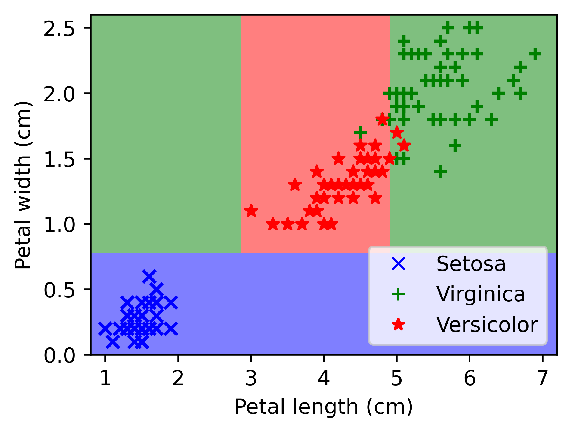
\includegraphics[width=0.20\linewidth]{figures/CLA/real-knn.pdf}
			\label{fig:real-knn}
		} &
		\subfloat[]{
			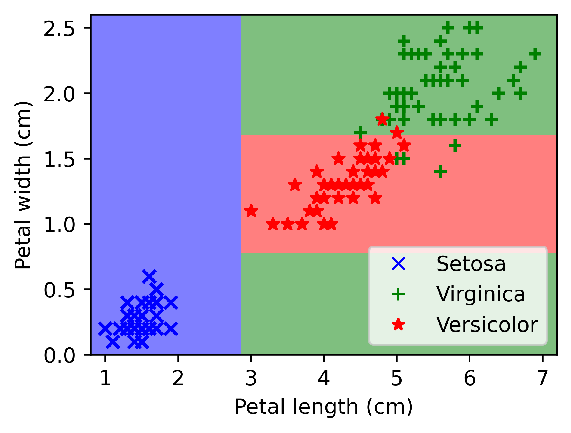
\includegraphics[width=0.20\linewidth]{figures/CLA/trepan-knn.pdf}
			\label{fig:trepan-knn}
		} &
		\subfloat[]{
			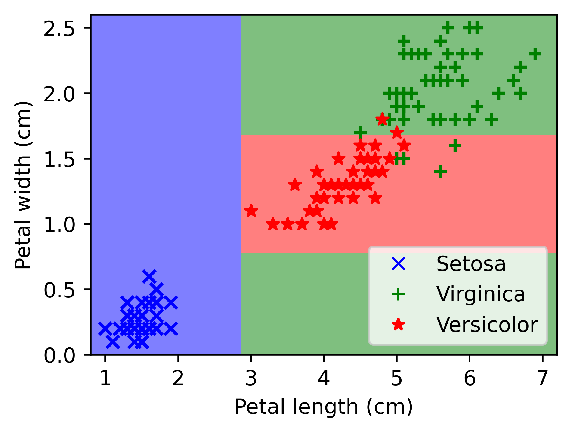
\includegraphics[width=0.20\linewidth]{figures/CLA/cart-knn.pdf}
			\label{fig:cart-knn}
		}
		\\
		\subfloat[MPL.]{
			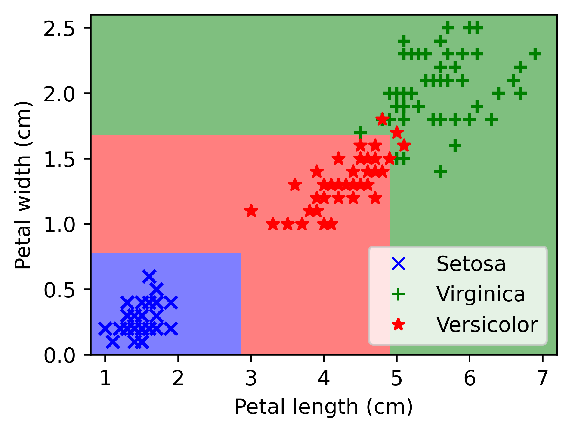
\includegraphics[width=0.20\linewidth]{figures/CLA/bb-mlp.pdf}
			\label{fig:bb-mlp-cla}
		} &
		\subfloat[]{
			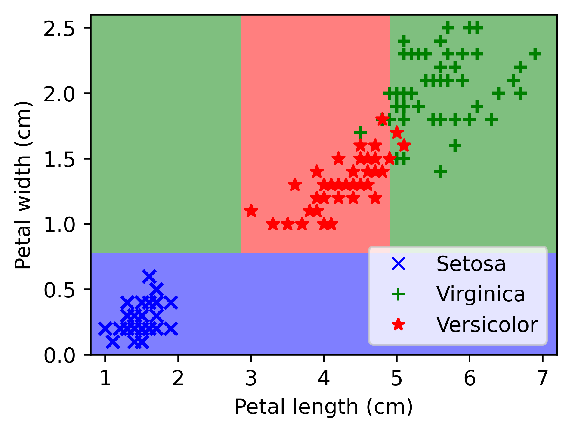
\includegraphics[width=0.20\linewidth]{figures/CLA/real-mlp.pdf}
			\label{fig:real-mlp}
		} &
		\subfloat[]{
			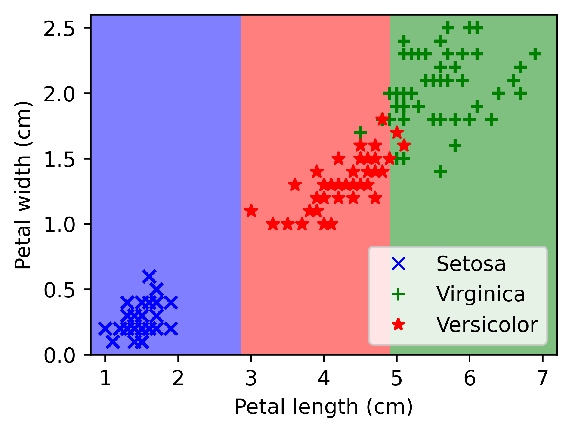
\includegraphics[width=0.20\linewidth]{figures/CLA/trepan-mlp.pdf}
			\label{fig:trepan-mlp}
		} &
		\subfloat[]{
			\includegraphics[width=0.20\linewidth]{figures/CLA/cart-mlp.pdf}
			\label{fig:cart-mlp-cla}
		}
		\\
		\subfloat[DT (binarised features).]{
			\includegraphics[width=0.20\linewidth]{figures/CLA/bb-dt.pdf}
			\label{fig:bb-dt-cla}
		} &
		\subfloat[]{
			\includegraphics[width=0.20\linewidth]{figures/CLA/real-dt.pdf}
			\label{fig:real-dt}
		} &
		\subfloat[]{
			\includegraphics[width=0.20\linewidth]{figures/CLA/trepan-dt.pdf}
			\label{fig:trepan-dt}
		} &
		\subfloat[]{
			\includegraphics[width=0.21\linewidth]{figures/CLA/cart-dt.pdf}
			\label{fig:cart-dt-cla}
		}
		\\
		\subfloat[DT (continuous features).]{
			\includegraphics[width=0.21\linewidth]{figures/CLA/bb-dt-cont.pdf}
			\label{fig:bb-dt-cont}
		} & & &
		\subfloat[]{
			\includegraphics[width=0.21\linewidth]{figures/CLA/cart-dt-cont.pdf}
			\label{fig:cart-dt-cont}
		} \\
	\end{tabular}
	\caption[Comparison between Iris data set input space partitionings performed by the algorithms implemented in \psyke{}]{Comparison between Iris data set input space partitionings performed by the algorithms implemented in \psyke{}. Only the two most relevant features are reported---i.e., petal width and length. Missing subplots are due to the impossibility to apply \real{} and \trepan{} to BB classifiers trained with continuous input features}
	\label{fig:irisAll}
\end{figure}

% !TeX root = ../phd-thesis.tex

\begin{table}
	\caption{Comparison between accuracy and fidelity measurements with different combinations of extraction algorithms and underlying models applied to the Iris dataset}
	\label{tab:comparison}
	\begin{adjustbox}{width=\linewidth}
        \begin{tabular}{ll@{\hskip 0.8in}lll}
            \hline
            \multicolumn{2}{l}{\textbf{Predictor}} &
            \multicolumn{3}{@{}l}{\textbf{Extractor}}\\
            \textbf{Type} & \textbf{Accuracy} & \textbf{Algorithm} & \textbf{Fidelity} & \textbf{Accuracy} \\
            \hline\hline
            5-NN & 0.94 & \real{} & 0.98 & 0.95 \\
            & & \trepan{} & 0.95 & 0.95 \\
            & & \cart{} & 0.95 & 0.95 \\
            \hline
            MLP & 0.98 & \real{} & 0.98 & 0.95 \\
            & & \trepan{} & 0.98 & 0.92 \\
            & & \cart{} & 0.98 & 0.92 \\
            \hline
            DT (binarised features) & 0.98 & \real{} & 0.98 & 0.97 \\
            & & \trepan{} & 0.98 & 0.92 \\
            & & \cart{} & 1.00 & 0.98 \\
            \hline
            DT (continuous features) & 0.95 & \cart{} & 1.00 & 0.95 \\
            \hline
        \end{tabular}
    \end{adjustbox}
\end{table}


In the following we report the results of \real{}, \trepan{}, and \cart{} applied to the Iris data set.
%
All the results are resumed in \cref{fig:irisAll} and \cref{tab:comparison}.
%
Column ``Predictor'' represents the ML step of the process.
%
Accordingly, \cref{fig:bb-knn,fig:bb-mlp-cla,fig:bb-dt-cla,fig:bb-dt-cont} represent the decision boundaries of a 5-NN predictor, a MLP and 2 decision trees, respectively.
%
The first DT is trained with the binarised version of the Iris data set; the other with the original continuous values.
%
Finally, column ``Extractor'' represents the output of \psyke{}.
%
In particular, different extraction procedures -- namely, \real{}, \trepan{}, and \cart{} -- are applied to the 4 BB predictors.
%
\real{} and \trepan{} are not applied to the DT trained with the continuous data set because these extraction procedures cannot handle real-valued input features.

It is worth noticing that
%
\begin{inlinelist}
    \item \cart{} always produces a partitioning equivalent to those of the underlying BB model when the model is a DT, because of its design, and
    \item each extractor's output partitioning may be different from other extractors' ones -- for instance a procedure may only use the petal width attribute, another procedure may only use the petal length attribute, while other procedures may use both input features, combined in several ways --, but all solutions share a similar predictive performance.
\end{inlinelist}

A numerical assessment of the aforementioned predictors and extractors is reported in \cref{tab:comparison}.
%
Values are averaged upon 25 executions, each one with different random train/test splits, but same test set percentage and same parameters for predictors and extractors.
%
The table reports the underlying predictor accuracy as well as the fidelity and accuracy of the extraction procedure.
%
We plan to enhance comparisons between different extractors through fidelity assessments carried out by measuring the decision boundary overlapping regions.

\Cref{tab:comparison} shows how the \cart{} extractor always has a fidelity of 1.0 when applied to a DT, since it only inspects the underlying decision tree nodes to build its output rules without any information loss.
%
This implies that \psyke{}'s \cart{} extractor is an equivalent (yet explainable) alternative to DT models, as it produces the same output predictions.
%
As for the other extractors, both \real{} and \trepan{} are able to achieve good results in terms of fidelity and accuracy -- always above 0.9 in our experiments -- in some cases even with a better performance w.r.t.\ the original model.

\subsection[Regression: the CCPP dataset]{Regression: the Combined Cycle Power Plant dataset}

In our second case study, \psyke{} is exploited to extract Prolog rules out of different BB regressors trained upon the CCPP data set.
%
The data set contains 9568 instances, each one composed of 4 real-valued input attributes -- i.e., ambient temperature and pressure, relative humidity and exhaust vacuum -- and one real-valued output feature---i.e., the net hourly electrical energy output of the plant.

For this experiment, 3 different regressors are trained on the CCPP data set: a linear regressor (LR), a MLP and a DT.
%
Then, as for the classification case, \psyke{} is exploited to extract logic rules out of these BB models by using all the applicable supported procedures---namely, \iter{}, \gridex{} and \cart{}, each one applied to all the aforementioned ML predictors.
%
The data set portion isolated as test set for this experiment is equal to 20\%.
%
To assess the predictive performance of BB predictors and extractors as well as the fidelity of extractors w.r.t.\ the underlying models mean absolute error (MAE) and R$^2$ score are adopted.

\subsubsection{The experiment}

The CCPP data set can be loaded from a CSV file.
%
Since it only contains continuous attributes, and since this sort of feature is the only one accepted by \psyke{} extractors for regression tasks, no discretisation or binarisation steps are required.
%
However, since the input features have very different ranges of values, a normalisation or standardisation pre-processing is suggested to have more robust BB training phases.
%
For this experiment, a standardisation has been applied to the input features.
%
The operation must be revertible, because extraction techniques applied to BB models trained with standardised (or normalised) data will produce rules containing standardised (or normalised) values.
%
Thus, to obtain human-understandable rules a further inverse transformation is required.

In the following paragraphs \psyke{} extractors applicable to BB regressors are described, together with examples of output rules.

\subsubsection{\iter{}}

\psyke{}'s \iter{} algorithm can be applied to any BB regressor accepting real-valued input features.
%
\iter{} requires $k + 2$ user defined parameters, where $k$ is the number of input dimensions of the data set.
%
The parameters are the hypercube update size for each dimension, the number of starting hypercubes and the similarity threshold used by the extraction procedure to create new cubes instead of expanding the old ones.
%
Also in this case the extracted theory is dependent on the training set, but it also depends on the position, number and dimension of the starting hypercubes.
%
Furthermore, it could be non-exhaustive---especially when the extraction procedure is applied to high-dimensional data sets.
%
An example of input space partitioning produced by \iter{} applied to a LR is reported in \cref{fig:iter-lr}.

\subsubsection{\gridex{}}

\psyke{}'s \gridex{} extractor is applicable under the same constraint described above for \iter{}.
%
\gridex{} requires $n + 3$ user-defined parameters, where $n$ is the maximum amount of iterations to perform.
%
The other parameters are a similarity threshold, the minimum number of samples to be considered in non-empty hypercubes and the number of slices to perform along each dimension of the hypercubes during each iteration.
%
When the algorithm is applied in adaptive splitting mode, users need to specify the number of partitions to perform on the basis of the importance calculated by \gridex{} for each input dimension.
%
An example of input space partitioning produced by \gridex{} applied to a MLP is reported in \cref{fig:gridex-mlp}.
%
In this case, the partitioning is always exhaustive.
%
Blank hypercubes correspond to negligible input space regions, so no rules are created to describe these regions.

\subsubsection{\cart{}}

\cart{} is the other \psyke{} algorithm applicable for regression tasks.
%
All the considerations reported for the classification case in \cref{sssec:cartClass} hold in this context as well.
%
An example of theory obtained with \cart{} applied to a DT regressor is the following:
%
\prologimport[nolol]{listings/ccpp-iter.pl}
%
\Cref{fig:cart-dt} reports the corresponding input space partitioning.
%
The output rules are always exhaustive.

\subsubsection{Results}

% !TeX root = ../phd-thesis.tex

\begin{figure}
	\centering
	\begin{tabular}{c|ccc}
		Predictor & \iter{} & \gridex{} & \cart{} \\
		\hline
        \hline
		\subfloat[LR.]{
			\includegraphics[width=0.215\linewidth]{figures/REG/bb-lr.pdf}
			\label{fig:bb-lr}
		} &
		\subfloat[]{
			\includegraphics[width=0.2\linewidth]{figures/REG/iter-lr.pdf}
			\label{fig:iter-lr}
		} &
		\subfloat[]{
			\includegraphics[width=0.2\linewidth]{figures/REG/gridex-lr.pdf}
			\label{fig:gridex-lr}
		} &
		\subfloat[]{
			\includegraphics[width=0.2\linewidth]{figures/REG/cart-lr.pdf}
			\label{fig:cart-lr}
		} \\
		%&
		\subfloat[MLP.]{
			\includegraphics[width=0.2\linewidth]{figures/REG/bb-mlp.pdf}
			\label{fig:bb-mlp}
		} &
		\subfloat[]{
			\includegraphics[width=0.2\linewidth]{figures/REG/iter-mlp.pdf}
			\label{fig:iter-mlp}
		} &
		\subfloat[]{
			\includegraphics[width=0.2\linewidth]{figures/REG/gridex-mlp.pdf}
			\label{fig:gridex-mlp}
		} &
		\subfloat[]{
			\includegraphics[width=0.2\linewidth]{figures/REG/cart-mlp.pdf}
			\label{fig:cart-mlp}
		} \\
		%&
		\subfloat[DT.]{
			\includegraphics[width=0.2\linewidth]{figures/REG/bb-dt.pdf}
			\label{fig:bb-dt}
		} &
		\subfloat[]{
			\includegraphics[width=0.2\linewidth]{figures/REG/iter-dt.pdf}
			\label{fig:iter-dt}
		} &
		\subfloat[]{
			\includegraphics[width=0.2\linewidth]{figures/REG/gridex-dt.pdf}
			\label{fig:gridex-dt}
		} &
		\subfloat[]{
			\includegraphics[width=0.2\linewidth]{figures/REG/cart-dt.pdf}
			\label{fig:cart-dt}
		}\\
	\end{tabular}

	\caption[Comparison between CCPP data set output predictions provided by the algorithms implemented in \psyke{}]{Comparison between CCPP data set output predictions provided by the algorithms implemented in \psyke{}. Only the two most relevant features are reported---i.e., ambient temperature and exhaust vacuum}
	\label{fig:ccppAll}
\end{figure}

% !TeX root = ../phd-thesis.tex

\begin{table}
	\caption{Comparison between predictive performance and fidelity measurements -- expressed as MAE and R$^2$ score -- with different combinations of extraction algorithms and underlying models applied to the CCPP data set}
	\label{tab:comparisonReg}
	\begin{adjustbox}{width=\linewidth}
        \begin{tabular}{lll@{\hskip 0.8in}lllll}
            \hline
            \multicolumn{3}{l}{\textbf{Predictor}} & 		\multicolumn{5}{@{}l}{\textbf{Extractor}}\\
            \textbf{Type} & \textbf{MAE} & \textbf{R$^2$ score} & \textbf{Algorithm} & \textbf{MAE (data)} & \textbf{MAE (predictor)} & \textbf{R$^2$ (data)} & \textbf{R$^2$ (predictor)} \\
            \hline\hline
            LR & 3.62 & 0.93 & \iter{} & 5.47 & 4.68 & 0.84 & 0.88 \\
            & & & \gridex{} & 4.40 & 2.90 & 0.89 & 0.95 \\
            & & & \cart{} & 4.32 & 2.93 & 0.90 & 0.95 \\
            \hline
            MLP & 3.73 & 0.92 & \iter{} & 5.03 & 3.91 & 0.89 & 0.92 \\
            & & & \gridex{} & 4.40 & 2.93 & 0.89 & 0.96 \\
            & & & \cart{} & 4.25 & 2.85 & 0.90 & 0.96 \\
            \hline
            DT & 3.89 & 0.91 & \iter{} & 4.56 & 3.06 & 0.88 & 0.93 \\
            & & & \gridex{} & 4.04 & 2.70 & 0.91 & 0.95 \\
            & & & \cart{} & 3.89 & 0.00 & 0.91 & 1.00 \\
            \hline
        \end{tabular}
    \end{adjustbox}
\end{table}


The results of \iter{}, \gridex{} and \cart{} applied to the CCPP data set are summarised in \cref{fig:ccppAll} and \cref{tab:comparisonReg}.
%
Column names follow the same logic described for the classification case study in \cref{sssec:resultsClass}, so \cref{fig:bb-lr,fig:bb-mlp,fig:bb-dt} represent the decision boundaries of a linear regressor, a MLP and a DT, respectively, while the other figures represent the output of \psyke{} extractors.
%
Each one of the extraction procedures suitable for regression tasks is applied to all the aforementioned BB regressors.

\Cref{fig:ccppAll} shows that all the extractors are able to capture the behaviour of the output values w.r.t.\ the input variables, however one may easily notice that \gridex{} and \cart{} tend to produce fewer rules than \iter{}.

The predictive performance of predictors and extractors is assessed in \cref{tab:comparisonReg}.
%
Values are averaged upon 25 executions, each one with different train/test splits, but with the same parameters for both predictors and extractors.
%
All the tested predictors have comparable performance in terms of MAE and R$^2$ score.
%
Conversely, it is possible to notice that \cart{} and \gridex{} always appear more reliable than \iter{} in extracting knowledge out of the underlying predictors.

\subsection{Discussion}\label{ssec:discussion}

We plan to improve the output theory presentation of \psyke{} extractors in several directions.
%
First of all, the semantics of the top-down ordering of Prolog theories could be considered.
%
Rules can be simplified by removing predicates that are always trivially true---i.e., if preceding rules contain dual predicates that are true.
%
For example, second and third rule of the theory reported in \cref{sssec:real} could be simplified to output a more compact theory:
%
\prologimport[nolol]{listings/iris-real-improved.pl}
%
Both theories are equivalent since the first rule in the original theory implies that in the following rules the \kt{PetalWidth} attribute is always greater than 0.78, whereas the second rule implies that the third rule will be evaluated only if the \kt{PetalLength} attribute has not a value included in the specified interval.
%
This example shows a reduction of 40\% of the total number of rule body predicates (from 5 to 3).

Another direction could be to collapse two predicates regarding the same input feature in the same rule body.
%
For example, if a predicate imposes a value greater than a constant for an attribute, and another predicate imposes a value smaller than another constant for the same attribute, the two predicates could be contracted in a unique one by exploiting the semantics of range inclusion.
%
Similarly, if a rule body contains two predicates where the condition represented by one of them is more strict than the one represented by the other, it is possible to remove the less strict predicate.
%
An example can be a rule body with two or more predicates all imposing an attribute greater (smaller) than a specified constant.
%
All the predicates except the one containing the greatest (smallest) constant can be removed without loss of information.

By applying all these rules to the theory regarding the binarised Iris data set presented in \cref{sssec:cartClass} it is possible to simplify all the rules except the first one and thus to obtain the following theory:
%
\prologimport[nolol]{listings/iris-cart-improved.pl}
%
This theory can be further simplified by applying the first strategy described in this section, i.e., by substituting the third and fourth rules with a unique rule having as body \kt{true}.
%
The resulting theory will have only 3 rules with 4 predicates in their bodies, whereas the starting one has 4 rules and 9 predicates.

\section{Recap and Research Perspectives}\label{sec:conclusions2}

In this chapter we present the design of \psyke{}, a new general-purpose platform supporting symbolic knowledge extraction from opaque ML predictors.
%
\psyke{} offers many comparable and interchangeable extraction procedures providing as output first-order logic clauses.
%
It can be exploited in the majority of supervised learning tasks---i.e., classification and regression tasks.

In the future we plan to enrich \psyke{} with other state-of-the-art extraction algorithms, comparison metrics between the implemented procedures, and other utilities---i.e., discretisation strategies.
%
We also plan to explore other formalisms to present output rules -- e.g.\ the ProbLog syntax to introduce the concept of probabilistic rule --, as well as other representations and extraction procedures which are better suited to manage data sets involving a wide number of features.

From a research perspective, we aim at further investigating the effectiveness of \psyke{} in running EU projects, like StairwAI\footnote{\vurl{https://cordis.europa.eu/project/id/101017142}} and \textsc{Expectation}~\cite{expectation-extraamas2021}.

StairwAI is an H2020 project aimed at providing a service layer for the AI-on-demand platform,\footnote{\vurl{https://cordis.europa.eu/project/id/825619}} with the purpose of aiding both individual and companies to
%
\begin{inlinelist}
    \item find the most adequate AI asset for their needs -- requiring mapping of use cases to proper AI assets --, and
    \item experimenting selected AI assets on custom data and on specific problems, using the platform itself---thus requiring tools for predicting the hardware resources needed for running the corresponding software.
\end{inlinelist}

\textsc{Expectation} is a CHIST-ERA IV project\footnote{\vurl{https://www.chistera.eu/projects/expectation}} aimed at exploring the provisioning of \emph{personalised} explanations for ML techniques by combining SKE and multi-agent-based negotiation and argumentation.
%
There, symbolic knowledge is expected to act as the \emph{lingua franca} among many heterogeneous ML-based predictors -- possibly trained on different data sets, via different algorithms, at different locations --, hosted by as many software agents.
%
Personalisation and predictive accuracy are therefore attained by combining the symbolic knowledge extracted by several agents.
%
The combination takes advantage of negotiation and argumentation techniques, possibly involving the users themselves.

Both projects massively rely on sub-symbolic AI, and in both cases the need of making sub-symbolic knowledge explainable is prominent.
%
\psyke{} could then be applied to extract logic rules and reveal information about the path that leads to a certain prediction---in the explanation perspective.
%
Since \psyke{} currently works as a distiller of knowledge, further investigation will be devoted to the explanation of a single outcome (prediction of a model).
%
Moreover, it could be interesting to compare results with those obtained by directly learning a symbolic model.

\chapter[Enriching the Ecosystem with PLP]{Enriching the Ecosystem with Probabilistic Logic Programming}
\label{chap:plp}

\mypapers{dcc-aixia-2021-plp}
\mystudentsthesis{Master's}{Dellaluce2021}

Artificial Intelligence (AI) is progressively conquering the software industry to become one of the most pivotal fields, with a fast-paced evolution of challenges and requirements that existing technologies often fail to match.
%
Accordingly, the increasing demand for transparent and pervasive intelligence is opening new horizons for logic programming (LP) and symbolic AI approaches \cite{lptech4mas-jaamas35,xaiethics-aiia2020,ortega2021symbolic}.
%
However, logic-based approaches alone are often not suitable to be integrated with present-day planning and learning workflows, which natively deal with uncertainty and probabilistic decision-making \cite{logictech-information11,xaisurvey-ia14}.

Probabilistic logic programming (PLP) \cite{ng1992probabilistic,riguzzi2018} is a research field that investigates the combination of LP with the probability theory (cf. \cref{ssec:parameter-learning}).
%
State-of-the-art PLP solutions \cite{de-raedt-2007,riguzzi-2007} have reached a considerable level of maturity and theoretical reach.
%
Not only has \emph{exact} probabilistic resolution been reified into actual programming languages, but also approximate resolution, and learning of probabilities from data.
%
However, existing technologies currently rely upon monolithic runtimes, often targeting single platforms or having inconvenient constraints and dependencies \cite{kimmig2011implementation,niu2012elementary}---limiting their interoperability and portability with mainstream programming platforms.
%
This follows a general tendency of logic-based technologies, which are often constructed as technological silos -- being so optimised for performance and correctness while being poorly interoperable among each other -- targetting the LP community alone.

To overcome such tendency towards the creation of isolated monoliths, the notion of \emph{logic ecosystem} \cite{cco-softwarex-2021-2pkt} has recently been proposed.
%
There, the authors argue that LP facilities -- e.g. knowledge representation, unification, clauses indexing, resolution, etc. -- should be made independently available to the widest possible audience---there including mainstream developers and logic programmers, and all major programming platforms. %(e.g. the JVM, Python, .NET, etc.).
%
Most notably, LP facilities should not only be exploitable as stand-alone applications (e.g. Prolog interpreters) but also (and foremost) as libraries---thus enabling re-use at the mechanism level.
%
In this perspective, logic ecosystems consist of \emph{extensible} technological \emph{frameworks} where single LP facilities can be incrementally constructed on top of the previous ones, other than used---either individually or composedly.
%
Notably, the authors in \cite{cco-softwarex-2021-2pkt} prose \twopkt{} as the technological reification of a logic ecosystem.
%
Unfortunately, however, PLP is not among the LP facilities currently supported by \twopkt{}.

Accordingly, in this work we propose an extension of the \twopkt{} ecosystem aimed at supporting PLP via an ad-hoc implementation of the \problog{} language.
%
The proposed implementation aims at overcoming the interoperability and portability issues of state-of-the-art PLP solutions.
%
In fact, as part of the \twopkt{} ecosystem, our \problog{} implementation can be compiled/run on several strategic platforms, other than used as a library in multiple programming languages.
%
Our solution provides PLP support on top of standard Prolog solvers.
%
Hence, as a side contribution, we provide insights about how a \problog{} solver can be realised on top of Prolog's SLD(+NF) resolution principle.

It is worth highlighting how our current goal is to provide a usable and functioning PLP code base, initially supporting only the fundamental features, and aiming to be flexible for future growth.
%
Outperforming existing solutions is not amongst our primary concerns.
%
Conversely, we aim to open the horizons for wider adoption of LP and PLP, by favouring portability and by making it easier to exploit from outside the LP realm.
%
In this regard, we describe a number of examples aimed at demonstrating the usability and portability of our PLP solution on multiple runtimes and programming platforms.

%%%%%%%%%%%%%%%%%%%%%%%%%
\section{State-of-the-art technologies for PLP}\label{sec:background}
%%%%%%%%%%%%%%%%%%%%%%%%%

As discussed in \cref{ssec:parameter-learning}, PLP commonly represents probabilistic theories as LPAD (Logic Programs with Annotated Disjunctions) \cite{VennekensVB04}, where clauses admit disjunctions of atoms in their heads, and each atom is labelled with a probability value.
%
Meaning is provided via Sato's distribution semantics \cite{sato1995,sato-1997}.
%
Implementations may rely upon binary decision diagrams (BDD) \cite{akers1978binary,lovato-2014} (or their variants/extensions) to make probabilistic inference more efficient, following the knowledge compilation approach \cite{bellodi2013expectation,vlasselaer2014compiling}.

A number of programming languages follow the LPAD approach over the distribution semantic, there including \problog{} and \cplint{}.
%
They both rely on (some variant of) BDD to support probabilistic reasoning.
%
Within the scope of this chapter, we consider them as interesting solutions for PLP as they come with some actually usable technology.
%
In the reminder of this section, we briefly analyse \problog{} and \cplint{} from a technological perspective.

\paragraph{\problog{}}

\problog{} \cite{de-raedt-2007} is a probabilistic programming language providing PLP support on top of Prolog.
%
We appreciate the simplicity of the language and the high compatibility with traditional Prolog---hence why we target a \problog{} extension for \twopkt{}.
%
\problog{}, in particular, leverages upon a number of aspects of Prolog's operation to attain PLP support.
%
First, it relies on knowledge compilation of annotated facts into ordinary Prolog clauses.
%
Then, it exploits Prolog's backtracking mechanism to enumerate the possible worlds in which a query is true.
%
These are called `explanations' in PLP's nomenclature, while they are ordinary solutions in the eyes of a Prolog solver.
%
Finally, \problog{} attempts to iteratively build a BDD as part of the resolution process, in order to keep the problem of computing the probability of a query tractable.
%
The Prolog solvers' dynamic KB are used as ancillary data stores in the meanwhile.
%
Once all the possible worlds have been enumerated, the resulting BDD is fully navigated to efficiently compute the probability of the query.

Currently, the \problog{} project consists of a Python codebase, depending on a number of native libraries and tools---such as the YAP Prolog technology \cite{CostaRD12}.
%
Such technological choices limit the portability of \problog{} outside the scope of the major desktop operative systems (e.g. Windows, Linux, or Mac OS).
%
Notably, this issue is mitigated by the existence of a publicly-available Web application letting users experiment \problog{} from their browsers.
%
In any case, to the best of our understanding of the \problog{}'s documentation and source code, \problog{} is mainly intended as a stand-alone command-line application and interpreter, and its usage as a library is not explicitly supported.

\paragraph{\cplint{}}

The \cplint{} system (CPLogic INTerpreter) \cite{riguzzi-2007} applies knowledge compilation to logic programs annotated à la CP-Logic \cite{VennekensDB09}.
%
Notably, it compiles probabilistic clauses into Multivalued Decision Diagrams (MDDs) \cite{ThayseDD78}, an extension of BDDs.
%
Thus, differently from \problog{}, the random variables corresponding to logic clauses can be multi-valued.
%
Furthermore, \cplint{}'s probabilistic programs support negated atoms.

\cplint{} leverages upon a Prolog meta-interpreter to solve probabilistic queries.
%
Similarly to \problog{}, it keeps track of the solutions encountered during resolution, while simultaneously building a MDD aimed at leter being able to draw probabilities.

Currently, the \cplint{} project consists of a Prolog codebase targetting the SWI-Prolog \cite{WielemakerSTL12} platform.
%
Such technological choices limit the portability of \cplint{} on platforms for which SWI-Prolog is not available, or platforms that are poorly interoperable with (SWI-)Prolog---e.g. Android, the JVM or iOS.
%
Notably, this issue is mitigated by the existence of a publicly-available Web application letting users experiment \cplint{} from their browsers.
%
In any case, to the best of our understanding of its documentation and source code, \cplint{} is mainly intended as a stand-alone command-line application and interpreter, or as a Prolog library.

\subsection{Logic Ecosystems and \twopkt}\label{ssec:2pkt}

The current practice of logic-based technologies (LBT) follows a tendency where software contributions are constructed as extensions or on top of the Prolog language, often on native (i.e. based on C or C++) technologies.
%
Such a tendency has pushed the LP community towards a situation where tools consist of poorly interoperable technological silos, where:
%
\begin{inlinelist}
    \item logic facilities (e.g. unification; clauses storage, indexing, or retrieval; resolution, etc.) are not adequately separated, and can only be exploited by means of Prolog,
    \item usage of logic facilities must step through a stand-alone application (commonly, either graphical or command-line), as they are not available ``as a library'' to other programming platforms
    \item the portability of LBT technologies is constrained on the platforms the underlying Prolog system supports.
\end{inlinelist}

To overcome such issues the \twopkt{} technology has been recently proposed in \cite{cco-softwarex-2021-2pkt}, along with the notion of logic \emph{ecosystem}.
%
There \twopkt{} is considered as an ecosystem of loosely coupled \emph{modules}, each one dedicated to a single logic facility.
%
Hence, overall, it consists of a collection of logic facilities, exposed to the developers as \emph{multi-platform} libraries---and, possibly, as stand-alone applications as well.
%
There, multi-platform support aims at letting mainstream programming platforms benefit from the sole logic facilities they need, natively---and without having to interact with a full fledged Prolog system.

Arguably, multi-platform support is fundamental to let researchers and practitioners from the many branches of computer science and artificial intelligence benefit from LBT.
%
Along this line, we believe logic facilities -- such as probabilistic resolution -- should be exploitable on mainstream programming platforms and languages -- e.g. JVM, Python, JavaScript, etc. -- to ease the exploitation of LP for the niches by which those platforms and languages are used the most.
%
On the long run, for instance, we hope that bringing LP on Python will ease its hybridisation with data science, while bringing it on JavaScript will ease its hybridisation with the Web, and so on.

Accordingly, \twopkt{} currently explicitly targets the Kotlin, Android, JVM, and JavaScript platforms, while other platforms -- such as iOS and Python -- are going to be supported soon, thanks to the multi-platform programming facilities offered by Kotlin\footnotemark.
%
\footnotetext{\url{https://kotlinlang.org/docs/mpp-supported-platforms.html}}
%
Of course, we acknowledge that different languages and platforms may follow different conventions and paradigms.
%
Hence, multi-platform must not be realised via mere cross-compilation on several platforms, but rather ad-hoc software layers should be provided to harmonise LP to the target platforms, at the paradigm level (cf. \cite{kotlindsi4prolog-woa2020}).

\twopkt{} currently focuses on supporting knowledge representation and automatic reasoning via logic programming.
%
The modular, unopinionated architecture of \twopkt{} is deliberately aimed at supporting and encouraging extensions towards other sorts of symbolic AI systems than Prolog---including PLP, which is currently missing.
%
Accordingly in the following, we discuss how a module for \problog{} can actually be designed and realised to enrich the \twopkt{} ecosystem.


\section{Design of Probabilistic Solver Module}
\label{sec:architecture}

Here we discuss how the \twopkt{} ecosystem can be enriched to support PLP.
%
In particular, our goal is to add two major facilities to the ecosystem, namely:
%
\begin{inlinelist}
    \item\label{goal:general-api-plp} a general-purpose API for probabilistic resolution, and
    \item\label{goal:specific-api-problog} a purpose-specific API for \problog{}-like resolution.
\end{inlinelist}
%
Of course, while pursuing this purpose, the underlying technical requirement is to re-use the pre-existing facilities offered by \twopkt{} as much as possible.
%
This includes terms, clauses, and theories representation, as well as Prolog's SLDNF resolution.

\begin{figure}
    \centering
    \includegraphics[width=\linewidth]{figures/project-map.pdf}
    \caption{Architectural overview of our PLP and \problog{} modules, and their role within the \twopkt{} ecosystem}
    \label{fig:design-arch-modules}
\end{figure}

Accordingly, as depicted in \cref{fig:design-arch-modules}, PLP support is injected into the ecosystem via multiple self-contained and inter-dependent modules, each one representing a contribution of our proposal.
%
Arrows indicate direct dependencies from one module to another.
%
Of course, dependencies are \emph{transitive}, meaning that each module inherits (and can therefore exploit) all the facilities carried by the other modules it depends upon, either directly or indirectly.
%
Notably, PLP related modules are: \module{bdd}, \module{solve-plp}, \module{solve-problog}, and \module{ide-plp}.

The \module{bdd} module represents our proposal for the binary decision diagram manipulation library.
%
This module is purely self-contained, in the sense that it does not rely upon any external facility to support BDD.
%
Rather, it consists of a pure Kotlin solution, which therefore puts no additional constraint on the platforms targetted by \twopkt{}.
%
It is worth noting that, with such a choice, we intend to promote the usage of the library as a lean external dependency on other projects as well.

The \module{solve-plp} module is meant to bundle all the entities and traits that are common to any potential implementation of solvers for the PLP paradigm.
%
In other words, it is where our goal \ref{goal:general-api-plp} is realised.
%
This is a purely abstract module, that only provides API, interfaces and classes on which multiple PLP solver implementations can rely upon.
%
Notable, this module depends on \twopkt{}'s \module{solve} module, which provides common abstractions for logic solvers and fixes their API, in order to keep them interoperable.
%
In other words, we model \emph{probabilistic} logic solvers as a direct subset of logic solvers.

The \module{solve-problog} module contains the actual implementation of the PLP solver supporting the \problog{} language.
%
In other words, this is where our goal \ref{goal:specific-api-problog} is realised.
%
As \problog{} solvers will be particular cases of probabilistic solvers, the \module{solve-problog} module depends on the abstractions of \module{solve-plp} and it is compliant to them.
%
The other fundamental (and indirect) dependency is the \module{bdd} module, which is used for manipulating binary decision diagrams during probabilistic logic goal resolution.
%
Additionally, it also depends on \module{solve-classic}---as \problog{} solvers will exploit ordinary Prolog resolution behind the scenes.
%
Further details about the inner design and functioning of this module are discussed in the remainder of this section, and represent the main contribution of this chapter.

Finally, the \module{ide-plp} module implements a stand-alone graphical application based on JavaFX, aimed at letting \twopkt{} users practice with \problog{} via an integrated environment.


\subsection{Design Rationale}

\begin{figure}[t]
    \centering
    \caption[Architecture of our \problog{} solver, with a focus on the KB recompilation step]{Architecture of our \problog{} solver (left), with a focus on the KB recompilation step (right)}
    \label{fig:design-problog-architecture-and-kb-recompilation}
    \begin{subfigure}{0.49\linewidth}
        \includegraphics[width=\linewidth]{figures/design-problog-architecture.pdf}
        \caption{Architecture and information flow of our \problog{} solver}
        \label{fig:design-problog-architecture}
    \end{subfigure}
    \hfill
    \begin{subfigure}{0.49\linewidth}
        \fbox{\includegraphics[width=\linewidth]{figures/design-problog-theory-transformation.pdf}}
        \caption{Example of KB recompilation}
        \label{fig:kb-recompilation}
    \end{subfigure}
\end{figure}

\Cref{fig:design-problog-architecture} provides an overview of the overall design of our \module{solve-problog} module.
%
Overall, the module aims at providing a notion of \problog{} solver as a particular case of logic solvers.
%
As any other sort of solver in \twopkt{}, \problog{} solvers accept users' queries as inputs -- consisting of (possibly partially instantiated) logic atoms -- and produce a multitude of solutions as outputs---consisting of variable assignments and probabilities.
%
Notably, solutions are computed against a \problog{} knowledge base, which, in practice, consists of a Prolog theory with annotated clauses.

To perform \emph{probabilistic} resolution, each \problog{} solver relies on a Prolog solver behind the scenes.
%
The Prolog solver expects the probabilistic theory to be compiled into an ordinary Prolog theory aimed at constructing a BDD as the resolution process proceeds.
%
In this phase, each probabilistic clause of the form \pl{$p$::\textit{Head} :- \textit{Body}} is transformed into and ordinary Prolog clause of the form \pl{prob(\textit{Explanation}, \textit{Head}) :- \textit{Body2}}, where \pl{\textit{Explanation}} represents the BDD to be constructed out of the probability $p$ and \pl{\textit{Body}}, whenever the probability of some sub-goal \pl{\textit{Head}} must be computed.
%
A number of \emph{ad-hoc} meta-predicates can be exploited in the clauses' bodies to serve the purpose of incrementally building a BBD.
%
Under such assumption, the underlying Prolog solver may answer to probabilistic queries of the form \pl{prolog\_query(-\textit{Probability}, +\textit{Goal})}.
%
More precisely, the \prolog{prolog\_query/2} predicate is in charge of
%
\begin{inlinelist}
    \item computing all possible Prolog solutions for \pl{\textit{Goal}} and
    \item constructing their specific BDD, then
    \item merging them into a unique BDD aimed at computing the overall \pl{\textit{Probability}} of \pl{\textit{Goal}}.
\end{inlinelist}

To sum up, a \problog{} solver is a bi-directional façade among the user and the underlying Prolog solver.
%
It takes care of translating probabilistic theories and queries in Prolog form, and Prolog solutions back into probabilistic form.
%
Given this overview, the design of our PLP solver is built on top of three interconnected components:
%
\begin{inlinelist}
    \item a knowledge compilation engine,
    \item a library of meta-predicates, and
    \item a solver piloting engine.
\end{inlinelist}
%
In the remainder of this section, we delve into the details of these components.

\subsubsection{Knowledge Compilation Engine}

Each \problog{} solver of ours is backed by a Prolog solver aimed at computing an \emph{explanation} (i.e. a BDD) for each possible probabilistic query.
%
However, the Prolog solver can only deal with ordinary logic theories consisting of unannotated Horn clauses.
%
Accordingly, \emph{knowledge compilation engine} is the architectural component in charge of converting annotated probabilistic theories provided by the \problog{} users into ordinary Prolog users.
%
It does so by applying a number of rewriting rules to the probabilistic theory:

\medskip

\begin{adjustbox}{width=\textwidth,center}
    \begin{tabular}{rcl}
        \encode{\pl{$f(\bar{X})$.}} & $\longrightarrow$ & `\pl{prob(\textit{E}, $f(\bar{X})$) :- expl\_build(\textit{E}, 1.0).}'
        \\
        \encode{\pl{$p$::$f(\bar{X})$.}} & $\longrightarrow$ & `\pl{prob(\textit{E}, $f(\bar{X})$) :- expl\_build(\textit{E}, $p$).}'
        \\
        \encode{\pl{$p$::$f(\bar{X})$ :- $b_1(\bar{X}_1)$, \ldots, $b_n(\bar{X}_n)$.}} & $\longrightarrow$ & `\pl{prob(\textit{E}, $f(\bar{X})$) :-} \pl{expl\_build(\textit{E}$_0$, $p$),} \\
        & & \qquad \pl{prob(\textit{E}$_1$, $b_1(\bar{X}_1)$),} \ldots\pl{, prob(\textit{E}$_n$, $b_n(\bar{X}_n)$),} \\
        & & \qquad \pl{expl\_and(\textit{E}, [\textit{E}$_0$, \textit{E}$_1$, \ldots, \textit{E}$_n$]).}'
        \\
        \encode{\pl{$p_1$::$f_1(\bar{X}_1)$, \ldots, $p_m$::$f_m(\bar{X}_m)$ :- $\bar{b}$.}} & $\longrightarrow$ & `\encode{\pl{$p_1$::$f_1(\bar{X}_1)$ :- $\bar{b}$.}}\pl{.} \ldots \encode{\pl{$p_m$::$f_m(\bar{X}_m)$ :- $\bar{b}$.}}\pl{.}' \\
    \end{tabular}
\end{adjustbox}

\medskip

\noindent
There, the first rule handles the case of unannotated facts (a.k.a. evidence).
%
They are considered as certain facts---i.e. facts having 1.0 as probability.
%
The second rule handles the case of annotated facts having a probability $p \in [0, 1] \subset \mathbb{R}$.
%
Finally, the third rule handles the case of annotated rules, whereas the last rule handles the case of probabilistic clauses having annotated disjunctions in their heads.
%
Because of space limitations, we here omit other rules aimed at handling conjunction, negation, or implication in clauses' bodies.
%
In all such cases, $f, f_1, \ldots, f_m, b_1, \ldots, b_n$ denote logic predicates' symbols of arbitrary arity, $p, p_1, \ldots, p_m$ are real numbers in the $[0, 1]$ range denoting probability values, $\bar{X}, \bar{X}_1, \ldots, \bar{X}_n, \bar{X}_m$ denote tuples of logic terms of arbitrary length, while $\bar{b}$ denote a conjunction of logic atoms involving zero, one, or more atoms.

\Cref{fig:kb-recompilation} exemplifies the knowledge compilation engine in action on a simple probabilistic theory.
%
As the reader may notice, the resulting Prolog theory consists of a number of rules of the form \pl{prob(-\textit{Explanation}, +\textit{Goal})}, aimed at computing the an \pl{\textit{Explanation}} for a particular \pl{\textit{Goal}}.
%
The bodies of such rules may exploit a number of built-in meta-predicates aimed at iteratively constructing an explanation out of simpler explanations.


\subsubsection{Library of Meta-Predicates}

A fundamental prerequisite for the knowledge compilation engine to work is that BDD can be suitably represented in logic, as explanations, at the end of the day, consist of BDD instances.

To address such a need, in our \module{solve-plp} module, we define a whole new class of logic constants aimed at \emph{referencing} particular instances of BDD.
%
So BDD instances -- which are in-memory data structures in Kotlin's object-oriented world -- are treated as constants in the logic realm.
%
In this way, BDD instances can be carried around, constructed, or composed as part of resolution, and possibly bound to variables such as \pl{\textit{Explanation}} or \pl{\textit{E}}, \pl{\textit{E}$_1$}, \ldots, \pl{\textit{E}$_n$} mentioned above.

To make it possible to create and compose BDD from a logic program, we introduced a library of Prolog-compliant meta-predicates, each one implementing a specific task supporting \problog{}-like inference.
%
Of course, as such meta-predicates operate on data structures that lay outside the logic realm, they cannot be defined in Prolog.
%
Accordingly, through the \emph{generator} mechanism of \twopkt{} (cf. \cite{2pkt-jelia2021}), we are able to implement the behaviour of these meta-predicates with object-oriented Kotlin code.
%
At the functional level, however, the behaviour of most relevant meta-predicates can be described as follows:
%
\begin{description}
    \item[\pl{expl\_and(-\textit{E}, [+\textit{E}$_1$, \ldots, +\textit{E}$_n$])}] | provided that variables \pl{\textit{E}$_1$}, \ldots, \pl{\textit{E}$_n$} are bound to as many constants representing $n \geq 2$ BDD, this meta-predicate merges them all into a new BDD representing their conjunction, and binds a constant to \pl{\textit{E}} referencing that BDD

    \item[\pl{expl\_or(-\textit{E}, [+\textit{E}$_1$, \ldots, +\textit{E}$_n$])}] | like the above, but for disjunction

    \item[\pl{expl\_not(-\textit{E}, +\textit{E}$'$)}] | like the above, but for negation

    \item[\pl{expl\_build(-\textit{E}, +\textit{P})}] | provided that variable \pl{\textit{E}} is bound to a number representing a valid probability value, this meta-predicate creates a bare new, minimal BDD out of that probability value, and binds a constant to \pl{\textit{E}} referencing that BDD
\end{description}

The \pl{prolog\_query(-\textit{Probability}, +\textit{Goal})} meta-predicate then closes the loop, acting as the main entry point for probabilistic resolution in Prolog.
%
The first argument represents the numeric probability of the goal being queries, and the second argument is the goal itself.
%
The probability argument can either be an input number or an output variable.
%
If the goal argument is a non-ground term, its variables are substituted for each solution found by the solver.
%
Of course, despite the \pl{prolog\_query/2} meta-predicate simulates a lazy enumeration of solutions via backtracking, the whole set of solutions must be eagerly computed behind the scenes, in order to compute probabilities.
%
Hence, queries having an infinite proof tree may lead to a situation where the solver gets stuck or saturates the available memory even before the first solution is presented to the user.

\subsubsection{Solver Piloting Engine}

The last piece needed by our system to fully implement a PLP inference solver is a component aimed at hiding the presence of an underlying Prolog solver.
%
We call this component the \emph{solver piloting engine}.

This component is responsible for accepting LP and PLP queries from clients, properly configuring the underlying LP solver, piloting it to infer the solutions, extracting the probability values and presenting the results.
%
As a matter of fact, it represents the presentation layer of our system.
%
Notably, solver configurations are handled at this level, and the component is capable of passing both LP and PLP queries to the inner solver on demand.

Also, the solver piloting engine recompiles queries and goals bidirectionally to be compliant with the meta-predicates semantics of our solution.
%
For instance, our solution assumes that each query is represented via the \pl{prob\_query/2} predicate.
%
Considering the example in \cref{fig:valid-probabilistic-graph}, a query such as \pl{path(\textit{From}, \textit{To})} would be transformed in  \pl{prob\_query(\textit{P}, path(\textit{From}, \textit{To}))}.
%
Once solutions are found, the \emph{solver piloting engine} extracts the two terms \pl{\textit{P}} and \pl{path(\textit{From}, \textit{To})}, and presents their values to the clients in the correct format.

\section{Multi-platform Support Demonstration}
%\label{sec:experiments}

\begin{figure}[t]
    \begin{subfigure}{0.4\textwidth}
        \lstinputlisting[nolol,language=Prolog, basicstyle=\tiny\ttfamily]{listings/probabilistic-graph.pl}
    \end{subfigure}
    \begin{subfigure}{0.57\linewidth}
        \includegraphics[width=\linewidth]{figures/valid-probabilistic-graph.pdf}
    \end{subfigure}
    \caption[Example of Probabilistic Graph Modeling: \problog{} syntax and corresponding graph]{Example of Probabilistic Graph Modeling: \problog{} syntax (left) and corresponding graph (right)}
    \label{fig:valid-probabilistic-graph}
\end{figure}

Here we provide a demonstration of our \problog{} module for \twopkt{}.
%
More precisely, we show how our solution supports:
%
\begin{inlinelist}
    \item a wide gamma of usage modalities -- ranging from issuing \problog{} queries via a GUI to usage ``as a library'' --, and
    \item a number of mainstream programming platforms and languages.
\end{inlinelist}

In particular, our demonstration works by solving a probabilistic query against the trivial probabilistic logic program from \cref{fig:valid-probabilistic-graph} -- where a probabilistic graph is modelled in \problog{} --, enumerating all possible solutions and interpreting them as possible paths and their probabilities.
%
We perform this action multiple times, and in several ways, each time showing a different usage modality.
%
Notably, we exemplify the usage \problog{} as a JavaFX-based graphical application, other than as a Kotlin, Java, Android, Python, and JavaScript library.

\Cref{fig:problog-ide} shows \twopkt{}'s IDE, tailored on our \problog{} module.
%
The whole demonstration can be reproduced by downloading the PLP IDE executable (\texttt{2p-ide-\allowbreak{}plp-X.Y.Z-redist.jar}) from \url{https://github.com/tuProlog/2p-kt/releases/latest}.
%
\begin{figure}[t]
    \centering
    \begin{subfigure}{0.4\linewidth}
        \caption{}
        \label{fig:problog-ide:screenshot}
        \includegraphics[width=\linewidth]{figures/valid-ide-screenshot.png}
    \end{subfigure}
    %
    \hfill
    %
    \begin{subfigure}{0.59\linewidth}
        \caption{}
        \label{fig:problog-ide:graph}
        \fbox{\includegraphics[width=\linewidth]{figures/valid-bdd-h.pdf}}
    \end{subfigure}
    \caption[\twopkt{} PLP IDE and corresponding BDD built by the solver]{\twopkt{} PLP IDE (\ref{fig:problog-ide:screenshot}) and corresponding BDD built by the solver (\ref{fig:problog-ide:graph})}
    \label{fig:problog-ide}
\end{figure}
%
The IDE accepts \problog{} theories as input, either from a file or as bare textual input, and it is designed to resemble a simple text editor.
%
One can issue a query and submit it to the underlying \problog{} solver.
%
Once computed, solutions to that query are shown in a list view.
%
Also, a tab view enables the inspection of the internal state of the solver.
%
\Cref{fig:problog-ide:graph} depicts the BDD used by our \problog{} solver behind the scenes while computing the probability of solution \prolog{path(1, 6)}.
%
Notably, BDD representation is yet another function of our IDE, attained via an automatically-generated  DOT \cite{gansner-00} specification.

\begin{figure}
    %    \begin{adjustbox}{width=.8\linewidth,center}
        \lstinputlisting[nolol,language=Kotlin, basicstyle=\tiny\ttfamily, label={lst:probabilistic-graph-kt}]{listings/probabilistic-graph.kt}
        %   \end{adjustbox}
    %   \begin{adjustbox}{width=.8\linewidth,center}
        \lstinputlisting[nolol,language=Python, basicstyle=\tiny\ttfamily, label={lst:probabilistic-graph-py}]{listings/probabilistic-graph.py}
        %    \end{adjustbox}
    %\begin{adjustbox}{width=.8\linewidth,center}
    \lstinputlisting[nolol,language=JavaScript, basicstyle=\tiny\ttfamily, label={lst:probabilistic-graph-js}]{listings/probabilistic-graph.js}
    %    \end{adjustbox}
\caption{Usage of \twopkt's \problog{} module ``as a library'' on multiple programming languages}
\label{fig:problog-as-a-library}
\end{figure}

\Cref{fig:problog-as-a-library} shows how our \problog{} module can be used ``as a library'' on multiple programming platforms and languages, namely Kotlin (for both the JVM and Android platforms), Python, and JavaScript.
%
The Java language is supported as well, despite not being depicted in the figure.
%
The similarity among the code snippets is deliberate and aimed at stressing how the many \twopkt{} ports share a common design and API, despite the slight syntactical differences characterising the target language.
%
The conceptual flow is analogous:
%
\begin{inlinelist}
\item a \texttt{ClausesParser} is instantiated out of the set of \problog{} predicates (i.e. Prolog's standard predicates, plus \prolog{::/2}),
\item it is then used to parse the \problog{} program from \cref{fig:valid-probabilistic-graph},
\item the resulting \kotlin{Theory} is used as \emph{static} KB of a newly instantiated \problog{} \kotlin{Solver},
\item the query \pl{path(\textit{From},\textit{To})} is programmatically constructed, and
\item issued to the \kotlin{Solver}, as a \emph{probabilistic} query.
%
Solutions are then
\item enumerated, and, finally,
\item positive solutions are printed, along with their \emph{probabilities}.
\end{inlinelist}
%
For the sake of reproducibility, the provided snippets can be executed on all the supported platforms by cloning the Git repository \url{https://github.com/tuProlog/2pkt-problog-compatibility-demo}, and by following the contained instruction.
%
As the reader may easily observe, the resulting solutions and probabilities are the same depicted in \cref{fig:problog-ide:screenshot}.

\section{Recap and Research Perspectives}
%\label{sec:conclusion}

This chapter describes the design and implementation of a \problog{} solver as a module of a logic ecosystem.
%
The extension pursues the twofold goal of
%
\begin{inlinelist}
\item enriching the \twopkt{} logic ecosystem and technology towards PLP and, in particular, \problog{}, and
\item bridging PLP and main-stream programming platforms and languages by letting developers benefit from a \emph{library} providing probabilistic reasoning capabilities to their projects.
\end{inlinelist}

The proposed solution is still in its infancy, and it is still not suitable to be compared with other proposals in the field---at least for what concerns performance or feature richness.
%
However, by working on top of the \twopkt{} ecosystem, our solution inherits large platform support -- as demonstrated in this chapter --, thus overcoming the usability and portability constraints that affect other solutions in this field.
%
In fact, our technology can be deployed on all the platforms supported by \twopkt{}---which currently include, but are not limited to, the JVM, Android, Python, and JavaScript.
%
In the long term, we believe such technological openness will play a fundamental role in bringing the benefits of (P)LP to the general public and letting AI practitioners exploit (P)LP with minimal effort.
%
In this perspective, our proposal represents a first step in this direction.

Ultimately, one of the top priorities of this research effort is to leave the door open to future developments.
%
Our design is purposely abstract, and we endorse the future exploration of alternative implementation ideas.
%
Among the others, we envision future directions involving: approximate inference support, more efficient knowledge compilation data structures, or the exploitation alternative resolution strategies such as the tabled or concurrent ones---other than, of course, comparative benchmarks aimed at assessing our solutions w.r.t. the state of the art.

\chapter{Enriching the Ecosystem: the Future}
\label{chap:2pkt-future}

In this chapter we discuss a number of research directions stemming from, building upon, or overlapping the contribution of this thesis.
%
Some initial steps have been already performed along all such directions, by either us or the students we have (co-)supervised.
%
Hence, for each research direction, we briefly provide
%
\begin{inlinelist}
    \item some background or a brief overview of the literature of the field,
    \item a discussion about why the field is interesting w.r.t. the scope and the goals of this thesis,
    \item some insight about how that research direction fits the \twopkt{} ecosystem (or vice versa), and
    \item a few reference about what we or our students have already done along that direction.
\end{inlinelist}

Accordingly, in the reminder of this chapter we discuss the following research lines, in no particular order:
%
concurrent logic programming and its role in speeding up logic or hybrid computations (\cref{sec:concurrent-lp});
%
graph neural networks and their role in the sub-symbolic processing of symbolic knowledge (\cref{sec:gnn});
%
symbolic knowledge \emph{injection}, its role within XAI, and its duality w.r.t. symbolic knowledge extraction (\cref{sec:ski});
%
tuple-based coordination and its role in the interaction of intelligent agents among the Internet (\cref{sec:tuple-based-coord}); and finally
%
inductive logic programming and its role into the \twopkt{} ecosystem (\cref{sec:ilp-speciale}).

\section{Concurrent Logic Programming}
\label{sec:concurrent-lp}

\mystudentsthesis[section]{Master's}{Giordano2021}

Here we present the fundamental notions of \emph{concurrent} logic programming, and their potential role in the speed up of logic resolution.
%
This is a very relevant topic within the LP community itself, and, as we further discuss in this section, it has the potential to impact hybrid systems as well---i.e. systems combining or integrating LP and sub-symbolic AI.

\subsection{Brief overview of the field}

One of the most attractive features of LP is the clean separation of logic and control \cite{Kowalski1979}.
%
This is the basis for one of the most relevant properties of LP: declarativeness---i.e. the programmer states \emph{what} the program should do (the logic), while the logic solver decides \emph{how} to do it (the control).
%
Hence, the efficiency of resolution for any given logic program, can be improved without any change in the program itself, simply by changing the solver.
%
Concurrent LP is the field where algorithms and techniques for concurrent/parallel resolution are studied.
%
Informally, it deals whit speeding up computations expressed in LP, by exploiting multi-processor, multi-core, or distributed computing architectures.

Concurrency may be reified into LP in many different flavours.
%
These, in turn, are commonly grouped in two main categories: explicit and implicit---depending on who is in charge of handling concurrency (among the programmer or the solver).

\paragraph{Explicit parallelism}

This type of parallelism involves the extension of LP languages with ad-hoc, \emph{explicit} constructs enabling the control of parallelism.
%
This means that the programmer is in charge of controlling concurrency-related aspects manually, through the code.

Explicit control of concurrency needs a highly-skilled programmer who can take advantage of the available constructs to produce very efficient code.
%
However, but it can create difficulties in debugging and testing, and, above all, it may easily break the declarativity of LP---depending on which constructs are provided to the logic programmer, and how much the enable the programmer to decide ``what happens when''.

There are three sub-types of \emph{explicitly} parallel logic languages:
%
\begin{itemize}
    \item those that add explicit \emph{message passing} primitives,
    \item those that add \emph{blackboard} primitives used by multiple processes running concurrently to communicate with each other (cf. \cref{sec:tuple-based-coord}),
    \item those based on \emph{guards}, committed choice, and data flow synchronization.
\end{itemize}

\paragraph{Implicit parallelism}

This type of parallelism involves the capability of the LP engine to perform concurrent operations autonomously, injecting parallelism into logic programs without any programmer intervention.
%
In contrast to the explicit parallelism, there are no extensions to the logic language so that the programmer writes classic logic programs.
%
Instead, concurrency is achieved automatically, by relying on multiple processes/threads/tasks cooperating or competing to explore the proof tree, hence computing solutions to logic queries.
%
Accordingly, the aim of explicit parallelism is to speed up existing and new logic programs without any change to the code.

There are two major sorts of implicit parallelism, namely AND- and OR-parallelism, overviewed below.

AND-parallelism lays in the selection of the next sub-goal to be solved.
%
In particular, it allows the resolution of multiple sub-goals to occur concurrently.
%
This sort of parallelism, as mentioned into \cite{Zhang94} and \cite{YuhuaHL93}, subtends two relevant situations:
%
\begin{inlinelist}
    \item independent sub-goals, where clauses' literals are independent from each other -- as they do not share any variable -- and can be concurrently solved, and
    \item dependent sub-goals, where clauses' literals are dependent from each other -- as they share some variables -- and should be solved in some particular order.
\end{inlinelist}
%
Of course, the actual complexity of AND-parallelism lays in how dependent sub-goals are handled.

Conversely, OR-parallelism lays in the selection of the clause to be used in the computation of the resolvent.
%
In particular, it allows the concurrent selection of multiple clauses to solve a single (sub-)goal.

Mixing these AND- and OR-parallelism together is of course possible, but it implies an increase of problems that need to be handled.

\subsection{Why is it interesting}

The technology supporting the \emph{sequential} implementation of LP languages has evolved considerably since its birth.
%
In recent years, it has reached a notable state of maturity and efficiency.
%
Today, a wide variety of commercial LP systems and excellent open-source implementations are available that are being used to develop large real-life applications.

For years, LP has been considered well suited for execution on multi-processor architectures.
%
Indeed research in concurrent LP is vast and dates back to the inception of LP itself.
%
Various systems have been developed during the years to support concurrent LP, each one with different features.
%
Unfortunately, most of them are not supported any more, while others are now suffering for the design choices which only made sense for the machines they were designed for.

Since then, technology has evolved moving from machines with limited resources to modern computers with multi-core processors, and lots of memory, improving their performances drastically.
%
Software facilities have evolved hand in hand with the hardware in all areas, like the operating systems, the programming languages, and the concurrency-related primitives they support.
%
This evolution raised the abstraction level of the software technologies available for the mainstream programmer.
%
Hence, nowadays, there exist a plethora of new methods to support concurrent LP, to be explored.
%
Thus, it would be interesting to adapt the vast knowledge on the field of concurrent logic programming to actual technologies, like the Kotlin programming language and its lightweight coroutines, to develop concurrent logic solvers.

\subsection{Relation w.r.t. the ecosystem}

Accordingly, in \cite{Giordano2021}, the authors propose to extend the \twopkt{} ecosystem towards concurrent LP, hence, tilling the soil for future works.
%
In doing so, they formalize and design OR-parallel solvers, as well as their implementation.

More precisely, the authors provide four major contributions.
%
First, they propose a general, object-oriented API supporting the definition and construction of concurrent solvers of any form.
%
Then, they formally describe the design of an OR-concurrent Prolog-like solver via labelled transition systems---following the state-machine approach adopted in \cref{chap:lp-streams}.
%
Third, they provide an implementation for solvers of such a sort, rooted into the \twopkt{} ecosystem.
%
Last, but not least, they make the concurrent solver compliant w.r.t. the notion of primitive introduced in \cref{chap:lp-streams}---paving the way towards the creation of concurrent solvers handling stream processing or LP--OOP interoperability scenarios.

The potential of \twopkt{}-powered concurrent LP lays in the possibility of combining concurrency with ILP (cf. \cref{sec:symbolic-supervised-learning}), as well as the \mllib{} (cf. \cref{chap:mllib}).
%
In all such cases, concurrency may speed up learning without corrupting the declarativeness of LP.
%
In particular, concerning ILP, concurrency may speed up the generation and evaluation of the many possible hypotheses the induction algorithm should step through.
%
Similarly, concerning the \mllib{}, concurrency may enable the simultaneous training of multiple predictors -- which, in turn, would speed up any hyper parameters tuning procedure -- as well as the simultaneous drawing of multiple predictions via as many predictors---which in turn would speed up the inference phase of any hybrid system.

\section{Graph Neural Networks for Computational Logic}
\label{sec:gnn}

\mypapers[section]{gnn-woa2021}

Here we discuss the possibility of exploiting graph neural networks (GNN) as a bridge among symbolic and sub-symbolic AI.
%
In particular, we argue that GNN support the sub-symbolic processing of logic knowledge, in all those cases where logic knowledge can be converted into a graph.
%
GNN are a novel topic within the ML community itself, and, as we further discuss in this section, they have the potential to provide novel solutions for well known CL problems.
%
This may bring several benefits, in particular, in those cases -- elicited below -- where sub-symbolic processing is expected to perform more efficiently than exact symbolic algorithms.

\subsection{Brief overview of the field}

Most ML approaches can handle data having a \emph{fixed} structure and size---most notably, vectors, matrices, or tensors of real numbers.
%
This may be troublesome in some contexts, given the ever-increasing popularity of applications involving data which cannot be suitably represented by fixed-size, rigid structures.
%
Among the most relevant applications in this category, we can find a number of \emph{graph}-processing scenarios.
%
To tackle this issue, research effort has focused on extending ML approaches to graph-structured data.
%
Notably, graph neural networks \cite{WuPCLZY2021} are a novel approach to let ordinary NN-based processing be applied to graphs.

GNN are mathematical models operating upon \emph{directed} graphs, whose vertices (resp., arcs) are labelled with (fixed-size) arrays of real numbers, each one carrying further numeric information about the corresponding vertex (resp., arc).
%
GNN output depends on the learning task to be performed, which commonly ranging in any of three wide classes of tasks:
%
\begin{inlinelist}
    \item the classification of similar graphs having different topology -- i.e. \emph{graph classification} -- \cite{ShuiIcdm2020},
    \item the classification of vertices of unknown graphs  -- i.e. \emph{nodes classification} -- \cite{WangCorr2020}, or
    \item the identification of missing but statistically probable arcs---i.e. \emph{link prediction} \cite{FanWww2019}.
\end{inlinelist}

Graphs handled by GNN usually carry information in the form of vertices and arcs arrays.
%
Consider for instance the graph representation of a chemical molecule: it is necessary to represent the sort of atomic element associated with each vertex.
%
The same holds for the details of the chemical bonds among two any atoms of a molecule---which must be associated with the graph's arcs.

\begin{figure}
    \centering
    \includegraphics[width=.8\linewidth]{figures/gnn_workflow_1.pdf}
    \caption{Graph Neural Networks are composed as a cascade of simpler blocks}
    \label{fig:gnn_blocks_1}
\end{figure}

\Cref{fig:gnn_blocks_1} depicts the general architecture of a GNN.
%
It consists of a cascade of three functional blocks (each one composed by one or more layers of neurons) serving specific purposes, namely:
%
\begin{enumerate}
    \item the \emph{convolutor} block, which is in charge of accepting the graph $G$ as input and producing a new \emph{convoluted} graph $G'$ as output, having the same topology of $G$, where the vector associated with each vertex $v$ has been replaced by another vector describing the relevance of each vertex w.r.t. the whole graph $G$.

    \item the \emph{aggregator} block, which is in charge of computing a fixed-sized, tensorial representation of the graph $G'$ (i.e. an \emph{embedding} of $G$)

    \item the \emph{predictor} block, which acts as an ordinary NN on top of the embedding computed by the previous block, hence supporting regression or classification tasks on the graph $G$.
\end{enumerate}
%
Overall, the three blocks constitute a feed-forward NN which can be optimized via gradient descent.

Notably, the convolutor and aggregator blocks aim at converting an arbitrarily-sized graph into a fixed-side tensorial representation, upon with ordinary sub-symbolic processing can be performed.
%
The convolutor block, in particular, relies on convolution operation, extensively exploited in DL to express relevance of local data w.r.t.\ to global data.
%
However, the application of convolution operation to non-Euclidean data -- like graphs -- is not straightforward.
%
An equivalent notion of convolution over graphs has been proposed to compute the relevance of each vertex w.r.t. to its neighbours.

\subsection{Why is it interesting}

In \cite{gnn-woa2021}, we discuss the problem of enabling the sub-symbolic processing of logic knowledge-bases.
%
In particular, we focus on the exploitation of NN as a means to complement CL when it comes to process symbolic data expressed in logic form.
%
More precisely, we study the possible use of graphs as a bridge between CL and neural networks.
%
Notably, we consider graphs as the ideal bridge because of their versatility in representing virtually any sort of data structures, there including recursive ones---an aspect that is very common in logics as well as quite critical in ML.

\paragraph{KB as Graphs}

Symbolic knowledge bases can be encoded into graphs in several ways and to serve disparate purposes.
%
Generally speaking, KB can be encoded into graphs by aggregating the graphs attained by encoding all clause therein contained.
%
In all such cases, encoding schemas can act at either the \emph{semantic} or at the \emph{syntactic} level.

Encoding schemas operating at the \emph{syntactic} level capture static relationships inferable from the mere syntax of clauses and KB.
%
Abstract syntax trees (AST) are the simplest example of graphs which can be attained from KB.
%
They consist of direct acyclic graphs where vertices are of as many sorts as the possible syntactical categories of which may occur in a KB -- namely, theories, clauses, predicates, or terms --, whereas arcs simply describe container-contained relations among vertices.
%
Dependency graphs are another kind of graph that may be attained from a KB.
%
They consist of directed graphs where each vertex represents a predicate, and each arc represents a logic dependency among two predicates---meaning that the predicate corresponding to the destination vertex must be proven true before the predicate corresponding to the source vertex, in a resolution process.

Encoding schemas operating at the \emph{semantic} level capture high level relationships that can be inferred from the actual meaning of a logic theory.
%
Entity-Relationship (ER) graphs are the simplest kind of graph in this category.
%
They aim at expressing via graphs the same information a ground KB expresses via formul\ae{}.
%
They consist of directed graphs where vertices may either represent entities (i.e. terms) or relationships (i.e. predicates) and arcs represent the participation of an entity into a relationship.
%
Triplet graphs are another simple way of representing ground theories where all terms are constants and all predicates are either unary or binary.
%
When this is the case, each constant is considered an entity, binary predicates are considered as relations among two entities, and unary predicates are considered as properties an entity may or may not have.
%
Thus, a graph can be attained by defining a vertex for each different constant in a KB, and arc for each couple of constants involved in at least a binary predicate.

\paragraph{Handling logic tasks via GNN}

\begin{figure}
    \centering
    \includegraphics[width=.7\linewidth]{figures/workflow.pdf}
    \caption[General workflow for sub-symbolically processing symbolic knowledge via GNN]{
        General workflow for sub-symbolically processing symbolic knowledge via GNN.
        Logic level and graph level can be mapped directly, in order for logical problems to benefit from sub-symbolical techniques -- e.g. GNN -- available at the graph level.
    }
    \label{fig:workflow}
\end{figure}

Manipulation of logic knowledge enables the resolution of complex queries via logical inference.
%
There exist, however, relevant tasks which are hard to formalise or solve into the logic realm, because of either their numerical nature or algorithmic infeasibility.
%
Here, in particular, we identify four relevant operations on knowledge bases for which, we argue, it is worth investigating sub-symbolic solutions.

The tasks considered -- shown in the upper box of \cref{fig:workflow} -- are
%
\begin{inlinelist}
    \item knowledge filling,
    \item knowledge inclusion,
    \item program equivalence, and
    \item resolution speed-up.
\end{inlinelist}

\subparagraph{Knowledge Filling}

Entities and relations available in a logic theory may sometime lack some instances.
%
For example, this may happen because the human operator handcrafting the theory was imprecise or when an agent's knowledge is incomplete.
%
When this is the case, we consider the knowledge base as \emph{fragmented}.

To deal with such fragmented theories, it may be useful to identify missing relations between existing entities.
%
This task may be tackled via statistical analysis of the theory under examination, which may lead to the identification of latent relations among entities.

A knowledge filling problem would be hard to handle symbolically, as logic reasoners commonly struggle in processing knowledge they do not have.
%
While most solvers operate under a closed world assumption -- letting them considers as false everything they do not explicitly know to be true --, even the ones operating under an open world assumption do not commonly include mechanisms to generate new knowledge out of thin air.
%
In all such cases, the coherence and completeness of the knowledge base is usually considered as an a-priori requirement for logic computations to work properly.
%
Conversely, in the sub-symbolic realm, semantic similarities among the entities and relations of a logic theory may be better captured, which may help reconstructing missing facts.

Consider for instance the case of a simple theory representing kinship relationships.
%
The lack of a single relation -- say that ``John and Mary are siblings'' -- may significantly hinder a solver's ability to deduce kinships among entities of a family---e.g. ``the sons of John and Mary are cousins''.
%
The solution for this task is not straightforward, thus attracting our attention.

\subparagraph{Knowledge Inclusion}

Knowledge inclusion represents the task checking whether a given theory (usually smaller) is complementary w.r.t. another given theory (usually larger) or not.
%
The same clauses could occur with slightly-different shapes---e.g. using different predicates/functor names or different positions arguments in the same predicates.

This task requires the ability to express equivalence or similarity among \emph{groups} of clauses, which is not straightforward~\cite{EiterLpmr2004, JiIjcai2015}.
%
Computing exact solutions to this problem may soon become infeasible as the dimensions of the involved theories increases.
%
Conversely, in the sub-symbolic realm, the same problem may be modelled as a pattern-matching problem.
%
This may pave the way towards the computation of \emph{approximate} solutions to the knowledge inclusion problem in reasonable time.

As an example, consider multiple agents sharing partially-similar information. In this case, it would be desirable to identify agents common knowledge and ease their interaction.
%
Suppose that agents information is expressed via two theories $\tau_1$ and $\tau_2$, both representing family trees.
%
$\tau_1$ expresses $1^{st}$ degree relatives only, while $\tau_2$ includes also $2^{nd}$ degree relatives.
%
$\tau_1$ may consider more/less/different family members w.r.t. $\tau_2$, and kinships may also be defined in different ways between the two theories.
%
However, $\tau_1$ is -- logically speaking -- a subset of $\tau_2$, and we need to detect this property.

\subparagraph{Program Equivalence}

Program equivalence represents the task of computing a simpler and equivalent theory $\tau'$ starting from a theory $\tau$.
%
This may imply removing redundancies and simplifying clauses.
%
As for the knowledge inclusion task, program equivalence requires a procedure to compare sets of clauses, other than the capability of generating reduced equivalent variants of clauses.
%
It is our opinion that both these procedures may be better expressed into sub-symbolical realm.

Considering again agents storing kinships information, it may be desirable to compress a single agent information to produce a new theory for a simpler agent.
%
This new theory should ideally have fewer rules, while spanning the same family tree of the original theory.
%
Such a requirement is difficult to satisfy, and would probably require notions of semantically-equivalent sets of kinships---e.g., the set of relations containing only \textit{parent} spans the same family tree of the set of relations $\{mother,$ $father\}$.

\subparagraph{Query Resolution Speed-Up}

Logic theories are commonly exploited by logic solvers to draw inferences, via some resolution procedure.
%
The execution time of any query resolution vastly depends on the complexity of the algorithm(s) expressed by the logic theory.
%
To this regard, a number of efficiency tweaks may affect the execution time in the average case.
%
For instance, the solutions to most frequent queries may be cached, or smart strategies may be employed to affect the way the solver explores a solution space.
%
However, caching costs space, whereas any \emph{rigid} resolution strategy may result efficient on some sorts of queries, while still being slow on some others.

In all those cases, sub-symbolic sub-systems capable to learn from experience can bring about huge benefits.
%
There, a sub-symbolic helper may be trained to predict the outcomes of most frequent queries, thus speeding up queries with constant space requirements.
%
Furthermore, an online learning procedure may be injected into the solver, making it adapt the resolution strategy to the query at hand, on the basis of the experience accumulated via previous queries.

This task may be particularly relevant when considering real-time agents working with complex knowledge bases.
%
Focusing again on kinships, when the number of family members is huge and relations between family members are complex -- e.g., fourth grade cousins --, query resolution may suffer from delays hindering agents ability to make real-time decision and perform real-time tasks.
%
Therefore, it may be interesting to use techniques that aim at speeding up the resolution of queries over such huge theories.
%
Sub-symbolical approaches may ease this task, by compressing theory knowledge to simple and easy-to-handle embeddings.

\paragraph{Graphs as Bridges}

Here we discuss the role of GNN in addressing the relevant logic tasks from the paragraph above.
%
In particular, we show how all such tasks can be mapped onto known graph-related problems which can be addressed via GNN.
%
In other words, we comment the upper part of \cref{fig:workflow}.

\subparagraph{Knowledge filling $\rightarrow$ Link prediction}
%
The knowledge filling task usually requires semantic knowledge to be taken into consideration.
%
Therefore, to map the knowledge filling task to an equivalent problem over graphs we should consider preserving the semantic information of the theory.
%
We can then assume to map entities of a theory to vertices of a graph.
%
Rules and relations can then be represented as vectorised arcs existing between the graph vertices.
%
Each position of an arc vector represents a specific relation, preserving the original semantic of the theory.
%
In this scenario, the task of predicting possible missing relations or rules is mapped to the problem of identifying which arcs are missing from the graph.

\subparagraph{Knowledge Inclusion $\rightarrow$ Graph matching}

In the same way as for the knowledge filling task, knowledge inclusion requires semantic knowledge of the theory to be taken into account.
%
Therefore, we require the mapping between logic and graphs to preserve the theory semantic.
%
Moreover, knowledge inclusion requires a comparison between two or more theories: entities and relations from a theory should be compared to their counterparts of the other theory and matched upon need.

As done for knowledge filling, let us assume entities to be represented as vertices, and rules or relations as vectorised arcs.
%
The mapping produces as many graphs as the theories available for the inclusion task.
%
Therefore, from a graph perspective, knowledge inclusion is mapped to a graph matching problem.
%
Indeed, the two or more graphs corresponding to their theory counterparts should be matched for some portion of them.

The matching between graphs is still an open research problem, as it is computationally very expensive, but is easier to tackle than rules and entities matching.
%
This holds in particular whenever entities do not match exactly, or, rules share analogous semantics but are defined in different forms---e.g., parent and mother.

\subparagraph{Program equivalence $\rightarrow$ Graph compression}

Given a specific theory, program equivalence aims at obtaining a simpler -- smaller -- theory that preserve the same expressiveness.
%
Depending on the considered approach the mapping between logic and graph level may bear different requirements.
%
In its simplest form program equivalence requires to simply remove unnecessary relations and rules of a theory to compress it.
%
This approach does not require explicitly the semantic level to be considered while processing the theory.
%
More interestingly, program equivalence may also require to map set of rules and relations to a single (or a smaller set of) rules(s).
%
This increased complexity introduces the need for semantic to be taken into account and to be preserved in the mapping from logic to graphs.
%
If we consider the same mapping of previous examples, program equivalence can be linked to the graph compression problem.
%
Indeed, obtaining a smaller set of equivalent rules and entities can be done removing or merging together arcs and vertices of the graph theory counterpart.

\subparagraph{Query resolution speed-up $\rightarrow$ Graph classification}

Query resolution speed-up aims at obtaining faster execution of given queries over a logic theory.
%
It may be helpful for query resolution to maintain the semantic information embedded in the theory.
%
Therefore, the mapping between logic and graphs may benefit from the preservation of semantic information, and generally speaking vastly depends on the requirements of the desired speed-up.
%
Differently from previous tasks, for query resolution speed-up we consider obtaining graphs for queries to be solved---rather than a single graph for the whole theory.
%
The graph representing a query is matched with the query resolution, considered as the graph label.
%
Following this mapping, the query resolution speed-up is mapped to a graph classification problem, where the label of a graph should be predicted.
%
Any approach can then be leveraged to classify graphs---i.e. obtain query solutions.
%
This approach may not be significant for simple queries applied to small knowledge basis.
%
However, it may result in great speed-up when complex knowledge bases and queries are considered.
%
Indeed, GNN scalability over large graphs is mostly not an issue, resulting in quick graph classification.

\subsection{Relation w.r.t. the ecosystem}

Despite the \twopkt{} ecosystem is not explicitly mentioned in \cite{gnn-woa2021}, its potential role in this framework is straightforward.
%
In fact, as clearly shown in \cref{fig:workflow}, any GNN-powered workflow aimed at processing symbolic information shall accept logic theories as inputs, and, possibly, produce logic theories as output.
%
In both cases, the existence of a software library supporting the representation and manipulation of clauses and theories is of paramount importance.
%
Despite this may seem a technical marginal aspect, it is indeed a key enabling factor for any pre- and post-processing algorithm to be applied before or after the sub-symbolic computation is triggered.

\section{Symbolic Knowledge Injection}
\label{sec:ski}

\mypapers[section]{MagniniCO2022}

While symbolic knowledge extraction (cf. \cref{chap:explaining}, and \cref{chap:psyke}) is the preferred way to provide explanations within the scope of this thesis, here we provide insights about a dual approach, namely symbolic knowledge injection (SKI).
%
SKI is not exactly a keyword from the literature, but rather an umbrella term we use to denote a plethora of methods from the recent literature of knowledge graph embedding, and neuro-symbolic computation.
%
Intuitively, it deals with putting symbolic knowledge into sub-symbolic predictors.
%
In this section, we provide a brief overview of what we mean by SKI and how it may be useful within the ML playground to work around the lack of interpretability.

\subsection{Brief overview of the field}

We denote as ``symbolic knowledge injection'' the task of letting a sub-symbolic predictor exploit formal, symbolic information to improve its predictive performance (e.g.\ accuracy, f1-measure, learning time) over data.
%
Unlike numeric data upon which predictors are commonly trained, symbolic data is generally more compact and expressive, as intensional representations of complex concepts may be concisely written.
%
In particular, symbolic information may encode bold rules that must be satisfied by the concepts the predictor is willing to learn.
%
Hence, provided that some SKI procedure is available, data scientists may craft ad-hoc collections of symbolic expressions aimed at aiding the training of a particular predictor, for a specific learning task.
%
In other words, injection enables provisioning prior knowledge -- namely, the designer's common sense --  to ML predictors under training.

When it comes to neural networks, approaches for SKI are manifold, and the literature on this topic is vast.
%
Broadly speaking, there exist three major sorts of approaches supporting the injection of symbolic knowledge into neural networks.
%
In particular, SKI can be performed by
%
\begin{inlinelist}
    \item constraining,
    \item structuring, or
    \item feeding
\end{inlinelist}
%
the network via symbolic knowledge.

Approaches of the first sort perform injection during the network's training, using the symbolic knowledge as either a constraint or a guide for the optimization process.
%
The works by \cite{DiligentiGS17,MarraGDG2019} describe methods of this sort.
%
Conversely, approaches of the second sort perform injection by altering the network's architecture to make it mirror the symbolic knowledge.
%
Works by \cite{Ballard86,TrespHA92} describe methods of the latter sort.
%
Finally, approaches of the third sort attempt to \emph{embed} symbolic knowledge into tensorial form to then be processed via ordinary NN, as well as other ML predictors.
%
The GNN-based manipulation of logic theories discussed in \cref{sec:gnn} falls under this category, as well as the many methods for knowledge graph embedding---nicely surveyed in \cite{WangMWG17}.

Accordingly, all such approaches may leverage upon one or more strategies to manipulate symbolic knowledge.
%
One strategy works by generating structured data form the symbolic information to use it in conjunction with the training set (see \cite{vonRudenMGBS2019,ZhouYHZXZ18}) to train the predictor.
%
Another strategy works by encoding the symbolic knowledge via fuzzy logic, i.e. into functions of real numbers.
%
Such functions could then be exploited to interpret symbolic knowledge numerically, e.g. as constraints for the optimization process subtended by training (cf. \cite{DiligentiRG17,DiligentiGS17,MarraGDG2019}).
%
One further strategy may be exploited where convolution-like operations (such as GNN) are exploited to distil concise, fixed-size representations of the symbolic information to later feed the sub-symbolic predictor with.

%
%Examples of such knowledge injection are \cite{DBLP:DiligentiRG17}, \cite{DBLP:DiligentiGS17} and \cite{DBLP:abs-1903-07534}.
Concerning the symbolic knowledge, virtually all techniques we are aware of require information to be represented via (some subset of) first order logic (FOL) formul\ae{}.
%
Actual methods may then vary, depending on
%
\begin{inlinelist}
    \item which particular sub-set of FOL they rely upon,
    \item how are logic formul\ae{} interpreted as constraints, and
    \item whether formul\ae{} require to be \emph{grounded} or not, before SKI can occur.
\end{inlinelist}
%
To the best of our understanding, most of the methods proposed so far in th literature require the knowledge base be ground, at some point in the SKI process.
%
When this is not the case, the KB should be grounded---which of course is only possible if the Herbrand base of the KB is finite.
%
This, in turns, subtends hidden methodological constraints for the current state of the art of SKI, which commonly only supports \emph{strict} sub-sets of FOL---where, e.g. structure symbols are forbidden.

\subsection{Why is it interesting}

As discussed in \cref{chap:explaining}, a major issue in supervised ML is the usage of \emph{opaque} predictors -- such as NN -- as black boxes.
%
It is not trivial to understand what NN actually learn from training data, and how they generalise from that data to the whole domain.
%
Currently, state of the art solutions address this issue by supporting their inspection via a plethora of different mechanisms \cite{GuidottiMRTGP19}.
%
On our side, the same issue is tackled via symbolic knowledge extraction, as discussed in \cref{chap:psyke}.

However, a third way is possible.
%
Thanks to SKI, sub-symbolic predictors can be made safe \emph{by-construction}, as they can be trained by taking the the designer's common sense -- suitably represented in symbols -- into account.
%
In other words, SKI lets us circumvent the opacity issue of ML predictors.
%
Indeed, the injected knowledge may encourage the NN to learn desired information, while preventing it from violating the designer's constraints---expressed by symbols.

More generally, SKI enables a higher degree of \emph{control} over a sub-symbolic predictor and its behaviour, constraining it with human-like common-sense---suitably encoded into symbolic form.
%
In this way, data scientists may \emph{correct} a misbehaving predictor or train one despite lack of examples describing a particular phenomenon.
%
For example, symbolic knowledge may encode impossible or meaningless situations to be avoided (e.g. ``if $X$ has two legs, then $X$ cannot be a cat''), as well as obvious (for the human) relations which may be hard (for the predictor) to learn from data alone (e.g. ``if $X$ is $Y$'s parent, then $Y$ is $X$'s child'').

Furthermore, the greatest potential comes from the \emph{combined} exploitation of SKE and SKI.
%
Indeed, they can be exploited cascade-like fashion where sub-symbolic predictors are
%
\begin{inlinelist}
    \item inspected (via SKE),
    \item debugged, and
    \item fixed (via SKI)
\end{inlinelist}
%
by data scientists, as part of their ML workflows.

\subsection{Relation w.r.t. the ecosystem}

SKI is dual w.r.t. to SKE, as the former aims at injecting symbolic knowledge into ML predictors, and the latter aims at extracting it.

In \cref{chap:psyke}, we propose the design and implementation of \psyke{}, i.e. our platform for SKE.
%
There, the \twopkt{} ecosystem supports the construction of logic rules, as part of the extraction process.

We envision a similar, yet dual platform for SKI, namely \psyki{}, providing a general-purpose notion of \emph{injector}, with many possible implementations---each one reifying a particular injection algorithm/method.
%
There, the \twopkt{} ecosystem would support the representation and (programmatic) manipulation of the symbolic knowledge acting as input of the injection process.

\section{Tuple-based Coordination}
\label{sec:tuple-based-coord}

\mypapers[section]{tusow-icccn2019}
\mystudentsthesis[section]{Bachelor's}{Rizzato2018}

Here we discuss the role of the \twopkt{} logic ecosystem to support tuple-based coordination, i.e. a well-established research field studying models, mechanisms, and technologies aimed at governing the interaction of intelligent agents in concurrent and distributed systems.
%
There, the logic plays a fundamental role in the representation and manipulation of data and events produced/consumed by agents during interaction.
%
In particular, we report the proposal of \tusow{}, a tuple-based technology leveraging on \twopkt{} to support coordination among distributed agents interacting via most common network protocols.

\subsection{Brief overview of the field}

Coordination is the discipline of enabling and constraining interactions among software components \cite{ciancarini-acmcs28} or, more generally, of managing the dependencies among activities \cite{MaloneC94}.
%
In a world were billions of computational machines have access to the Internet, this translates to governing the interactions among devices and services, so as to fully realise the system functionality, through appropriate technologies backed by well-founded models.

Among the many coordination models, tuple-based ones are the most studied \cite{techsurvey-coord2018}, mainly due to their expressiveness, elegance, and flexibility.
%
There, interaction among computational entities of a system are mediated by a \emph{tuple space}, the data repository ruling \emph{associative access} to information chunks called \emph{tuples}.
%
Tuples may represent messages by interacting components, data they intend to share, or a reification of the events of interest for them.
%
In tuple spaces, interaction is governed by defining \emph{how} and \emph{when} agents are allowed to \emph{insert}, \emph{read}, or \emph{consume} data.

\linda{} is the archetypal tuple-based coordination model \cite{linda-toplas7}.
%
It lets interacting agents share tuples in tuple spaces by means of three primitive operations: \texttt{out}, to produce a tuple; \texttt{rd}, to read a tuple; and \texttt{in}, to consume a tuple.
%
The set of the basic \linda{} primitives could be interpreted as constituting a sort of API of a tuple space, whose essential features enable agents to synchronise their activities (hence coordinate): \emph{generative} communication, \emph{associative} access, and \emph{suspensive} semantics.

Generative communication makes tuples exist in tuple spaces \emph{independently} of their creators -- that is, tuples sprout with an \texttt{out} and die with an \texttt{in}, regardless of the life of the producer --, and supports \emph{reference} (or, \emph{name}), \emph{time}, and \emph{space uncoupling} among interacting processes.
%
Associative access makes tuples be accessed (i.e.\ either consumed or observed) through \emph{templates} predicating over their content -- e.g., regular expressions can work as templates for tuples represented as strings --, and supports dealing with \emph{partial information} and \emph{incomplete knowledge}: \emph{getter primitives} (\texttt{rd}, \texttt{in}) expect a template as their argument and return a \emph{matching tuple}.
%
Finally, suspensive semantics makes getter primitives \emph{wait to be served} until a tuple matching given the provided template becomes available -- when the waiting primitive is eventually \emph{completed} returning the matching tuple --, and supports \emph{synchronisation} (ordering) of actions, hence coordination of activities.

\subsection{Why is it interesting}

As witnessed by the large amount of \linda{}-based technologies exploiting FOL terms as tuples (cf. \cite{coordination-jlamp2020}), the history of tuple-based coordination is deeply entangled with CL.
%
There, FOL brought key benefits to the field of Coordination, and vice versa.

Indeed, from a Coordination perspective, FOL enables
%
\begin{inlinelist}
    \item the exchange of arbitrarily complex data, possibly intensionally represented, and
    \item powerful and expressive associative access, based on logic unification.
\end{inlinelist}
%
Furthermore and foremost, FOL enables the coordination of intelligent software agents via the \emph{direct} exchange of logic knowledge.
%
This particular aspect is considered very relevant within the MAS community.

Conversely, from a logic perspective, \linda{}'s tuple spaces provide a means to support explicit parallelism among two or more logic solvers.
%
There, logic solvers act as independent agents running in parallel, and tuple spaces act as shared blackboards upon which all such agents can read, write, or delete tuples to coordinate their reasoning processes.
%
This is in turn the basic brick enabling many sorts of competitive or cooperative protocols.

\subsection{Relation w.r.t. the ecosystem}

Unfortunately, logic-based technologies in the field of Coordination are characterised by an high degree of obsolescence, as we further discuss in \cite{coordination-jlamp2020}.
%
In many cases, technologies are unmaintained, proof of concepts, or based on other logic-based technologies subject to the same issues.
%
The overall effect is that most of them are inadequate to serve the needs of modern Web-, Cloud-, or Edge-based applications, because of their poor interoperability.
%
To mitigate this issue, in \cite{tusow-icccn2019}, we propose a layered reference model, architecture, and technology for tuple-based coordination, namely \tusow{} (Tuple Spaces over the Web).

%%%%
\begin{figure}
    \centering
    \includegraphics[width=.5\linewidth]{figures/tusow-architecture.pdf}
    \caption[\tusow{} architecture]{
        \tusow{} architecture. Circles represent \tusow{} remote API. Clients API exploiting \mqtt{} and \grpc{} remote API are not depicted.
    }
    \label{tusow-components}
\end{figure}
%%%%

\tusow{} is modelled according to the \emph{Coordination as a Service} (Coord-aaS) architecture \cite{coord-fundinfo73}, where clients are the software entities requiring coordination services to achieve their goals.
%
Clients may communicate with services, hence interact \emph{through} tuple spaces, by means of a set of \emph{remote API} geared toward different settings, including HTTP, WebSockets, \grpc{}, and \mqtt{}.
%
This is made possible by \tusow{}'s modular architecture, whose main components are shown in \cref{tusow-components}.

At the architectural level, \tusow{} consists of a core module defining the base types for tuples, templates, matchings, and tuple spaces, which is then specialised by different implementation modules---one for each pair of tuple-template languages.
%
All implementations support \emph{local} coordination of multiple concurrent processes, threads, or agents running on the same machine.
%
Distribution is enabled by the \emph{remote API}.
%
Remote API reifies the Coord-aaS notion upon different technologies, targeting different settings.
%
Currently, \tusow{} supports three mainstream technologies widely used in \cps{} and \wot{}/\iot{} scenarios: HTTP, \grpc{}, and \mqtt{}.

Notably, \tusow{} represents data (e.g.\ tuples) and queries (e.g.\ templates) is modular as well, and independent of the remote API.
%
The idea of making \linda{} primitives orthogonal w.r.t.\ the specific tuple / template language adopted is not new, as it has already been extensively discussed in \cite{coord-sac99}, for instance.
%
Nevertheless, to the best of our knowledge, no existing implementation allows for this, although in \cite{coordination-woa2017} an intuition concerning the potential of supporting several tuple / template languages is discussed.

In particular, \tusow{} lets clients represent tuples with
%
\begin{itemize}
    \item YAML, JSON, and XML formats | to target web-related contexts such as \soa{} and \rest{}ful web services;
    %
    \item first order logic (FOL) terms -- in particular Prolog concrete syntax -- to target intelligent agents and multi-agents systems;
    %
    \item plain text documents as a fallback for contexts where structuring knowledge is neither possible nor desirable.
\end{itemize}
%
In principle, any other data representation format / language may be supported, thanks to \tusow{} modular architecture.
%
Each data representation format comes with one or more preferred ways for retrieving or querying data stored with that format, hence, to express templates and perform matching.
%
For instance, JSON or YAML data can be queried through JsonPath, in the same way as XML data are queried through XPath.
%
Plain text is often queried through Regular Expressions, whereas FOL terms may be matched against other FOL terms through unification.
%
Of course, the exploitation of terms and unification in \tusow{} is made possible by \twopkt{}.

\section{Inductive Logic Programming}
\label{sec:ilp-speciale}

\mystudentsthesis[section]{Master's}{Speciale2021}

The field of ILP is extensively presented in \cref{sec:symbolic-supervised-learning}, as well as its role within the scope of this thesis.
%
Here, we simply discuss the (potential) relation among ILP and the \twopkt{} ecosystem.
%
In doing so, we report the discussion proposed in \cite{Speciale2021}, where the design of a \twopkt{} module for ILP is sketched.

\lstinputlisting[
    float,
    language=Kotlin,
    caption={Inducer interface, tailored onto the \twopkt{} API},
    label={lst:inducer}
]{listings/Inducer.kt}

There, the authors propose a general-purpose, object-oriented API for ILP, namely, via the \kt{Inducer} interface, represented in \cref{lst:inducer}.
%
Essentially, an \emph{inducer} is any object capable of performing logic induction on a number of positive and negative examples (which are clauses, in the general case), and a background theory.
%
The result of any induction process, in the general case, is theory as well---possibly containing one or more clauses.

Virtually all ILP algorithms may be wrapped behind this general interface.
%
In this sense, the main contribution of \cite{Speciale2021} is to provide general support for ILP, at the OO level.
%
This, in turn, is very interesting as it represents a first step towards the provisioning of a principled library supporting the engineering of ILP solutions, where programming-in-the-large tools may be exploited, and ILP itself is not bound to any particular LP language.

ILP algorithms may be added to the ecosystem by simply writing new implementations for the \kt{Inducer} interface.
%
These implementations may then be exploited in main-stream programming as well as in any logic solver built on top of the \twopkt{} ecosystem.

%\part{Who}
%\label{part:who}
%
%\cite{imagination-extraamas2021}
%\cite{expectation-extraamas2021}
%
%\chapter{Adding Control to Data via Agents}
%
%\chapter{On the role of Interaction}
%
%\cite{tusow-icccn2019}
%\cite{respect-idc2017}
%\cite{respectx-comsis15}
%
%\chapter{Blockchain as the way to Trustworthiness}
%
%\cite{bctcoord-bct4mas2018wi}
%\cite{bctcoord-bct4mas2019}
%\cite{bctcoordination-information11}
%\cite{blockchain-goodtechs2018}
%\cite{proactivesc-blockchain2019}
%\cite{blockchainmas-applsci10}

\finalpart{Epilogue}

\chapter{Conclusions}
\label{chap:conclusions}

In this chapter, conclusions are drawn and the achievement of the goals of this thesis is discussed.
%
Instead, future research directions are discussed in \cref{chap:2pkt-future}.

As outlined in \cref{chap:introduction}, this thesis tackles the problem of bridging computational logic and data science, as a particular case of the more general problem of combining symbolic and sub-symbolic AI.
%
Along this line, our contribution is split in two major parts.

\paragraph{The computational perspective}

In \cref{part:what}, we analyse CL and DS w.r.t. four major dimensions, under a computational perspective. %, namely knowledge representation, learning, reasoning, and explaining.
%
Hence, stemming from an historical perspective on the two branches of AI, we draw a detailed comparison about how knowledge is represented, learnt, inferred, and explained both in symbolic and sub-symbolic AI.
%
Coherently with the goals \ref{goal:analogies-and-differences} and \ref{goal:4-dimensional-framework} (cf. \cref{chap:introduction}), we identify the key differences and complementarities among the two, other than the most relevant issues arising when \emph{hybrid} systems -- i.e. systems jointly exploiting CL and DS -- are designed.

\subparagraph{Key differences}

Among the key differences, it is worth mentioning the way knowledge is represented, and learnt.

Concerning representation (cf. \cref{chap:kr}), the main difference lays in the ability to represent information intensionally---i.e. implicitly, as opposed to the need of extensionally describing each single datum.
%
Indeed, this is, at the time of writing, is a prerogative of CL, whereas DS most often requires knowledge to be provided in the form of numeric arrays.

Consequently, as far as learning is concerned (cf. \cref{chap:learning}), another key difference lays in the way useful knowledge is acquired from novel evidence---i.e. data.
%
While DS commonly relies on numeric algorithms to fit the parameters of a target function, CL relies upon symbolic algorithms which are capable of learning full logic relations.

Furthermore, one may empirically observe how numeric algorithms are inherently data-eager, while symbolic ones can attain good learning performances even in presence of very few examples.
%
However, in practice, it is worth remarking how the two learning approaches are heavily unbalanced when it comes to technological support.
%
Indeed, while technologies for numeric learning are flourishing, the same is not true for symbolic learning.

\subparagraph{Key complementarities}

Among the key complementarities, it is worth mentioning the way knowledge relates to both inference, and explanation.

Concerning inference (cf. \cref{chap:reasoning}), we stress that CL and DS subtend different -- yet complementary -- ways of interpreting inference.
%
Indeed, CL subtends a rational way of drawing conclusions out of premises -- i.e. reasoning, in a nutshell --, possibly following a deductive, abductive, or inductive strategy.
%
Conversely, DS subtends an intuitive way of recognising patterns in (possibly, unseen) data, hence interpreting inference as a form of perception.
%
Notably, the two ways are complementary rather than competing.
%
Hybrid systems may be designed where fuzzy tasks are devoted to sub-symbolic processing, whereas higher-level, crisp, decision-taking tasks are devoted to some symbolic component.

As far as explanation is concerned (cf. \cref{chap:explaining}), we acknowledge that the interpretation of symbols is straightforward in CL, while it may easily become cumbersome when knowledge is represented through arrays of numbers---as in DS.
%
Accordingly, explainability of ML predictors makes the complementarity among symbolic and sub-symbolic AI even more evident.
%
Along this line, we model the explanation the act of extracting symbolic knowledge out of sub-symbolic predictors---while of course guaranteeing the extracted knowledge actually reflects what the predictors has learnt.
%
Notably, this is a relevant contribution within the field of XAI, which is currently striving to make ML predictors explainable.

\paragraph{The technological perspective}

In \cref{part:how}, we analyse the state of the art of CL under a technological perspective.

Coherently with goal \ref{goal:tech-soa}, we assess the currently available logic-based technologies w.r.t. their capability to serve the needs of modern and future AI (cf. chapters \ref{chap:lbt-role} and \ref{chap:tech-soa})---possibly, in a synergy with DS.
%
It turns out a considerable amount of logic-based technologies is nowadays unmaintained, while many others are flourishing within the MAS community (cf. \cref{chap:tech-soa}).
%
However, we observe a tendency towards the creations of what we call ``technological silos'', i.e. poorly interoperable technologies serving specific purposes---despite very well.
%
Interoperability issues arise for a number of reasons, mostly related to design or technological choices (e.g. the runtime platform), which made sense sense in the past but are constraining nowadays.

Accordingly, we address goal \ref{goal:logic-ecosystem} by designing a notion of logic ecosystem, and by reifying into the \twopkt{} technology, as discussed in \cref{chap:ecosystem}.
%
There, a logic ecosystem consists of a collection of loosely coupled software modules, each one supporting a particular CL aspect, notion, or functionality in an unopinionated way.
%
In other words, it is designed in such a way to support CL -- as well as its interoperability with DS -- without committing to any particular functionality of use case.
%
Ad-hoc modules are designed for knowledge representation and automated reasoning, as basic functionalities, while the addition of further modules targetting, e.g., learning or explanation is enabled by building on top of the base modules and their open API.
%
Furthermore, to prevent \twopkt{} from becoming a technological silos itself, we have designed as a \emph{multi-platform} software ecosystem.

Consequently, in the subsequent chapters, we address goal \ref{goal:extending-the-ecosystem} by designing -- and possibly implementing -- a number of extensions for our logic ecosystem pushing it towards DS.
%
Notably, such extensions serve the purpose of demonstrating \twopkt{}'s interoperability as well.
%
In particular, we develop extensions bridging DS and our logic ecosystem in several ways.
%
For instance, we bridge the ecosystem with data stream processing (\cref{chap:lp-streams}), mainstream programming paradigms such as object-oriented and functional programming (\cref{chap:kt-dsl}), machine learning (\cref{chap:mllib}), eXplanable AI (\cref{chap:psyke}), and probabilistic logic programming (\cref{chap:plp}).
%
A number of further bridges are envisioned and discussed in \cref{chap:2pkt-future}, concerning for instance concurrent logic programming, graph neural networks, symbolic knowledge injection, tuple-based coordination, and inductive logic programming.

Hopefully, in the future, our logic ecosystem will be enriched enough to act as the most adequate conceptual and technological basis for hybrid intelligent systems.

%----------------------------------------------------------------------------------------
% BIBLIOGRAPHY
%----------------------------------------------------------------------------------------

\backmatter

\bibliographystyle{alpha}
\bibliography{phd-thesis,my-papers}

\end{document}